\documentclass[twoside]{book}

% Packages required by doxygen
\usepackage{fixltx2e}
\usepackage{calc}
\usepackage{doxygen}
\usepackage[export]{adjustbox} % also loads graphicx
\usepackage{graphicx}
\usepackage[utf8]{inputenc}
\usepackage{makeidx}
\usepackage{multicol}
\usepackage{multirow}
\PassOptionsToPackage{warn}{textcomp}
\usepackage{textcomp}
\usepackage[nointegrals]{wasysym}
\usepackage[table]{xcolor}

% Font selection
\usepackage[T1]{fontenc}
\usepackage[scaled=.90]{helvet}
\usepackage{courier}
\usepackage{amssymb}
\usepackage{sectsty}
\renewcommand{\familydefault}{\sfdefault}
\allsectionsfont{%
  \fontseries{bc}\selectfont%
  \color{darkgray}%
}
\renewcommand{\DoxyLabelFont}{%
  \fontseries{bc}\selectfont%
  \color{darkgray}%
}
\newcommand{\+}{\discretionary{\mbox{\scriptsize$\hookleftarrow$}}{}{}}

% Page & text layout
\usepackage{geometry}
\geometry{%
  a4paper,%
  top=2.5cm,%
  bottom=2.5cm,%
  left=2.5cm,%
  right=2.5cm%
}
\tolerance=750
\hfuzz=15pt
\hbadness=750
\setlength{\emergencystretch}{15pt}
\setlength{\parindent}{0cm}
\setlength{\parskip}{3ex plus 2ex minus 2ex}
\makeatletter
\renewcommand{\paragraph}{%
  \@startsection{paragraph}{4}{0ex}{-1.0ex}{1.0ex}{%
    \normalfont\normalsize\bfseries\SS@parafont%
  }%
}
\renewcommand{\subparagraph}{%
  \@startsection{subparagraph}{5}{0ex}{-1.0ex}{1.0ex}{%
    \normalfont\normalsize\bfseries\SS@subparafont%
  }%
}
\makeatother

% Headers & footers
\usepackage{fancyhdr}
\pagestyle{fancyplain}
\fancyhead[LE]{\fancyplain{}{\bfseries\thepage}}
\fancyhead[CE]{\fancyplain{}{}}
\fancyhead[RE]{\fancyplain{}{\bfseries\leftmark}}
\fancyhead[LO]{\fancyplain{}{\bfseries\rightmark}}
\fancyhead[CO]{\fancyplain{}{}}
\fancyhead[RO]{\fancyplain{}{\bfseries\thepage}}
\fancyfoot[LE]{\fancyplain{}{}}
\fancyfoot[CE]{\fancyplain{}{}}
\fancyfoot[RE]{\fancyplain{}{\bfseries\scriptsize Generated by Doxygen }}
\fancyfoot[LO]{\fancyplain{}{\bfseries\scriptsize Generated by Doxygen }}
\fancyfoot[CO]{\fancyplain{}{}}
\fancyfoot[RO]{\fancyplain{}{}}
\renewcommand{\footrulewidth}{0.4pt}
\renewcommand{\chaptermark}[1]{%
  \markboth{#1}{}%
}
\renewcommand{\sectionmark}[1]{%
  \markright{\thesection\ #1}%
}

% Indices & bibliography
\usepackage{natbib}
\usepackage[titles]{tocloft}
\setcounter{tocdepth}{3}
\setcounter{secnumdepth}{5}
\makeindex

% Hyperlinks (required, but should be loaded last)
\usepackage{ifpdf}
\ifpdf
  \usepackage[pdftex,pagebackref=true]{hyperref}
\else
  \usepackage[ps2pdf,pagebackref=true]{hyperref}
\fi
\hypersetup{%
  colorlinks=true,%
  linkcolor=blue,%
  citecolor=blue,%
  unicode%
}

% Custom commands
\newcommand{\clearemptydoublepage}{%
  \newpage{\pagestyle{empty}\cleardoublepage}%
}

\usepackage{caption}
\captionsetup{labelsep=space,justification=centering,font={bf},singlelinecheck=off,skip=4pt,position=top}

%===== C O N T E N T S =====

\begin{document}

% Titlepage & ToC
\hypersetup{pageanchor=false,
             bookmarksnumbered=true,
             pdfencoding=unicode
            }
\pagenumbering{alph}
\begin{titlepage}
\vspace*{7cm}
\begin{center}%
{\Large Fleet \\[1ex]\large 0.\+0.\+9 }\\
\vspace*{1cm}
{\large Generated by Doxygen 1.8.13}\\
\end{center}
\end{titlepage}
\clearemptydoublepage
\pagenumbering{roman}
\tableofcontents
\clearemptydoublepage
\pagenumbering{arabic}
\hypersetup{pageanchor=true}

%--- Begin generated contents ---
\chapter{Fleet -\/ Fast inference in the Language of Thought}
\label{index}\hypertarget{index}{}\hypertarget{index_intro_sec}{}\doxysection{Introduction}\label{index_intro_sec}
Fleet is a C++ library for programming language of thought models. In these models, we specify a grammar of primitive operations which can be composed to form complex hypotheses. These hypotheses are best thought of as programs in a (mental) programming language, and the job of learners is to observe data (typically inputs and outputs of programs) and infer the most likely program to have generated the outputs from the inputs. This is accomplished in Fleet by using a fully-\/\+Bayesian setup, with a prior over programs typically defined thought a Probabilistic Context-\/\+Free \mbox{\hyperlink{class_grammar}{Grammar}} (P\+C\+FG) and a likelihood model that typically says that the output of a program is observed with some noise.

Fleet is most similar to L\+O\+Tlib (\href{https://github.com/piantado/LOTlib3}{\texttt{ https\+://github.\+com/piantado/\+L\+O\+Tlib3}}) but is considerably faster. L\+O\+Tlib converts grammar productions into python expressions which are then evaled in python; this process is flexible and powerful, but slow. Fleet avoids this by implementing a lightweight stack-\/based virtual machine in which programs can be directly evaluated. This is especially advantageous when evaluating stochastic hypotheses (e.\+g. those using \mbox{\hyperlink{_random_8h_a40e7e030d95195c87c566b03fdefe44c}{flip()}} or \mbox{\hyperlink{_random_8h_a3585a6278806f57b964ccd1060f3b8ee}{sample()}}) in which multiple execution paths must be evaluated. Fleet stores these multiple execution traces of a single program in a priority queue (sorted by probability) and allows you to rapidly explore the space of execution traces.

Fleet is structured to automatically create this virtual machine and a grammar for programs from just the type specification on primitives\+: a function signature yields a P\+C\+FG because the return type can be thought of as a nonterminal in a P\+C\+FG and its arguments can be thought of as children (right hand side of a P\+C\+FG rule). A P\+C\+FG expanded in this way will yield a correctly-\/typed expression, a program, where each function has arguments of the correct types. Note that in Fleet, these types in the P\+C\+FG must be C++ types (intrinsics, classes, or structs), and two types that are the same are always considered to have the same nonterminal type.

Fleet requires you to define a \mbox{\hyperlink{class_grammar}{Grammar}} which includes {\itshape all} of the nonterminal types that are used anywhere in the grammar. Fleet makes heavy use of template metaprogramming, which prevents you from ever having to explicitly write the grammar itself, but it does implicitly construct a grammar using these operations.

In addition, Fleet has a number of built-\/in operations, which do special things to the virtual machine. These include \mbox{\hyperlink{namespace_builtins_a6888aa01e830dbc435af2316c2c74f0e}{Builtins\+::\+Flip}}, which stores multiple execution traces; \mbox{\hyperlink{namespace_builtins_a41d4ede335cf73863bdf781f4ce1bf3f}{Builtins\+::\+If}} which uses short-\/circuit evaluation; \mbox{\hyperlink{namespace_builtins_a51eb98277802b2cb3cb6e246b2dfd2cb}{Builtins\+::\+Recurse}}, which handles recursives hypotheses; and \mbox{\hyperlink{namespace_builtins_ad0f8dca506b7edd9031095025dd2e258}{Builtins\+::X}} which provides the argument to the expression.\hypertarget{index_subsec_install}{}\doxysubsection{Installation}\label{index_subsec_install}
Fleet is based on header-\/files, and requires no additional dependencies. Command line arguments are processed in C\+L11.\+hpp, which is included in src/dependencies/.

The easiest way to begin using Fleet is to modify one of the examples. For simple rational-\/rules style inference, try Models/\+Rational\+Rules; for an example using stochastic operations, try Models/\+Formal\+Language\+Theory-\/\+Simple.

Fleet is developed using G\+NU g++ 10 and requires C++-\/20.\hypertarget{index_subsec_examples}{}\doxysubsection{Examples}\label{index_subsec_examples}
Fleet contains several implemented examples of existing program-\/induction models, including identical or close variants of\+:


\begin{DoxyItemize}
\item The rational rules model (Examples/\+Rational\+Rules)\+: Goodman, N. D., Tenenbaum, J. B., Feldman, J., \& Griffiths, T. L. (2008). A rational analysis of rule‐based concept learning. Cognitive science, 32(1), 108-\/154.
\item The number model (Examples/\+Number-\/\+Simple)\+: Piantadosi, S. T., Tenenbaum, J. B., \& Goodman, N. D. (2012). Bootstrapping in a language of thought\+: A formal model of numerical concept learning. Cognition, 123(2), 199-\/217.
\item The number game (Examples/\+Number\+Game)\+: Tenenbaum, J. B. (1999). A Bayesian framework for concept learning (Doctoral dissertation, Massachusetts Institute of Technology).
\item Inference of a grammar (Examples/\+Grammar\+Inference-\/$\ast$)\+: Piantadosi, S. T., Tenenbaum, J. B., \& Goodman, N. D. (2016). The logical primitives of thought\+: Empirical foundations for compositional cognitive models. Psychological review, 123(4), 392.
\item Formal language theory learning (Examples/\+Formal\+Language\+Theory-\/$\ast$)\+: Yang \& Piantadosi, forthcoming
\end{DoxyItemize}

as well as several other examples, including sorting and first order logical theories.\hypertarget{index_subsec_style}{}\doxysubsection{Style}\label{index_subsec_style}
Fleet is currently written using a signle-\/file, header-\/only style. This allows for rapid refactoring and prototyping since declarations and implementations are not in separate files. This style may change in the future because it also leads to slower compilation times.\hypertarget{index_subsec_inference}{}\doxysubsection{Inference}\label{index_subsec_inference}
Fleet provides a number of simple inference routines to use. Examples of each can be found in Models/\+Sorting


\begin{DoxyItemize}
\item Markov-\/\+Chain Monte-\/\+Carlo
\item M\+C\+MC With Parallel Tempering
\item Monte-\/\+Carlo Tree search
\item Beam search
\item Enumeration (with a fast, fancy implementation)
\end{DoxyItemize}

Generally, we find that \mbox{\hyperlink{class_parallel_tempering}{Parallel\+Tempering}} is the fastest and most effective way to search these spaces of programs. These can be compared in Models/\+Sorting, which has examples of each. ~\newline
\hypertarget{index_tutorial_sec}{}\doxysection{Tutorial}\label{index_tutorial_sec}
To illustrate how Fleet works, let\textquotesingle{}s walk through a simple example\+: the key parts of Formal\+Language\+Theory-\/\+Simple. This is a program induction model which takes a collection of strings and tries to find a stochastic program which can explain the observed strings. For example, it might see data like \{\char`\"{}ab\char`\"{}, \char`\"{}abab\char`\"{}, \char`\"{}ababab\char`\"{}\} and then infer that the language is (ab)$^\wedge$n.

Let\textquotesingle{}s first walk through the grammar definition. Here, we first import \mbox{\hyperlink{_grammar_8h}{Grammar.\+h}} and also \mbox{\hyperlink{_singleton_8h}{Singleton.\+h}}. \mbox{\hyperlink{class_singleton}{Singleton}} is a design pattern that permits only one copy of an object to be constructed, which is used here to ensure that we only have one grammar (and aren\textquotesingle{}t, e.\+g. passing copies of it around). Typical to Fleet\textquotesingle{}s code, we define our own grammar as My\+Grammar. The first two template arguments are the input and output types of the function we are learning (here, strings to strings) and the next two are (variadic) template arguments for all of the nonterminal types used by the grammar (here, strings and bools). The input type determines the type of any arguments to productions in the grammar; the output type determines the type of the root (e.\+g. what evaluating a program generated from this grammar will return).


\begin{DoxyCode}{0}
\DoxyCodeLine{\textcolor{preprocessor}{\#include <string>}}
\DoxyCodeLine{\textcolor{keyword}{using} S = std::string; \textcolor{comment}{// just for convenience}}
\DoxyCodeLine{ }
\DoxyCodeLine{\textcolor{preprocessor}{\#include "\mbox{\hyperlink{_grammar_8h}{Grammar.h}}"}}
\DoxyCodeLine{\textcolor{preprocessor}{\#include "\mbox{\hyperlink{_singleton_8h}{Singleton.h}}"}}
\DoxyCodeLine{}
\DoxyCodeLine{\textcolor{keyword}{class }MyGrammar : \textcolor{keyword}{public} \mbox{\hyperlink{class_grammar}{Grammar}}<S,S,  S,bool>,}
\DoxyCodeLine{                  \textcolor{keyword}{public} \mbox{\hyperlink{class_singleton}{Singleton}}<MyGrammar> \{}
\DoxyCodeLine{\textcolor{keyword}{public}:}
\DoxyCodeLine{    MyGrammar() \{}
\DoxyCodeLine{        \textcolor{comment}{// compute the tail of a string: tail(wxyz) -\/> xyz}}
\DoxyCodeLine{        \mbox{\hyperlink{class_grammar_a2efa36c5150274bb68288e906b92874e}{add}}(\textcolor{stringliteral}{"tail(\%s)"},      +[](S s)      -\/> S \{ \textcolor{keywordflow}{return} (s.empty() ? S(\textcolor{stringliteral}{""}) : s.substr(1,S::npos)); \});}
\DoxyCodeLine{}
\DoxyCodeLine{        \textcolor{comment}{// compute the head of a string: tail(wxyz) -\/> w}}
\DoxyCodeLine{        \mbox{\hyperlink{class_grammar_a2efa36c5150274bb68288e906b92874e}{add}}(\textcolor{stringliteral}{"head(\%s)"},      +[](S s)      -\/> S \{ \textcolor{keywordflow}{return} (s.empty() ? S(\textcolor{stringliteral}{""}) : S(1,s.at(0))); \});}
\DoxyCodeLine{}
\DoxyCodeLine{        \textcolor{comment}{// concatenate strings pair(wx,yz) -\/> wxyz}}
\DoxyCodeLine{        \mbox{\hyperlink{class_grammar_a2efa36c5150274bb68288e906b92874e}{add}}(\textcolor{stringliteral}{"pair(\%s,\%s)"},   +[](S a, S b) -\/> S \{ }
\DoxyCodeLine{            \textcolor{keywordflow}{if}(a.length() + b.length() > MAX\_LENGTH) \textcolor{keywordflow}{throw} \mbox{\hyperlink{class_v_m_s_runtime_error}{VMSRuntimeError}}(); \textcolor{comment}{// caught inside VirtualMachineState::run}}
\DoxyCodeLine{            \textcolor{keywordflow}{else}                                     \textcolor{keywordflow}{return} a+b; }
\DoxyCodeLine{        \});}
\DoxyCodeLine{}
\DoxyCodeLine{        \textcolor{comment}{// the empty string}}
\DoxyCodeLine{        \mbox{\hyperlink{class_grammar_a2efa36c5150274bb68288e906b92874e}{add}}(\textcolor{stringliteral}{"\(\backslash\)u00D8"},        +[]()         -\/> S          \{ \textcolor{keywordflow}{return} S(\textcolor{stringliteral}{""}); \});}
\DoxyCodeLine{          }
\DoxyCodeLine{        \textcolor{comment}{// check if two strings are equal}}
\DoxyCodeLine{        \mbox{\hyperlink{class_grammar_a2efa36c5150274bb68288e906b92874e}{add}}(\textcolor{stringliteral}{"(\%s==\%s)"},      +[](S x, S y) -\/> \textcolor{keywordtype}{bool}       \{ \textcolor{keywordflow}{return} x==y; \});}
\DoxyCodeLine{}
\DoxyCodeLine{}
\DoxyCodeLine{        \textcolor{comment}{// logical operations}}
\DoxyCodeLine{        \mbox{\hyperlink{class_grammar_a2efa36c5150274bb68288e906b92874e}{add}}(\textcolor{stringliteral}{"and(\%s,\%s)"},    Builtins::And<MyGrammar>);}
\DoxyCodeLine{        \mbox{\hyperlink{class_grammar_a2efa36c5150274bb68288e906b92874e}{add}}(\textcolor{stringliteral}{"or(\%s,\%s)"},     Builtins::Or<MyGrammar>);}
\DoxyCodeLine{        \mbox{\hyperlink{class_grammar_a2efa36c5150274bb68288e906b92874e}{add}}(\textcolor{stringliteral}{"not(\%s)"},       Builtins::Not<MyGrammar>);}
\DoxyCodeLine{        \mbox{\hyperlink{class_grammar_a2efa36c5150274bb68288e906b92874e}{add}}(\textcolor{stringliteral}{"if(\%s,\%s,\%s)"},  Builtins::If<MyGrammar,S>);}
\DoxyCodeLine{        }
\DoxyCodeLine{        \textcolor{comment}{// access the argument x to the program (defined to a string type above)}}
\DoxyCodeLine{        \mbox{\hyperlink{class_grammar_a2efa36c5150274bb68288e906b92874e}{add}}(\textcolor{stringliteral}{"x"},             Builtins::X<MyGrammar>);}
\DoxyCodeLine{         }
\DoxyCodeLine{        \textcolor{comment}{// random coin flip (this does something fancy in evaluation)}}
\DoxyCodeLine{        \mbox{\hyperlink{class_grammar_a2efa36c5150274bb68288e906b92874e}{add}}(\textcolor{stringliteral}{"flip()"},        Builtins::Flip<MyGrammar>, 10.0);}
\DoxyCodeLine{         }
\DoxyCodeLine{        \textcolor{comment}{// recursion}}
\DoxyCodeLine{        \mbox{\hyperlink{class_grammar_a2efa36c5150274bb68288e906b92874e}{add}}(\textcolor{stringliteral}{"recurse(\%s)"},   Builtins::Recurse<MyGrammar>);}
\DoxyCodeLine{        }
\DoxyCodeLine{        \textcolor{comment}{// add all the characters in our alphabet (alphabet is global variable defined on the command line)}}
\DoxyCodeLine{        \textcolor{keywordflow}{for}(\textcolor{keyword}{const} \textcolor{keywordtype}{char} c : alphabet) \{}
\DoxyCodeLine{            \mbox{\hyperlink{class_grammar_af43a4d8c3c2c7df80a916a5219b7232c}{add\_terminal}}( \mbox{\hyperlink{_strings_8h_a1bb5ec0bee0c8456e3fcc87cc012d055}{Q}}(S(1,c)), S(1,c), 5.0/alphabet.length());}
\DoxyCodeLine{        \}}
\DoxyCodeLine{        }
\DoxyCodeLine{    \}}
\DoxyCodeLine{\} grammar;}
\end{DoxyCode}


Then, in the constructor My\+Grammar(), we call the member function \mbox{\hyperlink{class_grammar_a2efa36c5150274bb68288e906b92874e}{Grammar\+::add}} which takes two arguments\+: a string for how to show the function (called a \char`\"{}format\char`\"{}), and a lambda expression for the function itself. The string formats are just for show -- they have nothing to do with how the program is evaluated and expressions in these strings are never interpreted as code. Each string format uses \char`\"{}\%s\char`\"{} to denote the string of its children. So, when Fleet is asked to display a program, it recursively substitutes into these format strings. Fleet checks for you that you have as many \char`\"{}\%s\char`\"{}es as you have arguments to each function and will complain if it\textquotesingle{}s wrong. (N\+O\+TE\+: if you need to display children in a different ordered sequence, Fleet also supports this via \char`\"{}\%1\char`\"{}, \char`\"{}\%2\char`\"{}, etc.).

The second argument to \mbox{\hyperlink{class_grammar_a2efa36c5150274bb68288e906b92874e}{Grammar\+::add}} is a lambda expression which computes and returns the value of each function (e.\+g. for \char`\"{}tail(\%s)\char`\"{} it compute the tail of a string -- everything except the first character. Note that this function, as is generally the case in Fleet, attempts to be relatively fault-\/tolerant rather than throwing exceptions because that\textquotesingle{}s faster. In this case, we just define the tail of an empty string to be the empty string, rather than an error.

The functions for computing the head of a string is defined similarly. The \char`\"{}pair(\%s,\%s)\char`\"{} function is meant to concatenate strings but it actually needs to do a little checking because otherwise it\textquotesingle{}s very easy to write programs which create exponentially long strings. So this function checks if its two argument lengths are above a global variable M\+A\+X\+\_\+\+L\+E\+N\+G\+TH and if so it throws a \mbox{\hyperlink{class_v_m_s_runtime_error}{V\+M\+S\+Runtime\+Error}} (\mbox{\hyperlink{class_virtual_machine_state}{Virtual\+Machine\+State}} error) which is caught and handled internally in Fleet. (Note that in the actual Model code, there is a more complex version of pair which is a bit faster, as it modifies strings stored in the \mbox{\hyperlink{class_virtual_machine_state}{Virtual\+Machine\+State}} stack rather than passing them around, as here).

Then, we have a function which takes no arguments and only returns the empty string. Here, we have given it a Unicode name \textbackslash{}u00\+D8 which will appear/render in most terminals as epsilon (a convention for the empty string in formal language theory).

The \char`\"{}(\%s==\%s)\char`\"{} function computes whether two strings are equal and returns a bool. Note that generally it is helpful to enclose expressions like this in parentheses (i.\+e. \char`\"{}(...)\char`\"{}) because without this, the printed programs can be ambiguous.

Note that in each of these lambda expressions, the input types (e.\+g. \char`\"{}\+S a, S b\char`\"{} in \char`\"{}pair\char`\"{}) and return type (S) really matter. Fleet uses some fancy template magic to extract these types from the functions themselves and build the required grammar. That allows it to start with My\+Grammar\textquotesingle{}s return type and sample a composition of functions which yield this type.

My\+Grammar also adds built-\/in logical operations. \mbox{\hyperlink{namespace_builtins}{Builtins}} are functions that we do {\itshape not} define ourselves using lambdas. We certainly could, but these are buitlin because they are a bit fancier than what you might think. Specifically, in most computer science applications we want the versions of these functions which involve \href{https://en.wikipedia.org/wiki/Short-circuit_evaluation}{\texttt{ short circuit evaluation}}. For example, and(x,y) won\textquotesingle{}t evaluate y if x is false, which for us ends up with a measurably faster implementation. This is maybe most important though for \char`\"{}if(\%s,\%s,\%s)\char`\"{}, where we only want to evaluate one branch, depending on which way the boolean comes out. The implementation of correct short-\/circuit evaluation depends on some of the internals of Fleet and so it\textquotesingle{}s best to use the built-\/in versions of these functions.

We also have a special fucntion \mbox{\hyperlink{namespace_builtins_ad0f8dca506b7edd9031095025dd2e258}{Builtins\+::X}} which provides the argument to the function/program we are learning. We defaulty give this the name \char`\"{}x\char`\"{}.

The \char`\"{}flip()\char`\"{} primitive is somewhat fancy (and Buillt-\/in) because it is a stochastic operation, which acts like a coin flip, returning true half of the time and false half of the time (Fleet also a built-\/in biased coin, which takes a coin weight as a parameter). This is fancy because it means that when the program evaluates, there is no longer one single output, but rather a distribution of possible return values. Fleet will hand these back to you as a \mbox{\hyperlink{class_discrete_distribution}{Discrete\+Distribution}} of the output type of the function. Here, we have included 10.\+0 after the \mbox{\hyperlink{namespace_builtins_a6888aa01e830dbc435af2316c2c74f0e}{Builtins\+::\+Flip}}. This is an optional number which can be included for any primitive and it determines the probability in the P\+C\+FG of each each expansion (they are summed and renormalized for each nonterminal type). In this case, we need to upweight the probability of Flip in order to make a proper P\+C\+FG (e.\+g. one where no probabliity is given to infinite trees) because otherwise the and,or,not operatiosn above will lead to infinite trees. The default weight for all operations (when its not specified) is 1.\+0, meaning that 10.\+0 makes it ten times as likely that a bool will expand to a flip than the others. In general, you will want to upweight the terminal rules (those with no children) in order to keep grammars proper.

The next operation is \mbox{\hyperlink{namespace_builtins_a51eb98277802b2cb3cb6e246b2dfd2cb}{Builtins\+::\+Recurse}}, which allows a defined function to call itself recursively. This is a special \mbox{\hyperlink{class_builtin}{Builtin}} because it requires us to evaluate the entire program in which it occurs again, and use the output of that program. Note that in general as we search over programs, we will find things that recurse infinitely -- Fleet\textquotesingle{}s \mbox{\hyperlink{class_virtual_machine_state}{Virtual\+Machine\+State}} keeps track of how many recursive calls a single program has made (via \mbox{\hyperlink{class_virtual_machine_state_aa35593f67d1ea4e838fec8e7a8d33897}{Virtual\+Machine\+State\+::recursion\+\_\+depth}}) and when it exceeds \mbox{\hyperlink{struct_virtual_machine_control_a486795b8d9b8aab1d62840da25ae91be}{Virtual\+Machine\+Control\+::\+M\+A\+X\+\_\+\+R\+E\+C\+U\+R\+SE}} or when the total runtime exceeds \mbox{\hyperlink{struct_virtual_machine_control_a963c0a16ad95a4723255b4ce6eafb113}{Virtual\+Machine\+Control\+::\+M\+A\+X\+\_\+\+R\+U\+N\+\_\+\+P\+R\+O\+G\+R\+AM}}, Fleet will halt evaluation of the program.

Finally, this grammar adds one terminal rule for each character in the global string \char`\"{}alphabet.\char`\"{} Here, these characters are converted to strings containing a single character because char is not a nonterminal type in the grammar we defined. The entire collection of characters is given an unnonormalized grammar probabiltiy of 5.\+0.

Next, we define a class, My\+Hypothesis, which defines the program hypotheses we are going to be learning. The simplest form for this is to use something of type \mbox{\hyperlink{class_l_o_t_hypothesis}{L\+O\+T\+Hypothesis}}, which defines built-\/in functions for computing the prior, copying, proposing, etc. 
\begin{DoxyCode}{0}
\DoxyCodeLine{\textcolor{preprocessor}{\#include "\mbox{\hyperlink{_l_o_t_hypothesis_8h}{LOTHypothesis.h}}"}}
\DoxyCodeLine{}
\DoxyCodeLine{\textcolor{comment}{// Declare a hypothesis class}}
\DoxyCodeLine{\textcolor{keyword}{class }MyHypothesis : \textcolor{keyword}{public} \mbox{\hyperlink{class_l_o_t_hypothesis}{LOTHypothesis}}<MyHypothesis,S,S,MyGrammar,\&grammar> \{}
\DoxyCodeLine{\textcolor{keyword}{public}:}
\DoxyCodeLine{    \textcolor{keyword}{using} Super =  \mbox{\hyperlink{class_l_o_t_hypothesis}{LOTHypothesis<MyHypothesis,S,S,MyGrammar>}};}
\DoxyCodeLine{    \textcolor{keyword}{using} Super::Super; \textcolor{comment}{// inherit the constructors}}
\DoxyCodeLine{    }
\DoxyCodeLine{    \textcolor{keywordtype}{double} \mbox{\hyperlink{class_l_o_t_hypothesis_a020bfe8e12d80add92c665518650c4cb}{compute\_single\_likelihood}}(\textcolor{keyword}{const} datum\_t\& x)\textcolor{keyword}{ override }\{   }
\DoxyCodeLine{     }
\DoxyCodeLine{        \textcolor{comment}{// MyHypothesis stores a program, and "call" will call it with a given input}}
\DoxyCodeLine{        \textcolor{comment}{// The output is a DiscreteDistribution on all of the outputs of that program}}
\DoxyCodeLine{        \textcolor{keyword}{const} \textcolor{keyword}{auto} out = call(x.input, \textcolor{stringliteral}{""}); }
\DoxyCodeLine{          }
\DoxyCodeLine{        \textcolor{comment}{// we need this to compute the likelihood}}
\DoxyCodeLine{        \textcolor{keyword}{const} \textcolor{keyword}{auto} log\_A = log(alphabet.size());}
\DoxyCodeLine{        }
\DoxyCodeLine{        \textcolor{comment}{// Likelihood comes from all of the ways that we can delete from the end and the append to make the observed output. }}
\DoxyCodeLine{        \textcolor{comment}{// So this requires us to sum over all of the output values, for a single data point. }}
\DoxyCodeLine{        \textcolor{keywordtype}{double} lp = -\/\mbox{\hyperlink{_numerics_8h_af9434aea82baf2f6a5d9b6f9e36db08e}{infinity}};}
\DoxyCodeLine{        \textcolor{keywordflow}{for}(\textcolor{keyword}{auto}\& o : out.values()) \{ \textcolor{comment}{// add up the probability from all of the strings}}
\DoxyCodeLine{            lp = \mbox{\hyperlink{_numerics_8h_a558a1133b9942f8debd559bb9317bca3}{logplusexp}}(lp, o.second + p\_delete\_append<strgamma,strgamma>(o.first, x.output, log\_A));}
\DoxyCodeLine{        \}}
\DoxyCodeLine{        \textcolor{keywordflow}{return} lp;}
\DoxyCodeLine{    \}}
\DoxyCodeLine{    }
\DoxyCodeLine{    \textcolor{keywordtype}{void} \mbox{\hyperlink{class_bayesable_a87d5d9481d6a72b017e44b175071fa5e}{print}}(std::string prefix=\textcolor{stringliteral}{""})\textcolor{keyword}{ override }\{}
\DoxyCodeLine{        \textcolor{comment}{// Override the default "print" function by prepending on a view of the distribution }}
\DoxyCodeLine{        \textcolor{comment}{// that was output (Fleet normally would just show the program)}}
\DoxyCodeLine{        prefix = prefix+\textcolor{stringliteral}{"\#\(\backslash\)n\#"} +  this-\/>call(\textcolor{stringliteral}{""}, \textcolor{stringliteral}{"<err>"}).string() + \textcolor{stringliteral}{"\(\backslash\)n"};}
\DoxyCodeLine{        \mbox{\hyperlink{namespace_fleet_args_acf2f80bb2810cea3b3eeef0c4b0edf03}{Super::print}}(prefix); }
\DoxyCodeLine{    \}}
\DoxyCodeLine{\};  }
\end{DoxyCode}


Here, My\+Hypothesis uses the \href{https://en.wikipedia.org/wiki/Curiously_recurring_template_pattern}{\texttt{ curiously recurring template pattern}} to pass itself, so that it knows how to make copies of itself. The other template arguments are the input and output types of its function (string to string) and the \mbox{\hyperlink{class_grammar}{Grammar}} type it uses (My\+Grammar). The address of the grammar itself \&grammar is also part of the type. Then, we inherit \mbox{\hyperlink{class_l_o_t_hypothesis}{L\+O\+T\+Hypothesis}}\textquotesingle{} constructors (via Super\+::\+Super\textquotesingle{}s \href{https://en.wikipedia.org/wiki/C\%2B\%2B11\#Object_construction_improvement}{\texttt{ insanity}} in C++).

Primarily, what we have to define here is the compute\+\_\+single\+\_\+likelihood function, which defines the likelihood of a single observed data string. To compute this, we first call the function (L\+O\+T\+Hypothesis\+::call) on the observed input. This returns a Discrete\+Distribution$<$std\+::string$>$ of outputs. Note that the outputs which return errors are mapped to the second argument to call, in this case the empty string. Then, we loop over outputs and add up the likelihood of the observed output x.\+ouput given the program output o.\+first weighted by the program\textquotesingle{}s probability of that output o.\+second. This part uses p\+\_\+delete\+\_\+append, which is a string edit likelihood that assigns nonzero probability of any string being corrupted to any other. It computes this by imagining that the output string was corrupted by noise that deleted from the end of the string, and then appended, where both operations take place with geometric probabilities. These probabilities are passed as template arguments since that lets us compute some key pieces of this at compile time, yielding much faster code (this is a hot part of any string-\/based inference model).

We also define a print function which allows us to say how we print out the program hypothesis. Defaultly, any \mbox{\hyperlink{class_l_o_t_hypothesis}{L\+O\+T\+Hypothesis}} will just print (using the format strings like \char`\"{}pair(\%s,\%s)\char`\"{} above) but here we would like to also show the distribution of outputs when we print, so this prints a line with a L\+O\+T\+Hypothesis\+::call (which is a \mbox{\hyperlink{class_discrete_distribution}{Discrete\+Distribution}}) and then a .string() call on the returned value.

The last piece of code is the actual running\+: Here, we define a Fleet object, which basically manages the input/output. We tell it that we want to be able to specify the alphabet and a string for the data (comma separated strings) on the command line. We create a grammar and note that this must happend after Fleet.\+initialize, since creating the grammar object needs to know the alphabet. Then, we create a \mbox{\hyperlink{class_top_n}{TopN}} object to store the top hypotheses we have found. This is basically a sorted collection of the best hypotheses found so far. We set a few control aspects of our Virtual\+Machine (e.\+g. how many steps we should run each program for, how many outputs we will consider for each program). We convert our datastr (specified on the command line) to type My\+Hypothesis\+::data\+\_\+t, and do a check on whether the data contains anything not in the alphabet.


\begin{DoxyCode}{0}
\DoxyCodeLine{\textcolor{preprocessor}{\#include "Top.h"}}
\DoxyCodeLine{\textcolor{preprocessor}{\#include "\mbox{\hyperlink{_parallel_tempering_8h}{ParallelTempering.h}}"}}
\DoxyCodeLine{\textcolor{preprocessor}{\#include "\mbox{\hyperlink{_fleet_8h}{Fleet.h}}"} }
\DoxyCodeLine{\textcolor{preprocessor}{\#include "\mbox{\hyperlink{_builtins_8h}{Builtins.h}}"}}
\DoxyCodeLine{\textcolor{preprocessor}{\#include "\mbox{\hyperlink{_v_m_s_runtime_error_8h}{VMSRuntimeError.h}}"}}
\DoxyCodeLine{}
\DoxyCodeLine{\textcolor{comment}{// define this so we can use it}}
\DoxyCodeLine{std::string alphabet = \textcolor{stringliteral}{"abcd"};}
\DoxyCodeLine{  }
\DoxyCodeLine{std::string datastr = \textcolor{stringliteral}{"a:aabb,c:ccbb"}; \textcolor{comment}{// input-\/output pairs in our observed data}}
\DoxyCodeLine{ }
\DoxyCodeLine{\textcolor{keywordtype}{int} \mbox{\hyperlink{main_8cpp_a3c04138a5bfe5d72780bb7e82a18e627}{main}}(\textcolor{keywordtype}{int} argc, \textcolor{keywordtype}{char}** argv)\{ }
\DoxyCodeLine{    }
\DoxyCodeLine{    \textcolor{comment}{// define a Fleet object}}
\DoxyCodeLine{    Fleet fleet(\textcolor{stringliteral}{"A simple, one-\/factor formal language learner"});}
\DoxyCodeLine{    fleet.add\_option(\textcolor{stringliteral}{"-\/a,-\/-\/alphabet"}, alphabet, \textcolor{stringliteral}{"Alphabet we will use"});    \textcolor{comment}{// add my own args}}
\DoxyCodeLine{    fleet.add\_option(\textcolor{stringliteral}{"-\/d,-\/-\/data"},     datastr, \textcolor{stringliteral}{"Comma separated list of input data strings"});   }
\DoxyCodeLine{    fleet.initialize(argc, argv);}
\DoxyCodeLine{    }
\DoxyCodeLine{    \textcolor{comment}{// top stores the top hypotheses we have found. We set the number of top to store}}
\DoxyCodeLine{    \textcolor{comment}{// via the command line -\/-\/top=100. Internally, that sets FleetArgs::top, which is used}}
\DoxyCodeLine{    \textcolor{comment}{// as the constructor for TopN. So it only works after you call Fleet.initialize above.}}
\DoxyCodeLine{    \mbox{\hyperlink{class_top_n}{TopN<MyHypothesis>}} top;}
\DoxyCodeLine{    }
\DoxyCodeLine{    \textcolor{comment}{// mydata stores the data for the inference model}}
\DoxyCodeLine{    \textcolor{comment}{// Note that Fleet has these nice string\_to functions which will parse strings in a standard}}
\DoxyCodeLine{    \textcolor{comment}{// format into many of its standard data types. Here, MyHypothesis::data\_t is a comma-\/separated}}
\DoxyCodeLine{    \textcolor{comment}{// list of MyHypothesis::datum\_t's, and each of those is an input:output pair using the }}
\DoxyCodeLine{    \textcolor{comment}{// alphabet}}
\DoxyCodeLine{    \textcolor{keyword}{auto} mydata = string\_to<MyHypothesis::data\_t>(datastr);}
\DoxyCodeLine{    }
\DoxyCodeLine{    \textcolor{comment}{// let's just check that everything in the data is in the alphabet}}
\DoxyCodeLine{    \textcolor{keywordflow}{for}(\textcolor{keyword}{const} \textcolor{keyword}{auto}\& di: mydata) \{}
\DoxyCodeLine{        \textcolor{keywordflow}{for}(\textcolor{keywordtype}{char} c: di.output) \{ \textcolor{comment}{// only checking the outputs are all in the alphabet}}
\DoxyCodeLine{            assert(\mbox{\hyperlink{_strings_8h_a9e236149ce0f5aa64d809fcca5cf1c27}{contains}}(alphabet,c));}
\DoxyCodeLine{        \}}
\DoxyCodeLine{    \}}
\DoxyCodeLine{}
\DoxyCodeLine{    \textcolor{comment}{// tell Fleet's top to print each best hypothesis it finds }}
\DoxyCodeLine{    \textcolor{comment}{// (this can be set with the command line -\/-\/print-\/top-\/best=1)}}
\DoxyCodeLine{    top.\mbox{\hyperlink{class_top_n_a90472852f225e5b851446e4b7ced4856}{print\_best}} = \textcolor{keyword}{true};}
\DoxyCodeLine{     }
\DoxyCodeLine{    \textcolor{comment}{// Create a hypothesis to start our MCMC chain on}}
\DoxyCodeLine{    \textcolor{keyword}{auto} h0 = \mbox{\hyperlink{_random_8h_a3585a6278806f57b964ccd1060f3b8ee}{MyHypothesis::sample}}();}
\DoxyCodeLine{     }
\DoxyCodeLine{    \textcolor{comment}{// Create an MCMC chain}}
\DoxyCodeLine{    \mbox{\hyperlink{class_m_c_m_c_chain}{MCMCChain}} c(h0, \&mydata, top);}
\DoxyCodeLine{     }
\DoxyCodeLine{    \textcolor{comment}{// Actually run -\/-\/ note this uses C++'s new coroutines (like python generators)}}
\DoxyCodeLine{    \textcolor{comment}{// the | print(FleetArgs::print) here will print out every FleetArgs::print steps}}
\DoxyCodeLine{    \textcolor{comment}{// (which is set via -\/-\/print=1000). Defaultly FleetArgs::print=0, which does not print. }}
\DoxyCodeLine{    \textcolor{keywordflow}{for}(\textcolor{keyword}{auto}\& h : c.run(\mbox{\hyperlink{struct_control}{Control}}() | \mbox{\hyperlink{namespace_fleet_args_acf2f80bb2810cea3b3eeef0c4b0edf03}{print}}(\mbox{\hyperlink{namespace_fleet_args_acf2f80bb2810cea3b3eeef0c4b0edf03}{FleetArgs::print}}) ) \{}
\DoxyCodeLine{        top << h; \textcolor{comment}{// add h to top}}
\DoxyCodeLine{         }
\DoxyCodeLine{        \textcolor{comment}{// we can do other stuff with h in here if we want to. }}
\DoxyCodeLine{    \}}
\DoxyCodeLine{}
\DoxyCodeLine{    \textcolor{comment}{// at the end, print the hypotheses we found}}
\DoxyCodeLine{    top.\mbox{\hyperlink{class_top_n_a5064ec2e4e9f1defdc3cb62d9b7ddd00}{print}}();}
\DoxyCodeLine{\}}
\end{DoxyCode}


And finally, we run the actual model. We make an initial hypothesis using My\+Hypothesis\+::sample, which creates a random hypothesis from the prior, we make an \mbox{\hyperlink{class_m_c_m_c_chain}{M\+C\+M\+C\+Chain}}, and we run it. This uses C++\textquotesingle{}s fancy coroutines to let us process the samples as a loop. The c.\+run function takes a \mbox{\hyperlink{struct_control}{Control}} object, which basically specifies the number of steps to run or amount of time to run etc. When \mbox{\hyperlink{struct_control}{Control()}} is called with no arguments, it gets its arguments from the command line. This means that automatically, we can give a commandline arugment like \char`\"{}-\/-\/time=30s\char`\"{} and this fleet program will run for 30 seconds (times can be in days (d), hours (h), minutes (m), seconds (s) or miliseconds (q).

Note that there are several inference schemes, and most (including the examples in Models) use \mbox{\hyperlink{class_parallel_tempering}{Parallel\+Tempering}}, which seems to work best.

As the chain runs, it will place hypotheses into \char`\"{}top\char`\"{} (which defaultly reads the command line argument (e.\+g. \char`\"{}-\/-\/top=25\char`\"{}) to figure out how many of the best hypotheses to store. At the end of this code, we call \mbox{\hyperlink{namespace_fleet_args_acf2f80bb2810cea3b3eeef0c4b0edf03}{top.\+print()}}, which will call the .\mbox{\hyperlink{namespace_fleet_args_acf2f80bb2810cea3b3eeef0c4b0edf03}{print()}} function on everything in top and show them sorted by posterior probability score (remember above we overwrote My\+Hypothesis\+::print in order to have it run the program).

At the end of this program, as the Fleet object is destroyed, it will print out some statistics about the total number of M\+C\+MC steps, total runtime, etc. (This can be turned off by setting \mbox{\hyperlink{namespace_fleet_args_acb1d87c67d763d1edf83ebe1377c948e}{Fleet\+Args\+::print\+\_\+header}}=false). 
\chapter{Namespace Index}
\doxysection{Namespace List}
Here is a list of all namespaces with brief descriptions\+:\begin{DoxyCompactList}
\item\contentsline{section}{\mbox{\hyperlink{namespace_builtin}{Builtin}} }{\pageref{namespace_builtin}}{}
\item\contentsline{section}{\mbox{\hyperlink{namespace_combinators}{Combinators}} }{\pageref{namespace_combinators}}{}
\item\contentsline{section}{\mbox{\hyperlink{namespace_fleet_args}{Fleet\+Args}} }{\pageref{namespace_fleet_args}}{}
\item\contentsline{section}{\mbox{\hyperlink{namespace_fleet_statistics}{Fleet\+Statistics}} }{\pageref{namespace_fleet_statistics}}{}
\item\contentsline{section}{\mbox{\hyperlink{namespace_proposals}{Proposals}} }{\pageref{namespace_proposals}}{}
\end{DoxyCompactList}

\chapter{Hierarchical Index}
\section{Class Hierarchy}
This inheritance list is sorted roughly, but not completely, alphabetically\+:\begin{DoxyCompactList}
\item \contentsline{section}{Bayesable$<$ \+\_\+datum\+\_\+t, \+\_\+data\+\_\+t $>$}{\pageref{class_bayesable}}{}
\item \contentsline{section}{Bayesable$<$ Args... $>$}{\pageref{class_bayesable}}{}
\begin{DoxyCompactList}
\item \contentsline{section}{M\+C\+M\+Cable$<$ H\+YP, Args $>$}{\pageref{class_m_c_m_cable}}{}
\item \contentsline{section}{M\+C\+M\+Cable$<$ Grammar\+Hypothesis$<$ H\+YP, datum\+\_\+t, data\+\_\+t $>$, datum\+\_\+t, data\+\_\+t $>$}{\pageref{class_m_c_m_cable}}{}
\begin{DoxyCompactList}
\item \contentsline{section}{Grammar\+Hypothesis$<$ H\+YP, datum\+\_\+t, data\+\_\+t $>$}{\pageref{class_grammar_hypothesis}}{}
\end{DoxyCompactList}
\item \contentsline{section}{M\+C\+M\+Cable$<$ H\+YP, \+\_\+datum\+\_\+t, \+\_\+data\+\_\+t $>$}{\pageref{class_m_c_m_cable}}{}
\begin{DoxyCompactList}
\item \contentsline{section}{L\+O\+T\+Hypothesis$<$ H\+YP, input\+\_\+t, output\+\_\+t, \+\_\+\+Grammar\+\_\+t, \+\_\+datum\+\_\+t, \+\_\+data\+\_\+t, Virtual\+Machine\+State\+\_\+t $>$}{\pageref{class_l_o_t_hypothesis}}{}
\end{DoxyCompactList}
\item \contentsline{section}{M\+C\+M\+Cable$<$ H\+YP, datum\+\_\+t $>$}{\pageref{class_m_c_m_cable}}{}
\begin{DoxyCompactList}
\item \contentsline{section}{Lexicon$<$ H\+YP, I\+N\+N\+ER, input\+\_\+t, output\+\_\+t, datum\+\_\+t $>$}{\pageref{class_lexicon}}{}
\end{DoxyCompactList}
\item \contentsline{section}{M\+C\+M\+Cable$<$ Inner\+Hypothesis, defauldatum\+\_\+t$<$ S, S $>$, std\+:\+:vector$<$ defauldatum\+\_\+t$<$ S, S $>$ $>$ $>$}{\pageref{class_m_c_m_cable}}{}
\begin{DoxyCompactList}
\item \contentsline{section}{L\+O\+T\+Hypothesis$<$ Inner\+Hypothesis, S, S, My\+Grammar $>$}{\pageref{class_l_o_t_hypothesis}}{}
\begin{DoxyCompactList}
\item \contentsline{section}{Inner\+Hypothesis}{\pageref{class_inner_hypothesis}}{}
\end{DoxyCompactList}
\end{DoxyCompactList}
\item \contentsline{section}{M\+C\+M\+Cable$<$ My\+Hypothesis, defauldatum\+\_\+t$<$ Object, bool $>$, std\+:\+:vector$<$ defauldatum\+\_\+t$<$ Object, bool $>$ $>$ $>$}{\pageref{class_m_c_m_cable}}{}
\begin{DoxyCompactList}
\item \contentsline{section}{L\+O\+T\+Hypothesis$<$ My\+Hypothesis, Object, bool, My\+Grammar $>$}{\pageref{class_l_o_t_hypothesis}}{}
\begin{DoxyCompactList}
\item \contentsline{section}{My\+Hypothesis}{\pageref{class_my_hypothesis}}{}
\end{DoxyCompactList}
\end{DoxyCompactList}
\item \contentsline{section}{M\+C\+M\+Cable$<$ My\+Hypothesis, defauldatum\+\_\+t$<$ S, S $>$ $>$}{\pageref{class_m_c_m_cable}}{}
\begin{DoxyCompactList}
\item \contentsline{section}{Lexicon$<$ My\+Hypothesis, Inner\+Hypothesis, S, S $>$}{\pageref{class_lexicon}}{}
\begin{DoxyCompactList}
\item \contentsline{section}{My\+Hypothesis}{\pageref{class_my_hypothesis}}{}
\end{DoxyCompactList}
\end{DoxyCompactList}
\item \contentsline{section}{M\+C\+M\+Cable$<$ My\+Hypothesis, defauldatum\+\_\+t$<$ S, S $>$, std\+:\+:vector$<$ defauldatum\+\_\+t$<$ S, S $>$ $>$ $>$}{\pageref{class_m_c_m_cable}}{}
\begin{DoxyCompactList}
\item \contentsline{section}{L\+O\+T\+Hypothesis$<$ My\+Hypothesis, S, S, My\+Grammar $>$}{\pageref{class_l_o_t_hypothesis}}{}
\begin{DoxyCompactList}
\item \contentsline{section}{My\+Hypothesis}{\pageref{class_my_hypothesis}}{}
\end{DoxyCompactList}
\end{DoxyCompactList}
\item \contentsline{section}{M\+C\+M\+Cable$<$ My\+Hypothesis, defauldatum\+\_\+t$<$ utterance, word $>$, std\+:\+:vector$<$ defauldatum\+\_\+t$<$ utterance, word $>$ $>$ $>$}{\pageref{class_m_c_m_cable}}{}
\begin{DoxyCompactList}
\item \contentsline{section}{L\+O\+T\+Hypothesis$<$ My\+Hypothesis, utterance, word, My\+Grammar $>$}{\pageref{class_l_o_t_hypothesis}}{}
\begin{DoxyCompactList}
\item \contentsline{section}{My\+Hypothesis}{\pageref{class_my_hypothesis}}{}
\end{DoxyCompactList}
\end{DoxyCompactList}
\item \contentsline{section}{M\+C\+M\+Cable$<$ My\+Hypothesis, float, std\+:\+:multiset$<$ float $>$ $>$}{\pageref{class_m_c_m_cable}}{}
\begin{DoxyCompactList}
\item \contentsline{section}{L\+O\+T\+Hypothesis$<$ My\+Hypothesis, float, float, My\+Grammar, float, std\+:\+:multiset$<$ float $>$ $>$}{\pageref{class_l_o_t_hypothesis}}{}
\begin{DoxyCompactList}
\item \contentsline{section}{My\+Hypothesis}{\pageref{class_my_hypothesis}}{}
\end{DoxyCompactList}
\end{DoxyCompactList}
\end{DoxyCompactList}
\item \contentsline{section}{Builtin\+Primitive\+Base}{\pageref{struct_builtin_primitive_base}}{}
\begin{DoxyCompactList}
\item \contentsline{section}{Builtin\+Primitive$<$ t, args $>$}{\pageref{struct_builtin_primitive}}{}
\item \contentsline{section}{Builtin\+Primitive$<$ bool $>$}{\pageref{struct_builtin_primitive}}{}
\begin{DoxyCompactList}
\item \contentsline{section}{Builtin\+:\+:Flip}{\pageref{struct_builtin_1_1_flip}}{}
\end{DoxyCompactList}
\item \contentsline{section}{Builtin\+Primitive$<$ bool, double $>$}{\pageref{struct_builtin_primitive}}{}
\begin{DoxyCompactList}
\item \contentsline{section}{Builtin\+:\+:FlipP}{\pageref{struct_builtin_1_1_flip_p}}{}
\end{DoxyCompactList}
\item \contentsline{section}{Builtin\+Primitive$<$ t $>$}{\pageref{struct_builtin_primitive}}{}
\begin{DoxyCompactList}
\item \contentsline{section}{Builtin\+:\+:X$<$ t $>$}{\pageref{struct_builtin_1_1_x}}{}
\end{DoxyCompactList}
\item \contentsline{section}{Builtin\+Primitive$<$ t, bool, t, t $>$}{\pageref{struct_builtin_primitive}}{}
\begin{DoxyCompactList}
\item \contentsline{section}{Builtin\+:\+:If$<$ t $>$}{\pageref{struct_builtin_1_1_if}}{}
\end{DoxyCompactList}
\item \contentsline{section}{Builtin\+Primitive$<$ t\+\_\+out, t\+\_\+in $>$}{\pageref{struct_builtin_primitive}}{}
\begin{DoxyCompactList}
\item \contentsline{section}{Builtin\+:\+:Recurse$<$ t\+\_\+out, t\+\_\+in $>$}{\pageref{struct_builtin_1_1_recurse}}{}
\item \contentsline{section}{Builtin\+:\+:Safe\+Mem\+Recurse$<$ t\+\_\+out, t\+\_\+in $>$}{\pageref{struct_builtin_1_1_safe_mem_recurse}}{}
\item \contentsline{section}{Builtin\+:\+:Safe\+Recurse$<$ t\+\_\+out, t\+\_\+in $>$}{\pageref{struct_builtin_1_1_safe_recurse}}{}
\end{DoxyCompactList}
\end{DoxyCompactList}
\item \contentsline{section}{Builtin\+Primitive\+Root}{\pageref{class_builtin_primitive_root}}{}
\item \contentsline{section}{Chain\+Pool$<$ H\+YP, callback\+\_\+t $>$}{\pageref{class_chain_pool}}{}
\begin{DoxyCompactList}
\item \contentsline{section}{Parallel\+Tempering$<$ H\+YP, callback\+\_\+t $>$}{\pageref{class_parallel_tempering}}{}
\end{DoxyCompactList}
\item \contentsline{section}{check\+Builtins\+Are\+Last}{\pageref{classcheck_builtins_are_last}}{}
\item \contentsline{section}{Check\+Reference\+Is\+First$<$ T, Types $>$}{\pageref{struct_check_reference_is_first}}{}
\item \contentsline{section}{Check\+Reference\+Is\+First$<$ T $>$}{\pageref{struct_check_reference_is_first_3_01_t_01_4}}{}
\item \contentsline{section}{Fleet\+:\+:Combinators\+:\+:CL}{\pageref{struct_fleet_1_1_combinators_1_1_c_l}}{}
\item \contentsline{section}{Control}{\pageref{struct_control}}{}
\item \contentsline{section}{Count\+References$<$ T, Types $>$}{\pageref{struct_count_references}}{}
\item \contentsline{section}{Count\+References$<$ T $>$}{\pageref{struct_count_references_3_01_t_01_4}}{}
\item \contentsline{section}{defauldatum\+\_\+t$<$ input\+\_\+t, output\+\_\+t $>$}{\pageref{classdefauldatum__t}}{}
\item \contentsline{section}{Discrete\+Distribution$<$ T $>$}{\pageref{class_discrete_distribution}}{}
\item exception\begin{DoxyCompactList}
\item \contentsline{section}{Fleet\+:\+:Combinators\+:\+:Reduction\+Exception}{\pageref{class_fleet_1_1_combinators_1_1_reduction_exception}}{}
\item \contentsline{section}{V\+M\+S\+Runtime\+Error\+\_\+t}{\pageref{class_v_m_s_runtime_error__t}}{}
\end{DoxyCompactList}
\item false\+\_\+type\begin{DoxyCompactList}
\item \contentsline{section}{Has\+Posterior$<$ T, typename $>$}{\pageref{struct_has_posterior}}{}
\end{DoxyCompactList}
\item \contentsline{section}{Finite\+History$<$ T $>$}{\pageref{class_finite_history}}{}
\item \contentsline{section}{Finite\+History$<$ bool $>$}{\pageref{class_finite_history}}{}
\item \contentsline{section}{Fleet}{\pageref{class_fleet}}{}
\item \contentsline{section}{Full\+M\+C\+T\+S\+Node$<$ H\+YP, callback\+\_\+t $>$}{\pageref{class_full_m_c_t_s_node}}{}
\item \contentsline{section}{Grammar$<$ G\+R\+A\+M\+M\+A\+R\+\_\+\+T\+Y\+P\+ES $>$}{\pageref{class_grammar}}{}
\item \contentsline{section}{Grammar$<$ bool, Object $>$}{\pageref{class_grammar}}{}
\begin{DoxyCompactList}
\item \contentsline{section}{My\+Grammar}{\pageref{class_my_grammar}}{}
\end{DoxyCompactList}
\item \contentsline{section}{Grammar$<$ CL $>$}{\pageref{class_grammar}}{}
\begin{DoxyCompactList}
\item \contentsline{section}{Fleet\+:\+:Combinators\+:\+:S\+K\+Grammar}{\pageref{class_fleet_1_1_combinators_1_1_s_k_grammar}}{}
\end{DoxyCompactList}
\item \contentsline{section}{has\+\_\+operator\+\_\+lessthan\+\_\+impl$<$ T, Equal\+To $>$}{\pageref{structhas__operator__lessthan__impl}}{}
\item \contentsline{section}{Head\+If\+Reference\+ElseT$<$ T, args $>$}{\pageref{struct_head_if_reference_else_t}}{}
\item \contentsline{section}{Head\+If\+Reference\+ElseT$<$ T $>$}{\pageref{struct_head_if_reference_else_t_3_01_t_01_4}}{}
\item \contentsline{section}{Human\+Datum$<$ t\+\_\+learnerdatum, t\+\_\+learnerdata $>$}{\pageref{struct_human_datum}}{}
\item \contentsline{section}{Inferece\+Interface}{\pageref{class_inferece_interface}}{}
\item \contentsline{section}{Instruction}{\pageref{class_instruction}}{}
\item \contentsline{section}{Integerized\+Stack}{\pageref{class_integerized_stack}}{}
\item \contentsline{section}{Reservoir\+Sample$<$ T $>$\+:\+:Item}{\pageref{class_reservoir_sample_1_1_item}}{}
\item \contentsline{section}{Fleet\+:\+:Statistics\+:\+:Reservoir\+Sample$<$ T $>$\+:\+:Item}{\pageref{class_fleet_1_1_statistics_1_1_reservoir_sample_1_1_item}}{}
\item iterator\begin{DoxyCompactList}
\item \contentsline{section}{Node\+:\+:Node\+Iterator}{\pageref{class_node_1_1_node_iterator}}{}
\end{DoxyCompactList}
\item \contentsline{section}{Fleet\+:\+:Combinators\+:\+:Lazy\+Normal\+Forms}{\pageref{class_fleet_1_1_combinators_1_1_lazy_normal_forms}}{}
\item logic\+\_\+error\begin{DoxyCompactList}
\item \contentsline{section}{Not\+Implemented\+Error}{\pageref{class_not_implemented_error}}{}
\item \contentsline{section}{You\+Should\+Not\+Be\+Here\+Error}{\pageref{class_you_should_not_be_here_error}}{}
\end{DoxyCompactList}
\item \contentsline{section}{M\+C\+M\+C\+Chain$<$ H\+YP, callback\+\_\+t $>$}{\pageref{class_m_c_m_c_chain}}{}
\item \contentsline{section}{M\+C\+T\+S\+Node$<$ M, H\+YP $>$}{\pageref{class_m_c_t_s_node}}{}
\item \contentsline{section}{Median\+F\+A\+ME$<$ T $>$}{\pageref{class_median_f_a_m_e}}{}
\item \contentsline{section}{Median\+F\+A\+ME$<$ double $>$}{\pageref{class_median_f_a_m_e}}{}
\item \contentsline{section}{Node}{\pageref{class_node}}{}
\item \contentsline{section}{null\+\_\+t}{\pageref{structnull__t}}{}
\item \contentsline{section}{Parallel\+Inference\+Interface}{\pageref{class_parallel_inference_interface}}{}
\begin{DoxyCompactList}
\item \contentsline{section}{Astar$<$ H\+YP, callback\+\_\+t $>$}{\pageref{class_astar}}{}
\end{DoxyCompactList}
\item \contentsline{section}{Pre\+Primitive}{\pageref{struct_pre_primitive}}{}
\begin{DoxyCompactList}
\item \contentsline{section}{Primitive$<$ T, args $>$}{\pageref{struct_primitive}}{}
\end{DoxyCompactList}
\item Program\+Loader\begin{DoxyCompactList}
\item \contentsline{section}{Lexicon$<$ H\+YP, I\+N\+N\+ER, input\+\_\+t, output\+\_\+t, datum\+\_\+t $>$}{\pageref{class_lexicon}}{}
\item \contentsline{section}{Lexicon$<$ My\+Hypothesis, Inner\+Hypothesis, S, S $>$}{\pageref{class_lexicon}}{}
\item \contentsline{section}{L\+O\+T\+Hypothesis$<$ H\+YP, input\+\_\+t, output\+\_\+t, \+\_\+\+Grammar\+\_\+t, \+\_\+datum\+\_\+t, \+\_\+data\+\_\+t, Virtual\+Machine\+State\+\_\+t $>$}{\pageref{class_l_o_t_hypothesis}}{}
\item \contentsline{section}{L\+O\+T\+Hypothesis$<$ Inner\+Hypothesis, S, S, My\+Grammar $>$}{\pageref{class_l_o_t_hypothesis}}{}
\item \contentsline{section}{L\+O\+T\+Hypothesis$<$ My\+Hypothesis, float, float, My\+Grammar, float, std\+:\+:multiset$<$ float $>$ $>$}{\pageref{class_l_o_t_hypothesis}}{}
\item \contentsline{section}{L\+O\+T\+Hypothesis$<$ My\+Hypothesis, Object, bool, My\+Grammar $>$}{\pageref{class_l_o_t_hypothesis}}{}
\item \contentsline{section}{L\+O\+T\+Hypothesis$<$ My\+Hypothesis, S, S, My\+Grammar $>$}{\pageref{class_l_o_t_hypothesis}}{}
\item \contentsline{section}{L\+O\+T\+Hypothesis$<$ My\+Hypothesis, utterance, word, My\+Grammar $>$}{\pageref{class_l_o_t_hypothesis}}{}
\end{DoxyCompactList}
\item \contentsline{section}{Reservoir\+Sample$<$ T $>$}{\pageref{class_reservoir_sample}}{}
\item \contentsline{section}{Fleet\+:\+:Statistics\+:\+:Reservoir\+Sample$<$ T $>$}{\pageref{class_fleet_1_1_statistics_1_1_reservoir_sample}}{}
\item \contentsline{section}{Reservoir\+Sample$<$ double $>$}{\pageref{class_reservoir_sample}}{}
\item \contentsline{section}{Rule}{\pageref{class_rule}}{}
\item \contentsline{section}{Searchable$<$ H\+YP, Args $>$}{\pageref{class_searchable}}{}
\item \contentsline{section}{Searchable$<$ H\+YP, input\+\_\+t, output\+\_\+t $>$}{\pageref{class_searchable}}{}
\begin{DoxyCompactList}
\item \contentsline{section}{Lexicon$<$ H\+YP, I\+N\+N\+ER, input\+\_\+t, output\+\_\+t, datum\+\_\+t $>$}{\pageref{class_lexicon}}{}
\item \contentsline{section}{L\+O\+T\+Hypothesis$<$ H\+YP, input\+\_\+t, output\+\_\+t, \+\_\+\+Grammar\+\_\+t, \+\_\+datum\+\_\+t, \+\_\+data\+\_\+t, Virtual\+Machine\+State\+\_\+t $>$}{\pageref{class_l_o_t_hypothesis}}{}
\end{DoxyCompactList}
\item \contentsline{section}{Searchable$<$ Inner\+Hypothesis, S, S $>$}{\pageref{class_searchable}}{}
\begin{DoxyCompactList}
\item \contentsline{section}{L\+O\+T\+Hypothesis$<$ Inner\+Hypothesis, S, S, My\+Grammar $>$}{\pageref{class_l_o_t_hypothesis}}{}
\end{DoxyCompactList}
\item \contentsline{section}{Searchable$<$ My\+Hypothesis, float, float $>$}{\pageref{class_searchable}}{}
\begin{DoxyCompactList}
\item \contentsline{section}{L\+O\+T\+Hypothesis$<$ My\+Hypothesis, float, float, My\+Grammar, float, std\+:\+:multiset$<$ float $>$ $>$}{\pageref{class_l_o_t_hypothesis}}{}
\end{DoxyCompactList}
\item \contentsline{section}{Searchable$<$ My\+Hypothesis, Object, bool $>$}{\pageref{class_searchable}}{}
\begin{DoxyCompactList}
\item \contentsline{section}{L\+O\+T\+Hypothesis$<$ My\+Hypothesis, Object, bool, My\+Grammar $>$}{\pageref{class_l_o_t_hypothesis}}{}
\end{DoxyCompactList}
\item \contentsline{section}{Searchable$<$ My\+Hypothesis, S, S $>$}{\pageref{class_searchable}}{}
\begin{DoxyCompactList}
\item \contentsline{section}{Lexicon$<$ My\+Hypothesis, Inner\+Hypothesis, S, S $>$}{\pageref{class_lexicon}}{}
\item \contentsline{section}{L\+O\+T\+Hypothesis$<$ My\+Hypothesis, S, S, My\+Grammar $>$}{\pageref{class_l_o_t_hypothesis}}{}
\end{DoxyCompactList}
\item \contentsline{section}{Searchable$<$ My\+Hypothesis, utterance, word $>$}{\pageref{class_searchable}}{}
\begin{DoxyCompactList}
\item \contentsline{section}{L\+O\+T\+Hypothesis$<$ My\+Hypothesis, utterance, word, My\+Grammar $>$}{\pageref{class_l_o_t_hypothesis}}{}
\end{DoxyCompactList}
\item \contentsline{section}{Spin\+Lock}{\pageref{class_spin_lock}}{}
\item \contentsline{section}{Streaming\+Statistics}{\pageref{class_streaming_statistics}}{}
\item \contentsline{section}{Virtual\+Machine\+State$<$ \+\_\+t\+\_\+input, \+\_\+t\+\_\+output, V\+M\+\_\+\+T\+Y\+P\+ES $>$\+:\+:t\+\_\+stack$<$ args $>$}{\pageref{struct_virtual_machine_state_1_1t__stack}}{}
\item \contentsline{section}{Virtual\+Machine\+State$<$ \+\_\+t\+\_\+input, \+\_\+t\+\_\+output, V\+M\+\_\+\+T\+Y\+P\+ES $>$\+:\+:t\+\_\+stack$<$ V\+M\+\_\+\+T\+Y\+P\+ES... $>$}{\pageref{struct_virtual_machine_state_1_1t__stack}}{}
\item \contentsline{section}{TopN$<$ T $>$}{\pageref{class_top_n}}{}
\item \contentsline{section}{TopN$<$ Reservoir\+Sample\+:\+:Item $>$}{\pageref{class_top_n}}{}
\item true\+\_\+type\begin{DoxyCompactList}
\item \contentsline{section}{Has\+Posterior$<$ T, decltype((void) T\+:\+:posterior, 0)$>$}{\pageref{struct_has_posterior_3_01_t_00_01decltype_07_07void_08_01_t_1_1posterior_00_010_08_4}}{}
\end{DoxyCompactList}
\item type\begin{DoxyCompactList}
\item \contentsline{section}{has\+\_\+operator\+\_\+lessthan$<$ T, Equal\+To $>$}{\pageref{structhas__operator__lessthan}}{}
\end{DoxyCompactList}
\item \contentsline{section}{Type\+Head$<$ Args $>$}{\pageref{struct_type_head}}{}
\item \contentsline{section}{Type\+Index$<$ T, Tuple $>$}{\pageref{struct_type_index}}{}
\item \contentsline{section}{Type\+Index$<$ T, std\+:\+:tuple$<$ T, Types... $>$ $>$}{\pageref{struct_type_index_3_01_t_00_01std_1_1tuple_3_01_t_00_01_types_8_8_8_01_4_01_4}}{}
\item \contentsline{section}{Type\+Index$<$ T, std\+:\+:tuple$<$ U, Types... $>$ $>$}{\pageref{struct_type_index_3_01_t_00_01std_1_1tuple_3_01_u_00_01_types_8_8_8_01_4_01_4}}{}
\item vector\begin{DoxyCompactList}
\item \contentsline{section}{Reserved\+Vector$<$ T, N $>$}{\pageref{class_reserved_vector}}{}
\item \contentsline{section}{Stack$<$ T $>$}{\pageref{class_stack}}{}
\item \contentsline{section}{Stack$<$ input\+\_\+t $>$}{\pageref{class_stack}}{}
\item \contentsline{section}{Stack$<$ std\+:\+:pair$<$ index\+\_\+t, input\+\_\+t $>$ $>$}{\pageref{class_stack}}{}
\end{DoxyCompactList}
\item \contentsline{section}{Virtual\+Machine\+Pool$<$ V\+M\+State $>$}{\pageref{class_virtual_machine_pool}}{}
\item \contentsline{section}{Virtual\+Machine\+State$<$ \+\_\+t\+\_\+input, \+\_\+t\+\_\+output, V\+M\+\_\+\+T\+Y\+P\+ES $>$}{\pageref{class_virtual_machine_state}}{}
\end{DoxyCompactList}

\chapter{Class Index}
\doxysection{Class List}
Here are the classes, structs, unions and interfaces with brief descriptions\+:\begin{DoxyCompactList}
\item\contentsline{section}{\mbox{\hyperlink{class_base_node}{Base\+Node$<$ this\+\_\+t $>$}} }{\pageref{class_base_node}}{}
\item\contentsline{section}{\mbox{\hyperlink{class_basic_enumeration}{Basic\+Enumeration$<$ Grammar\+\_\+t $>$}} }{\pageref{class_basic_enumeration}}{}
\item\contentsline{section}{\mbox{\hyperlink{class_bayesable}{Bayesable$<$ \+\_\+datum\+\_\+t, \+\_\+data\+\_\+t $>$}} }{\pageref{class_bayesable}}{}
\item\contentsline{section}{\mbox{\hyperlink{class_beam_search}{Beam\+Search$<$ H\+Y\+P, callback\+\_\+t $>$}} }{\pageref{class_beam_search}}{}
\item\contentsline{section}{\mbox{\hyperlink{struct_builtin}{Builtin$<$ T, args $>$}} }{\pageref{struct_builtin}}{}
\item\contentsline{section}{\mbox{\hyperlink{class_callable}{Callable$<$ input\+\_\+t, output\+\_\+t, Virtual\+Machine\+State\+\_\+t $>$}} }{\pageref{class_callable}}{}
\item\contentsline{section}{\mbox{\hyperlink{class_chain_pool}{Chain\+Pool$<$ H\+Y\+P, callback\+\_\+t $>$}} }{\pageref{class_chain_pool}}{}
\item\contentsline{section}{\mbox{\hyperlink{struct_combinators_1_1_c_l}{Combinators\+::\+CL}} }{\pageref{struct_combinators_1_1_c_l}}{}
\item\contentsline{section}{\mbox{\hyperlink{struct_combinators_1_1cl__void}{Combinators\+::cl\+\_\+void}} }{\pageref{struct_combinators_1_1cl__void}}{}
\item\contentsline{section}{\mbox{\hyperlink{struct_control}{Control}} }{\pageref{struct_control}}{}
\item\contentsline{section}{\mbox{\hyperlink{class_data_tempering}{Data\+Tempering$<$ H\+Y\+P, callback\+\_\+t $>$}} }{\pageref{class_data_tempering}}{}
\item\contentsline{section}{\mbox{\hyperlink{classdefaultdatum__t}{defaultdatum\+\_\+t$<$ input\+\_\+t, output\+\_\+t $>$}} }{\pageref{classdefaultdatum__t}}{}
\item\contentsline{section}{\mbox{\hyperlink{class_depth_exception}{Depth\+Exception}} }{\pageref{class_depth_exception}}{}
\item\contentsline{section}{\mbox{\hyperlink{class_discrete_distribution}{Discrete\+Distribution$<$ T $>$}} }{\pageref{class_discrete_distribution}}{}
\item\contentsline{section}{\mbox{\hyperlink{class_enumeration_inference}{Enumeration\+Inference$<$ H\+Y\+P, Grammar\+\_\+t, callback\+\_\+t, Enumerator $>$}} }{\pageref{class_enumeration_inference}}{}
\item\contentsline{section}{\mbox{\hyperlink{class_enumeration_interface}{Enumeration\+Interface$<$ Grammar\+\_\+t, A\+R\+G\+S $>$}} }{\pageref{class_enumeration_interface}}{}
\item\contentsline{section}{\mbox{\hyperlink{class_finite_history}{Finite\+History$<$ T $>$}} }{\pageref{class_finite_history}}{}
\item\contentsline{section}{\mbox{\hyperlink{class_full_l_z_enumeration}{Full\+L\+Z\+Enumeration$<$ Grammar\+\_\+t $>$}} }{\pageref{class_full_l_z_enumeration}}{}
\item\contentsline{section}{\mbox{\hyperlink{class_full_m_c_t_s_node}{Full\+M\+C\+T\+S\+Node$<$ this\+\_\+t, H\+Y\+P, callback\+\_\+t $>$}} }{\pageref{class_full_m_c_t_s_node}}{}
\item\contentsline{section}{\mbox{\hyperlink{class_grammar}{Grammar$<$ \+\_\+input\+\_\+t, \+\_\+output\+\_\+t, G\+R\+A\+M\+M\+A\+R\+\_\+\+T\+Y\+P\+E\+S $>$}} }{\pageref{class_grammar}}{}
\item\contentsline{section}{\mbox{\hyperlink{class_grammar_hypothesis}{Grammar\+Hypothesis$<$ this\+\_\+t, \+\_\+\+H\+Y\+P, datum\+\_\+t, data\+\_\+t $>$}} }{\pageref{class_grammar_hypothesis}}{}
\item\contentsline{section}{\mbox{\hyperlink{struct_has_posterior}{Has\+Posterior$<$ T, typename $>$}} }{\pageref{struct_has_posterior}}{}
\item\contentsline{section}{\mbox{\hyperlink{struct_has_posterior_3_01_t_00_01decltype_07_07void_08_01_t_1_1posterior_00_010_08_4}{Has\+Posterior$<$ T, decltype((void) T\+::posterior, 0)$>$}} }{\pageref{struct_has_posterior_3_01_t_00_01decltype_07_07void_08_01_t_1_1posterior_00_010_08_4}}{}
\item\contentsline{section}{\mbox{\hyperlink{struct_human_datum}{Human\+Datum$<$ H\+Y\+P, \+\_\+input\+\_\+t, \+\_\+response\+\_\+t, \+\_\+data\+\_\+t $>$}} }{\pageref{struct_human_datum}}{}
\item\contentsline{section}{\mbox{\hyperlink{class_inferece_interface}{Inferece\+Interface}} }{\pageref{class_inferece_interface}}{}
\item\contentsline{section}{\mbox{\hyperlink{struct_instruction}{Instruction}} }{\pageref{struct_instruction}}{}
\item\contentsline{section}{\mbox{\hyperlink{class_integerized_stack}{Integerized\+Stack}} }{\pageref{class_integerized_stack}}{}
\item\contentsline{section}{\mbox{\hyperlink{structis__iterable}{is\+\_\+iterable$<$ T, typename $>$}} }{\pageref{structis__iterable}}{}
\item\contentsline{section}{\mbox{\hyperlink{structis__iterable_3_01_t_00_01std_1_1void__t_3_01decltype_07std_1_1begin_07std_1_1declval_3_01_6e9fb167ef7cf6be085c68f3355f458c}{is\+\_\+iterable$<$ T, std\+::void\+\_\+t$<$ decltype(std\+::begin(std\+::declval$<$ T $>$())), decltype(std\+::end(std\+::declval$<$ T $>$())) $>$ $>$}} }{\pageref{structis__iterable_3_01_t_00_01std_1_1void__t_3_01decltype_07std_1_1begin_07std_1_1declval_3_01_6e9fb167ef7cf6be085c68f3355f458c}}{}
\item\contentsline{section}{\mbox{\hyperlink{structis__specialization}{is\+\_\+specialization$<$ Test, Ref $>$}} }{\pageref{structis__specialization}}{}
\item\contentsline{section}{\mbox{\hyperlink{structis__specialization_3_01_ref_3_01_args_8_8_8_01_4_00_01_ref_01_4}{is\+\_\+specialization$<$ Ref$<$ Args... $>$, Ref $>$}} }{\pageref{structis__specialization_3_01_ref_3_01_args_8_8_8_01_4_00_01_ref_01_4}}{}
\item\contentsline{section}{\mbox{\hyperlink{struct_reservoir_sample_1_1_item}{Reservoir\+Sample$<$ T $>$\+::\+Item}} }{\pageref{struct_reservoir_sample_1_1_item}}{}
\item\contentsline{section}{\mbox{\hyperlink{class_combinators_1_1_lazy_normal_forms}{Combinators\+::\+Lazy\+Normal\+Forms}} }{\pageref{class_combinators_1_1_lazy_normal_forms}}{}
\item\contentsline{section}{\mbox{\hyperlink{class_lexicon}{Lexicon$<$ this\+\_\+t, I\+N\+N\+E\+R, input\+\_\+t, output\+\_\+t, datum\+\_\+t, \+\_\+\+Virtual\+Machine\+State\+\_\+t $>$}} }{\pageref{class_lexicon}}{}
\item\contentsline{section}{\mbox{\hyperlink{class_l_o_t_hypothesis}{L\+O\+T\+Hypothesis$<$ this\+\_\+t, \+\_\+input\+\_\+t, \+\_\+output\+\_\+t, \+\_\+\+Grammar\+\_\+t, \+\_\+datum\+\_\+t, \+\_\+data\+\_\+t $>$}} }{\pageref{class_l_o_t_hypothesis}}{}
\item\contentsline{section}{\mbox{\hyperlink{class_m_c_m_cable}{M\+C\+M\+Cable$<$ this\+\_\+t, Args $>$}} }{\pageref{class_m_c_m_cable}}{}
\item\contentsline{section}{\mbox{\hyperlink{class_m_c_m_c_chain}{M\+C\+M\+C\+Chain$<$ H\+Y\+P, callback\+\_\+t $>$}} }{\pageref{class_m_c_m_c_chain}}{}
\item\contentsline{section}{\mbox{\hyperlink{class_m_c_t_s_base}{M\+C\+T\+S\+Base$<$ this\+\_\+t, H\+Y\+P, callback\+\_\+t $>$}} }{\pageref{class_m_c_t_s_base}}{}
\item\contentsline{section}{\mbox{\hyperlink{class_median_f_a_m_e}{Median\+F\+A\+M\+E$<$ T $>$}} }{\pageref{class_median_f_a_m_e}}{}
\item\contentsline{section}{\mbox{\hyperlink{class_minimal_m_c_t_s_node}{Minimal\+M\+C\+T\+S\+Node$<$ this\+\_\+t, H\+Y\+P, callback\+\_\+t $>$}} }{\pageref{class_minimal_m_c_t_s_node}}{}
\item\contentsline{section}{\mbox{\hyperlink{class_node}{Node}} }{\pageref{class_node}}{}
\item\contentsline{section}{\mbox{\hyperlink{class_base_node_1_1_node_iterator}{Base\+Node$<$ this\+\_\+t $>$\+::\+Node\+Iterator}} }{\pageref{class_base_node_1_1_node_iterator}}{}
\item\contentsline{section}{\mbox{\hyperlink{class_not_implemented_error}{Not\+Implemented\+Error}} }{\pageref{class_not_implemented_error}}{}
\item\contentsline{section}{\mbox{\hyperlink{struct_object}{Object$<$ feature\+\_\+t $>$}} }{\pageref{struct_object}}{}
\item\contentsline{section}{\mbox{\hyperlink{class_parallel_inference_interface}{Parallel\+Inference\+Interface$<$ Args $>$}} }{\pageref{class_parallel_inference_interface}}{}
\item\contentsline{section}{\mbox{\hyperlink{class_parallel_tempering}{Parallel\+Tempering$<$ H\+Y\+P, callback\+\_\+t $>$}} }{\pageref{class_parallel_tempering}}{}
\item\contentsline{section}{\mbox{\hyperlink{class_partial_l_z_enumeration}{Partial\+L\+Z\+Enumeration$<$ Grammar\+\_\+t $>$}} }{\pageref{class_partial_l_z_enumeration}}{}
\item\contentsline{section}{\mbox{\hyperlink{class_partial_m_c_t_s_node}{Partial\+M\+C\+T\+S\+Node$<$ this\+\_\+t, H\+Y\+P, callback\+\_\+t $>$}} }{\pageref{class_partial_m_c_t_s_node}}{}
\item\contentsline{section}{\mbox{\hyperlink{class_partition_m_c_m_c}{Partition\+M\+C\+M\+C$<$ H\+Y\+P, callback\+\_\+t $>$}} }{\pageref{class_partition_m_c_m_c}}{}
\item\contentsline{section}{\mbox{\hyperlink{class_prior_inference}{Prior\+Inference$<$ H\+Y\+P, callback\+\_\+t $>$}} }{\pageref{class_prior_inference}}{}
\item\contentsline{section}{\mbox{\hyperlink{class_program_loader}{Program\+Loader}} }{\pageref{class_program_loader}}{}
\item\contentsline{section}{\mbox{\hyperlink{class_combinators_1_1_reduction_exception}{Combinators\+::\+Reduction\+Exception}} }{\pageref{class_combinators_1_1_reduction_exception}}{}
\item\contentsline{section}{\mbox{\hyperlink{class_reservoir_sample}{Reservoir\+Sample$<$ T $>$}} }{\pageref{class_reservoir_sample}}{}
\item\contentsline{section}{\mbox{\hyperlink{class_rule}{Rule}} }{\pageref{class_rule}}{}
\item\contentsline{section}{\mbox{\hyperlink{class_grammar_1_1_rule_iterator}{Grammar$<$ \+\_\+input\+\_\+t, \+\_\+output\+\_\+t, G\+R\+A\+M\+M\+A\+R\+\_\+\+T\+Y\+P\+E\+S $>$\+::\+Rule\+Iterator}} }{\pageref{class_grammar_1_1_rule_iterator}}{}
\item\contentsline{section}{\mbox{\hyperlink{class_runtime_counter}{Runtime\+Counter}} }{\pageref{class_runtime_counter}}{}
\item\contentsline{section}{\mbox{\hyperlink{class_searchable}{Searchable$<$ this\+\_\+t, Args $>$}} }{\pageref{class_searchable}}{}
\item\contentsline{section}{\mbox{\hyperlink{class_singleton}{Singleton$<$ T $>$}} }{\pageref{class_singleton}}{}
\item\contentsline{section}{\mbox{\hyperlink{class_combinators_1_1_s_k_grammar}{Combinators\+::\+S\+K\+Grammar}} }{\pageref{class_combinators_1_1_s_k_grammar}}{}
\item\contentsline{section}{\mbox{\hyperlink{class_spin_lock}{Spin\+Lock}} }{\pageref{class_spin_lock}}{}
\item\contentsline{section}{\mbox{\hyperlink{class_stack}{Stack$<$ T $>$}} }{\pageref{class_stack}}{}
\item\contentsline{section}{\mbox{\hyperlink{class_streaming_statistics}{Streaming\+Statistics}} }{\pageref{class_streaming_statistics}}{}
\item\contentsline{section}{\mbox{\hyperlink{class_subtree_enumeration}{Subtree\+Enumeration$<$ Grammar\+\_\+t $>$}} }{\pageref{class_subtree_enumeration}}{}
\item\contentsline{section}{\mbox{\hyperlink{struct_virtual_machine_state_1_1t__stack}{Virtual\+Machine\+State$<$ \+\_\+t\+\_\+input, \+\_\+t\+\_\+output, V\+M\+\_\+\+T\+Y\+P\+E\+S $>$\+::t\+\_\+stack$<$ args $>$}} }{\pageref{struct_virtual_machine_state_1_1t__stack}}{}
\item\contentsline{section}{\mbox{\hyperlink{class_t_normal_variable}{T\+Normal\+Variable$<$ f $>$}} }{\pageref{class_t_normal_variable}}{}
\item\contentsline{section}{\mbox{\hyperlink{class_top_n}{Top\+N$<$ T $>$}} }{\pageref{class_top_n}}{}
\item\contentsline{section}{\mbox{\hyperlink{struct_vector2_d}{Vector2\+D$<$ T $>$}} \\*Just a little wrapper to allow vectors to be handled as 2D arrays, which simplifie some stuff in \mbox{\hyperlink{class_grammar_hypothesis}{Grammar\+Hypothesis}} }{\pageref{struct_vector2_d}}{}
\item\contentsline{section}{\mbox{\hyperlink{struct_vector3_d}{Vector3\+D$<$ T $>$}} \\*Like \mbox{\hyperlink{struct_vector2_d}{Vector2D}}, but one dimension bigger. T\+O\+DO\+: Replace this and \mbox{\hyperlink{struct_vector2_d}{Vector2D}} with a template please }{\pageref{struct_vector3_d}}{}
\item\contentsline{section}{\mbox{\hyperlink{class_vector_normal_hypothesis}{Vector\+Normal\+Hypothesis}} }{\pageref{class_vector_normal_hypothesis}}{}
\item\contentsline{section}{\mbox{\hyperlink{struct_virtual_machine_control}{Virtual\+Machine\+Control}} }{\pageref{struct_virtual_machine_control}}{}
\item\contentsline{section}{\mbox{\hyperlink{class_virtual_machine_pool}{Virtual\+Machine\+Pool$<$ Virtual\+Machine\+State\+\_\+t $>$}} }{\pageref{class_virtual_machine_pool}}{}
\item\contentsline{section}{\mbox{\hyperlink{class_virtual_machine_pool_control}{Virtual\+Machine\+Pool\+Control}} }{\pageref{class_virtual_machine_pool_control}}{}
\item\contentsline{section}{\mbox{\hyperlink{class_virtual_machine_state}{Virtual\+Machine\+State$<$ \+\_\+t\+\_\+input, \+\_\+t\+\_\+output, V\+M\+\_\+\+T\+Y\+P\+E\+S $>$}} }{\pageref{class_virtual_machine_state}}{}
\item\contentsline{section}{\mbox{\hyperlink{class_v_m_s_runtime_error}{V\+M\+S\+Runtime\+Error}} }{\pageref{class_v_m_s_runtime_error}}{}
\item\contentsline{section}{\mbox{\hyperlink{class_you_should_not_be_here_error}{You\+Should\+Not\+Be\+Here\+Error}} }{\pageref{class_you_should_not_be_here_error}}{}
\end{DoxyCompactList}

\chapter{File Index}
\doxysection{File List}
Here is a list of all files with brief descriptions\+:\begin{DoxyCompactList}
\item\contentsline{section}{src/\mbox{\hyperlink{_base_node_8h}{Base\+Node.\+h}} \\*This is a general tree class, which we are adding because there are currently at least 3 different tree classes used in different parts of fleet (Nodes, M\+C\+TS, data for Binding\+Theory, etc.). This is an attempt to make a big superclass that puts all of this functionality in one place. It attempts to keep the node size small so that we can use this efficiently in M\+C\+TS in particular }{\pageref{_base_node_8h}}{}
\item\contentsline{section}{src/\mbox{\hyperlink{_combinators_8h}{Combinators.\+h}} \\*A grammar for SK combinatory logic. N\+O\+TE\+: Custom\+Ops must be defined here }{\pageref{_combinators_8h}}{}
\item\contentsline{section}{src/\mbox{\hyperlink{_errors_8h}{Errors.\+h}} }{\pageref{_errors_8h}}{}
\item\contentsline{section}{src/\mbox{\hyperlink{_fleet_8h}{Fleet.\+h}} }{\pageref{_fleet_8h}}{}
\item\contentsline{section}{src/\mbox{\hyperlink{_fleet_args_8h}{Fleet\+Args.\+h}} }{\pageref{_fleet_args_8h}}{}
\item\contentsline{section}{src/\mbox{\hyperlink{_i_o_8h}{I\+O.\+h}} }{\pageref{_i_o_8h}}{}
\item\contentsline{section}{src/\mbox{\hyperlink{_miscellaneous_8h}{Miscellaneous.\+h}} }{\pageref{_miscellaneous_8h}}{}
\item\contentsline{section}{src/\mbox{\hyperlink{_m_p_i_8h}{M\+P\+I.\+h}} }{\pageref{_m_p_i_8h}}{}
\item\contentsline{section}{src/\mbox{\hyperlink{_numerics_8h}{Numerics.\+h}} }{\pageref{_numerics_8h}}{}
\item\contentsline{section}{src/\mbox{\hyperlink{_random_8h}{Random.\+h}} \\*This is a thread\+\_\+local rng that is seeded on construction so that each thread can get a different seed. (Because this seeding is in a constructor, it will be called before rl\+Rng is used) If we just make a thread\+\_\+local variable, it is not seeded well. Note that if we specify random\+\_\+seed it only applies to the first thread (and you get a warning for other threads) }{\pageref{_random_8h}}{}
\item\contentsline{section}{src/\mbox{\hyperlink{_singleton_8h}{Singleton.\+h}} }{\pageref{_singleton_8h}}{}
\item\contentsline{section}{src/\mbox{\hyperlink{_strings_8h}{Strings.\+h}} }{\pageref{_strings_8h}}{}
\item\contentsline{section}{src/\mbox{\hyperlink{_timing_8h}{Timing.\+h}} }{\pageref{_timing_8h}}{}
\item\contentsline{section}{src/\+Containers/\mbox{\hyperlink{_concurrent_queue_8h}{Concurrent\+Queue.\+h}} \\*A concurrent queue class that allows multiple threads to push and consume. Note that this has a fixed, finite size (n) and when its full, we\textquotesingle{}ll block. This prevents us from eating up too much memory }{\pageref{_concurrent_queue_8h}}{}
\item\contentsline{section}{src/\+Containers/\mbox{\hyperlink{_discrete_distribution_8h}{Discrete\+Distribution.\+h}} \\*This stores a distribution from values of T to log probabilities. It is used as the return value from calls with randomness }{\pageref{_discrete_distribution_8h}}{}
\item\contentsline{section}{src/\+Containers/\mbox{\hyperlink{_integerized_stack_8h}{Integerized\+Stack.\+h}} }{\pageref{_integerized_stack_8h}}{}
\item\contentsline{section}{src/\+Containers/\mbox{\hyperlink{_reserved_vector_8h}{Reserved\+Vector.\+h}} }{\pageref{_reserved_vector_8h}}{}
\item\contentsline{section}{src/\+Containers/\mbox{\hyperlink{_stack_8h}{Stack.\+h}} \\*Many things in Fleet are stacks and this is designed to allow for rapid changse to the stack type in order to improve speed. std\+::stack appears to be slow. Using vector with some wrappers is faster. Also, vector is great because it allows us to reference the top }{\pageref{_stack_8h}}{}
\item\contentsline{section}{src/\+Containers/\mbox{\hyperlink{_top_n_8h}{Top\+N.\+h}} }{\pageref{_top_n_8h}}{}
\item\contentsline{section}{src/\+Containers/\mbox{\hyperlink{_vector2_d_8h}{Vector2\+D.\+h}} }{\pageref{_vector2_d_8h}}{}
\item\contentsline{section}{src/\+Containers/\mbox{\hyperlink{_vector3_d_8h}{Vector3\+D.\+h}} }{\pageref{_vector3_d_8h}}{}
\item\contentsline{section}{src/\+Containers/\mbox{\hyperlink{_vectors_8h}{Vectors.\+h}} }{\pageref{_vectors_8h}}{}
\item\contentsline{section}{src/\+Data/\mbox{\hyperlink{_datum_8h}{Datum.\+h}} \\*A datum is the default data point for likelihoods, consisting of an input and output type. The reliability is measures the reliability of the data (sometimes number of effective data points, sometimes its the noise in the likelihood }{\pageref{_datum_8h}}{}
\item\contentsline{section}{src/\+Data/\mbox{\hyperlink{_human_datum_8h}{Human\+Datum.\+h}} }{\pageref{_human_datum_8h}}{}
\item\contentsline{section}{src/\+Data/\mbox{\hyperlink{_object_8h}{Object.\+h}} }{\pageref{_object_8h}}{}
\item\contentsline{section}{src/\+Data/\mbox{\hyperlink{_shape_color_size_object_8h}{Shape\+Color\+Size\+Object.\+h}} \\*This object is used in F\+OL and the set function experiments -- just a handy function with a few convenient features }{\pageref{_shape_color_size_object_8h}}{}
\item\contentsline{section}{src/\+Grammar/\mbox{\hyperlink{_enumeration_8h}{Enumeration.\+h}} \\*An \mbox{\hyperlink{class_integerized_stack}{Integerized\+Stack}} is just a wrapper around unsigned longs that allow them to behave like a of integers stack, supporting push and pop (maybe with mod) via a standard pairing function }{\pageref{_enumeration_8h}}{}
\item\contentsline{section}{src/\+Grammar/\mbox{\hyperlink{_grammar_8h}{Grammar.\+h}} \\*A grammar stores all of the rules associated with any kind of nonterminal and permits us to sample as well as compute log probabilities }{\pageref{_grammar_8h}}{}
\item\contentsline{section}{src/\+Grammar/\mbox{\hyperlink{_node_8h}{Node.\+h}} }{\pageref{_node_8h}}{}
\item\contentsline{section}{src/\+Grammar/\mbox{\hyperlink{_nonterminal_8h}{Nonterminal.\+h}} }{\pageref{_nonterminal_8h}}{}
\item\contentsline{section}{src/\+Grammar/\mbox{\hyperlink{_rule_8h}{Rule.\+h}} \\*A \mbox{\hyperlink{class_rule}{Rule}} stores one possible expansion in the grammar, specifying a nonterminal type, an instruction that gets executed, a forma string, a number of children, and an array of types of each child. Here we \char`\"{}emulate\char`\"{} a type system using t\+\_\+nonterminal to store an integer for the types. $\ast$ }{\pageref{_rule_8h}}{}
\item\contentsline{section}{src/\+Grammar/\+Enumeration/\mbox{\hyperlink{_basic_enumeration_8h}{Basic\+Enumeration.\+h}} }{\pageref{_basic_enumeration_8h}}{}
\item\contentsline{section}{src/\+Grammar/\+Enumeration/\mbox{\hyperlink{_grammar_2_enumeration_2_enumeration_inference_8h}{Enumeration\+Inference.\+h}} }{\pageref{_grammar_2_enumeration_2_enumeration_inference_8h}}{}
\item\contentsline{section}{src/\+Grammar/\+Enumeration/\mbox{\hyperlink{_full_l_z_enumeration_8h}{Full\+L\+Z\+Enumeration.\+h}} \\*Enumerate where we may interpret low numbers as pointers back to C\+O\+M\+P\+L\+E\+TE subtrees. Note that this enumeration will not be unique since different trees will have multiple derivations }{\pageref{_full_l_z_enumeration_8h}}{}
\item\contentsline{section}{src/\+Grammar/\+Enumeration/\mbox{\hyperlink{_partial_l_z_enumeration_8h}{Partial\+L\+Z\+Enumeration.\+h}} \\*Same as \mbox{\hyperlink{class_full_l_z_enumeration}{Full\+L\+Z\+Enumeration}} except that the pointers to previous trees are to {\itshape partial} trees, not full ones }{\pageref{_partial_l_z_enumeration_8h}}{}
\item\contentsline{section}{src/\+Grammar/\+Enumeration/\mbox{\hyperlink{_subtree_enumeration_8h}{Subtree\+Enumeration.\+h}} \\*Enumerate subtrees of a given tree }{\pageref{_subtree_enumeration_8h}}{}
\item\contentsline{section}{src/\+Hypotheses/\mbox{\hyperlink{_grammar_hypothesis_8h}{Grammar\+Hypothesis.\+h}} \\*This stores the human data, as a list of data to condition on data\mbox{[}0\+:ndata\mbox{]}, the data you predict on, and then correct/total counts We defaultly use the H\+YP\textquotesingle{}s output, datum, and data types, but this allows us to specify something different if that\textquotesingle{}s more convenient }{\pageref{_grammar_hypothesis_8h}}{}
\item\contentsline{section}{src/\+Hypotheses/\mbox{\hyperlink{_lexicon_8h}{Lexicon.\+h}} \\*A lexicon stores an association of numbers (in a vector) to some other kind of hypotheses (typically a \mbox{\hyperlink{class_l_o_t_hypothesis}{L\+O\+T\+Hypothesis}}). Each of these components is called a \char`\"{}factor.\char`\"{} }{\pageref{_lexicon_8h}}{}
\item\contentsline{section}{src/\+Hypotheses/\mbox{\hyperlink{_l_o_t_hypothesis_8h}{L\+O\+T\+Hypothesis.\+h}} \\*A \mbox{\hyperlink{class_l_o_t_hypothesis}{L\+O\+T\+Hypothesis}} is the basic unit for doing L\+OT models. It is templated with itself (the curiously recurring tempalte pattern), an input type, and output type, a grammar type, and types for the individual data elements and vector of data. Usually you will subclass this (or a \mbox{\hyperlink{class_lexicon}{Lexicon}}) as this\+\_\+totheses in a L\+OT model }{\pageref{_l_o_t_hypothesis_8h}}{}
\item\contentsline{section}{src/\+Hypotheses/\mbox{\hyperlink{_proposers_8h}{Proposers.\+h}} }{\pageref{_proposers_8h}}{}
\item\contentsline{section}{src/\+Hypotheses/\mbox{\hyperlink{_t_normal_variable_8h}{T\+Normal\+Variable.\+h}} }{\pageref{_t_normal_variable_8h}}{}
\item\contentsline{section}{src/\+Hypotheses/\mbox{\hyperlink{_vector_half_normal_hypothesis_8h}{Vector\+Half\+Normal\+Hypothesis.\+h}} }{\pageref{_vector_half_normal_hypothesis_8h}}{}
\item\contentsline{section}{src/\+Hypotheses/\mbox{\hyperlink{_vector_normal_hypothesis_8h}{Vector\+Normal\+Hypothesis.\+h}} \\*A \mbox{\hyperlink{class_t_normal_variable}{T\+Normal\+Variable}} encapsulates M\+C\+MC operations on a single real number with a standard normal prior. This is useful for variables in e.\+g. Grammar\+Inference. This has a normal prior on a parameter and then allows an output transformation, which is cached for speed }{\pageref{_vector_normal_hypothesis_8h}}{}
\item\contentsline{section}{src/\+Hypotheses/\+Interfaces/\mbox{\hyperlink{_bayesable_8h}{Bayesable.\+h}} \\*The \mbox{\hyperlink{class_bayesable}{Bayesable}} class provides an interface for hypotheses that support Bayesian inference (e.\+g. computing priors, likelihoods, and posteriors) Note that this class stores prior, likelihood, posterior always at temperature 1.\+0, and you can get the values of the posterior at other temperatures via Bayesable.\+at\+\_\+temperature(double t) }{\pageref{_bayesable_8h}}{}
\item\contentsline{section}{src/\+Hypotheses/\+Interfaces/\mbox{\hyperlink{_callable_8h}{Callable.\+h}} \\*A callable function is one that can be called. It must be able to load a program. Putting this into an interface allows us to call the object to get output, by compiling and running on a Virtual\+Machine }{\pageref{_callable_8h}}{}
\item\contentsline{section}{src/\+Hypotheses/\+Interfaces/\mbox{\hyperlink{_m_c_m_cable_8h}{M\+C\+M\+Cable.\+h}} \\*A class is \mbox{\hyperlink{class_m_c_m_cable}{M\+C\+M\+Cable}} if it is \mbox{\hyperlink{class_bayesable}{Bayesable}} and lets us propose, restart, and check equality (which M\+C\+MC does for speed) }{\pageref{_m_c_m_cable_8h}}{}
\item\contentsline{section}{src/\+Hypotheses/\+Interfaces/\mbox{\hyperlink{_searchable_8h}{Searchable.\+h}} \\*A class is searchable if permits us to enumerate and make its neighbors. This class is used by M\+C\+TS and allows us to incrementally search a hypothesis }{\pageref{_searchable_8h}}{}
\item\contentsline{section}{src/\+Hypotheses/\+Interfaces/\mbox{\hyperlink{_serializable_8h}{Serializable.\+h}} }{\pageref{_serializable_8h}}{}
\item\contentsline{section}{src/\+Inference/\mbox{\hyperlink{_batch_8h}{Batch.\+h}} }{\pageref{_batch_8h}}{}
\item\contentsline{section}{src/\+Inference/\mbox{\hyperlink{_beam_search_8h}{Beam\+Search.\+h}} \\*This is an implementation of beam search that maintains a priority queue of partial states and attempts to find a program with the lowest posterior score. To do this, we choose a node to expand based on its prior plus N\+\_\+\+R\+E\+PS samples of its likelihood, computed by filling in its children at random. This stochastic heuristic is actually inadmissable (in A$\ast$ terms) since it usually overestimates the cost. As a result, it usually makes sense to run at a pretty high temperature, corresponding to a downweighting of the likelihood, and making the heuristic more likely to be admissable }{\pageref{_beam_search_8h}}{}
\item\contentsline{section}{src/\+Inference/\mbox{\hyperlink{_control_8h}{Control.\+h}} \\*This class has all the information for running M\+C\+MC or M\+C\+TS in a little package. It defaultly constructs (via \mbox{\hyperlink{struct_control}{Control()}}) to read these from \mbox{\hyperlink{namespace_fleet_args}{Fleet\+Args}}, which are a bunch of variables set by Fleet\+::initialize from the command line. This makes it especially convenient to call with command line arguments, but others can be specified as well }{\pageref{_control_8h}}{}
\item\contentsline{section}{src/\+Inference/\mbox{\hyperlink{_inference_2_enumeration_inference_8h}{Enumeration\+Inference.\+h}} \\*Enumeration inferences enumerates hypotheses using a counting algorithm from the grammar. It supports multithreading and requires a hypothesis, grammar, start type, and callback }{\pageref{_inference_2_enumeration_inference_8h}}{}
\item\contentsline{section}{src/\+Inference/\mbox{\hyperlink{_hill_climbing_8h}{Hill\+Climbing.\+h}} \\*This cute kind of inference keeps a body of N top hypotheses, and successively proposes to them using standard proposals. When it hasn\textquotesingle{}t improved in ctl.\+restart steps, it will restart (resample). Note that this really should use ctl.\+restart$>$0, or else you just climb up one hill. N\+O\+TE\+: We could propose propotional to each hypothesis\textquotesingle{} posterior, but it doesn\textquotesingle{}t matter much because the best gets most probability mass (that\textquotesingle{}s why we don\textquotesingle{}t store more than n=1 defaultly) }{\pageref{_hill_climbing_8h}}{}
\item\contentsline{section}{src/\+Inference/\mbox{\hyperlink{_m_p_i_inference_interface_8h}{M\+P\+I\+Inference\+Interface.\+h}} }{\pageref{_m_p_i_inference_interface_8h}}{}
\item\contentsline{section}{src/\+Inference/\mbox{\hyperlink{_prior_inference_8h}{Prior\+Inference.\+h}} \\*Inference by sampling from the prior -- doesn\textquotesingle{}t tend to work well, but might be a useful baseline }{\pageref{_prior_inference_8h}}{}
\item\contentsline{section}{src/\+Inference/\mbox{\hyperlink{_threaded_inference_interface_8h}{Threaded\+Inference\+Interface.\+h}} \\*This manages multiple threads for running inference. This requires a subclass to define run\+\_\+thread, which is what each individual thread should do. All threads can then be called with run(\+Control, Args... args), which copies the control for each thread (setting threads=1) and then passes the args arguments onward }{\pageref{_threaded_inference_interface_8h}}{}
\item\contentsline{section}{src/\+Inference/\+M\+C\+M\+C/\mbox{\hyperlink{_chain_pool_8h}{Chain\+Pool.\+h}} \\*A \mbox{\hyperlink{class_chain_pool}{Chain\+Pool}} stores a bunch of M\+C\+M\+C\+Chains and allows you to run them serially or in parallel. N\+O\+TE\+: When you use a \mbox{\hyperlink{class_chain_pool}{Chain\+Pool}}, the results will not be reproducible with seed because timing determines when you switch chains }{\pageref{_chain_pool_8h}}{}
\item\contentsline{section}{src/\+Inference/\+M\+C\+M\+C/\mbox{\hyperlink{_m_c_m_c_chain_8h}{M\+C\+M\+C\+Chain.\+h}} }{\pageref{_m_c_m_c_chain_8h}}{}
\item\contentsline{section}{src/\+Inference/\+M\+C\+M\+C/\mbox{\hyperlink{_parallel_tempering_8h}{Parallel\+Tempering.\+h}} \\*This is a chain pool that runs multiple chains on a ladder of different temperatures and adjusts temperatures in order to balances swaps up and down the ladder (which makes it efficient). The adaptation scheme follows \href{https://arxiv.org/abs/1501.05823}{\texttt{ https\+://arxiv.\+org/abs/1501.\+05823}} N\+O\+TE This starts two extra threads, one for adapting and one for swapping, but they mostly wait around }{\pageref{_parallel_tempering_8h}}{}
\item\contentsline{section}{src/\+Inference/\+M\+C\+M\+C/\mbox{\hyperlink{_partition_m_c_m_c_8h}{Partition\+M\+C\+M\+C.\+h}} \\*This takes a grammar and expands to a given depth, and then runs a separate M\+C\+MC chain in each partial subtree that is generated }{\pageref{_partition_m_c_m_c_8h}}{}
\item\contentsline{section}{src/\+Inference/\+M\+C\+T\+S/\mbox{\hyperlink{_full_m_c_t_s_node_8h}{Full\+M\+C\+T\+S\+Node.\+h}} }{\pageref{_full_m_c_t_s_node_8h}}{}
\item\contentsline{section}{src/\+Inference/\+M\+C\+T\+S/\mbox{\hyperlink{_m_c_t_s_base_8h}{M\+C\+T\+S\+Base.\+h}} }{\pageref{_m_c_t_s_base_8h}}{}
\item\contentsline{section}{src/\+Inference/\+M\+C\+T\+S/\mbox{\hyperlink{_minimal_m_c_t_s_node_8h}{Minimal\+M\+C\+T\+S\+Node.\+h}} }{\pageref{_minimal_m_c_t_s_node_8h}}{}
\item\contentsline{section}{src/\+Inference/\+M\+C\+T\+S/\mbox{\hyperlink{_partial_m_c_t_s_node_8h}{Partial\+M\+C\+T\+S\+Node.\+h}} }{\pageref{_partial_m_c_t_s_node_8h}}{}
\item\contentsline{section}{src/\+Statistics/\mbox{\hyperlink{_finite_history_8h}{Finite\+History.\+h}} \\*A \mbox{\hyperlink{class_finite_history}{Finite\+History}} stores the previous N examples of something of type T. This is used e.\+g. in M\+C\+MC in order to count the acceptance ratio on the previous N samples }{\pageref{_finite_history_8h}}{}
\item\contentsline{section}{src/\+Statistics/\mbox{\hyperlink{_fleet_statistics_8h}{Fleet\+Statistics.\+h}} }{\pageref{_fleet_statistics_8h}}{}
\item\contentsline{section}{src/\+Statistics/\mbox{\hyperlink{_median_f_a_m_e_8h}{Median\+F\+A\+M\+E.\+h}} \\*A streaming median class implementing the F\+A\+ME algorithm Here, we initialize both the step size and M with the current sample \href{http://citeseerx.ist.psu.edu/viewdoc/download?doi=10.1.1.108.7376&rep=rep1&type=pdf}{\texttt{ http\+://citeseerx.\+ist.\+psu.\+edu/viewdoc/download?doi=10.\+1.\+1.\+108.\+7376\&rep=rep1\&type=pdf}} }{\pageref{_median_f_a_m_e_8h}}{}
\item\contentsline{section}{src/\+Statistics/\mbox{\hyperlink{_reservoir_sample_8h}{Reservoir\+Sample.\+h}} \\*A reservoir sampling algorithm. N\+O\+TE\+: This was simplified from an old version that permitted unequal weights among elements. We may go back to that eventually -\/ \href{https://en.wikipedia.org/wiki/Reservoir_sampling\#Weighted_random_sampling_}{\texttt{ https\+://en.\+wikipedia.\+org/wiki/\+Reservoir\+\_\+sampling\#\+Weighted\+\_\+random\+\_\+sampling\+\_\+}} }{\pageref{_reservoir_sample_8h}}{}
\item\contentsline{section}{src/\+Statistics/\mbox{\hyperlink{_streaming_statistics_8h}{Streaming\+Statistics.\+h}} \\*A class to store a bunch of statistics about incoming data points, including min, max, mean, etc }{\pageref{_streaming_statistics_8h}}{}
\item\contentsline{section}{src/\+Threads/\mbox{\hyperlink{_coroutines_8h}{Coroutines.\+h}} \\*This little object will return true once every n times it is converted to a bool }{\pageref{_coroutines_8h}}{}
\item\contentsline{section}{src/\+Threads/\mbox{\hyperlink{_ordered_lock_8h}{Ordered\+Lock.\+h}} \\*A F\+I\+FO mutex (from stackoverflow) \href{https://stackoverflow.com/questions/14792016/creating-a-lock-that-preserves-the-order-of-locking-attempts-in-c11}{\texttt{ https\+://stackoverflow.\+com/questions/14792016/creating-\/a-\/lock-\/that-\/preserves-\/the-\/order-\/of-\/locking-\/attempts-\/in-\/c11}} }{\pageref{_ordered_lock_8h}}{}
\item\contentsline{section}{src/\+Threads/\mbox{\hyperlink{_spin_lock_8h}{Spin\+Lock.\+h}} }{\pageref{_spin_lock_8h}}{}
\item\contentsline{section}{src/\+Virtual\+Machine/\mbox{\hyperlink{_builtins_8h}{Builtins.\+h}} }{\pageref{_builtins_8h}}{}
\item\contentsline{section}{src/\+Virtual\+Machine/\mbox{\hyperlink{_runtime_counter_8h}{Runtime\+Counter.\+h}} \\*This class manages counting operations at runtime and interfaces operations to a grammar N\+O\+TE\+: Currently we don\textquotesingle{}t track each arg separately, since that\textquotesingle{}s a pain }{\pageref{_runtime_counter_8h}}{}
\item\contentsline{section}{src/\+Virtual\+Machine/\mbox{\hyperlink{_virtual_machine_control_8h}{Virtual\+Machine\+Control.\+h}} }{\pageref{_virtual_machine_control_8h}}{}
\item\contentsline{section}{src/\+Virtual\+Machine/\mbox{\hyperlink{_virtual_machine_pool_8h}{Virtual\+Machine\+Pool.\+h}} \\*A little class that any \mbox{\hyperlink{class_virtual_machine_pool}{Virtual\+Machine\+Pool}} A\+ND Virtual\+Machines inherit to control their behavior. N\+O\+TE That this is not passed around like Fleet\+::\+Control--it is just meant to be a place to set static variables And then it is inherited by \mbox{\hyperlink{class_virtual_machine_pool}{Virtual\+Machine\+Pool}} }{\pageref{_virtual_machine_pool_8h}}{}
\item\contentsline{section}{src/\+Virtual\+Machine/\mbox{\hyperlink{_virtual_machine_state_8h}{Virtual\+Machine\+State.\+h}} \\*This represents the state of a partial evaluation of a program, corresponding to the value of all of the stacks of various types (which are stored as templates from V\+M\+\_\+\+T\+Y\+P\+ES). ~\newline
 The idea here is that we want to be able to encapsulate everything about the evaluation of a tree so that we can stop it in the middle and resume later, as is required for stochastics. This must be templated because it depends on the types in the grammar. These will typically be stored in a \mbox{\hyperlink{class_virtual_machine_pool}{Virtual\+Machine\+Pool}} and not called directly, unless you know that there are no stochastics }{\pageref{_virtual_machine_state_8h}}{}
\item\contentsline{section}{src/\+Virtual\+Machine/\mbox{\hyperlink{_v_m_s_runtime_error_8h}{V\+M\+S\+Runtime\+Error.\+h}} }{\pageref{_v_m_s_runtime_error_8h}}{}
\item\contentsline{section}{src/\+Virtual\+Machine/\mbox{\hyperlink{_v_m_status_8h}{V\+M\+Status.\+h}} }{\pageref{_v_m_status_8h}}{}
\item\contentsline{section}{src/\+Virtual\+Machine/\+Program/\mbox{\hyperlink{_instruction_8h}{Instruction.\+h}} \\*F here is a point to a void(\+Virtual\+Machine\+State\+\_\+t$\ast$ vms, int arg), where arg is just a supplemental argument, used to pass indices in lexica and jump sizes etc for other primitives }{\pageref{_instruction_8h}}{}
\item\contentsline{section}{src/\+Virtual\+Machine/\+Program/\mbox{\hyperlink{_ops_8h}{Ops.\+h}} }{\pageref{_ops_8h}}{}
\item\contentsline{section}{src/\+Virtual\+Machine/\+Program/\mbox{\hyperlink{_program_8h}{Program.\+h}} \\*A program here stores just a stack of instructions which can be executed by the Virtual\+Machine\+State\+\_\+t. We\textquotesingle{}ve optimized the reserve in the constructor to be the fasest }{\pageref{_program_8h}}{}
\item\contentsline{section}{Testing/\+Basics/\mbox{\hyperlink{_basics_2_main_8cpp}{Main.\+cpp}} }{\pageref{_basics_2_main_8cpp}}{}
\item\contentsline{section}{Testing/\+Detailed\+Balance/\mbox{\hyperlink{_detailed_balance_2_main_8cpp}{Main.\+cpp}} }{\pageref{_detailed_balance_2_main_8cpp}}{}
\item\contentsline{section}{Testing/\+Insert\+Delete\+Probability/\mbox{\hyperlink{_insert_delete_probability_2_main_8cpp}{Main.\+cpp}} }{\pageref{_insert_delete_probability_2_main_8cpp}}{}
\end{DoxyCompactList}

\chapter{Namespace Documentation}
\hypertarget{namespace_builtin}{}\doxysection{Builtin Namespace Reference}
\label{namespace_builtin}\index{Builtin@{Builtin}}
\doxysubsection*{Classes}
\begin{DoxyCompactItemize}
\item 
struct \mbox{\hyperlink{struct_builtin_1_1_flip}{Flip}}
\item 
struct \mbox{\hyperlink{struct_builtin_1_1_flip_p}{FlipP}}
\item 
struct \mbox{\hyperlink{struct_builtin_1_1_if}{If}}
\item 
struct \mbox{\hyperlink{struct_builtin_1_1_recurse}{Recurse}}
\item 
struct \mbox{\hyperlink{struct_builtin_1_1_safe_mem_recurse}{Safe\+Mem\+Recurse}}
\item 
struct \mbox{\hyperlink{struct_builtin_1_1_safe_recurse}{Safe\+Recurse}}
\item 
struct \mbox{\hyperlink{struct_builtin_1_1_x}{X}}
\end{DoxyCompactItemize}

\hypertarget{namespace_combinators}{}\section{Combinators Namespace Reference}
\label{namespace_combinators}\index{Combinators@{Combinators}}
\subsection*{Classes}
\begin{DoxyCompactItemize}
\item 
struct \hyperlink{struct_combinators_1_1_c_l}{CL}
\item 
class \hyperlink{class_combinators_1_1_lazy_normal_forms}{Lazy\+Normal\+Forms}
\item 
class \hyperlink{class_combinators_1_1_reduction_exception}{Reduction\+Exception}
\item 
class \hyperlink{class_combinators_1_1_s_k_grammar}{S\+K\+Grammar}
\end{DoxyCompactItemize}
\subsection*{Functions}
\begin{DoxyCompactItemize}
\item 
{\footnotesize template$<$Builtin\+Op $>$ }\\bool \hyperlink{namespace_combinators_aa3c93f1edab6764d54dda56aafac9cd3}{can\+\_\+reduce} (const \hyperlink{class_node}{Node} \&n)
\item 
{\footnotesize template$<$$>$ }\\bool \hyperlink{namespace_combinators_ad95b1d79317c4d84eb4f96bac4176fc5}{can\+\_\+reduce$<$ Builtin\+Op\+::op\+\_\+\+I $>$} (const \hyperlink{class_node}{Node} \&n)
\item 
{\footnotesize template$<$$>$ }\\bool \hyperlink{namespace_combinators_acf147e40e9f56872bedc87bd63705672}{can\+\_\+reduce$<$ Builtin\+Op\+::op\+\_\+\+K $>$} (const \hyperlink{class_node}{Node} \&n)
\item 
{\footnotesize template$<$$>$ }\\bool \hyperlink{namespace_combinators_a20138fc667812b7b36885b52387f85e0}{can\+\_\+reduce$<$ Builtin\+Op\+::op\+\_\+\+S $>$} (const \hyperlink{class_node}{Node} \&n)
\item 
bool \hyperlink{namespace_combinators_a29877c1bfde5b9807fd7a7538efe9e0c}{is\+\_\+normal\+\_\+form} (const \hyperlink{class_node}{Node} \&n)
\begin{DoxyCompactList}\small\item\em check if a tree n is in SK normal form, meaning that no subnodes can be reduced \end{DoxyCompactList}\item 
void \hyperlink{namespace_combinators_a6abc966e0ab0f2aa8170712f32541458}{reduce} (\hyperlink{class_node}{Node} \&n, size\+\_\+t \&remaining\+\_\+calls)
\begin{DoxyCompactList}\small\item\em Reduce a combinator. \end{DoxyCompactList}\item 
void \hyperlink{namespace_combinators_a10b79cf8cc79cd5505e8d3c70470aab7}{reduce} (\hyperlink{class_node}{Node} \&n)
\begin{DoxyCompactList}\small\item\em Reduce (automtically set remaining\+\_\+calls=256 default) \end{DoxyCompactList}\item 
\hyperlink{class_node}{Node} \hyperlink{namespace_combinators_a30e2a8ed9eb766eb35ce3feb10cbd59a}{apply\+\_\+and\+\_\+reduce} (\hyperlink{class_node}{Node} f, \hyperlink{class_node}{Node} x)
\begin{DoxyCompactList}\small\item\em Apply a function f to a node x and reduce. \end{DoxyCompactList}\end{DoxyCompactItemize}
\subsection*{Variables}
\begin{DoxyCompactItemize}
\item 
\hyperlink{class_combinators_1_1_s_k_grammar}{Combinators\+::\+S\+K\+Grammar} \hyperlink{namespace_combinators_a24aeacfa083d06000a89cb59d14eeccb}{skgrammar}
\item 
\hyperlink{class_combinators_1_1_reduction_exception}{Combinators\+::\+Reduction\+Exception} \hyperlink{namespace_combinators_a47aa4c813bc5305c8b818c9be952235c}{reduction\+\_\+exception}
\end{DoxyCompactItemize}


\subsection{Function Documentation}
\mbox{\Hypertarget{namespace_combinators_a30e2a8ed9eb766eb35ce3feb10cbd59a}\label{namespace_combinators_a30e2a8ed9eb766eb35ce3feb10cbd59a}} 
\index{Combinators@{Combinators}!apply\+\_\+and\+\_\+reduce@{apply\+\_\+and\+\_\+reduce}}
\index{apply\+\_\+and\+\_\+reduce@{apply\+\_\+and\+\_\+reduce}!Combinators@{Combinators}}
\subsubsection{\texorpdfstring{apply\+\_\+and\+\_\+reduce()}{apply\_and\_reduce()}}
{\footnotesize\ttfamily \hyperlink{class_node}{Node} Combinators\+::apply\+\_\+and\+\_\+reduce (\begin{DoxyParamCaption}\item[{\hyperlink{class_node}{Node}}]{f,  }\item[{\hyperlink{class_node}{Node}}]{x }\end{DoxyParamCaption})}



Apply a function f to a node x and reduce. 


\begin{DoxyParams}{Parameters}
{\em f} & \\
\hline
{\em x} & \\
\hline
\end{DoxyParams}
\begin{DoxyReturn}{Returns}

\end{DoxyReturn}
\mbox{\Hypertarget{namespace_combinators_aa3c93f1edab6764d54dda56aafac9cd3}\label{namespace_combinators_aa3c93f1edab6764d54dda56aafac9cd3}} 
\index{Combinators@{Combinators}!can\+\_\+reduce@{can\+\_\+reduce}}
\index{can\+\_\+reduce@{can\+\_\+reduce}!Combinators@{Combinators}}
\subsubsection{\texorpdfstring{can\+\_\+reduce()}{can\_reduce()}}
{\footnotesize\ttfamily template$<$Builtin\+Op $>$ \\
bool Combinators\+::can\+\_\+reduce (\begin{DoxyParamCaption}\item[{const \hyperlink{class_node}{Node} \&}]{n }\end{DoxyParamCaption})}

\mbox{\Hypertarget{namespace_combinators_ad95b1d79317c4d84eb4f96bac4176fc5}\label{namespace_combinators_ad95b1d79317c4d84eb4f96bac4176fc5}} 
\index{Combinators@{Combinators}!can\+\_\+reduce$<$ Builtin\+Op\+::op\+\_\+\+I $>$@{can\+\_\+reduce$<$ Builtin\+Op\+::op\+\_\+\+I $>$}}
\index{can\+\_\+reduce$<$ Builtin\+Op\+::op\+\_\+\+I $>$@{can\+\_\+reduce$<$ Builtin\+Op\+::op\+\_\+\+I $>$}!Combinators@{Combinators}}
\subsubsection{\texorpdfstring{can\+\_\+reduce$<$ Builtin\+Op\+::op\+\_\+\+I $>$()}{can\_reduce< BuiltinOp::op\_I >()}}
{\footnotesize\ttfamily template$<$$>$ \\
bool \hyperlink{namespace_combinators_aa3c93f1edab6764d54dda56aafac9cd3}{Combinators\+::can\+\_\+reduce}$<$ \hyperlink{_instruction_8h_af2fb7c87c5854c5733d7bb0506b06de7ad44d28cb2a17778a81beb232dd72759a}{Builtin\+Op\+::op\+\_\+I} $>$ (\begin{DoxyParamCaption}\item[{const \hyperlink{class_node}{Node} \&}]{n }\end{DoxyParamCaption})}

\mbox{\Hypertarget{namespace_combinators_acf147e40e9f56872bedc87bd63705672}\label{namespace_combinators_acf147e40e9f56872bedc87bd63705672}} 
\index{Combinators@{Combinators}!can\+\_\+reduce$<$ Builtin\+Op\+::op\+\_\+\+K $>$@{can\+\_\+reduce$<$ Builtin\+Op\+::op\+\_\+\+K $>$}}
\index{can\+\_\+reduce$<$ Builtin\+Op\+::op\+\_\+\+K $>$@{can\+\_\+reduce$<$ Builtin\+Op\+::op\+\_\+\+K $>$}!Combinators@{Combinators}}
\subsubsection{\texorpdfstring{can\+\_\+reduce$<$ Builtin\+Op\+::op\+\_\+\+K $>$()}{can\_reduce< BuiltinOp::op\_K >()}}
{\footnotesize\ttfamily template$<$$>$ \\
bool \hyperlink{namespace_combinators_aa3c93f1edab6764d54dda56aafac9cd3}{Combinators\+::can\+\_\+reduce}$<$ \hyperlink{_instruction_8h_af2fb7c87c5854c5733d7bb0506b06de7a2fb436da7a3a42d51ead8de1ff97583b}{Builtin\+Op\+::op\+\_\+K} $>$ (\begin{DoxyParamCaption}\item[{const \hyperlink{class_node}{Node} \&}]{n }\end{DoxyParamCaption})}

\mbox{\Hypertarget{namespace_combinators_a20138fc667812b7b36885b52387f85e0}\label{namespace_combinators_a20138fc667812b7b36885b52387f85e0}} 
\index{Combinators@{Combinators}!can\+\_\+reduce$<$ Builtin\+Op\+::op\+\_\+\+S $>$@{can\+\_\+reduce$<$ Builtin\+Op\+::op\+\_\+\+S $>$}}
\index{can\+\_\+reduce$<$ Builtin\+Op\+::op\+\_\+\+S $>$@{can\+\_\+reduce$<$ Builtin\+Op\+::op\+\_\+\+S $>$}!Combinators@{Combinators}}
\subsubsection{\texorpdfstring{can\+\_\+reduce$<$ Builtin\+Op\+::op\+\_\+\+S $>$()}{can\_reduce< BuiltinOp::op\_S >()}}
{\footnotesize\ttfamily template$<$$>$ \\
bool \hyperlink{namespace_combinators_aa3c93f1edab6764d54dda56aafac9cd3}{Combinators\+::can\+\_\+reduce}$<$ \hyperlink{_instruction_8h_af2fb7c87c5854c5733d7bb0506b06de7ae77dc89233eb1fc00d3d1f1a1c1c462e}{Builtin\+Op\+::op\+\_\+S} $>$ (\begin{DoxyParamCaption}\item[{const \hyperlink{class_node}{Node} \&}]{n }\end{DoxyParamCaption})}

\mbox{\Hypertarget{namespace_combinators_a29877c1bfde5b9807fd7a7538efe9e0c}\label{namespace_combinators_a29877c1bfde5b9807fd7a7538efe9e0c}} 
\index{Combinators@{Combinators}!is\+\_\+normal\+\_\+form@{is\+\_\+normal\+\_\+form}}
\index{is\+\_\+normal\+\_\+form@{is\+\_\+normal\+\_\+form}!Combinators@{Combinators}}
\subsubsection{\texorpdfstring{is\+\_\+normal\+\_\+form()}{is\_normal\_form()}}
{\footnotesize\ttfamily bool Combinators\+::is\+\_\+normal\+\_\+form (\begin{DoxyParamCaption}\item[{const \hyperlink{class_node}{Node} \&}]{n }\end{DoxyParamCaption})}



check if a tree n is in SK normal form, meaning that no subnodes can be reduced 


\begin{DoxyParams}{Parameters}
{\em n} & \\
\hline
\end{DoxyParams}
\begin{DoxyReturn}{Returns}
boolean 
\end{DoxyReturn}
\mbox{\Hypertarget{namespace_combinators_a6abc966e0ab0f2aa8170712f32541458}\label{namespace_combinators_a6abc966e0ab0f2aa8170712f32541458}} 
\index{Combinators@{Combinators}!reduce@{reduce}}
\index{reduce@{reduce}!Combinators@{Combinators}}
\subsubsection{\texorpdfstring{reduce()}{reduce()}\hspace{0.1cm}{\footnotesize\ttfamily [1/2]}}
{\footnotesize\ttfamily void Combinators\+::reduce (\begin{DoxyParamCaption}\item[{\hyperlink{class_node}{Node} \&}]{n,  }\item[{size\+\_\+t \&}]{remaining\+\_\+calls }\end{DoxyParamCaption})}



Reduce a combinator. 


\begin{DoxyParams}{Parameters}
{\em n} & -\/ what node do we reduce? \\
\hline
{\em remaining\+\_\+calls} & -\/ how many calls can we make before throwing a \hyperlink{class_combinators_1_1_reduction_exception}{Reduction\+Exception} \\
\hline
\end{DoxyParams}
\mbox{\Hypertarget{namespace_combinators_a10b79cf8cc79cd5505e8d3c70470aab7}\label{namespace_combinators_a10b79cf8cc79cd5505e8d3c70470aab7}} 
\index{Combinators@{Combinators}!reduce@{reduce}}
\index{reduce@{reduce}!Combinators@{Combinators}}
\subsubsection{\texorpdfstring{reduce()}{reduce()}\hspace{0.1cm}{\footnotesize\ttfamily [2/2]}}
{\footnotesize\ttfamily void Combinators\+::reduce (\begin{DoxyParamCaption}\item[{\hyperlink{class_node}{Node} \&}]{n }\end{DoxyParamCaption})}



Reduce (automtically set remaining\+\_\+calls=256 default) 


\begin{DoxyParams}{Parameters}
{\em n} & \\
\hline
\end{DoxyParams}


\subsection{Variable Documentation}
\mbox{\Hypertarget{namespace_combinators_a47aa4c813bc5305c8b818c9be952235c}\label{namespace_combinators_a47aa4c813bc5305c8b818c9be952235c}} 
\index{Combinators@{Combinators}!reduction\+\_\+exception@{reduction\+\_\+exception}}
\index{reduction\+\_\+exception@{reduction\+\_\+exception}!Combinators@{Combinators}}
\subsubsection{\texorpdfstring{reduction\+\_\+exception}{reduction\_exception}}
{\footnotesize\ttfamily  \hyperlink{class_combinators_1_1_reduction_exception}{Combinators\+::\+Reduction\+Exception}  Combinators\+::reduction\+\_\+exception}

\mbox{\Hypertarget{namespace_combinators_a24aeacfa083d06000a89cb59d14eeccb}\label{namespace_combinators_a24aeacfa083d06000a89cb59d14eeccb}} 
\index{Combinators@{Combinators}!skgrammar@{skgrammar}}
\index{skgrammar@{skgrammar}!Combinators@{Combinators}}
\subsubsection{\texorpdfstring{skgrammar}{skgrammar}}
{\footnotesize\ttfamily  \hyperlink{class_combinators_1_1_s_k_grammar}{Combinators\+::\+S\+K\+Grammar}  Combinators\+::skgrammar}


\hypertarget{namespace_fleet_statistics}{}\doxysection{Fleet\+Statistics Namespace Reference}
\label{namespace_fleet_statistics}\index{FleetStatistics@{FleetStatistics}}
\doxysubsection*{Functions}
\begin{DoxyCompactItemize}
\item 
std\+::atomic$<$ uintmax\+\_\+t $>$ \mbox{\hyperlink{namespace_fleet_statistics_a6dadb4af01dd69f64cbdf10bdcc3cd68}{posterior\+\_\+calls}} (0)
\item 
std\+::atomic$<$ uintmax\+\_\+t $>$ \mbox{\hyperlink{namespace_fleet_statistics_a1616a32e08aa997f52c5b85a604ef9e5}{hypothesis\+\_\+births}} (0)
\item 
std\+::atomic$<$ uintmax\+\_\+t $>$ \mbox{\hyperlink{namespace_fleet_statistics_ad64460a8eef2b5d661f5cf19a02e9480}{vm\+\_\+ops}} (0)
\item 
std\+::atomic$<$ uintmax\+\_\+t $>$ \mbox{\hyperlink{namespace_fleet_statistics_a1f9e34ed6f510be04fe18bc41d07be49}{mcmc\+\_\+proposal\+\_\+calls}} (0)
\item 
std\+::atomic$<$ uintmax\+\_\+t $>$ \mbox{\hyperlink{namespace_fleet_statistics_ad26d3ef814229c9d5a652a44449bca21}{mcmc\+\_\+acceptance\+\_\+count}} (0)
\item 
std\+::atomic$<$ uintmax\+\_\+t $>$ \mbox{\hyperlink{namespace_fleet_statistics_a52f04256509fd8aa658d16b1bf459060}{global\+\_\+sample\+\_\+count}} (0)
\item 
std\+::atomic$<$ uintmax\+\_\+t $>$ \mbox{\hyperlink{namespace_fleet_statistics_ac5bdb9bf75dd163e4aaf498efe244cf2}{astar\+\_\+steps}} (0)
\item 
std\+::atomic$<$ uintmax\+\_\+t $>$ \mbox{\hyperlink{namespace_fleet_statistics_abc4e1ca48b955eaf7fb6c16d07757023}{enumeration\+\_\+steps}} (0)
\item 
void \mbox{\hyperlink{namespace_fleet_statistics_a84ed12eec0dea83a0b4bba34e2362985}{reset}} ()
\end{DoxyCompactItemize}


\doxysubsection{Function Documentation}
\mbox{\Hypertarget{namespace_fleet_statistics_ac5bdb9bf75dd163e4aaf498efe244cf2}\label{namespace_fleet_statistics_ac5bdb9bf75dd163e4aaf498efe244cf2}} 
\index{FleetStatistics@{FleetStatistics}!astar\_steps@{astar\_steps}}
\index{astar\_steps@{astar\_steps}!FleetStatistics@{FleetStatistics}}
\doxysubsubsection{\texorpdfstring{astar\_steps()}{astar\_steps()}}
{\footnotesize\ttfamily std\+::atomic$<$uintmax\+\_\+t$>$ Fleet\+Statistics\+::astar\+\_\+steps (\begin{DoxyParamCaption}\item[{0}]{ }\end{DoxyParamCaption})}

\mbox{\Hypertarget{namespace_fleet_statistics_abc4e1ca48b955eaf7fb6c16d07757023}\label{namespace_fleet_statistics_abc4e1ca48b955eaf7fb6c16d07757023}} 
\index{FleetStatistics@{FleetStatistics}!enumeration\_steps@{enumeration\_steps}}
\index{enumeration\_steps@{enumeration\_steps}!FleetStatistics@{FleetStatistics}}
\doxysubsubsection{\texorpdfstring{enumeration\_steps()}{enumeration\_steps()}}
{\footnotesize\ttfamily std\+::atomic$<$uintmax\+\_\+t$>$ Fleet\+Statistics\+::enumeration\+\_\+steps (\begin{DoxyParamCaption}\item[{0}]{ }\end{DoxyParamCaption})}

\mbox{\Hypertarget{namespace_fleet_statistics_a52f04256509fd8aa658d16b1bf459060}\label{namespace_fleet_statistics_a52f04256509fd8aa658d16b1bf459060}} 
\index{FleetStatistics@{FleetStatistics}!global\_sample\_count@{global\_sample\_count}}
\index{global\_sample\_count@{global\_sample\_count}!FleetStatistics@{FleetStatistics}}
\doxysubsubsection{\texorpdfstring{global\_sample\_count()}{global\_sample\_count()}}
{\footnotesize\ttfamily std\+::atomic$<$uintmax\+\_\+t$>$ Fleet\+Statistics\+::global\+\_\+sample\+\_\+count (\begin{DoxyParamCaption}\item[{0}]{ }\end{DoxyParamCaption})}

\mbox{\Hypertarget{namespace_fleet_statistics_a1616a32e08aa997f52c5b85a604ef9e5}\label{namespace_fleet_statistics_a1616a32e08aa997f52c5b85a604ef9e5}} 
\index{FleetStatistics@{FleetStatistics}!hypothesis\_births@{hypothesis\_births}}
\index{hypothesis\_births@{hypothesis\_births}!FleetStatistics@{FleetStatistics}}
\doxysubsubsection{\texorpdfstring{hypothesis\_births()}{hypothesis\_births()}}
{\footnotesize\ttfamily std\+::atomic$<$uintmax\+\_\+t$>$ Fleet\+Statistics\+::hypothesis\+\_\+births (\begin{DoxyParamCaption}\item[{0}]{ }\end{DoxyParamCaption})}

\mbox{\Hypertarget{namespace_fleet_statistics_ad26d3ef814229c9d5a652a44449bca21}\label{namespace_fleet_statistics_ad26d3ef814229c9d5a652a44449bca21}} 
\index{FleetStatistics@{FleetStatistics}!mcmc\_acceptance\_count@{mcmc\_acceptance\_count}}
\index{mcmc\_acceptance\_count@{mcmc\_acceptance\_count}!FleetStatistics@{FleetStatistics}}
\doxysubsubsection{\texorpdfstring{mcmc\_acceptance\_count()}{mcmc\_acceptance\_count()}}
{\footnotesize\ttfamily std\+::atomic$<$uintmax\+\_\+t$>$ Fleet\+Statistics\+::mcmc\+\_\+acceptance\+\_\+count (\begin{DoxyParamCaption}\item[{0}]{ }\end{DoxyParamCaption})}

\mbox{\Hypertarget{namespace_fleet_statistics_a1f9e34ed6f510be04fe18bc41d07be49}\label{namespace_fleet_statistics_a1f9e34ed6f510be04fe18bc41d07be49}} 
\index{FleetStatistics@{FleetStatistics}!mcmc\_proposal\_calls@{mcmc\_proposal\_calls}}
\index{mcmc\_proposal\_calls@{mcmc\_proposal\_calls}!FleetStatistics@{FleetStatistics}}
\doxysubsubsection{\texorpdfstring{mcmc\_proposal\_calls()}{mcmc\_proposal\_calls()}}
{\footnotesize\ttfamily std\+::atomic$<$uintmax\+\_\+t$>$ Fleet\+Statistics\+::mcmc\+\_\+proposal\+\_\+calls (\begin{DoxyParamCaption}\item[{0}]{ }\end{DoxyParamCaption})}

\mbox{\Hypertarget{namespace_fleet_statistics_a6dadb4af01dd69f64cbdf10bdcc3cd68}\label{namespace_fleet_statistics_a6dadb4af01dd69f64cbdf10bdcc3cd68}} 
\index{FleetStatistics@{FleetStatistics}!posterior\_calls@{posterior\_calls}}
\index{posterior\_calls@{posterior\_calls}!FleetStatistics@{FleetStatistics}}
\doxysubsubsection{\texorpdfstring{posterior\_calls()}{posterior\_calls()}}
{\footnotesize\ttfamily std\+::atomic$<$uintmax\+\_\+t$>$ Fleet\+Statistics\+::posterior\+\_\+calls (\begin{DoxyParamCaption}\item[{0}]{ }\end{DoxyParamCaption})}

\mbox{\Hypertarget{namespace_fleet_statistics_a84ed12eec0dea83a0b4bba34e2362985}\label{namespace_fleet_statistics_a84ed12eec0dea83a0b4bba34e2362985}} 
\index{FleetStatistics@{FleetStatistics}!reset@{reset}}
\index{reset@{reset}!FleetStatistics@{FleetStatistics}}
\doxysubsubsection{\texorpdfstring{reset()}{reset()}}
{\footnotesize\ttfamily void Fleet\+Statistics\+::reset (\begin{DoxyParamCaption}{ }\end{DoxyParamCaption})}

\mbox{\Hypertarget{namespace_fleet_statistics_ad64460a8eef2b5d661f5cf19a02e9480}\label{namespace_fleet_statistics_ad64460a8eef2b5d661f5cf19a02e9480}} 
\index{FleetStatistics@{FleetStatistics}!vm\_ops@{vm\_ops}}
\index{vm\_ops@{vm\_ops}!FleetStatistics@{FleetStatistics}}
\doxysubsubsection{\texorpdfstring{vm\_ops()}{vm\_ops()}}
{\footnotesize\ttfamily std\+::atomic$<$uintmax\+\_\+t$>$ Fleet\+Statistics\+::vm\+\_\+ops (\begin{DoxyParamCaption}\item[{0}]{ }\end{DoxyParamCaption})}


\hypertarget{namespace_proposals}{}\doxysection{Proposals Namespace Reference}
\label{namespace_proposals}\index{Proposals@{Proposals}}
\doxysubsection*{Functions}
\begin{DoxyCompactItemize}
\item 
double \mbox{\hyperlink{namespace_proposals_a73f20ef1547bc5beef3e6e3adad2139c}{can\+\_\+resample}} (const \mbox{\hyperlink{class_node}{Node}} \&n)
\begin{DoxyCompactList}\small\item\em Helper function for whether we can resample from a node (just accesses n.\+can\+\_\+resample) \end{DoxyCompactList}\item 
{\footnotesize template$<$typename Grammar\+Type $>$ }\\std\+::pair$<$ \mbox{\hyperlink{class_node}{Node}}, double $>$ \mbox{\hyperlink{namespace_proposals_add01a544339cc3713d02f663c331f33b}{prior\+\_\+proposal}} (Grammar\+Type $\ast$grammar, const \mbox{\hyperlink{class_node}{Node}} \&from)
\item 
{\footnotesize template$<$typename Grammar\+Type $>$ }\\double \mbox{\hyperlink{namespace_proposals_a8ddee063d47a51537e6c7a6ecdefa1aa}{p\+\_\+regeneration\+\_\+propose\+\_\+to}} (Grammar\+Type $\ast$grammar, const \mbox{\hyperlink{class_node}{Node}} \&a, const \mbox{\hyperlink{class_node}{Node}} \&b)
\begin{DoxyCompactList}\small\item\em Probability of proposing from a to b under regeneration. \end{DoxyCompactList}\item 
{\footnotesize template$<$typename Grammar\+Type $>$ }\\std\+::pair$<$ \mbox{\hyperlink{class_node}{Node}}, double $>$ \mbox{\hyperlink{namespace_proposals_aedcca10b4519a9aad7739878036019f3}{regenerate}} (Grammar\+Type $\ast$grammar, const \mbox{\hyperlink{class_node}{Node}} \&from)
\begin{DoxyCompactList}\small\item\em Regenerate with a rational-\/rules (Goodman et al.) style regeneration proposal\+: pick a node uniformly and regenerate it from the grammar. \end{DoxyCompactList}\item 
{\footnotesize template$<$typename Grammar\+Type , int D$>$ }\\std\+::pair$<$ \mbox{\hyperlink{class_node}{Node}}, double $>$ \mbox{\hyperlink{namespace_proposals_a0c990430ad048f427224a481f5f2a557}{regenerate\+\_\+shallow}} (Grammar\+Type $\ast$grammar, const \mbox{\hyperlink{class_node}{Node}} \&from)
\begin{DoxyCompactList}\small\item\em Regenerate with rational-\/rules style proposals, but only allow proposals to trees with a max depth of D. This encourages smaller changes, but also gets you stuck pretty bad in local maxima since you can\textquotesingle{}t take big hops. Probably will work best with restarts. \end{DoxyCompactList}\item 
{\footnotesize template$<$typename Grammar\+Type $>$ }\\std\+::pair$<$ \mbox{\hyperlink{class_node}{Node}}, double $>$ \mbox{\hyperlink{namespace_proposals_a8714ac1333d5aff2d248ef10a8eb5493}{insert\+\_\+tree}} (Grammar\+Type $\ast$grammar, const \mbox{\hyperlink{class_node}{Node}} \&from)
\item 
{\footnotesize template$<$typename Grammar\+Type $>$ }\\std\+::pair$<$ \mbox{\hyperlink{class_node}{Node}}, double $>$ \mbox{\hyperlink{namespace_proposals_a785ec0b4f2f5df9b78bbb8c0c5f16118}{delete\+\_\+tree}} (Grammar\+Type $\ast$grammar, const \mbox{\hyperlink{class_node}{Node}} \&from)
\end{DoxyCompactItemize}


\doxysubsection{Function Documentation}
\mbox{\Hypertarget{namespace_proposals_a73f20ef1547bc5beef3e6e3adad2139c}\label{namespace_proposals_a73f20ef1547bc5beef3e6e3adad2139c}} 
\index{Proposals@{Proposals}!can\_resample@{can\_resample}}
\index{can\_resample@{can\_resample}!Proposals@{Proposals}}
\doxysubsubsection{\texorpdfstring{can\_resample()}{can\_resample()}}
{\footnotesize\ttfamily double Proposals\+::can\+\_\+resample (\begin{DoxyParamCaption}\item[{const \mbox{\hyperlink{class_node}{Node}} \&}]{n }\end{DoxyParamCaption})}



Helper function for whether we can resample from a node (just accesses n.\+can\+\_\+resample) 


\begin{DoxyParams}{Parameters}
{\em n} & -\/ what node are we asking about? \\
\hline
\end{DoxyParams}
\begin{DoxyReturn}{Returns}
-\/ a double (1.\+0 or 0.\+0) depending on whether n can be sampled 
\end{DoxyReturn}
\mbox{\Hypertarget{namespace_proposals_a785ec0b4f2f5df9b78bbb8c0c5f16118}\label{namespace_proposals_a785ec0b4f2f5df9b78bbb8c0c5f16118}} 
\index{Proposals@{Proposals}!delete\_tree@{delete\_tree}}
\index{delete\_tree@{delete\_tree}!Proposals@{Proposals}}
\doxysubsubsection{\texorpdfstring{delete\_tree()}{delete\_tree()}}
{\footnotesize\ttfamily template$<$typename Grammar\+Type $>$ \\
std\+::pair$<$\mbox{\hyperlink{class_node}{Node}}, double$>$ Proposals\+::delete\+\_\+tree (\begin{DoxyParamCaption}\item[{Grammar\+Type $\ast$}]{grammar,  }\item[{const \mbox{\hyperlink{class_node}{Node}} \&}]{from }\end{DoxyParamCaption})}

backward is we choose the {\itshape new} s, then generate everything else, and choose anything equal\mbox{\Hypertarget{namespace_proposals_a8714ac1333d5aff2d248ef10a8eb5493}\label{namespace_proposals_a8714ac1333d5aff2d248ef10a8eb5493}} 
\index{Proposals@{Proposals}!insert\_tree@{insert\_tree}}
\index{insert\_tree@{insert\_tree}!Proposals@{Proposals}}
\doxysubsubsection{\texorpdfstring{insert\_tree()}{insert\_tree()}}
{\footnotesize\ttfamily template$<$typename Grammar\+Type $>$ \\
std\+::pair$<$\mbox{\hyperlink{class_node}{Node}}, double$>$ Proposals\+::insert\+\_\+tree (\begin{DoxyParamCaption}\item[{Grammar\+Type $\ast$}]{grammar,  }\item[{const \mbox{\hyperlink{class_node}{Node}} \&}]{from }\end{DoxyParamCaption})}

backward is we choose t exactly, then we pick anything below that is equal to s\mbox{\Hypertarget{namespace_proposals_a8ddee063d47a51537e6c7a6ecdefa1aa}\label{namespace_proposals_a8ddee063d47a51537e6c7a6ecdefa1aa}} 
\index{Proposals@{Proposals}!p\_regeneration\_propose\_to@{p\_regeneration\_propose\_to}}
\index{p\_regeneration\_propose\_to@{p\_regeneration\_propose\_to}!Proposals@{Proposals}}
\doxysubsubsection{\texorpdfstring{p\_regeneration\_propose\_to()}{p\_regeneration\_propose\_to()}}
{\footnotesize\ttfamily template$<$typename Grammar\+Type $>$ \\
double Proposals\+::p\+\_\+regeneration\+\_\+propose\+\_\+to (\begin{DoxyParamCaption}\item[{Grammar\+Type $\ast$}]{grammar,  }\item[{const \mbox{\hyperlink{class_node}{Node}} \&}]{a,  }\item[{const \mbox{\hyperlink{class_node}{Node}} \&}]{b }\end{DoxyParamCaption})}



Probability of proposing from a to b under regeneration. 


\begin{DoxyParams}{Parameters}
{\em grammar} & \\
\hline
{\em a} & \\
\hline
{\em b} & \\
\hline
\end{DoxyParams}
\begin{DoxyReturn}{Returns}

\end{DoxyReturn}
\mbox{\Hypertarget{namespace_proposals_add01a544339cc3713d02f663c331f33b}\label{namespace_proposals_add01a544339cc3713d02f663c331f33b}} 
\index{Proposals@{Proposals}!prior\_proposal@{prior\_proposal}}
\index{prior\_proposal@{prior\_proposal}!Proposals@{Proposals}}
\doxysubsubsection{\texorpdfstring{prior\_proposal()}{prior\_proposal()}}
{\footnotesize\ttfamily template$<$typename Grammar\+Type $>$ \\
std\+::pair$<$\mbox{\hyperlink{class_node}{Node}},double$>$ Proposals\+::prior\+\_\+proposal (\begin{DoxyParamCaption}\item[{Grammar\+Type $\ast$}]{grammar,  }\item[{const \mbox{\hyperlink{class_node}{Node}} \&}]{from }\end{DoxyParamCaption})}

\mbox{\Hypertarget{namespace_proposals_aedcca10b4519a9aad7739878036019f3}\label{namespace_proposals_aedcca10b4519a9aad7739878036019f3}} 
\index{Proposals@{Proposals}!regenerate@{regenerate}}
\index{regenerate@{regenerate}!Proposals@{Proposals}}
\doxysubsubsection{\texorpdfstring{regenerate()}{regenerate()}}
{\footnotesize\ttfamily template$<$typename Grammar\+Type $>$ \\
std\+::pair$<$\mbox{\hyperlink{class_node}{Node}},double$>$ Proposals\+::regenerate (\begin{DoxyParamCaption}\item[{Grammar\+Type $\ast$}]{grammar,  }\item[{const \mbox{\hyperlink{class_node}{Node}} \&}]{from }\end{DoxyParamCaption})}



Regenerate with a rational-\/rules (Goodman et al.) style regeneration proposal\+: pick a node uniformly and regenerate it from the grammar. 


\begin{DoxyParams}{Parameters}
{\em grammar} & -\/ what grammar to use \\
\hline
{\em from} & -\/ what node are we proposing from \\
\hline
\end{DoxyParams}
\begin{DoxyReturn}{Returns}
A pair of the new proposed tree and the forward-\/backward log probability (for use in M\+C\+MC) 
\end{DoxyReturn}
\mbox{\Hypertarget{namespace_proposals_a0c990430ad048f427224a481f5f2a557}\label{namespace_proposals_a0c990430ad048f427224a481f5f2a557}} 
\index{Proposals@{Proposals}!regenerate\_shallow@{regenerate\_shallow}}
\index{regenerate\_shallow@{regenerate\_shallow}!Proposals@{Proposals}}
\doxysubsubsection{\texorpdfstring{regenerate\_shallow()}{regenerate\_shallow()}}
{\footnotesize\ttfamily template$<$typename Grammar\+Type , int D$>$ \\
std\+::pair$<$\mbox{\hyperlink{class_node}{Node}},double$>$ Proposals\+::regenerate\+\_\+shallow (\begin{DoxyParamCaption}\item[{Grammar\+Type $\ast$}]{grammar,  }\item[{const \mbox{\hyperlink{class_node}{Node}} \&}]{from }\end{DoxyParamCaption})}



Regenerate with rational-\/rules style proposals, but only allow proposals to trees with a max depth of D. This encourages smaller changes, but also gets you stuck pretty bad in local maxima since you can\textquotesingle{}t take big hops. Probably will work best with restarts. 


\begin{DoxyParams}{Parameters}
{\em grammar} & \\
\hline
{\em from} & \\
\hline
\end{DoxyParams}
\begin{DoxyReturn}{Returns}

\end{DoxyReturn}

\chapter{Class Documentation}
\hypertarget{class_astar}{}\section{Astar$<$ H\+YP, callback\+\_\+t $>$ Class Template Reference}
\label{class_astar}\index{Astar$<$ H\+Y\+P, callback\+\_\+t $>$@{Astar$<$ H\+Y\+P, callback\+\_\+t $>$}}


{\ttfamily \#include $<$Astar.\+h$>$}



Inheritance diagram for Astar$<$ H\+YP, callback\+\_\+t $>$\+:
\nopagebreak
\begin{figure}[H]
\begin{center}
\leavevmode
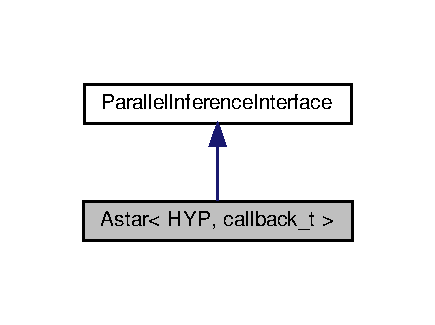
\includegraphics[width=220pt]{class_astar__inherit__graph}
\end{center}
\end{figure}


Collaboration diagram for Astar$<$ H\+YP, callback\+\_\+t $>$\+:
\nopagebreak
\begin{figure}[H]
\begin{center}
\leavevmode
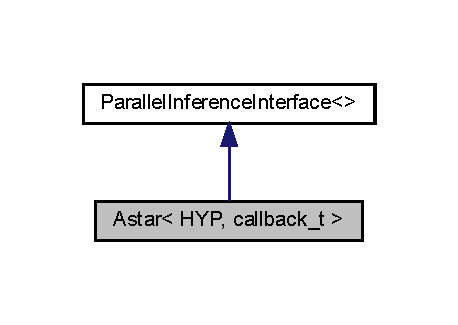
\includegraphics[width=220pt]{class_astar__coll__graph}
\end{center}
\end{figure}
\subsection*{Public Member Functions}
\begin{DoxyCompactItemize}
\item 
\hyperlink{class_astar_a5735f0f775bbaf1e2280b3220602596b}{Astar} (H\+YP \&h0, typename H\+Y\+P\+::data\+\_\+t $\ast$d, callback\+\_\+t \&cb, double temp)
\item 
void \hyperlink{class_astar_adc632480077c990ab12f88a85709b76f}{push} (H\+YP \&h)
\item 
void \hyperlink{class_astar_a689ddbddae5f21f26053d2d376c34095}{push} (H\+YP \&\&h)
\item 
void \hyperlink{class_astar_a962d234b6b109597c03516d61ff2cffc}{run\+\_\+thread} (\hyperlink{struct_control}{Control} ctl) override
\end{DoxyCompactItemize}
\subsection*{Public Attributes}
\begin{DoxyCompactItemize}
\item 
std\+::priority\+\_\+queue$<$ H\+YP, \hyperlink{class_reserved_vector}{Reserved\+Vector}$<$ H\+YP, \hyperlink{class_astar_af674f24278326383c5972fc30f0b21d9}{I\+N\+I\+T\+I\+A\+L\+\_\+\+S\+I\+ZE} $>$ $>$ \hyperlink{class_astar_af96593236e2f3ea3d15b37d513308391}{Q}
\end{DoxyCompactItemize}
\subsection*{Static Public Attributes}
\begin{DoxyCompactItemize}
\item 
static constexpr size\+\_\+t \hyperlink{class_astar_af674f24278326383c5972fc30f0b21d9}{I\+N\+I\+T\+I\+A\+L\+\_\+\+S\+I\+ZE} = 10000000
\item 
static constexpr size\+\_\+t \hyperlink{class_astar_a4086ae1c376d4d1b8d456f46f09cfa8a}{N\+\_\+\+R\+E\+PS} = 1
\item 
static constexpr double \hyperlink{class_astar_a111836518f01d8d4495d00e3b2a17531}{P\+A\+R\+E\+N\+T\+\_\+\+P\+E\+N\+A\+L\+TY} = 1.\+1
\item 
static double \hyperlink{class_astar_a9c708491f187aca582d7a3499a442bba}{temperature} = 100.\+0
\item 
static callback\+\_\+t $\ast$ \hyperlink{class_astar_a73b7b4ac7d9bdea8b8ce19c94c901705}{callback} = nullptr
\item 
static H\+Y\+P\+::data\+\_\+t $\ast$ \hyperlink{class_astar_a6b4ed5bb7ce08dcdceea3697d4f8eb2b}{data} = nullptr
\end{DoxyCompactItemize}


\subsection{Detailed Description}
\subsubsection*{template$<$typename H\+YP, typename callback\+\_\+t$>$\newline
class Astar$<$ H\+Y\+P, callback\+\_\+t $>$}

\begin{DoxyAuthor}{Author}
piantado 
\end{DoxyAuthor}
\begin{DoxyDate}{Date}
07/06/20 
\end{DoxyDate}


\subsection{Constructor \& Destructor Documentation}
\mbox{\Hypertarget{class_astar_a5735f0f775bbaf1e2280b3220602596b}\label{class_astar_a5735f0f775bbaf1e2280b3220602596b}} 
\index{Astar@{Astar}!Astar@{Astar}}
\index{Astar@{Astar}!Astar@{Astar}}
\subsubsection{\texorpdfstring{Astar()}{Astar()}}
{\footnotesize\ttfamily template$<$typename H\+YP , typename callback\+\_\+t $>$ \\
\hyperlink{class_astar}{Astar}$<$ H\+YP, callback\+\_\+t $>$\+::\hyperlink{class_astar}{Astar} (\begin{DoxyParamCaption}\item[{H\+YP \&}]{h0,  }\item[{typename H\+Y\+P\+::data\+\_\+t $\ast$}]{d,  }\item[{callback\+\_\+t \&}]{cb,  }\item[{double}]{temp }\end{DoxyParamCaption})\hspace{0.3cm}{\ttfamily [inline]}}



\subsection{Member Function Documentation}
\mbox{\Hypertarget{class_astar_adc632480077c990ab12f88a85709b76f}\label{class_astar_adc632480077c990ab12f88a85709b76f}} 
\index{Astar@{Astar}!push@{push}}
\index{push@{push}!Astar@{Astar}}
\subsubsection{\texorpdfstring{push()}{push()}\hspace{0.1cm}{\footnotesize\ttfamily [1/2]}}
{\footnotesize\ttfamily template$<$typename H\+YP , typename callback\+\_\+t $>$ \\
void \hyperlink{class_astar}{Astar}$<$ H\+YP, callback\+\_\+t $>$\+::push (\begin{DoxyParamCaption}\item[{H\+YP \&}]{h }\end{DoxyParamCaption})\hspace{0.3cm}{\ttfamily [inline]}}

\mbox{\Hypertarget{class_astar_a689ddbddae5f21f26053d2d376c34095}\label{class_astar_a689ddbddae5f21f26053d2d376c34095}} 
\index{Astar@{Astar}!push@{push}}
\index{push@{push}!Astar@{Astar}}
\subsubsection{\texorpdfstring{push()}{push()}\hspace{0.1cm}{\footnotesize\ttfamily [2/2]}}
{\footnotesize\ttfamily template$<$typename H\+YP , typename callback\+\_\+t $>$ \\
void \hyperlink{class_astar}{Astar}$<$ H\+YP, callback\+\_\+t $>$\+::push (\begin{DoxyParamCaption}\item[{H\+YP \&\&}]{h }\end{DoxyParamCaption})\hspace{0.3cm}{\ttfamily [inline]}}

\mbox{\Hypertarget{class_astar_a962d234b6b109597c03516d61ff2cffc}\label{class_astar_a962d234b6b109597c03516d61ff2cffc}} 
\index{Astar@{Astar}!run\+\_\+thread@{run\+\_\+thread}}
\index{run\+\_\+thread@{run\+\_\+thread}!Astar@{Astar}}
\subsubsection{\texorpdfstring{run\+\_\+thread()}{run\_thread()}}
{\footnotesize\ttfamily template$<$typename H\+YP , typename callback\+\_\+t $>$ \\
void \hyperlink{class_astar}{Astar}$<$ H\+YP, callback\+\_\+t $>$\+::run\+\_\+thread (\begin{DoxyParamCaption}\item[{\hyperlink{struct_control}{Control}}]{ctl }\end{DoxyParamCaption})\hspace{0.3cm}{\ttfamily [inline]}, {\ttfamily [override]}}



\subsection{Member Data Documentation}
\mbox{\Hypertarget{class_astar_a73b7b4ac7d9bdea8b8ce19c94c901705}\label{class_astar_a73b7b4ac7d9bdea8b8ce19c94c901705}} 
\index{Astar@{Astar}!callback@{callback}}
\index{callback@{callback}!Astar@{Astar}}
\subsubsection{\texorpdfstring{callback}{callback}}
{\footnotesize\ttfamily template$<$typename H\+YP , typename callback\+\_\+t $>$ \\
callback\+\_\+t $\ast$ \hyperlink{class_astar}{Astar}$<$ H\+YP, callback\+\_\+t $>$\+::callback = nullptr\hspace{0.3cm}{\ttfamily [static]}}

\mbox{\Hypertarget{class_astar_a6b4ed5bb7ce08dcdceea3697d4f8eb2b}\label{class_astar_a6b4ed5bb7ce08dcdceea3697d4f8eb2b}} 
\index{Astar@{Astar}!data@{data}}
\index{data@{data}!Astar@{Astar}}
\subsubsection{\texorpdfstring{data}{data}}
{\footnotesize\ttfamily template$<$typename H\+YP , typename callback\+\_\+t $>$ \\
H\+Y\+P\+::data\+\_\+t $\ast$ \hyperlink{class_astar}{Astar}$<$ H\+YP, callback\+\_\+t $>$\+::data = nullptr\hspace{0.3cm}{\ttfamily [static]}}

\mbox{\Hypertarget{class_astar_af674f24278326383c5972fc30f0b21d9}\label{class_astar_af674f24278326383c5972fc30f0b21d9}} 
\index{Astar@{Astar}!I\+N\+I\+T\+I\+A\+L\+\_\+\+S\+I\+ZE@{I\+N\+I\+T\+I\+A\+L\+\_\+\+S\+I\+ZE}}
\index{I\+N\+I\+T\+I\+A\+L\+\_\+\+S\+I\+ZE@{I\+N\+I\+T\+I\+A\+L\+\_\+\+S\+I\+ZE}!Astar@{Astar}}
\subsubsection{\texorpdfstring{I\+N\+I\+T\+I\+A\+L\+\_\+\+S\+I\+ZE}{INITIAL\_SIZE}}
{\footnotesize\ttfamily template$<$typename H\+YP , typename callback\+\_\+t $>$ \\
constexpr size\+\_\+t \hyperlink{class_astar}{Astar}$<$ H\+YP, callback\+\_\+t $>$\+::I\+N\+I\+T\+I\+A\+L\+\_\+\+S\+I\+ZE = 10000000\hspace{0.3cm}{\ttfamily [static]}}

\mbox{\Hypertarget{class_astar_a4086ae1c376d4d1b8d456f46f09cfa8a}\label{class_astar_a4086ae1c376d4d1b8d456f46f09cfa8a}} 
\index{Astar@{Astar}!N\+\_\+\+R\+E\+PS@{N\+\_\+\+R\+E\+PS}}
\index{N\+\_\+\+R\+E\+PS@{N\+\_\+\+R\+E\+PS}!Astar@{Astar}}
\subsubsection{\texorpdfstring{N\+\_\+\+R\+E\+PS}{N\_REPS}}
{\footnotesize\ttfamily template$<$typename H\+YP , typename callback\+\_\+t $>$ \\
constexpr size\+\_\+t \hyperlink{class_astar}{Astar}$<$ H\+YP, callback\+\_\+t $>$\+::N\+\_\+\+R\+E\+PS = 1\hspace{0.3cm}{\ttfamily [static]}}

\mbox{\Hypertarget{class_astar_a111836518f01d8d4495d00e3b2a17531}\label{class_astar_a111836518f01d8d4495d00e3b2a17531}} 
\index{Astar@{Astar}!P\+A\+R\+E\+N\+T\+\_\+\+P\+E\+N\+A\+L\+TY@{P\+A\+R\+E\+N\+T\+\_\+\+P\+E\+N\+A\+L\+TY}}
\index{P\+A\+R\+E\+N\+T\+\_\+\+P\+E\+N\+A\+L\+TY@{P\+A\+R\+E\+N\+T\+\_\+\+P\+E\+N\+A\+L\+TY}!Astar@{Astar}}
\subsubsection{\texorpdfstring{P\+A\+R\+E\+N\+T\+\_\+\+P\+E\+N\+A\+L\+TY}{PARENT\_PENALTY}}
{\footnotesize\ttfamily template$<$typename H\+YP , typename callback\+\_\+t $>$ \\
constexpr double \hyperlink{class_astar}{Astar}$<$ H\+YP, callback\+\_\+t $>$\+::P\+A\+R\+E\+N\+T\+\_\+\+P\+E\+N\+A\+L\+TY = 1.\+1\hspace{0.3cm}{\ttfamily [static]}}

\mbox{\Hypertarget{class_astar_af96593236e2f3ea3d15b37d513308391}\label{class_astar_af96593236e2f3ea3d15b37d513308391}} 
\index{Astar@{Astar}!Q@{Q}}
\index{Q@{Q}!Astar@{Astar}}
\subsubsection{\texorpdfstring{Q}{Q}}
{\footnotesize\ttfamily template$<$typename H\+YP , typename callback\+\_\+t $>$ \\
std\+::priority\+\_\+queue$<$H\+YP, \hyperlink{class_reserved_vector}{Reserved\+Vector}$<$H\+YP,\hyperlink{class_astar_af674f24278326383c5972fc30f0b21d9}{I\+N\+I\+T\+I\+A\+L\+\_\+\+S\+I\+ZE}$>$ $>$ \hyperlink{class_astar}{Astar}$<$ H\+YP, callback\+\_\+t $>$\+::Q}

\mbox{\Hypertarget{class_astar_a9c708491f187aca582d7a3499a442bba}\label{class_astar_a9c708491f187aca582d7a3499a442bba}} 
\index{Astar@{Astar}!temperature@{temperature}}
\index{temperature@{temperature}!Astar@{Astar}}
\subsubsection{\texorpdfstring{temperature}{temperature}}
{\footnotesize\ttfamily template$<$typename H\+YP , typename callback\+\_\+t $>$ \\
double \hyperlink{class_astar}{Astar}$<$ H\+YP, callback\+\_\+t $>$\+::temperature = 100.\+0\hspace{0.3cm}{\ttfamily [static]}}



The documentation for this class was generated from the following file\+:\begin{DoxyCompactItemize}
\item 
src/\+Inference/\hyperlink{_astar_8h}{Astar.\+h}\end{DoxyCompactItemize}

\hypertarget{class_base_node}{}\doxysection{Base\+Node$<$ this\+\_\+t $>$ Class Template Reference}
\label{class_base_node}\index{BaseNode$<$ this\_t $>$@{BaseNode$<$ this\_t $>$}}


{\ttfamily \#include $<$Base\+Node.\+h$>$}



Inheritance diagram for Base\+Node$<$ this\+\_\+t $>$\+:
\nopagebreak
\begin{figure}[H]
\begin{center}
\leavevmode
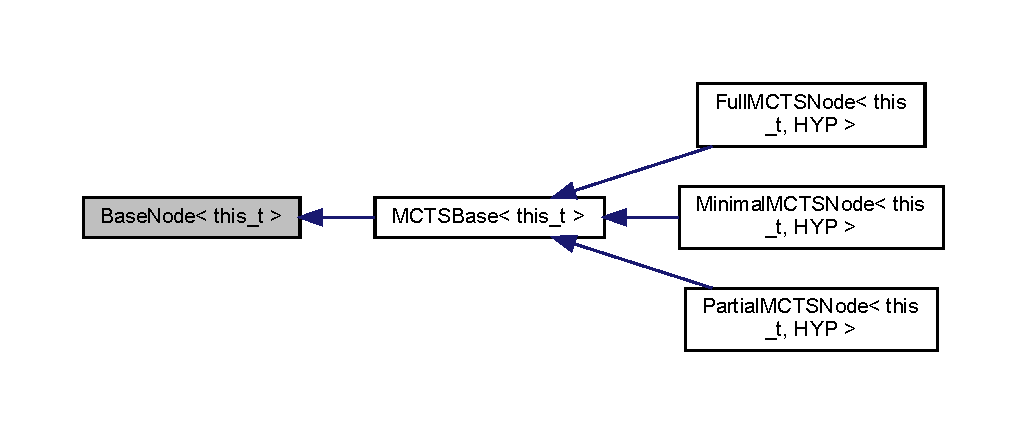
\includegraphics[width=350pt]{class_base_node__inherit__graph}
\end{center}
\end{figure}


Collaboration diagram for Base\+Node$<$ this\+\_\+t $>$\+:
\nopagebreak
\begin{figure}[H]
\begin{center}
\leavevmode
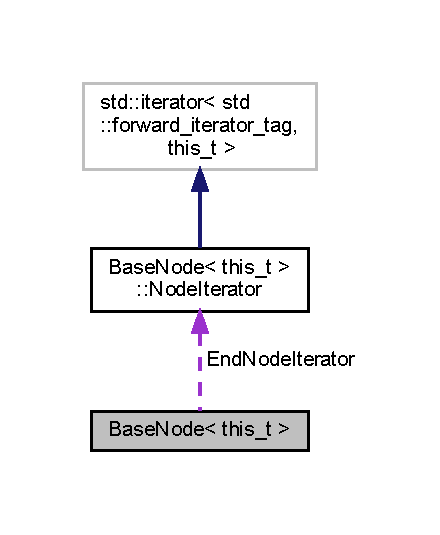
\includegraphics[width=211pt]{class_base_node__coll__graph}
\end{center}
\end{figure}
\doxysubsection*{Classes}
\begin{DoxyCompactItemize}
\item 
class \mbox{\hyperlink{class_base_node_1_1_node_iterator}{Node\+Iterator}}
\end{DoxyCompactItemize}
\doxysubsection*{Public Member Functions}
\begin{DoxyCompactItemize}
\item 
\mbox{\hyperlink{class_base_node_ae6af9c22d332e9c3158d9467f77b59f7}{Base\+Node}} (size\+\_\+t n=0, this\+\_\+t $\ast$p=nullptr, size\+\_\+t i=0)
\begin{DoxyCompactList}\small\item\em Constructor of basenode -- sizes children to n. \end{DoxyCompactList}\item 
\mbox{\hyperlink{class_base_node_a4bad5d46ee19af54c1385771bb6c8380}{Base\+Node}} (const this\+\_\+t \&n)
\item 
\mbox{\hyperlink{class_base_node_ab42ef3f5a20566523577925ab0c2a911}{Base\+Node}} (this\+\_\+t \&\&n)
\item 
void \mbox{\hyperlink{class_base_node_a1a82f7670d09cdd2a7f12e00513b1d8f}{operator=}} (const this\+\_\+t \&t)
\item 
void \mbox{\hyperlink{class_base_node_adc129f52a6d44237b7e8c62c65f8332c}{operator=}} (const this\+\_\+t \&\&t)
\item 
void \mbox{\hyperlink{class_base_node_a8c3616d00244a5e0fc7c15a8d584da98}{make\+\_\+root}} ()
\begin{DoxyCompactList}\small\item\em Make a node root -- just nulls the parent. \end{DoxyCompactList}\item 
virtual \mbox{\hyperlink{class_base_node_a2a33248b0eb051d7672691a73a38ff12}{$\sim$\+Base\+Node}} ()
\item 
virtual std\+::string \mbox{\hyperlink{class_base_node_a079dae7bec84f4de8eef6d6cb9368a22}{string}} (bool usedot=true) const
\item 
virtual std\+::string \mbox{\hyperlink{class_base_node_a263b93d5aaf1ce5eb7f103bf3b988db3}{my\+\_\+string}} () const
\item 
virtual bool \mbox{\hyperlink{class_base_node_a33bb5c59122f6b2778d39a0eaa0151d7}{operator==}} (const this\+\_\+t \&n) const
\item 
\mbox{\hyperlink{class_base_node_1_1_node_iterator}{Node\+Iterator}} \mbox{\hyperlink{class_base_node_ac735dd6fe296af4b8d2951cc6d9052c8}{begin}} () const
\item 
\mbox{\hyperlink{class_base_node_1_1_node_iterator}{Node\+Iterator}} \mbox{\hyperlink{class_base_node_a990f4bbfab3e8c78421e51f32cb5db48}{end}} () const
\item 
virtual bool \mbox{\hyperlink{class_base_node_a2f0418334eb790283f8074c9a27fed6e}{operator!=}} (const this\+\_\+t \&n) const
\item 
void \mbox{\hyperlink{class_base_node_abb32a7d0574ed17ddeb61e7262d090ad}{reserve\+\_\+children}} (const size\+\_\+t n)
\item 
decltype(\mbox{\hyperlink{class_base_node_af2f245862083d173c950fca048c03546}{children}}) \& \mbox{\hyperlink{class_base_node_a7177763ffa8b3e658124c586dde30be9}{get\+\_\+children}} ()
\item 
decltype(\mbox{\hyperlink{class_base_node_af2f245862083d173c950fca048c03546}{children}}) const  \& \mbox{\hyperlink{class_base_node_aec98c1640e03a27d1663f876bc49ef69}{get\+\_\+children}} () const
\item 
this\+\_\+t \& \mbox{\hyperlink{class_base_node_ac2ed3b362a2563e86063a157daa1c288}{child}} (const size\+\_\+t i)
\item 
const this\+\_\+t \& \mbox{\hyperlink{class_base_node_a2e244ddbbc0edea5f648e2a900e9dd99}{child}} (const size\+\_\+t i) const
\item 
{\footnotesize template$<$typename... Args$>$ }\\void \mbox{\hyperlink{class_base_node_aa7e88efda898c45f84ab0d79d4bb85c2}{fill}} (size\+\_\+t n, Args... args)
\item 
size\+\_\+t \mbox{\hyperlink{class_base_node_abae4d16401a958dc41d2852dedcf0721}{nchildren}} () const
\item 
this\+\_\+t $\ast$ \mbox{\hyperlink{class_base_node_ad319f28caf14e730bc62560f1bd682b6}{left\+\_\+descend}} () const
\item 
size\+\_\+t \mbox{\hyperlink{class_base_node_a4bab446840126b79f4d70cdc9bc6974c}{depth}} () const
\item 
void \mbox{\hyperlink{class_base_node_ad0ef64be7c40f1e9f9170d8d51f8d3bf}{fix\+\_\+child\+\_\+info}} ()
\item 
void \mbox{\hyperlink{class_base_node_a83b33d8a8902819b4175b66fb6e4b08e}{check\+\_\+child\+\_\+info}} () const
\item 
this\+\_\+t \& \mbox{\hyperlink{class_base_node_a6aec587267d880a8f87312d90e74af56}{operator\mbox{[}$\,$\mbox{]}}} (const size\+\_\+t i)
\item 
const this\+\_\+t \& \mbox{\hyperlink{class_base_node_ad09bee05b19581e8827bdd03a31791a7}{operator\mbox{[}$\,$\mbox{]}}} (const size\+\_\+t i) const
\item 
void \mbox{\hyperlink{class_base_node_af6fd9f209baeb7b4799b1a1da5fc6897}{set\+\_\+child}} (const size\+\_\+t i, this\+\_\+t \&n)
\item 
void \mbox{\hyperlink{class_base_node_a5eb63d66f3d2aa4194aae33fa72bddc9}{set\+\_\+child}} (const size\+\_\+t i, this\+\_\+t \&\&n)
\item 
void \mbox{\hyperlink{class_base_node_ab5a808e3ec22f8061022f9ec286d4a03}{push\+\_\+back}} (this\+\_\+t \&n)
\item 
void \mbox{\hyperlink{class_base_node_a6971173d807967deda4501eb70676533}{push\+\_\+back}} (this\+\_\+t \&\&n)
\item 
virtual bool \mbox{\hyperlink{class_base_node_afce604388d562d347fcb31aeb2a8ef03}{is\+\_\+root}} () const
\begin{DoxyCompactList}\small\item\em Am I a root node? I am if my parent is nullptr. \end{DoxyCompactList}\item 
this\+\_\+t $\ast$ \mbox{\hyperlink{class_base_node_ab953456c09fa01bbf8a29c07f4d2b5ad}{root}} ()
\begin{DoxyCompactList}\small\item\em Find the root of this node by walking up the tree. \end{DoxyCompactList}\item 
this\+\_\+t $\ast$ \mbox{\hyperlink{class_base_node_add31235ad96e659230cbca6c9e357523}{get\+\_\+via}} (std\+::function$<$ bool(this\+\_\+t \&)$>$ \&f)
\begin{DoxyCompactList}\small\item\em Return a pointer to the first node satisfying predicate f, in standard traversal; nullptr otherwise. \end{DoxyCompactList}\item 
virtual size\+\_\+t \mbox{\hyperlink{class_base_node_a4007d1c72991b8599a6ff5a21c054ba5}{count}} () const
\begin{DoxyCompactList}\small\item\em How many nodes total are below me? \end{DoxyCompactList}\item 
virtual size\+\_\+t \mbox{\hyperlink{class_base_node_aaaf113bd98ee404e71582ac1cf014ac0}{count}} (const this\+\_\+t \&n) const
\begin{DoxyCompactList}\small\item\em How many nodes below me are equal to n? \end{DoxyCompactList}\item 
virtual bool \mbox{\hyperlink{class_base_node_af37331cbec1b32c874138d2ae9b89745}{is\+\_\+terminal}} () const
\begin{DoxyCompactList}\small\item\em Am I a terminal? I am if I have no children. \end{DoxyCompactList}\item 
virtual size\+\_\+t \mbox{\hyperlink{class_base_node_adb6326eefe4ddc311651b4a4a5cb119e}{count\+\_\+terminals}} () const
\item 
virtual this\+\_\+t $\ast$ \mbox{\hyperlink{class_base_node_a1e4560f882d4cdb713aea5178a4e2d86}{get\+\_\+nth}} (int n, std\+::function$<$ int(const this\+\_\+t \&)$>$ \&f)
\item 
virtual this\+\_\+t $\ast$ \mbox{\hyperlink{class_base_node_a9381814fdc86029905dc283da5d3d931}{get\+\_\+nth}} (int n)
\item 
{\footnotesize template$<$typename T $>$ }\\T \mbox{\hyperlink{class_base_node_a32872bacb6a7c7e8f592a0abdb6dbb6d}{sum}} (std\+::function$<$ T(const this\+\_\+t \&)$>$ \&f) const
\item 
{\footnotesize template$<$typename T $>$ }\\T \mbox{\hyperlink{class_base_node_a1d71d0fee70974903720768c86a98d03}{sum}} (T($\ast$f)(const this\+\_\+t \&)) const
\item 
bool \mbox{\hyperlink{class_base_node_ab534dfbdebd79785db3971336ef34418}{all}} (std\+::function$<$ bool(const this\+\_\+t \&)$>$ \&f) const
\item 
void \mbox{\hyperlink{class_base_node_a56bc19ee155443b7600cf8a2e7db38cb}{map}} (const std\+::function$<$ void(this\+\_\+t \&)$>$ \&f)
\item 
void \mbox{\hyperlink{class_base_node_acbfcc951fe5858d0c85a5b3dc8843f05}{print}} (size\+\_\+t t=0) const
\end{DoxyCompactItemize}
\doxysubsection*{Public Attributes}
\begin{DoxyCompactItemize}
\item 
this\+\_\+t $\ast$ \mbox{\hyperlink{class_base_node_aa1ad671f67931a82120d5852520417b7}{parent}}
\item 
size\+\_\+t \mbox{\hyperlink{class_base_node_a6e2caf1ce4e3f0436c277b7331dbd554}{pi}}
\end{DoxyCompactItemize}
\doxysubsection*{Static Public Attributes}
\begin{DoxyCompactItemize}
\item 
static \mbox{\hyperlink{class_base_node_1_1_node_iterator}{Node\+Iterator}} \mbox{\hyperlink{class_base_node_ac8a2fe45180446f4db2d4742c34b5b80}{End\+Node\+Iterator}} = \mbox{\hyperlink{class_base_node_1_1_node_iterator}{Node\+Iterator}}(nullptr)
\end{DoxyCompactItemize}
\doxysubsection*{Protected Attributes}
\begin{DoxyCompactItemize}
\item 
std\+::vector$<$ this\+\_\+t $>$ \mbox{\hyperlink{class_base_node_af2f245862083d173c950fca048c03546}{children}}
\end{DoxyCompactItemize}


\doxysubsection{Detailed Description}
\subsubsection*{template$<$typename this\+\_\+t$>$\newline
class Base\+Node$<$ this\+\_\+t $>$}

\begin{DoxyAuthor}{Author}
piantado 
\end{DoxyAuthor}
\begin{DoxyDate}{Date}
03/07/20 
\end{DoxyDate}


\doxysubsection{Constructor \& Destructor Documentation}
\mbox{\Hypertarget{class_base_node_ae6af9c22d332e9c3158d9467f77b59f7}\label{class_base_node_ae6af9c22d332e9c3158d9467f77b59f7}} 
\index{BaseNode$<$ this\_t $>$@{BaseNode$<$ this\_t $>$}!BaseNode@{BaseNode}}
\index{BaseNode@{BaseNode}!BaseNode$<$ this\_t $>$@{BaseNode$<$ this\_t $>$}}
\doxysubsubsection{\texorpdfstring{BaseNode()}{BaseNode()}\hspace{0.1cm}{\footnotesize\ttfamily [1/3]}}
{\footnotesize\ttfamily template$<$typename this\+\_\+t $>$ \\
\mbox{\hyperlink{class_base_node}{Base\+Node}}$<$ this\+\_\+t $>$\+::\mbox{\hyperlink{class_base_node}{Base\+Node}} (\begin{DoxyParamCaption}\item[{size\+\_\+t}]{n = {\ttfamily 0},  }\item[{this\+\_\+t $\ast$}]{p = {\ttfamily nullptr},  }\item[{size\+\_\+t}]{i = {\ttfamily 0} }\end{DoxyParamCaption})\hspace{0.3cm}{\ttfamily [inline]}}



Constructor of basenode -- sizes children to n. 


\begin{DoxyParams}{Parameters}
{\em n} & \\
\hline
{\em p} & \\
\hline
{\em i} & \\
\hline
\end{DoxyParams}
\mbox{\Hypertarget{class_base_node_a4bad5d46ee19af54c1385771bb6c8380}\label{class_base_node_a4bad5d46ee19af54c1385771bb6c8380}} 
\index{BaseNode$<$ this\_t $>$@{BaseNode$<$ this\_t $>$}!BaseNode@{BaseNode}}
\index{BaseNode@{BaseNode}!BaseNode$<$ this\_t $>$@{BaseNode$<$ this\_t $>$}}
\doxysubsubsection{\texorpdfstring{BaseNode()}{BaseNode()}\hspace{0.1cm}{\footnotesize\ttfamily [2/3]}}
{\footnotesize\ttfamily template$<$typename this\+\_\+t $>$ \\
\mbox{\hyperlink{class_base_node}{Base\+Node}}$<$ this\+\_\+t $>$\+::\mbox{\hyperlink{class_base_node}{Base\+Node}} (\begin{DoxyParamCaption}\item[{const this\+\_\+t \&}]{n }\end{DoxyParamCaption})\hspace{0.3cm}{\ttfamily [inline]}}

\mbox{\Hypertarget{class_base_node_ab42ef3f5a20566523577925ab0c2a911}\label{class_base_node_ab42ef3f5a20566523577925ab0c2a911}} 
\index{BaseNode$<$ this\_t $>$@{BaseNode$<$ this\_t $>$}!BaseNode@{BaseNode}}
\index{BaseNode@{BaseNode}!BaseNode$<$ this\_t $>$@{BaseNode$<$ this\_t $>$}}
\doxysubsubsection{\texorpdfstring{BaseNode()}{BaseNode()}\hspace{0.1cm}{\footnotesize\ttfamily [3/3]}}
{\footnotesize\ttfamily template$<$typename this\+\_\+t $>$ \\
\mbox{\hyperlink{class_base_node}{Base\+Node}}$<$ this\+\_\+t $>$\+::\mbox{\hyperlink{class_base_node}{Base\+Node}} (\begin{DoxyParamCaption}\item[{this\+\_\+t \&\&}]{n }\end{DoxyParamCaption})\hspace{0.3cm}{\ttfamily [inline]}}

\mbox{\Hypertarget{class_base_node_a2a33248b0eb051d7672691a73a38ff12}\label{class_base_node_a2a33248b0eb051d7672691a73a38ff12}} 
\index{BaseNode$<$ this\_t $>$@{BaseNode$<$ this\_t $>$}!````~BaseNode@{$\sim$BaseNode}}
\index{````~BaseNode@{$\sim$BaseNode}!BaseNode$<$ this\_t $>$@{BaseNode$<$ this\_t $>$}}
\doxysubsubsection{\texorpdfstring{$\sim$BaseNode()}{~BaseNode()}}
{\footnotesize\ttfamily template$<$typename this\+\_\+t $>$ \\
virtual \mbox{\hyperlink{class_base_node}{Base\+Node}}$<$ this\+\_\+t $>$\+::$\sim$\mbox{\hyperlink{class_base_node}{Base\+Node}} (\begin{DoxyParamCaption}{ }\end{DoxyParamCaption})\hspace{0.3cm}{\ttfamily [inline]}, {\ttfamily [virtual]}}



\doxysubsection{Member Function Documentation}
\mbox{\Hypertarget{class_base_node_ab534dfbdebd79785db3971336ef34418}\label{class_base_node_ab534dfbdebd79785db3971336ef34418}} 
\index{BaseNode$<$ this\_t $>$@{BaseNode$<$ this\_t $>$}!all@{all}}
\index{all@{all}!BaseNode$<$ this\_t $>$@{BaseNode$<$ this\_t $>$}}
\doxysubsubsection{\texorpdfstring{all()}{all()}}
{\footnotesize\ttfamily template$<$typename this\+\_\+t $>$ \\
bool \mbox{\hyperlink{class_base_node}{Base\+Node}}$<$ this\+\_\+t $>$\+::all (\begin{DoxyParamCaption}\item[{std\+::function$<$ bool(const this\+\_\+t \&)$>$ \&}]{f }\end{DoxyParamCaption}) const\hspace{0.3cm}{\ttfamily [inline]}}

Check if f is true of me and every node below 
\begin{DoxyParams}{Parameters}
{\em f} & \\
\hline
\end{DoxyParams}
\begin{DoxyReturn}{Returns}

\end{DoxyReturn}
\mbox{\Hypertarget{class_base_node_ac735dd6fe296af4b8d2951cc6d9052c8}\label{class_base_node_ac735dd6fe296af4b8d2951cc6d9052c8}} 
\index{BaseNode$<$ this\_t $>$@{BaseNode$<$ this\_t $>$}!begin@{begin}}
\index{begin@{begin}!BaseNode$<$ this\_t $>$@{BaseNode$<$ this\_t $>$}}
\doxysubsubsection{\texorpdfstring{begin()}{begin()}}
{\footnotesize\ttfamily template$<$typename this\+\_\+t $>$ \\
\mbox{\hyperlink{class_base_node_1_1_node_iterator}{Node\+Iterator}} \mbox{\hyperlink{class_base_node}{Base\+Node}}$<$ this\+\_\+t $>$\+::begin (\begin{DoxyParamCaption}{ }\end{DoxyParamCaption}) const\hspace{0.3cm}{\ttfamily [inline]}}

\mbox{\Hypertarget{class_base_node_a83b33d8a8902819b4175b66fb6e4b08e}\label{class_base_node_a83b33d8a8902819b4175b66fb6e4b08e}} 
\index{BaseNode$<$ this\_t $>$@{BaseNode$<$ this\_t $>$}!check\_child\_info@{check\_child\_info}}
\index{check\_child\_info@{check\_child\_info}!BaseNode$<$ this\_t $>$@{BaseNode$<$ this\_t $>$}}
\doxysubsubsection{\texorpdfstring{check\_child\_info()}{check\_child\_info()}}
{\footnotesize\ttfamily template$<$typename this\+\_\+t $>$ \\
void \mbox{\hyperlink{class_base_node}{Base\+Node}}$<$ this\+\_\+t $>$\+::check\+\_\+child\+\_\+info (\begin{DoxyParamCaption}{ }\end{DoxyParamCaption}) const\hspace{0.3cm}{\ttfamily [inline]}}

assert that all of the child info is correct\mbox{\Hypertarget{class_base_node_ac2ed3b362a2563e86063a157daa1c288}\label{class_base_node_ac2ed3b362a2563e86063a157daa1c288}} 
\index{BaseNode$<$ this\_t $>$@{BaseNode$<$ this\_t $>$}!child@{child}}
\index{child@{child}!BaseNode$<$ this\_t $>$@{BaseNode$<$ this\_t $>$}}
\doxysubsubsection{\texorpdfstring{child()}{child()}\hspace{0.1cm}{\footnotesize\ttfamily [1/2]}}
{\footnotesize\ttfamily template$<$typename this\+\_\+t $>$ \\
this\+\_\+t\& \mbox{\hyperlink{class_base_node}{Base\+Node}}$<$ this\+\_\+t $>$\+::child (\begin{DoxyParamCaption}\item[{const size\+\_\+t}]{i }\end{DoxyParamCaption})\hspace{0.3cm}{\ttfamily [inline]}}

Get a reference to my i\textquotesingle{}th child 
\begin{DoxyParams}{Parameters}
{\em i} & \\
\hline
\end{DoxyParams}
\begin{DoxyReturn}{Returns}

\end{DoxyReturn}
\mbox{\Hypertarget{class_base_node_a2e244ddbbc0edea5f648e2a900e9dd99}\label{class_base_node_a2e244ddbbc0edea5f648e2a900e9dd99}} 
\index{BaseNode$<$ this\_t $>$@{BaseNode$<$ this\_t $>$}!child@{child}}
\index{child@{child}!BaseNode$<$ this\_t $>$@{BaseNode$<$ this\_t $>$}}
\doxysubsubsection{\texorpdfstring{child()}{child()}\hspace{0.1cm}{\footnotesize\ttfamily [2/2]}}
{\footnotesize\ttfamily template$<$typename this\+\_\+t $>$ \\
const this\+\_\+t\& \mbox{\hyperlink{class_base_node}{Base\+Node}}$<$ this\+\_\+t $>$\+::child (\begin{DoxyParamCaption}\item[{const size\+\_\+t}]{i }\end{DoxyParamCaption}) const\hspace{0.3cm}{\ttfamily [inline]}}

Constant reference to the i\textquotesingle{}th child 
\begin{DoxyParams}{Parameters}
{\em i} & \\
\hline
\end{DoxyParams}
\begin{DoxyReturn}{Returns}

\end{DoxyReturn}
\mbox{\Hypertarget{class_base_node_a4007d1c72991b8599a6ff5a21c054ba5}\label{class_base_node_a4007d1c72991b8599a6ff5a21c054ba5}} 
\index{BaseNode$<$ this\_t $>$@{BaseNode$<$ this\_t $>$}!count@{count}}
\index{count@{count}!BaseNode$<$ this\_t $>$@{BaseNode$<$ this\_t $>$}}
\doxysubsubsection{\texorpdfstring{count()}{count()}\hspace{0.1cm}{\footnotesize\ttfamily [1/2]}}
{\footnotesize\ttfamily template$<$typename this\+\_\+t $>$ \\
virtual size\+\_\+t \mbox{\hyperlink{class_base_node}{Base\+Node}}$<$ this\+\_\+t $>$\+::count (\begin{DoxyParamCaption}{ }\end{DoxyParamCaption}) const\hspace{0.3cm}{\ttfamily [inline]}, {\ttfamily [virtual]}}



How many nodes total are below me? 


\begin{DoxyParams}{Parameters}
{\em n} & \\
\hline
\end{DoxyParams}
\begin{DoxyReturn}{Returns}

\end{DoxyReturn}
\mbox{\Hypertarget{class_base_node_aaaf113bd98ee404e71582ac1cf014ac0}\label{class_base_node_aaaf113bd98ee404e71582ac1cf014ac0}} 
\index{BaseNode$<$ this\_t $>$@{BaseNode$<$ this\_t $>$}!count@{count}}
\index{count@{count}!BaseNode$<$ this\_t $>$@{BaseNode$<$ this\_t $>$}}
\doxysubsubsection{\texorpdfstring{count()}{count()}\hspace{0.1cm}{\footnotesize\ttfamily [2/2]}}
{\footnotesize\ttfamily template$<$typename this\+\_\+t $>$ \\
virtual size\+\_\+t \mbox{\hyperlink{class_base_node}{Base\+Node}}$<$ this\+\_\+t $>$\+::count (\begin{DoxyParamCaption}\item[{const this\+\_\+t \&}]{n }\end{DoxyParamCaption}) const\hspace{0.3cm}{\ttfamily [inline]}, {\ttfamily [virtual]}}



How many nodes below me are equal to n? 


\begin{DoxyParams}{Parameters}
{\em n} & \\
\hline
\end{DoxyParams}
\begin{DoxyReturn}{Returns}

\end{DoxyReturn}
\mbox{\Hypertarget{class_base_node_adb6326eefe4ddc311651b4a4a5cb119e}\label{class_base_node_adb6326eefe4ddc311651b4a4a5cb119e}} 
\index{BaseNode$<$ this\_t $>$@{BaseNode$<$ this\_t $>$}!count\_terminals@{count\_terminals}}
\index{count\_terminals@{count\_terminals}!BaseNode$<$ this\_t $>$@{BaseNode$<$ this\_t $>$}}
\doxysubsubsection{\texorpdfstring{count\_terminals()}{count\_terminals()}}
{\footnotesize\ttfamily template$<$typename this\+\_\+t $>$ \\
virtual size\+\_\+t \mbox{\hyperlink{class_base_node}{Base\+Node}}$<$ this\+\_\+t $>$\+::count\+\_\+terminals (\begin{DoxyParamCaption}{ }\end{DoxyParamCaption}) const\hspace{0.3cm}{\ttfamily [inline]}, {\ttfamily [virtual]}}

How many terminals are below me? \begin{DoxyReturn}{Returns}

\end{DoxyReturn}
\mbox{\Hypertarget{class_base_node_a4bab446840126b79f4d70cdc9bc6974c}\label{class_base_node_a4bab446840126b79f4d70cdc9bc6974c}} 
\index{BaseNode$<$ this\_t $>$@{BaseNode$<$ this\_t $>$}!depth@{depth}}
\index{depth@{depth}!BaseNode$<$ this\_t $>$@{BaseNode$<$ this\_t $>$}}
\doxysubsubsection{\texorpdfstring{depth()}{depth()}}
{\footnotesize\ttfamily template$<$typename this\+\_\+t $>$ \\
size\+\_\+t \mbox{\hyperlink{class_base_node}{Base\+Node}}$<$ this\+\_\+t $>$\+::depth (\begin{DoxyParamCaption}{ }\end{DoxyParamCaption}) const\hspace{0.3cm}{\ttfamily [inline]}}

\mbox{\Hypertarget{class_base_node_a990f4bbfab3e8c78421e51f32cb5db48}\label{class_base_node_a990f4bbfab3e8c78421e51f32cb5db48}} 
\index{BaseNode$<$ this\_t $>$@{BaseNode$<$ this\_t $>$}!end@{end}}
\index{end@{end}!BaseNode$<$ this\_t $>$@{BaseNode$<$ this\_t $>$}}
\doxysubsubsection{\texorpdfstring{end()}{end()}}
{\footnotesize\ttfamily template$<$typename this\+\_\+t $>$ \\
\mbox{\hyperlink{class_base_node_1_1_node_iterator}{Node\+Iterator}} \mbox{\hyperlink{class_base_node}{Base\+Node}}$<$ this\+\_\+t $>$\+::end (\begin{DoxyParamCaption}{ }\end{DoxyParamCaption}) const\hspace{0.3cm}{\ttfamily [inline]}}

\mbox{\Hypertarget{class_base_node_aa7e88efda898c45f84ab0d79d4bb85c2}\label{class_base_node_aa7e88efda898c45f84ab0d79d4bb85c2}} 
\index{BaseNode$<$ this\_t $>$@{BaseNode$<$ this\_t $>$}!fill@{fill}}
\index{fill@{fill}!BaseNode$<$ this\_t $>$@{BaseNode$<$ this\_t $>$}}
\doxysubsubsection{\texorpdfstring{fill()}{fill()}}
{\footnotesize\ttfamily template$<$typename this\+\_\+t $>$ \\
template$<$typename... Args$>$ \\
void \mbox{\hyperlink{class_base_node}{Base\+Node}}$<$ this\+\_\+t $>$\+::fill (\begin{DoxyParamCaption}\item[{size\+\_\+t}]{n,  }\item[{Args...}]{args }\end{DoxyParamCaption})\hspace{0.3cm}{\ttfamily [inline]}}

Fill in all of my immediate children with Null nodes (via Null\+Rule)\mbox{\Hypertarget{class_base_node_ad0ef64be7c40f1e9f9170d8d51f8d3bf}\label{class_base_node_ad0ef64be7c40f1e9f9170d8d51f8d3bf}} 
\index{BaseNode$<$ this\_t $>$@{BaseNode$<$ this\_t $>$}!fix\_child\_info@{fix\_child\_info}}
\index{fix\_child\_info@{fix\_child\_info}!BaseNode$<$ this\_t $>$@{BaseNode$<$ this\_t $>$}}
\doxysubsubsection{\texorpdfstring{fix\_child\_info()}{fix\_child\_info()}}
{\footnotesize\ttfamily template$<$typename this\+\_\+t $>$ \\
void \mbox{\hyperlink{class_base_node}{Base\+Node}}$<$ this\+\_\+t $>$\+::fix\+\_\+child\+\_\+info (\begin{DoxyParamCaption}{ }\end{DoxyParamCaption})\hspace{0.3cm}{\ttfamily [inline]}}

Fix my immediate children\textquotesingle{}s pointers to ensure that children\textquotesingle{}s parent pointers and indices are correct.\mbox{\Hypertarget{class_base_node_a7177763ffa8b3e658124c586dde30be9}\label{class_base_node_a7177763ffa8b3e658124c586dde30be9}} 
\index{BaseNode$<$ this\_t $>$@{BaseNode$<$ this\_t $>$}!get\_children@{get\_children}}
\index{get\_children@{get\_children}!BaseNode$<$ this\_t $>$@{BaseNode$<$ this\_t $>$}}
\doxysubsubsection{\texorpdfstring{get\_children()}{get\_children()}\hspace{0.1cm}{\footnotesize\ttfamily [1/2]}}
{\footnotesize\ttfamily template$<$typename this\+\_\+t $>$ \\
decltype(\mbox{\hyperlink{class_base_node_af2f245862083d173c950fca048c03546}{children}}) \& \mbox{\hyperlink{class_base_node}{Base\+Node}}$<$ this\+\_\+t $>$\+::get\+\_\+children (\begin{DoxyParamCaption}{ }\end{DoxyParamCaption})\hspace{0.3cm}{\ttfamily [inline]}}

\mbox{\Hypertarget{class_base_node_aec98c1640e03a27d1663f876bc49ef69}\label{class_base_node_aec98c1640e03a27d1663f876bc49ef69}} 
\index{BaseNode$<$ this\_t $>$@{BaseNode$<$ this\_t $>$}!get\_children@{get\_children}}
\index{get\_children@{get\_children}!BaseNode$<$ this\_t $>$@{BaseNode$<$ this\_t $>$}}
\doxysubsubsection{\texorpdfstring{get\_children()}{get\_children()}\hspace{0.1cm}{\footnotesize\ttfamily [2/2]}}
{\footnotesize\ttfamily template$<$typename this\+\_\+t $>$ \\
decltype(\mbox{\hyperlink{class_base_node_af2f245862083d173c950fca048c03546}{children}}) const\& \mbox{\hyperlink{class_base_node}{Base\+Node}}$<$ this\+\_\+t $>$\+::get\+\_\+children (\begin{DoxyParamCaption}{ }\end{DoxyParamCaption}) const\hspace{0.3cm}{\ttfamily [inline]}}

\mbox{\Hypertarget{class_base_node_a9381814fdc86029905dc283da5d3d931}\label{class_base_node_a9381814fdc86029905dc283da5d3d931}} 
\index{BaseNode$<$ this\_t $>$@{BaseNode$<$ this\_t $>$}!get\_nth@{get\_nth}}
\index{get\_nth@{get\_nth}!BaseNode$<$ this\_t $>$@{BaseNode$<$ this\_t $>$}}
\doxysubsubsection{\texorpdfstring{get\_nth()}{get\_nth()}\hspace{0.1cm}{\footnotesize\ttfamily [1/2]}}
{\footnotesize\ttfamily template$<$typename this\+\_\+t $>$ \\
virtual this\+\_\+t$\ast$ \mbox{\hyperlink{class_base_node}{Base\+Node}}$<$ this\+\_\+t $>$\+::get\+\_\+nth (\begin{DoxyParamCaption}\item[{int}]{n }\end{DoxyParamCaption})\hspace{0.3cm}{\ttfamily [inline]}, {\ttfamily [virtual]}}

\mbox{\Hypertarget{class_base_node_a1e4560f882d4cdb713aea5178a4e2d86}\label{class_base_node_a1e4560f882d4cdb713aea5178a4e2d86}} 
\index{BaseNode$<$ this\_t $>$@{BaseNode$<$ this\_t $>$}!get\_nth@{get\_nth}}
\index{get\_nth@{get\_nth}!BaseNode$<$ this\_t $>$@{BaseNode$<$ this\_t $>$}}
\doxysubsubsection{\texorpdfstring{get\_nth()}{get\_nth()}\hspace{0.1cm}{\footnotesize\ttfamily [2/2]}}
{\footnotesize\ttfamily template$<$typename this\+\_\+t $>$ \\
virtual this\+\_\+t$\ast$ \mbox{\hyperlink{class_base_node}{Base\+Node}}$<$ this\+\_\+t $>$\+::get\+\_\+nth (\begin{DoxyParamCaption}\item[{int}]{n,  }\item[{std\+::function$<$ int(const this\+\_\+t \&)$>$ \&}]{f }\end{DoxyParamCaption})\hspace{0.3cm}{\ttfamily [inline]}, {\ttfamily [virtual]}}

Return a pointer to the n\textquotesingle{}th child satisfying f (f\textquotesingle{}s output is cast to bool) 
\begin{DoxyParams}{Parameters}
{\em n} & \\
\hline
{\em f} & \\
\hline
\end{DoxyParams}
\begin{DoxyReturn}{Returns}

\end{DoxyReturn}
\mbox{\Hypertarget{class_base_node_add31235ad96e659230cbca6c9e357523}\label{class_base_node_add31235ad96e659230cbca6c9e357523}} 
\index{BaseNode$<$ this\_t $>$@{BaseNode$<$ this\_t $>$}!get\_via@{get\_via}}
\index{get\_via@{get\_via}!BaseNode$<$ this\_t $>$@{BaseNode$<$ this\_t $>$}}
\doxysubsubsection{\texorpdfstring{get\_via()}{get\_via()}}
{\footnotesize\ttfamily template$<$typename this\+\_\+t $>$ \\
this\+\_\+t$\ast$ \mbox{\hyperlink{class_base_node}{Base\+Node}}$<$ this\+\_\+t $>$\+::get\+\_\+via (\begin{DoxyParamCaption}\item[{std\+::function$<$ bool(this\+\_\+t \&)$>$ \&}]{f }\end{DoxyParamCaption})\hspace{0.3cm}{\ttfamily [inline]}}



Return a pointer to the first node satisfying predicate f, in standard traversal; nullptr otherwise. 


\begin{DoxyParams}{Parameters}
{\em f} & \\
\hline
\end{DoxyParams}
\begin{DoxyReturn}{Returns}

\end{DoxyReturn}
\mbox{\Hypertarget{class_base_node_afce604388d562d347fcb31aeb2a8ef03}\label{class_base_node_afce604388d562d347fcb31aeb2a8ef03}} 
\index{BaseNode$<$ this\_t $>$@{BaseNode$<$ this\_t $>$}!is\_root@{is\_root}}
\index{is\_root@{is\_root}!BaseNode$<$ this\_t $>$@{BaseNode$<$ this\_t $>$}}
\doxysubsubsection{\texorpdfstring{is\_root()}{is\_root()}}
{\footnotesize\ttfamily template$<$typename this\+\_\+t $>$ \\
virtual bool \mbox{\hyperlink{class_base_node}{Base\+Node}}$<$ this\+\_\+t $>$\+::is\+\_\+root (\begin{DoxyParamCaption}{ }\end{DoxyParamCaption}) const\hspace{0.3cm}{\ttfamily [inline]}, {\ttfamily [virtual]}}



Am I a root node? I am if my parent is nullptr. 

\begin{DoxyReturn}{Returns}

\end{DoxyReturn}
\mbox{\Hypertarget{class_base_node_af37331cbec1b32c874138d2ae9b89745}\label{class_base_node_af37331cbec1b32c874138d2ae9b89745}} 
\index{BaseNode$<$ this\_t $>$@{BaseNode$<$ this\_t $>$}!is\_terminal@{is\_terminal}}
\index{is\_terminal@{is\_terminal}!BaseNode$<$ this\_t $>$@{BaseNode$<$ this\_t $>$}}
\doxysubsubsection{\texorpdfstring{is\_terminal()}{is\_terminal()}}
{\footnotesize\ttfamily template$<$typename this\+\_\+t $>$ \\
virtual bool \mbox{\hyperlink{class_base_node}{Base\+Node}}$<$ this\+\_\+t $>$\+::is\+\_\+terminal (\begin{DoxyParamCaption}{ }\end{DoxyParamCaption}) const\hspace{0.3cm}{\ttfamily [inline]}, {\ttfamily [virtual]}}



Am I a terminal? I am if I have no children. 

\begin{DoxyReturn}{Returns}

\end{DoxyReturn}
\mbox{\Hypertarget{class_base_node_ad319f28caf14e730bc62560f1bd682b6}\label{class_base_node_ad319f28caf14e730bc62560f1bd682b6}} 
\index{BaseNode$<$ this\_t $>$@{BaseNode$<$ this\_t $>$}!left\_descend@{left\_descend}}
\index{left\_descend@{left\_descend}!BaseNode$<$ this\_t $>$@{BaseNode$<$ this\_t $>$}}
\doxysubsubsection{\texorpdfstring{left\_descend()}{left\_descend()}}
{\footnotesize\ttfamily template$<$typename this\+\_\+t $>$ \\
this\+\_\+t$\ast$ \mbox{\hyperlink{class_base_node}{Base\+Node}}$<$ this\+\_\+t $>$\+::left\+\_\+descend (\begin{DoxyParamCaption}{ }\end{DoxyParamCaption}) const\hspace{0.3cm}{\ttfamily [inline]}}

Go down a tree and find the leftmost child \begin{DoxyReturn}{Returns}

\end{DoxyReturn}
\mbox{\Hypertarget{class_base_node_a8c3616d00244a5e0fc7c15a8d584da98}\label{class_base_node_a8c3616d00244a5e0fc7c15a8d584da98}} 
\index{BaseNode$<$ this\_t $>$@{BaseNode$<$ this\_t $>$}!make\_root@{make\_root}}
\index{make\_root@{make\_root}!BaseNode$<$ this\_t $>$@{BaseNode$<$ this\_t $>$}}
\doxysubsubsection{\texorpdfstring{make\_root()}{make\_root()}}
{\footnotesize\ttfamily template$<$typename this\+\_\+t $>$ \\
void \mbox{\hyperlink{class_base_node}{Base\+Node}}$<$ this\+\_\+t $>$\+::make\+\_\+root (\begin{DoxyParamCaption}{ }\end{DoxyParamCaption})\hspace{0.3cm}{\ttfamily [inline]}}



Make a node root -- just nulls the parent. 

\mbox{\Hypertarget{class_base_node_a56bc19ee155443b7600cf8a2e7db38cb}\label{class_base_node_a56bc19ee155443b7600cf8a2e7db38cb}} 
\index{BaseNode$<$ this\_t $>$@{BaseNode$<$ this\_t $>$}!map@{map}}
\index{map@{map}!BaseNode$<$ this\_t $>$@{BaseNode$<$ this\_t $>$}}
\doxysubsubsection{\texorpdfstring{map()}{map()}}
{\footnotesize\ttfamily template$<$typename this\+\_\+t $>$ \\
void \mbox{\hyperlink{class_base_node}{Base\+Node}}$<$ this\+\_\+t $>$\+::map (\begin{DoxyParamCaption}\item[{const std\+::function$<$ void(this\+\_\+t \&)$>$ \&}]{f }\end{DoxyParamCaption})\hspace{0.3cm}{\ttfamily [inline]}}

Apply f to me and everything below. ~\newline
 
\begin{DoxyParams}{Parameters}
{\em f} & \\
\hline
\end{DoxyParams}
\mbox{\Hypertarget{class_base_node_a263b93d5aaf1ce5eb7f103bf3b988db3}\label{class_base_node_a263b93d5aaf1ce5eb7f103bf3b988db3}} 
\index{BaseNode$<$ this\_t $>$@{BaseNode$<$ this\_t $>$}!my\_string@{my\_string}}
\index{my\_string@{my\_string}!BaseNode$<$ this\_t $>$@{BaseNode$<$ this\_t $>$}}
\doxysubsubsection{\texorpdfstring{my\_string()}{my\_string()}}
{\footnotesize\ttfamily template$<$typename this\+\_\+t $>$ \\
virtual std\+::string \mbox{\hyperlink{class_base_node}{Base\+Node}}$<$ this\+\_\+t $>$\+::my\+\_\+string (\begin{DoxyParamCaption}{ }\end{DoxyParamCaption}) const\hspace{0.3cm}{\ttfamily [inline]}, {\ttfamily [virtual]}}

just print myself, not all my kids (single row per node display)\mbox{\Hypertarget{class_base_node_abae4d16401a958dc41d2852dedcf0721}\label{class_base_node_abae4d16401a958dc41d2852dedcf0721}} 
\index{BaseNode$<$ this\_t $>$@{BaseNode$<$ this\_t $>$}!nchildren@{nchildren}}
\index{nchildren@{nchildren}!BaseNode$<$ this\_t $>$@{BaseNode$<$ this\_t $>$}}
\doxysubsubsection{\texorpdfstring{nchildren()}{nchildren()}}
{\footnotesize\ttfamily template$<$typename this\+\_\+t $>$ \\
size\+\_\+t \mbox{\hyperlink{class_base_node}{Base\+Node}}$<$ this\+\_\+t $>$\+::nchildren (\begin{DoxyParamCaption}{ }\end{DoxyParamCaption}) const\hspace{0.3cm}{\ttfamily [inline]}}

How many children do I have? \begin{DoxyReturn}{Returns}

\end{DoxyReturn}
\mbox{\Hypertarget{class_base_node_a2f0418334eb790283f8074c9a27fed6e}\label{class_base_node_a2f0418334eb790283f8074c9a27fed6e}} 
\index{BaseNode$<$ this\_t $>$@{BaseNode$<$ this\_t $>$}!operator"!=@{operator"!=}}
\index{operator"!=@{operator"!=}!BaseNode$<$ this\_t $>$@{BaseNode$<$ this\_t $>$}}
\doxysubsubsection{\texorpdfstring{operator"!=()}{operator!=()}}
{\footnotesize\ttfamily template$<$typename this\+\_\+t $>$ \\
virtual bool \mbox{\hyperlink{class_base_node}{Base\+Node}}$<$ this\+\_\+t $>$\+::operator!= (\begin{DoxyParamCaption}\item[{const this\+\_\+t \&}]{n }\end{DoxyParamCaption}) const\hspace{0.3cm}{\ttfamily [inline]}, {\ttfamily [virtual]}}

\mbox{\Hypertarget{class_base_node_adc129f52a6d44237b7e8c62c65f8332c}\label{class_base_node_adc129f52a6d44237b7e8c62c65f8332c}} 
\index{BaseNode$<$ this\_t $>$@{BaseNode$<$ this\_t $>$}!operator=@{operator=}}
\index{operator=@{operator=}!BaseNode$<$ this\_t $>$@{BaseNode$<$ this\_t $>$}}
\doxysubsubsection{\texorpdfstring{operator=()}{operator=()}\hspace{0.1cm}{\footnotesize\ttfamily [1/2]}}
{\footnotesize\ttfamily template$<$typename this\+\_\+t $>$ \\
void \mbox{\hyperlink{class_base_node}{Base\+Node}}$<$ this\+\_\+t $>$\+::operator= (\begin{DoxyParamCaption}\item[{const this\+\_\+t \&\&}]{t }\end{DoxyParamCaption})\hspace{0.3cm}{\ttfamily [inline]}}

\mbox{\Hypertarget{class_base_node_a1a82f7670d09cdd2a7f12e00513b1d8f}\label{class_base_node_a1a82f7670d09cdd2a7f12e00513b1d8f}} 
\index{BaseNode$<$ this\_t $>$@{BaseNode$<$ this\_t $>$}!operator=@{operator=}}
\index{operator=@{operator=}!BaseNode$<$ this\_t $>$@{BaseNode$<$ this\_t $>$}}
\doxysubsubsection{\texorpdfstring{operator=()}{operator=()}\hspace{0.1cm}{\footnotesize\ttfamily [2/2]}}
{\footnotesize\ttfamily template$<$typename this\+\_\+t $>$ \\
void \mbox{\hyperlink{class_base_node}{Base\+Node}}$<$ this\+\_\+t $>$\+::operator= (\begin{DoxyParamCaption}\item[{const this\+\_\+t \&}]{t }\end{DoxyParamCaption})\hspace{0.3cm}{\ttfamily [inline]}}

\mbox{\Hypertarget{class_base_node_a33bb5c59122f6b2778d39a0eaa0151d7}\label{class_base_node_a33bb5c59122f6b2778d39a0eaa0151d7}} 
\index{BaseNode$<$ this\_t $>$@{BaseNode$<$ this\_t $>$}!operator==@{operator==}}
\index{operator==@{operator==}!BaseNode$<$ this\_t $>$@{BaseNode$<$ this\_t $>$}}
\doxysubsubsection{\texorpdfstring{operator==()}{operator==()}}
{\footnotesize\ttfamily template$<$typename this\+\_\+t $>$ \\
virtual bool \mbox{\hyperlink{class_base_node}{Base\+Node}}$<$ this\+\_\+t $>$\+::operator== (\begin{DoxyParamCaption}\item[{const this\+\_\+t \&}]{n }\end{DoxyParamCaption}) const\hspace{0.3cm}{\ttfamily [inline]}, {\ttfamily [virtual]}}



Reimplemented in \mbox{\hyperlink{class_node_a8f42de356c047dd52472d24ace4d42c5}{Node}}.

\mbox{\Hypertarget{class_base_node_a6aec587267d880a8f87312d90e74af56}\label{class_base_node_a6aec587267d880a8f87312d90e74af56}} 
\index{BaseNode$<$ this\_t $>$@{BaseNode$<$ this\_t $>$}!operator\mbox{[}\mbox{]}@{operator[]}}
\index{operator\mbox{[}\mbox{]}@{operator[]}!BaseNode$<$ this\_t $>$@{BaseNode$<$ this\_t $>$}}
\doxysubsubsection{\texorpdfstring{operator[]()}{operator[]()}\hspace{0.1cm}{\footnotesize\ttfamily [1/2]}}
{\footnotesize\ttfamily template$<$typename this\+\_\+t $>$ \\
this\+\_\+t\& \mbox{\hyperlink{class_base_node}{Base\+Node}}$<$ this\+\_\+t $>$\+::operator\mbox{[}$\,$\mbox{]} (\begin{DoxyParamCaption}\item[{const size\+\_\+t}]{i }\end{DoxyParamCaption})\hspace{0.3cm}{\ttfamily [inline]}}

Index my i\textquotesingle{}th child 
\begin{DoxyParams}{Parameters}
{\em i} & \\
\hline
\end{DoxyParams}
\begin{DoxyReturn}{Returns}

\end{DoxyReturn}
\mbox{\Hypertarget{class_base_node_ad09bee05b19581e8827bdd03a31791a7}\label{class_base_node_ad09bee05b19581e8827bdd03a31791a7}} 
\index{BaseNode$<$ this\_t $>$@{BaseNode$<$ this\_t $>$}!operator\mbox{[}\mbox{]}@{operator[]}}
\index{operator\mbox{[}\mbox{]}@{operator[]}!BaseNode$<$ this\_t $>$@{BaseNode$<$ this\_t $>$}}
\doxysubsubsection{\texorpdfstring{operator[]()}{operator[]()}\hspace{0.1cm}{\footnotesize\ttfamily [2/2]}}
{\footnotesize\ttfamily template$<$typename this\+\_\+t $>$ \\
const this\+\_\+t\& \mbox{\hyperlink{class_base_node}{Base\+Node}}$<$ this\+\_\+t $>$\+::operator\mbox{[}$\,$\mbox{]} (\begin{DoxyParamCaption}\item[{const size\+\_\+t}]{i }\end{DoxyParamCaption}) const\hspace{0.3cm}{\ttfamily [inline]}}

\mbox{\Hypertarget{class_base_node_acbfcc951fe5858d0c85a5b3dc8843f05}\label{class_base_node_acbfcc951fe5858d0c85a5b3dc8843f05}} 
\index{BaseNode$<$ this\_t $>$@{BaseNode$<$ this\_t $>$}!print@{print}}
\index{print@{print}!BaseNode$<$ this\_t $>$@{BaseNode$<$ this\_t $>$}}
\doxysubsubsection{\texorpdfstring{print()}{print()}}
{\footnotesize\ttfamily template$<$typename this\+\_\+t $>$ \\
void \mbox{\hyperlink{class_base_node}{Base\+Node}}$<$ this\+\_\+t $>$\+::\mbox{\hyperlink{structprint}{print}} (\begin{DoxyParamCaption}\item[{size\+\_\+t}]{t = {\ttfamily 0} }\end{DoxyParamCaption}) const\hspace{0.3cm}{\ttfamily [inline]}}

\mbox{\Hypertarget{class_base_node_a6971173d807967deda4501eb70676533}\label{class_base_node_a6971173d807967deda4501eb70676533}} 
\index{BaseNode$<$ this\_t $>$@{BaseNode$<$ this\_t $>$}!push\_back@{push\_back}}
\index{push\_back@{push\_back}!BaseNode$<$ this\_t $>$@{BaseNode$<$ this\_t $>$}}
\doxysubsubsection{\texorpdfstring{push\_back()}{push\_back()}\hspace{0.1cm}{\footnotesize\ttfamily [1/2]}}
{\footnotesize\ttfamily template$<$typename this\+\_\+t $>$ \\
void \mbox{\hyperlink{class_base_node}{Base\+Node}}$<$ this\+\_\+t $>$\+::push\+\_\+back (\begin{DoxyParamCaption}\item[{this\+\_\+t \&\&}]{n }\end{DoxyParamCaption})\hspace{0.3cm}{\ttfamily [inline]}}

\mbox{\Hypertarget{class_base_node_ab5a808e3ec22f8061022f9ec286d4a03}\label{class_base_node_ab5a808e3ec22f8061022f9ec286d4a03}} 
\index{BaseNode$<$ this\_t $>$@{BaseNode$<$ this\_t $>$}!push\_back@{push\_back}}
\index{push\_back@{push\_back}!BaseNode$<$ this\_t $>$@{BaseNode$<$ this\_t $>$}}
\doxysubsubsection{\texorpdfstring{push\_back()}{push\_back()}\hspace{0.1cm}{\footnotesize\ttfamily [2/2]}}
{\footnotesize\ttfamily template$<$typename this\+\_\+t $>$ \\
void \mbox{\hyperlink{class_base_node}{Base\+Node}}$<$ this\+\_\+t $>$\+::push\+\_\+back (\begin{DoxyParamCaption}\item[{this\+\_\+t \&}]{n }\end{DoxyParamCaption})\hspace{0.3cm}{\ttfamily [inline]}}

\mbox{\Hypertarget{class_base_node_abb32a7d0574ed17ddeb61e7262d090ad}\label{class_base_node_abb32a7d0574ed17ddeb61e7262d090ad}} 
\index{BaseNode$<$ this\_t $>$@{BaseNode$<$ this\_t $>$}!reserve\_children@{reserve\_children}}
\index{reserve\_children@{reserve\_children}!BaseNode$<$ this\_t $>$@{BaseNode$<$ this\_t $>$}}
\doxysubsubsection{\texorpdfstring{reserve\_children()}{reserve\_children()}}
{\footnotesize\ttfamily template$<$typename this\+\_\+t $>$ \\
void \mbox{\hyperlink{class_base_node}{Base\+Node}}$<$ this\+\_\+t $>$\+::reserve\+\_\+children (\begin{DoxyParamCaption}\item[{const size\+\_\+t}]{n }\end{DoxyParamCaption})\hspace{0.3cm}{\ttfamily [inline]}}

\mbox{\Hypertarget{class_base_node_ab953456c09fa01bbf8a29c07f4d2b5ad}\label{class_base_node_ab953456c09fa01bbf8a29c07f4d2b5ad}} 
\index{BaseNode$<$ this\_t $>$@{BaseNode$<$ this\_t $>$}!root@{root}}
\index{root@{root}!BaseNode$<$ this\_t $>$@{BaseNode$<$ this\_t $>$}}
\doxysubsubsection{\texorpdfstring{root()}{root()}}
{\footnotesize\ttfamily template$<$typename this\+\_\+t $>$ \\
this\+\_\+t$\ast$ \mbox{\hyperlink{class_base_node}{Base\+Node}}$<$ this\+\_\+t $>$\+::root (\begin{DoxyParamCaption}{ }\end{DoxyParamCaption})\hspace{0.3cm}{\ttfamily [inline]}}



Find the root of this node by walking up the tree. 

\begin{DoxyReturn}{Returns}

\end{DoxyReturn}
\mbox{\Hypertarget{class_base_node_a5eb63d66f3d2aa4194aae33fa72bddc9}\label{class_base_node_a5eb63d66f3d2aa4194aae33fa72bddc9}} 
\index{BaseNode$<$ this\_t $>$@{BaseNode$<$ this\_t $>$}!set\_child@{set\_child}}
\index{set\_child@{set\_child}!BaseNode$<$ this\_t $>$@{BaseNode$<$ this\_t $>$}}
\doxysubsubsection{\texorpdfstring{set\_child()}{set\_child()}\hspace{0.1cm}{\footnotesize\ttfamily [1/2]}}
{\footnotesize\ttfamily template$<$typename this\+\_\+t $>$ \\
void \mbox{\hyperlink{class_base_node}{Base\+Node}}$<$ this\+\_\+t $>$\+::set\+\_\+child (\begin{DoxyParamCaption}\item[{const size\+\_\+t}]{i,  }\item[{this\+\_\+t \&\&}]{n }\end{DoxyParamCaption})\hspace{0.3cm}{\ttfamily [inline]}}

Child setter for move 
\begin{DoxyParams}{Parameters}
{\em i} & \\
\hline
\end{DoxyParams}
\mbox{\Hypertarget{class_base_node_af6fd9f209baeb7b4799b1a1da5fc6897}\label{class_base_node_af6fd9f209baeb7b4799b1a1da5fc6897}} 
\index{BaseNode$<$ this\_t $>$@{BaseNode$<$ this\_t $>$}!set\_child@{set\_child}}
\index{set\_child@{set\_child}!BaseNode$<$ this\_t $>$@{BaseNode$<$ this\_t $>$}}
\doxysubsubsection{\texorpdfstring{set\_child()}{set\_child()}\hspace{0.1cm}{\footnotesize\ttfamily [2/2]}}
{\footnotesize\ttfamily template$<$typename this\+\_\+t $>$ \\
void \mbox{\hyperlink{class_base_node}{Base\+Node}}$<$ this\+\_\+t $>$\+::set\+\_\+child (\begin{DoxyParamCaption}\item[{const size\+\_\+t}]{i,  }\item[{this\+\_\+t \&}]{n }\end{DoxyParamCaption})\hspace{0.3cm}{\ttfamily [inline]}}

Set my child to n. N\+O\+TE\+: This one needs to be used, rather than accessing children directly, because we have to set parent pointers and indices. 
\begin{DoxyParams}{Parameters}
{\em i} & \\
\hline
{\em n} & \\
\hline
\end{DoxyParams}
\mbox{\Hypertarget{class_base_node_a079dae7bec84f4de8eef6d6cb9368a22}\label{class_base_node_a079dae7bec84f4de8eef6d6cb9368a22}} 
\index{BaseNode$<$ this\_t $>$@{BaseNode$<$ this\_t $>$}!string@{string}}
\index{string@{string}!BaseNode$<$ this\_t $>$@{BaseNode$<$ this\_t $>$}}
\doxysubsubsection{\texorpdfstring{string()}{string()}}
{\footnotesize\ttfamily template$<$typename this\+\_\+t $>$ \\
virtual std\+::string \mbox{\hyperlink{class_base_node}{Base\+Node}}$<$ this\+\_\+t $>$\+::string (\begin{DoxyParamCaption}\item[{bool}]{usedot = {\ttfamily true} }\end{DoxyParamCaption}) const\hspace{0.3cm}{\ttfamily [inline]}, {\ttfamily [virtual]}}



Reimplemented in \mbox{\hyperlink{class_node_a5d2a0e17dd2a00a79e6d1f763c9114d0}{Node}}.

\mbox{\Hypertarget{class_base_node_a32872bacb6a7c7e8f592a0abdb6dbb6d}\label{class_base_node_a32872bacb6a7c7e8f592a0abdb6dbb6d}} 
\index{BaseNode$<$ this\_t $>$@{BaseNode$<$ this\_t $>$}!sum@{sum}}
\index{sum@{sum}!BaseNode$<$ this\_t $>$@{BaseNode$<$ this\_t $>$}}
\doxysubsubsection{\texorpdfstring{sum()}{sum()}\hspace{0.1cm}{\footnotesize\ttfamily [1/2]}}
{\footnotesize\ttfamily template$<$typename this\+\_\+t $>$ \\
template$<$typename T $>$ \\
T \mbox{\hyperlink{class_base_node}{Base\+Node}}$<$ this\+\_\+t $>$\+::sum (\begin{DoxyParamCaption}\item[{std\+::function$<$ T(const this\+\_\+t \&)$>$ \&}]{f }\end{DoxyParamCaption}) const\hspace{0.3cm}{\ttfamily [inline]}}

Apply f to me and everything below me, adding up the result. 
\begin{DoxyParams}{Parameters}
{\em f} & \\
\hline
\end{DoxyParams}
\begin{DoxyReturn}{Returns}

\end{DoxyReturn}
\mbox{\Hypertarget{class_base_node_a1d71d0fee70974903720768c86a98d03}\label{class_base_node_a1d71d0fee70974903720768c86a98d03}} 
\index{BaseNode$<$ this\_t $>$@{BaseNode$<$ this\_t $>$}!sum@{sum}}
\index{sum@{sum}!BaseNode$<$ this\_t $>$@{BaseNode$<$ this\_t $>$}}
\doxysubsubsection{\texorpdfstring{sum()}{sum()}\hspace{0.1cm}{\footnotesize\ttfamily [2/2]}}
{\footnotesize\ttfamily template$<$typename this\+\_\+t $>$ \\
template$<$typename T $>$ \\
T \mbox{\hyperlink{class_base_node}{Base\+Node}}$<$ this\+\_\+t $>$\+::sum (\begin{DoxyParamCaption}\item[{T($\ast$)(const this\+\_\+t \&)}]{f }\end{DoxyParamCaption}) const\hspace{0.3cm}{\ttfamily [inline]}}



\doxysubsection{Member Data Documentation}
\mbox{\Hypertarget{class_base_node_af2f245862083d173c950fca048c03546}\label{class_base_node_af2f245862083d173c950fca048c03546}} 
\index{BaseNode$<$ this\_t $>$@{BaseNode$<$ this\_t $>$}!children@{children}}
\index{children@{children}!BaseNode$<$ this\_t $>$@{BaseNode$<$ this\_t $>$}}
\doxysubsubsection{\texorpdfstring{children}{children}}
{\footnotesize\ttfamily template$<$typename this\+\_\+t $>$ \\
std\+::vector$<$this\+\_\+t$>$ \mbox{\hyperlink{class_base_node}{Base\+Node}}$<$ this\+\_\+t $>$\+::children\hspace{0.3cm}{\ttfamily [protected]}}

\mbox{\Hypertarget{class_base_node_ac8a2fe45180446f4db2d4742c34b5b80}\label{class_base_node_ac8a2fe45180446f4db2d4742c34b5b80}} 
\index{BaseNode$<$ this\_t $>$@{BaseNode$<$ this\_t $>$}!EndNodeIterator@{EndNodeIterator}}
\index{EndNodeIterator@{EndNodeIterator}!BaseNode$<$ this\_t $>$@{BaseNode$<$ this\_t $>$}}
\doxysubsubsection{\texorpdfstring{EndNodeIterator}{EndNodeIterator}}
{\footnotesize\ttfamily template$<$typename this\+\_\+t $>$ \\
\mbox{\hyperlink{class_base_node}{Base\+Node}}$<$ this\+\_\+t $>$\+::\mbox{\hyperlink{class_base_node_1_1_node_iterator}{Node\+Iterator}} \mbox{\hyperlink{class_base_node}{Base\+Node}}$<$ this\+\_\+t $>$\+::End\+Node\+Iterator = \mbox{\hyperlink{class_base_node_1_1_node_iterator}{Node\+Iterator}}(nullptr)\hspace{0.3cm}{\ttfamily [static]}}

\mbox{\Hypertarget{class_base_node_aa1ad671f67931a82120d5852520417b7}\label{class_base_node_aa1ad671f67931a82120d5852520417b7}} 
\index{BaseNode$<$ this\_t $>$@{BaseNode$<$ this\_t $>$}!parent@{parent}}
\index{parent@{parent}!BaseNode$<$ this\_t $>$@{BaseNode$<$ this\_t $>$}}
\doxysubsubsection{\texorpdfstring{parent}{parent}}
{\footnotesize\ttfamily template$<$typename this\+\_\+t $>$ \\
this\+\_\+t$\ast$ \mbox{\hyperlink{class_base_node}{Base\+Node}}$<$ this\+\_\+t $>$\+::parent}

\mbox{\Hypertarget{class_base_node_a6e2caf1ce4e3f0436c277b7331dbd554}\label{class_base_node_a6e2caf1ce4e3f0436c277b7331dbd554}} 
\index{BaseNode$<$ this\_t $>$@{BaseNode$<$ this\_t $>$}!pi@{pi}}
\index{pi@{pi}!BaseNode$<$ this\_t $>$@{BaseNode$<$ this\_t $>$}}
\doxysubsubsection{\texorpdfstring{pi}{pi}}
{\footnotesize\ttfamily template$<$typename this\+\_\+t $>$ \\
size\+\_\+t \mbox{\hyperlink{class_base_node}{Base\+Node}}$<$ this\+\_\+t $>$\+::pi}



The documentation for this class was generated from the following file\+:\begin{DoxyCompactItemize}
\item 
src/\mbox{\hyperlink{_base_node_8h}{Base\+Node.\+h}}\end{DoxyCompactItemize}

\hypertarget{class_bayesable}{}\section{Bayesable$<$ \+\_\+datum\+\_\+t, \+\_\+data\+\_\+t $>$ Class Template Reference}
\label{class_bayesable}\index{Bayesable$<$ \+\_\+datum\+\_\+t, \+\_\+data\+\_\+t $>$@{Bayesable$<$ \+\_\+datum\+\_\+t, \+\_\+data\+\_\+t $>$}}


{\ttfamily \#include $<$Bayesable.\+h$>$}

\subsection*{Public Types}
\begin{DoxyCompactItemize}
\item 
typedef \+\_\+datum\+\_\+t \hyperlink{class_bayesable_a9f1a6c0cd7855550fa10b1a8f13a5867}{datum\+\_\+t}
\item 
typedef \+\_\+data\+\_\+t \hyperlink{class_bayesable_aa2788c4d7718c0a824e1d28c4c98f921}{data\+\_\+t}
\end{DoxyCompactItemize}
\subsection*{Public Member Functions}
\begin{DoxyCompactItemize}
\item 
\hyperlink{class_bayesable_aec41e7016c9c1eb6978e1360c23f20cd}{Bayesable} ()
\item 
virtual void \hyperlink{class_bayesable_ac8ab4bb38c8782d2dcd57f3a43a3c605}{clear\+\_\+bayes} ()
\item 
virtual double \hyperlink{class_bayesable_a1b057a17212ced123545133e2297c01b}{compute\+\_\+prior} ()=0
\begin{DoxyCompactList}\small\item\em Compute the prior -- defaultly not defined. \end{DoxyCompactList}\item 
virtual double \hyperlink{class_bayesable_a87d195bfe5cdf6d293dae5fc01ae2e6c}{compute\+\_\+single\+\_\+likelihood} (const \hyperlink{class_bayesable_a9f1a6c0cd7855550fa10b1a8f13a5867}{datum\+\_\+t} \&datum)
\begin{DoxyCompactList}\small\item\em Compute the likelihood of a single data point. \end{DoxyCompactList}\item 
virtual double \hyperlink{class_bayesable_a202493156cec15937bee304d807fdbdb}{compute\+\_\+likelihood} (const \hyperlink{class_bayesable_aa2788c4d7718c0a824e1d28c4c98f921}{data\+\_\+t} \&data, const double breakout=-\/\hyperlink{_numerics_8h_a1bb1e42ae1b40cad6e99da0aab8a5576}{infinity})
\begin{DoxyCompactList}\small\item\em Compute the likelihood of a collection of data, by calling compute\+\_\+single\+\_\+likelihood on each. This stops if our likelihood falls below breakout. \end{DoxyCompactList}\item 
virtual double \hyperlink{class_bayesable_a0b0552923602bcab6c768581ab8c7df8}{compute\+\_\+posterior} (const \hyperlink{class_bayesable_aa2788c4d7718c0a824e1d28c4c98f921}{data\+\_\+t} \&data, const double breakout=-\/\hyperlink{_numerics_8h_a1bb1e42ae1b40cad6e99da0aab8a5576}{infinity})
\item 
virtual double \hyperlink{class_bayesable_acf805473a9eea0df96d6267dca0e9c87}{at\+\_\+temperature} (double t)
\item 
virtual size\+\_\+t \hyperlink{class_bayesable_a26f6d55e7526ebd897cbb27c757b611b}{hash} () const =0
\begin{DoxyCompactList}\small\item\em Default hash function. \end{DoxyCompactList}\item 
virtual bool \hyperlink{class_bayesable_ac356e7e5b11c266b8442064186dbe89d}{operator$<$} (const \hyperlink{class_bayesable}{Bayesable}$<$ \hyperlink{class_bayesable_a9f1a6c0cd7855550fa10b1a8f13a5867}{datum\+\_\+t}, \hyperlink{class_bayesable_aa2788c4d7718c0a824e1d28c4c98f921}{data\+\_\+t} $>$ \&l) const
\item 
virtual std\+::string \hyperlink{class_bayesable_afcea9b439bcf321d5354710d8861cb54}{string} () const =0
\item 
virtual void \hyperlink{class_bayesable_a87d5d9481d6a72b017e44b175071fa5e}{print} (std\+::string prefix=\char`\"{}\char`\"{})
\end{DoxyCompactItemize}
\subsection*{Public Attributes}
\begin{DoxyCompactItemize}
\item 
double \hyperlink{class_bayesable_a473790922c2dd73e227350d029d73003}{prior}
\item 
double \hyperlink{class_bayesable_a4d1a9ed826013bf079cea1867b6d4183}{likelihood}
\item 
double \hyperlink{class_bayesable_a268442b9aae5b763c17ca29c39231915}{posterior}
\item 
uintmax\+\_\+t \hyperlink{class_bayesable_a898e03a20e1851c868b77ef4e844f0bf}{born}
\end{DoxyCompactItemize}


\subsection{Detailed Description}
\subsubsection*{template$<$typename \+\_\+datum\+\_\+t, typename \+\_\+data\+\_\+t = std\+::vector$<$\+\_\+datum\+\_\+t$>$$>$\newline
class Bayesable$<$ \+\_\+datum\+\_\+t, \+\_\+data\+\_\+t $>$}

\begin{DoxyAuthor}{Author}
steven piantadosi 
\end{DoxyAuthor}
\begin{DoxyDate}{Date}
29/01/20 
\end{DoxyDate}


\subsection{Member Typedef Documentation}
\mbox{\Hypertarget{class_bayesable_aa2788c4d7718c0a824e1d28c4c98f921}\label{class_bayesable_aa2788c4d7718c0a824e1d28c4c98f921}} 
\index{Bayesable@{Bayesable}!data\+\_\+t@{data\+\_\+t}}
\index{data\+\_\+t@{data\+\_\+t}!Bayesable@{Bayesable}}
\subsubsection{\texorpdfstring{data\+\_\+t}{data\_t}}
{\footnotesize\ttfamily template$<$typename \+\_\+datum\+\_\+t, typename \+\_\+data\+\_\+t = std\+::vector$<$\+\_\+datum\+\_\+t$>$$>$ \\
typedef \+\_\+data\+\_\+t \hyperlink{class_bayesable}{Bayesable}$<$ \+\_\+datum\+\_\+t, \+\_\+data\+\_\+t $>$\+::\hyperlink{class_bayesable_aa2788c4d7718c0a824e1d28c4c98f921}{data\+\_\+t}}

\mbox{\Hypertarget{class_bayesable_a9f1a6c0cd7855550fa10b1a8f13a5867}\label{class_bayesable_a9f1a6c0cd7855550fa10b1a8f13a5867}} 
\index{Bayesable@{Bayesable}!datum\+\_\+t@{datum\+\_\+t}}
\index{datum\+\_\+t@{datum\+\_\+t}!Bayesable@{Bayesable}}
\subsubsection{\texorpdfstring{datum\+\_\+t}{datum\_t}}
{\footnotesize\ttfamily template$<$typename \+\_\+datum\+\_\+t, typename \+\_\+data\+\_\+t = std\+::vector$<$\+\_\+datum\+\_\+t$>$$>$ \\
typedef \+\_\+datum\+\_\+t \hyperlink{class_bayesable}{Bayesable}$<$ \+\_\+datum\+\_\+t, \+\_\+data\+\_\+t $>$\+::\hyperlink{class_bayesable_a9f1a6c0cd7855550fa10b1a8f13a5867}{datum\+\_\+t}}



\subsection{Constructor \& Destructor Documentation}
\mbox{\Hypertarget{class_bayesable_aec41e7016c9c1eb6978e1360c23f20cd}\label{class_bayesable_aec41e7016c9c1eb6978e1360c23f20cd}} 
\index{Bayesable@{Bayesable}!Bayesable@{Bayesable}}
\index{Bayesable@{Bayesable}!Bayesable@{Bayesable}}
\subsubsection{\texorpdfstring{Bayesable()}{Bayesable()}}
{\footnotesize\ttfamily template$<$typename \+\_\+datum\+\_\+t, typename \+\_\+data\+\_\+t = std\+::vector$<$\+\_\+datum\+\_\+t$>$$>$ \\
\hyperlink{class_bayesable}{Bayesable}$<$ \+\_\+datum\+\_\+t, \+\_\+data\+\_\+t $>$\+::\hyperlink{class_bayesable}{Bayesable} (\begin{DoxyParamCaption}{ }\end{DoxyParamCaption})\hspace{0.3cm}{\ttfamily [inline]}}



\subsection{Member Function Documentation}
\mbox{\Hypertarget{class_bayesable_acf805473a9eea0df96d6267dca0e9c87}\label{class_bayesable_acf805473a9eea0df96d6267dca0e9c87}} 
\index{Bayesable@{Bayesable}!at\+\_\+temperature@{at\+\_\+temperature}}
\index{at\+\_\+temperature@{at\+\_\+temperature}!Bayesable@{Bayesable}}
\subsubsection{\texorpdfstring{at\+\_\+temperature()}{at\_temperature()}}
{\footnotesize\ttfamily template$<$typename \+\_\+datum\+\_\+t, typename \+\_\+data\+\_\+t = std\+::vector$<$\+\_\+datum\+\_\+t$>$$>$ \\
virtual double \hyperlink{class_bayesable}{Bayesable}$<$ \+\_\+datum\+\_\+t, \+\_\+data\+\_\+t $>$\+::at\+\_\+temperature (\begin{DoxyParamCaption}\item[{double}]{t }\end{DoxyParamCaption})\hspace{0.3cm}{\ttfamily [inline]}, {\ttfamily [virtual]}}

Return my posterior score at a given (likelihood) temperature 
\begin{DoxyParams}{Parameters}
{\em t} & \\
\hline
\end{DoxyParams}
\begin{DoxyReturn}{Returns}

\end{DoxyReturn}
\mbox{\Hypertarget{class_bayesable_ac8ab4bb38c8782d2dcd57f3a43a3c605}\label{class_bayesable_ac8ab4bb38c8782d2dcd57f3a43a3c605}} 
\index{Bayesable@{Bayesable}!clear\+\_\+bayes@{clear\+\_\+bayes}}
\index{clear\+\_\+bayes@{clear\+\_\+bayes}!Bayesable@{Bayesable}}
\subsubsection{\texorpdfstring{clear\+\_\+bayes()}{clear\_bayes()}}
{\footnotesize\ttfamily template$<$typename \+\_\+datum\+\_\+t, typename \+\_\+data\+\_\+t = std\+::vector$<$\+\_\+datum\+\_\+t$>$$>$ \\
virtual void \hyperlink{class_bayesable}{Bayesable}$<$ \+\_\+datum\+\_\+t, \+\_\+data\+\_\+t $>$\+::clear\+\_\+bayes (\begin{DoxyParamCaption}{ }\end{DoxyParamCaption})\hspace{0.3cm}{\ttfamily [inline]}, {\ttfamily [virtual]}}

Zero by prior, likelihood, posterior\mbox{\Hypertarget{class_bayesable_a202493156cec15937bee304d807fdbdb}\label{class_bayesable_a202493156cec15937bee304d807fdbdb}} 
\index{Bayesable@{Bayesable}!compute\+\_\+likelihood@{compute\+\_\+likelihood}}
\index{compute\+\_\+likelihood@{compute\+\_\+likelihood}!Bayesable@{Bayesable}}
\subsubsection{\texorpdfstring{compute\+\_\+likelihood()}{compute\_likelihood()}}
{\footnotesize\ttfamily template$<$typename \+\_\+datum\+\_\+t, typename \+\_\+data\+\_\+t = std\+::vector$<$\+\_\+datum\+\_\+t$>$$>$ \\
virtual double \hyperlink{class_bayesable}{Bayesable}$<$ \+\_\+datum\+\_\+t, \+\_\+data\+\_\+t $>$\+::compute\+\_\+likelihood (\begin{DoxyParamCaption}\item[{const \hyperlink{class_bayesable_aa2788c4d7718c0a824e1d28c4c98f921}{data\+\_\+t} \&}]{data,  }\item[{const double}]{breakout = {\ttfamily -\/\hyperlink{_numerics_8h_a1bb1e42ae1b40cad6e99da0aab8a5576}{infinity}} }\end{DoxyParamCaption})\hspace{0.3cm}{\ttfamily [inline]}, {\ttfamily [virtual]}}



Compute the likelihood of a collection of data, by calling compute\+\_\+single\+\_\+likelihood on each. This stops if our likelihood falls below breakout. 


\begin{DoxyParams}{Parameters}
{\em data} & \\
\hline
{\em breakout} & \\
\hline
\end{DoxyParams}
\begin{DoxyReturn}{Returns}

\end{DoxyReturn}


Reimplemented in \hyperlink{class_my_hypothesis_a42d7d139cd23f30342e1393fd0873dd1}{My\+Hypothesis}, \hyperlink{class_grammar_hypothesis_a35008279d3455087b7ea541f3259becb}{Grammar\+Hypothesis$<$ H\+Y\+P, datum\+\_\+t, data\+\_\+t $>$}, and \hyperlink{class_my_hypothesis_ad5cd40d67c9b6fb61311a5f4a08df426}{My\+Hypothesis}.

\mbox{\Hypertarget{class_bayesable_a0b0552923602bcab6c768581ab8c7df8}\label{class_bayesable_a0b0552923602bcab6c768581ab8c7df8}} 
\index{Bayesable@{Bayesable}!compute\+\_\+posterior@{compute\+\_\+posterior}}
\index{compute\+\_\+posterior@{compute\+\_\+posterior}!Bayesable@{Bayesable}}
\subsubsection{\texorpdfstring{compute\+\_\+posterior()}{compute\_posterior()}}
{\footnotesize\ttfamily template$<$typename \+\_\+datum\+\_\+t, typename \+\_\+data\+\_\+t = std\+::vector$<$\+\_\+datum\+\_\+t$>$$>$ \\
virtual double \hyperlink{class_bayesable}{Bayesable}$<$ \+\_\+datum\+\_\+t, \+\_\+data\+\_\+t $>$\+::compute\+\_\+posterior (\begin{DoxyParamCaption}\item[{const \hyperlink{class_bayesable_aa2788c4d7718c0a824e1d28c4c98f921}{data\+\_\+t} \&}]{data,  }\item[{const double}]{breakout = {\ttfamily -\/\hyperlink{_numerics_8h_a1bb1e42ae1b40cad6e99da0aab8a5576}{infinity}} }\end{DoxyParamCaption})\hspace{0.3cm}{\ttfamily [inline]}, {\ttfamily [virtual]}}

Compute the posterior, by calling prior and likelihood. This involves only a little bit of fanciness, which is that if our prior is -\/inf, then we don\textquotesingle{}t both computing the likelihood. 
\begin{DoxyParams}{Parameters}
{\em data} & \\
\hline
{\em breakout} & \\
\hline
\end{DoxyParams}
\begin{DoxyReturn}{Returns}

\end{DoxyReturn}
\mbox{\Hypertarget{class_bayesable_a1b057a17212ced123545133e2297c01b}\label{class_bayesable_a1b057a17212ced123545133e2297c01b}} 
\index{Bayesable@{Bayesable}!compute\+\_\+prior@{compute\+\_\+prior}}
\index{compute\+\_\+prior@{compute\+\_\+prior}!Bayesable@{Bayesable}}
\subsubsection{\texorpdfstring{compute\+\_\+prior()}{compute\_prior()}}
{\footnotesize\ttfamily template$<$typename \+\_\+datum\+\_\+t, typename \+\_\+data\+\_\+t = std\+::vector$<$\+\_\+datum\+\_\+t$>$$>$ \\
virtual double \hyperlink{class_bayesable}{Bayesable}$<$ \+\_\+datum\+\_\+t, \+\_\+data\+\_\+t $>$\+::compute\+\_\+prior (\begin{DoxyParamCaption}{ }\end{DoxyParamCaption})\hspace{0.3cm}{\ttfamily [pure virtual]}}



Compute the prior -- defaultly not defined. 



Implemented in \hyperlink{class_lexicon_a2e099a68dd08d62897b40647f92eba1c}{Lexicon$<$ H\+Y\+P, I\+N\+N\+E\+R, input\+\_\+t, output\+\_\+t, datum\+\_\+t $>$}, \hyperlink{class_lexicon_a2e099a68dd08d62897b40647f92eba1c}{Lexicon$<$ My\+Hypothesis, Inner\+Hypothesis, S, S $>$}, \hyperlink{class_my_hypothesis_ab092094c5fc31730de4f40609220bb18}{My\+Hypothesis}, \hyperlink{class_my_hypothesis_a67477313b60b21158bbfaad35dc5d275}{My\+Hypothesis}, \hyperlink{class_grammar_hypothesis_a36c0ec17fb79f56fb4c71ed58f2625f6}{Grammar\+Hypothesis$<$ H\+Y\+P, datum\+\_\+t, data\+\_\+t $>$}, \hyperlink{class_l_o_t_hypothesis_af215c4833e81984364703b2e4cb78dc7}{L\+O\+T\+Hypothesis$<$ H\+Y\+P, input\+\_\+t, output\+\_\+t, \+\_\+\+Grammar\+\_\+t, \+\_\+datum\+\_\+t, \+\_\+data\+\_\+t, Virtual\+Machine\+State\+\_\+t $>$}, \hyperlink{class_l_o_t_hypothesis_af215c4833e81984364703b2e4cb78dc7}{L\+O\+T\+Hypothesis$<$ My\+Hypothesis, S, S, My\+Grammar $>$}, \hyperlink{class_l_o_t_hypothesis_af215c4833e81984364703b2e4cb78dc7}{L\+O\+T\+Hypothesis$<$ My\+Hypothesis, utterance, word, My\+Grammar $>$}, \hyperlink{class_l_o_t_hypothesis_af215c4833e81984364703b2e4cb78dc7}{L\+O\+T\+Hypothesis$<$ My\+Hypothesis, Arg\+Type, bool, My\+Grammar $>$}, \hyperlink{class_l_o_t_hypothesis_af215c4833e81984364703b2e4cb78dc7}{L\+O\+T\+Hypothesis$<$ Inner\+Hypothesis, S, S, My\+Grammar $>$}, \hyperlink{class_l_o_t_hypothesis_af215c4833e81984364703b2e4cb78dc7}{L\+O\+T\+Hypothesis$<$ My\+Hypothesis, float, float, My\+Grammar, float, std\+::multiset$<$ float $>$ $>$}, and \hyperlink{class_l_o_t_hypothesis_af215c4833e81984364703b2e4cb78dc7}{L\+O\+T\+Hypothesis$<$ My\+Hypothesis, Object, bool, My\+Grammar $>$}.

\mbox{\Hypertarget{class_bayesable_a87d195bfe5cdf6d293dae5fc01ae2e6c}\label{class_bayesable_a87d195bfe5cdf6d293dae5fc01ae2e6c}} 
\index{Bayesable@{Bayesable}!compute\+\_\+single\+\_\+likelihood@{compute\+\_\+single\+\_\+likelihood}}
\index{compute\+\_\+single\+\_\+likelihood@{compute\+\_\+single\+\_\+likelihood}!Bayesable@{Bayesable}}
\subsubsection{\texorpdfstring{compute\+\_\+single\+\_\+likelihood()}{compute\_single\_likelihood()}}
{\footnotesize\ttfamily template$<$typename \+\_\+datum\+\_\+t, typename \+\_\+data\+\_\+t = std\+::vector$<$\+\_\+datum\+\_\+t$>$$>$ \\
virtual double \hyperlink{class_bayesable}{Bayesable}$<$ \+\_\+datum\+\_\+t, \+\_\+data\+\_\+t $>$\+::compute\+\_\+single\+\_\+likelihood (\begin{DoxyParamCaption}\item[{const \hyperlink{class_bayesable_a9f1a6c0cd7855550fa10b1a8f13a5867}{datum\+\_\+t} \&}]{datum }\end{DoxyParamCaption})\hspace{0.3cm}{\ttfamily [inline]}, {\ttfamily [virtual]}}



Compute the likelihood of a single data point. 


\begin{DoxyParams}{Parameters}
{\em datum} & \\
\hline
\end{DoxyParams}


Reimplemented in \hyperlink{class_my_hypothesis_af2470b1e04711c06ee551deae15af4c1}{My\+Hypothesis}, \hyperlink{class_my_hypothesis_a480fc9e50d0faa0f5226f56187fd2eec}{My\+Hypothesis}, \hyperlink{class_my_hypothesis_af23a45a03a28ea4f42438e70d47acacb}{My\+Hypothesis}, \hyperlink{class_grammar_hypothesis_ad8e5300800646a0c0af9a0f7d0b86422}{Grammar\+Hypothesis$<$ H\+Y\+P, datum\+\_\+t, data\+\_\+t $>$}, \hyperlink{class_l_o_t_hypothesis_a0ff11e5e328fcfa819a8dd9b5d57bd65}{L\+O\+T\+Hypothesis$<$ My\+Hypothesis, S, S, My\+Grammar $>$}, \hyperlink{class_l_o_t_hypothesis_a0ff11e5e328fcfa819a8dd9b5d57bd65}{L\+O\+T\+Hypothesis$<$ My\+Hypothesis, utterance, word, My\+Grammar $>$}, \hyperlink{class_l_o_t_hypothesis_a0ff11e5e328fcfa819a8dd9b5d57bd65}{L\+O\+T\+Hypothesis$<$ My\+Hypothesis, Arg\+Type, bool, My\+Grammar $>$}, \hyperlink{class_l_o_t_hypothesis_a0ff11e5e328fcfa819a8dd9b5d57bd65}{L\+O\+T\+Hypothesis$<$ Inner\+Hypothesis, S, S, My\+Grammar $>$}, \hyperlink{class_l_o_t_hypothesis_a0ff11e5e328fcfa819a8dd9b5d57bd65}{L\+O\+T\+Hypothesis$<$ My\+Hypothesis, float, float, My\+Grammar, float, std\+::multiset$<$ float $>$ $>$}, \hyperlink{class_l_o_t_hypothesis_a0ff11e5e328fcfa819a8dd9b5d57bd65}{L\+O\+T\+Hypothesis$<$ My\+Hypothesis, Object, bool, My\+Grammar $>$}, \hyperlink{class_my_hypothesis_af23a45a03a28ea4f42438e70d47acacb}{My\+Hypothesis}, and \hyperlink{class_my_hypothesis_af23a45a03a28ea4f42438e70d47acacb}{My\+Hypothesis}.

\mbox{\Hypertarget{class_bayesable_a26f6d55e7526ebd897cbb27c757b611b}\label{class_bayesable_a26f6d55e7526ebd897cbb27c757b611b}} 
\index{Bayesable@{Bayesable}!hash@{hash}}
\index{hash@{hash}!Bayesable@{Bayesable}}
\subsubsection{\texorpdfstring{hash()}{hash()}}
{\footnotesize\ttfamily template$<$typename \+\_\+datum\+\_\+t, typename \+\_\+data\+\_\+t = std\+::vector$<$\+\_\+datum\+\_\+t$>$$>$ \\
virtual size\+\_\+t \hyperlink{class_bayesable}{Bayesable}$<$ \+\_\+datum\+\_\+t, \+\_\+data\+\_\+t $>$\+::hash (\begin{DoxyParamCaption}{ }\end{DoxyParamCaption}) const\hspace{0.3cm}{\ttfamily [pure virtual]}}



Default hash function. 



Implemented in \hyperlink{class_grammar_hypothesis_a55297e7d1dac48158efa012445b93137}{Grammar\+Hypothesis$<$ H\+Y\+P, datum\+\_\+t, data\+\_\+t $>$}, \hyperlink{class_l_o_t_hypothesis_a7c33d51f8d81762b1eca7f86b596236a}{L\+O\+T\+Hypothesis$<$ H\+Y\+P, input\+\_\+t, output\+\_\+t, \+\_\+\+Grammar\+\_\+t, \+\_\+datum\+\_\+t, \+\_\+data\+\_\+t, Virtual\+Machine\+State\+\_\+t $>$}, \hyperlink{class_l_o_t_hypothesis_a7c33d51f8d81762b1eca7f86b596236a}{L\+O\+T\+Hypothesis$<$ My\+Hypothesis, S, S, My\+Grammar $>$}, \hyperlink{class_l_o_t_hypothesis_a7c33d51f8d81762b1eca7f86b596236a}{L\+O\+T\+Hypothesis$<$ My\+Hypothesis, utterance, word, My\+Grammar $>$}, \hyperlink{class_l_o_t_hypothesis_a7c33d51f8d81762b1eca7f86b596236a}{L\+O\+T\+Hypothesis$<$ My\+Hypothesis, Arg\+Type, bool, My\+Grammar $>$}, \hyperlink{class_l_o_t_hypothesis_a7c33d51f8d81762b1eca7f86b596236a}{L\+O\+T\+Hypothesis$<$ Inner\+Hypothesis, S, S, My\+Grammar $>$}, \hyperlink{class_l_o_t_hypothesis_a7c33d51f8d81762b1eca7f86b596236a}{L\+O\+T\+Hypothesis$<$ My\+Hypothesis, float, float, My\+Grammar, float, std\+::multiset$<$ float $>$ $>$}, \hyperlink{class_l_o_t_hypothesis_a7c33d51f8d81762b1eca7f86b596236a}{L\+O\+T\+Hypothesis$<$ My\+Hypothesis, Object, bool, My\+Grammar $>$}, \hyperlink{class_lexicon_afbefa510e623ee4a407a1e1e04f42fb2}{Lexicon$<$ H\+Y\+P, I\+N\+N\+E\+R, input\+\_\+t, output\+\_\+t, datum\+\_\+t $>$}, and \hyperlink{class_lexicon_afbefa510e623ee4a407a1e1e04f42fb2}{Lexicon$<$ My\+Hypothesis, Inner\+Hypothesis, S, S $>$}.

\mbox{\Hypertarget{class_bayesable_ac356e7e5b11c266b8442064186dbe89d}\label{class_bayesable_ac356e7e5b11c266b8442064186dbe89d}} 
\index{Bayesable@{Bayesable}!operator$<$@{operator$<$}}
\index{operator$<$@{operator$<$}!Bayesable@{Bayesable}}
\subsubsection{\texorpdfstring{operator$<$()}{operator<()}}
{\footnotesize\ttfamily template$<$typename \+\_\+datum\+\_\+t, typename \+\_\+data\+\_\+t = std\+::vector$<$\+\_\+datum\+\_\+t$>$$>$ \\
virtual bool \hyperlink{class_bayesable}{Bayesable}$<$ \+\_\+datum\+\_\+t, \+\_\+data\+\_\+t $>$\+::operator$<$ (\begin{DoxyParamCaption}\item[{const \hyperlink{class_bayesable}{Bayesable}$<$ \hyperlink{class_bayesable_a9f1a6c0cd7855550fa10b1a8f13a5867}{datum\+\_\+t}, \hyperlink{class_bayesable_aa2788c4d7718c0a824e1d28c4c98f921}{data\+\_\+t} $>$ \&}]{l }\end{DoxyParamCaption}) const\hspace{0.3cm}{\ttfamily [inline]}, {\ttfamily [virtual]}}

Allow sorting of \hyperlink{class_bayesable}{Bayesable} hypotheses. We defaultly sort by posterior so that \hyperlink{class_top_n}{TopN} works right. But we also need to be careful because std\+::set uses this to determine equality, so this also checks priors and then hashes. 
\begin{DoxyParams}{Parameters}
{\em l} & \\
\hline
\end{DoxyParams}
\begin{DoxyReturn}{Returns}

\end{DoxyReturn}
\mbox{\Hypertarget{class_bayesable_a87d5d9481d6a72b017e44b175071fa5e}\label{class_bayesable_a87d5d9481d6a72b017e44b175071fa5e}} 
\index{Bayesable@{Bayesable}!print@{print}}
\index{print@{print}!Bayesable@{Bayesable}}
\subsubsection{\texorpdfstring{print()}{print()}}
{\footnotesize\ttfamily template$<$typename \+\_\+datum\+\_\+t, typename \+\_\+data\+\_\+t = std\+::vector$<$\+\_\+datum\+\_\+t$>$$>$ \\
virtual void \hyperlink{class_bayesable}{Bayesable}$<$ \+\_\+datum\+\_\+t, \+\_\+data\+\_\+t $>$\+::print (\begin{DoxyParamCaption}\item[{std\+::string}]{prefix = {\ttfamily \char`\"{}\char`\"{}} }\end{DoxyParamCaption})\hspace{0.3cm}{\ttfamily [inline]}, {\ttfamily [virtual]}}

Default printing of a hypothesis includes its posterior, prior, likelihood, and quoted string version 
\begin{DoxyParams}{Parameters}
{\em prefix} & \\
\hline
\end{DoxyParams}


Reimplemented in \hyperlink{class_my_hypothesis_a91fd22a2724e04c0e7c67ea4282beac4}{My\+Hypothesis}, \hyperlink{class_my_hypothesis_a81fa991ffd2cabe6f71ec129ae26ca6c}{My\+Hypothesis}, and \hyperlink{class_my_hypothesis_a91fd22a2724e04c0e7c67ea4282beac4}{My\+Hypothesis}.

\mbox{\Hypertarget{class_bayesable_afcea9b439bcf321d5354710d8861cb54}\label{class_bayesable_afcea9b439bcf321d5354710d8861cb54}} 
\index{Bayesable@{Bayesable}!string@{string}}
\index{string@{string}!Bayesable@{Bayesable}}
\subsubsection{\texorpdfstring{string()}{string()}}
{\footnotesize\ttfamily template$<$typename \+\_\+datum\+\_\+t, typename \+\_\+data\+\_\+t = std\+::vector$<$\+\_\+datum\+\_\+t$>$$>$ \\
virtual std\+::string \hyperlink{class_bayesable}{Bayesable}$<$ \+\_\+datum\+\_\+t, \+\_\+data\+\_\+t $>$\+::string (\begin{DoxyParamCaption}{ }\end{DoxyParamCaption}) const\hspace{0.3cm}{\ttfamily [pure virtual]}}



Implemented in \hyperlink{class_grammar_hypothesis_a55ee98de75a30cea35fdaf62ccf14a90}{Grammar\+Hypothesis$<$ H\+Y\+P, datum\+\_\+t, data\+\_\+t $>$}, \hyperlink{class_l_o_t_hypothesis_acda322aef217a0d358ae6cea19969904}{L\+O\+T\+Hypothesis$<$ H\+Y\+P, input\+\_\+t, output\+\_\+t, \+\_\+\+Grammar\+\_\+t, \+\_\+datum\+\_\+t, \+\_\+data\+\_\+t, Virtual\+Machine\+State\+\_\+t $>$}, \hyperlink{class_l_o_t_hypothesis_acda322aef217a0d358ae6cea19969904}{L\+O\+T\+Hypothesis$<$ My\+Hypothesis, S, S, My\+Grammar $>$}, \hyperlink{class_l_o_t_hypothesis_acda322aef217a0d358ae6cea19969904}{L\+O\+T\+Hypothesis$<$ My\+Hypothesis, utterance, word, My\+Grammar $>$}, \hyperlink{class_l_o_t_hypothesis_acda322aef217a0d358ae6cea19969904}{L\+O\+T\+Hypothesis$<$ My\+Hypothesis, Arg\+Type, bool, My\+Grammar $>$}, \hyperlink{class_l_o_t_hypothesis_acda322aef217a0d358ae6cea19969904}{L\+O\+T\+Hypothesis$<$ Inner\+Hypothesis, S, S, My\+Grammar $>$}, \hyperlink{class_l_o_t_hypothesis_acda322aef217a0d358ae6cea19969904}{L\+O\+T\+Hypothesis$<$ My\+Hypothesis, float, float, My\+Grammar, float, std\+::multiset$<$ float $>$ $>$}, \hyperlink{class_l_o_t_hypothesis_acda322aef217a0d358ae6cea19969904}{L\+O\+T\+Hypothesis$<$ My\+Hypothesis, Object, bool, My\+Grammar $>$}, \hyperlink{class_lexicon_a5c584d2885a21542082332a26eb0961b}{Lexicon$<$ H\+Y\+P, I\+N\+N\+E\+R, input\+\_\+t, output\+\_\+t, datum\+\_\+t $>$}, and \hyperlink{class_lexicon_a5c584d2885a21542082332a26eb0961b}{Lexicon$<$ My\+Hypothesis, Inner\+Hypothesis, S, S $>$}.



\subsection{Member Data Documentation}
\mbox{\Hypertarget{class_bayesable_a898e03a20e1851c868b77ef4e844f0bf}\label{class_bayesable_a898e03a20e1851c868b77ef4e844f0bf}} 
\index{Bayesable@{Bayesable}!born@{born}}
\index{born@{born}!Bayesable@{Bayesable}}
\subsubsection{\texorpdfstring{born}{born}}
{\footnotesize\ttfamily template$<$typename \+\_\+datum\+\_\+t, typename \+\_\+data\+\_\+t = std\+::vector$<$\+\_\+datum\+\_\+t$>$$>$ \\
uintmax\+\_\+t \hyperlink{class_bayesable}{Bayesable}$<$ \+\_\+datum\+\_\+t, \+\_\+data\+\_\+t $>$\+::born}

\mbox{\Hypertarget{class_bayesable_a4d1a9ed826013bf079cea1867b6d4183}\label{class_bayesable_a4d1a9ed826013bf079cea1867b6d4183}} 
\index{Bayesable@{Bayesable}!likelihood@{likelihood}}
\index{likelihood@{likelihood}!Bayesable@{Bayesable}}
\subsubsection{\texorpdfstring{likelihood}{likelihood}}
{\footnotesize\ttfamily template$<$typename \+\_\+datum\+\_\+t, typename \+\_\+data\+\_\+t = std\+::vector$<$\+\_\+datum\+\_\+t$>$$>$ \\
double \hyperlink{class_bayesable}{Bayesable}$<$ \+\_\+datum\+\_\+t, \+\_\+data\+\_\+t $>$\+::likelihood}

\mbox{\Hypertarget{class_bayesable_a268442b9aae5b763c17ca29c39231915}\label{class_bayesable_a268442b9aae5b763c17ca29c39231915}} 
\index{Bayesable@{Bayesable}!posterior@{posterior}}
\index{posterior@{posterior}!Bayesable@{Bayesable}}
\subsubsection{\texorpdfstring{posterior}{posterior}}
{\footnotesize\ttfamily template$<$typename \+\_\+datum\+\_\+t, typename \+\_\+data\+\_\+t = std\+::vector$<$\+\_\+datum\+\_\+t$>$$>$ \\
double \hyperlink{class_bayesable}{Bayesable}$<$ \+\_\+datum\+\_\+t, \+\_\+data\+\_\+t $>$\+::posterior}

\mbox{\Hypertarget{class_bayesable_a473790922c2dd73e227350d029d73003}\label{class_bayesable_a473790922c2dd73e227350d029d73003}} 
\index{Bayesable@{Bayesable}!prior@{prior}}
\index{prior@{prior}!Bayesable@{Bayesable}}
\subsubsection{\texorpdfstring{prior}{prior}}
{\footnotesize\ttfamily template$<$typename \+\_\+datum\+\_\+t, typename \+\_\+data\+\_\+t = std\+::vector$<$\+\_\+datum\+\_\+t$>$$>$ \\
double \hyperlink{class_bayesable}{Bayesable}$<$ \+\_\+datum\+\_\+t, \+\_\+data\+\_\+t $>$\+::prior}



The documentation for this class was generated from the following file\+:\begin{DoxyCompactItemize}
\item 
src/\+Hypotheses/\+Interfaces/\hyperlink{_bayesable_8h}{Bayesable.\+h}\end{DoxyCompactItemize}

\hypertarget{struct_builtin_primitive}{}\section{Builtin\+Primitive$<$ t, args $>$ Class Template Reference}
\label{struct_builtin_primitive}\index{Builtin\+Primitive$<$ t, args $>$@{Builtin\+Primitive$<$ t, args $>$}}


{\ttfamily \#include $<$Builtins.\+h$>$}



Inheritance diagram for Builtin\+Primitive$<$ t, args $>$\+:
\nopagebreak
\begin{figure}[H]
\begin{center}
\leavevmode
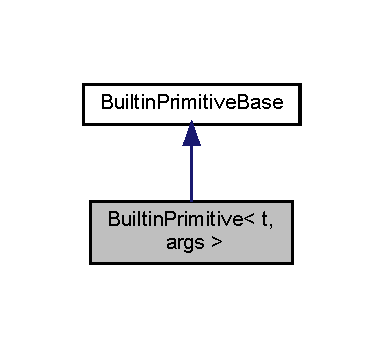
\includegraphics[width=184pt]{struct_builtin_primitive__inherit__graph}
\end{center}
\end{figure}


Collaboration diagram for Builtin\+Primitive$<$ t, args $>$\+:
\nopagebreak
\begin{figure}[H]
\begin{center}
\leavevmode
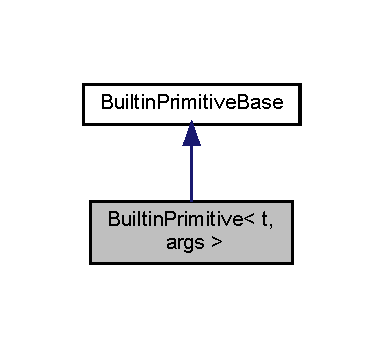
\includegraphics[width=184pt]{struct_builtin_primitive__coll__graph}
\end{center}
\end{figure}
\subsection*{Public Member Functions}
\begin{DoxyCompactItemize}
\item 
\hyperlink{struct_builtin_primitive_abad30dd239c26d27a2e6f1658aff9182}{Builtin\+Primitive} (std\+::string fmt, \hyperlink{_instruction_8h_af2fb7c87c5854c5733d7bb0506b06de7}{Builtin\+Op} o, double \+\_\+p)
\item 
{\footnotesize template$<$typename V , typename P , typename L $>$ }\\\hyperlink{_instruction_8h_a6202215407ab29590bb936ca2996cf64}{vmstatus\+\_\+t} \hyperlink{struct_builtin_primitive_a6403ebb7076028fa99751436768d6d81}{V\+M\+Scall} (V $\ast$vms, P $\ast$pool, L $\ast$loader)
\end{DoxyCompactItemize}
\subsection*{Public Attributes}
\begin{DoxyCompactItemize}
\item 
std\+::string \hyperlink{struct_builtin_primitive_aabf1561380f8c387cf3bf768f97bd4bd}{format}
\item 
\hyperlink{_instruction_8h_af2fb7c87c5854c5733d7bb0506b06de7}{Builtin\+Op} \hyperlink{struct_builtin_primitive_a996bd520f47a299728229774117d6188}{op}
\item 
double \hyperlink{struct_builtin_primitive_a1a8d8e62426c9454355412b80faf684c}{p}
\end{DoxyCompactItemize}


\subsection{Detailed Description}
\subsubsection*{template$<$typename t, typename... args$>$\newline
class Builtin\+Primitive$<$ t, args $>$}

\begin{DoxyAuthor}{Author}
piantado 
\end{DoxyAuthor}
\begin{DoxyDate}{Date}
06/05/20 
\end{DoxyDate}


\subsection{Constructor \& Destructor Documentation}
\mbox{\Hypertarget{struct_builtin_primitive_abad30dd239c26d27a2e6f1658aff9182}\label{struct_builtin_primitive_abad30dd239c26d27a2e6f1658aff9182}} 
\index{Builtin\+Primitive@{Builtin\+Primitive}!Builtin\+Primitive@{Builtin\+Primitive}}
\index{Builtin\+Primitive@{Builtin\+Primitive}!Builtin\+Primitive@{Builtin\+Primitive}}
\subsubsection{\texorpdfstring{Builtin\+Primitive()}{BuiltinPrimitive()}}
{\footnotesize\ttfamily template$<$typename t, typename... args$>$ \\
\hyperlink{struct_builtin_primitive}{Builtin\+Primitive}$<$ t, args $>$\+::\hyperlink{struct_builtin_primitive}{Builtin\+Primitive} (\begin{DoxyParamCaption}\item[{std\+::string}]{fmt,  }\item[{\hyperlink{_instruction_8h_af2fb7c87c5854c5733d7bb0506b06de7}{Builtin\+Op}}]{o,  }\item[{double}]{\+\_\+p }\end{DoxyParamCaption})\hspace{0.3cm}{\ttfamily [inline]}}



\subsection{Member Function Documentation}
\mbox{\Hypertarget{struct_builtin_primitive_a6403ebb7076028fa99751436768d6d81}\label{struct_builtin_primitive_a6403ebb7076028fa99751436768d6d81}} 
\index{Builtin\+Primitive@{Builtin\+Primitive}!V\+M\+Scall@{V\+M\+Scall}}
\index{V\+M\+Scall@{V\+M\+Scall}!Builtin\+Primitive@{Builtin\+Primitive}}
\subsubsection{\texorpdfstring{V\+M\+Scall()}{VMScall()}}
{\footnotesize\ttfamily template$<$typename t, typename... args$>$ \\
template$<$typename V , typename P , typename L $>$ \\
\hyperlink{_instruction_8h_a6202215407ab29590bb936ca2996cf64}{vmstatus\+\_\+t} \hyperlink{struct_builtin_primitive}{Builtin\+Primitive}$<$ t, args $>$\+::V\+M\+Scall (\begin{DoxyParamCaption}\item[{V $\ast$}]{vms,  }\item[{P $\ast$}]{pool,  }\item[{L $\ast$}]{loader }\end{DoxyParamCaption})\hspace{0.3cm}{\ttfamily [inline]}}



\subsection{Member Data Documentation}
\mbox{\Hypertarget{struct_builtin_primitive_aabf1561380f8c387cf3bf768f97bd4bd}\label{struct_builtin_primitive_aabf1561380f8c387cf3bf768f97bd4bd}} 
\index{Builtin\+Primitive@{Builtin\+Primitive}!format@{format}}
\index{format@{format}!Builtin\+Primitive@{Builtin\+Primitive}}
\subsubsection{\texorpdfstring{format}{format}}
{\footnotesize\ttfamily template$<$typename t, typename... args$>$ \\
std\+::string \hyperlink{struct_builtin_primitive}{Builtin\+Primitive}$<$ t, args $>$\+::format}

\mbox{\Hypertarget{struct_builtin_primitive_a996bd520f47a299728229774117d6188}\label{struct_builtin_primitive_a996bd520f47a299728229774117d6188}} 
\index{Builtin\+Primitive@{Builtin\+Primitive}!op@{op}}
\index{op@{op}!Builtin\+Primitive@{Builtin\+Primitive}}
\subsubsection{\texorpdfstring{op}{op}}
{\footnotesize\ttfamily template$<$typename t, typename... args$>$ \\
\hyperlink{_instruction_8h_af2fb7c87c5854c5733d7bb0506b06de7}{Builtin\+Op} \hyperlink{struct_builtin_primitive}{Builtin\+Primitive}$<$ t, args $>$\+::op}

\mbox{\Hypertarget{struct_builtin_primitive_a1a8d8e62426c9454355412b80faf684c}\label{struct_builtin_primitive_a1a8d8e62426c9454355412b80faf684c}} 
\index{Builtin\+Primitive@{Builtin\+Primitive}!p@{p}}
\index{p@{p}!Builtin\+Primitive@{Builtin\+Primitive}}
\subsubsection{\texorpdfstring{p}{p}}
{\footnotesize\ttfamily template$<$typename t, typename... args$>$ \\
double \hyperlink{struct_builtin_primitive}{Builtin\+Primitive}$<$ t, args $>$\+::p}



The documentation for this class was generated from the following file\+:\begin{DoxyCompactItemize}
\item 
src/\+Virtual\+Machine/\hyperlink{_builtins_8h}{Builtins.\+h}\end{DoxyCompactItemize}

\hypertarget{struct_builtin_primitive_base}{}\section{Builtin\+Primitive\+Base Struct Reference}
\label{struct_builtin_primitive_base}\index{Builtin\+Primitive\+Base@{Builtin\+Primitive\+Base}}


{\ttfamily \#include $<$Builtins.\+h$>$}



Inheritance diagram for Builtin\+Primitive\+Base\+:\nopagebreak
\begin{figure}[H]
\begin{center}
\leavevmode
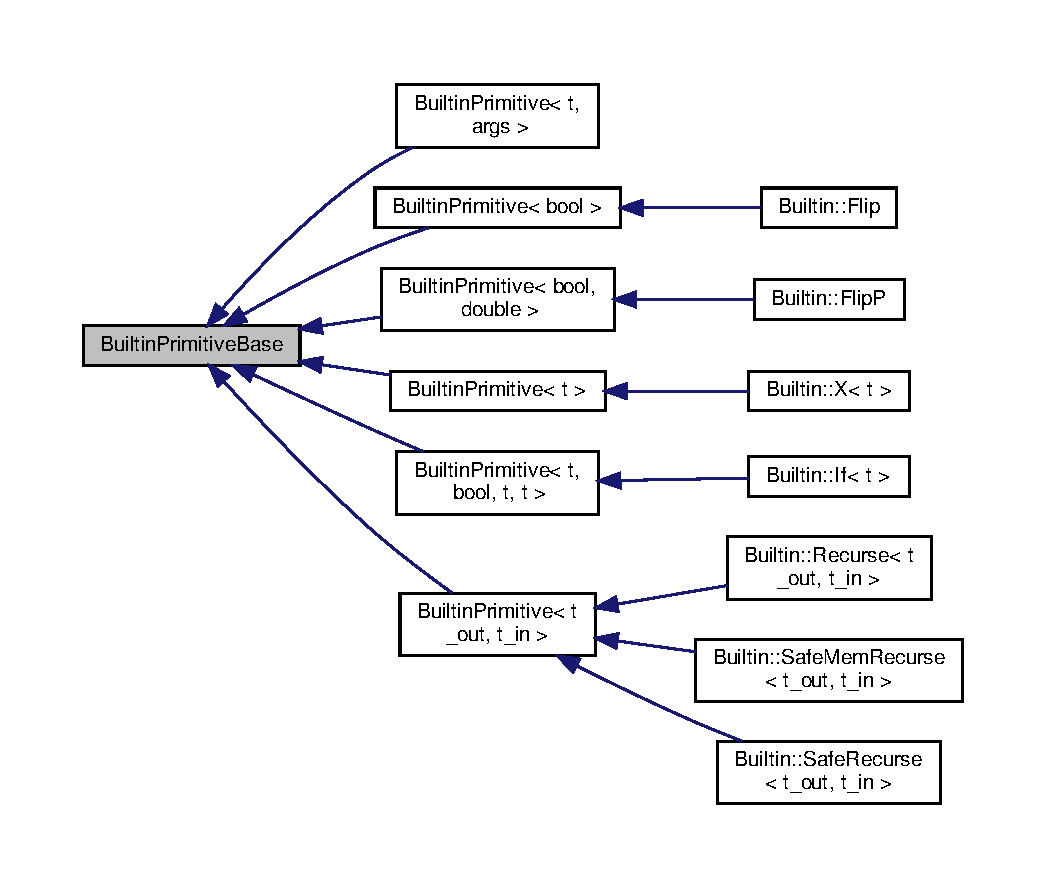
\includegraphics[width=350pt]{struct_builtin_primitive_base__inherit__graph}
\end{center}
\end{figure}


The documentation for this struct was generated from the following file\+:\begin{DoxyCompactItemize}
\item 
src/\+Virtual\+Machine/\hyperlink{_builtins_8h}{Builtins.\+h}\end{DoxyCompactItemize}

\hypertarget{class_builtin_primitive_root}{}\doxysection{Builtin\+Primitive\+Root Class Reference}
\label{class_builtin_primitive_root}\index{BuiltinPrimitiveRoot@{BuiltinPrimitiveRoot}}


{\ttfamily \#include $<$Builtins.\+h$>$}



\doxysubsection{Detailed Description}
\begin{DoxyAuthor}{Author}
piantado 
\end{DoxyAuthor}
\begin{DoxyDate}{Date}
06/05/20 
\end{DoxyDate}


The documentation for this class was generated from the following file\+:\begin{DoxyCompactItemize}
\item 
src/\+Virtual\+Machine/\mbox{\hyperlink{_builtins_8h}{Builtins.\+h}}\end{DoxyCompactItemize}

\hypertarget{class_chain_pool}{}\doxysection{Chain\+Pool$<$ H\+YP $>$ Class Template Reference}
\label{class_chain_pool}\index{ChainPool$<$ HYP $>$@{ChainPool$<$ HYP $>$}}


{\ttfamily \#include $<$Chain\+Pool.\+h$>$}



Inheritance diagram for Chain\+Pool$<$ H\+YP $>$\+:
\nopagebreak
\begin{figure}[H]
\begin{center}
\leavevmode
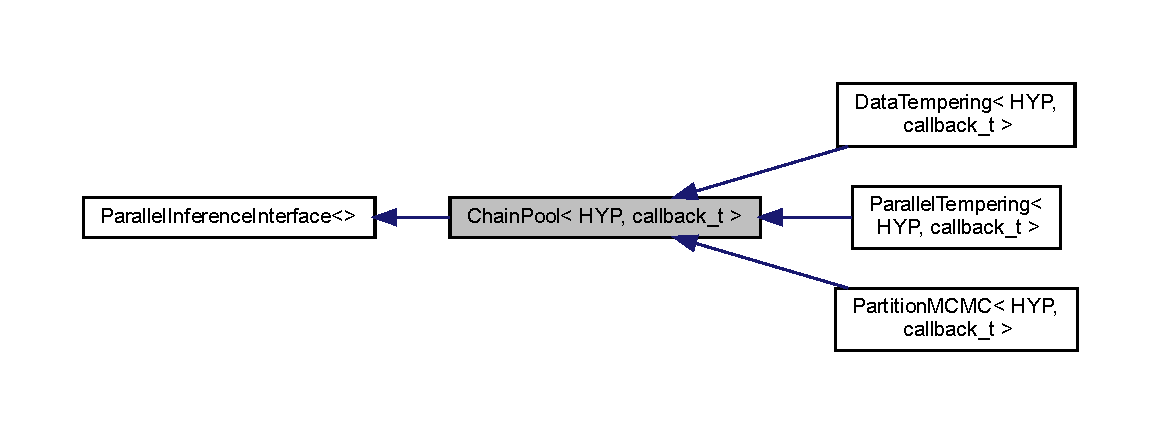
\includegraphics[width=350pt]{class_chain_pool__inherit__graph}
\end{center}
\end{figure}


Collaboration diagram for Chain\+Pool$<$ H\+YP $>$\+:
\nopagebreak
\begin{figure}[H]
\begin{center}
\leavevmode
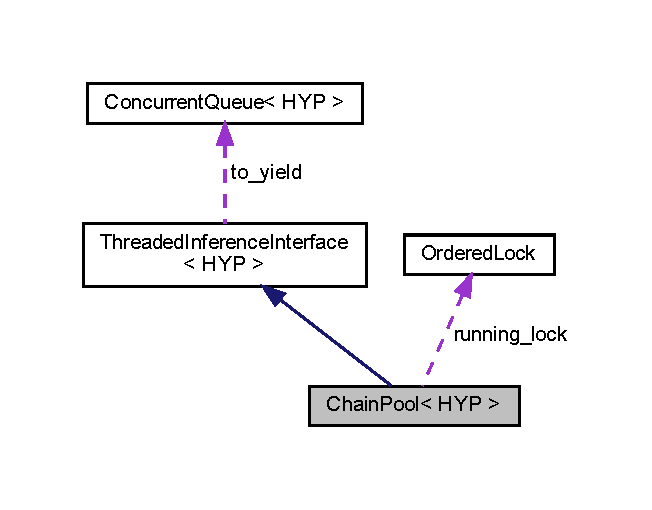
\includegraphics[width=339pt]{class_chain_pool__coll__graph}
\end{center}
\end{figure}
\doxysubsection*{Public Types}
\begin{DoxyCompactItemize}
\item 
enum \mbox{\hyperlink{class_chain_pool_a5a4f9d83b4492d9457a7db8581e25b75}{Running\+State}} \{ \mbox{\hyperlink{class_chain_pool_a5a4f9d83b4492d9457a7db8581e25b75a2baa69eafc7204f3bd8648eba580c489}{Running\+State\+::\+R\+E\+A\+DY}}, 
\mbox{\hyperlink{class_chain_pool_a5a4f9d83b4492d9457a7db8581e25b75a43491564ebcfd38568918efbd6e840fd}{Running\+State\+::\+R\+U\+N\+N\+I\+NG}}, 
\mbox{\hyperlink{class_chain_pool_a5a4f9d83b4492d9457a7db8581e25b75a2ba22e58ca17bb728d522bba36cf8350}{Running\+State\+::\+D\+O\+NE}}
 \}
\end{DoxyCompactItemize}
\doxysubsection*{Public Member Functions}
\begin{DoxyCompactItemize}
\item 
\mbox{\hyperlink{class_chain_pool_a553f1f3e478b29d721b596854a2e6f52}{Chain\+Pool}} ()
\item 
\mbox{\hyperlink{class_chain_pool_a203b5e60aa34764edbab67f27d2c413b}{Chain\+Pool}} (H\+YP \&h0, typename H\+Y\+P\+::data\+\_\+t $\ast$d, size\+\_\+t n)
\item 
void \mbox{\hyperlink{class_chain_pool_a6c186d7addcd0e1ab0733aae3a760a47}{set\+\_\+data}} (typename H\+Y\+P\+::data\+\_\+t $\ast$d, bool recompute=true)
\begin{DoxyCompactList}\small\item\em Set this data. \end{DoxyCompactList}\item 
size\+\_\+t \mbox{\hyperlink{class_chain_pool_aeec4366901f693ebe3a4275ac00dde2a}{nchains}} () const
\item 
void \mbox{\hyperlink{class_chain_pool_a38e61af5e8d4c0399ac0a30e2a0e18ce}{print}} (std\+::string prefix) const
\item 
\mbox{\hyperlink{_coroutines_8h_ab06a612c41229b9582ada8655001e2b0}{generator}}$<$ H\+YP \& $>$ \mbox{\hyperlink{class_chain_pool_a84ad82009e98da528a9ab9aa97b6e81c}{run\+\_\+thread}} (\mbox{\hyperlink{struct_control}{Control}} \&ctl) override
\begin{DoxyCompactList}\small\item\em This run helper is called internally by multiple different threads, and runs a given pool. \end{DoxyCompactList}\end{DoxyCompactItemize}
\doxysubsection*{Public Attributes}
\begin{DoxyCompactItemize}
\item 
std\+::vector$<$ \mbox{\hyperlink{class_m_c_m_c_chain}{M\+C\+M\+C\+Chain}}$<$ H\+YP $>$ $>$ \mbox{\hyperlink{class_chain_pool_aca174138c188771e02ef6cb2e0e9d42b}{pool}}
\item 
unsigned long \mbox{\hyperlink{class_chain_pool_a327b47178f3753da10661b08cd60b406}{steps\+\_\+before\+\_\+change}} = 100
\item 
std\+::vector$<$ \mbox{\hyperlink{class_chain_pool_a5a4f9d83b4492d9457a7db8581e25b75}{Running\+State}} $>$ \mbox{\hyperlink{class_chain_pool_a5bba2491596087935cea0fe02c7af423}{running}}
\item 
\mbox{\hyperlink{class_ordered_lock}{Ordered\+Lock}} \mbox{\hyperlink{class_chain_pool_aa66dd89ec348fab23911f3f8c91123d1}{running\+\_\+lock}}
\end{DoxyCompactItemize}


\doxysubsection{Detailed Description}
\subsubsection*{template$<$typename H\+YP$>$\newline
class Chain\+Pool$<$ H\+Y\+P $>$}

\begin{DoxyAuthor}{Author}
steven piantadosi 
\end{DoxyAuthor}
\begin{DoxyDate}{Date}
29/01/20 
\end{DoxyDate}


\doxysubsection{Member Enumeration Documentation}
\mbox{\Hypertarget{class_chain_pool_a5a4f9d83b4492d9457a7db8581e25b75}\label{class_chain_pool_a5a4f9d83b4492d9457a7db8581e25b75}} 
\index{ChainPool$<$ HYP $>$@{ChainPool$<$ HYP $>$}!RunningState@{RunningState}}
\index{RunningState@{RunningState}!ChainPool$<$ HYP $>$@{ChainPool$<$ HYP $>$}}
\doxysubsubsection{\texorpdfstring{RunningState}{RunningState}}
{\footnotesize\ttfamily template$<$typename H\+YP $>$ \\
enum \mbox{\hyperlink{class_chain_pool_a5a4f9d83b4492d9457a7db8581e25b75}{Chain\+Pool\+::\+Running\+State}}\hspace{0.3cm}{\ttfamily [strong]}}

\begin{DoxyEnumFields}{Enumerator}
\raisebox{\heightof{T}}[0pt][0pt]{\index{READY@{READY}!ChainPool$<$ HYP $>$@{ChainPool$<$ HYP $>$}}\index{ChainPool$<$ HYP $>$@{ChainPool$<$ HYP $>$}!READY@{READY}}}\mbox{\Hypertarget{class_chain_pool_a5a4f9d83b4492d9457a7db8581e25b75a2baa69eafc7204f3bd8648eba580c489}\label{class_chain_pool_a5a4f9d83b4492d9457a7db8581e25b75a2baa69eafc7204f3bd8648eba580c489}} 
R\+E\+A\+DY&\\
\hline

\raisebox{\heightof{T}}[0pt][0pt]{\index{RUNNING@{RUNNING}!ChainPool$<$ HYP $>$@{ChainPool$<$ HYP $>$}}\index{ChainPool$<$ HYP $>$@{ChainPool$<$ HYP $>$}!RUNNING@{RUNNING}}}\mbox{\Hypertarget{class_chain_pool_a5a4f9d83b4492d9457a7db8581e25b75a43491564ebcfd38568918efbd6e840fd}\label{class_chain_pool_a5a4f9d83b4492d9457a7db8581e25b75a43491564ebcfd38568918efbd6e840fd}} 
R\+U\+N\+N\+I\+NG&\\
\hline

\raisebox{\heightof{T}}[0pt][0pt]{\index{DONE@{DONE}!ChainPool$<$ HYP $>$@{ChainPool$<$ HYP $>$}}\index{ChainPool$<$ HYP $>$@{ChainPool$<$ HYP $>$}!DONE@{DONE}}}\mbox{\Hypertarget{class_chain_pool_a5a4f9d83b4492d9457a7db8581e25b75a2ba22e58ca17bb728d522bba36cf8350}\label{class_chain_pool_a5a4f9d83b4492d9457a7db8581e25b75a2ba22e58ca17bb728d522bba36cf8350}} 
D\+O\+NE&\\
\hline

\end{DoxyEnumFields}


\doxysubsection{Constructor \& Destructor Documentation}
\mbox{\Hypertarget{class_chain_pool_a553f1f3e478b29d721b596854a2e6f52}\label{class_chain_pool_a553f1f3e478b29d721b596854a2e6f52}} 
\index{ChainPool$<$ HYP $>$@{ChainPool$<$ HYP $>$}!ChainPool@{ChainPool}}
\index{ChainPool@{ChainPool}!ChainPool$<$ HYP $>$@{ChainPool$<$ HYP $>$}}
\doxysubsubsection{\texorpdfstring{ChainPool()}{ChainPool()}\hspace{0.1cm}{\footnotesize\ttfamily [1/2]}}
{\footnotesize\ttfamily template$<$typename H\+YP $>$ \\
\mbox{\hyperlink{class_chain_pool}{Chain\+Pool}}$<$ H\+YP $>$\+::\mbox{\hyperlink{class_chain_pool}{Chain\+Pool}} (\begin{DoxyParamCaption}{ }\end{DoxyParamCaption})\hspace{0.3cm}{\ttfamily [inline]}}

\mbox{\Hypertarget{class_chain_pool_a203b5e60aa34764edbab67f27d2c413b}\label{class_chain_pool_a203b5e60aa34764edbab67f27d2c413b}} 
\index{ChainPool$<$ HYP $>$@{ChainPool$<$ HYP $>$}!ChainPool@{ChainPool}}
\index{ChainPool@{ChainPool}!ChainPool$<$ HYP $>$@{ChainPool$<$ HYP $>$}}
\doxysubsubsection{\texorpdfstring{ChainPool()}{ChainPool()}\hspace{0.1cm}{\footnotesize\ttfamily [2/2]}}
{\footnotesize\ttfamily template$<$typename H\+YP $>$ \\
\mbox{\hyperlink{class_chain_pool}{Chain\+Pool}}$<$ H\+YP $>$\+::\mbox{\hyperlink{class_chain_pool}{Chain\+Pool}} (\begin{DoxyParamCaption}\item[{H\+YP \&}]{h0,  }\item[{typename H\+Y\+P\+::data\+\_\+t $\ast$}]{d,  }\item[{size\+\_\+t}]{n }\end{DoxyParamCaption})\hspace{0.3cm}{\ttfamily [inline]}}



\doxysubsection{Member Function Documentation}
\mbox{\Hypertarget{class_chain_pool_aeec4366901f693ebe3a4275ac00dde2a}\label{class_chain_pool_aeec4366901f693ebe3a4275ac00dde2a}} 
\index{ChainPool$<$ HYP $>$@{ChainPool$<$ HYP $>$}!nchains@{nchains}}
\index{nchains@{nchains}!ChainPool$<$ HYP $>$@{ChainPool$<$ HYP $>$}}
\doxysubsubsection{\texorpdfstring{nchains()}{nchains()}}
{\footnotesize\ttfamily template$<$typename H\+YP $>$ \\
size\+\_\+t \mbox{\hyperlink{class_chain_pool}{Chain\+Pool}}$<$ H\+YP $>$\+::nchains (\begin{DoxyParamCaption}{ }\end{DoxyParamCaption}) const\hspace{0.3cm}{\ttfamily [inline]}}

\mbox{\Hypertarget{class_chain_pool_a38e61af5e8d4c0399ac0a30e2a0e18ce}\label{class_chain_pool_a38e61af5e8d4c0399ac0a30e2a0e18ce}} 
\index{ChainPool$<$ HYP $>$@{ChainPool$<$ HYP $>$}!print@{print}}
\index{print@{print}!ChainPool$<$ HYP $>$@{ChainPool$<$ HYP $>$}}
\doxysubsubsection{\texorpdfstring{print()}{print()}}
{\footnotesize\ttfamily template$<$typename H\+YP $>$ \\
void \mbox{\hyperlink{class_chain_pool}{Chain\+Pool}}$<$ H\+YP $>$\+::\mbox{\hyperlink{structprint}{print}} (\begin{DoxyParamCaption}\item[{std\+::string}]{prefix }\end{DoxyParamCaption}) const\hspace{0.3cm}{\ttfamily [inline]}}

\mbox{\Hypertarget{class_chain_pool_a84ad82009e98da528a9ab9aa97b6e81c}\label{class_chain_pool_a84ad82009e98da528a9ab9aa97b6e81c}} 
\index{ChainPool$<$ HYP $>$@{ChainPool$<$ HYP $>$}!run\_thread@{run\_thread}}
\index{run\_thread@{run\_thread}!ChainPool$<$ HYP $>$@{ChainPool$<$ HYP $>$}}
\doxysubsubsection{\texorpdfstring{run\_thread()}{run\_thread()}}
{\footnotesize\ttfamily template$<$typename H\+YP $>$ \\
\mbox{\hyperlink{_coroutines_8h_ab06a612c41229b9582ada8655001e2b0}{generator}}$<$H\+YP\&$>$ \mbox{\hyperlink{class_chain_pool}{Chain\+Pool}}$<$ H\+YP $>$\+::run\+\_\+thread (\begin{DoxyParamCaption}\item[{\mbox{\hyperlink{struct_control}{Control}} \&}]{ctl }\end{DoxyParamCaption})\hspace{0.3cm}{\ttfamily [inline]}, {\ttfamily [override]}}



This run helper is called internally by multiple different threads, and runs a given pool. 


\begin{DoxyParams}{Parameters}
{\em ctl} & \\
\hline
\end{DoxyParams}
figure out how many steps to run\mbox{\Hypertarget{class_chain_pool_a6c186d7addcd0e1ab0733aae3a760a47}\label{class_chain_pool_a6c186d7addcd0e1ab0733aae3a760a47}} 
\index{ChainPool$<$ HYP $>$@{ChainPool$<$ HYP $>$}!set\_data@{set\_data}}
\index{set\_data@{set\_data}!ChainPool$<$ HYP $>$@{ChainPool$<$ HYP $>$}}
\doxysubsubsection{\texorpdfstring{set\_data()}{set\_data()}}
{\footnotesize\ttfamily template$<$typename H\+YP $>$ \\
void \mbox{\hyperlink{class_chain_pool}{Chain\+Pool}}$<$ H\+YP $>$\+::set\+\_\+data (\begin{DoxyParamCaption}\item[{typename H\+Y\+P\+::data\+\_\+t $\ast$}]{d,  }\item[{bool}]{recompute = {\ttfamily true} }\end{DoxyParamCaption})\hspace{0.3cm}{\ttfamily [inline]}}



Set this data. 


\begin{DoxyParams}{Parameters}
{\em d} & -- what data to set \\
\hline
{\em recompute} & -- should I recompute all of the posteriors? \\
\hline
\end{DoxyParams}


\doxysubsection{Member Data Documentation}
\mbox{\Hypertarget{class_chain_pool_aca174138c188771e02ef6cb2e0e9d42b}\label{class_chain_pool_aca174138c188771e02ef6cb2e0e9d42b}} 
\index{ChainPool$<$ HYP $>$@{ChainPool$<$ HYP $>$}!pool@{pool}}
\index{pool@{pool}!ChainPool$<$ HYP $>$@{ChainPool$<$ HYP $>$}}
\doxysubsubsection{\texorpdfstring{pool}{pool}}
{\footnotesize\ttfamily template$<$typename H\+YP $>$ \\
std\+::vector$<$\mbox{\hyperlink{class_m_c_m_c_chain}{M\+C\+M\+C\+Chain}}$<$H\+YP$>$ $>$ \mbox{\hyperlink{class_chain_pool}{Chain\+Pool}}$<$ H\+YP $>$\+::pool}

\mbox{\Hypertarget{class_chain_pool_a5bba2491596087935cea0fe02c7af423}\label{class_chain_pool_a5bba2491596087935cea0fe02c7af423}} 
\index{ChainPool$<$ HYP $>$@{ChainPool$<$ HYP $>$}!running@{running}}
\index{running@{running}!ChainPool$<$ HYP $>$@{ChainPool$<$ HYP $>$}}
\doxysubsubsection{\texorpdfstring{running}{running}}
{\footnotesize\ttfamily template$<$typename H\+YP $>$ \\
std\+::vector$<$\mbox{\hyperlink{class_chain_pool_a5a4f9d83b4492d9457a7db8581e25b75}{Running\+State}}$>$ \mbox{\hyperlink{class_chain_pool}{Chain\+Pool}}$<$ H\+YP $>$\+::running}

\mbox{\Hypertarget{class_chain_pool_aa66dd89ec348fab23911f3f8c91123d1}\label{class_chain_pool_aa66dd89ec348fab23911f3f8c91123d1}} 
\index{ChainPool$<$ HYP $>$@{ChainPool$<$ HYP $>$}!running\_lock@{running\_lock}}
\index{running\_lock@{running\_lock}!ChainPool$<$ HYP $>$@{ChainPool$<$ HYP $>$}}
\doxysubsubsection{\texorpdfstring{running\_lock}{running\_lock}}
{\footnotesize\ttfamily template$<$typename H\+YP $>$ \\
\mbox{\hyperlink{class_ordered_lock}{Ordered\+Lock}} \mbox{\hyperlink{class_chain_pool}{Chain\+Pool}}$<$ H\+YP $>$\+::running\+\_\+lock}

\mbox{\Hypertarget{class_chain_pool_a327b47178f3753da10661b08cd60b406}\label{class_chain_pool_a327b47178f3753da10661b08cd60b406}} 
\index{ChainPool$<$ HYP $>$@{ChainPool$<$ HYP $>$}!steps\_before\_change@{steps\_before\_change}}
\index{steps\_before\_change@{steps\_before\_change}!ChainPool$<$ HYP $>$@{ChainPool$<$ HYP $>$}}
\doxysubsubsection{\texorpdfstring{steps\_before\_change}{steps\_before\_change}}
{\footnotesize\ttfamily template$<$typename H\+YP $>$ \\
unsigned long \mbox{\hyperlink{class_chain_pool}{Chain\+Pool}}$<$ H\+YP $>$\+::steps\+\_\+before\+\_\+change = 100}



The documentation for this class was generated from the following file\+:\begin{DoxyCompactItemize}
\item 
src/\+Inference/\+M\+C\+M\+C/\mbox{\hyperlink{_chain_pool_8h}{Chain\+Pool.\+h}}\end{DoxyCompactItemize}

\hypertarget{classcheck_builtins_are_last}{}\section{check\+Builtins\+Are\+Last Class Reference}
\label{classcheck_builtins_are_last}\index{check\+Builtins\+Are\+Last@{check\+Builtins\+Are\+Last}}


{\ttfamily \#include $<$Builtins.\+h$>$}



\subsection{Detailed Description}
\begin{DoxyAuthor}{Author}
piantado 
\end{DoxyAuthor}
\begin{DoxyDate}{Date}
06/05/20 
\end{DoxyDate}


The documentation for this class was generated from the following file\+:\begin{DoxyCompactItemize}
\item 
src/\+Virtual\+Machine/\hyperlink{_builtins_8h}{Builtins.\+h}\end{DoxyCompactItemize}

\hypertarget{struct_check_reference_is_first}{}\section{Check\+Reference\+Is\+First$<$ T, Types $>$ Class Template Reference}
\label{struct_check_reference_is_first}\index{Check\+Reference\+Is\+First$<$ T, Types $>$@{Check\+Reference\+Is\+First$<$ T, Types $>$}}


{\ttfamily \#include $<$Primitives.\+h$>$}

\subsection*{Static Public Attributes}
\begin{DoxyCompactItemize}
\item 
static const bool \hyperlink{struct_check_reference_is_first_a0b4db809c2e3980d79ba182e7da8d50f}{value} = (\hyperlink{struct_count_references}{Count\+References}$<$Types...$>$\+::value == 0)
\end{DoxyCompactItemize}


\subsection{Detailed Description}
\subsubsection*{template$<$class T, class... Types$>$\newline
class Check\+Reference\+Is\+First$<$ T, Types $>$}

\begin{DoxyAuthor}{Author}
piantado 
\end{DoxyAuthor}
\begin{DoxyDate}{Date}
07/05/20 
\end{DoxyDate}


\subsection{Member Data Documentation}
\mbox{\Hypertarget{struct_check_reference_is_first_a0b4db809c2e3980d79ba182e7da8d50f}\label{struct_check_reference_is_first_a0b4db809c2e3980d79ba182e7da8d50f}} 
\index{Check\+Reference\+Is\+First@{Check\+Reference\+Is\+First}!value@{value}}
\index{value@{value}!Check\+Reference\+Is\+First@{Check\+Reference\+Is\+First}}
\subsubsection{\texorpdfstring{value}{value}}
{\footnotesize\ttfamily template$<$class T , class... Types$>$ \\
const bool \hyperlink{struct_check_reference_is_first}{Check\+Reference\+Is\+First}$<$ T, Types $>$\+::value = (\hyperlink{struct_count_references}{Count\+References}$<$Types...$>$\+::value == 0)\hspace{0.3cm}{\ttfamily [static]}}



The documentation for this class was generated from the following file\+:\begin{DoxyCompactItemize}
\item 
src/\+Virtual\+Machine/\hyperlink{_primitives_8h}{Primitives.\+h}\end{DoxyCompactItemize}

\hypertarget{struct_check_reference_is_first_3_01_t_01_4}{}\doxysection{Check\+Reference\+Is\+First$<$ T $>$ Struct Template Reference}
\label{struct_check_reference_is_first_3_01_t_01_4}\index{CheckReferenceIsFirst$<$ T $>$@{CheckReferenceIsFirst$<$ T $>$}}


{\ttfamily \#include $<$Primitives.\+h$>$}

\doxysubsection*{Static Public Attributes}
\begin{DoxyCompactItemize}
\item 
static const bool \mbox{\hyperlink{struct_check_reference_is_first_3_01_t_01_4_aa06e980782a7c07ee58484ee20974f5c}{value}} = true
\end{DoxyCompactItemize}


\doxysubsection{Member Data Documentation}
\mbox{\Hypertarget{struct_check_reference_is_first_3_01_t_01_4_aa06e980782a7c07ee58484ee20974f5c}\label{struct_check_reference_is_first_3_01_t_01_4_aa06e980782a7c07ee58484ee20974f5c}} 
\index{CheckReferenceIsFirst$<$ T $>$@{CheckReferenceIsFirst$<$ T $>$}!value@{value}}
\index{value@{value}!CheckReferenceIsFirst$<$ T $>$@{CheckReferenceIsFirst$<$ T $>$}}
\doxysubsubsection{\texorpdfstring{value}{value}}
{\footnotesize\ttfamily template$<$class T $>$ \\
const bool \mbox{\hyperlink{struct_check_reference_is_first}{Check\+Reference\+Is\+First}}$<$ T $>$\+::value = true\hspace{0.3cm}{\ttfamily [static]}}



The documentation for this struct was generated from the following file\+:\begin{DoxyCompactItemize}
\item 
src/\+Virtual\+Machine/\mbox{\hyperlink{_primitives_8h}{Primitives.\+h}}\end{DoxyCompactItemize}

\hypertarget{struct_combinators_1_1_c_l}{}\doxysection{Combinators\+::CL Struct Reference}
\label{struct_combinators_1_1_c_l}\index{Combinators::CL@{Combinators::CL}}


{\ttfamily \#include $<$Combinators.\+h$>$}

\doxysubsection*{Public Member Functions}
\begin{DoxyCompactItemize}
\item 
bool \mbox{\hyperlink{struct_combinators_1_1_c_l_a81f3673cc2acbaaa9194c84352905bce}{operator$<$}} (const \mbox{\hyperlink{struct_combinators_1_1_c_l}{CL}} \&other) const
\end{DoxyCompactItemize}


\doxysubsection{Member Function Documentation}
\mbox{\Hypertarget{struct_combinators_1_1_c_l_a81f3673cc2acbaaa9194c84352905bce}\label{struct_combinators_1_1_c_l_a81f3673cc2acbaaa9194c84352905bce}} 
\index{Combinators::CL@{Combinators::CL}!operator$<$@{operator$<$}}
\index{operator$<$@{operator$<$}!Combinators::CL@{Combinators::CL}}
\doxysubsubsection{\texorpdfstring{operator$<$()}{operator<()}}
{\footnotesize\ttfamily bool Combinators\+::\+C\+L\+::operator$<$ (\begin{DoxyParamCaption}\item[{const \mbox{\hyperlink{struct_combinators_1_1_c_l}{CL}} \&}]{other }\end{DoxyParamCaption}) const\hspace{0.3cm}{\ttfamily [inline]}}



The documentation for this struct was generated from the following file\+:\begin{DoxyCompactItemize}
\item 
src/\mbox{\hyperlink{_combinators_8h}{Combinators.\+h}}\end{DoxyCompactItemize}

\hypertarget{struct_control}{}\doxysection{Control Class Reference}
\label{struct_control}\index{Control@{Control}}


{\ttfamily \#include $<$Control.\+h$>$}

\doxysubsection*{Public Member Functions}
\begin{DoxyCompactItemize}
\item 
\mbox{\hyperlink{struct_control_a1403ae58ef8c681793bd3d94b3f3e704}{Control}} (unsigned long st=\mbox{\hyperlink{namespace_fleet_args_a0cabfaa21ab6740518265b14df5948c7}{Fleet\+Args\+::steps}}, unsigned long t=\mbox{\hyperlink{namespace_fleet_args_a094bc8aa2836c57906405cde03d24fc6}{Fleet\+Args\+::runtime}}, size\+\_\+t thr=\mbox{\hyperlink{namespace_fleet_args_a90ee834a1804002baec2366daeda54a5}{Fleet\+Args\+::nthreads}}, unsigned long bu=\mbox{\hyperlink{namespace_fleet_args_a7dc1ce66659f9dc509b370d5660582e8}{Fleet\+Args\+::burn}}, unsigned long re=\mbox{\hyperlink{namespace_fleet_args_af0c62e1528330a5fb0ba9f01082aa823}{Fleet\+Args\+::restart}}, unsigned long th=\mbox{\hyperlink{namespace_fleet_args_add2603eb3b9b47d79684e1a12bcca2aa}{Fleet\+Args\+::thin}}, unsigned long pr=\mbox{\hyperlink{namespace_fleet_args_acf2f80bb2810cea3b3eeef0c4b0edf03}{Fleet\+Args\+::print}})
\item 
void \mbox{\hyperlink{struct_control_a933994a3524f2f6d7ef0a17086e7cf66}{start}} ()
\item 
bool \mbox{\hyperlink{struct_control_a9217475a8ad619e7360524ae49c559a7}{running}} ()
\end{DoxyCompactItemize}
\doxysubsection*{Public Attributes}
\begin{DoxyCompactItemize}
\item 
unsigned long \mbox{\hyperlink{struct_control_af4bd5a6c779079b5e921b4df40760266}{steps}}
\item 
time\+\_\+ms \mbox{\hyperlink{struct_control_ae14b7e8a0d59a10d5fb7d000707ed4b9}{runtime}}
\item 
size\+\_\+t \mbox{\hyperlink{struct_control_a7c7748be70415c187e9cfd8124ab711b}{nthreads}}
\item 
unsigned long \mbox{\hyperlink{struct_control_acb1e669784385d64b9f840674a3e08c1}{burn}}
\item 
unsigned long \mbox{\hyperlink{struct_control_acd75b8aa48fdb33f063bae7469a9721b}{restart}}
\item 
unsigned long \mbox{\hyperlink{struct_control_a08030350e86fd21411599690892e31a8}{thin}}
\item 
unsigned long \mbox{\hyperlink{struct_control_a508fb30a9e74771b84bb846bcd6f2f2a}{print}}
\item 
timept \mbox{\hyperlink{struct_control_ad3c2691a66705880844f467cf5da8aab}{start\+\_\+time}}
\item 
unsigned long \mbox{\hyperlink{struct_control_a4a1867401c3e89aecaf14949521ed247}{done\+\_\+steps}}
\item 
bool \mbox{\hyperlink{struct_control_a3a1856c582efd2a6a1b8f40351038d0c}{break\+\_\+\+C\+T\+R\+LC}}
\end{DoxyCompactItemize}


\doxysubsection{Detailed Description}
\begin{DoxyAuthor}{Author}
Steven Piantadosi 
\end{DoxyAuthor}
\begin{DoxyDate}{Date}
17/08/20 
\end{DoxyDate}


\doxysubsection{Constructor \& Destructor Documentation}
\mbox{\Hypertarget{struct_control_a1403ae58ef8c681793bd3d94b3f3e704}\label{struct_control_a1403ae58ef8c681793bd3d94b3f3e704}} 
\index{Control@{Control}!Control@{Control}}
\index{Control@{Control}!Control@{Control}}
\doxysubsubsection{\texorpdfstring{Control()}{Control()}}
{\footnotesize\ttfamily Control\+::\+Control (\begin{DoxyParamCaption}\item[{unsigned long}]{st = {\ttfamily \mbox{\hyperlink{namespace_fleet_args_a0cabfaa21ab6740518265b14df5948c7}{Fleet\+Args\+::steps}}},  }\item[{unsigned long}]{t = {\ttfamily \mbox{\hyperlink{namespace_fleet_args_a094bc8aa2836c57906405cde03d24fc6}{Fleet\+Args\+::runtime}}},  }\item[{size\+\_\+t}]{thr = {\ttfamily \mbox{\hyperlink{namespace_fleet_args_a90ee834a1804002baec2366daeda54a5}{Fleet\+Args\+::nthreads}}},  }\item[{unsigned long}]{bu = {\ttfamily \mbox{\hyperlink{namespace_fleet_args_a7dc1ce66659f9dc509b370d5660582e8}{Fleet\+Args\+::burn}}},  }\item[{unsigned long}]{re = {\ttfamily \mbox{\hyperlink{namespace_fleet_args_af0c62e1528330a5fb0ba9f01082aa823}{Fleet\+Args\+::restart}}},  }\item[{unsigned long}]{th = {\ttfamily \mbox{\hyperlink{namespace_fleet_args_add2603eb3b9b47d79684e1a12bcca2aa}{Fleet\+Args\+::thin}}},  }\item[{unsigned long}]{pr = {\ttfamily \mbox{\hyperlink{namespace_fleet_args_acf2f80bb2810cea3b3eeef0c4b0edf03}{Fleet\+Args\+::print}}} }\end{DoxyParamCaption})\hspace{0.3cm}{\ttfamily [inline]}}



\doxysubsection{Member Function Documentation}
\mbox{\Hypertarget{struct_control_a9217475a8ad619e7360524ae49c559a7}\label{struct_control_a9217475a8ad619e7360524ae49c559a7}} 
\index{Control@{Control}!running@{running}}
\index{running@{running}!Control@{Control}}
\doxysubsubsection{\texorpdfstring{running()}{running()}}
{\footnotesize\ttfamily bool Control\+::running (\begin{DoxyParamCaption}{ }\end{DoxyParamCaption})\hspace{0.3cm}{\ttfamily [inline]}}

Check if we are currently running. \begin{DoxyReturn}{Returns}

\end{DoxyReturn}
\mbox{\Hypertarget{struct_control_a933994a3524f2f6d7ef0a17086e7cf66}\label{struct_control_a933994a3524f2f6d7ef0a17086e7cf66}} 
\index{Control@{Control}!start@{start}}
\index{start@{start}!Control@{Control}}
\doxysubsubsection{\texorpdfstring{start()}{start()}}
{\footnotesize\ttfamily void Control\+::start (\begin{DoxyParamCaption}{ }\end{DoxyParamCaption})\hspace{0.3cm}{\ttfamily [inline]}}

Start running

\doxysubsection{Member Data Documentation}
\mbox{\Hypertarget{struct_control_a3a1856c582efd2a6a1b8f40351038d0c}\label{struct_control_a3a1856c582efd2a6a1b8f40351038d0c}} 
\index{Control@{Control}!break\_CTRLC@{break\_CTRLC}}
\index{break\_CTRLC@{break\_CTRLC}!Control@{Control}}
\doxysubsubsection{\texorpdfstring{break\_CTRLC}{break\_CTRLC}}
{\footnotesize\ttfamily bool Control\+::break\+\_\+\+C\+T\+R\+LC}

\mbox{\Hypertarget{struct_control_acb1e669784385d64b9f840674a3e08c1}\label{struct_control_acb1e669784385d64b9f840674a3e08c1}} 
\index{Control@{Control}!burn@{burn}}
\index{burn@{burn}!Control@{Control}}
\doxysubsubsection{\texorpdfstring{burn}{burn}}
{\footnotesize\ttfamily unsigned long Control\+::burn}

\mbox{\Hypertarget{struct_control_a4a1867401c3e89aecaf14949521ed247}\label{struct_control_a4a1867401c3e89aecaf14949521ed247}} 
\index{Control@{Control}!done\_steps@{done\_steps}}
\index{done\_steps@{done\_steps}!Control@{Control}}
\doxysubsubsection{\texorpdfstring{done\_steps}{done\_steps}}
{\footnotesize\ttfamily unsigned long Control\+::done\+\_\+steps}

\mbox{\Hypertarget{struct_control_a7c7748be70415c187e9cfd8124ab711b}\label{struct_control_a7c7748be70415c187e9cfd8124ab711b}} 
\index{Control@{Control}!nthreads@{nthreads}}
\index{nthreads@{nthreads}!Control@{Control}}
\doxysubsubsection{\texorpdfstring{nthreads}{nthreads}}
{\footnotesize\ttfamily size\+\_\+t Control\+::nthreads}

\mbox{\Hypertarget{struct_control_a508fb30a9e74771b84bb846bcd6f2f2a}\label{struct_control_a508fb30a9e74771b84bb846bcd6f2f2a}} 
\index{Control@{Control}!print@{print}}
\index{print@{print}!Control@{Control}}
\doxysubsubsection{\texorpdfstring{print}{print}}
{\footnotesize\ttfamily unsigned long Control\+::print}

\mbox{\Hypertarget{struct_control_acd75b8aa48fdb33f063bae7469a9721b}\label{struct_control_acd75b8aa48fdb33f063bae7469a9721b}} 
\index{Control@{Control}!restart@{restart}}
\index{restart@{restart}!Control@{Control}}
\doxysubsubsection{\texorpdfstring{restart}{restart}}
{\footnotesize\ttfamily unsigned long Control\+::restart}

\mbox{\Hypertarget{struct_control_ae14b7e8a0d59a10d5fb7d000707ed4b9}\label{struct_control_ae14b7e8a0d59a10d5fb7d000707ed4b9}} 
\index{Control@{Control}!runtime@{runtime}}
\index{runtime@{runtime}!Control@{Control}}
\doxysubsubsection{\texorpdfstring{runtime}{runtime}}
{\footnotesize\ttfamily time\+\_\+ms Control\+::runtime}

\mbox{\Hypertarget{struct_control_ad3c2691a66705880844f467cf5da8aab}\label{struct_control_ad3c2691a66705880844f467cf5da8aab}} 
\index{Control@{Control}!start\_time@{start\_time}}
\index{start\_time@{start\_time}!Control@{Control}}
\doxysubsubsection{\texorpdfstring{start\_time}{start\_time}}
{\footnotesize\ttfamily timept Control\+::start\+\_\+time}

\mbox{\Hypertarget{struct_control_af4bd5a6c779079b5e921b4df40760266}\label{struct_control_af4bd5a6c779079b5e921b4df40760266}} 
\index{Control@{Control}!steps@{steps}}
\index{steps@{steps}!Control@{Control}}
\doxysubsubsection{\texorpdfstring{steps}{steps}}
{\footnotesize\ttfamily unsigned long Control\+::steps}

\mbox{\Hypertarget{struct_control_a08030350e86fd21411599690892e31a8}\label{struct_control_a08030350e86fd21411599690892e31a8}} 
\index{Control@{Control}!thin@{thin}}
\index{thin@{thin}!Control@{Control}}
\doxysubsubsection{\texorpdfstring{thin}{thin}}
{\footnotesize\ttfamily unsigned long Control\+::thin}



The documentation for this class was generated from the following file\+:\begin{DoxyCompactItemize}
\item 
src/\+Inference/\mbox{\hyperlink{_control_8h}{Control.\+h}}\end{DoxyCompactItemize}

\hypertarget{struct_count_references}{}\doxysection{Count\+References$<$ T, Types $>$ Class Template Reference}
\label{struct_count_references}\index{CountReferences$<$ T, Types $>$@{CountReferences$<$ T, Types $>$}}


{\ttfamily \#include $<$Primitives.\+h$>$}

\doxysubsection*{Static Public Attributes}
\begin{DoxyCompactItemize}
\item 
static const size\+\_\+t \mbox{\hyperlink{struct_count_references_abeeaf4de9f66ebc6c15965a5cf92455a}{value}} = std\+::is\+\_\+reference$<$T$>$\+::value + \mbox{\hyperlink{struct_count_references}{Count\+References}}$<$Types...$>$\+::value
\end{DoxyCompactItemize}


\doxysubsection{Detailed Description}
\subsubsection*{template$<$class T, class... Types$>$\newline
class Count\+References$<$ T, Types $>$}

\begin{DoxyAuthor}{Author}
piantado 
\end{DoxyAuthor}
\begin{DoxyDate}{Date}
07/05/20 
\end{DoxyDate}


\doxysubsection{Member Data Documentation}
\mbox{\Hypertarget{struct_count_references_abeeaf4de9f66ebc6c15965a5cf92455a}\label{struct_count_references_abeeaf4de9f66ebc6c15965a5cf92455a}} 
\index{CountReferences$<$ T, Types $>$@{CountReferences$<$ T, Types $>$}!value@{value}}
\index{value@{value}!CountReferences$<$ T, Types $>$@{CountReferences$<$ T, Types $>$}}
\doxysubsubsection{\texorpdfstring{value}{value}}
{\footnotesize\ttfamily template$<$class T , class... Types$>$ \\
const size\+\_\+t \mbox{\hyperlink{struct_count_references}{Count\+References}}$<$ T, Types $>$\+::value = std\+::is\+\_\+reference$<$T$>$\+::value + \mbox{\hyperlink{struct_count_references}{Count\+References}}$<$Types...$>$\+::value\hspace{0.3cm}{\ttfamily [static]}}



The documentation for this class was generated from the following file\+:\begin{DoxyCompactItemize}
\item 
src/\+Virtual\+Machine/\mbox{\hyperlink{_primitives_8h}{Primitives.\+h}}\end{DoxyCompactItemize}

\hypertarget{struct_count_references_3_01_t_01_4}{}\doxysection{Count\+References$<$ T $>$ Struct Template Reference}
\label{struct_count_references_3_01_t_01_4}\index{CountReferences$<$ T $>$@{CountReferences$<$ T $>$}}


{\ttfamily \#include $<$Primitives.\+h$>$}

\doxysubsection*{Static Public Attributes}
\begin{DoxyCompactItemize}
\item 
static const size\+\_\+t \mbox{\hyperlink{struct_count_references_3_01_t_01_4_a9e9c1c7749c5c42903d7115afe453ab2}{value}} = std\+::is\+\_\+reference$<$T$>$\+::value
\end{DoxyCompactItemize}


\doxysubsection{Member Data Documentation}
\mbox{\Hypertarget{struct_count_references_3_01_t_01_4_a9e9c1c7749c5c42903d7115afe453ab2}\label{struct_count_references_3_01_t_01_4_a9e9c1c7749c5c42903d7115afe453ab2}} 
\index{CountReferences$<$ T $>$@{CountReferences$<$ T $>$}!value@{value}}
\index{value@{value}!CountReferences$<$ T $>$@{CountReferences$<$ T $>$}}
\doxysubsubsection{\texorpdfstring{value}{value}}
{\footnotesize\ttfamily template$<$class T $>$ \\
const size\+\_\+t \mbox{\hyperlink{struct_count_references}{Count\+References}}$<$ T $>$\+::value = std\+::is\+\_\+reference$<$T$>$\+::value\hspace{0.3cm}{\ttfamily [static]}}



The documentation for this struct was generated from the following file\+:\begin{DoxyCompactItemize}
\item 
src/\+Virtual\+Machine/\mbox{\hyperlink{_primitives_8h}{Primitives.\+h}}\end{DoxyCompactItemize}

\hypertarget{class_data_tempering}{}\section{Data\+Tempering$<$ H\+YP, callback\+\_\+t $>$ Class Template Reference}
\label{class_data_tempering}\index{Data\+Tempering$<$ H\+Y\+P, callback\+\_\+t $>$@{Data\+Tempering$<$ H\+Y\+P, callback\+\_\+t $>$}}


{\ttfamily \#include $<$Parallel\+Tempering.\+h$>$}



Inheritance diagram for Data\+Tempering$<$ H\+YP, callback\+\_\+t $>$\+:
\nopagebreak
\begin{figure}[H]
\begin{center}
\leavevmode
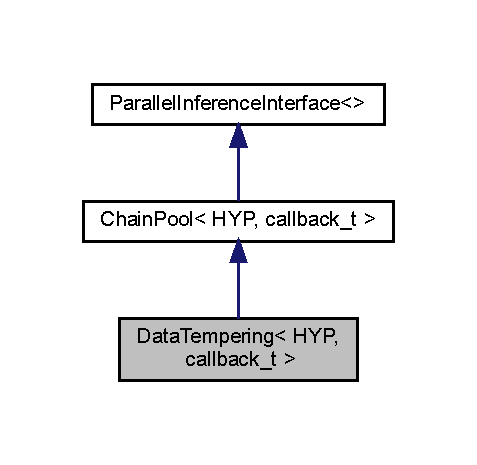
\includegraphics[width=231pt]{class_data_tempering__inherit__graph}
\end{center}
\end{figure}


Collaboration diagram for Data\+Tempering$<$ H\+YP, callback\+\_\+t $>$\+:
\nopagebreak
\begin{figure}[H]
\begin{center}
\leavevmode
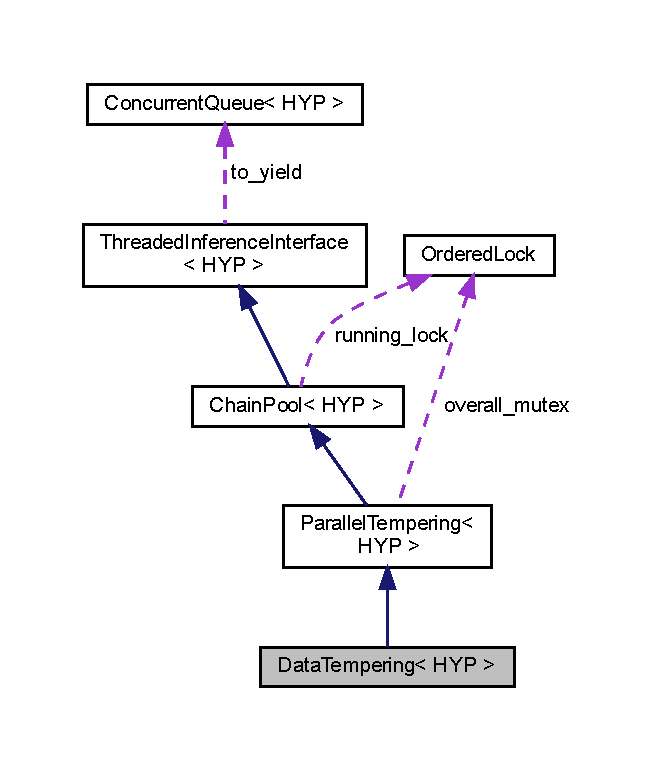
\includegraphics[width=350pt]{class_data_tempering__coll__graph}
\end{center}
\end{figure}
\subsection*{Public Member Functions}
\begin{DoxyCompactItemize}
\item 
\hyperlink{class_data_tempering_a21a8c93e110fdcebce332300bfea5ece}{Data\+Tempering} (H\+YP \&h0, std\+::vector$<$ typename H\+Y\+P\+::data\+\_\+t $>$ \&datas, std\+::vector$<$ callback\+\_\+t $>$ \&cb)
\item 
\hyperlink{class_data_tempering_a87d7969c6e9df8682d7912a5ef9cc41a}{$\sim$\+Data\+Tempering} ()
\item 
void \hyperlink{class_data_tempering_a878981d5b443b50348fcd25a03135609}{\+\_\+\+\_\+swapper\+\_\+thread} (time\+\_\+ms swap\+\_\+every)
\item 
virtual void \hyperlink{class_data_tempering_a47b07f1c97e7f65b7694efdaa088039b}{run} (\hyperlink{struct_control}{Control} ctl) override
\item 
virtual void \hyperlink{class_data_tempering_ae1fbeeddd743c7f70c2df1a4ff458f0e}{run} (\hyperlink{struct_control}{Control} ctl, time\+\_\+ms swap\+\_\+every, time\+\_\+ms adapt\+\_\+every)
\item 
void \hyperlink{class_data_tempering_a01d9f1eb405ed44f8151bd79afd2d0cc}{show\+\_\+statistics} ()
\end{DoxyCompactItemize}
\subsection*{Public Attributes}
\begin{DoxyCompactItemize}
\item 
\hyperlink{class_finite_history}{Finite\+History}$<$ bool $>$ $\ast$ \hyperlink{class_data_tempering_a1479c10bde08cccc9764267738e429eb}{swap\+\_\+history}
\item 
std\+::atomic$<$ bool $>$ \hyperlink{class_data_tempering_a03f9c6fd8faa8f88c63bbc84c388e82d}{terminate}
\end{DoxyCompactItemize}
\subsection*{Additional Inherited Members}


\subsection{Detailed Description}
\subsubsection*{template$<$typename H\+YP, typename callback\+\_\+t$>$\newline
class Data\+Tempering$<$ H\+Y\+P, callback\+\_\+t $>$}

\begin{DoxyAuthor}{Author}
piantado 
\end{DoxyAuthor}
\begin{DoxyDate}{Date}
10/06/20 
\end{DoxyDate}


\subsection{Constructor \& Destructor Documentation}
\mbox{\Hypertarget{class_data_tempering_a21a8c93e110fdcebce332300bfea5ece}\label{class_data_tempering_a21a8c93e110fdcebce332300bfea5ece}} 
\index{Data\+Tempering@{Data\+Tempering}!Data\+Tempering@{Data\+Tempering}}
\index{Data\+Tempering@{Data\+Tempering}!Data\+Tempering@{Data\+Tempering}}
\subsubsection{\texorpdfstring{Data\+Tempering()}{DataTempering()}}
{\footnotesize\ttfamily template$<$typename H\+YP , typename callback\+\_\+t $>$ \\
\hyperlink{class_data_tempering}{Data\+Tempering}$<$ H\+YP, callback\+\_\+t $>$\+::\hyperlink{class_data_tempering}{Data\+Tempering} (\begin{DoxyParamCaption}\item[{H\+YP \&}]{h0,  }\item[{std\+::vector$<$ typename H\+Y\+P\+::data\+\_\+t $>$ \&}]{datas,  }\item[{std\+::vector$<$ callback\+\_\+t $>$ \&}]{cb }\end{DoxyParamCaption})\hspace{0.3cm}{\ttfamily [inline]}}

\mbox{\Hypertarget{class_data_tempering_a87d7969c6e9df8682d7912a5ef9cc41a}\label{class_data_tempering_a87d7969c6e9df8682d7912a5ef9cc41a}} 
\index{Data\+Tempering@{Data\+Tempering}!````~Data\+Tempering@{$\sim$\+Data\+Tempering}}
\index{````~Data\+Tempering@{$\sim$\+Data\+Tempering}!Data\+Tempering@{Data\+Tempering}}
\subsubsection{\texorpdfstring{$\sim$\+Data\+Tempering()}{~DataTempering()}}
{\footnotesize\ttfamily template$<$typename H\+YP , typename callback\+\_\+t $>$ \\
\hyperlink{class_data_tempering}{Data\+Tempering}$<$ H\+YP, callback\+\_\+t $>$\+::$\sim$\hyperlink{class_data_tempering}{Data\+Tempering} (\begin{DoxyParamCaption}{ }\end{DoxyParamCaption})\hspace{0.3cm}{\ttfamily [inline]}}



\subsection{Member Function Documentation}
\mbox{\Hypertarget{class_data_tempering_a878981d5b443b50348fcd25a03135609}\label{class_data_tempering_a878981d5b443b50348fcd25a03135609}} 
\index{Data\+Tempering@{Data\+Tempering}!\+\_\+\+\_\+swapper\+\_\+thread@{\+\_\+\+\_\+swapper\+\_\+thread}}
\index{\+\_\+\+\_\+swapper\+\_\+thread@{\+\_\+\+\_\+swapper\+\_\+thread}!Data\+Tempering@{Data\+Tempering}}
\subsubsection{\texorpdfstring{\+\_\+\+\_\+swapper\+\_\+thread()}{\_\_swapper\_thread()}}
{\footnotesize\ttfamily template$<$typename H\+YP , typename callback\+\_\+t $>$ \\
void \hyperlink{class_data_tempering}{Data\+Tempering}$<$ H\+YP, callback\+\_\+t $>$\+::\+\_\+\+\_\+swapper\+\_\+thread (\begin{DoxyParamCaption}\item[{time\+\_\+ms}]{swap\+\_\+every }\end{DoxyParamCaption})\hspace{0.3cm}{\ttfamily [inline]}}

\mbox{\Hypertarget{class_data_tempering_a47b07f1c97e7f65b7694efdaa088039b}\label{class_data_tempering_a47b07f1c97e7f65b7694efdaa088039b}} 
\index{Data\+Tempering@{Data\+Tempering}!run@{run}}
\index{run@{run}!Data\+Tempering@{Data\+Tempering}}
\subsubsection{\texorpdfstring{run()}{run()}\hspace{0.1cm}{\footnotesize\ttfamily [1/2]}}
{\footnotesize\ttfamily template$<$typename H\+YP , typename callback\+\_\+t $>$ \\
virtual void \hyperlink{class_data_tempering}{Data\+Tempering}$<$ H\+YP, callback\+\_\+t $>$\+::run (\begin{DoxyParamCaption}\item[{\hyperlink{struct_control}{Control}}]{ctl }\end{DoxyParamCaption})\hspace{0.3cm}{\ttfamily [inline]}, {\ttfamily [override]}, {\ttfamily [virtual]}}

\mbox{\Hypertarget{class_data_tempering_ae1fbeeddd743c7f70c2df1a4ff458f0e}\label{class_data_tempering_ae1fbeeddd743c7f70c2df1a4ff458f0e}} 
\index{Data\+Tempering@{Data\+Tempering}!run@{run}}
\index{run@{run}!Data\+Tempering@{Data\+Tempering}}
\subsubsection{\texorpdfstring{run()}{run()}\hspace{0.1cm}{\footnotesize\ttfamily [2/2]}}
{\footnotesize\ttfamily template$<$typename H\+YP , typename callback\+\_\+t $>$ \\
virtual void \hyperlink{class_data_tempering}{Data\+Tempering}$<$ H\+YP, callback\+\_\+t $>$\+::run (\begin{DoxyParamCaption}\item[{\hyperlink{struct_control}{Control}}]{ctl,  }\item[{time\+\_\+ms}]{swap\+\_\+every,  }\item[{time\+\_\+ms}]{adapt\+\_\+every }\end{DoxyParamCaption})\hspace{0.3cm}{\ttfamily [inline]}, {\ttfamily [virtual]}}

\mbox{\Hypertarget{class_data_tempering_a01d9f1eb405ed44f8151bd79afd2d0cc}\label{class_data_tempering_a01d9f1eb405ed44f8151bd79afd2d0cc}} 
\index{Data\+Tempering@{Data\+Tempering}!show\+\_\+statistics@{show\+\_\+statistics}}
\index{show\+\_\+statistics@{show\+\_\+statistics}!Data\+Tempering@{Data\+Tempering}}
\subsubsection{\texorpdfstring{show\+\_\+statistics()}{show\_statistics()}}
{\footnotesize\ttfamily template$<$typename H\+YP , typename callback\+\_\+t $>$ \\
void \hyperlink{class_data_tempering}{Data\+Tempering}$<$ H\+YP, callback\+\_\+t $>$\+::show\+\_\+statistics (\begin{DoxyParamCaption}{ }\end{DoxyParamCaption})\hspace{0.3cm}{\ttfamily [inline]}}



\subsection{Member Data Documentation}
\mbox{\Hypertarget{class_data_tempering_a1479c10bde08cccc9764267738e429eb}\label{class_data_tempering_a1479c10bde08cccc9764267738e429eb}} 
\index{Data\+Tempering@{Data\+Tempering}!swap\+\_\+history@{swap\+\_\+history}}
\index{swap\+\_\+history@{swap\+\_\+history}!Data\+Tempering@{Data\+Tempering}}
\subsubsection{\texorpdfstring{swap\+\_\+history}{swap\_history}}
{\footnotesize\ttfamily template$<$typename H\+YP , typename callback\+\_\+t $>$ \\
\hyperlink{class_finite_history}{Finite\+History}$<$bool$>$$\ast$ \hyperlink{class_data_tempering}{Data\+Tempering}$<$ H\+YP, callback\+\_\+t $>$\+::swap\+\_\+history}

\mbox{\Hypertarget{class_data_tempering_a03f9c6fd8faa8f88c63bbc84c388e82d}\label{class_data_tempering_a03f9c6fd8faa8f88c63bbc84c388e82d}} 
\index{Data\+Tempering@{Data\+Tempering}!terminate@{terminate}}
\index{terminate@{terminate}!Data\+Tempering@{Data\+Tempering}}
\subsubsection{\texorpdfstring{terminate}{terminate}}
{\footnotesize\ttfamily template$<$typename H\+YP , typename callback\+\_\+t $>$ \\
std\+::atomic$<$bool$>$ \hyperlink{class_data_tempering}{Data\+Tempering}$<$ H\+YP, callback\+\_\+t $>$\+::terminate}



The documentation for this class was generated from the following file\+:\begin{DoxyCompactItemize}
\item 
src/\+Inference/\hyperlink{_parallel_tempering_8h}{Parallel\+Tempering.\+h}\end{DoxyCompactItemize}

\hypertarget{classdefauldatum__t}{}\section{defauldatum\+\_\+t$<$ input\+\_\+t, output\+\_\+t $>$ Class Template Reference}
\label{classdefauldatum__t}\index{defauldatum\+\_\+t$<$ input\+\_\+t, output\+\_\+t $>$@{defauldatum\+\_\+t$<$ input\+\_\+t, output\+\_\+t $>$}}


{\ttfamily \#include $<$Datum.\+h$>$}

\subsection*{Public Member Functions}
\begin{DoxyCompactItemize}
\item 
\hyperlink{classdefauldatum__t_a60dbe7a244471992011e822a274111fb}{defauldatum\+\_\+t} ()
\item 
\hyperlink{classdefauldatum__t_aec837adfff605f08b75e8157f542fb90}{defauldatum\+\_\+t} (const input\+\_\+t \&i, const output\+\_\+t \&o, double r)
\item 
\hyperlink{classdefauldatum__t_a338eb6eda0b2c7adb2b83476b57561d3}{defauldatum\+\_\+t} (const input\+\_\+t \&i, const output\+\_\+t \&o)
\item 
bool \hyperlink{classdefauldatum__t_a96eb1be1316177eb30d9bbc4a5405a9c}{operator==} (const \hyperlink{classdefauldatum__t}{defauldatum\+\_\+t} \&y) const
\end{DoxyCompactItemize}
\subsection*{Public Attributes}
\begin{DoxyCompactItemize}
\item 
input\+\_\+t \hyperlink{classdefauldatum__t_a282269cf029cd4068c94db8c8edee01e}{input}
\item 
output\+\_\+t \hyperlink{classdefauldatum__t_abe0955067e70651670dfe3031eda1efb}{output}
\item 
double \hyperlink{classdefauldatum__t_a113548381865b87bd1332d8c73e56608}{reliability}
\end{DoxyCompactItemize}


\subsection{Detailed Description}
\subsubsection*{template$<$typename input\+\_\+t, typename output\+\_\+t$>$\newline
class defauldatum\+\_\+t$<$ input\+\_\+t, output\+\_\+t $>$}

\begin{DoxyAuthor}{Author}
piantado 
\end{DoxyAuthor}
\begin{DoxyDate}{Date}
29/01/20 
\end{DoxyDate}


\subsection{Constructor \& Destructor Documentation}
\mbox{\Hypertarget{classdefauldatum__t_a60dbe7a244471992011e822a274111fb}\label{classdefauldatum__t_a60dbe7a244471992011e822a274111fb}} 
\index{defauldatum\+\_\+t@{defauldatum\+\_\+t}!defauldatum\+\_\+t@{defauldatum\+\_\+t}}
\index{defauldatum\+\_\+t@{defauldatum\+\_\+t}!defauldatum\+\_\+t@{defauldatum\+\_\+t}}
\subsubsection{\texorpdfstring{defauldatum\+\_\+t()}{defauldatum\_t()}\hspace{0.1cm}{\footnotesize\ttfamily [1/3]}}
{\footnotesize\ttfamily template$<$typename input\+\_\+t, typename output\+\_\+t$>$ \\
\hyperlink{classdefauldatum__t}{defauldatum\+\_\+t}$<$ input\+\_\+t, output\+\_\+t $>$\+::\hyperlink{classdefauldatum__t}{defauldatum\+\_\+t} (\begin{DoxyParamCaption}{ }\end{DoxyParamCaption})\hspace{0.3cm}{\ttfamily [inline]}}

\mbox{\Hypertarget{classdefauldatum__t_aec837adfff605f08b75e8157f542fb90}\label{classdefauldatum__t_aec837adfff605f08b75e8157f542fb90}} 
\index{defauldatum\+\_\+t@{defauldatum\+\_\+t}!defauldatum\+\_\+t@{defauldatum\+\_\+t}}
\index{defauldatum\+\_\+t@{defauldatum\+\_\+t}!defauldatum\+\_\+t@{defauldatum\+\_\+t}}
\subsubsection{\texorpdfstring{defauldatum\+\_\+t()}{defauldatum\_t()}\hspace{0.1cm}{\footnotesize\ttfamily [2/3]}}
{\footnotesize\ttfamily template$<$typename input\+\_\+t, typename output\+\_\+t$>$ \\
\hyperlink{classdefauldatum__t}{defauldatum\+\_\+t}$<$ input\+\_\+t, output\+\_\+t $>$\+::\hyperlink{classdefauldatum__t}{defauldatum\+\_\+t} (\begin{DoxyParamCaption}\item[{const input\+\_\+t \&}]{i,  }\item[{const output\+\_\+t \&}]{o,  }\item[{double}]{r }\end{DoxyParamCaption})\hspace{0.3cm}{\ttfamily [inline]}}

\mbox{\Hypertarget{classdefauldatum__t_a338eb6eda0b2c7adb2b83476b57561d3}\label{classdefauldatum__t_a338eb6eda0b2c7adb2b83476b57561d3}} 
\index{defauldatum\+\_\+t@{defauldatum\+\_\+t}!defauldatum\+\_\+t@{defauldatum\+\_\+t}}
\index{defauldatum\+\_\+t@{defauldatum\+\_\+t}!defauldatum\+\_\+t@{defauldatum\+\_\+t}}
\subsubsection{\texorpdfstring{defauldatum\+\_\+t()}{defauldatum\_t()}\hspace{0.1cm}{\footnotesize\ttfamily [3/3]}}
{\footnotesize\ttfamily template$<$typename input\+\_\+t, typename output\+\_\+t$>$ \\
\hyperlink{classdefauldatum__t}{defauldatum\+\_\+t}$<$ input\+\_\+t, output\+\_\+t $>$\+::\hyperlink{classdefauldatum__t}{defauldatum\+\_\+t} (\begin{DoxyParamCaption}\item[{const input\+\_\+t \&}]{i,  }\item[{const output\+\_\+t \&}]{o }\end{DoxyParamCaption})\hspace{0.3cm}{\ttfamily [inline]}}



\subsection{Member Function Documentation}
\mbox{\Hypertarget{classdefauldatum__t_a96eb1be1316177eb30d9bbc4a5405a9c}\label{classdefauldatum__t_a96eb1be1316177eb30d9bbc4a5405a9c}} 
\index{defauldatum\+\_\+t@{defauldatum\+\_\+t}!operator==@{operator==}}
\index{operator==@{operator==}!defauldatum\+\_\+t@{defauldatum\+\_\+t}}
\subsubsection{\texorpdfstring{operator==()}{operator==()}}
{\footnotesize\ttfamily template$<$typename input\+\_\+t, typename output\+\_\+t$>$ \\
bool \hyperlink{classdefauldatum__t}{defauldatum\+\_\+t}$<$ input\+\_\+t, output\+\_\+t $>$\+::operator== (\begin{DoxyParamCaption}\item[{const \hyperlink{classdefauldatum__t}{defauldatum\+\_\+t}$<$ input\+\_\+t, output\+\_\+t $>$ \&}]{y }\end{DoxyParamCaption}) const\hspace{0.3cm}{\ttfamily [inline]}}



\subsection{Member Data Documentation}
\mbox{\Hypertarget{classdefauldatum__t_a282269cf029cd4068c94db8c8edee01e}\label{classdefauldatum__t_a282269cf029cd4068c94db8c8edee01e}} 
\index{defauldatum\+\_\+t@{defauldatum\+\_\+t}!input@{input}}
\index{input@{input}!defauldatum\+\_\+t@{defauldatum\+\_\+t}}
\subsubsection{\texorpdfstring{input}{input}}
{\footnotesize\ttfamily template$<$typename input\+\_\+t, typename output\+\_\+t$>$ \\
input\+\_\+t \hyperlink{classdefauldatum__t}{defauldatum\+\_\+t}$<$ input\+\_\+t, output\+\_\+t $>$\+::input}

\mbox{\Hypertarget{classdefauldatum__t_abe0955067e70651670dfe3031eda1efb}\label{classdefauldatum__t_abe0955067e70651670dfe3031eda1efb}} 
\index{defauldatum\+\_\+t@{defauldatum\+\_\+t}!output@{output}}
\index{output@{output}!defauldatum\+\_\+t@{defauldatum\+\_\+t}}
\subsubsection{\texorpdfstring{output}{output}}
{\footnotesize\ttfamily template$<$typename input\+\_\+t, typename output\+\_\+t$>$ \\
output\+\_\+t \hyperlink{classdefauldatum__t}{defauldatum\+\_\+t}$<$ input\+\_\+t, output\+\_\+t $>$\+::output}

\mbox{\Hypertarget{classdefauldatum__t_a113548381865b87bd1332d8c73e56608}\label{classdefauldatum__t_a113548381865b87bd1332d8c73e56608}} 
\index{defauldatum\+\_\+t@{defauldatum\+\_\+t}!reliability@{reliability}}
\index{reliability@{reliability}!defauldatum\+\_\+t@{defauldatum\+\_\+t}}
\subsubsection{\texorpdfstring{reliability}{reliability}}
{\footnotesize\ttfamily template$<$typename input\+\_\+t, typename output\+\_\+t$>$ \\
double \hyperlink{classdefauldatum__t}{defauldatum\+\_\+t}$<$ input\+\_\+t, output\+\_\+t $>$\+::reliability}



The documentation for this class was generated from the following file\+:\begin{DoxyCompactItemize}
\item 
src/\+Hypotheses/\hyperlink{_datum_8h}{Datum.\+h}\end{DoxyCompactItemize}

\hypertarget{class_discrete_distribution}{}\doxysection{Discrete\+Distribution$<$ T $>$ Class Template Reference}
\label{class_discrete_distribution}\index{DiscreteDistribution$<$ T $>$@{DiscreteDistribution$<$ T $>$}}


{\ttfamily \#include $<$Discrete\+Distribution.\+h$>$}

\doxysubsection*{Public Member Functions}
\begin{DoxyCompactItemize}
\item 
\mbox{\hyperlink{class_discrete_distribution_a8ffb7c55f85cf42af7aec6deb97ec4ab}{Discrete\+Distribution}} ()
\item 
virtual T \mbox{\hyperlink{class_discrete_distribution_a7cf660223fe0f86b61e3b33268204c06}{argmax}} () const
\item 
void \mbox{\hyperlink{class_discrete_distribution_a6ec6f590a3659c8bef32aaab77a8052e}{print}} (std\+::ostream \&out, unsigned long nprint=0) const
\item 
void \mbox{\hyperlink{class_discrete_distribution_a58bc689015e6b594ed1a53130758ba6f}{print}} (unsigned long nprint=0) const
\item 
std\+::string \mbox{\hyperlink{class_discrete_distribution_a87d866919f4698e488aee9ce4bc42ed5}{string}} (unsigned long nprint=0) const
\item 
void \mbox{\hyperlink{class_discrete_distribution_a6c41c7f4726019bc213d37d4e3cdea27}{addmass}} (T x, double v)
\item 
const std\+::map$<$ T, double $>$ \& \mbox{\hyperlink{class_discrete_distribution_a995377a760a6fe0d44077892053acdbb}{values}} () const
\item 
void \mbox{\hyperlink{class_discrete_distribution_a5c93983e2375a2353b10b82ebb11f751}{operator$<$$<$}} (const \mbox{\hyperlink{class_discrete_distribution}{Discrete\+Distribution}}$<$ T $>$ \&x)
\item 
double \mbox{\hyperlink{class_discrete_distribution_ad634a339172a69c006fded1beb423bb7}{Z}} () const
\item 
double \mbox{\hyperlink{class_discrete_distribution_a185ef689b1e133b962fff5bcf1443ba1}{lp}} (const T \&x)
\item 
std\+::vector$<$ T $>$ \mbox{\hyperlink{class_discrete_distribution_adee72a8e4c93aa03d841c0c73d6b5498}{best}} (size\+\_\+t N) const
\item 
std\+::vector$<$ std\+::pair$<$ T, double $>$ $>$ \mbox{\hyperlink{class_discrete_distribution_a94488cfd094f6cde47f15a1f4c7cdbb9}{sorted}} (bool decreasing=false) const
\item 
size\+\_\+t \mbox{\hyperlink{class_discrete_distribution_afd3fd83dc776f5616e826de18093328b}{count}} (T x) const
\item 
size\+\_\+t \mbox{\hyperlink{class_discrete_distribution_ad74207d32c2ed6c5c26b3f991f4fedba}{size}} () const
\item 
double \mbox{\hyperlink{class_discrete_distribution_a374bcf1a5b302e6ac618afe9d78e265f}{operator\mbox{[}$\,$\mbox{]}}} (const T x)
\item 
double \mbox{\hyperlink{class_discrete_distribution_acb11f1cfbf4ef039c538f06cde8249fd}{at}} (T x) const
\end{DoxyCompactItemize}
\doxysubsection*{Public Attributes}
\begin{DoxyCompactItemize}
\item 
std\+::map$<$ T, double $>$ \mbox{\hyperlink{class_discrete_distribution_a72a09b5b79a5bf0c55f780b9a81271fb}{m}}
\end{DoxyCompactItemize}


\doxysubsection{Detailed Description}
\subsubsection*{template$<$typename T$>$\newline
class Discrete\+Distribution$<$ T $>$}

\begin{DoxyAuthor}{Author}
steven piantadosi 
\end{DoxyAuthor}
\begin{DoxyDate}{Date}
03/02/20 
\end{DoxyDate}


\doxysubsection{Constructor \& Destructor Documentation}
\mbox{\Hypertarget{class_discrete_distribution_a8ffb7c55f85cf42af7aec6deb97ec4ab}\label{class_discrete_distribution_a8ffb7c55f85cf42af7aec6deb97ec4ab}} 
\index{DiscreteDistribution$<$ T $>$@{DiscreteDistribution$<$ T $>$}!DiscreteDistribution@{DiscreteDistribution}}
\index{DiscreteDistribution@{DiscreteDistribution}!DiscreteDistribution$<$ T $>$@{DiscreteDistribution$<$ T $>$}}
\doxysubsubsection{\texorpdfstring{DiscreteDistribution()}{DiscreteDistribution()}}
{\footnotesize\ttfamily template$<$typename T $>$ \\
\mbox{\hyperlink{class_discrete_distribution}{Discrete\+Distribution}}$<$ T $>$\+::\mbox{\hyperlink{class_discrete_distribution}{Discrete\+Distribution}} (\begin{DoxyParamCaption}{ }\end{DoxyParamCaption})\hspace{0.3cm}{\ttfamily [inline]}}



\doxysubsection{Member Function Documentation}
\mbox{\Hypertarget{class_discrete_distribution_a6c41c7f4726019bc213d37d4e3cdea27}\label{class_discrete_distribution_a6c41c7f4726019bc213d37d4e3cdea27}} 
\index{DiscreteDistribution$<$ T $>$@{DiscreteDistribution$<$ T $>$}!addmass@{addmass}}
\index{addmass@{addmass}!DiscreteDistribution$<$ T $>$@{DiscreteDistribution$<$ T $>$}}
\doxysubsubsection{\texorpdfstring{addmass()}{addmass()}}
{\footnotesize\ttfamily template$<$typename T $>$ \\
void \mbox{\hyperlink{class_discrete_distribution}{Discrete\+Distribution}}$<$ T $>$\+::addmass (\begin{DoxyParamCaption}\item[{T}]{x,  }\item[{double}]{v }\end{DoxyParamCaption})\hspace{0.3cm}{\ttfamily [inline]}}

Add log probability v to type x 
\begin{DoxyParams}{Parameters}
{\em x} & \\
\hline
{\em v} & \\
\hline
\end{DoxyParams}
\mbox{\Hypertarget{class_discrete_distribution_a7cf660223fe0f86b61e3b33268204c06}\label{class_discrete_distribution_a7cf660223fe0f86b61e3b33268204c06}} 
\index{DiscreteDistribution$<$ T $>$@{DiscreteDistribution$<$ T $>$}!argmax@{argmax}}
\index{argmax@{argmax}!DiscreteDistribution$<$ T $>$@{DiscreteDistribution$<$ T $>$}}
\doxysubsubsection{\texorpdfstring{argmax()}{argmax()}}
{\footnotesize\ttfamily template$<$typename T $>$ \\
virtual T \mbox{\hyperlink{class_discrete_distribution}{Discrete\+Distribution}}$<$ T $>$\+::argmax (\begin{DoxyParamCaption}{ }\end{DoxyParamCaption}) const\hspace{0.3cm}{\ttfamily [inline]}, {\ttfamily [virtual]}}

\mbox{\Hypertarget{class_discrete_distribution_acb11f1cfbf4ef039c538f06cde8249fd}\label{class_discrete_distribution_acb11f1cfbf4ef039c538f06cde8249fd}} 
\index{DiscreteDistribution$<$ T $>$@{DiscreteDistribution$<$ T $>$}!at@{at}}
\index{at@{at}!DiscreteDistribution$<$ T $>$@{DiscreteDistribution$<$ T $>$}}
\doxysubsubsection{\texorpdfstring{at()}{at()}}
{\footnotesize\ttfamily template$<$typename T $>$ \\
double \mbox{\hyperlink{class_discrete_distribution}{Discrete\+Distribution}}$<$ T $>$\+::at (\begin{DoxyParamCaption}\item[{T}]{x }\end{DoxyParamCaption}) const\hspace{0.3cm}{\ttfamily [inline]}}

\mbox{\Hypertarget{class_discrete_distribution_adee72a8e4c93aa03d841c0c73d6b5498}\label{class_discrete_distribution_adee72a8e4c93aa03d841c0c73d6b5498}} 
\index{DiscreteDistribution$<$ T $>$@{DiscreteDistribution$<$ T $>$}!best@{best}}
\index{best@{best}!DiscreteDistribution$<$ T $>$@{DiscreteDistribution$<$ T $>$}}
\doxysubsubsection{\texorpdfstring{best()}{best()}}
{\footnotesize\ttfamily template$<$typename T $>$ \\
std\+::vector$<$T$>$ \mbox{\hyperlink{class_discrete_distribution}{Discrete\+Distribution}}$<$ T $>$\+::best (\begin{DoxyParamCaption}\item[{size\+\_\+t}]{N }\end{DoxyParamCaption}) const\hspace{0.3cm}{\ttfamily [inline]}}

Get the N best from this distribution 
\begin{DoxyParams}{Parameters}
{\em N} & \\
\hline
\end{DoxyParams}
\begin{DoxyReturn}{Returns}

\end{DoxyReturn}
\mbox{\Hypertarget{class_discrete_distribution_afd3fd83dc776f5616e826de18093328b}\label{class_discrete_distribution_afd3fd83dc776f5616e826de18093328b}} 
\index{DiscreteDistribution$<$ T $>$@{DiscreteDistribution$<$ T $>$}!count@{count}}
\index{count@{count}!DiscreteDistribution$<$ T $>$@{DiscreteDistribution$<$ T $>$}}
\doxysubsubsection{\texorpdfstring{count()}{count()}}
{\footnotesize\ttfamily template$<$typename T $>$ \\
size\+\_\+t \mbox{\hyperlink{class_discrete_distribution}{Discrete\+Distribution}}$<$ T $>$\+::count (\begin{DoxyParamCaption}\item[{T}]{x }\end{DoxyParamCaption}) const\hspace{0.3cm}{\ttfamily [inline]}}

\mbox{\Hypertarget{class_discrete_distribution_a185ef689b1e133b962fff5bcf1443ba1}\label{class_discrete_distribution_a185ef689b1e133b962fff5bcf1443ba1}} 
\index{DiscreteDistribution$<$ T $>$@{DiscreteDistribution$<$ T $>$}!lp@{lp}}
\index{lp@{lp}!DiscreteDistribution$<$ T $>$@{DiscreteDistribution$<$ T $>$}}
\doxysubsubsection{\texorpdfstring{lp()}{lp()}}
{\footnotesize\ttfamily template$<$typename T $>$ \\
double \mbox{\hyperlink{class_discrete_distribution}{Discrete\+Distribution}}$<$ T $>$\+::lp (\begin{DoxyParamCaption}\item[{const T \&}]{x }\end{DoxyParamCaption})\hspace{0.3cm}{\ttfamily [inline]}}

Retun the log probability of x, including the normalizing term (N\+O\+TE\+: This makes this O(\+N) to compute theo normalizer. So this is bad to use if you have to iterate over the set -- you shoul call \mbox{\hyperlink{class_discrete_distribution_ad634a339172a69c006fded1beb423bb7}{Z()}} separately then 
\begin{DoxyParams}{Parameters}
{\em N} & \\
\hline
\end{DoxyParams}
\begin{DoxyReturn}{Returns}

\end{DoxyReturn}
\mbox{\Hypertarget{class_discrete_distribution_a5c93983e2375a2353b10b82ebb11f751}\label{class_discrete_distribution_a5c93983e2375a2353b10b82ebb11f751}} 
\index{DiscreteDistribution$<$ T $>$@{DiscreteDistribution$<$ T $>$}!operator$<$$<$@{operator$<$$<$}}
\index{operator$<$$<$@{operator$<$$<$}!DiscreteDistribution$<$ T $>$@{DiscreteDistribution$<$ T $>$}}
\doxysubsubsection{\texorpdfstring{operator$<$$<$()}{operator<<()}}
{\footnotesize\ttfamily template$<$typename T $>$ \\
void \mbox{\hyperlink{class_discrete_distribution}{Discrete\+Distribution}}$<$ T $>$\+::operator$<$$<$ (\begin{DoxyParamCaption}\item[{const \mbox{\hyperlink{class_discrete_distribution}{Discrete\+Distribution}}$<$ T $>$ \&}]{x }\end{DoxyParamCaption})\hspace{0.3cm}{\ttfamily [inline]}}

\mbox{\Hypertarget{class_discrete_distribution_a374bcf1a5b302e6ac618afe9d78e265f}\label{class_discrete_distribution_a374bcf1a5b302e6ac618afe9d78e265f}} 
\index{DiscreteDistribution$<$ T $>$@{DiscreteDistribution$<$ T $>$}!operator\mbox{[}\mbox{]}@{operator[]}}
\index{operator\mbox{[}\mbox{]}@{operator[]}!DiscreteDistribution$<$ T $>$@{DiscreteDistribution$<$ T $>$}}
\doxysubsubsection{\texorpdfstring{operator[]()}{operator[]()}}
{\footnotesize\ttfamily template$<$typename T $>$ \\
double \mbox{\hyperlink{class_discrete_distribution}{Discrete\+Distribution}}$<$ T $>$\+::operator\mbox{[}$\,$\mbox{]} (\begin{DoxyParamCaption}\item[{const T}]{x }\end{DoxyParamCaption})\hspace{0.3cm}{\ttfamily [inline]}}

\mbox{\Hypertarget{class_discrete_distribution_a6ec6f590a3659c8bef32aaab77a8052e}\label{class_discrete_distribution_a6ec6f590a3659c8bef32aaab77a8052e}} 
\index{DiscreteDistribution$<$ T $>$@{DiscreteDistribution$<$ T $>$}!print@{print}}
\index{print@{print}!DiscreteDistribution$<$ T $>$@{DiscreteDistribution$<$ T $>$}}
\doxysubsubsection{\texorpdfstring{print()}{print()}\hspace{0.1cm}{\footnotesize\ttfamily [1/2]}}
{\footnotesize\ttfamily template$<$typename T $>$ \\
void \mbox{\hyperlink{class_discrete_distribution}{Discrete\+Distribution}}$<$ T $>$\+::print (\begin{DoxyParamCaption}\item[{std\+::ostream \&}]{out,  }\item[{unsigned long}]{nprint = {\ttfamily 0} }\end{DoxyParamCaption}) const\hspace{0.3cm}{\ttfamily [inline]}}

\mbox{\Hypertarget{class_discrete_distribution_a58bc689015e6b594ed1a53130758ba6f}\label{class_discrete_distribution_a58bc689015e6b594ed1a53130758ba6f}} 
\index{DiscreteDistribution$<$ T $>$@{DiscreteDistribution$<$ T $>$}!print@{print}}
\index{print@{print}!DiscreteDistribution$<$ T $>$@{DiscreteDistribution$<$ T $>$}}
\doxysubsubsection{\texorpdfstring{print()}{print()}\hspace{0.1cm}{\footnotesize\ttfamily [2/2]}}
{\footnotesize\ttfamily template$<$typename T $>$ \\
void \mbox{\hyperlink{class_discrete_distribution}{Discrete\+Distribution}}$<$ T $>$\+::print (\begin{DoxyParamCaption}\item[{unsigned long}]{nprint = {\ttfamily 0} }\end{DoxyParamCaption}) const\hspace{0.3cm}{\ttfamily [inline]}}

\mbox{\Hypertarget{class_discrete_distribution_ad74207d32c2ed6c5c26b3f991f4fedba}\label{class_discrete_distribution_ad74207d32c2ed6c5c26b3f991f4fedba}} 
\index{DiscreteDistribution$<$ T $>$@{DiscreteDistribution$<$ T $>$}!size@{size}}
\index{size@{size}!DiscreteDistribution$<$ T $>$@{DiscreteDistribution$<$ T $>$}}
\doxysubsubsection{\texorpdfstring{size()}{size()}}
{\footnotesize\ttfamily template$<$typename T $>$ \\
size\+\_\+t \mbox{\hyperlink{class_discrete_distribution}{Discrete\+Distribution}}$<$ T $>$\+::size (\begin{DoxyParamCaption}{ }\end{DoxyParamCaption}) const\hspace{0.3cm}{\ttfamily [inline]}}

\mbox{\Hypertarget{class_discrete_distribution_a94488cfd094f6cde47f15a1f4c7cdbb9}\label{class_discrete_distribution_a94488cfd094f6cde47f15a1f4c7cdbb9}} 
\index{DiscreteDistribution$<$ T $>$@{DiscreteDistribution$<$ T $>$}!sorted@{sorted}}
\index{sorted@{sorted}!DiscreteDistribution$<$ T $>$@{DiscreteDistribution$<$ T $>$}}
\doxysubsubsection{\texorpdfstring{sorted()}{sorted()}}
{\footnotesize\ttfamily template$<$typename T $>$ \\
std\+::vector$<$std\+::pair$<$T,double$>$ $>$ \mbox{\hyperlink{class_discrete_distribution}{Discrete\+Distribution}}$<$ T $>$\+::sorted (\begin{DoxyParamCaption}\item[{bool}]{decreasing = {\ttfamily false} }\end{DoxyParamCaption}) const\hspace{0.3cm}{\ttfamily [inline]}}

Get this distribution as a sorted vector of pairs 
\begin{DoxyParams}{Parameters}
{\em decreasing} & \\
\hline
\end{DoxyParams}
\mbox{\Hypertarget{class_discrete_distribution_a87d866919f4698e488aee9ce4bc42ed5}\label{class_discrete_distribution_a87d866919f4698e488aee9ce4bc42ed5}} 
\index{DiscreteDistribution$<$ T $>$@{DiscreteDistribution$<$ T $>$}!string@{string}}
\index{string@{string}!DiscreteDistribution$<$ T $>$@{DiscreteDistribution$<$ T $>$}}
\doxysubsubsection{\texorpdfstring{string()}{string()}}
{\footnotesize\ttfamily template$<$typename T $>$ \\
std\+::string \mbox{\hyperlink{class_discrete_distribution}{Discrete\+Distribution}}$<$ T $>$\+::string (\begin{DoxyParamCaption}\item[{unsigned long}]{nprint = {\ttfamily 0} }\end{DoxyParamCaption}) const\hspace{0.3cm}{\ttfamily [inline]}}

Convert this distribution into a string, printing at most nprint 
\begin{DoxyParams}{Parameters}
{\em nprint} & \\
\hline
\end{DoxyParams}
\begin{DoxyReturn}{Returns}

\end{DoxyReturn}
\mbox{\Hypertarget{class_discrete_distribution_a995377a760a6fe0d44077892053acdbb}\label{class_discrete_distribution_a995377a760a6fe0d44077892053acdbb}} 
\index{DiscreteDistribution$<$ T $>$@{DiscreteDistribution$<$ T $>$}!values@{values}}
\index{values@{values}!DiscreteDistribution$<$ T $>$@{DiscreteDistribution$<$ T $>$}}
\doxysubsubsection{\texorpdfstring{values()}{values()}}
{\footnotesize\ttfamily template$<$typename T $>$ \\
const std\+::map$<$T,double$>$\& \mbox{\hyperlink{class_discrete_distribution}{Discrete\+Distribution}}$<$ T $>$\+::values (\begin{DoxyParamCaption}{ }\end{DoxyParamCaption}) const\hspace{0.3cm}{\ttfamily [inline]}}

Get all of the values in this distribution \begin{DoxyReturn}{Returns}

\end{DoxyReturn}
\mbox{\Hypertarget{class_discrete_distribution_ad634a339172a69c006fded1beb423bb7}\label{class_discrete_distribution_ad634a339172a69c006fded1beb423bb7}} 
\index{DiscreteDistribution$<$ T $>$@{DiscreteDistribution$<$ T $>$}!Z@{Z}}
\index{Z@{Z}!DiscreteDistribution$<$ T $>$@{DiscreteDistribution$<$ T $>$}}
\doxysubsubsection{\texorpdfstring{Z()}{Z()}}
{\footnotesize\ttfamily template$<$typename T $>$ \\
double \mbox{\hyperlink{class_discrete_distribution}{Discrete\+Distribution}}$<$ T $>$\+::Z (\begin{DoxyParamCaption}{ }\end{DoxyParamCaption}) const\hspace{0.3cm}{\ttfamily [inline]}}



\doxysubsection{Member Data Documentation}
\mbox{\Hypertarget{class_discrete_distribution_a72a09b5b79a5bf0c55f780b9a81271fb}\label{class_discrete_distribution_a72a09b5b79a5bf0c55f780b9a81271fb}} 
\index{DiscreteDistribution$<$ T $>$@{DiscreteDistribution$<$ T $>$}!m@{m}}
\index{m@{m}!DiscreteDistribution$<$ T $>$@{DiscreteDistribution$<$ T $>$}}
\doxysubsubsection{\texorpdfstring{m}{m}}
{\footnotesize\ttfamily template$<$typename T $>$ \\
std\+::map$<$T,double$>$ \mbox{\hyperlink{class_discrete_distribution}{Discrete\+Distribution}}$<$ T $>$\+::m}



The documentation for this class was generated from the following file\+:\begin{DoxyCompactItemize}
\item 
src/\+Containers/\mbox{\hyperlink{_discrete_distribution_8h}{Discrete\+Distribution.\+h}}\end{DoxyCompactItemize}

\hypertarget{class_enumeration_inference}{}\section{Enumeration\+Inference$<$ H\+YP, Grammar\+\_\+t, callback\+\_\+t, Enumerator $>$ Class Template Reference}
\label{class_enumeration_inference}\index{Enumeration\+Inference$<$ H\+Y\+P, Grammar\+\_\+t, callback\+\_\+t, Enumerator $>$@{Enumeration\+Inference$<$ H\+Y\+P, Grammar\+\_\+t, callback\+\_\+t, Enumerator $>$}}


{\ttfamily \#include $<$Enumeration\+Inference.\+h$>$}



Inheritance diagram for Enumeration\+Inference$<$ H\+YP, Grammar\+\_\+t, callback\+\_\+t, Enumerator $>$\+:
\nopagebreak
\begin{figure}[H]
\begin{center}
\leavevmode
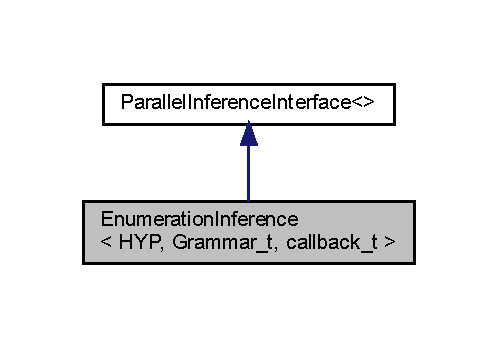
\includegraphics[width=223pt]{class_enumeration_inference__inherit__graph}
\end{center}
\end{figure}


Collaboration diagram for Enumeration\+Inference$<$ H\+YP, Grammar\+\_\+t, callback\+\_\+t, Enumerator $>$\+:
\nopagebreak
\begin{figure}[H]
\begin{center}
\leavevmode
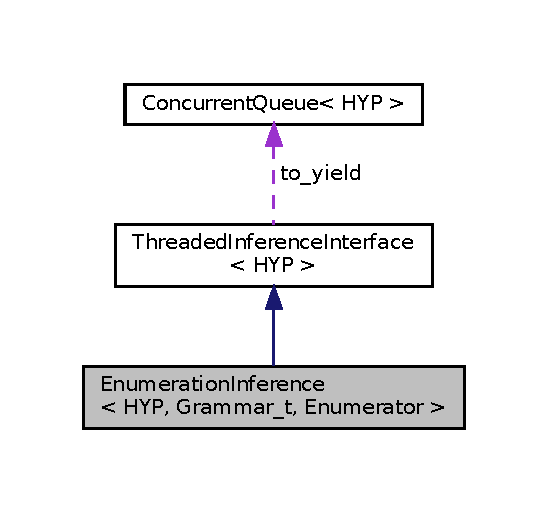
\includegraphics[width=223pt]{class_enumeration_inference__coll__graph}
\end{center}
\end{figure}
\subsection*{Public Member Functions}
\begin{DoxyCompactItemize}
\item 
\hyperlink{class_enumeration_inference_a0726b90614680808bb5ac87ca440a683}{Enumeration\+Inference} (Grammar\+\_\+t $\ast$g, typename H\+Y\+P\+::data\+\_\+t $\ast$d, callback\+\_\+t \&cb)
\item 
void \hyperlink{class_enumeration_inference_a128e8af05312e3a4a537e90ceb45c5ba}{run\+\_\+thread} (\hyperlink{struct_control}{Control} ctl) override
\end{DoxyCompactItemize}
\subsection*{Public Attributes}
\begin{DoxyCompactItemize}
\item 
Grammar\+\_\+t $\ast$ \hyperlink{class_enumeration_inference_aa39598587ac2d15550f8f9c6ca0c7089}{grammar}
\item 
H\+Y\+P\+::data\+\_\+t $\ast$ \hyperlink{class_enumeration_inference_a04537935bdd05d4320a51b15ddbca015}{data}
\item 
callback\+\_\+t $\ast$ \hyperlink{class_enumeration_inference_a25d87b73385c434bdc34192b3408c0d0}{callback}
\end{DoxyCompactItemize}


\subsection{Detailed Description}
\subsubsection*{template$<$typename H\+YP, typename Grammar\+\_\+t, typename callback\+\_\+t, typename Enumerator$>$\newline
class Enumeration\+Inference$<$ H\+Y\+P, Grammar\+\_\+t, callback\+\_\+t, Enumerator $>$}

\begin{DoxyAuthor}{Author}
piantado 
\end{DoxyAuthor}
\begin{DoxyDate}{Date}
09/06/20 
\end{DoxyDate}


\subsection{Constructor \& Destructor Documentation}
\mbox{\Hypertarget{class_enumeration_inference_a0726b90614680808bb5ac87ca440a683}\label{class_enumeration_inference_a0726b90614680808bb5ac87ca440a683}} 
\index{Enumeration\+Inference@{Enumeration\+Inference}!Enumeration\+Inference@{Enumeration\+Inference}}
\index{Enumeration\+Inference@{Enumeration\+Inference}!Enumeration\+Inference@{Enumeration\+Inference}}
\subsubsection{\texorpdfstring{Enumeration\+Inference()}{EnumerationInference()}}
{\footnotesize\ttfamily template$<$typename H\+YP , typename Grammar\+\_\+t , typename callback\+\_\+t , typename Enumerator $>$ \\
\hyperlink{class_enumeration_inference}{Enumeration\+Inference}$<$ H\+YP, Grammar\+\_\+t, callback\+\_\+t, Enumerator $>$\+::\hyperlink{class_enumeration_inference}{Enumeration\+Inference} (\begin{DoxyParamCaption}\item[{Grammar\+\_\+t $\ast$}]{g,  }\item[{typename H\+Y\+P\+::data\+\_\+t $\ast$}]{d,  }\item[{callback\+\_\+t \&}]{cb }\end{DoxyParamCaption})\hspace{0.3cm}{\ttfamily [inline]}}



\subsection{Member Function Documentation}
\mbox{\Hypertarget{class_enumeration_inference_a128e8af05312e3a4a537e90ceb45c5ba}\label{class_enumeration_inference_a128e8af05312e3a4a537e90ceb45c5ba}} 
\index{Enumeration\+Inference@{Enumeration\+Inference}!run\+\_\+thread@{run\+\_\+thread}}
\index{run\+\_\+thread@{run\+\_\+thread}!Enumeration\+Inference@{Enumeration\+Inference}}
\subsubsection{\texorpdfstring{run\+\_\+thread()}{run\_thread()}}
{\footnotesize\ttfamily template$<$typename H\+YP , typename Grammar\+\_\+t , typename callback\+\_\+t , typename Enumerator $>$ \\
void \hyperlink{class_enumeration_inference}{Enumeration\+Inference}$<$ H\+YP, Grammar\+\_\+t, callback\+\_\+t, Enumerator $>$\+::run\+\_\+thread (\begin{DoxyParamCaption}\item[{\hyperlink{struct_control}{Control}}]{ctl }\end{DoxyParamCaption})\hspace{0.3cm}{\ttfamily [inline]}, {\ttfamily [override]}}



\subsection{Member Data Documentation}
\mbox{\Hypertarget{class_enumeration_inference_a25d87b73385c434bdc34192b3408c0d0}\label{class_enumeration_inference_a25d87b73385c434bdc34192b3408c0d0}} 
\index{Enumeration\+Inference@{Enumeration\+Inference}!callback@{callback}}
\index{callback@{callback}!Enumeration\+Inference@{Enumeration\+Inference}}
\subsubsection{\texorpdfstring{callback}{callback}}
{\footnotesize\ttfamily template$<$typename H\+YP , typename Grammar\+\_\+t , typename callback\+\_\+t , typename Enumerator $>$ \\
callback\+\_\+t$\ast$ \hyperlink{class_enumeration_inference}{Enumeration\+Inference}$<$ H\+YP, Grammar\+\_\+t, callback\+\_\+t, Enumerator $>$\+::callback}

\mbox{\Hypertarget{class_enumeration_inference_a04537935bdd05d4320a51b15ddbca015}\label{class_enumeration_inference_a04537935bdd05d4320a51b15ddbca015}} 
\index{Enumeration\+Inference@{Enumeration\+Inference}!data@{data}}
\index{data@{data}!Enumeration\+Inference@{Enumeration\+Inference}}
\subsubsection{\texorpdfstring{data}{data}}
{\footnotesize\ttfamily template$<$typename H\+YP , typename Grammar\+\_\+t , typename callback\+\_\+t , typename Enumerator $>$ \\
H\+Y\+P\+::data\+\_\+t$\ast$ \hyperlink{class_enumeration_inference}{Enumeration\+Inference}$<$ H\+YP, Grammar\+\_\+t, callback\+\_\+t, Enumerator $>$\+::data}

\mbox{\Hypertarget{class_enumeration_inference_aa39598587ac2d15550f8f9c6ca0c7089}\label{class_enumeration_inference_aa39598587ac2d15550f8f9c6ca0c7089}} 
\index{Enumeration\+Inference@{Enumeration\+Inference}!grammar@{grammar}}
\index{grammar@{grammar}!Enumeration\+Inference@{Enumeration\+Inference}}
\subsubsection{\texorpdfstring{grammar}{grammar}}
{\footnotesize\ttfamily template$<$typename H\+YP , typename Grammar\+\_\+t , typename callback\+\_\+t , typename Enumerator $>$ \\
Grammar\+\_\+t$\ast$ \hyperlink{class_enumeration_inference}{Enumeration\+Inference}$<$ H\+YP, Grammar\+\_\+t, callback\+\_\+t, Enumerator $>$\+::grammar}



The documentation for this class was generated from the following file\+:\begin{DoxyCompactItemize}
\item 
src/\+Inference/\hyperlink{_inference_2_enumeration_inference_8h}{Enumeration\+Inference.\+h}\end{DoxyCompactItemize}

\hypertarget{class_finite_history}{}\section{Finite\+History$<$ T $>$ Class Template Reference}
\label{class_finite_history}\index{Finite\+History$<$ T $>$@{Finite\+History$<$ T $>$}}


{\ttfamily \#include $<$Finite\+History.\+h$>$}

\subsection*{Public Member Functions}
\begin{DoxyCompactItemize}
\item 
\hyperlink{class_finite_history_a9300fde1231d7307a97349caa4745b1a}{Finite\+History} (size\+\_\+t n)
\item 
\hyperlink{class_finite_history_a845a1fd7ec4b850c2ee6ec2003c6bd3e}{Finite\+History} ()
\item 
\hyperlink{class_finite_history_a601fa98e570953c9d0e9a562a24b92c1}{Finite\+History} (const \hyperlink{class_finite_history}{Finite\+History} \&fh)
\item 
\hyperlink{class_finite_history_ade3eff280584fefaf796c70912781825}{Finite\+History} (\hyperlink{class_finite_history}{Finite\+History} \&\&fh)
\item 
void \hyperlink{class_finite_history_afdc27d66ff1c1c386185f29eff5c474c}{operator=} (const \hyperlink{class_finite_history}{Finite\+History} \&fh)
\item 
void \hyperlink{class_finite_history_a1c3695b639cd2ec5cda375c4450b3cc8}{operator=} (\hyperlink{class_finite_history}{Finite\+History} \&\&fh)
\item 
void \hyperlink{class_finite_history_ae7e85a666c78b8d21276758ac1c2f22f}{add} (T x)
\begin{DoxyCompactList}\small\item\em Add x to this history. \end{DoxyCompactList}\item 
void \hyperlink{class_finite_history_aec85dc2f48062985164e4033223d9312}{operator$<$$<$} (T x)
\begin{DoxyCompactList}\small\item\em Convenient adding. \end{DoxyCompactList}\item 
double \hyperlink{class_finite_history_a1184d6b1d30c2d4d86846a643dbee18a}{mean} ()
\begin{DoxyCompactList}\small\item\em Compute the average. \end{DoxyCompactList}\end{DoxyCompactItemize}
\subsection*{Public Attributes}
\begin{DoxyCompactItemize}
\item 
std\+::vector$<$ T $>$ \hyperlink{class_finite_history_ae11bec06f0aca5c036d3e44dfe998cbe}{history}
\item 
std\+::atomic$<$ size\+\_\+t $>$ \hyperlink{class_finite_history_aa744ad1f9f0ef54fbd575eef672adc08}{history\+\_\+size}
\item 
std\+::atomic$<$ size\+\_\+t $>$ \hyperlink{class_finite_history_a1730270169bb022306e9a40e871aec35}{history\+\_\+index}
\item 
std\+::atomic$<$ unsigned long $>$ \hyperlink{class_finite_history_a5967a95efc3ef8aa4391942da511eab7}{N}
\item 
std\+::mutex \hyperlink{class_finite_history_a677c5c1c7115d5c8c8381aa4332025c6}{mutex}
\end{DoxyCompactItemize}


\subsection{Detailed Description}
\subsubsection*{template$<$typename T$>$\newline
class Finite\+History$<$ T $>$}

\begin{DoxyAuthor}{Author}
steven piantadosi 
\end{DoxyAuthor}
\begin{DoxyDate}{Date}
03/02/20 
\end{DoxyDate}


\subsection{Constructor \& Destructor Documentation}
\mbox{\Hypertarget{class_finite_history_a9300fde1231d7307a97349caa4745b1a}\label{class_finite_history_a9300fde1231d7307a97349caa4745b1a}} 
\index{Finite\+History@{Finite\+History}!Finite\+History@{Finite\+History}}
\index{Finite\+History@{Finite\+History}!Finite\+History@{Finite\+History}}
\subsubsection{\texorpdfstring{Finite\+History()}{FiniteHistory()}\hspace{0.1cm}{\footnotesize\ttfamily [1/4]}}
{\footnotesize\ttfamily template$<$typename T$>$ \\
\hyperlink{class_finite_history}{Finite\+History}$<$ T $>$\+::\hyperlink{class_finite_history}{Finite\+History} (\begin{DoxyParamCaption}\item[{size\+\_\+t}]{n }\end{DoxyParamCaption})\hspace{0.3cm}{\ttfamily [inline]}}

\mbox{\Hypertarget{class_finite_history_a845a1fd7ec4b850c2ee6ec2003c6bd3e}\label{class_finite_history_a845a1fd7ec4b850c2ee6ec2003c6bd3e}} 
\index{Finite\+History@{Finite\+History}!Finite\+History@{Finite\+History}}
\index{Finite\+History@{Finite\+History}!Finite\+History@{Finite\+History}}
\subsubsection{\texorpdfstring{Finite\+History()}{FiniteHistory()}\hspace{0.1cm}{\footnotesize\ttfamily [2/4]}}
{\footnotesize\ttfamily template$<$typename T$>$ \\
\hyperlink{class_finite_history}{Finite\+History}$<$ T $>$\+::\hyperlink{class_finite_history}{Finite\+History} (\begin{DoxyParamCaption}{ }\end{DoxyParamCaption})\hspace{0.3cm}{\ttfamily [inline]}}

\mbox{\Hypertarget{class_finite_history_a601fa98e570953c9d0e9a562a24b92c1}\label{class_finite_history_a601fa98e570953c9d0e9a562a24b92c1}} 
\index{Finite\+History@{Finite\+History}!Finite\+History@{Finite\+History}}
\index{Finite\+History@{Finite\+History}!Finite\+History@{Finite\+History}}
\subsubsection{\texorpdfstring{Finite\+History()}{FiniteHistory()}\hspace{0.1cm}{\footnotesize\ttfamily [3/4]}}
{\footnotesize\ttfamily template$<$typename T$>$ \\
\hyperlink{class_finite_history}{Finite\+History}$<$ T $>$\+::\hyperlink{class_finite_history}{Finite\+History} (\begin{DoxyParamCaption}\item[{const \hyperlink{class_finite_history}{Finite\+History}$<$ T $>$ \&}]{fh }\end{DoxyParamCaption})\hspace{0.3cm}{\ttfamily [inline]}}

\mbox{\Hypertarget{class_finite_history_ade3eff280584fefaf796c70912781825}\label{class_finite_history_ade3eff280584fefaf796c70912781825}} 
\index{Finite\+History@{Finite\+History}!Finite\+History@{Finite\+History}}
\index{Finite\+History@{Finite\+History}!Finite\+History@{Finite\+History}}
\subsubsection{\texorpdfstring{Finite\+History()}{FiniteHistory()}\hspace{0.1cm}{\footnotesize\ttfamily [4/4]}}
{\footnotesize\ttfamily template$<$typename T$>$ \\
\hyperlink{class_finite_history}{Finite\+History}$<$ T $>$\+::\hyperlink{class_finite_history}{Finite\+History} (\begin{DoxyParamCaption}\item[{\hyperlink{class_finite_history}{Finite\+History}$<$ T $>$ \&\&}]{fh }\end{DoxyParamCaption})\hspace{0.3cm}{\ttfamily [inline]}}



\subsection{Member Function Documentation}
\mbox{\Hypertarget{class_finite_history_ae7e85a666c78b8d21276758ac1c2f22f}\label{class_finite_history_ae7e85a666c78b8d21276758ac1c2f22f}} 
\index{Finite\+History@{Finite\+History}!add@{add}}
\index{add@{add}!Finite\+History@{Finite\+History}}
\subsubsection{\texorpdfstring{add()}{add()}}
{\footnotesize\ttfamily template$<$typename T$>$ \\
void \hyperlink{class_finite_history}{Finite\+History}$<$ T $>$\+::add (\begin{DoxyParamCaption}\item[{T}]{x }\end{DoxyParamCaption})\hspace{0.3cm}{\ttfamily [inline]}}



Add x to this history. 


\begin{DoxyParams}{Parameters}
{\em x} & \\
\hline
\end{DoxyParams}
\mbox{\Hypertarget{class_finite_history_a1184d6b1d30c2d4d86846a643dbee18a}\label{class_finite_history_a1184d6b1d30c2d4d86846a643dbee18a}} 
\index{Finite\+History@{Finite\+History}!mean@{mean}}
\index{mean@{mean}!Finite\+History@{Finite\+History}}
\subsubsection{\texorpdfstring{mean()}{mean()}}
{\footnotesize\ttfamily template$<$typename T$>$ \\
double \hyperlink{class_finite_history}{Finite\+History}$<$ T $>$\+::mean (\begin{DoxyParamCaption}{ }\end{DoxyParamCaption})\hspace{0.3cm}{\ttfamily [inline]}}



Compute the average. 

\begin{DoxyReturn}{Returns}

\end{DoxyReturn}
\mbox{\Hypertarget{class_finite_history_aec85dc2f48062985164e4033223d9312}\label{class_finite_history_aec85dc2f48062985164e4033223d9312}} 
\index{Finite\+History@{Finite\+History}!operator$<$$<$@{operator$<$$<$}}
\index{operator$<$$<$@{operator$<$$<$}!Finite\+History@{Finite\+History}}
\subsubsection{\texorpdfstring{operator$<$$<$()}{operator<<()}}
{\footnotesize\ttfamily template$<$typename T$>$ \\
void \hyperlink{class_finite_history}{Finite\+History}$<$ T $>$\+::operator$<$$<$ (\begin{DoxyParamCaption}\item[{T}]{x }\end{DoxyParamCaption})\hspace{0.3cm}{\ttfamily [inline]}}



Convenient adding. 


\begin{DoxyParams}{Parameters}
{\em x} & \\
\hline
\end{DoxyParams}
\mbox{\Hypertarget{class_finite_history_afdc27d66ff1c1c386185f29eff5c474c}\label{class_finite_history_afdc27d66ff1c1c386185f29eff5c474c}} 
\index{Finite\+History@{Finite\+History}!operator=@{operator=}}
\index{operator=@{operator=}!Finite\+History@{Finite\+History}}
\subsubsection{\texorpdfstring{operator=()}{operator=()}\hspace{0.1cm}{\footnotesize\ttfamily [1/2]}}
{\footnotesize\ttfamily template$<$typename T$>$ \\
void \hyperlink{class_finite_history}{Finite\+History}$<$ T $>$\+::operator= (\begin{DoxyParamCaption}\item[{const \hyperlink{class_finite_history}{Finite\+History}$<$ T $>$ \&}]{fh }\end{DoxyParamCaption})\hspace{0.3cm}{\ttfamily [inline]}}

\mbox{\Hypertarget{class_finite_history_a1c3695b639cd2ec5cda375c4450b3cc8}\label{class_finite_history_a1c3695b639cd2ec5cda375c4450b3cc8}} 
\index{Finite\+History@{Finite\+History}!operator=@{operator=}}
\index{operator=@{operator=}!Finite\+History@{Finite\+History}}
\subsubsection{\texorpdfstring{operator=()}{operator=()}\hspace{0.1cm}{\footnotesize\ttfamily [2/2]}}
{\footnotesize\ttfamily template$<$typename T$>$ \\
void \hyperlink{class_finite_history}{Finite\+History}$<$ T $>$\+::operator= (\begin{DoxyParamCaption}\item[{\hyperlink{class_finite_history}{Finite\+History}$<$ T $>$ \&\&}]{fh }\end{DoxyParamCaption})\hspace{0.3cm}{\ttfamily [inline]}}



\subsection{Member Data Documentation}
\mbox{\Hypertarget{class_finite_history_ae11bec06f0aca5c036d3e44dfe998cbe}\label{class_finite_history_ae11bec06f0aca5c036d3e44dfe998cbe}} 
\index{Finite\+History@{Finite\+History}!history@{history}}
\index{history@{history}!Finite\+History@{Finite\+History}}
\subsubsection{\texorpdfstring{history}{history}}
{\footnotesize\ttfamily template$<$typename T$>$ \\
std\+::vector$<$T$>$ \hyperlink{class_finite_history}{Finite\+History}$<$ T $>$\+::history}

\mbox{\Hypertarget{class_finite_history_a1730270169bb022306e9a40e871aec35}\label{class_finite_history_a1730270169bb022306e9a40e871aec35}} 
\index{Finite\+History@{Finite\+History}!history\+\_\+index@{history\+\_\+index}}
\index{history\+\_\+index@{history\+\_\+index}!Finite\+History@{Finite\+History}}
\subsubsection{\texorpdfstring{history\+\_\+index}{history\_index}}
{\footnotesize\ttfamily template$<$typename T$>$ \\
std\+::atomic$<$size\+\_\+t$>$ \hyperlink{class_finite_history}{Finite\+History}$<$ T $>$\+::history\+\_\+index}

\mbox{\Hypertarget{class_finite_history_aa744ad1f9f0ef54fbd575eef672adc08}\label{class_finite_history_aa744ad1f9f0ef54fbd575eef672adc08}} 
\index{Finite\+History@{Finite\+History}!history\+\_\+size@{history\+\_\+size}}
\index{history\+\_\+size@{history\+\_\+size}!Finite\+History@{Finite\+History}}
\subsubsection{\texorpdfstring{history\+\_\+size}{history\_size}}
{\footnotesize\ttfamily template$<$typename T$>$ \\
std\+::atomic$<$size\+\_\+t$>$ \hyperlink{class_finite_history}{Finite\+History}$<$ T $>$\+::history\+\_\+size}

\mbox{\Hypertarget{class_finite_history_a677c5c1c7115d5c8c8381aa4332025c6}\label{class_finite_history_a677c5c1c7115d5c8c8381aa4332025c6}} 
\index{Finite\+History@{Finite\+History}!mutex@{mutex}}
\index{mutex@{mutex}!Finite\+History@{Finite\+History}}
\subsubsection{\texorpdfstring{mutex}{mutex}}
{\footnotesize\ttfamily template$<$typename T$>$ \\
std\+::mutex \hyperlink{class_finite_history}{Finite\+History}$<$ T $>$\+::mutex\hspace{0.3cm}{\ttfamily [mutable]}}

\mbox{\Hypertarget{class_finite_history_a5967a95efc3ef8aa4391942da511eab7}\label{class_finite_history_a5967a95efc3ef8aa4391942da511eab7}} 
\index{Finite\+History@{Finite\+History}!N@{N}}
\index{N@{N}!Finite\+History@{Finite\+History}}
\subsubsection{\texorpdfstring{N}{N}}
{\footnotesize\ttfamily template$<$typename T$>$ \\
std\+::atomic$<$unsigned long$>$ \hyperlink{class_finite_history}{Finite\+History}$<$ T $>$\+::N}



The documentation for this class was generated from the following file\+:\begin{DoxyCompactItemize}
\item 
src/\+Statistics/\hyperlink{_finite_history_8h}{Finite\+History.\+h}\end{DoxyCompactItemize}

\hypertarget{class_fleet}{}\doxysection{Fleet Class Reference}
\label{class_fleet}\index{Fleet@{Fleet}}


{\ttfamily \#include $<$Fleet.\+h$>$}

\doxysubsection*{Public Member Functions}
\begin{DoxyCompactItemize}
\item 
\mbox{\hyperlink{class_fleet_a53a96dbbec863eb807f8078e5dda4c6a}{Fleet}} (std\+::string brief)
\item 
virtual \mbox{\hyperlink{class_fleet_a16b92c30ec373acb143b8521f632ec3a}{$\sim$\+Fleet}} ()
\begin{DoxyCompactList}\small\item\em On destructor, we call completed unless we are already done. \end{DoxyCompactList}\end{DoxyCompactItemize}
\doxysubsection*{Public Attributes}
\begin{DoxyCompactItemize}
\item 
C\+L\+I\+::\+App \mbox{\hyperlink{class_fleet_a6af91781ed20b1046e5e90042d6660a0}{app}}
\item 
timept \mbox{\hyperlink{class_fleet_a287f9cf06613b5ad1b511cc82216d42b}{start\+\_\+time}}
\item 
bool \mbox{\hyperlink{class_fleet_a58375961c9aa0b4249039b36fef7b20f}{done}}
\end{DoxyCompactItemize}


\doxysubsection{Detailed Description}
\begin{DoxyAuthor}{Author}
piantado 
\end{DoxyAuthor}
\begin{DoxyDate}{Date}
25/05/20 
\end{DoxyDate}


\doxysubsection{Constructor \& Destructor Documentation}
\mbox{\Hypertarget{class_fleet_a53a96dbbec863eb807f8078e5dda4c6a}\label{class_fleet_a53a96dbbec863eb807f8078e5dda4c6a}} 
\index{Fleet@{Fleet}!Fleet@{Fleet}}
\index{Fleet@{Fleet}!Fleet@{Fleet}}
\doxysubsubsection{\texorpdfstring{Fleet()}{Fleet()}}
{\footnotesize\ttfamily Fleet\+::\+Fleet (\begin{DoxyParamCaption}\item[{std\+::string}]{brief }\end{DoxyParamCaption})\hspace{0.3cm}{\ttfamily [inline]}}

\mbox{\Hypertarget{class_fleet_a16b92c30ec373acb143b8521f632ec3a}\label{class_fleet_a16b92c30ec373acb143b8521f632ec3a}} 
\index{Fleet@{Fleet}!````~Fleet@{$\sim$Fleet}}
\index{````~Fleet@{$\sim$Fleet}!Fleet@{Fleet}}
\doxysubsubsection{\texorpdfstring{$\sim$Fleet()}{~Fleet()}}
{\footnotesize\ttfamily virtual Fleet\+::$\sim$\+Fleet (\begin{DoxyParamCaption}{ }\end{DoxyParamCaption})\hspace{0.3cm}{\ttfamily [inline]}, {\ttfamily [virtual]}}



On destructor, we call completed unless we are already done. 



\doxysubsection{Member Data Documentation}
\mbox{\Hypertarget{class_fleet_a6af91781ed20b1046e5e90042d6660a0}\label{class_fleet_a6af91781ed20b1046e5e90042d6660a0}} 
\index{Fleet@{Fleet}!app@{app}}
\index{app@{app}!Fleet@{Fleet}}
\doxysubsubsection{\texorpdfstring{app}{app}}
{\footnotesize\ttfamily C\+L\+I\+::\+App Fleet\+::app}

\mbox{\Hypertarget{class_fleet_a58375961c9aa0b4249039b36fef7b20f}\label{class_fleet_a58375961c9aa0b4249039b36fef7b20f}} 
\index{Fleet@{Fleet}!done@{done}}
\index{done@{done}!Fleet@{Fleet}}
\doxysubsubsection{\texorpdfstring{done}{done}}
{\footnotesize\ttfamily bool Fleet\+::done}

\mbox{\Hypertarget{class_fleet_a287f9cf06613b5ad1b511cc82216d42b}\label{class_fleet_a287f9cf06613b5ad1b511cc82216d42b}} 
\index{Fleet@{Fleet}!start\_time@{start\_time}}
\index{start\_time@{start\_time}!Fleet@{Fleet}}
\doxysubsubsection{\texorpdfstring{start\_time}{start\_time}}
{\footnotesize\ttfamily timept Fleet\+::start\+\_\+time}



The documentation for this class was generated from the following file\+:\begin{DoxyCompactItemize}
\item 
src/\mbox{\hyperlink{_fleet_8h}{Fleet.\+h}}\end{DoxyCompactItemize}

\hypertarget{struct_builtin_1_1_flip}{}\section{Builtin\+:\+:Flip Struct Reference}
\label{struct_builtin_1_1_flip}\index{Builtin\+::\+Flip@{Builtin\+::\+Flip}}


{\ttfamily \#include $<$Builtins.\+h$>$}



Inheritance diagram for Builtin\+:\+:Flip\+:
\nopagebreak
\begin{figure}[H]
\begin{center}
\leavevmode
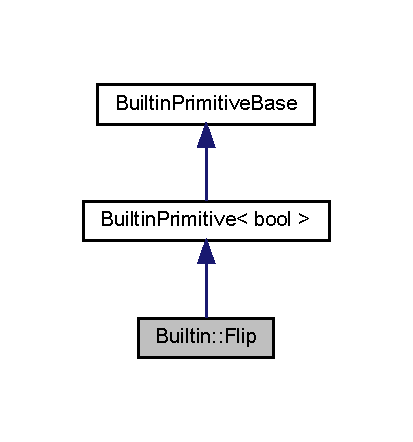
\includegraphics[width=198pt]{struct_builtin_1_1_flip__inherit__graph}
\end{center}
\end{figure}


Collaboration diagram for Builtin\+:\+:Flip\+:
\nopagebreak
\begin{figure}[H]
\begin{center}
\leavevmode
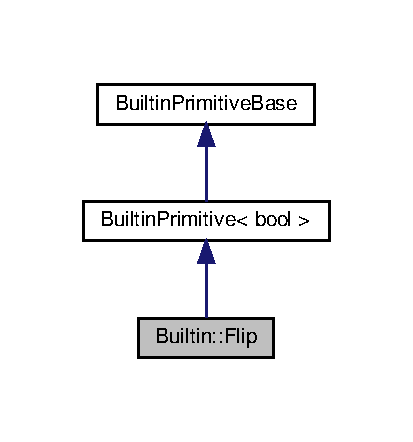
\includegraphics[width=198pt]{struct_builtin_1_1_flip__coll__graph}
\end{center}
\end{figure}
\subsection*{Public Member Functions}
\begin{DoxyCompactItemize}
\item 
\hyperlink{struct_builtin_1_1_flip_a7b2664f6342725c1f1fb91d770b34843}{Flip} (std\+::string fmt, double \+\_\+p=1.\+0)
\end{DoxyCompactItemize}
\subsection*{Additional Inherited Members}


\subsection{Constructor \& Destructor Documentation}
\mbox{\Hypertarget{struct_builtin_1_1_flip_a7b2664f6342725c1f1fb91d770b34843}\label{struct_builtin_1_1_flip_a7b2664f6342725c1f1fb91d770b34843}} 
\index{Builtin\+::\+Flip@{Builtin\+::\+Flip}!Flip@{Flip}}
\index{Flip@{Flip}!Builtin\+::\+Flip@{Builtin\+::\+Flip}}
\subsubsection{\texorpdfstring{Flip()}{Flip()}}
{\footnotesize\ttfamily Builtin\+::\+Flip\+::\+Flip (\begin{DoxyParamCaption}\item[{std\+::string}]{fmt,  }\item[{double}]{\+\_\+p = {\ttfamily 1.0} }\end{DoxyParamCaption})\hspace{0.3cm}{\ttfamily [inline]}}



The documentation for this struct was generated from the following file\+:\begin{DoxyCompactItemize}
\item 
src/\+Virtual\+Machine/\hyperlink{_builtins_8h}{Builtins.\+h}\end{DoxyCompactItemize}

\hypertarget{struct_builtin_1_1_flip_p}{}\doxysection{Builtin\+::FlipP Struct Reference}
\label{struct_builtin_1_1_flip_p}\index{Builtin::FlipP@{Builtin::FlipP}}


{\ttfamily \#include $<$Builtins.\+h$>$}



Inheritance diagram for Builtin\+::FlipP\+:
\nopagebreak
\begin{figure}[H]
\begin{center}
\leavevmode
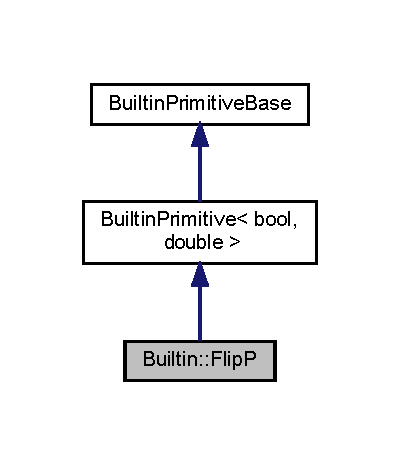
\includegraphics[width=192pt]{struct_builtin_1_1_flip_p__inherit__graph}
\end{center}
\end{figure}


Collaboration diagram for Builtin\+::FlipP\+:
\nopagebreak
\begin{figure}[H]
\begin{center}
\leavevmode
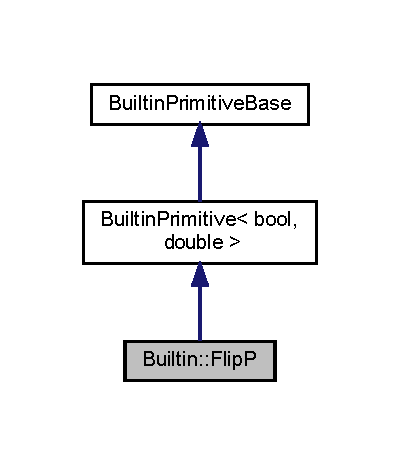
\includegraphics[width=192pt]{struct_builtin_1_1_flip_p__coll__graph}
\end{center}
\end{figure}
\doxysubsection*{Public Member Functions}
\begin{DoxyCompactItemize}
\item 
\mbox{\hyperlink{struct_builtin_1_1_flip_p_adab32b985984688bb906fef95301c7fa}{FlipP}} (std\+::string fmt, double \+\_\+p=1.\+0)
\end{DoxyCompactItemize}
\doxysubsection*{Additional Inherited Members}


\doxysubsection{Constructor \& Destructor Documentation}
\mbox{\Hypertarget{struct_builtin_1_1_flip_p_adab32b985984688bb906fef95301c7fa}\label{struct_builtin_1_1_flip_p_adab32b985984688bb906fef95301c7fa}} 
\index{Builtin::FlipP@{Builtin::FlipP}!FlipP@{FlipP}}
\index{FlipP@{FlipP}!Builtin::FlipP@{Builtin::FlipP}}
\doxysubsubsection{\texorpdfstring{FlipP()}{FlipP()}}
{\footnotesize\ttfamily Builtin\+::\+Flip\+P\+::\+FlipP (\begin{DoxyParamCaption}\item[{std\+::string}]{fmt,  }\item[{double}]{\+\_\+p = {\ttfamily 1.0} }\end{DoxyParamCaption})\hspace{0.3cm}{\ttfamily [inline]}}



The documentation for this struct was generated from the following file\+:\begin{DoxyCompactItemize}
\item 
src/\+Virtual\+Machine/\mbox{\hyperlink{_builtins_8h}{Builtins.\+h}}\end{DoxyCompactItemize}

\hypertarget{class_full_m_c_t_s_node}{}\section{Full\+M\+C\+T\+S\+Node$<$ this\+\_\+t, H\+YP, callback\+\_\+t $>$ Class Template Reference}
\label{class_full_m_c_t_s_node}\index{Full\+M\+C\+T\+S\+Node$<$ this\+\_\+t, H\+Y\+P, callback\+\_\+t $>$@{Full\+M\+C\+T\+S\+Node$<$ this\+\_\+t, H\+Y\+P, callback\+\_\+t $>$}}


{\ttfamily \#include $<$M\+C\+T\+S.\+h$>$}



Inheritance diagram for Full\+M\+C\+T\+S\+Node$<$ this\+\_\+t, H\+YP, callback\+\_\+t $>$\+:
\nopagebreak
\begin{figure}[H]
\begin{center}
\leavevmode
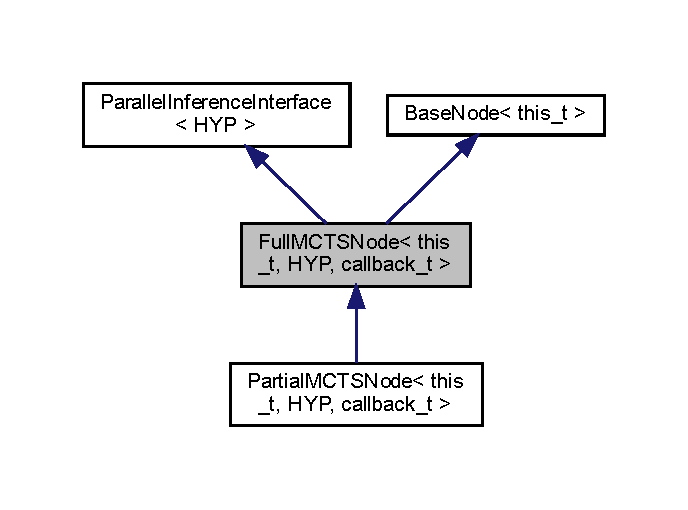
\includegraphics[width=330pt]{class_full_m_c_t_s_node__inherit__graph}
\end{center}
\end{figure}


Collaboration diagram for Full\+M\+C\+T\+S\+Node$<$ this\+\_\+t, H\+YP, callback\+\_\+t $>$\+:
\nopagebreak
\begin{figure}[H]
\begin{center}
\leavevmode
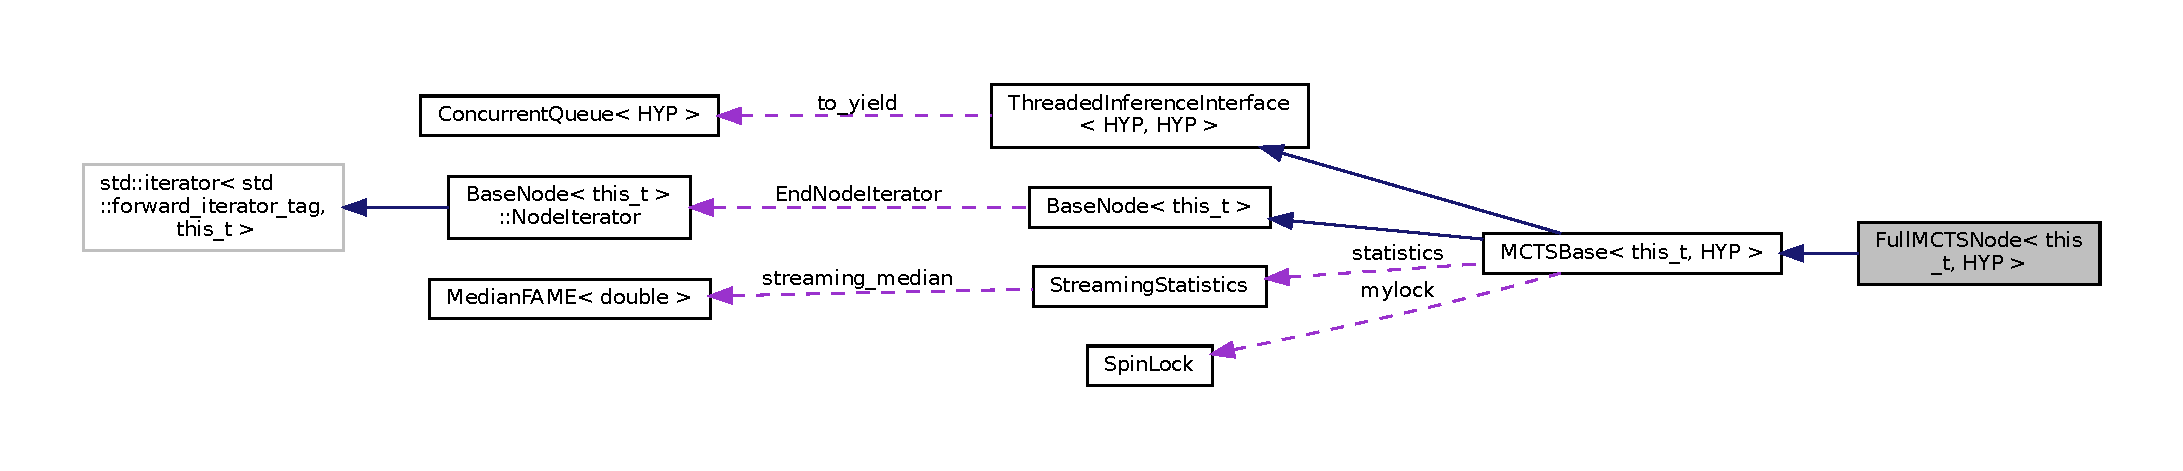
\includegraphics[width=350pt]{class_full_m_c_t_s_node__coll__graph}
\end{center}
\end{figure}
\subsection*{Additional Inherited Members}


\subsection{Detailed Description}
\subsubsection*{template$<$typename this\+\_\+t, typename H\+YP, typename callback\+\_\+t$>$\newline
class Full\+M\+C\+T\+S\+Node$<$ this\+\_\+t, H\+Y\+P, callback\+\_\+t $>$}

\begin{DoxyAuthor}{Author}
Steven Piantadosi 
\end{DoxyAuthor}
\begin{DoxyDate}{Date}
22/12/20 
\end{DoxyDate}


The documentation for this class was generated from the following file\+:\begin{DoxyCompactItemize}
\item 
src/\+Inference/\hyperlink{_m_c_t_s_8h}{M\+C\+T\+S.\+h}\end{DoxyCompactItemize}

\hypertarget{class_grammar}{}\doxysection{Grammar$<$ \+\_\+input\+\_\+t, \+\_\+output\+\_\+t, G\+R\+A\+M\+M\+A\+R\+\_\+\+T\+Y\+P\+ES $>$ Class Template Reference}
\label{class_grammar}\index{Grammar$<$ \_input\_t, \_output\_t, GRAMMAR\_TYPES $>$@{Grammar$<$ \_input\_t, \_output\_t, GRAMMAR\_TYPES $>$}}


{\ttfamily \#include $<$Grammar.\+h$>$}

\doxysubsection*{Classes}
\begin{DoxyCompactItemize}
\item 
class \mbox{\hyperlink{class_grammar_1_1_rule_iterator}{Rule\+Iterator}}
\end{DoxyCompactItemize}
\doxysubsection*{Public Types}
\begin{DoxyCompactItemize}
\item 
using \mbox{\hyperlink{class_grammar_a11116f6d2f48f79def498a97549c67d4}{input\+\_\+t}} = \+\_\+input\+\_\+t
\item 
using \mbox{\hyperlink{class_grammar_aee7630d758322022048d06605b07e697}{output\+\_\+t}} = \+\_\+output\+\_\+t
\item 
using \mbox{\hyperlink{class_grammar_a3193857749e93b641ca05524f94c388e}{this\+\_\+t}} = \mbox{\hyperlink{class_grammar}{Grammar}}$<$ \mbox{\hyperlink{class_grammar_a11116f6d2f48f79def498a97549c67d4}{input\+\_\+t}}, \mbox{\hyperlink{class_grammar_aee7630d758322022048d06605b07e697}{output\+\_\+t}}, G\+R\+A\+M\+M\+A\+R\+\_\+\+T\+Y\+P\+E\+S... $>$
\item 
using \mbox{\hyperlink{class_grammar_abfb390f3654ce837c97c8b3d0d3b5f0f}{Type\+Tuple}} = std\+::tuple$<$ G\+R\+A\+M\+M\+A\+R\+\_\+\+T\+Y\+P\+E\+S... $>$
\item 
using \mbox{\hyperlink{class_grammar_a62e87cde3f753a426cc6688c4dde40b8}{Virtual\+Machine\+State\+\_\+t}} = \mbox{\hyperlink{class_virtual_machine_state}{Virtual\+Machine\+State}}$<$ \mbox{\hyperlink{class_grammar_a11116f6d2f48f79def498a97549c67d4}{input\+\_\+t}}, \mbox{\hyperlink{class_grammar_aee7630d758322022048d06605b07e697}{output\+\_\+t}}, G\+R\+A\+M\+M\+A\+R\+\_\+\+T\+Y\+P\+E\+S... $>$
\item 
using \mbox{\hyperlink{class_grammar_af9b9935f4da29e68087b25ef75f22564}{FT}} = typename \mbox{\hyperlink{class_virtual_machine_state_acacd9869c4a5ff3a765f6bd7d5bae35c}{Virtual\+Machine\+State\+\_\+t\+::\+FT}}
\end{DoxyCompactItemize}
\doxysubsection*{Public Member Functions}
\begin{DoxyCompactItemize}
\item 
\mbox{\hyperlink{class_grammar_aeeaa7bf30a9984e9b2c74b9924856066}{Grammar}} ()
\item 
\mbox{\hyperlink{class_grammar_a0ab84ce4f0bce6a88d73c5d91779fc62}{Grammar}} (const \mbox{\hyperlink{class_grammar}{Grammar}} \&g)=delete
\item 
\mbox{\hyperlink{class_grammar_abfd571fb8e63af1bb50957e70c115cbc}{Grammar}} (const \mbox{\hyperlink{class_grammar}{Grammar}} \&\&g)=delete
\item 
\mbox{\hyperlink{class_grammar_1_1_rule_iterator}{Rule\+Iterator}} \mbox{\hyperlink{class_grammar_aee5716f6501e8a366e33e12c7a675b8d}{begin}} () const
\item 
\mbox{\hyperlink{class_grammar_1_1_rule_iterator}{Rule\+Iterator}} \mbox{\hyperlink{class_grammar_a141508d214bb721b71e8ee27a1aa2915}{end}} () const
\item 
constexpr \mbox{\hyperlink{_nonterminal_8h_a1c5bfe9b903f69c83bbde5da7035fef3}{nonterminal\+\_\+t}} \mbox{\hyperlink{class_grammar_a7126c9e6abbedc4c43047c0ddd2cce5a}{start}} ()
\begin{DoxyCompactList}\small\item\em The start nonterminal type. \end{DoxyCompactList}\item 
constexpr size\+\_\+t \mbox{\hyperlink{class_grammar_ab0bae5bff5a5a8f97116ae49eb6d3a15}{count\+\_\+nonterminals}} () const
\item 
size\+\_\+t \mbox{\hyperlink{class_grammar_acb0ad7c8f130df2dd73bb5040bdf0fa2}{count\+\_\+rules}} (const \mbox{\hyperlink{_nonterminal_8h_a1c5bfe9b903f69c83bbde5da7035fef3}{nonterminal\+\_\+t}} \mbox{\hyperlink{class_grammar_ac7ec043aec5203a2cfac44f9cec50132}{nt}}) const
\item 
size\+\_\+t \mbox{\hyperlink{class_grammar_af6f447aca4141c52f3197eac688c0be7}{count\+\_\+rules}} () const
\item 
size\+\_\+t \mbox{\hyperlink{class_grammar_a44c81f50a71a83e95b558d32fa1715c4}{count\+\_\+terminals}} (\mbox{\hyperlink{_nonterminal_8h_a1c5bfe9b903f69c83bbde5da7035fef3}{nonterminal\+\_\+t}} \mbox{\hyperlink{class_grammar_ac7ec043aec5203a2cfac44f9cec50132}{nt}}) const
\item 
size\+\_\+t \mbox{\hyperlink{class_grammar_acf1de192a73f1c07c44375eb9e08d309}{count\+\_\+nonterminals}} (\mbox{\hyperlink{_nonterminal_8h_a1c5bfe9b903f69c83bbde5da7035fef3}{nonterminal\+\_\+t}} \mbox{\hyperlink{class_grammar_ac7ec043aec5203a2cfac44f9cec50132}{nt}}) const
\item 
{\footnotesize template$<$typename T , typename... args$>$ }\\void \mbox{\hyperlink{class_grammar_af6325e79ee8789f3fe851927f7354d91}{add\+\_\+vms}} (std\+::string fmt, \mbox{\hyperlink{class_grammar_af9b9935f4da29e68087b25ef75f22564}{FT}} $\ast$f, double p=1.\+0, \mbox{\hyperlink{_ops_8h_a588e6b56097e045c733b60d25c4d45ab}{Op}} o=\mbox{\hyperlink{_ops_8h_a588e6b56097e045c733b60d25c4d45abaeb6d8ae6f20283755b339c0dc273988b}{Op\+::\+Standard}}, int a=0)
\item 
{\footnotesize template$<$typename T , typename... args$>$ }\\void \mbox{\hyperlink{class_grammar_a07ae62095abaf00b3da2fc5065c941bf}{add}} (std\+::string fmt, \mbox{\hyperlink{struct_builtin}{Builtin}}$<$ T, args... $>$ b, double p=1.\+0, int a=0)
\item 
{\footnotesize template$<$typename T , typename... args$>$ }\\void \mbox{\hyperlink{class_grammar_a633cc234bdf39f7a875bbb4691ba9470}{add}} (std\+::string fmt, std\+::function$<$ T(args...)$>$ f, double p=1.\+0, \mbox{\hyperlink{_ops_8h_a588e6b56097e045c733b60d25c4d45ab}{Op}} o=\mbox{\hyperlink{_ops_8h_a588e6b56097e045c733b60d25c4d45abaeb6d8ae6f20283755b339c0dc273988b}{Op\+::\+Standard}}, int a=0)
\item 
{\footnotesize template$<$typename T , typename... args$>$ }\\void \mbox{\hyperlink{class_grammar_a29eade7ad059e6e976f7a9c5a607e0b6}{add}} (std\+::string fmt, T($\ast$\+\_\+f)(args...), double p=1.\+0, \mbox{\hyperlink{_ops_8h_a588e6b56097e045c733b60d25c4d45ab}{Op}} o=\mbox{\hyperlink{_ops_8h_a588e6b56097e045c733b60d25c4d45abaeb6d8ae6f20283755b339c0dc273988b}{Op\+::\+Standard}}, int a=0)
\item 
{\footnotesize template$<$typename T $>$ }\\void \mbox{\hyperlink{class_grammar_af43a4d8c3c2c7df80a916a5219b7232c}{add\+\_\+terminal}} (std\+::string fmt, T x, double p=1.\+0, \mbox{\hyperlink{_ops_8h_a588e6b56097e045c733b60d25c4d45ab}{Op}} o=\mbox{\hyperlink{_ops_8h_a588e6b56097e045c733b60d25c4d45abaeb6d8ae6f20283755b339c0dc273988b}{Op\+::\+Standard}}, int a=0)
\begin{DoxyCompactList}\small\item\em Add a variable that is N\+OT A function -- simplification for adding alphabets etc. This just wraps stuff in a thunk for us to make it easier. N\+O\+TE\+: x is copied by value. \end{DoxyCompactList}\item 
size\+\_\+t \mbox{\hyperlink{class_grammar_a4dc14b38ba87cdc516deac5028fa1032}{get\+\_\+index\+\_\+of}} (const \mbox{\hyperlink{class_rule}{Rule}} $\ast$r) const
\item 
virtual \mbox{\hyperlink{class_rule}{Rule}} $\ast$ \mbox{\hyperlink{class_grammar_ad340d2b8ee3b22ff8b697f917a50c0a5}{get\+\_\+rule}} (const \mbox{\hyperlink{_nonterminal_8h_a1c5bfe9b903f69c83bbde5da7035fef3}{nonterminal\+\_\+t}} \mbox{\hyperlink{class_grammar_ac7ec043aec5203a2cfac44f9cec50132}{nt}}, size\+\_\+t k) const
\item 
virtual \mbox{\hyperlink{class_rule}{Rule}} $\ast$ \mbox{\hyperlink{class_grammar_a92123503b80e2c10f0d9b766baf6304f}{get\+\_\+rule}} (const \mbox{\hyperlink{_nonterminal_8h_a1c5bfe9b903f69c83bbde5da7035fef3}{nonterminal\+\_\+t}} \mbox{\hyperlink{class_grammar_ac7ec043aec5203a2cfac44f9cec50132}{nt}}, const \mbox{\hyperlink{_ops_8h_a588e6b56097e045c733b60d25c4d45ab}{Op}} o, const int a=0)
\item 
virtual \mbox{\hyperlink{class_rule}{Rule}} $\ast$ \mbox{\hyperlink{class_grammar_ab2186c76238d843d6ba4242348f0a458}{get\+\_\+rule}} (const \mbox{\hyperlink{_nonterminal_8h_a1c5bfe9b903f69c83bbde5da7035fef3}{nonterminal\+\_\+t}} \mbox{\hyperlink{class_grammar_ac7ec043aec5203a2cfac44f9cec50132}{nt}}, size\+\_\+t i)
\item 
virtual \mbox{\hyperlink{class_rule}{Rule}} $\ast$ \mbox{\hyperlink{class_grammar_ac952ea1ee2eb218622d3db8fa1a5e00f}{get\+\_\+rule}} (const \mbox{\hyperlink{_nonterminal_8h_a1c5bfe9b903f69c83bbde5da7035fef3}{nonterminal\+\_\+t}} \mbox{\hyperlink{class_grammar_ac7ec043aec5203a2cfac44f9cec50132}{nt}}, const std\+::string s) const
\item 
virtual \mbox{\hyperlink{class_rule}{Rule}} $\ast$ \mbox{\hyperlink{class_grammar_a742a677c65f8d14394f5370e8800686d}{get\+\_\+rule}} (const std\+::string s) const
\item 
double \mbox{\hyperlink{class_grammar_a52be4a9de3a90db8034ede12c344e241}{rule\+\_\+normalizer}} (const \mbox{\hyperlink{_nonterminal_8h_a1c5bfe9b903f69c83bbde5da7035fef3}{nonterminal\+\_\+t}} \mbox{\hyperlink{class_grammar_ac7ec043aec5203a2cfac44f9cec50132}{nt}}) const
\item 
virtual \mbox{\hyperlink{class_rule}{Rule}} $\ast$ \mbox{\hyperlink{class_grammar_a427f722a7cc03e06d2ae9321a8b5b757}{sample\+\_\+rule}} (const \mbox{\hyperlink{_nonterminal_8h_a1c5bfe9b903f69c83bbde5da7035fef3}{nonterminal\+\_\+t}} \mbox{\hyperlink{class_grammar_ac7ec043aec5203a2cfac44f9cec50132}{nt}}) const
\item 
\mbox{\hyperlink{class_node}{Node}} \mbox{\hyperlink{class_grammar_aec960301035c8f5f1f8e62338bb3f860}{make\+Node}} (const \mbox{\hyperlink{class_rule}{Rule}} $\ast$r) const
\item 
\mbox{\hyperlink{class_node}{Node}} \mbox{\hyperlink{class_grammar_abbf87abced1821fb1b6a2e1ed43eba74}{generate}} (const \mbox{\hyperlink{_nonterminal_8h_a1c5bfe9b903f69c83bbde5da7035fef3}{nonterminal\+\_\+t}} ntfrom=\mbox{\hyperlink{class_grammar_ac7ec043aec5203a2cfac44f9cec50132}{nt}}$<$ \mbox{\hyperlink{class_grammar_aee7630d758322022048d06605b07e697}{output\+\_\+t}} $>$(), unsigned long depth=0) const
\item 
\mbox{\hyperlink{class_node}{Node}} \mbox{\hyperlink{class_grammar_a9ce6fefd39e27641085efc3ad6a3b077}{copy\+\_\+resample}} (const \mbox{\hyperlink{class_node}{Node}} \&node, bool f(const \mbox{\hyperlink{class_node}{Node}} \&n)) const
\item 
std\+::vector$<$ size\+\_\+t $>$ \mbox{\hyperlink{class_grammar_a842ec663d0131ac6b8175f71cf003ce2}{get\+\_\+cumulative\+\_\+indices}} () const
\item 
std\+::vector$<$ size\+\_\+t $>$ \mbox{\hyperlink{class_grammar_a354a5d9bdaced96748c599bc7c3bd64a}{get\+\_\+counts}} (const \mbox{\hyperlink{class_node}{Node}} \&node) const
\item 
{\footnotesize template$<$typename T $>$ }\\std\+::vector$<$ size\+\_\+t $>$ \mbox{\hyperlink{class_grammar_a336d72ee766941a3ac8c6507c2022a83}{get\+\_\+counts}} (const std\+::vector$<$ T $>$ \&v) const
\item 
double \mbox{\hyperlink{class_grammar_a44385654719beb219184074602ee7440}{log\+\_\+probability}} (const \mbox{\hyperlink{class_node}{Node}} \&n) const
\item 
\mbox{\hyperlink{class_node}{Node}} \mbox{\hyperlink{class_grammar_a63a4c7f6584fdd70aaa2882a19c2f04f}{from\+\_\+parseable}} (std\+::deque$<$ std\+::string $>$ \&q) const
\item 
\mbox{\hyperlink{class_node}{Node}} \mbox{\hyperlink{class_grammar_a55ebb2d60067684f17d721e5ff0cbebf}{from\+\_\+parseable}} (std\+::string s) const
\item 
\mbox{\hyperlink{class_node}{Node}} \mbox{\hyperlink{class_grammar_abd714767f5c9909da54393c638a033e8}{from\+\_\+parseable}} (const char $\ast$c) const
\item 
size\+\_\+t \mbox{\hyperlink{class_grammar_a7026d07264c64f85f370b01b19622415}{neighbors}} (const \mbox{\hyperlink{class_node}{Node}} \&node) const
\item 
void \mbox{\hyperlink{class_grammar_a5849e85e2c5b34174f82f9c784c92fe2}{expand\+\_\+to\+\_\+neighbor}} (\mbox{\hyperlink{class_node}{Node}} \&node, int \&which)
\item 
double \mbox{\hyperlink{class_grammar_a195bd7a052b34884c2e006cbd6ed3c94}{neighbor\+\_\+prior}} (const \mbox{\hyperlink{class_node}{Node}} \&node, int \&which) const
\item 
void \mbox{\hyperlink{class_grammar_a1524560f792f87da632c21f665666d21}{complete}} (\mbox{\hyperlink{class_node}{Node}} \&node)
\end{DoxyCompactItemize}
\doxysubsection*{Static Public Member Functions}
\begin{DoxyCompactItemize}
\item 
{\footnotesize template$<$class T $>$ }\\static constexpr \mbox{\hyperlink{_nonterminal_8h_a1c5bfe9b903f69c83bbde5da7035fef3}{nonterminal\+\_\+t}} \mbox{\hyperlink{class_grammar_ac7ec043aec5203a2cfac44f9cec50132}{nt}} ()
\item 
{\footnotesize template$<$typename X $>$ }\\static constexpr bool \mbox{\hyperlink{class_grammar_a09dff6ea6759e21aced0f655b496a93a}{is\+\_\+in\+\_\+\+G\+R\+A\+M\+M\+A\+R\+\_\+\+T\+Y\+P\+ES}} ()
\begin{DoxyCompactList}\small\item\em For a given nt, returns the number of finite trees that nt can expand to if its finite; 0 if its infinite. $\ast$ ~\newline
 \end{DoxyCompactList}\end{DoxyCompactItemize}
\doxysubsection*{Public Attributes}
\begin{DoxyCompactItemize}
\item 
std\+::vector$<$ \mbox{\hyperlink{class_rule}{Rule}} $>$ \mbox{\hyperlink{class_grammar_a06752487e61dd790df43b530044702fd}{rules}} \mbox{[}\mbox{\hyperlink{class_grammar_a845af53585cb7b104458b4f4b6da114f}{N\+\_\+\+N\+Ts}}\mbox{]}
\item 
std\+::array$<$ double, \mbox{\hyperlink{class_grammar_a845af53585cb7b104458b4f4b6da114f}{N\+\_\+\+N\+Ts}} $>$ \mbox{\hyperlink{class_grammar_a7cf38380ce1e0ea85706673859693d71}{Z}}
\item 
size\+\_\+t \mbox{\hyperlink{class_grammar_a87c7974198d014c9fd324fbfd39b62e6}{G\+R\+A\+M\+M\+A\+R\+\_\+\+M\+A\+X\+\_\+\+D\+E\+P\+TH}} = 64
\end{DoxyCompactItemize}
\doxysubsection*{Static Public Attributes}
\begin{DoxyCompactItemize}
\item 
static constexpr size\+\_\+t \mbox{\hyperlink{class_grammar_a845af53585cb7b104458b4f4b6da114f}{N\+\_\+\+N\+Ts}} = std\+::tuple\+\_\+size$<$\mbox{\hyperlink{class_grammar_abfb390f3654ce837c97c8b3d0d3b5f0f}{Type\+Tuple}}$>$\+::value
\end{DoxyCompactItemize}


\doxysubsection{Detailed Description}
\subsubsection*{template$<$typename \+\_\+input\+\_\+t, typename \+\_\+output\+\_\+t, typename... G\+R\+A\+M\+M\+A\+R\+\_\+\+T\+Y\+P\+ES$>$\newline
class Grammar$<$ \+\_\+input\+\_\+t, \+\_\+output\+\_\+t, G\+R\+A\+M\+M\+A\+R\+\_\+\+T\+Y\+P\+E\+S $>$}

\begin{DoxyAuthor}{Author}
Steven Piantadosi 
\end{DoxyAuthor}
\begin{DoxyDate}{Date}
05/09/20 
\end{DoxyDate}


\doxysubsection{Member Typedef Documentation}
\mbox{\Hypertarget{class_grammar_af9b9935f4da29e68087b25ef75f22564}\label{class_grammar_af9b9935f4da29e68087b25ef75f22564}} 
\index{Grammar$<$ \_input\_t, \_output\_t, GRAMMAR\_TYPES $>$@{Grammar$<$ \_input\_t, \_output\_t, GRAMMAR\_TYPES $>$}!FT@{FT}}
\index{FT@{FT}!Grammar$<$ \_input\_t, \_output\_t, GRAMMAR\_TYPES $>$@{Grammar$<$ \_input\_t, \_output\_t, GRAMMAR\_TYPES $>$}}
\doxysubsubsection{\texorpdfstring{FT}{FT}}
{\footnotesize\ttfamily template$<$typename \+\_\+input\+\_\+t , typename \+\_\+output\+\_\+t , typename... G\+R\+A\+M\+M\+A\+R\+\_\+\+T\+Y\+P\+ES$>$ \\
using \mbox{\hyperlink{class_grammar}{Grammar}}$<$ \+\_\+input\+\_\+t, \+\_\+output\+\_\+t, G\+R\+A\+M\+M\+A\+R\+\_\+\+T\+Y\+P\+ES $>$\+::\mbox{\hyperlink{class_grammar_af9b9935f4da29e68087b25ef75f22564}{FT}} =  typename \mbox{\hyperlink{class_virtual_machine_state_acacd9869c4a5ff3a765f6bd7d5bae35c}{Virtual\+Machine\+State\+\_\+t\+::\+FT}}}

\mbox{\Hypertarget{class_grammar_a11116f6d2f48f79def498a97549c67d4}\label{class_grammar_a11116f6d2f48f79def498a97549c67d4}} 
\index{Grammar$<$ \_input\_t, \_output\_t, GRAMMAR\_TYPES $>$@{Grammar$<$ \_input\_t, \_output\_t, GRAMMAR\_TYPES $>$}!input\_t@{input\_t}}
\index{input\_t@{input\_t}!Grammar$<$ \_input\_t, \_output\_t, GRAMMAR\_TYPES $>$@{Grammar$<$ \_input\_t, \_output\_t, GRAMMAR\_TYPES $>$}}
\doxysubsubsection{\texorpdfstring{input\_t}{input\_t}}
{\footnotesize\ttfamily template$<$typename \+\_\+input\+\_\+t , typename \+\_\+output\+\_\+t , typename... G\+R\+A\+M\+M\+A\+R\+\_\+\+T\+Y\+P\+ES$>$ \\
using \mbox{\hyperlink{class_grammar}{Grammar}}$<$ \+\_\+input\+\_\+t, \+\_\+output\+\_\+t, G\+R\+A\+M\+M\+A\+R\+\_\+\+T\+Y\+P\+ES $>$\+::\mbox{\hyperlink{class_grammar_a11116f6d2f48f79def498a97549c67d4}{input\+\_\+t}} =  \+\_\+input\+\_\+t}

\mbox{\Hypertarget{class_grammar_aee7630d758322022048d06605b07e697}\label{class_grammar_aee7630d758322022048d06605b07e697}} 
\index{Grammar$<$ \_input\_t, \_output\_t, GRAMMAR\_TYPES $>$@{Grammar$<$ \_input\_t, \_output\_t, GRAMMAR\_TYPES $>$}!output\_t@{output\_t}}
\index{output\_t@{output\_t}!Grammar$<$ \_input\_t, \_output\_t, GRAMMAR\_TYPES $>$@{Grammar$<$ \_input\_t, \_output\_t, GRAMMAR\_TYPES $>$}}
\doxysubsubsection{\texorpdfstring{output\_t}{output\_t}}
{\footnotesize\ttfamily template$<$typename \+\_\+input\+\_\+t , typename \+\_\+output\+\_\+t , typename... G\+R\+A\+M\+M\+A\+R\+\_\+\+T\+Y\+P\+ES$>$ \\
using \mbox{\hyperlink{class_grammar}{Grammar}}$<$ \+\_\+input\+\_\+t, \+\_\+output\+\_\+t, G\+R\+A\+M\+M\+A\+R\+\_\+\+T\+Y\+P\+ES $>$\+::\mbox{\hyperlink{class_grammar_aee7630d758322022048d06605b07e697}{output\+\_\+t}} =  \+\_\+output\+\_\+t}

\mbox{\Hypertarget{class_grammar_a3193857749e93b641ca05524f94c388e}\label{class_grammar_a3193857749e93b641ca05524f94c388e}} 
\index{Grammar$<$ \_input\_t, \_output\_t, GRAMMAR\_TYPES $>$@{Grammar$<$ \_input\_t, \_output\_t, GRAMMAR\_TYPES $>$}!this\_t@{this\_t}}
\index{this\_t@{this\_t}!Grammar$<$ \_input\_t, \_output\_t, GRAMMAR\_TYPES $>$@{Grammar$<$ \_input\_t, \_output\_t, GRAMMAR\_TYPES $>$}}
\doxysubsubsection{\texorpdfstring{this\_t}{this\_t}}
{\footnotesize\ttfamily template$<$typename \+\_\+input\+\_\+t , typename \+\_\+output\+\_\+t , typename... G\+R\+A\+M\+M\+A\+R\+\_\+\+T\+Y\+P\+ES$>$ \\
using \mbox{\hyperlink{class_grammar}{Grammar}}$<$ \+\_\+input\+\_\+t, \+\_\+output\+\_\+t, G\+R\+A\+M\+M\+A\+R\+\_\+\+T\+Y\+P\+ES $>$\+::\mbox{\hyperlink{class_grammar_a3193857749e93b641ca05524f94c388e}{this\+\_\+t}} =  \mbox{\hyperlink{class_grammar}{Grammar}}$<$\mbox{\hyperlink{class_grammar_a11116f6d2f48f79def498a97549c67d4}{input\+\_\+t}}, \mbox{\hyperlink{class_grammar_aee7630d758322022048d06605b07e697}{output\+\_\+t}}, G\+R\+A\+M\+M\+A\+R\+\_\+\+T\+Y\+P\+E\+S...$>$}

\mbox{\Hypertarget{class_grammar_abfb390f3654ce837c97c8b3d0d3b5f0f}\label{class_grammar_abfb390f3654ce837c97c8b3d0d3b5f0f}} 
\index{Grammar$<$ \_input\_t, \_output\_t, GRAMMAR\_TYPES $>$@{Grammar$<$ \_input\_t, \_output\_t, GRAMMAR\_TYPES $>$}!TypeTuple@{TypeTuple}}
\index{TypeTuple@{TypeTuple}!Grammar$<$ \_input\_t, \_output\_t, GRAMMAR\_TYPES $>$@{Grammar$<$ \_input\_t, \_output\_t, GRAMMAR\_TYPES $>$}}
\doxysubsubsection{\texorpdfstring{TypeTuple}{TypeTuple}}
{\footnotesize\ttfamily template$<$typename \+\_\+input\+\_\+t , typename \+\_\+output\+\_\+t , typename... G\+R\+A\+M\+M\+A\+R\+\_\+\+T\+Y\+P\+ES$>$ \\
using \mbox{\hyperlink{class_grammar}{Grammar}}$<$ \+\_\+input\+\_\+t, \+\_\+output\+\_\+t, G\+R\+A\+M\+M\+A\+R\+\_\+\+T\+Y\+P\+ES $>$\+::\mbox{\hyperlink{class_grammar_abfb390f3654ce837c97c8b3d0d3b5f0f}{Type\+Tuple}} =  std\+::tuple$<$G\+R\+A\+M\+M\+A\+R\+\_\+\+T\+Y\+P\+E\+S...$>$}

\mbox{\Hypertarget{class_grammar_a62e87cde3f753a426cc6688c4dde40b8}\label{class_grammar_a62e87cde3f753a426cc6688c4dde40b8}} 
\index{Grammar$<$ \_input\_t, \_output\_t, GRAMMAR\_TYPES $>$@{Grammar$<$ \_input\_t, \_output\_t, GRAMMAR\_TYPES $>$}!VirtualMachineState\_t@{VirtualMachineState\_t}}
\index{VirtualMachineState\_t@{VirtualMachineState\_t}!Grammar$<$ \_input\_t, \_output\_t, GRAMMAR\_TYPES $>$@{Grammar$<$ \_input\_t, \_output\_t, GRAMMAR\_TYPES $>$}}
\doxysubsubsection{\texorpdfstring{VirtualMachineState\_t}{VirtualMachineState\_t}}
{\footnotesize\ttfamily template$<$typename \+\_\+input\+\_\+t , typename \+\_\+output\+\_\+t , typename... G\+R\+A\+M\+M\+A\+R\+\_\+\+T\+Y\+P\+ES$>$ \\
using \mbox{\hyperlink{class_grammar}{Grammar}}$<$ \+\_\+input\+\_\+t, \+\_\+output\+\_\+t, G\+R\+A\+M\+M\+A\+R\+\_\+\+T\+Y\+P\+ES $>$\+::\mbox{\hyperlink{class_grammar_a62e87cde3f753a426cc6688c4dde40b8}{Virtual\+Machine\+State\+\_\+t}} =  \mbox{\hyperlink{class_virtual_machine_state}{Virtual\+Machine\+State}}$<$\mbox{\hyperlink{class_grammar_a11116f6d2f48f79def498a97549c67d4}{input\+\_\+t}}, \mbox{\hyperlink{class_grammar_aee7630d758322022048d06605b07e697}{output\+\_\+t}}, G\+R\+A\+M\+M\+A\+R\+\_\+\+T\+Y\+P\+E\+S...$>$}



\doxysubsection{Constructor \& Destructor Documentation}
\mbox{\Hypertarget{class_grammar_aeeaa7bf30a9984e9b2c74b9924856066}\label{class_grammar_aeeaa7bf30a9984e9b2c74b9924856066}} 
\index{Grammar$<$ \_input\_t, \_output\_t, GRAMMAR\_TYPES $>$@{Grammar$<$ \_input\_t, \_output\_t, GRAMMAR\_TYPES $>$}!Grammar@{Grammar}}
\index{Grammar@{Grammar}!Grammar$<$ \_input\_t, \_output\_t, GRAMMAR\_TYPES $>$@{Grammar$<$ \_input\_t, \_output\_t, GRAMMAR\_TYPES $>$}}
\doxysubsubsection{\texorpdfstring{Grammar()}{Grammar()}\hspace{0.1cm}{\footnotesize\ttfamily [1/3]}}
{\footnotesize\ttfamily template$<$typename \+\_\+input\+\_\+t , typename \+\_\+output\+\_\+t , typename... G\+R\+A\+M\+M\+A\+R\+\_\+\+T\+Y\+P\+ES$>$ \\
\mbox{\hyperlink{class_grammar}{Grammar}}$<$ \+\_\+input\+\_\+t, \+\_\+output\+\_\+t, G\+R\+A\+M\+M\+A\+R\+\_\+\+T\+Y\+P\+ES $>$\+::\mbox{\hyperlink{class_grammar}{Grammar}} (\begin{DoxyParamCaption}{ }\end{DoxyParamCaption})\hspace{0.3cm}{\ttfamily [inline]}}

\mbox{\Hypertarget{class_grammar_a0ab84ce4f0bce6a88d73c5d91779fc62}\label{class_grammar_a0ab84ce4f0bce6a88d73c5d91779fc62}} 
\index{Grammar$<$ \_input\_t, \_output\_t, GRAMMAR\_TYPES $>$@{Grammar$<$ \_input\_t, \_output\_t, GRAMMAR\_TYPES $>$}!Grammar@{Grammar}}
\index{Grammar@{Grammar}!Grammar$<$ \_input\_t, \_output\_t, GRAMMAR\_TYPES $>$@{Grammar$<$ \_input\_t, \_output\_t, GRAMMAR\_TYPES $>$}}
\doxysubsubsection{\texorpdfstring{Grammar()}{Grammar()}\hspace{0.1cm}{\footnotesize\ttfamily [2/3]}}
{\footnotesize\ttfamily template$<$typename \+\_\+input\+\_\+t , typename \+\_\+output\+\_\+t , typename... G\+R\+A\+M\+M\+A\+R\+\_\+\+T\+Y\+P\+ES$>$ \\
\mbox{\hyperlink{class_grammar}{Grammar}}$<$ \+\_\+input\+\_\+t, \+\_\+output\+\_\+t, G\+R\+A\+M\+M\+A\+R\+\_\+\+T\+Y\+P\+ES $>$\+::\mbox{\hyperlink{class_grammar}{Grammar}} (\begin{DoxyParamCaption}\item[{const \mbox{\hyperlink{class_grammar}{Grammar}}$<$ \+\_\+input\+\_\+t, \+\_\+output\+\_\+t, G\+R\+A\+M\+M\+A\+R\+\_\+\+T\+Y\+P\+ES $>$ \&}]{g }\end{DoxyParamCaption})\hspace{0.3cm}{\ttfamily [delete]}}

\mbox{\Hypertarget{class_grammar_abfd571fb8e63af1bb50957e70c115cbc}\label{class_grammar_abfd571fb8e63af1bb50957e70c115cbc}} 
\index{Grammar$<$ \_input\_t, \_output\_t, GRAMMAR\_TYPES $>$@{Grammar$<$ \_input\_t, \_output\_t, GRAMMAR\_TYPES $>$}!Grammar@{Grammar}}
\index{Grammar@{Grammar}!Grammar$<$ \_input\_t, \_output\_t, GRAMMAR\_TYPES $>$@{Grammar$<$ \_input\_t, \_output\_t, GRAMMAR\_TYPES $>$}}
\doxysubsubsection{\texorpdfstring{Grammar()}{Grammar()}\hspace{0.1cm}{\footnotesize\ttfamily [3/3]}}
{\footnotesize\ttfamily template$<$typename \+\_\+input\+\_\+t , typename \+\_\+output\+\_\+t , typename... G\+R\+A\+M\+M\+A\+R\+\_\+\+T\+Y\+P\+ES$>$ \\
\mbox{\hyperlink{class_grammar}{Grammar}}$<$ \+\_\+input\+\_\+t, \+\_\+output\+\_\+t, G\+R\+A\+M\+M\+A\+R\+\_\+\+T\+Y\+P\+ES $>$\+::\mbox{\hyperlink{class_grammar}{Grammar}} (\begin{DoxyParamCaption}\item[{const \mbox{\hyperlink{class_grammar}{Grammar}}$<$ \+\_\+input\+\_\+t, \+\_\+output\+\_\+t, G\+R\+A\+M\+M\+A\+R\+\_\+\+T\+Y\+P\+ES $>$ \&\&}]{g }\end{DoxyParamCaption})\hspace{0.3cm}{\ttfamily [delete]}}



\doxysubsection{Member Function Documentation}
\mbox{\Hypertarget{class_grammar_a07ae62095abaf00b3da2fc5065c941bf}\label{class_grammar_a07ae62095abaf00b3da2fc5065c941bf}} 
\index{Grammar$<$ \_input\_t, \_output\_t, GRAMMAR\_TYPES $>$@{Grammar$<$ \_input\_t, \_output\_t, GRAMMAR\_TYPES $>$}!add@{add}}
\index{add@{add}!Grammar$<$ \_input\_t, \_output\_t, GRAMMAR\_TYPES $>$@{Grammar$<$ \_input\_t, \_output\_t, GRAMMAR\_TYPES $>$}}
\doxysubsubsection{\texorpdfstring{add()}{add()}\hspace{0.1cm}{\footnotesize\ttfamily [1/3]}}
{\footnotesize\ttfamily template$<$typename \+\_\+input\+\_\+t , typename \+\_\+output\+\_\+t , typename... G\+R\+A\+M\+M\+A\+R\+\_\+\+T\+Y\+P\+ES$>$ \\
template$<$typename T , typename... args$>$ \\
void \mbox{\hyperlink{class_grammar}{Grammar}}$<$ \+\_\+input\+\_\+t, \+\_\+output\+\_\+t, G\+R\+A\+M\+M\+A\+R\+\_\+\+T\+Y\+P\+ES $>$\+::add (\begin{DoxyParamCaption}\item[{std\+::string}]{fmt,  }\item[{\mbox{\hyperlink{struct_builtin}{Builtin}}$<$ T, args... $>$}]{b,  }\item[{double}]{p = {\ttfamily 1.0},  }\item[{int}]{a = {\ttfamily 0} }\end{DoxyParamCaption})\hspace{0.3cm}{\ttfamily [inline]}}


\begin{DoxyParams}{Parameters}
{\em fmt} & \\
\hline
{\em b} & \\
\hline
{\em p} & \\
\hline
\end{DoxyParams}
\mbox{\Hypertarget{class_grammar_a633cc234bdf39f7a875bbb4691ba9470}\label{class_grammar_a633cc234bdf39f7a875bbb4691ba9470}} 
\index{Grammar$<$ \_input\_t, \_output\_t, GRAMMAR\_TYPES $>$@{Grammar$<$ \_input\_t, \_output\_t, GRAMMAR\_TYPES $>$}!add@{add}}
\index{add@{add}!Grammar$<$ \_input\_t, \_output\_t, GRAMMAR\_TYPES $>$@{Grammar$<$ \_input\_t, \_output\_t, GRAMMAR\_TYPES $>$}}
\doxysubsubsection{\texorpdfstring{add()}{add()}\hspace{0.1cm}{\footnotesize\ttfamily [2/3]}}
{\footnotesize\ttfamily template$<$typename \+\_\+input\+\_\+t , typename \+\_\+output\+\_\+t , typename... G\+R\+A\+M\+M\+A\+R\+\_\+\+T\+Y\+P\+ES$>$ \\
template$<$typename T , typename... args$>$ \\
void \mbox{\hyperlink{class_grammar}{Grammar}}$<$ \+\_\+input\+\_\+t, \+\_\+output\+\_\+t, G\+R\+A\+M\+M\+A\+R\+\_\+\+T\+Y\+P\+ES $>$\+::add (\begin{DoxyParamCaption}\item[{std\+::string}]{fmt,  }\item[{std\+::function$<$ T(args...)$>$}]{f,  }\item[{double}]{p = {\ttfamily 1.0},  }\item[{\mbox{\hyperlink{_ops_8h_a588e6b56097e045c733b60d25c4d45ab}{Op}}}]{o = {\ttfamily \mbox{\hyperlink{_ops_8h_a588e6b56097e045c733b60d25c4d45abaeb6d8ae6f20283755b339c0dc273988b}{Op\+::\+Standard}}},  }\item[{int}]{a = {\ttfamily 0} }\end{DoxyParamCaption})\hspace{0.3cm}{\ttfamily [inline]}}


\begin{DoxyParams}{Parameters}
{\em fmt} & \\
\hline
{\em f} & \\
\hline
{\em p} & \\
\hline
{\em o} & \\
\hline
\end{DoxyParams}
\mbox{\Hypertarget{class_grammar_a29eade7ad059e6e976f7a9c5a607e0b6}\label{class_grammar_a29eade7ad059e6e976f7a9c5a607e0b6}} 
\index{Grammar$<$ \_input\_t, \_output\_t, GRAMMAR\_TYPES $>$@{Grammar$<$ \_input\_t, \_output\_t, GRAMMAR\_TYPES $>$}!add@{add}}
\index{add@{add}!Grammar$<$ \_input\_t, \_output\_t, GRAMMAR\_TYPES $>$@{Grammar$<$ \_input\_t, \_output\_t, GRAMMAR\_TYPES $>$}}
\doxysubsubsection{\texorpdfstring{add()}{add()}\hspace{0.1cm}{\footnotesize\ttfamily [3/3]}}
{\footnotesize\ttfamily template$<$typename \+\_\+input\+\_\+t , typename \+\_\+output\+\_\+t , typename... G\+R\+A\+M\+M\+A\+R\+\_\+\+T\+Y\+P\+ES$>$ \\
template$<$typename T , typename... args$>$ \\
void \mbox{\hyperlink{class_grammar}{Grammar}}$<$ \+\_\+input\+\_\+t, \+\_\+output\+\_\+t, G\+R\+A\+M\+M\+A\+R\+\_\+\+T\+Y\+P\+ES $>$\+::add (\begin{DoxyParamCaption}\item[{std\+::string}]{fmt,  }\item[{T($\ast$)(args...)}]{\+\_\+f,  }\item[{double}]{p = {\ttfamily 1.0},  }\item[{\mbox{\hyperlink{_ops_8h_a588e6b56097e045c733b60d25c4d45ab}{Op}}}]{o = {\ttfamily \mbox{\hyperlink{_ops_8h_a588e6b56097e045c733b60d25c4d45abaeb6d8ae6f20283755b339c0dc273988b}{Op\+::\+Standard}}},  }\item[{int}]{a = {\ttfamily 0} }\end{DoxyParamCaption})\hspace{0.3cm}{\ttfamily [inline]}}


\begin{DoxyParams}{Parameters}
{\em fmt} & \\
\hline
{\em p} & \\
\hline
{\em o} & \\
\hline
\end{DoxyParams}
\mbox{\Hypertarget{class_grammar_af43a4d8c3c2c7df80a916a5219b7232c}\label{class_grammar_af43a4d8c3c2c7df80a916a5219b7232c}} 
\index{Grammar$<$ \_input\_t, \_output\_t, GRAMMAR\_TYPES $>$@{Grammar$<$ \_input\_t, \_output\_t, GRAMMAR\_TYPES $>$}!add\_terminal@{add\_terminal}}
\index{add\_terminal@{add\_terminal}!Grammar$<$ \_input\_t, \_output\_t, GRAMMAR\_TYPES $>$@{Grammar$<$ \_input\_t, \_output\_t, GRAMMAR\_TYPES $>$}}
\doxysubsubsection{\texorpdfstring{add\_terminal()}{add\_terminal()}}
{\footnotesize\ttfamily template$<$typename \+\_\+input\+\_\+t , typename \+\_\+output\+\_\+t , typename... G\+R\+A\+M\+M\+A\+R\+\_\+\+T\+Y\+P\+ES$>$ \\
template$<$typename T $>$ \\
void \mbox{\hyperlink{class_grammar}{Grammar}}$<$ \+\_\+input\+\_\+t, \+\_\+output\+\_\+t, G\+R\+A\+M\+M\+A\+R\+\_\+\+T\+Y\+P\+ES $>$\+::add\+\_\+terminal (\begin{DoxyParamCaption}\item[{std\+::string}]{fmt,  }\item[{T}]{x,  }\item[{double}]{p = {\ttfamily 1.0},  }\item[{\mbox{\hyperlink{_ops_8h_a588e6b56097e045c733b60d25c4d45ab}{Op}}}]{o = {\ttfamily \mbox{\hyperlink{_ops_8h_a588e6b56097e045c733b60d25c4d45abaeb6d8ae6f20283755b339c0dc273988b}{Op\+::\+Standard}}},  }\item[{int}]{a = {\ttfamily 0} }\end{DoxyParamCaption})\hspace{0.3cm}{\ttfamily [inline]}}



Add a variable that is N\+OT A function -- simplification for adding alphabets etc. This just wraps stuff in a thunk for us to make it easier. N\+O\+TE\+: x is copied by value. 


\begin{DoxyParams}{Parameters}
{\em fmt} & \\
\hline
{\em x} & \\
\hline
{\em p} & \\
\hline
{\em o} & \\
\hline
{\em a} & \\
\hline
\end{DoxyParams}
\mbox{\Hypertarget{class_grammar_af6325e79ee8789f3fe851927f7354d91}\label{class_grammar_af6325e79ee8789f3fe851927f7354d91}} 
\index{Grammar$<$ \_input\_t, \_output\_t, GRAMMAR\_TYPES $>$@{Grammar$<$ \_input\_t, \_output\_t, GRAMMAR\_TYPES $>$}!add\_vms@{add\_vms}}
\index{add\_vms@{add\_vms}!Grammar$<$ \_input\_t, \_output\_t, GRAMMAR\_TYPES $>$@{Grammar$<$ \_input\_t, \_output\_t, GRAMMAR\_TYPES $>$}}
\doxysubsubsection{\texorpdfstring{add\_vms()}{add\_vms()}}
{\footnotesize\ttfamily template$<$typename \+\_\+input\+\_\+t , typename \+\_\+output\+\_\+t , typename... G\+R\+A\+M\+M\+A\+R\+\_\+\+T\+Y\+P\+ES$>$ \\
template$<$typename T , typename... args$>$ \\
void \mbox{\hyperlink{class_grammar}{Grammar}}$<$ \+\_\+input\+\_\+t, \+\_\+output\+\_\+t, G\+R\+A\+M\+M\+A\+R\+\_\+\+T\+Y\+P\+ES $>$\+::add\+\_\+vms (\begin{DoxyParamCaption}\item[{std\+::string}]{fmt,  }\item[{\mbox{\hyperlink{class_grammar_af9b9935f4da29e68087b25ef75f22564}{FT}} $\ast$}]{f,  }\item[{double}]{p = {\ttfamily 1.0},  }\item[{\mbox{\hyperlink{_ops_8h_a588e6b56097e045c733b60d25c4d45ab}{Op}}}]{o = {\ttfamily \mbox{\hyperlink{_ops_8h_a588e6b56097e045c733b60d25c4d45abaeb6d8ae6f20283755b339c0dc273988b}{Op\+::\+Standard}}},  }\item[{int}]{a = {\ttfamily 0} }\end{DoxyParamCaption})\hspace{0.3cm}{\ttfamily [inline]}}


\begin{DoxyParams}{Parameters}
{\em fmt} & \\
\hline
{\em f} & \\
\hline
{\em p} & \\
\hline
{\em o} & \\
\hline
\end{DoxyParams}
\mbox{\Hypertarget{class_grammar_aee5716f6501e8a366e33e12c7a675b8d}\label{class_grammar_aee5716f6501e8a366e33e12c7a675b8d}} 
\index{Grammar$<$ \_input\_t, \_output\_t, GRAMMAR\_TYPES $>$@{Grammar$<$ \_input\_t, \_output\_t, GRAMMAR\_TYPES $>$}!begin@{begin}}
\index{begin@{begin}!Grammar$<$ \_input\_t, \_output\_t, GRAMMAR\_TYPES $>$@{Grammar$<$ \_input\_t, \_output\_t, GRAMMAR\_TYPES $>$}}
\doxysubsubsection{\texorpdfstring{begin()}{begin()}}
{\footnotesize\ttfamily template$<$typename \+\_\+input\+\_\+t , typename \+\_\+output\+\_\+t , typename... G\+R\+A\+M\+M\+A\+R\+\_\+\+T\+Y\+P\+ES$>$ \\
\mbox{\hyperlink{class_grammar_1_1_rule_iterator}{Rule\+Iterator}} \mbox{\hyperlink{class_grammar}{Grammar}}$<$ \+\_\+input\+\_\+t, \+\_\+output\+\_\+t, G\+R\+A\+M\+M\+A\+R\+\_\+\+T\+Y\+P\+ES $>$\+::begin (\begin{DoxyParamCaption}{ }\end{DoxyParamCaption}) const\hspace{0.3cm}{\ttfamily [inline]}}

\mbox{\Hypertarget{class_grammar_a1524560f792f87da632c21f665666d21}\label{class_grammar_a1524560f792f87da632c21f665666d21}} 
\index{Grammar$<$ \_input\_t, \_output\_t, GRAMMAR\_TYPES $>$@{Grammar$<$ \_input\_t, \_output\_t, GRAMMAR\_TYPES $>$}!complete@{complete}}
\index{complete@{complete}!Grammar$<$ \_input\_t, \_output\_t, GRAMMAR\_TYPES $>$@{Grammar$<$ \_input\_t, \_output\_t, GRAMMAR\_TYPES $>$}}
\doxysubsubsection{\texorpdfstring{complete()}{complete()}}
{\footnotesize\ttfamily template$<$typename \+\_\+input\+\_\+t , typename \+\_\+output\+\_\+t , typename... G\+R\+A\+M\+M\+A\+R\+\_\+\+T\+Y\+P\+ES$>$ \\
void \mbox{\hyperlink{class_grammar}{Grammar}}$<$ \+\_\+input\+\_\+t, \+\_\+output\+\_\+t, G\+R\+A\+M\+M\+A\+R\+\_\+\+T\+Y\+P\+ES $>$\+::complete (\begin{DoxyParamCaption}\item[{\mbox{\hyperlink{class_node}{Node}} \&}]{node }\end{DoxyParamCaption})\hspace{0.3cm}{\ttfamily [inline]}}

\mbox{\Hypertarget{class_grammar_a9ce6fefd39e27641085efc3ad6a3b077}\label{class_grammar_a9ce6fefd39e27641085efc3ad6a3b077}} 
\index{Grammar$<$ \_input\_t, \_output\_t, GRAMMAR\_TYPES $>$@{Grammar$<$ \_input\_t, \_output\_t, GRAMMAR\_TYPES $>$}!copy\_resample@{copy\_resample}}
\index{copy\_resample@{copy\_resample}!Grammar$<$ \_input\_t, \_output\_t, GRAMMAR\_TYPES $>$@{Grammar$<$ \_input\_t, \_output\_t, GRAMMAR\_TYPES $>$}}
\doxysubsubsection{\texorpdfstring{copy\_resample()}{copy\_resample()}}
{\footnotesize\ttfamily template$<$typename \+\_\+input\+\_\+t , typename \+\_\+output\+\_\+t , typename... G\+R\+A\+M\+M\+A\+R\+\_\+\+T\+Y\+P\+ES$>$ \\
\mbox{\hyperlink{class_node}{Node}} \mbox{\hyperlink{class_grammar}{Grammar}}$<$ \+\_\+input\+\_\+t, \+\_\+output\+\_\+t, G\+R\+A\+M\+M\+A\+R\+\_\+\+T\+Y\+P\+ES $>$\+::copy\+\_\+resample (\begin{DoxyParamCaption}\item[{const \mbox{\hyperlink{class_node}{Node}} \&}]{node,  }\item[{bool }]{fconst Node \&n }\end{DoxyParamCaption}) const\hspace{0.3cm}{\ttfamily [inline]}}

Make a copy of node where all nodes satisfying f are regenerated from the grammar. 
\begin{DoxyParams}{Parameters}
{\em node} & \\
\hline
{\em f} & -\/ a function saying what we should resample \\
\hline
\end{DoxyParams}
\begin{DoxyReturn}{Returns}
N\+O\+TE\+: this does N\+OT allow f to apply to nullptr children (so cannot be used to fill in)
\end{DoxyReturn}
\mbox{\Hypertarget{class_grammar_ab0bae5bff5a5a8f97116ae49eb6d3a15}\label{class_grammar_ab0bae5bff5a5a8f97116ae49eb6d3a15}} 
\index{Grammar$<$ \_input\_t, \_output\_t, GRAMMAR\_TYPES $>$@{Grammar$<$ \_input\_t, \_output\_t, GRAMMAR\_TYPES $>$}!count\_nonterminals@{count\_nonterminals}}
\index{count\_nonterminals@{count\_nonterminals}!Grammar$<$ \_input\_t, \_output\_t, GRAMMAR\_TYPES $>$@{Grammar$<$ \_input\_t, \_output\_t, GRAMMAR\_TYPES $>$}}
\doxysubsubsection{\texorpdfstring{count\_nonterminals()}{count\_nonterminals()}\hspace{0.1cm}{\footnotesize\ttfamily [1/2]}}
{\footnotesize\ttfamily template$<$typename \+\_\+input\+\_\+t , typename \+\_\+output\+\_\+t , typename... G\+R\+A\+M\+M\+A\+R\+\_\+\+T\+Y\+P\+ES$>$ \\
constexpr size\+\_\+t \mbox{\hyperlink{class_grammar}{Grammar}}$<$ \+\_\+input\+\_\+t, \+\_\+output\+\_\+t, G\+R\+A\+M\+M\+A\+R\+\_\+\+T\+Y\+P\+ES $>$\+::count\+\_\+nonterminals (\begin{DoxyParamCaption}{ }\end{DoxyParamCaption}) const\hspace{0.3cm}{\ttfamily [inline]}, {\ttfamily [constexpr]}}

How many nonterminals are there in the grammar. \begin{DoxyReturn}{Returns}

\end{DoxyReturn}
\mbox{\Hypertarget{class_grammar_acf1de192a73f1c07c44375eb9e08d309}\label{class_grammar_acf1de192a73f1c07c44375eb9e08d309}} 
\index{Grammar$<$ \_input\_t, \_output\_t, GRAMMAR\_TYPES $>$@{Grammar$<$ \_input\_t, \_output\_t, GRAMMAR\_TYPES $>$}!count\_nonterminals@{count\_nonterminals}}
\index{count\_nonterminals@{count\_nonterminals}!Grammar$<$ \_input\_t, \_output\_t, GRAMMAR\_TYPES $>$@{Grammar$<$ \_input\_t, \_output\_t, GRAMMAR\_TYPES $>$}}
\doxysubsubsection{\texorpdfstring{count\_nonterminals()}{count\_nonterminals()}\hspace{0.1cm}{\footnotesize\ttfamily [2/2]}}
{\footnotesize\ttfamily template$<$typename \+\_\+input\+\_\+t , typename \+\_\+output\+\_\+t , typename... G\+R\+A\+M\+M\+A\+R\+\_\+\+T\+Y\+P\+ES$>$ \\
size\+\_\+t \mbox{\hyperlink{class_grammar}{Grammar}}$<$ \+\_\+input\+\_\+t, \+\_\+output\+\_\+t, G\+R\+A\+M\+M\+A\+R\+\_\+\+T\+Y\+P\+ES $>$\+::count\+\_\+nonterminals (\begin{DoxyParamCaption}\item[{\mbox{\hyperlink{_nonterminal_8h_a1c5bfe9b903f69c83bbde5da7035fef3}{nonterminal\+\_\+t}}}]{nt }\end{DoxyParamCaption}) const\hspace{0.3cm}{\ttfamily [inline]}}

Count th enumber of non-\/terminal rules of return type nt 
\begin{DoxyParams}{Parameters}
{\em nt} & \\
\hline
\end{DoxyParams}
\begin{DoxyReturn}{Returns}

\end{DoxyReturn}
\mbox{\Hypertarget{class_grammar_af6f447aca4141c52f3197eac688c0be7}\label{class_grammar_af6f447aca4141c52f3197eac688c0be7}} 
\index{Grammar$<$ \_input\_t, \_output\_t, GRAMMAR\_TYPES $>$@{Grammar$<$ \_input\_t, \_output\_t, GRAMMAR\_TYPES $>$}!count\_rules@{count\_rules}}
\index{count\_rules@{count\_rules}!Grammar$<$ \_input\_t, \_output\_t, GRAMMAR\_TYPES $>$@{Grammar$<$ \_input\_t, \_output\_t, GRAMMAR\_TYPES $>$}}
\doxysubsubsection{\texorpdfstring{count\_rules()}{count\_rules()}\hspace{0.1cm}{\footnotesize\ttfamily [1/2]}}
{\footnotesize\ttfamily template$<$typename \+\_\+input\+\_\+t , typename \+\_\+output\+\_\+t , typename... G\+R\+A\+M\+M\+A\+R\+\_\+\+T\+Y\+P\+ES$>$ \\
size\+\_\+t \mbox{\hyperlink{class_grammar}{Grammar}}$<$ \+\_\+input\+\_\+t, \+\_\+output\+\_\+t, G\+R\+A\+M\+M\+A\+R\+\_\+\+T\+Y\+P\+ES $>$\+::count\+\_\+rules (\begin{DoxyParamCaption}{ }\end{DoxyParamCaption}) const\hspace{0.3cm}{\ttfamily [inline]}}

Total number of rules \begin{DoxyReturn}{Returns}

\end{DoxyReturn}
\mbox{\Hypertarget{class_grammar_acb0ad7c8f130df2dd73bb5040bdf0fa2}\label{class_grammar_acb0ad7c8f130df2dd73bb5040bdf0fa2}} 
\index{Grammar$<$ \_input\_t, \_output\_t, GRAMMAR\_TYPES $>$@{Grammar$<$ \_input\_t, \_output\_t, GRAMMAR\_TYPES $>$}!count\_rules@{count\_rules}}
\index{count\_rules@{count\_rules}!Grammar$<$ \_input\_t, \_output\_t, GRAMMAR\_TYPES $>$@{Grammar$<$ \_input\_t, \_output\_t, GRAMMAR\_TYPES $>$}}
\doxysubsubsection{\texorpdfstring{count\_rules()}{count\_rules()}\hspace{0.1cm}{\footnotesize\ttfamily [2/2]}}
{\footnotesize\ttfamily template$<$typename \+\_\+input\+\_\+t , typename \+\_\+output\+\_\+t , typename... G\+R\+A\+M\+M\+A\+R\+\_\+\+T\+Y\+P\+ES$>$ \\
size\+\_\+t \mbox{\hyperlink{class_grammar}{Grammar}}$<$ \+\_\+input\+\_\+t, \+\_\+output\+\_\+t, G\+R\+A\+M\+M\+A\+R\+\_\+\+T\+Y\+P\+ES $>$\+::count\+\_\+rules (\begin{DoxyParamCaption}\item[{const \mbox{\hyperlink{_nonterminal_8h_a1c5bfe9b903f69c83bbde5da7035fef3}{nonterminal\+\_\+t}}}]{nt }\end{DoxyParamCaption}) const\hspace{0.3cm}{\ttfamily [inline]}}

Returns the number of rules of return type nt 
\begin{DoxyParams}{Parameters}
{\em nt} & \\
\hline
\end{DoxyParams}
\begin{DoxyReturn}{Returns}

\end{DoxyReturn}
\mbox{\Hypertarget{class_grammar_a44c81f50a71a83e95b558d32fa1715c4}\label{class_grammar_a44c81f50a71a83e95b558d32fa1715c4}} 
\index{Grammar$<$ \_input\_t, \_output\_t, GRAMMAR\_TYPES $>$@{Grammar$<$ \_input\_t, \_output\_t, GRAMMAR\_TYPES $>$}!count\_terminals@{count\_terminals}}
\index{count\_terminals@{count\_terminals}!Grammar$<$ \_input\_t, \_output\_t, GRAMMAR\_TYPES $>$@{Grammar$<$ \_input\_t, \_output\_t, GRAMMAR\_TYPES $>$}}
\doxysubsubsection{\texorpdfstring{count\_terminals()}{count\_terminals()}}
{\footnotesize\ttfamily template$<$typename \+\_\+input\+\_\+t , typename \+\_\+output\+\_\+t , typename... G\+R\+A\+M\+M\+A\+R\+\_\+\+T\+Y\+P\+ES$>$ \\
size\+\_\+t \mbox{\hyperlink{class_grammar}{Grammar}}$<$ \+\_\+input\+\_\+t, \+\_\+output\+\_\+t, G\+R\+A\+M\+M\+A\+R\+\_\+\+T\+Y\+P\+ES $>$\+::count\+\_\+terminals (\begin{DoxyParamCaption}\item[{\mbox{\hyperlink{_nonterminal_8h_a1c5bfe9b903f69c83bbde5da7035fef3}{nonterminal\+\_\+t}}}]{nt }\end{DoxyParamCaption}) const\hspace{0.3cm}{\ttfamily [inline]}}

Count the number of terminal rules of return type nt 
\begin{DoxyParams}{Parameters}
{\em nt} & \\
\hline
\end{DoxyParams}
\begin{DoxyReturn}{Returns}

\end{DoxyReturn}
\mbox{\Hypertarget{class_grammar_a141508d214bb721b71e8ee27a1aa2915}\label{class_grammar_a141508d214bb721b71e8ee27a1aa2915}} 
\index{Grammar$<$ \_input\_t, \_output\_t, GRAMMAR\_TYPES $>$@{Grammar$<$ \_input\_t, \_output\_t, GRAMMAR\_TYPES $>$}!end@{end}}
\index{end@{end}!Grammar$<$ \_input\_t, \_output\_t, GRAMMAR\_TYPES $>$@{Grammar$<$ \_input\_t, \_output\_t, GRAMMAR\_TYPES $>$}}
\doxysubsubsection{\texorpdfstring{end()}{end()}}
{\footnotesize\ttfamily template$<$typename \+\_\+input\+\_\+t , typename \+\_\+output\+\_\+t , typename... G\+R\+A\+M\+M\+A\+R\+\_\+\+T\+Y\+P\+ES$>$ \\
\mbox{\hyperlink{class_grammar_1_1_rule_iterator}{Rule\+Iterator}} \mbox{\hyperlink{class_grammar}{Grammar}}$<$ \+\_\+input\+\_\+t, \+\_\+output\+\_\+t, G\+R\+A\+M\+M\+A\+R\+\_\+\+T\+Y\+P\+ES $>$\+::end (\begin{DoxyParamCaption}{ }\end{DoxyParamCaption}) const\hspace{0.3cm}{\ttfamily [inline]}}

\mbox{\Hypertarget{class_grammar_a5849e85e2c5b34174f82f9c784c92fe2}\label{class_grammar_a5849e85e2c5b34174f82f9c784c92fe2}} 
\index{Grammar$<$ \_input\_t, \_output\_t, GRAMMAR\_TYPES $>$@{Grammar$<$ \_input\_t, \_output\_t, GRAMMAR\_TYPES $>$}!expand\_to\_neighbor@{expand\_to\_neighbor}}
\index{expand\_to\_neighbor@{expand\_to\_neighbor}!Grammar$<$ \_input\_t, \_output\_t, GRAMMAR\_TYPES $>$@{Grammar$<$ \_input\_t, \_output\_t, GRAMMAR\_TYPES $>$}}
\doxysubsubsection{\texorpdfstring{expand\_to\_neighbor()}{expand\_to\_neighbor()}}
{\footnotesize\ttfamily template$<$typename \+\_\+input\+\_\+t , typename \+\_\+output\+\_\+t , typename... G\+R\+A\+M\+M\+A\+R\+\_\+\+T\+Y\+P\+ES$>$ \\
void \mbox{\hyperlink{class_grammar}{Grammar}}$<$ \+\_\+input\+\_\+t, \+\_\+output\+\_\+t, G\+R\+A\+M\+M\+A\+R\+\_\+\+T\+Y\+P\+ES $>$\+::expand\+\_\+to\+\_\+neighbor (\begin{DoxyParamCaption}\item[{\mbox{\hyperlink{class_node}{Node}} \&}]{node,  }\item[{int \&}]{which }\end{DoxyParamCaption})\hspace{0.3cm}{\ttfamily [inline]}}

\mbox{\Hypertarget{class_grammar_abd714767f5c9909da54393c638a033e8}\label{class_grammar_abd714767f5c9909da54393c638a033e8}} 
\index{Grammar$<$ \_input\_t, \_output\_t, GRAMMAR\_TYPES $>$@{Grammar$<$ \_input\_t, \_output\_t, GRAMMAR\_TYPES $>$}!from\_parseable@{from\_parseable}}
\index{from\_parseable@{from\_parseable}!Grammar$<$ \_input\_t, \_output\_t, GRAMMAR\_TYPES $>$@{Grammar$<$ \_input\_t, \_output\_t, GRAMMAR\_TYPES $>$}}
\doxysubsubsection{\texorpdfstring{from\_parseable()}{from\_parseable()}\hspace{0.1cm}{\footnotesize\ttfamily [1/3]}}
{\footnotesize\ttfamily template$<$typename \+\_\+input\+\_\+t , typename \+\_\+output\+\_\+t , typename... G\+R\+A\+M\+M\+A\+R\+\_\+\+T\+Y\+P\+ES$>$ \\
\mbox{\hyperlink{class_node}{Node}} \mbox{\hyperlink{class_grammar}{Grammar}}$<$ \+\_\+input\+\_\+t, \+\_\+output\+\_\+t, G\+R\+A\+M\+M\+A\+R\+\_\+\+T\+Y\+P\+ES $>$\+::from\+\_\+parseable (\begin{DoxyParamCaption}\item[{const char $\ast$}]{c }\end{DoxyParamCaption}) const\hspace{0.3cm}{\ttfamily [inline]}}

\mbox{\Hypertarget{class_grammar_a63a4c7f6584fdd70aaa2882a19c2f04f}\label{class_grammar_a63a4c7f6584fdd70aaa2882a19c2f04f}} 
\index{Grammar$<$ \_input\_t, \_output\_t, GRAMMAR\_TYPES $>$@{Grammar$<$ \_input\_t, \_output\_t, GRAMMAR\_TYPES $>$}!from\_parseable@{from\_parseable}}
\index{from\_parseable@{from\_parseable}!Grammar$<$ \_input\_t, \_output\_t, GRAMMAR\_TYPES $>$@{Grammar$<$ \_input\_t, \_output\_t, GRAMMAR\_TYPES $>$}}
\doxysubsubsection{\texorpdfstring{from\_parseable()}{from\_parseable()}\hspace{0.1cm}{\footnotesize\ttfamily [2/3]}}
{\footnotesize\ttfamily template$<$typename \+\_\+input\+\_\+t , typename \+\_\+output\+\_\+t , typename... G\+R\+A\+M\+M\+A\+R\+\_\+\+T\+Y\+P\+ES$>$ \\
\mbox{\hyperlink{class_node}{Node}} \mbox{\hyperlink{class_grammar}{Grammar}}$<$ \+\_\+input\+\_\+t, \+\_\+output\+\_\+t, G\+R\+A\+M\+M\+A\+R\+\_\+\+T\+Y\+P\+ES $>$\+::from\+\_\+parseable (\begin{DoxyParamCaption}\item[{std\+::deque$<$ std\+::string $>$ \&}]{q }\end{DoxyParamCaption}) const\hspace{0.3cm}{\ttfamily [inline]}}

Fills an entire tree using the string format prefixes -- see get\+\_\+rule(std\+::string). Here q should contain strings like \char`\"{}3\+:\textquotesingle{}a\textquotesingle{}\char`\"{} which says expand nonterminal type 3 to the rule matching \textquotesingle{}a\textquotesingle{} N\+O\+TE\+: This is not a \mbox{\hyperlink{class_serializable}{Serializable}} interface because the \mbox{\hyperlink{class_node}{Node}} needs to know which grammar 
\begin{DoxyParams}{Parameters}
{\em q} & \\
\hline
\end{DoxyParams}
\begin{DoxyReturn}{Returns}

\end{DoxyReturn}
\mbox{\Hypertarget{class_grammar_a55ebb2d60067684f17d721e5ff0cbebf}\label{class_grammar_a55ebb2d60067684f17d721e5ff0cbebf}} 
\index{Grammar$<$ \_input\_t, \_output\_t, GRAMMAR\_TYPES $>$@{Grammar$<$ \_input\_t, \_output\_t, GRAMMAR\_TYPES $>$}!from\_parseable@{from\_parseable}}
\index{from\_parseable@{from\_parseable}!Grammar$<$ \_input\_t, \_output\_t, GRAMMAR\_TYPES $>$@{Grammar$<$ \_input\_t, \_output\_t, GRAMMAR\_TYPES $>$}}
\doxysubsubsection{\texorpdfstring{from\_parseable()}{from\_parseable()}\hspace{0.1cm}{\footnotesize\ttfamily [3/3]}}
{\footnotesize\ttfamily template$<$typename \+\_\+input\+\_\+t , typename \+\_\+output\+\_\+t , typename... G\+R\+A\+M\+M\+A\+R\+\_\+\+T\+Y\+P\+ES$>$ \\
\mbox{\hyperlink{class_node}{Node}} \mbox{\hyperlink{class_grammar}{Grammar}}$<$ \+\_\+input\+\_\+t, \+\_\+output\+\_\+t, G\+R\+A\+M\+M\+A\+R\+\_\+\+T\+Y\+P\+ES $>$\+::from\+\_\+parseable (\begin{DoxyParamCaption}\item[{std\+::string}]{s }\end{DoxyParamCaption}) const\hspace{0.3cm}{\ttfamily [inline]}}

Expand from names where s is delimited by \textquotesingle{}\+:\textquotesingle{} 
\begin{DoxyParams}{Parameters}
{\em s} & \\
\hline
\end{DoxyParams}
\begin{DoxyReturn}{Returns}

\end{DoxyReturn}
\mbox{\Hypertarget{class_grammar_abbf87abced1821fb1b6a2e1ed43eba74}\label{class_grammar_abbf87abced1821fb1b6a2e1ed43eba74}} 
\index{Grammar$<$ \_input\_t, \_output\_t, GRAMMAR\_TYPES $>$@{Grammar$<$ \_input\_t, \_output\_t, GRAMMAR\_TYPES $>$}!generate@{generate}}
\index{generate@{generate}!Grammar$<$ \_input\_t, \_output\_t, GRAMMAR\_TYPES $>$@{Grammar$<$ \_input\_t, \_output\_t, GRAMMAR\_TYPES $>$}}
\doxysubsubsection{\texorpdfstring{generate()}{generate()}}
{\footnotesize\ttfamily template$<$typename \+\_\+input\+\_\+t , typename \+\_\+output\+\_\+t , typename... G\+R\+A\+M\+M\+A\+R\+\_\+\+T\+Y\+P\+ES$>$ \\
\mbox{\hyperlink{class_node}{Node}} \mbox{\hyperlink{class_grammar}{Grammar}}$<$ \+\_\+input\+\_\+t, \+\_\+output\+\_\+t, G\+R\+A\+M\+M\+A\+R\+\_\+\+T\+Y\+P\+ES $>$\+::generate (\begin{DoxyParamCaption}\item[{const \mbox{\hyperlink{_nonterminal_8h_a1c5bfe9b903f69c83bbde5da7035fef3}{nonterminal\+\_\+t}}}]{ntfrom = {\ttfamily \mbox{\hyperlink{class_grammar_ac7ec043aec5203a2cfac44f9cec50132}{nt}}$<$\mbox{\hyperlink{class_grammar_aee7630d758322022048d06605b07e697}{output\+\_\+t}}$>$()},  }\item[{unsigned long}]{depth = {\ttfamily 0} }\end{DoxyParamCaption}) const\hspace{0.3cm}{\ttfamily [inline]}}

Sample an entire tree from this grammar (keeping track of depth in case we recurse too far) of return type nt. This samples a rule, makes them with make\+Node, and then recurses. 
\begin{DoxyParams}{Parameters}
{\em nt} & \\
\hline
{\em depth} & \\
\hline
\end{DoxyParams}
\begin{DoxyReturn}{Returns}
Returns a \mbox{\hyperlink{class_node}{Node}} sampled from the grammar.
\end{DoxyReturn}
N\+O\+TE\+: this may throw a if the grammar recurses too far (usually that means the grammar is improper)\mbox{\Hypertarget{class_grammar_a354a5d9bdaced96748c599bc7c3bd64a}\label{class_grammar_a354a5d9bdaced96748c599bc7c3bd64a}} 
\index{Grammar$<$ \_input\_t, \_output\_t, GRAMMAR\_TYPES $>$@{Grammar$<$ \_input\_t, \_output\_t, GRAMMAR\_TYPES $>$}!get\_counts@{get\_counts}}
\index{get\_counts@{get\_counts}!Grammar$<$ \_input\_t, \_output\_t, GRAMMAR\_TYPES $>$@{Grammar$<$ \_input\_t, \_output\_t, GRAMMAR\_TYPES $>$}}
\doxysubsubsection{\texorpdfstring{get\_counts()}{get\_counts()}\hspace{0.1cm}{\footnotesize\ttfamily [1/2]}}
{\footnotesize\ttfamily template$<$typename \+\_\+input\+\_\+t , typename \+\_\+output\+\_\+t , typename... G\+R\+A\+M\+M\+A\+R\+\_\+\+T\+Y\+P\+ES$>$ \\
std\+::vector$<$size\+\_\+t$>$ \mbox{\hyperlink{class_grammar}{Grammar}}$<$ \+\_\+input\+\_\+t, \+\_\+output\+\_\+t, G\+R\+A\+M\+M\+A\+R\+\_\+\+T\+Y\+P\+ES $>$\+::get\+\_\+counts (\begin{DoxyParamCaption}\item[{const \mbox{\hyperlink{class_node}{Node}} \&}]{node }\end{DoxyParamCaption}) const\hspace{0.3cm}{\ttfamily [inline]}}

Compute a vector of counts of how often each rule was used, in a {\itshape standard} order given by iterating over nts and then iterating over rules 
\begin{DoxyParams}{Parameters}
{\em node} & \\
\hline
\end{DoxyParams}
\begin{DoxyReturn}{Returns}

\end{DoxyReturn}
\mbox{\Hypertarget{class_grammar_a336d72ee766941a3ac8c6507c2022a83}\label{class_grammar_a336d72ee766941a3ac8c6507c2022a83}} 
\index{Grammar$<$ \_input\_t, \_output\_t, GRAMMAR\_TYPES $>$@{Grammar$<$ \_input\_t, \_output\_t, GRAMMAR\_TYPES $>$}!get\_counts@{get\_counts}}
\index{get\_counts@{get\_counts}!Grammar$<$ \_input\_t, \_output\_t, GRAMMAR\_TYPES $>$@{Grammar$<$ \_input\_t, \_output\_t, GRAMMAR\_TYPES $>$}}
\doxysubsubsection{\texorpdfstring{get\_counts()}{get\_counts()}\hspace{0.1cm}{\footnotesize\ttfamily [2/2]}}
{\footnotesize\ttfamily template$<$typename \+\_\+input\+\_\+t , typename \+\_\+output\+\_\+t , typename... G\+R\+A\+M\+M\+A\+R\+\_\+\+T\+Y\+P\+ES$>$ \\
template$<$typename T $>$ \\
std\+::vector$<$size\+\_\+t$>$ \mbox{\hyperlink{class_grammar}{Grammar}}$<$ \+\_\+input\+\_\+t, \+\_\+output\+\_\+t, G\+R\+A\+M\+M\+A\+R\+\_\+\+T\+Y\+P\+ES $>$\+::get\+\_\+counts (\begin{DoxyParamCaption}\item[{const std\+::vector$<$ T $>$ \&}]{v }\end{DoxyParamCaption}) const\hspace{0.3cm}{\ttfamily [inline]}}

Compute a vector of counts of how often each rule was used, in a {\itshape standard} order given by iterating over nts and then iterating over rules 
\begin{DoxyParams}{Parameters}
{\em v} & \\
\hline
\end{DoxyParams}
\begin{DoxyReturn}{Returns}

\end{DoxyReturn}
\mbox{\Hypertarget{class_grammar_a842ec663d0131ac6b8175f71cf003ce2}\label{class_grammar_a842ec663d0131ac6b8175f71cf003ce2}} 
\index{Grammar$<$ \_input\_t, \_output\_t, GRAMMAR\_TYPES $>$@{Grammar$<$ \_input\_t, \_output\_t, GRAMMAR\_TYPES $>$}!get\_cumulative\_indices@{get\_cumulative\_indices}}
\index{get\_cumulative\_indices@{get\_cumulative\_indices}!Grammar$<$ \_input\_t, \_output\_t, GRAMMAR\_TYPES $>$@{Grammar$<$ \_input\_t, \_output\_t, GRAMMAR\_TYPES $>$}}
\doxysubsubsection{\texorpdfstring{get\_cumulative\_indices()}{get\_cumulative\_indices()}}
{\footnotesize\ttfamily template$<$typename \+\_\+input\+\_\+t , typename \+\_\+output\+\_\+t , typename... G\+R\+A\+M\+M\+A\+R\+\_\+\+T\+Y\+P\+ES$>$ \\
std\+::vector$<$size\+\_\+t$>$ \mbox{\hyperlink{class_grammar}{Grammar}}$<$ \+\_\+input\+\_\+t, \+\_\+output\+\_\+t, G\+R\+A\+M\+M\+A\+R\+\_\+\+T\+Y\+P\+ES $>$\+::get\+\_\+cumulative\+\_\+indices (\begin{DoxyParamCaption}{ }\end{DoxyParamCaption}) const\hspace{0.3cm}{\ttfamily [inline]}}

\mbox{\Hypertarget{class_grammar_a4dc14b38ba87cdc516deac5028fa1032}\label{class_grammar_a4dc14b38ba87cdc516deac5028fa1032}} 
\index{Grammar$<$ \_input\_t, \_output\_t, GRAMMAR\_TYPES $>$@{Grammar$<$ \_input\_t, \_output\_t, GRAMMAR\_TYPES $>$}!get\_index\_of@{get\_index\_of}}
\index{get\_index\_of@{get\_index\_of}!Grammar$<$ \_input\_t, \_output\_t, GRAMMAR\_TYPES $>$@{Grammar$<$ \_input\_t, \_output\_t, GRAMMAR\_TYPES $>$}}
\doxysubsubsection{\texorpdfstring{get\_index\_of()}{get\_index\_of()}}
{\footnotesize\ttfamily template$<$typename \+\_\+input\+\_\+t , typename \+\_\+output\+\_\+t , typename... G\+R\+A\+M\+M\+A\+R\+\_\+\+T\+Y\+P\+ES$>$ \\
size\+\_\+t \mbox{\hyperlink{class_grammar}{Grammar}}$<$ \+\_\+input\+\_\+t, \+\_\+output\+\_\+t, G\+R\+A\+M\+M\+A\+R\+\_\+\+T\+Y\+P\+ES $>$\+::get\+\_\+index\+\_\+of (\begin{DoxyParamCaption}\item[{const \mbox{\hyperlink{class_rule}{Rule}} $\ast$}]{r }\end{DoxyParamCaption}) const\hspace{0.3cm}{\ttfamily [inline]}}

Find the index in rules of where r is. 
\begin{DoxyParams}{Parameters}
{\em r} & \\
\hline
\end{DoxyParams}
\begin{DoxyReturn}{Returns}

\end{DoxyReturn}
\mbox{\Hypertarget{class_grammar_a92123503b80e2c10f0d9b766baf6304f}\label{class_grammar_a92123503b80e2c10f0d9b766baf6304f}} 
\index{Grammar$<$ \_input\_t, \_output\_t, GRAMMAR\_TYPES $>$@{Grammar$<$ \_input\_t, \_output\_t, GRAMMAR\_TYPES $>$}!get\_rule@{get\_rule}}
\index{get\_rule@{get\_rule}!Grammar$<$ \_input\_t, \_output\_t, GRAMMAR\_TYPES $>$@{Grammar$<$ \_input\_t, \_output\_t, GRAMMAR\_TYPES $>$}}
\doxysubsubsection{\texorpdfstring{get\_rule()}{get\_rule()}\hspace{0.1cm}{\footnotesize\ttfamily [1/5]}}
{\footnotesize\ttfamily template$<$typename \+\_\+input\+\_\+t , typename \+\_\+output\+\_\+t , typename... G\+R\+A\+M\+M\+A\+R\+\_\+\+T\+Y\+P\+ES$>$ \\
virtual \mbox{\hyperlink{class_rule}{Rule}}$\ast$ \mbox{\hyperlink{class_grammar}{Grammar}}$<$ \+\_\+input\+\_\+t, \+\_\+output\+\_\+t, G\+R\+A\+M\+M\+A\+R\+\_\+\+T\+Y\+P\+ES $>$\+::get\+\_\+rule (\begin{DoxyParamCaption}\item[{const \mbox{\hyperlink{_nonterminal_8h_a1c5bfe9b903f69c83bbde5da7035fef3}{nonterminal\+\_\+t}}}]{nt,  }\item[{const \mbox{\hyperlink{_ops_8h_a588e6b56097e045c733b60d25c4d45ab}{Op}}}]{o,  }\item[{const int}]{a = {\ttfamily 0} }\end{DoxyParamCaption})\hspace{0.3cm}{\ttfamily [inline]}, {\ttfamily [virtual]}}

Get rule of type nt with a given Builtin\+Op and argument a 
\begin{DoxyParams}{Parameters}
{\em nt} & \\
\hline
{\em o} & \\
\hline
{\em a} & \\
\hline
\end{DoxyParams}
\begin{DoxyReturn}{Returns}

\end{DoxyReturn}
\mbox{\Hypertarget{class_grammar_ac952ea1ee2eb218622d3db8fa1a5e00f}\label{class_grammar_ac952ea1ee2eb218622d3db8fa1a5e00f}} 
\index{Grammar$<$ \_input\_t, \_output\_t, GRAMMAR\_TYPES $>$@{Grammar$<$ \_input\_t, \_output\_t, GRAMMAR\_TYPES $>$}!get\_rule@{get\_rule}}
\index{get\_rule@{get\_rule}!Grammar$<$ \_input\_t, \_output\_t, GRAMMAR\_TYPES $>$@{Grammar$<$ \_input\_t, \_output\_t, GRAMMAR\_TYPES $>$}}
\doxysubsubsection{\texorpdfstring{get\_rule()}{get\_rule()}\hspace{0.1cm}{\footnotesize\ttfamily [2/5]}}
{\footnotesize\ttfamily template$<$typename \+\_\+input\+\_\+t , typename \+\_\+output\+\_\+t , typename... G\+R\+A\+M\+M\+A\+R\+\_\+\+T\+Y\+P\+ES$>$ \\
virtual \mbox{\hyperlink{class_rule}{Rule}}$\ast$ \mbox{\hyperlink{class_grammar}{Grammar}}$<$ \+\_\+input\+\_\+t, \+\_\+output\+\_\+t, G\+R\+A\+M\+M\+A\+R\+\_\+\+T\+Y\+P\+ES $>$\+::get\+\_\+rule (\begin{DoxyParamCaption}\item[{const \mbox{\hyperlink{_nonterminal_8h_a1c5bfe9b903f69c83bbde5da7035fef3}{nonterminal\+\_\+t}}}]{nt,  }\item[{const std\+::string}]{s }\end{DoxyParamCaption}) const\hspace{0.3cm}{\ttfamily [inline]}, {\ttfamily [virtual]}}

Return a rule based on s, which must uniquely be a prefix of the rule\textquotesingle{}s format of a given nonterminal type. If s is the empty string, however, it must match exactly. 
\begin{DoxyParams}{Parameters}
{\em s} & \\
\hline
\end{DoxyParams}
\begin{DoxyReturn}{Returns}

\end{DoxyReturn}
\mbox{\Hypertarget{class_grammar_ab2186c76238d843d6ba4242348f0a458}\label{class_grammar_ab2186c76238d843d6ba4242348f0a458}} 
\index{Grammar$<$ \_input\_t, \_output\_t, GRAMMAR\_TYPES $>$@{Grammar$<$ \_input\_t, \_output\_t, GRAMMAR\_TYPES $>$}!get\_rule@{get\_rule}}
\index{get\_rule@{get\_rule}!Grammar$<$ \_input\_t, \_output\_t, GRAMMAR\_TYPES $>$@{Grammar$<$ \_input\_t, \_output\_t, GRAMMAR\_TYPES $>$}}
\doxysubsubsection{\texorpdfstring{get\_rule()}{get\_rule()}\hspace{0.1cm}{\footnotesize\ttfamily [3/5]}}
{\footnotesize\ttfamily template$<$typename \+\_\+input\+\_\+t , typename \+\_\+output\+\_\+t , typename... G\+R\+A\+M\+M\+A\+R\+\_\+\+T\+Y\+P\+ES$>$ \\
virtual \mbox{\hyperlink{class_rule}{Rule}}$\ast$ \mbox{\hyperlink{class_grammar}{Grammar}}$<$ \+\_\+input\+\_\+t, \+\_\+output\+\_\+t, G\+R\+A\+M\+M\+A\+R\+\_\+\+T\+Y\+P\+ES $>$\+::get\+\_\+rule (\begin{DoxyParamCaption}\item[{const \mbox{\hyperlink{_nonterminal_8h_a1c5bfe9b903f69c83bbde5da7035fef3}{nonterminal\+\_\+t}}}]{nt,  }\item[{size\+\_\+t}]{i }\end{DoxyParamCaption})\hspace{0.3cm}{\ttfamily [inline]}, {\ttfamily [virtual]}}

\mbox{\Hypertarget{class_grammar_ad340d2b8ee3b22ff8b697f917a50c0a5}\label{class_grammar_ad340d2b8ee3b22ff8b697f917a50c0a5}} 
\index{Grammar$<$ \_input\_t, \_output\_t, GRAMMAR\_TYPES $>$@{Grammar$<$ \_input\_t, \_output\_t, GRAMMAR\_TYPES $>$}!get\_rule@{get\_rule}}
\index{get\_rule@{get\_rule}!Grammar$<$ \_input\_t, \_output\_t, GRAMMAR\_TYPES $>$@{Grammar$<$ \_input\_t, \_output\_t, GRAMMAR\_TYPES $>$}}
\doxysubsubsection{\texorpdfstring{get\_rule()}{get\_rule()}\hspace{0.1cm}{\footnotesize\ttfamily [4/5]}}
{\footnotesize\ttfamily template$<$typename \+\_\+input\+\_\+t , typename \+\_\+output\+\_\+t , typename... G\+R\+A\+M\+M\+A\+R\+\_\+\+T\+Y\+P\+ES$>$ \\
virtual \mbox{\hyperlink{class_rule}{Rule}}$\ast$ \mbox{\hyperlink{class_grammar}{Grammar}}$<$ \+\_\+input\+\_\+t, \+\_\+output\+\_\+t, G\+R\+A\+M\+M\+A\+R\+\_\+\+T\+Y\+P\+ES $>$\+::get\+\_\+rule (\begin{DoxyParamCaption}\item[{const \mbox{\hyperlink{_nonterminal_8h_a1c5bfe9b903f69c83bbde5da7035fef3}{nonterminal\+\_\+t}}}]{nt,  }\item[{size\+\_\+t}]{k }\end{DoxyParamCaption}) const\hspace{0.3cm}{\ttfamily [inline]}, {\ttfamily [virtual]}}

Get the k\textquotesingle{}th rule of type nt 
\begin{DoxyParams}{Parameters}
{\em nt} & \\
\hline
{\em k} & \\
\hline
\end{DoxyParams}
\begin{DoxyReturn}{Returns}

\end{DoxyReturn}
\mbox{\Hypertarget{class_grammar_a742a677c65f8d14394f5370e8800686d}\label{class_grammar_a742a677c65f8d14394f5370e8800686d}} 
\index{Grammar$<$ \_input\_t, \_output\_t, GRAMMAR\_TYPES $>$@{Grammar$<$ \_input\_t, \_output\_t, GRAMMAR\_TYPES $>$}!get\_rule@{get\_rule}}
\index{get\_rule@{get\_rule}!Grammar$<$ \_input\_t, \_output\_t, GRAMMAR\_TYPES $>$@{Grammar$<$ \_input\_t, \_output\_t, GRAMMAR\_TYPES $>$}}
\doxysubsubsection{\texorpdfstring{get\_rule()}{get\_rule()}\hspace{0.1cm}{\footnotesize\ttfamily [5/5]}}
{\footnotesize\ttfamily template$<$typename \+\_\+input\+\_\+t , typename \+\_\+output\+\_\+t , typename... G\+R\+A\+M\+M\+A\+R\+\_\+\+T\+Y\+P\+ES$>$ \\
virtual \mbox{\hyperlink{class_rule}{Rule}}$\ast$ \mbox{\hyperlink{class_grammar}{Grammar}}$<$ \+\_\+input\+\_\+t, \+\_\+output\+\_\+t, G\+R\+A\+M\+M\+A\+R\+\_\+\+T\+Y\+P\+ES $>$\+::get\+\_\+rule (\begin{DoxyParamCaption}\item[{const std\+::string}]{s }\end{DoxyParamCaption}) const\hspace{0.3cm}{\ttfamily [inline]}, {\ttfamily [virtual]}}

Return a rule based on s, which must uniquely be a prefix of the rule\textquotesingle{}s format. If s is the empty string, however, it must match exactly. 
\begin{DoxyParams}{Parameters}
{\em s} & \\
\hline
\end{DoxyParams}
\begin{DoxyReturn}{Returns}

\end{DoxyReturn}
\mbox{\Hypertarget{class_grammar_a09dff6ea6759e21aced0f655b496a93a}\label{class_grammar_a09dff6ea6759e21aced0f655b496a93a}} 
\index{Grammar$<$ \_input\_t, \_output\_t, GRAMMAR\_TYPES $>$@{Grammar$<$ \_input\_t, \_output\_t, GRAMMAR\_TYPES $>$}!is\_in\_GRAMMAR\_TYPES@{is\_in\_GRAMMAR\_TYPES}}
\index{is\_in\_GRAMMAR\_TYPES@{is\_in\_GRAMMAR\_TYPES}!Grammar$<$ \_input\_t, \_output\_t, GRAMMAR\_TYPES $>$@{Grammar$<$ \_input\_t, \_output\_t, GRAMMAR\_TYPES $>$}}
\doxysubsubsection{\texorpdfstring{is\_in\_GRAMMAR\_TYPES()}{is\_in\_GRAMMAR\_TYPES()}}
{\footnotesize\ttfamily template$<$typename \+\_\+input\+\_\+t , typename \+\_\+output\+\_\+t , typename... G\+R\+A\+M\+M\+A\+R\+\_\+\+T\+Y\+P\+ES$>$ \\
template$<$typename X $>$ \\
static constexpr bool \mbox{\hyperlink{class_grammar}{Grammar}}$<$ \+\_\+input\+\_\+t, \+\_\+output\+\_\+t, G\+R\+A\+M\+M\+A\+R\+\_\+\+T\+Y\+P\+ES $>$\+::is\+\_\+in\+\_\+\+G\+R\+A\+M\+M\+A\+R\+\_\+\+T\+Y\+P\+ES (\begin{DoxyParamCaption}{ }\end{DoxyParamCaption})\hspace{0.3cm}{\ttfamily [inline]}, {\ttfamily [static]}, {\ttfamily [constexpr]}}



For a given nt, returns the number of finite trees that nt can expand to if its finite; 0 if its infinite. $\ast$ ~\newline
 


\begin{DoxyParams}{Parameters}
{\em nt} & -\/ the type of this nonterminal \\
\hline
\end{DoxyParams}
\mbox{\Hypertarget{class_grammar_a44385654719beb219184074602ee7440}\label{class_grammar_a44385654719beb219184074602ee7440}} 
\index{Grammar$<$ \_input\_t, \_output\_t, GRAMMAR\_TYPES $>$@{Grammar$<$ \_input\_t, \_output\_t, GRAMMAR\_TYPES $>$}!log\_probability@{log\_probability}}
\index{log\_probability@{log\_probability}!Grammar$<$ \_input\_t, \_output\_t, GRAMMAR\_TYPES $>$@{Grammar$<$ \_input\_t, \_output\_t, GRAMMAR\_TYPES $>$}}
\doxysubsubsection{\texorpdfstring{log\_probability()}{log\_probability()}}
{\footnotesize\ttfamily template$<$typename \+\_\+input\+\_\+t , typename \+\_\+output\+\_\+t , typename... G\+R\+A\+M\+M\+A\+R\+\_\+\+T\+Y\+P\+ES$>$ \\
double \mbox{\hyperlink{class_grammar}{Grammar}}$<$ \+\_\+input\+\_\+t, \+\_\+output\+\_\+t, G\+R\+A\+M\+M\+A\+R\+\_\+\+T\+Y\+P\+ES $>$\+::log\+\_\+probability (\begin{DoxyParamCaption}\item[{const \mbox{\hyperlink{class_node}{Node}} \&}]{n }\end{DoxyParamCaption}) const\hspace{0.3cm}{\ttfamily [inline]}}

Compute the log probability of a tree according to the grammar. N\+O\+TE\+: here we ignore nodes that are Null meaning that we compute the partial probability 
\begin{DoxyParams}{Parameters}
{\em n} & \\
\hline
\end{DoxyParams}
\begin{DoxyReturn}{Returns}

\end{DoxyReturn}
\mbox{\Hypertarget{class_grammar_aec960301035c8f5f1f8e62338bb3f860}\label{class_grammar_aec960301035c8f5f1f8e62338bb3f860}} 
\index{Grammar$<$ \_input\_t, \_output\_t, GRAMMAR\_TYPES $>$@{Grammar$<$ \_input\_t, \_output\_t, GRAMMAR\_TYPES $>$}!makeNode@{makeNode}}
\index{makeNode@{makeNode}!Grammar$<$ \_input\_t, \_output\_t, GRAMMAR\_TYPES $>$@{Grammar$<$ \_input\_t, \_output\_t, GRAMMAR\_TYPES $>$}}
\doxysubsubsection{\texorpdfstring{makeNode()}{makeNode()}}
{\footnotesize\ttfamily template$<$typename \+\_\+input\+\_\+t , typename \+\_\+output\+\_\+t , typename... G\+R\+A\+M\+M\+A\+R\+\_\+\+T\+Y\+P\+ES$>$ \\
\mbox{\hyperlink{class_node}{Node}} \mbox{\hyperlink{class_grammar}{Grammar}}$<$ \+\_\+input\+\_\+t, \+\_\+output\+\_\+t, G\+R\+A\+M\+M\+A\+R\+\_\+\+T\+Y\+P\+ES $>$\+::make\+Node (\begin{DoxyParamCaption}\item[{const \mbox{\hyperlink{class_rule}{Rule}} $\ast$}]{r }\end{DoxyParamCaption}) const\hspace{0.3cm}{\ttfamily [inline]}}

Helper function to create a node according to this grammar. This is how nodes get their log probabilities. 
\begin{DoxyParams}{Parameters}
{\em r} & \\
\hline
\end{DoxyParams}
\begin{DoxyReturn}{Returns}

\end{DoxyReturn}
\mbox{\Hypertarget{class_grammar_a195bd7a052b34884c2e006cbd6ed3c94}\label{class_grammar_a195bd7a052b34884c2e006cbd6ed3c94}} 
\index{Grammar$<$ \_input\_t, \_output\_t, GRAMMAR\_TYPES $>$@{Grammar$<$ \_input\_t, \_output\_t, GRAMMAR\_TYPES $>$}!neighbor\_prior@{neighbor\_prior}}
\index{neighbor\_prior@{neighbor\_prior}!Grammar$<$ \_input\_t, \_output\_t, GRAMMAR\_TYPES $>$@{Grammar$<$ \_input\_t, \_output\_t, GRAMMAR\_TYPES $>$}}
\doxysubsubsection{\texorpdfstring{neighbor\_prior()}{neighbor\_prior()}}
{\footnotesize\ttfamily template$<$typename \+\_\+input\+\_\+t , typename \+\_\+output\+\_\+t , typename... G\+R\+A\+M\+M\+A\+R\+\_\+\+T\+Y\+P\+ES$>$ \\
double \mbox{\hyperlink{class_grammar}{Grammar}}$<$ \+\_\+input\+\_\+t, \+\_\+output\+\_\+t, G\+R\+A\+M\+M\+A\+R\+\_\+\+T\+Y\+P\+ES $>$\+::neighbor\+\_\+prior (\begin{DoxyParamCaption}\item[{const \mbox{\hyperlink{class_node}{Node}} \&}]{node,  }\item[{int \&}]{which }\end{DoxyParamCaption}) const\hspace{0.3cm}{\ttfamily [inline]}}

\mbox{\Hypertarget{class_grammar_a7026d07264c64f85f370b01b19622415}\label{class_grammar_a7026d07264c64f85f370b01b19622415}} 
\index{Grammar$<$ \_input\_t, \_output\_t, GRAMMAR\_TYPES $>$@{Grammar$<$ \_input\_t, \_output\_t, GRAMMAR\_TYPES $>$}!neighbors@{neighbors}}
\index{neighbors@{neighbors}!Grammar$<$ \_input\_t, \_output\_t, GRAMMAR\_TYPES $>$@{Grammar$<$ \_input\_t, \_output\_t, GRAMMAR\_TYPES $>$}}
\doxysubsubsection{\texorpdfstring{neighbors()}{neighbors()}}
{\footnotesize\ttfamily template$<$typename \+\_\+input\+\_\+t , typename \+\_\+output\+\_\+t , typename... G\+R\+A\+M\+M\+A\+R\+\_\+\+T\+Y\+P\+ES$>$ \\
size\+\_\+t \mbox{\hyperlink{class_grammar}{Grammar}}$<$ \+\_\+input\+\_\+t, \+\_\+output\+\_\+t, G\+R\+A\+M\+M\+A\+R\+\_\+\+T\+Y\+P\+ES $>$\+::neighbors (\begin{DoxyParamCaption}\item[{const \mbox{\hyperlink{class_node}{Node}} \&}]{node }\end{DoxyParamCaption}) const\hspace{0.3cm}{\ttfamily [inline]}}

\mbox{\Hypertarget{class_grammar_ac7ec043aec5203a2cfac44f9cec50132}\label{class_grammar_ac7ec043aec5203a2cfac44f9cec50132}} 
\index{Grammar$<$ \_input\_t, \_output\_t, GRAMMAR\_TYPES $>$@{Grammar$<$ \_input\_t, \_output\_t, GRAMMAR\_TYPES $>$}!nt@{nt}}
\index{nt@{nt}!Grammar$<$ \_input\_t, \_output\_t, GRAMMAR\_TYPES $>$@{Grammar$<$ \_input\_t, \_output\_t, GRAMMAR\_TYPES $>$}}
\doxysubsubsection{\texorpdfstring{nt()}{nt()}}
{\footnotesize\ttfamily template$<$typename \+\_\+input\+\_\+t , typename \+\_\+output\+\_\+t , typename... G\+R\+A\+M\+M\+A\+R\+\_\+\+T\+Y\+P\+ES$>$ \\
template$<$class T $>$ \\
static constexpr \mbox{\hyperlink{_nonterminal_8h_a1c5bfe9b903f69c83bbde5da7035fef3}{nonterminal\+\_\+t}} \mbox{\hyperlink{class_grammar}{Grammar}}$<$ \+\_\+input\+\_\+t, \+\_\+output\+\_\+t, G\+R\+A\+M\+M\+A\+R\+\_\+\+T\+Y\+P\+ES $>$\+::nt (\begin{DoxyParamCaption}{ }\end{DoxyParamCaption})\hspace{0.3cm}{\ttfamily [inline]}, {\ttfamily [static]}, {\ttfamily [constexpr]}}

\mbox{\Hypertarget{class_grammar_a52be4a9de3a90db8034ede12c344e241}\label{class_grammar_a52be4a9de3a90db8034ede12c344e241}} 
\index{Grammar$<$ \_input\_t, \_output\_t, GRAMMAR\_TYPES $>$@{Grammar$<$ \_input\_t, \_output\_t, GRAMMAR\_TYPES $>$}!rule\_normalizer@{rule\_normalizer}}
\index{rule\_normalizer@{rule\_normalizer}!Grammar$<$ \_input\_t, \_output\_t, GRAMMAR\_TYPES $>$@{Grammar$<$ \_input\_t, \_output\_t, GRAMMAR\_TYPES $>$}}
\doxysubsubsection{\texorpdfstring{rule\_normalizer()}{rule\_normalizer()}}
{\footnotesize\ttfamily template$<$typename \+\_\+input\+\_\+t , typename \+\_\+output\+\_\+t , typename... G\+R\+A\+M\+M\+A\+R\+\_\+\+T\+Y\+P\+ES$>$ \\
double \mbox{\hyperlink{class_grammar}{Grammar}}$<$ \+\_\+input\+\_\+t, \+\_\+output\+\_\+t, G\+R\+A\+M\+M\+A\+R\+\_\+\+T\+Y\+P\+ES $>$\+::rule\+\_\+normalizer (\begin{DoxyParamCaption}\item[{const \mbox{\hyperlink{_nonterminal_8h_a1c5bfe9b903f69c83bbde5da7035fef3}{nonterminal\+\_\+t}}}]{nt }\end{DoxyParamCaption}) const\hspace{0.3cm}{\ttfamily [inline]}}

Return the normalizing constant (N\+OT log) for all rules of type nt 
\begin{DoxyParams}{Parameters}
{\em nt} & \\
\hline
\end{DoxyParams}
\begin{DoxyReturn}{Returns}

\end{DoxyReturn}
\mbox{\Hypertarget{class_grammar_a427f722a7cc03e06d2ae9321a8b5b757}\label{class_grammar_a427f722a7cc03e06d2ae9321a8b5b757}} 
\index{Grammar$<$ \_input\_t, \_output\_t, GRAMMAR\_TYPES $>$@{Grammar$<$ \_input\_t, \_output\_t, GRAMMAR\_TYPES $>$}!sample\_rule@{sample\_rule}}
\index{sample\_rule@{sample\_rule}!Grammar$<$ \_input\_t, \_output\_t, GRAMMAR\_TYPES $>$@{Grammar$<$ \_input\_t, \_output\_t, GRAMMAR\_TYPES $>$}}
\doxysubsubsection{\texorpdfstring{sample\_rule()}{sample\_rule()}}
{\footnotesize\ttfamily template$<$typename \+\_\+input\+\_\+t , typename \+\_\+output\+\_\+t , typename... G\+R\+A\+M\+M\+A\+R\+\_\+\+T\+Y\+P\+ES$>$ \\
virtual \mbox{\hyperlink{class_rule}{Rule}}$\ast$ \mbox{\hyperlink{class_grammar}{Grammar}}$<$ \+\_\+input\+\_\+t, \+\_\+output\+\_\+t, G\+R\+A\+M\+M\+A\+R\+\_\+\+T\+Y\+P\+ES $>$\+::sample\+\_\+rule (\begin{DoxyParamCaption}\item[{const \mbox{\hyperlink{_nonterminal_8h_a1c5bfe9b903f69c83bbde5da7035fef3}{nonterminal\+\_\+t}}}]{nt }\end{DoxyParamCaption}) const\hspace{0.3cm}{\ttfamily [inline]}, {\ttfamily [virtual]}}

Randomly sample a rule of type nt. 
\begin{DoxyParams}{Parameters}
{\em nt} & \\
\hline
\end{DoxyParams}
\begin{DoxyReturn}{Returns}

\end{DoxyReturn}
\mbox{\Hypertarget{class_grammar_a7126c9e6abbedc4c43047c0ddd2cce5a}\label{class_grammar_a7126c9e6abbedc4c43047c0ddd2cce5a}} 
\index{Grammar$<$ \_input\_t, \_output\_t, GRAMMAR\_TYPES $>$@{Grammar$<$ \_input\_t, \_output\_t, GRAMMAR\_TYPES $>$}!start@{start}}
\index{start@{start}!Grammar$<$ \_input\_t, \_output\_t, GRAMMAR\_TYPES $>$@{Grammar$<$ \_input\_t, \_output\_t, GRAMMAR\_TYPES $>$}}
\doxysubsubsection{\texorpdfstring{start()}{start()}}
{\footnotesize\ttfamily template$<$typename \+\_\+input\+\_\+t , typename \+\_\+output\+\_\+t , typename... G\+R\+A\+M\+M\+A\+R\+\_\+\+T\+Y\+P\+ES$>$ \\
constexpr \mbox{\hyperlink{_nonterminal_8h_a1c5bfe9b903f69c83bbde5da7035fef3}{nonterminal\+\_\+t}} \mbox{\hyperlink{class_grammar}{Grammar}}$<$ \+\_\+input\+\_\+t, \+\_\+output\+\_\+t, G\+R\+A\+M\+M\+A\+R\+\_\+\+T\+Y\+P\+ES $>$\+::start (\begin{DoxyParamCaption}{ }\end{DoxyParamCaption})\hspace{0.3cm}{\ttfamily [inline]}, {\ttfamily [constexpr]}}



The start nonterminal type. 



\doxysubsection{Member Data Documentation}
\mbox{\Hypertarget{class_grammar_a87c7974198d014c9fd324fbfd39b62e6}\label{class_grammar_a87c7974198d014c9fd324fbfd39b62e6}} 
\index{Grammar$<$ \_input\_t, \_output\_t, GRAMMAR\_TYPES $>$@{Grammar$<$ \_input\_t, \_output\_t, GRAMMAR\_TYPES $>$}!GRAMMAR\_MAX\_DEPTH@{GRAMMAR\_MAX\_DEPTH}}
\index{GRAMMAR\_MAX\_DEPTH@{GRAMMAR\_MAX\_DEPTH}!Grammar$<$ \_input\_t, \_output\_t, GRAMMAR\_TYPES $>$@{Grammar$<$ \_input\_t, \_output\_t, GRAMMAR\_TYPES $>$}}
\doxysubsubsection{\texorpdfstring{GRAMMAR\_MAX\_DEPTH}{GRAMMAR\_MAX\_DEPTH}}
{\footnotesize\ttfamily template$<$typename \+\_\+input\+\_\+t , typename \+\_\+output\+\_\+t , typename... G\+R\+A\+M\+M\+A\+R\+\_\+\+T\+Y\+P\+ES$>$ \\
size\+\_\+t \mbox{\hyperlink{class_grammar}{Grammar}}$<$ \+\_\+input\+\_\+t, \+\_\+output\+\_\+t, G\+R\+A\+M\+M\+A\+R\+\_\+\+T\+Y\+P\+ES $>$\+::G\+R\+A\+M\+M\+A\+R\+\_\+\+M\+A\+X\+\_\+\+D\+E\+P\+TH = 64}

\mbox{\Hypertarget{class_grammar_a845af53585cb7b104458b4f4b6da114f}\label{class_grammar_a845af53585cb7b104458b4f4b6da114f}} 
\index{Grammar$<$ \_input\_t, \_output\_t, GRAMMAR\_TYPES $>$@{Grammar$<$ \_input\_t, \_output\_t, GRAMMAR\_TYPES $>$}!N\_NTs@{N\_NTs}}
\index{N\_NTs@{N\_NTs}!Grammar$<$ \_input\_t, \_output\_t, GRAMMAR\_TYPES $>$@{Grammar$<$ \_input\_t, \_output\_t, GRAMMAR\_TYPES $>$}}
\doxysubsubsection{\texorpdfstring{N\_NTs}{N\_NTs}}
{\footnotesize\ttfamily template$<$typename \+\_\+input\+\_\+t , typename \+\_\+output\+\_\+t , typename... G\+R\+A\+M\+M\+A\+R\+\_\+\+T\+Y\+P\+ES$>$ \\
constexpr size\+\_\+t \mbox{\hyperlink{class_grammar}{Grammar}}$<$ \+\_\+input\+\_\+t, \+\_\+output\+\_\+t, G\+R\+A\+M\+M\+A\+R\+\_\+\+T\+Y\+P\+ES $>$\+::N\+\_\+\+N\+Ts = std\+::tuple\+\_\+size$<$\mbox{\hyperlink{class_grammar_abfb390f3654ce837c97c8b3d0d3b5f0f}{Type\+Tuple}}$>$\+::value\hspace{0.3cm}{\ttfamily [static]}, {\ttfamily [constexpr]}}

\mbox{\Hypertarget{class_grammar_a06752487e61dd790df43b530044702fd}\label{class_grammar_a06752487e61dd790df43b530044702fd}} 
\index{Grammar$<$ \_input\_t, \_output\_t, GRAMMAR\_TYPES $>$@{Grammar$<$ \_input\_t, \_output\_t, GRAMMAR\_TYPES $>$}!rules@{rules}}
\index{rules@{rules}!Grammar$<$ \_input\_t, \_output\_t, GRAMMAR\_TYPES $>$@{Grammar$<$ \_input\_t, \_output\_t, GRAMMAR\_TYPES $>$}}
\doxysubsubsection{\texorpdfstring{rules}{rules}}
{\footnotesize\ttfamily template$<$typename \+\_\+input\+\_\+t , typename \+\_\+output\+\_\+t , typename... G\+R\+A\+M\+M\+A\+R\+\_\+\+T\+Y\+P\+ES$>$ \\
std\+::vector$<$\mbox{\hyperlink{class_rule}{Rule}}$>$ \mbox{\hyperlink{class_grammar}{Grammar}}$<$ \+\_\+input\+\_\+t, \+\_\+output\+\_\+t, G\+R\+A\+M\+M\+A\+R\+\_\+\+T\+Y\+P\+ES $>$\+::rules\mbox{[}\mbox{\hyperlink{class_grammar_a845af53585cb7b104458b4f4b6da114f}{N\+\_\+\+N\+Ts}}\mbox{]}}

\mbox{\Hypertarget{class_grammar_a7cf38380ce1e0ea85706673859693d71}\label{class_grammar_a7cf38380ce1e0ea85706673859693d71}} 
\index{Grammar$<$ \_input\_t, \_output\_t, GRAMMAR\_TYPES $>$@{Grammar$<$ \_input\_t, \_output\_t, GRAMMAR\_TYPES $>$}!Z@{Z}}
\index{Z@{Z}!Grammar$<$ \_input\_t, \_output\_t, GRAMMAR\_TYPES $>$@{Grammar$<$ \_input\_t, \_output\_t, GRAMMAR\_TYPES $>$}}
\doxysubsubsection{\texorpdfstring{Z}{Z}}
{\footnotesize\ttfamily template$<$typename \+\_\+input\+\_\+t , typename \+\_\+output\+\_\+t , typename... G\+R\+A\+M\+M\+A\+R\+\_\+\+T\+Y\+P\+ES$>$ \\
std\+::array$<$double,\mbox{\hyperlink{class_grammar_a845af53585cb7b104458b4f4b6da114f}{N\+\_\+\+N\+Ts}}$>$ \mbox{\hyperlink{class_grammar}{Grammar}}$<$ \+\_\+input\+\_\+t, \+\_\+output\+\_\+t, G\+R\+A\+M\+M\+A\+R\+\_\+\+T\+Y\+P\+ES $>$\+::Z}



The documentation for this class was generated from the following file\+:\begin{DoxyCompactItemize}
\item 
src/\+Grammar/\mbox{\hyperlink{_grammar_8h}{Grammar.\+h}}\end{DoxyCompactItemize}

\hypertarget{class_grammar_hypothesis}{}\doxysection{Grammar\+Hypothesis$<$ this\+\_\+t, \+\_\+\+H\+YP, datum\+\_\+t, data\+\_\+t $>$ Class Template Reference}
\label{class_grammar_hypothesis}\index{GrammarHypothesis$<$ this\_t, \_HYP, datum\_t, data\_t $>$@{GrammarHypothesis$<$ this\_t, \_HYP, datum\_t, data\_t $>$}}


{\ttfamily \#include $<$Grammar\+Hypothesis.\+h$>$}



Inheritance diagram for Grammar\+Hypothesis$<$ this\+\_\+t, \+\_\+\+H\+YP, datum\+\_\+t, data\+\_\+t $>$\+:
\nopagebreak
\begin{figure}[H]
\begin{center}
\leavevmode
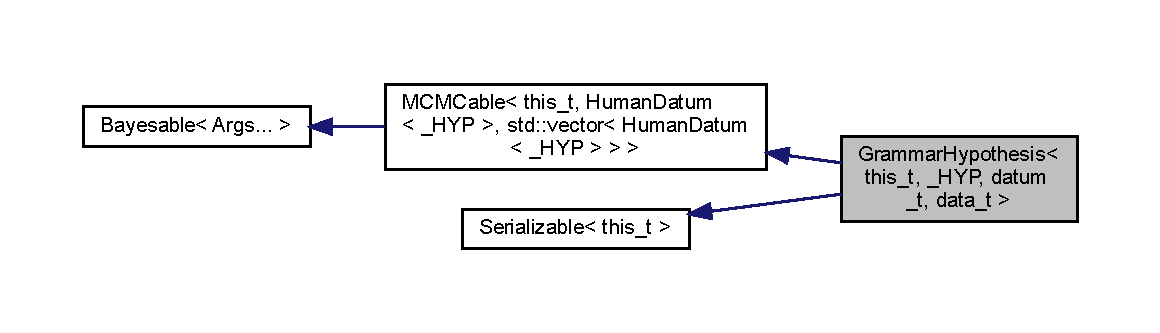
\includegraphics[width=263pt]{class_grammar_hypothesis__inherit__graph}
\end{center}
\end{figure}


Collaboration diagram for Grammar\+Hypothesis$<$ this\+\_\+t, \+\_\+\+H\+YP, datum\+\_\+t, data\+\_\+t $>$\+:
\nopagebreak
\begin{figure}[H]
\begin{center}
\leavevmode
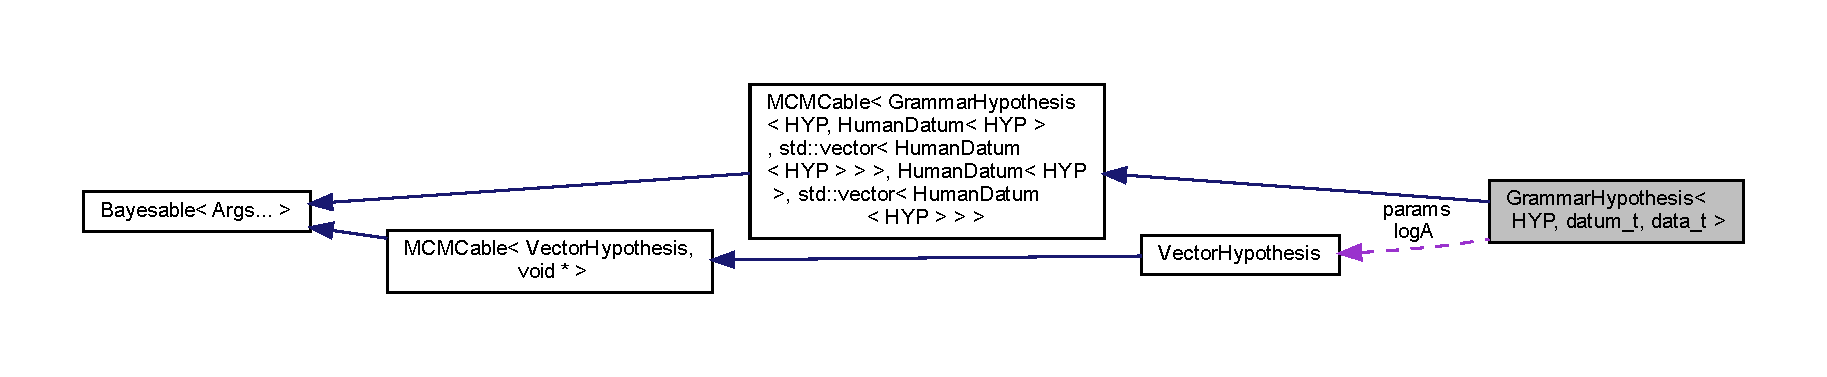
\includegraphics[width=350pt]{class_grammar_hypothesis__coll__graph}
\end{center}
\end{figure}
\doxysubsection*{Public Types}
\begin{DoxyCompactItemize}
\item 
using \mbox{\hyperlink{class_grammar_hypothesis_a28fc99df28de741179719c94ecd77699}{H\+YP}} = \+\_\+\+H\+YP
\item 
using \mbox{\hyperlink{class_grammar_hypothesis_a7c6a6c59b0ba1ca6e225079d0cb7143b}{L\+L\+\_\+t}} = std\+::unordered\+\_\+map$<$ typename datum\+\_\+t\+::data\+\_\+t $\ast$, std\+::vector$<$ Vector $>$ $>$
\item 
using \mbox{\hyperlink{class_grammar_hypothesis_aa5ecc4d2215fa50a9c2b4e7c682c7cd7}{Predict\+\_\+t}} = \mbox{\hyperlink{struct_vector2_d}{Vector2D}}$<$ std\+::vector$<$ std\+::pair$<$ typename H\+Y\+P\+::output\+\_\+t, double $>$ $>$$>$
\end{DoxyCompactItemize}
\doxysubsection*{Public Member Functions}
\begin{DoxyCompactItemize}
\item 
\mbox{\hyperlink{class_grammar_hypothesis_a83e43512aae4bfcbd0e3907a62c71132}{Grammar\+Hypothesis}} ()
\item 
\mbox{\hyperlink{class_grammar_hypothesis_af74bd80ebd8d4d1f2e16507826af5465}{Grammar\+Hypothesis}} (std\+::vector$<$ \mbox{\hyperlink{class_grammar_hypothesis_a28fc99df28de741179719c94ecd77699}{H\+YP}} $>$ \&hypotheses, const \mbox{\hyperlink{class_bayesable_aa2788c4d7718c0a824e1d28c4c98f921}{data\+\_\+t}} $\ast$human\+\_\+data)
\item 
virtual void \mbox{\hyperlink{class_grammar_hypothesis_a4073539c064e62f00e77998a04a693cb}{set\+\_\+hypotheses\+\_\+and\+\_\+data}} (std\+::vector$<$ \mbox{\hyperlink{class_grammar_hypothesis_a28fc99df28de741179719c94ecd77699}{H\+YP}} $>$ \&hypotheses, const \mbox{\hyperlink{class_bayesable_aa2788c4d7718c0a824e1d28c4c98f921}{data\+\_\+t}} \&human\+\_\+data)
\begin{DoxyCompactList}\small\item\em This is the primary function for setting hypothese and data on construction. \end{DoxyCompactList}\item 
virtual void \mbox{\hyperlink{class_grammar_hypothesis_af658323081d132788bb5bebbd07c93e8}{set\+\_\+can\+\_\+propose}} (size\+\_\+t i, bool b)
\begin{DoxyCompactList}\small\item\em Set whether I can propose to a value in logA -- this is handled by \mbox{\hyperlink{class_vector_normal_hypothesis}{Vector\+Normal\+Hypothesis}} Here, though, we warn if the value is not 1.\+0. \end{DoxyCompactList}\item 
virtual size\+\_\+t \mbox{\hyperlink{class_grammar_hypothesis_a887f646d5c07a485721d7b89bb166274}{nhypotheses}} () const
\begin{DoxyCompactList}\small\item\em A convenient function that uses C to say how many hypotheses. \end{DoxyCompactList}\item 
virtual void \mbox{\hyperlink{class_grammar_hypothesis_a6a1fadc201aa1ab1c9fe32102886ae2c}{recompute\+\_\+C}} (std\+::vector$<$ \mbox{\hyperlink{class_grammar_hypothesis_a28fc99df28de741179719c94ecd77699}{H\+YP}} $>$ \&hypotheses)
\begin{DoxyCompactList}\small\item\em Computes our matrix C\mbox{[}h,r\mbox{]} of hypotheses (rows) by counts of each grammar rule. (requires that each hypothesis use the same grammar) \end{DoxyCompactList}\item 
virtual void \mbox{\hyperlink{class_grammar_hypothesis_aa55913a4798b21974f225ec40193cfc1}{recompute\+\_\+\+LL}} (std\+::vector$<$ \mbox{\hyperlink{class_grammar_hypothesis_a28fc99df28de741179719c94ecd77699}{H\+YP}} $>$ \&hypotheses, const \mbox{\hyperlink{class_bayesable_aa2788c4d7718c0a824e1d28c4c98f921}{data\+\_\+t}} \&human\+\_\+data)
\begin{DoxyCompactList}\small\item\em Recompute LL\mbox{[}h,di\mbox{]} a hypothesis from each hypothesis and data point to a {\itshape vector} of prior responses. (We need the vector instead of just the sum to implement memory decay. \end{DoxyCompactList}\item 
virtual void \mbox{\hyperlink{class_grammar_hypothesis_a8476132b0ea0f4d0743dde525ce37ba9}{recompute\+\_\+decayed\+Likelihood}} (const \mbox{\hyperlink{class_bayesable_aa2788c4d7718c0a824e1d28c4c98f921}{data\+\_\+t}} \&human\+\_\+data)
\begin{DoxyCompactList}\small\item\em Recomputes the decayed likelihood (e.\+g. at the given decay level, the total ll for each data point. \end{DoxyCompactList}\item 
virtual void \mbox{\hyperlink{class_grammar_hypothesis_a5dc4c47ed55185ec1d1376bd0e7cdb40}{recompute\+\_\+P}} (std\+::vector$<$ \mbox{\hyperlink{class_grammar_hypothesis_a28fc99df28de741179719c94ecd77699}{H\+YP}} $>$ \&hypotheses, const \mbox{\hyperlink{class_bayesable_aa2788c4d7718c0a824e1d28c4c98f921}{data\+\_\+t}} \&human\+\_\+data)
\item 
virtual double \mbox{\hyperlink{class_grammar_hypothesis_a8ad537345ab55b581825b89c9b2cfad3}{compute\+\_\+prior}} () override
\begin{DoxyCompactList}\small\item\em Compute the prior -- defaultly not defined. \end{DoxyCompactList}\item 
virtual Matrix \mbox{\hyperlink{class_grammar_hypothesis_a2e4105060c6b5e96679fdb116591b3f1}{compute\+\_\+normalized\+\_\+posterior}} ()
\begin{DoxyCompactList}\small\item\em This returns a matrix hposter\mbox{[}h,di\mbox{]} giving the posterior on the h\textquotesingle{}th element. \end{DoxyCompactList}\item 
virtual double \mbox{\hyperlink{class_grammar_hypothesis_a769eea50d9e40668022b120b6fddfe06}{compute\+\_\+likelihood}} (const \mbox{\hyperlink{class_bayesable_aa2788c4d7718c0a824e1d28c4c98f921}{data\+\_\+t}} \&human\+\_\+data, const double breakout=-\/\mbox{\hyperlink{_numerics_8h_af9434aea82baf2f6a5d9b6f9e36db08e}{infinity}}) override
\begin{DoxyCompactList}\small\item\em This computes the likelihood of the {\itshape human data}. \end{DoxyCompactList}\item 
virtual this\+\_\+t \mbox{\hyperlink{class_grammar_hypothesis_a85c5aad5990900d4da6eca5a24deb3e6}{restart}} () const override
\item 
virtual std\+::pair$<$ this\+\_\+t, double $>$ \mbox{\hyperlink{class_grammar_hypothesis_a8e6d781ab5fa0a6656b09b607a906735}{propose}} () const override
\begin{DoxyCompactList}\small\item\em Propose to the hypothesis. The sometimes does grammar parameters and sometimes other parameters, which are all stored as Vector\+Hypotheses. It is sure to call the recompute functions when necessary. \end{DoxyCompactList}\item 
virtual Vector \mbox{\hyperlink{class_grammar_hypothesis_a3fb4235ab47fe78e77c63023c22659d7}{hypothesis\+\_\+prior}} (Matrix \&myC)
\item 
virtual bool \mbox{\hyperlink{class_grammar_hypothesis_a5af8ece466cdc1d0fc2a960ae1d63462}{operator==}} (const this\+\_\+t \&h) const override
\item 
virtual std\+::string \mbox{\hyperlink{class_grammar_hypothesis_a4f978eb7e5b7e5dc86f8a434297f8c8e}{string}} (std\+::string prefix=\char`\"{}\char`\"{}) const override
\begin{DoxyCompactList}\small\item\em This returns a string for this hypothesis. Defaulty, now, just in tidy format with all the parameters, one on each row. Note these parameters are shown after transformation (e.\+g. the prior parameters are N\+OT logged) \end{DoxyCompactList}\item 
virtual void \mbox{\hyperlink{class_grammar_hypothesis_a7b791d9da5ae86c52a42a2383c1c6bc0}{print}} (std\+::string prefix=\char`\"{}\char`\"{}) override
\begin{DoxyCompactList}\small\item\em Need to override print since it will print in a different format. \end{DoxyCompactList}\item 
virtual size\+\_\+t \mbox{\hyperlink{class_grammar_hypothesis_aeb9e858426a5ef273b87eafd8b2a5cd6}{hash}} () const override
\end{DoxyCompactItemize}
\doxysubsection*{Static Public Member Functions}
\begin{DoxyCompactItemize}
\item 
{\footnotesize template$<$typename... A$>$ }\\static this\+\_\+t \mbox{\hyperlink{class_grammar_hypothesis_a7249002c5be7aba6b88adf440600bbef}{make}} (A... a)
\end{DoxyCompactItemize}
\doxysubsection*{Public Attributes}
\begin{DoxyCompactItemize}
\item 
\mbox{\hyperlink{class_vector_normal_hypothesis}{Vector\+Normal\+Hypothesis}} \mbox{\hyperlink{class_grammar_hypothesis_a8b6e2526b457a656511dda7eb4b9e546}{logA}}
\item 
\mbox{\hyperlink{class_t_normal_variable}{T\+Normal\+Variable}}$<$+\mbox{[}$\,$\mbox{]}(float x) -\/$>$ \mbox{\hyperlink{class_grammar_hypothesis_aff7618f98de8737df436c86424cc62ed}{float}} \{ return 1.\+0/(1.\+0+expf(-\/1.\+7$\ast$x))
\item 
\mbox{\hyperlink{class_grammar_hypothesis_aad05b11be3c0249d8a22ab078d28635c}{alpha}}
\item 
\mbox{\hyperlink{class_grammar_hypothesis_a0c8f321de22c6e78d95b0e265f346892}{llt}}
\item 
\mbox{\hyperlink{class_grammar_hypothesis_a3dfa8da300156a045ac542bdd5364e0f}{pt}}
\item 
\mbox{\hyperlink{class_grammar_hypothesis_a1ff45b8e4d4e7ace3dcddb6dab5c5c58}{decay}}
\item 
H\+Y\+P\+::\+Grammar\+\_\+t $\ast$ \mbox{\hyperlink{class_grammar_hypothesis_afa17cc4569b9ac59eb3d232919a73917}{grammar}}
\item 
std\+::shared\+\_\+ptr$<$ Matrix $>$ \mbox{\hyperlink{class_grammar_hypothesis_a2b056bde1754e6e18d9a7ebfa753fc60}{C}}
\item 
std\+::shared\+\_\+ptr$<$ \mbox{\hyperlink{class_grammar_hypothesis_a7c6a6c59b0ba1ca6e225079d0cb7143b}{L\+L\+\_\+t}} $>$ \mbox{\hyperlink{class_grammar_hypothesis_a03f4757e1c6cbf99319dda821d061fe3}{LL}}
\item 
std\+::shared\+\_\+ptr$<$ \mbox{\hyperlink{class_grammar_hypothesis_aa5ecc4d2215fa50a9c2b4e7c682c7cd7}{Predict\+\_\+t}} $>$ \mbox{\hyperlink{class_grammar_hypothesis_a9b3df606fce3805c6cd1ba2dd542a73c}{P}}
\item 
std\+::shared\+\_\+ptr$<$ Matrix $>$ \mbox{\hyperlink{class_grammar_hypothesis_a9e543dfed61a4196c98135409d4b264c}{decayed\+Likelihood}}
\item 
const \mbox{\hyperlink{class_bayesable_aa2788c4d7718c0a824e1d28c4c98f921}{data\+\_\+t}} $\ast$ \mbox{\hyperlink{class_grammar_hypothesis_a91f16aecf3f2a1e9bd1386c846635dba}{which\+\_\+data}}
\end{DoxyCompactItemize}


\doxysubsection{Detailed Description}
\subsubsection*{template$<$typename this\+\_\+t, typename \+\_\+\+H\+YP, typename datum\+\_\+t = Human\+Datum$<$\+\_\+\+H\+Y\+P$>$, typename data\+\_\+t = std\+::vector$<$datum\+\_\+t$>$$>$\newline
class Grammar\+Hypothesis$<$ this\+\_\+t, \+\_\+\+H\+Y\+P, datum\+\_\+t, data\+\_\+t $>$}

\begin{DoxyAuthor}{Author}
piantado 
\end{DoxyAuthor}
\begin{DoxyDate}{Date}
02/08/20 
\end{DoxyDate}


\doxysubsection{Member Typedef Documentation}
\mbox{\Hypertarget{class_grammar_hypothesis_a28fc99df28de741179719c94ecd77699}\label{class_grammar_hypothesis_a28fc99df28de741179719c94ecd77699}} 
\index{GrammarHypothesis$<$ this\_t, \_HYP, datum\_t, data\_t $>$@{GrammarHypothesis$<$ this\_t, \_HYP, datum\_t, data\_t $>$}!HYP@{HYP}}
\index{HYP@{HYP}!GrammarHypothesis$<$ this\_t, \_HYP, datum\_t, data\_t $>$@{GrammarHypothesis$<$ this\_t, \_HYP, datum\_t, data\_t $>$}}
\doxysubsubsection{\texorpdfstring{HYP}{HYP}}
{\footnotesize\ttfamily template$<$typename this\+\_\+t , typename \+\_\+\+H\+YP , typename datum\+\_\+t  = Human\+Datum$<$\+\_\+\+H\+Y\+P$>$, typename data\+\_\+t  = std\+::vector$<$datum\+\_\+t$>$$>$ \\
using \mbox{\hyperlink{class_grammar_hypothesis}{Grammar\+Hypothesis}}$<$ this\+\_\+t, \+\_\+\+H\+YP, \mbox{\hyperlink{class_bayesable_a9f1a6c0cd7855550fa10b1a8f13a5867}{datum\+\_\+t}}, \mbox{\hyperlink{class_bayesable_aa2788c4d7718c0a824e1d28c4c98f921}{data\+\_\+t}} $>$\+::\mbox{\hyperlink{class_grammar_hypothesis_a28fc99df28de741179719c94ecd77699}{H\+YP}} =  \+\_\+\+H\+YP}

\mbox{\Hypertarget{class_grammar_hypothesis_a7c6a6c59b0ba1ca6e225079d0cb7143b}\label{class_grammar_hypothesis_a7c6a6c59b0ba1ca6e225079d0cb7143b}} 
\index{GrammarHypothesis$<$ this\_t, \_HYP, datum\_t, data\_t $>$@{GrammarHypothesis$<$ this\_t, \_HYP, datum\_t, data\_t $>$}!LL\_t@{LL\_t}}
\index{LL\_t@{LL\_t}!GrammarHypothesis$<$ this\_t, \_HYP, datum\_t, data\_t $>$@{GrammarHypothesis$<$ this\_t, \_HYP, datum\_t, data\_t $>$}}
\doxysubsubsection{\texorpdfstring{LL\_t}{LL\_t}}
{\footnotesize\ttfamily template$<$typename this\+\_\+t , typename \+\_\+\+H\+YP , typename datum\+\_\+t  = Human\+Datum$<$\+\_\+\+H\+Y\+P$>$, typename data\+\_\+t  = std\+::vector$<$datum\+\_\+t$>$$>$ \\
using \mbox{\hyperlink{class_grammar_hypothesis}{Grammar\+Hypothesis}}$<$ this\+\_\+t, \+\_\+\+H\+YP, \mbox{\hyperlink{class_bayesable_a9f1a6c0cd7855550fa10b1a8f13a5867}{datum\+\_\+t}}, \mbox{\hyperlink{class_bayesable_aa2788c4d7718c0a824e1d28c4c98f921}{data\+\_\+t}} $>$\+::\mbox{\hyperlink{class_grammar_hypothesis_a7c6a6c59b0ba1ca6e225079d0cb7143b}{L\+L\+\_\+t}} =  std\+::unordered\+\_\+map$<$typename datum\+\_\+t\+::data\+\_\+t$\ast$, std\+::vector$<$Vector$>$ $>$}

\mbox{\Hypertarget{class_grammar_hypothesis_aa5ecc4d2215fa50a9c2b4e7c682c7cd7}\label{class_grammar_hypothesis_aa5ecc4d2215fa50a9c2b4e7c682c7cd7}} 
\index{GrammarHypothesis$<$ this\_t, \_HYP, datum\_t, data\_t $>$@{GrammarHypothesis$<$ this\_t, \_HYP, datum\_t, data\_t $>$}!Predict\_t@{Predict\_t}}
\index{Predict\_t@{Predict\_t}!GrammarHypothesis$<$ this\_t, \_HYP, datum\_t, data\_t $>$@{GrammarHypothesis$<$ this\_t, \_HYP, datum\_t, data\_t $>$}}
\doxysubsubsection{\texorpdfstring{Predict\_t}{Predict\_t}}
{\footnotesize\ttfamily template$<$typename this\+\_\+t , typename \+\_\+\+H\+YP , typename datum\+\_\+t  = Human\+Datum$<$\+\_\+\+H\+Y\+P$>$, typename data\+\_\+t  = std\+::vector$<$datum\+\_\+t$>$$>$ \\
using \mbox{\hyperlink{class_grammar_hypothesis}{Grammar\+Hypothesis}}$<$ this\+\_\+t, \+\_\+\+H\+YP, \mbox{\hyperlink{class_bayesable_a9f1a6c0cd7855550fa10b1a8f13a5867}{datum\+\_\+t}}, \mbox{\hyperlink{class_bayesable_aa2788c4d7718c0a824e1d28c4c98f921}{data\+\_\+t}} $>$\+::\mbox{\hyperlink{class_grammar_hypothesis_aa5ecc4d2215fa50a9c2b4e7c682c7cd7}{Predict\+\_\+t}} =  \mbox{\hyperlink{struct_vector2_d}{Vector2D}}$<$std\+::vector$<$std\+::pair$<$typename H\+Y\+P\+::output\+\_\+t,double$>$ $>$$>$}



\doxysubsection{Constructor \& Destructor Documentation}
\mbox{\Hypertarget{class_grammar_hypothesis_a83e43512aae4bfcbd0e3907a62c71132}\label{class_grammar_hypothesis_a83e43512aae4bfcbd0e3907a62c71132}} 
\index{GrammarHypothesis$<$ this\_t, \_HYP, datum\_t, data\_t $>$@{GrammarHypothesis$<$ this\_t, \_HYP, datum\_t, data\_t $>$}!GrammarHypothesis@{GrammarHypothesis}}
\index{GrammarHypothesis@{GrammarHypothesis}!GrammarHypothesis$<$ this\_t, \_HYP, datum\_t, data\_t $>$@{GrammarHypothesis$<$ this\_t, \_HYP, datum\_t, data\_t $>$}}
\doxysubsubsection{\texorpdfstring{GrammarHypothesis()}{GrammarHypothesis()}\hspace{0.1cm}{\footnotesize\ttfamily [1/2]}}
{\footnotesize\ttfamily template$<$typename this\+\_\+t , typename \+\_\+\+H\+YP , typename datum\+\_\+t  = Human\+Datum$<$\+\_\+\+H\+Y\+P$>$, typename data\+\_\+t  = std\+::vector$<$datum\+\_\+t$>$$>$ \\
\mbox{\hyperlink{class_grammar_hypothesis}{Grammar\+Hypothesis}}$<$ this\+\_\+t, \+\_\+\+H\+YP, \mbox{\hyperlink{class_bayesable_a9f1a6c0cd7855550fa10b1a8f13a5867}{datum\+\_\+t}}, \mbox{\hyperlink{class_bayesable_aa2788c4d7718c0a824e1d28c4c98f921}{data\+\_\+t}} $>$\+::\mbox{\hyperlink{class_grammar_hypothesis}{Grammar\+Hypothesis}} (\begin{DoxyParamCaption}{ }\end{DoxyParamCaption})\hspace{0.3cm}{\ttfamily [inline]}}

\mbox{\Hypertarget{class_grammar_hypothesis_af74bd80ebd8d4d1f2e16507826af5465}\label{class_grammar_hypothesis_af74bd80ebd8d4d1f2e16507826af5465}} 
\index{GrammarHypothesis$<$ this\_t, \_HYP, datum\_t, data\_t $>$@{GrammarHypothesis$<$ this\_t, \_HYP, datum\_t, data\_t $>$}!GrammarHypothesis@{GrammarHypothesis}}
\index{GrammarHypothesis@{GrammarHypothesis}!GrammarHypothesis$<$ this\_t, \_HYP, datum\_t, data\_t $>$@{GrammarHypothesis$<$ this\_t, \_HYP, datum\_t, data\_t $>$}}
\doxysubsubsection{\texorpdfstring{GrammarHypothesis()}{GrammarHypothesis()}\hspace{0.1cm}{\footnotesize\ttfamily [2/2]}}
{\footnotesize\ttfamily template$<$typename this\+\_\+t , typename \+\_\+\+H\+YP , typename datum\+\_\+t  = Human\+Datum$<$\+\_\+\+H\+Y\+P$>$, typename data\+\_\+t  = std\+::vector$<$datum\+\_\+t$>$$>$ \\
\mbox{\hyperlink{class_grammar_hypothesis}{Grammar\+Hypothesis}}$<$ this\+\_\+t, \+\_\+\+H\+YP, \mbox{\hyperlink{class_bayesable_a9f1a6c0cd7855550fa10b1a8f13a5867}{datum\+\_\+t}}, \mbox{\hyperlink{class_bayesable_aa2788c4d7718c0a824e1d28c4c98f921}{data\+\_\+t}} $>$\+::\mbox{\hyperlink{class_grammar_hypothesis}{Grammar\+Hypothesis}} (\begin{DoxyParamCaption}\item[{std\+::vector$<$ \mbox{\hyperlink{class_grammar_hypothesis_a28fc99df28de741179719c94ecd77699}{H\+YP}} $>$ \&}]{hypotheses,  }\item[{const \mbox{\hyperlink{class_bayesable_aa2788c4d7718c0a824e1d28c4c98f921}{data\+\_\+t}} $\ast$}]{human\+\_\+data }\end{DoxyParamCaption})\hspace{0.3cm}{\ttfamily [inline]}}



\doxysubsection{Member Function Documentation}
\mbox{\Hypertarget{class_grammar_hypothesis_a769eea50d9e40668022b120b6fddfe06}\label{class_grammar_hypothesis_a769eea50d9e40668022b120b6fddfe06}} 
\index{GrammarHypothesis$<$ this\_t, \_HYP, datum\_t, data\_t $>$@{GrammarHypothesis$<$ this\_t, \_HYP, datum\_t, data\_t $>$}!compute\_likelihood@{compute\_likelihood}}
\index{compute\_likelihood@{compute\_likelihood}!GrammarHypothesis$<$ this\_t, \_HYP, datum\_t, data\_t $>$@{GrammarHypothesis$<$ this\_t, \_HYP, datum\_t, data\_t $>$}}
\doxysubsubsection{\texorpdfstring{compute\_likelihood()}{compute\_likelihood()}}
{\footnotesize\ttfamily template$<$typename this\+\_\+t , typename \+\_\+\+H\+YP , typename datum\+\_\+t  = Human\+Datum$<$\+\_\+\+H\+Y\+P$>$, typename data\+\_\+t  = std\+::vector$<$datum\+\_\+t$>$$>$ \\
virtual double \mbox{\hyperlink{class_grammar_hypothesis}{Grammar\+Hypothesis}}$<$ this\+\_\+t, \+\_\+\+H\+YP, \mbox{\hyperlink{class_bayesable_a9f1a6c0cd7855550fa10b1a8f13a5867}{datum\+\_\+t}}, \mbox{\hyperlink{class_bayesable_aa2788c4d7718c0a824e1d28c4c98f921}{data\+\_\+t}} $>$\+::compute\+\_\+likelihood (\begin{DoxyParamCaption}\item[{const \mbox{\hyperlink{class_bayesable_aa2788c4d7718c0a824e1d28c4c98f921}{data\+\_\+t}} \&}]{human\+\_\+data,  }\item[{const double}]{breakout = {\ttfamily -\/\mbox{\hyperlink{_numerics_8h_af9434aea82baf2f6a5d9b6f9e36db08e}{infinity}}} }\end{DoxyParamCaption})\hspace{0.3cm}{\ttfamily [inline]}, {\ttfamily [override]}, {\ttfamily [virtual]}}



This computes the likelihood of the {\itshape human data}. 


\begin{DoxyParams}{Parameters}
{\em data} & \\
\hline
{\em breakout} & \\
\hline
\end{DoxyParams}
\begin{DoxyReturn}{Returns}

\end{DoxyReturn}


Reimplemented from \mbox{\hyperlink{class_bayesable_a202493156cec15937bee304d807fdbdb}{Bayesable$<$ Args... $>$}}.

\mbox{\Hypertarget{class_grammar_hypothesis_a2e4105060c6b5e96679fdb116591b3f1}\label{class_grammar_hypothesis_a2e4105060c6b5e96679fdb116591b3f1}} 
\index{GrammarHypothesis$<$ this\_t, \_HYP, datum\_t, data\_t $>$@{GrammarHypothesis$<$ this\_t, \_HYP, datum\_t, data\_t $>$}!compute\_normalized\_posterior@{compute\_normalized\_posterior}}
\index{compute\_normalized\_posterior@{compute\_normalized\_posterior}!GrammarHypothesis$<$ this\_t, \_HYP, datum\_t, data\_t $>$@{GrammarHypothesis$<$ this\_t, \_HYP, datum\_t, data\_t $>$}}
\doxysubsubsection{\texorpdfstring{compute\_normalized\_posterior()}{compute\_normalized\_posterior()}}
{\footnotesize\ttfamily template$<$typename this\+\_\+t , typename \+\_\+\+H\+YP , typename datum\+\_\+t  = Human\+Datum$<$\+\_\+\+H\+Y\+P$>$, typename data\+\_\+t  = std\+::vector$<$datum\+\_\+t$>$$>$ \\
virtual Matrix \mbox{\hyperlink{class_grammar_hypothesis}{Grammar\+Hypothesis}}$<$ this\+\_\+t, \+\_\+\+H\+YP, \mbox{\hyperlink{class_bayesable_a9f1a6c0cd7855550fa10b1a8f13a5867}{datum\+\_\+t}}, \mbox{\hyperlink{class_bayesable_aa2788c4d7718c0a824e1d28c4c98f921}{data\+\_\+t}} $>$\+::compute\+\_\+normalized\+\_\+posterior (\begin{DoxyParamCaption}{ }\end{DoxyParamCaption})\hspace{0.3cm}{\ttfamily [inline]}, {\ttfamily [virtual]}}



This returns a matrix hposter\mbox{[}h,di\mbox{]} giving the posterior on the h\textquotesingle{}th element. 

\begin{DoxyReturn}{Returns}

\end{DoxyReturn}
\mbox{\Hypertarget{class_grammar_hypothesis_a8ad537345ab55b581825b89c9b2cfad3}\label{class_grammar_hypothesis_a8ad537345ab55b581825b89c9b2cfad3}} 
\index{GrammarHypothesis$<$ this\_t, \_HYP, datum\_t, data\_t $>$@{GrammarHypothesis$<$ this\_t, \_HYP, datum\_t, data\_t $>$}!compute\_prior@{compute\_prior}}
\index{compute\_prior@{compute\_prior}!GrammarHypothesis$<$ this\_t, \_HYP, datum\_t, data\_t $>$@{GrammarHypothesis$<$ this\_t, \_HYP, datum\_t, data\_t $>$}}
\doxysubsubsection{\texorpdfstring{compute\_prior()}{compute\_prior()}}
{\footnotesize\ttfamily template$<$typename this\+\_\+t , typename \+\_\+\+H\+YP , typename datum\+\_\+t  = Human\+Datum$<$\+\_\+\+H\+Y\+P$>$, typename data\+\_\+t  = std\+::vector$<$datum\+\_\+t$>$$>$ \\
virtual double \mbox{\hyperlink{class_grammar_hypothesis}{Grammar\+Hypothesis}}$<$ this\+\_\+t, \+\_\+\+H\+YP, \mbox{\hyperlink{class_bayesable_a9f1a6c0cd7855550fa10b1a8f13a5867}{datum\+\_\+t}}, \mbox{\hyperlink{class_bayesable_aa2788c4d7718c0a824e1d28c4c98f921}{data\+\_\+t}} $>$\+::compute\+\_\+prior (\begin{DoxyParamCaption}{ }\end{DoxyParamCaption})\hspace{0.3cm}{\ttfamily [inline]}, {\ttfamily [override]}, {\ttfamily [virtual]}}



Compute the prior -- defaultly not defined. 



Implements \mbox{\hyperlink{class_bayesable_a1b057a17212ced123545133e2297c01b}{Bayesable$<$ Args... $>$}}.

\mbox{\Hypertarget{class_grammar_hypothesis_aeb9e858426a5ef273b87eafd8b2a5cd6}\label{class_grammar_hypothesis_aeb9e858426a5ef273b87eafd8b2a5cd6}} 
\index{GrammarHypothesis$<$ this\_t, \_HYP, datum\_t, data\_t $>$@{GrammarHypothesis$<$ this\_t, \_HYP, datum\_t, data\_t $>$}!hash@{hash}}
\index{hash@{hash}!GrammarHypothesis$<$ this\_t, \_HYP, datum\_t, data\_t $>$@{GrammarHypothesis$<$ this\_t, \_HYP, datum\_t, data\_t $>$}}
\doxysubsubsection{\texorpdfstring{hash()}{hash()}}
{\footnotesize\ttfamily template$<$typename this\+\_\+t , typename \+\_\+\+H\+YP , typename datum\+\_\+t  = Human\+Datum$<$\+\_\+\+H\+Y\+P$>$, typename data\+\_\+t  = std\+::vector$<$datum\+\_\+t$>$$>$ \\
virtual size\+\_\+t \mbox{\hyperlink{class_grammar_hypothesis}{Grammar\+Hypothesis}}$<$ this\+\_\+t, \+\_\+\+H\+YP, \mbox{\hyperlink{class_bayesable_a9f1a6c0cd7855550fa10b1a8f13a5867}{datum\+\_\+t}}, \mbox{\hyperlink{class_bayesable_aa2788c4d7718c0a824e1d28c4c98f921}{data\+\_\+t}} $>$\+::hash (\begin{DoxyParamCaption}{ }\end{DoxyParamCaption}) const\hspace{0.3cm}{\ttfamily [inline]}, {\ttfamily [override]}, {\ttfamily [virtual]}}

\mbox{\Hypertarget{class_grammar_hypothesis_a3fb4235ab47fe78e77c63023c22659d7}\label{class_grammar_hypothesis_a3fb4235ab47fe78e77c63023c22659d7}} 
\index{GrammarHypothesis$<$ this\_t, \_HYP, datum\_t, data\_t $>$@{GrammarHypothesis$<$ this\_t, \_HYP, datum\_t, data\_t $>$}!hypothesis\_prior@{hypothesis\_prior}}
\index{hypothesis\_prior@{hypothesis\_prior}!GrammarHypothesis$<$ this\_t, \_HYP, datum\_t, data\_t $>$@{GrammarHypothesis$<$ this\_t, \_HYP, datum\_t, data\_t $>$}}
\doxysubsubsection{\texorpdfstring{hypothesis\_prior()}{hypothesis\_prior()}}
{\footnotesize\ttfamily template$<$typename this\+\_\+t , typename \+\_\+\+H\+YP , typename datum\+\_\+t  = Human\+Datum$<$\+\_\+\+H\+Y\+P$>$, typename data\+\_\+t  = std\+::vector$<$datum\+\_\+t$>$$>$ \\
virtual Vector \mbox{\hyperlink{class_grammar_hypothesis}{Grammar\+Hypothesis}}$<$ this\+\_\+t, \+\_\+\+H\+YP, \mbox{\hyperlink{class_bayesable_a9f1a6c0cd7855550fa10b1a8f13a5867}{datum\+\_\+t}}, \mbox{\hyperlink{class_bayesable_aa2788c4d7718c0a824e1d28c4c98f921}{data\+\_\+t}} $>$\+::hypothesis\+\_\+prior (\begin{DoxyParamCaption}\item[{Matrix \&}]{myC }\end{DoxyParamCaption})\hspace{0.3cm}{\ttfamily [inline]}, {\ttfamily [virtual]}}


\begin{DoxyParams}{Parameters}
{\em C} & \\
\hline
\end{DoxyParams}
\begin{DoxyReturn}{Returns}

\end{DoxyReturn}
\mbox{\Hypertarget{class_grammar_hypothesis_a7249002c5be7aba6b88adf440600bbef}\label{class_grammar_hypothesis_a7249002c5be7aba6b88adf440600bbef}} 
\index{GrammarHypothesis$<$ this\_t, \_HYP, datum\_t, data\_t $>$@{GrammarHypothesis$<$ this\_t, \_HYP, datum\_t, data\_t $>$}!make@{make}}
\index{make@{make}!GrammarHypothesis$<$ this\_t, \_HYP, datum\_t, data\_t $>$@{GrammarHypothesis$<$ this\_t, \_HYP, datum\_t, data\_t $>$}}
\doxysubsubsection{\texorpdfstring{make()}{make()}}
{\footnotesize\ttfamily template$<$typename this\+\_\+t , typename \+\_\+\+H\+YP , typename datum\+\_\+t  = Human\+Datum$<$\+\_\+\+H\+Y\+P$>$, typename data\+\_\+t  = std\+::vector$<$datum\+\_\+t$>$$>$ \\
template$<$typename... A$>$ \\
static this\+\_\+t \mbox{\hyperlink{class_grammar_hypothesis}{Grammar\+Hypothesis}}$<$ this\+\_\+t, \+\_\+\+H\+YP, \mbox{\hyperlink{class_bayesable_a9f1a6c0cd7855550fa10b1a8f13a5867}{datum\+\_\+t}}, \mbox{\hyperlink{class_bayesable_aa2788c4d7718c0a824e1d28c4c98f921}{data\+\_\+t}} $>$\+::make (\begin{DoxyParamCaption}\item[{A...}]{a }\end{DoxyParamCaption})\hspace{0.3cm}{\ttfamily [inline]}, {\ttfamily [static]}}

\mbox{\Hypertarget{class_grammar_hypothesis_a887f646d5c07a485721d7b89bb166274}\label{class_grammar_hypothesis_a887f646d5c07a485721d7b89bb166274}} 
\index{GrammarHypothesis$<$ this\_t, \_HYP, datum\_t, data\_t $>$@{GrammarHypothesis$<$ this\_t, \_HYP, datum\_t, data\_t $>$}!nhypotheses@{nhypotheses}}
\index{nhypotheses@{nhypotheses}!GrammarHypothesis$<$ this\_t, \_HYP, datum\_t, data\_t $>$@{GrammarHypothesis$<$ this\_t, \_HYP, datum\_t, data\_t $>$}}
\doxysubsubsection{\texorpdfstring{nhypotheses()}{nhypotheses()}}
{\footnotesize\ttfamily template$<$typename this\+\_\+t , typename \+\_\+\+H\+YP , typename datum\+\_\+t  = Human\+Datum$<$\+\_\+\+H\+Y\+P$>$, typename data\+\_\+t  = std\+::vector$<$datum\+\_\+t$>$$>$ \\
virtual size\+\_\+t \mbox{\hyperlink{class_grammar_hypothesis}{Grammar\+Hypothesis}}$<$ this\+\_\+t, \+\_\+\+H\+YP, \mbox{\hyperlink{class_bayesable_a9f1a6c0cd7855550fa10b1a8f13a5867}{datum\+\_\+t}}, \mbox{\hyperlink{class_bayesable_aa2788c4d7718c0a824e1d28c4c98f921}{data\+\_\+t}} $>$\+::nhypotheses (\begin{DoxyParamCaption}{ }\end{DoxyParamCaption}) const\hspace{0.3cm}{\ttfamily [inline]}, {\ttfamily [virtual]}}



A convenient function that uses C to say how many hypotheses. 

\begin{DoxyReturn}{Returns}

\end{DoxyReturn}
\mbox{\Hypertarget{class_grammar_hypothesis_a5af8ece466cdc1d0fc2a960ae1d63462}\label{class_grammar_hypothesis_a5af8ece466cdc1d0fc2a960ae1d63462}} 
\index{GrammarHypothesis$<$ this\_t, \_HYP, datum\_t, data\_t $>$@{GrammarHypothesis$<$ this\_t, \_HYP, datum\_t, data\_t $>$}!operator==@{operator==}}
\index{operator==@{operator==}!GrammarHypothesis$<$ this\_t, \_HYP, datum\_t, data\_t $>$@{GrammarHypothesis$<$ this\_t, \_HYP, datum\_t, data\_t $>$}}
\doxysubsubsection{\texorpdfstring{operator==()}{operator==()}}
{\footnotesize\ttfamily template$<$typename this\+\_\+t , typename \+\_\+\+H\+YP , typename datum\+\_\+t  = Human\+Datum$<$\+\_\+\+H\+Y\+P$>$, typename data\+\_\+t  = std\+::vector$<$datum\+\_\+t$>$$>$ \\
virtual bool \mbox{\hyperlink{class_grammar_hypothesis}{Grammar\+Hypothesis}}$<$ this\+\_\+t, \+\_\+\+H\+YP, \mbox{\hyperlink{class_bayesable_a9f1a6c0cd7855550fa10b1a8f13a5867}{datum\+\_\+t}}, \mbox{\hyperlink{class_bayesable_aa2788c4d7718c0a824e1d28c4c98f921}{data\+\_\+t}} $>$\+::operator== (\begin{DoxyParamCaption}\item[{const this\+\_\+t \&}]{h }\end{DoxyParamCaption}) const\hspace{0.3cm}{\ttfamily [inline]}, {\ttfamily [override]}, {\ttfamily [virtual]}}



Implements \mbox{\hyperlink{class_m_c_m_cable_a7b35c04d3d1326b930cfc69dfe0bd207}{M\+C\+M\+Cable$<$ this\+\_\+t, Human\+Datum$<$ \+\_\+\+H\+Y\+P $>$, std\+::vector$<$ Human\+Datum$<$ \+\_\+\+H\+Y\+P $>$ $>$ $>$}}.

\mbox{\Hypertarget{class_grammar_hypothesis_a7b791d9da5ae86c52a42a2383c1c6bc0}\label{class_grammar_hypothesis_a7b791d9da5ae86c52a42a2383c1c6bc0}} 
\index{GrammarHypothesis$<$ this\_t, \_HYP, datum\_t, data\_t $>$@{GrammarHypothesis$<$ this\_t, \_HYP, datum\_t, data\_t $>$}!print@{print}}
\index{print@{print}!GrammarHypothesis$<$ this\_t, \_HYP, datum\_t, data\_t $>$@{GrammarHypothesis$<$ this\_t, \_HYP, datum\_t, data\_t $>$}}
\doxysubsubsection{\texorpdfstring{print()}{print()}}
{\footnotesize\ttfamily template$<$typename this\+\_\+t , typename \+\_\+\+H\+YP , typename datum\+\_\+t  = Human\+Datum$<$\+\_\+\+H\+Y\+P$>$, typename data\+\_\+t  = std\+::vector$<$datum\+\_\+t$>$$>$ \\
virtual void \mbox{\hyperlink{class_grammar_hypothesis}{Grammar\+Hypothesis}}$<$ this\+\_\+t, \+\_\+\+H\+YP, \mbox{\hyperlink{class_bayesable_a9f1a6c0cd7855550fa10b1a8f13a5867}{datum\+\_\+t}}, \mbox{\hyperlink{class_bayesable_aa2788c4d7718c0a824e1d28c4c98f921}{data\+\_\+t}} $>$\+::print (\begin{DoxyParamCaption}\item[{std\+::string}]{prefix = {\ttfamily \char`\"{}\char`\"{}} }\end{DoxyParamCaption})\hspace{0.3cm}{\ttfamily [inline]}, {\ttfamily [override]}, {\ttfamily [virtual]}}



Need to override print since it will print in a different format. 

\begin{DoxyReturn}{Returns}

\end{DoxyReturn}


Reimplemented from \mbox{\hyperlink{class_bayesable_a87d5d9481d6a72b017e44b175071fa5e}{Bayesable$<$ Args... $>$}}.

\mbox{\Hypertarget{class_grammar_hypothesis_a8e6d781ab5fa0a6656b09b607a906735}\label{class_grammar_hypothesis_a8e6d781ab5fa0a6656b09b607a906735}} 
\index{GrammarHypothesis$<$ this\_t, \_HYP, datum\_t, data\_t $>$@{GrammarHypothesis$<$ this\_t, \_HYP, datum\_t, data\_t $>$}!propose@{propose}}
\index{propose@{propose}!GrammarHypothesis$<$ this\_t, \_HYP, datum\_t, data\_t $>$@{GrammarHypothesis$<$ this\_t, \_HYP, datum\_t, data\_t $>$}}
\doxysubsubsection{\texorpdfstring{propose()}{propose()}}
{\footnotesize\ttfamily template$<$typename this\+\_\+t , typename \+\_\+\+H\+YP , typename datum\+\_\+t  = Human\+Datum$<$\+\_\+\+H\+Y\+P$>$, typename data\+\_\+t  = std\+::vector$<$datum\+\_\+t$>$$>$ \\
virtual std\+::pair$<$this\+\_\+t,double$>$ \mbox{\hyperlink{class_grammar_hypothesis}{Grammar\+Hypothesis}}$<$ this\+\_\+t, \+\_\+\+H\+YP, \mbox{\hyperlink{class_bayesable_a9f1a6c0cd7855550fa10b1a8f13a5867}{datum\+\_\+t}}, \mbox{\hyperlink{class_bayesable_aa2788c4d7718c0a824e1d28c4c98f921}{data\+\_\+t}} $>$\+::propose (\begin{DoxyParamCaption}{ }\end{DoxyParamCaption}) const\hspace{0.3cm}{\ttfamily [inline]}, {\ttfamily [override]}, {\ttfamily [virtual]}}



Propose to the hypothesis. The sometimes does grammar parameters and sometimes other parameters, which are all stored as Vector\+Hypotheses. It is sure to call the recompute functions when necessary. 


\begin{DoxyParams}{Parameters}
{\em data} & \\
\hline
{\em breakout} & \\
\hline
\end{DoxyParams}
\begin{DoxyReturn}{Returns}

\end{DoxyReturn}
\mbox{\Hypertarget{class_grammar_hypothesis_a6a1fadc201aa1ab1c9fe32102886ae2c}\label{class_grammar_hypothesis_a6a1fadc201aa1ab1c9fe32102886ae2c}} 
\index{GrammarHypothesis$<$ this\_t, \_HYP, datum\_t, data\_t $>$@{GrammarHypothesis$<$ this\_t, \_HYP, datum\_t, data\_t $>$}!recompute\_C@{recompute\_C}}
\index{recompute\_C@{recompute\_C}!GrammarHypothesis$<$ this\_t, \_HYP, datum\_t, data\_t $>$@{GrammarHypothesis$<$ this\_t, \_HYP, datum\_t, data\_t $>$}}
\doxysubsubsection{\texorpdfstring{recompute\_C()}{recompute\_C()}}
{\footnotesize\ttfamily template$<$typename this\+\_\+t , typename \+\_\+\+H\+YP , typename datum\+\_\+t  = Human\+Datum$<$\+\_\+\+H\+Y\+P$>$, typename data\+\_\+t  = std\+::vector$<$datum\+\_\+t$>$$>$ \\
virtual void \mbox{\hyperlink{class_grammar_hypothesis}{Grammar\+Hypothesis}}$<$ this\+\_\+t, \+\_\+\+H\+YP, \mbox{\hyperlink{class_bayesable_a9f1a6c0cd7855550fa10b1a8f13a5867}{datum\+\_\+t}}, \mbox{\hyperlink{class_bayesable_aa2788c4d7718c0a824e1d28c4c98f921}{data\+\_\+t}} $>$\+::recompute\+\_\+C (\begin{DoxyParamCaption}\item[{std\+::vector$<$ \mbox{\hyperlink{class_grammar_hypothesis_a28fc99df28de741179719c94ecd77699}{H\+YP}} $>$ \&}]{hypotheses }\end{DoxyParamCaption})\hspace{0.3cm}{\ttfamily [inline]}, {\ttfamily [virtual]}}



Computes our matrix C\mbox{[}h,r\mbox{]} of hypotheses (rows) by counts of each grammar rule. (requires that each hypothesis use the same grammar) 


\begin{DoxyParams}{Parameters}
{\em hypotheses} & \\
\hline
\end{DoxyParams}
\mbox{\Hypertarget{class_grammar_hypothesis_a8476132b0ea0f4d0743dde525ce37ba9}\label{class_grammar_hypothesis_a8476132b0ea0f4d0743dde525ce37ba9}} 
\index{GrammarHypothesis$<$ this\_t, \_HYP, datum\_t, data\_t $>$@{GrammarHypothesis$<$ this\_t, \_HYP, datum\_t, data\_t $>$}!recompute\_decayedLikelihood@{recompute\_decayedLikelihood}}
\index{recompute\_decayedLikelihood@{recompute\_decayedLikelihood}!GrammarHypothesis$<$ this\_t, \_HYP, datum\_t, data\_t $>$@{GrammarHypothesis$<$ this\_t, \_HYP, datum\_t, data\_t $>$}}
\doxysubsubsection{\texorpdfstring{recompute\_decayedLikelihood()}{recompute\_decayedLikelihood()}}
{\footnotesize\ttfamily template$<$typename this\+\_\+t , typename \+\_\+\+H\+YP , typename datum\+\_\+t  = Human\+Datum$<$\+\_\+\+H\+Y\+P$>$, typename data\+\_\+t  = std\+::vector$<$datum\+\_\+t$>$$>$ \\
virtual void \mbox{\hyperlink{class_grammar_hypothesis}{Grammar\+Hypothesis}}$<$ this\+\_\+t, \+\_\+\+H\+YP, \mbox{\hyperlink{class_bayesable_a9f1a6c0cd7855550fa10b1a8f13a5867}{datum\+\_\+t}}, \mbox{\hyperlink{class_bayesable_aa2788c4d7718c0a824e1d28c4c98f921}{data\+\_\+t}} $>$\+::recompute\+\_\+decayed\+Likelihood (\begin{DoxyParamCaption}\item[{const \mbox{\hyperlink{class_bayesable_aa2788c4d7718c0a824e1d28c4c98f921}{data\+\_\+t}} \&}]{human\+\_\+data }\end{DoxyParamCaption})\hspace{0.3cm}{\ttfamily [inline]}, {\ttfamily [virtual]}}



Recomputes the decayed likelihood (e.\+g. at the given decay level, the total ll for each data point. 


\begin{DoxyParams}{Parameters}
{\em hypotheses} & \\
\hline
{\em human\+\_\+data} & \\
\hline
\end{DoxyParams}
\begin{DoxyReturn}{Returns}

\end{DoxyReturn}
\mbox{\Hypertarget{class_grammar_hypothesis_aa55913a4798b21974f225ec40193cfc1}\label{class_grammar_hypothesis_aa55913a4798b21974f225ec40193cfc1}} 
\index{GrammarHypothesis$<$ this\_t, \_HYP, datum\_t, data\_t $>$@{GrammarHypothesis$<$ this\_t, \_HYP, datum\_t, data\_t $>$}!recompute\_LL@{recompute\_LL}}
\index{recompute\_LL@{recompute\_LL}!GrammarHypothesis$<$ this\_t, \_HYP, datum\_t, data\_t $>$@{GrammarHypothesis$<$ this\_t, \_HYP, datum\_t, data\_t $>$}}
\doxysubsubsection{\texorpdfstring{recompute\_LL()}{recompute\_LL()}}
{\footnotesize\ttfamily template$<$typename this\+\_\+t , typename \+\_\+\+H\+YP , typename datum\+\_\+t  = Human\+Datum$<$\+\_\+\+H\+Y\+P$>$, typename data\+\_\+t  = std\+::vector$<$datum\+\_\+t$>$$>$ \\
virtual void \mbox{\hyperlink{class_grammar_hypothesis}{Grammar\+Hypothesis}}$<$ this\+\_\+t, \+\_\+\+H\+YP, \mbox{\hyperlink{class_bayesable_a9f1a6c0cd7855550fa10b1a8f13a5867}{datum\+\_\+t}}, \mbox{\hyperlink{class_bayesable_aa2788c4d7718c0a824e1d28c4c98f921}{data\+\_\+t}} $>$\+::recompute\+\_\+\+LL (\begin{DoxyParamCaption}\item[{std\+::vector$<$ \mbox{\hyperlink{class_grammar_hypothesis_a28fc99df28de741179719c94ecd77699}{H\+YP}} $>$ \&}]{hypotheses,  }\item[{const \mbox{\hyperlink{class_bayesable_aa2788c4d7718c0a824e1d28c4c98f921}{data\+\_\+t}} \&}]{human\+\_\+data }\end{DoxyParamCaption})\hspace{0.3cm}{\ttfamily [inline]}, {\ttfamily [virtual]}}



Recompute LL\mbox{[}h,di\mbox{]} a hypothesis from each hypothesis and data point to a {\itshape vector} of prior responses. (We need the vector instead of just the sum to implement memory decay. 


\begin{DoxyParams}{Parameters}
{\em hypotheses} & \\
\hline
{\em human\+\_\+data} & \\
\hline
\end{DoxyParams}
\begin{DoxyReturn}{Returns}

\end{DoxyReturn}
\mbox{\Hypertarget{class_grammar_hypothesis_a5dc4c47ed55185ec1d1376bd0e7cdb40}\label{class_grammar_hypothesis_a5dc4c47ed55185ec1d1376bd0e7cdb40}} 
\index{GrammarHypothesis$<$ this\_t, \_HYP, datum\_t, data\_t $>$@{GrammarHypothesis$<$ this\_t, \_HYP, datum\_t, data\_t $>$}!recompute\_P@{recompute\_P}}
\index{recompute\_P@{recompute\_P}!GrammarHypothesis$<$ this\_t, \_HYP, datum\_t, data\_t $>$@{GrammarHypothesis$<$ this\_t, \_HYP, datum\_t, data\_t $>$}}
\doxysubsubsection{\texorpdfstring{recompute\_P()}{recompute\_P()}}
{\footnotesize\ttfamily template$<$typename this\+\_\+t , typename \+\_\+\+H\+YP , typename datum\+\_\+t  = Human\+Datum$<$\+\_\+\+H\+Y\+P$>$, typename data\+\_\+t  = std\+::vector$<$datum\+\_\+t$>$$>$ \\
virtual void \mbox{\hyperlink{class_grammar_hypothesis}{Grammar\+Hypothesis}}$<$ this\+\_\+t, \+\_\+\+H\+YP, \mbox{\hyperlink{class_bayesable_a9f1a6c0cd7855550fa10b1a8f13a5867}{datum\+\_\+t}}, \mbox{\hyperlink{class_bayesable_aa2788c4d7718c0a824e1d28c4c98f921}{data\+\_\+t}} $>$\+::recompute\+\_\+P (\begin{DoxyParamCaption}\item[{std\+::vector$<$ \mbox{\hyperlink{class_grammar_hypothesis_a28fc99df28de741179719c94ecd77699}{H\+YP}} $>$ \&}]{hypotheses,  }\item[{const \mbox{\hyperlink{class_bayesable_aa2788c4d7718c0a824e1d28c4c98f921}{data\+\_\+t}} \&}]{human\+\_\+data }\end{DoxyParamCaption})\hspace{0.3cm}{\ttfamily [inline]}, {\ttfamily [virtual]}}


\begin{DoxyParams}{Parameters}
{\em hypotheses} & \\
\hline
{\em human\+\_\+data} & \\
\hline
\end{DoxyParams}
\begin{DoxyReturn}{Returns}

\end{DoxyReturn}
\mbox{\Hypertarget{class_grammar_hypothesis_a85c5aad5990900d4da6eca5a24deb3e6}\label{class_grammar_hypothesis_a85c5aad5990900d4da6eca5a24deb3e6}} 
\index{GrammarHypothesis$<$ this\_t, \_HYP, datum\_t, data\_t $>$@{GrammarHypothesis$<$ this\_t, \_HYP, datum\_t, data\_t $>$}!restart@{restart}}
\index{restart@{restart}!GrammarHypothesis$<$ this\_t, \_HYP, datum\_t, data\_t $>$@{GrammarHypothesis$<$ this\_t, \_HYP, datum\_t, data\_t $>$}}
\doxysubsubsection{\texorpdfstring{restart()}{restart()}}
{\footnotesize\ttfamily template$<$typename this\+\_\+t , typename \+\_\+\+H\+YP , typename datum\+\_\+t  = Human\+Datum$<$\+\_\+\+H\+Y\+P$>$, typename data\+\_\+t  = std\+::vector$<$datum\+\_\+t$>$$>$ \\
virtual this\+\_\+t \mbox{\hyperlink{class_grammar_hypothesis}{Grammar\+Hypothesis}}$<$ this\+\_\+t, \+\_\+\+H\+YP, \mbox{\hyperlink{class_bayesable_a9f1a6c0cd7855550fa10b1a8f13a5867}{datum\+\_\+t}}, \mbox{\hyperlink{class_bayesable_aa2788c4d7718c0a824e1d28c4c98f921}{data\+\_\+t}} $>$\+::restart (\begin{DoxyParamCaption}{ }\end{DoxyParamCaption}) const\hspace{0.3cm}{\ttfamily [inline]}, {\ttfamily [override]}, {\ttfamily [virtual]}}

\mbox{\Hypertarget{class_grammar_hypothesis_af658323081d132788bb5bebbd07c93e8}\label{class_grammar_hypothesis_af658323081d132788bb5bebbd07c93e8}} 
\index{GrammarHypothesis$<$ this\_t, \_HYP, datum\_t, data\_t $>$@{GrammarHypothesis$<$ this\_t, \_HYP, datum\_t, data\_t $>$}!set\_can\_propose@{set\_can\_propose}}
\index{set\_can\_propose@{set\_can\_propose}!GrammarHypothesis$<$ this\_t, \_HYP, datum\_t, data\_t $>$@{GrammarHypothesis$<$ this\_t, \_HYP, datum\_t, data\_t $>$}}
\doxysubsubsection{\texorpdfstring{set\_can\_propose()}{set\_can\_propose()}}
{\footnotesize\ttfamily template$<$typename this\+\_\+t , typename \+\_\+\+H\+YP , typename datum\+\_\+t  = Human\+Datum$<$\+\_\+\+H\+Y\+P$>$, typename data\+\_\+t  = std\+::vector$<$datum\+\_\+t$>$$>$ \\
virtual void \mbox{\hyperlink{class_grammar_hypothesis}{Grammar\+Hypothesis}}$<$ this\+\_\+t, \+\_\+\+H\+YP, \mbox{\hyperlink{class_bayesable_a9f1a6c0cd7855550fa10b1a8f13a5867}{datum\+\_\+t}}, \mbox{\hyperlink{class_bayesable_aa2788c4d7718c0a824e1d28c4c98f921}{data\+\_\+t}} $>$\+::set\+\_\+can\+\_\+propose (\begin{DoxyParamCaption}\item[{size\+\_\+t}]{i,  }\item[{bool}]{b }\end{DoxyParamCaption})\hspace{0.3cm}{\ttfamily [inline]}, {\ttfamily [virtual]}}



Set whether I can propose to a value in logA -- this is handled by \mbox{\hyperlink{class_vector_normal_hypothesis}{Vector\+Normal\+Hypothesis}} Here, though, we warn if the value is not 1.\+0. 


\begin{DoxyParams}{Parameters}
{\em i} & \\
\hline
{\em b} & \\
\hline
\end{DoxyParams}
\mbox{\Hypertarget{class_grammar_hypothesis_a4073539c064e62f00e77998a04a693cb}\label{class_grammar_hypothesis_a4073539c064e62f00e77998a04a693cb}} 
\index{GrammarHypothesis$<$ this\_t, \_HYP, datum\_t, data\_t $>$@{GrammarHypothesis$<$ this\_t, \_HYP, datum\_t, data\_t $>$}!set\_hypotheses\_and\_data@{set\_hypotheses\_and\_data}}
\index{set\_hypotheses\_and\_data@{set\_hypotheses\_and\_data}!GrammarHypothesis$<$ this\_t, \_HYP, datum\_t, data\_t $>$@{GrammarHypothesis$<$ this\_t, \_HYP, datum\_t, data\_t $>$}}
\doxysubsubsection{\texorpdfstring{set\_hypotheses\_and\_data()}{set\_hypotheses\_and\_data()}}
{\footnotesize\ttfamily template$<$typename this\+\_\+t , typename \+\_\+\+H\+YP , typename datum\+\_\+t  = Human\+Datum$<$\+\_\+\+H\+Y\+P$>$, typename data\+\_\+t  = std\+::vector$<$datum\+\_\+t$>$$>$ \\
virtual void \mbox{\hyperlink{class_grammar_hypothesis}{Grammar\+Hypothesis}}$<$ this\+\_\+t, \+\_\+\+H\+YP, \mbox{\hyperlink{class_bayesable_a9f1a6c0cd7855550fa10b1a8f13a5867}{datum\+\_\+t}}, \mbox{\hyperlink{class_bayesable_aa2788c4d7718c0a824e1d28c4c98f921}{data\+\_\+t}} $>$\+::set\+\_\+hypotheses\+\_\+and\+\_\+data (\begin{DoxyParamCaption}\item[{std\+::vector$<$ \mbox{\hyperlink{class_grammar_hypothesis_a28fc99df28de741179719c94ecd77699}{H\+YP}} $>$ \&}]{hypotheses,  }\item[{const \mbox{\hyperlink{class_bayesable_aa2788c4d7718c0a824e1d28c4c98f921}{data\+\_\+t}} \&}]{human\+\_\+data }\end{DoxyParamCaption})\hspace{0.3cm}{\ttfamily [inline]}, {\ttfamily [virtual]}}



This is the primary function for setting hypothese and data on construction. 


\begin{DoxyParams}{Parameters}
{\em hypotheses} & \\
\hline
{\em human\+\_\+data} & \\
\hline
\end{DoxyParams}
\mbox{\Hypertarget{class_grammar_hypothesis_a4f978eb7e5b7e5dc86f8a434297f8c8e}\label{class_grammar_hypothesis_a4f978eb7e5b7e5dc86f8a434297f8c8e}} 
\index{GrammarHypothesis$<$ this\_t, \_HYP, datum\_t, data\_t $>$@{GrammarHypothesis$<$ this\_t, \_HYP, datum\_t, data\_t $>$}!string@{string}}
\index{string@{string}!GrammarHypothesis$<$ this\_t, \_HYP, datum\_t, data\_t $>$@{GrammarHypothesis$<$ this\_t, \_HYP, datum\_t, data\_t $>$}}
\doxysubsubsection{\texorpdfstring{string()}{string()}}
{\footnotesize\ttfamily template$<$typename this\+\_\+t , typename \+\_\+\+H\+YP , typename datum\+\_\+t  = Human\+Datum$<$\+\_\+\+H\+Y\+P$>$, typename data\+\_\+t  = std\+::vector$<$datum\+\_\+t$>$$>$ \\
virtual std\+::string \mbox{\hyperlink{class_grammar_hypothesis}{Grammar\+Hypothesis}}$<$ this\+\_\+t, \+\_\+\+H\+YP, \mbox{\hyperlink{class_bayesable_a9f1a6c0cd7855550fa10b1a8f13a5867}{datum\+\_\+t}}, \mbox{\hyperlink{class_bayesable_aa2788c4d7718c0a824e1d28c4c98f921}{data\+\_\+t}} $>$\+::string (\begin{DoxyParamCaption}\item[{std\+::string}]{prefix = {\ttfamily \char`\"{}\char`\"{}} }\end{DoxyParamCaption}) const\hspace{0.3cm}{\ttfamily [inline]}, {\ttfamily [override]}, {\ttfamily [virtual]}}



This returns a string for this hypothesis. Defaulty, now, just in tidy format with all the parameters, one on each row. Note these parameters are shown after transformation (e.\+g. the prior parameters are N\+OT logged) 

\begin{DoxyReturn}{Returns}

\end{DoxyReturn}


Implements \mbox{\hyperlink{class_bayesable_ab6944b4bfe5620c96048287a51d019c1}{Bayesable$<$ Args... $>$}}.



\doxysubsection{Member Data Documentation}
\mbox{\Hypertarget{class_grammar_hypothesis_aad05b11be3c0249d8a22ab078d28635c}\label{class_grammar_hypothesis_aad05b11be3c0249d8a22ab078d28635c}} 
\index{GrammarHypothesis$<$ this\_t, \_HYP, datum\_t, data\_t $>$@{GrammarHypothesis$<$ this\_t, \_HYP, datum\_t, data\_t $>$}!alpha@{alpha}}
\index{alpha@{alpha}!GrammarHypothesis$<$ this\_t, \_HYP, datum\_t, data\_t $>$@{GrammarHypothesis$<$ this\_t, \_HYP, datum\_t, data\_t $>$}}
\doxysubsubsection{\texorpdfstring{alpha}{alpha}}
{\footnotesize\ttfamily template$<$typename this\+\_\+t , typename \+\_\+\+H\+YP , typename datum\+\_\+t  = Human\+Datum$<$\+\_\+\+H\+Y\+P$>$, typename data\+\_\+t  = std\+::vector$<$datum\+\_\+t$>$$>$ \\
\mbox{\hyperlink{class_grammar_hypothesis}{Grammar\+Hypothesis}}$<$ this\+\_\+t, \+\_\+\+H\+YP, \mbox{\hyperlink{class_bayesable_a9f1a6c0cd7855550fa10b1a8f13a5867}{datum\+\_\+t}}, \mbox{\hyperlink{class_bayesable_aa2788c4d7718c0a824e1d28c4c98f921}{data\+\_\+t}} $>$\+::alpha}

\mbox{\Hypertarget{class_grammar_hypothesis_a2b056bde1754e6e18d9a7ebfa753fc60}\label{class_grammar_hypothesis_a2b056bde1754e6e18d9a7ebfa753fc60}} 
\index{GrammarHypothesis$<$ this\_t, \_HYP, datum\_t, data\_t $>$@{GrammarHypothesis$<$ this\_t, \_HYP, datum\_t, data\_t $>$}!C@{C}}
\index{C@{C}!GrammarHypothesis$<$ this\_t, \_HYP, datum\_t, data\_t $>$@{GrammarHypothesis$<$ this\_t, \_HYP, datum\_t, data\_t $>$}}
\doxysubsubsection{\texorpdfstring{C}{C}}
{\footnotesize\ttfamily template$<$typename this\+\_\+t , typename \+\_\+\+H\+YP , typename datum\+\_\+t  = Human\+Datum$<$\+\_\+\+H\+Y\+P$>$, typename data\+\_\+t  = std\+::vector$<$datum\+\_\+t$>$$>$ \\
std\+::shared\+\_\+ptr$<$Matrix$>$ \mbox{\hyperlink{class_grammar_hypothesis}{Grammar\+Hypothesis}}$<$ this\+\_\+t, \+\_\+\+H\+YP, \mbox{\hyperlink{class_bayesable_a9f1a6c0cd7855550fa10b1a8f13a5867}{datum\+\_\+t}}, \mbox{\hyperlink{class_bayesable_aa2788c4d7718c0a824e1d28c4c98f921}{data\+\_\+t}} $>$\+::C}

\mbox{\Hypertarget{class_grammar_hypothesis_a1ff45b8e4d4e7ace3dcddb6dab5c5c58}\label{class_grammar_hypothesis_a1ff45b8e4d4e7ace3dcddb6dab5c5c58}} 
\index{GrammarHypothesis$<$ this\_t, \_HYP, datum\_t, data\_t $>$@{GrammarHypothesis$<$ this\_t, \_HYP, datum\_t, data\_t $>$}!decay@{decay}}
\index{decay@{decay}!GrammarHypothesis$<$ this\_t, \_HYP, datum\_t, data\_t $>$@{GrammarHypothesis$<$ this\_t, \_HYP, datum\_t, data\_t $>$}}
\doxysubsubsection{\texorpdfstring{decay}{decay}}
{\footnotesize\ttfamily template$<$typename this\+\_\+t , typename \+\_\+\+H\+YP , typename datum\+\_\+t  = Human\+Datum$<$\+\_\+\+H\+Y\+P$>$, typename data\+\_\+t  = std\+::vector$<$datum\+\_\+t$>$$>$ \\
\mbox{\hyperlink{class_grammar_hypothesis}{Grammar\+Hypothesis}}$<$ this\+\_\+t, \+\_\+\+H\+YP, \mbox{\hyperlink{class_bayesable_a9f1a6c0cd7855550fa10b1a8f13a5867}{datum\+\_\+t}}, \mbox{\hyperlink{class_bayesable_aa2788c4d7718c0a824e1d28c4c98f921}{data\+\_\+t}} $>$\+::decay}

\mbox{\Hypertarget{class_grammar_hypothesis_a9e543dfed61a4196c98135409d4b264c}\label{class_grammar_hypothesis_a9e543dfed61a4196c98135409d4b264c}} 
\index{GrammarHypothesis$<$ this\_t, \_HYP, datum\_t, data\_t $>$@{GrammarHypothesis$<$ this\_t, \_HYP, datum\_t, data\_t $>$}!decayedLikelihood@{decayedLikelihood}}
\index{decayedLikelihood@{decayedLikelihood}!GrammarHypothesis$<$ this\_t, \_HYP, datum\_t, data\_t $>$@{GrammarHypothesis$<$ this\_t, \_HYP, datum\_t, data\_t $>$}}
\doxysubsubsection{\texorpdfstring{decayedLikelihood}{decayedLikelihood}}
{\footnotesize\ttfamily template$<$typename this\+\_\+t , typename \+\_\+\+H\+YP , typename datum\+\_\+t  = Human\+Datum$<$\+\_\+\+H\+Y\+P$>$, typename data\+\_\+t  = std\+::vector$<$datum\+\_\+t$>$$>$ \\
std\+::shared\+\_\+ptr$<$Matrix$>$ \mbox{\hyperlink{class_grammar_hypothesis}{Grammar\+Hypothesis}}$<$ this\+\_\+t, \+\_\+\+H\+YP, \mbox{\hyperlink{class_bayesable_a9f1a6c0cd7855550fa10b1a8f13a5867}{datum\+\_\+t}}, \mbox{\hyperlink{class_bayesable_aa2788c4d7718c0a824e1d28c4c98f921}{data\+\_\+t}} $>$\+::decayed\+Likelihood}

\mbox{\Hypertarget{class_grammar_hypothesis_aff7618f98de8737df436c86424cc62ed}\label{class_grammar_hypothesis_aff7618f98de8737df436c86424cc62ed}} 
\index{GrammarHypothesis$<$ this\_t, \_HYP, datum\_t, data\_t $>$@{GrammarHypothesis$<$ this\_t, \_HYP, datum\_t, data\_t $>$}!float@{float}}
\index{float@{float}!GrammarHypothesis$<$ this\_t, \_HYP, datum\_t, data\_t $>$@{GrammarHypothesis$<$ this\_t, \_HYP, datum\_t, data\_t $>$}}
\doxysubsubsection{\texorpdfstring{float}{float}}
{\footnotesize\ttfamily template$<$typename this\+\_\+t , typename \+\_\+\+H\+YP , typename datum\+\_\+t  = Human\+Datum$<$\+\_\+\+H\+Y\+P$>$, typename data\+\_\+t  = std\+::vector$<$datum\+\_\+t$>$$>$ \\
\mbox{\hyperlink{class_t_normal_variable}{T\+Normal\+Variable}}$<$+\mbox{[}$\,$\mbox{]}(float x) -\/$>$ \mbox{\hyperlink{class_grammar_hypothesis}{Grammar\+Hypothesis}}$<$ this\+\_\+t, \+\_\+\+H\+YP, \mbox{\hyperlink{class_bayesable_a9f1a6c0cd7855550fa10b1a8f13a5867}{datum\+\_\+t}}, \mbox{\hyperlink{class_bayesable_aa2788c4d7718c0a824e1d28c4c98f921}{data\+\_\+t}} $>$\+::float \{ return 1.\+0/(1.\+0+expf(-\/1.\+7$\ast$x))}

\mbox{\Hypertarget{class_grammar_hypothesis_afa17cc4569b9ac59eb3d232919a73917}\label{class_grammar_hypothesis_afa17cc4569b9ac59eb3d232919a73917}} 
\index{GrammarHypothesis$<$ this\_t, \_HYP, datum\_t, data\_t $>$@{GrammarHypothesis$<$ this\_t, \_HYP, datum\_t, data\_t $>$}!grammar@{grammar}}
\index{grammar@{grammar}!GrammarHypothesis$<$ this\_t, \_HYP, datum\_t, data\_t $>$@{GrammarHypothesis$<$ this\_t, \_HYP, datum\_t, data\_t $>$}}
\doxysubsubsection{\texorpdfstring{grammar}{grammar}}
{\footnotesize\ttfamily template$<$typename this\+\_\+t , typename \+\_\+\+H\+YP , typename datum\+\_\+t  = Human\+Datum$<$\+\_\+\+H\+Y\+P$>$, typename data\+\_\+t  = std\+::vector$<$datum\+\_\+t$>$$>$ \\
H\+Y\+P\+::\+Grammar\+\_\+t$\ast$ \mbox{\hyperlink{class_grammar_hypothesis}{Grammar\+Hypothesis}}$<$ this\+\_\+t, \+\_\+\+H\+YP, \mbox{\hyperlink{class_bayesable_a9f1a6c0cd7855550fa10b1a8f13a5867}{datum\+\_\+t}}, \mbox{\hyperlink{class_bayesable_aa2788c4d7718c0a824e1d28c4c98f921}{data\+\_\+t}} $>$\+::grammar}

\mbox{\Hypertarget{class_grammar_hypothesis_a03f4757e1c6cbf99319dda821d061fe3}\label{class_grammar_hypothesis_a03f4757e1c6cbf99319dda821d061fe3}} 
\index{GrammarHypothesis$<$ this\_t, \_HYP, datum\_t, data\_t $>$@{GrammarHypothesis$<$ this\_t, \_HYP, datum\_t, data\_t $>$}!LL@{LL}}
\index{LL@{LL}!GrammarHypothesis$<$ this\_t, \_HYP, datum\_t, data\_t $>$@{GrammarHypothesis$<$ this\_t, \_HYP, datum\_t, data\_t $>$}}
\doxysubsubsection{\texorpdfstring{LL}{LL}}
{\footnotesize\ttfamily template$<$typename this\+\_\+t , typename \+\_\+\+H\+YP , typename datum\+\_\+t  = Human\+Datum$<$\+\_\+\+H\+Y\+P$>$, typename data\+\_\+t  = std\+::vector$<$datum\+\_\+t$>$$>$ \\
std\+::shared\+\_\+ptr$<$\mbox{\hyperlink{class_grammar_hypothesis_a7c6a6c59b0ba1ca6e225079d0cb7143b}{L\+L\+\_\+t}}$>$ \mbox{\hyperlink{class_grammar_hypothesis}{Grammar\+Hypothesis}}$<$ this\+\_\+t, \+\_\+\+H\+YP, \mbox{\hyperlink{class_bayesable_a9f1a6c0cd7855550fa10b1a8f13a5867}{datum\+\_\+t}}, \mbox{\hyperlink{class_bayesable_aa2788c4d7718c0a824e1d28c4c98f921}{data\+\_\+t}} $>$\+::LL}

\mbox{\Hypertarget{class_grammar_hypothesis_a0c8f321de22c6e78d95b0e265f346892}\label{class_grammar_hypothesis_a0c8f321de22c6e78d95b0e265f346892}} 
\index{GrammarHypothesis$<$ this\_t, \_HYP, datum\_t, data\_t $>$@{GrammarHypothesis$<$ this\_t, \_HYP, datum\_t, data\_t $>$}!llt@{llt}}
\index{llt@{llt}!GrammarHypothesis$<$ this\_t, \_HYP, datum\_t, data\_t $>$@{GrammarHypothesis$<$ this\_t, \_HYP, datum\_t, data\_t $>$}}
\doxysubsubsection{\texorpdfstring{llt}{llt}}
{\footnotesize\ttfamily template$<$typename this\+\_\+t , typename \+\_\+\+H\+YP , typename datum\+\_\+t  = Human\+Datum$<$\+\_\+\+H\+Y\+P$>$, typename data\+\_\+t  = std\+::vector$<$datum\+\_\+t$>$$>$ \\
\mbox{\hyperlink{class_grammar_hypothesis}{Grammar\+Hypothesis}}$<$ this\+\_\+t, \+\_\+\+H\+YP, \mbox{\hyperlink{class_bayesable_a9f1a6c0cd7855550fa10b1a8f13a5867}{datum\+\_\+t}}, \mbox{\hyperlink{class_bayesable_aa2788c4d7718c0a824e1d28c4c98f921}{data\+\_\+t}} $>$\+::llt}

\mbox{\Hypertarget{class_grammar_hypothesis_a8b6e2526b457a656511dda7eb4b9e546}\label{class_grammar_hypothesis_a8b6e2526b457a656511dda7eb4b9e546}} 
\index{GrammarHypothesis$<$ this\_t, \_HYP, datum\_t, data\_t $>$@{GrammarHypothesis$<$ this\_t, \_HYP, datum\_t, data\_t $>$}!logA@{logA}}
\index{logA@{logA}!GrammarHypothesis$<$ this\_t, \_HYP, datum\_t, data\_t $>$@{GrammarHypothesis$<$ this\_t, \_HYP, datum\_t, data\_t $>$}}
\doxysubsubsection{\texorpdfstring{logA}{logA}}
{\footnotesize\ttfamily template$<$typename this\+\_\+t , typename \+\_\+\+H\+YP , typename datum\+\_\+t  = Human\+Datum$<$\+\_\+\+H\+Y\+P$>$, typename data\+\_\+t  = std\+::vector$<$datum\+\_\+t$>$$>$ \\
\mbox{\hyperlink{class_vector_normal_hypothesis}{Vector\+Normal\+Hypothesis}} \mbox{\hyperlink{class_grammar_hypothesis}{Grammar\+Hypothesis}}$<$ this\+\_\+t, \+\_\+\+H\+YP, \mbox{\hyperlink{class_bayesable_a9f1a6c0cd7855550fa10b1a8f13a5867}{datum\+\_\+t}}, \mbox{\hyperlink{class_bayesable_aa2788c4d7718c0a824e1d28c4c98f921}{data\+\_\+t}} $>$\+::logA}

\mbox{\Hypertarget{class_grammar_hypothesis_a9b3df606fce3805c6cd1ba2dd542a73c}\label{class_grammar_hypothesis_a9b3df606fce3805c6cd1ba2dd542a73c}} 
\index{GrammarHypothesis$<$ this\_t, \_HYP, datum\_t, data\_t $>$@{GrammarHypothesis$<$ this\_t, \_HYP, datum\_t, data\_t $>$}!P@{P}}
\index{P@{P}!GrammarHypothesis$<$ this\_t, \_HYP, datum\_t, data\_t $>$@{GrammarHypothesis$<$ this\_t, \_HYP, datum\_t, data\_t $>$}}
\doxysubsubsection{\texorpdfstring{P}{P}}
{\footnotesize\ttfamily template$<$typename this\+\_\+t , typename \+\_\+\+H\+YP , typename datum\+\_\+t  = Human\+Datum$<$\+\_\+\+H\+Y\+P$>$, typename data\+\_\+t  = std\+::vector$<$datum\+\_\+t$>$$>$ \\
std\+::shared\+\_\+ptr$<$\mbox{\hyperlink{class_grammar_hypothesis_aa5ecc4d2215fa50a9c2b4e7c682c7cd7}{Predict\+\_\+t}}$>$ \mbox{\hyperlink{class_grammar_hypothesis}{Grammar\+Hypothesis}}$<$ this\+\_\+t, \+\_\+\+H\+YP, \mbox{\hyperlink{class_bayesable_a9f1a6c0cd7855550fa10b1a8f13a5867}{datum\+\_\+t}}, \mbox{\hyperlink{class_bayesable_aa2788c4d7718c0a824e1d28c4c98f921}{data\+\_\+t}} $>$\+::P}

\mbox{\Hypertarget{class_grammar_hypothesis_a3dfa8da300156a045ac542bdd5364e0f}\label{class_grammar_hypothesis_a3dfa8da300156a045ac542bdd5364e0f}} 
\index{GrammarHypothesis$<$ this\_t, \_HYP, datum\_t, data\_t $>$@{GrammarHypothesis$<$ this\_t, \_HYP, datum\_t, data\_t $>$}!pt@{pt}}
\index{pt@{pt}!GrammarHypothesis$<$ this\_t, \_HYP, datum\_t, data\_t $>$@{GrammarHypothesis$<$ this\_t, \_HYP, datum\_t, data\_t $>$}}
\doxysubsubsection{\texorpdfstring{pt}{pt}}
{\footnotesize\ttfamily template$<$typename this\+\_\+t , typename \+\_\+\+H\+YP , typename datum\+\_\+t  = Human\+Datum$<$\+\_\+\+H\+Y\+P$>$, typename data\+\_\+t  = std\+::vector$<$datum\+\_\+t$>$$>$ \\
\mbox{\hyperlink{class_grammar_hypothesis}{Grammar\+Hypothesis}}$<$ this\+\_\+t, \+\_\+\+H\+YP, \mbox{\hyperlink{class_bayesable_a9f1a6c0cd7855550fa10b1a8f13a5867}{datum\+\_\+t}}, \mbox{\hyperlink{class_bayesable_aa2788c4d7718c0a824e1d28c4c98f921}{data\+\_\+t}} $>$\+::pt}

\mbox{\Hypertarget{class_grammar_hypothesis_a91f16aecf3f2a1e9bd1386c846635dba}\label{class_grammar_hypothesis_a91f16aecf3f2a1e9bd1386c846635dba}} 
\index{GrammarHypothesis$<$ this\_t, \_HYP, datum\_t, data\_t $>$@{GrammarHypothesis$<$ this\_t, \_HYP, datum\_t, data\_t $>$}!which\_data@{which\_data}}
\index{which\_data@{which\_data}!GrammarHypothesis$<$ this\_t, \_HYP, datum\_t, data\_t $>$@{GrammarHypothesis$<$ this\_t, \_HYP, datum\_t, data\_t $>$}}
\doxysubsubsection{\texorpdfstring{which\_data}{which\_data}}
{\footnotesize\ttfamily template$<$typename this\+\_\+t , typename \+\_\+\+H\+YP , typename datum\+\_\+t  = Human\+Datum$<$\+\_\+\+H\+Y\+P$>$, typename data\+\_\+t  = std\+::vector$<$datum\+\_\+t$>$$>$ \\
const \mbox{\hyperlink{class_bayesable_aa2788c4d7718c0a824e1d28c4c98f921}{data\+\_\+t}}$\ast$ \mbox{\hyperlink{class_grammar_hypothesis}{Grammar\+Hypothesis}}$<$ this\+\_\+t, \+\_\+\+H\+YP, \mbox{\hyperlink{class_bayesable_a9f1a6c0cd7855550fa10b1a8f13a5867}{datum\+\_\+t}}, \mbox{\hyperlink{class_bayesable_aa2788c4d7718c0a824e1d28c4c98f921}{data\+\_\+t}} $>$\+::which\+\_\+data}



The documentation for this class was generated from the following file\+:\begin{DoxyCompactItemize}
\item 
src/\+Hypotheses/\mbox{\hyperlink{_grammar_hypothesis_8h}{Grammar\+Hypothesis.\+h}}\end{DoxyCompactItemize}

\hypertarget{structhas__operator__lessthan}{}\section{has\+\_\+operator\+\_\+lessthan$<$ T, Equal\+To $>$ Struct Template Reference}
\label{structhas__operator__lessthan}\index{has\+\_\+operator\+\_\+lessthan$<$ T, Equal\+To $>$@{has\+\_\+operator\+\_\+lessthan$<$ T, Equal\+To $>$}}


{\ttfamily \#include $<$Virtual\+Machine\+State.\+h$>$}



Inheritance diagram for has\+\_\+operator\+\_\+lessthan$<$ T, Equal\+To $>$\+:\nopagebreak
\begin{figure}[H]
\begin{center}
\leavevmode
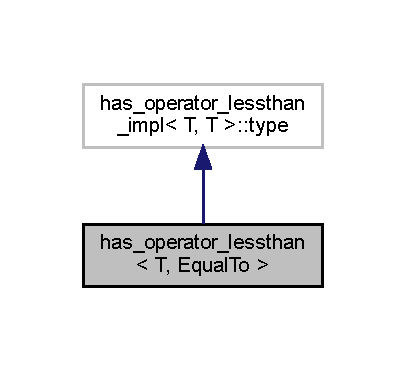
\includegraphics[width=211pt]{structhas__operator__lessthan__inherit__graph}
\end{center}
\end{figure}


Collaboration diagram for has\+\_\+operator\+\_\+lessthan$<$ T, Equal\+To $>$\+:\nopagebreak
\begin{figure}[H]
\begin{center}
\leavevmode
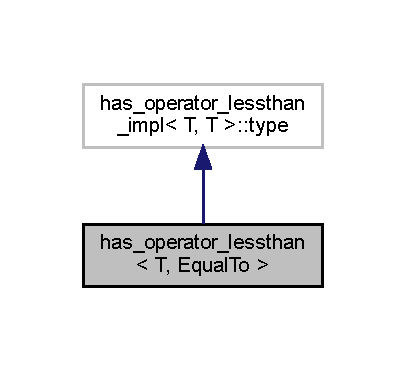
\includegraphics[width=211pt]{structhas__operator__lessthan__coll__graph}
\end{center}
\end{figure}


The documentation for this struct was generated from the following file\+:\begin{DoxyCompactItemize}
\item 
src/\+Virtual\+Machine/\hyperlink{_virtual_machine_state_8h}{Virtual\+Machine\+State.\+h}\end{DoxyCompactItemize}

\hypertarget{structhas__operator__lessthan__impl}{}\section{has\+\_\+operator\+\_\+lessthan\+\_\+impl$<$ T, Equal\+To $>$ Class Template Reference}
\label{structhas__operator__lessthan__impl}\index{has\+\_\+operator\+\_\+lessthan\+\_\+impl$<$ T, Equal\+To $>$@{has\+\_\+operator\+\_\+lessthan\+\_\+impl$<$ T, Equal\+To $>$}}


{\ttfamily \#include $<$Virtual\+Machine\+State.\+h$>$}

\subsection*{Public Types}
\begin{DoxyCompactItemize}
\item 
using \hyperlink{structhas__operator__lessthan__impl_a94158125949ce4db0eefedbdc4cbad73}{type} = typename std\+::is\+\_\+same$<$ bool, decltype(\hyperlink{structhas__operator__lessthan__impl_a5eee8607153dcb4ac5ed91df37251062}{test}$<$ T, Equal\+To $>$(0))$>$\+::\hyperlink{structhas__operator__lessthan__impl_a94158125949ce4db0eefedbdc4cbad73}{type}
\end{DoxyCompactItemize}
\subsection*{Static Public Member Functions}
\begin{DoxyCompactItemize}
\item 
{\footnotesize template$<$class U , class V $>$ }\\static auto \hyperlink{structhas__operator__lessthan__impl_a5eee8607153dcb4ac5ed91df37251062}{test} (U $\ast$) -\/$>$ decltype(std\+::declval$<$ U $>$()$<$ std\+::declval$<$ V $>$())
\item 
{\footnotesize template$<$typename , typename $>$ }\\static auto \hyperlink{structhas__operator__lessthan__impl_ae64af96a16053f6ded781dda66fc5fb1}{test} (...) -\/$>$ std\+::false\+\_\+type
\end{DoxyCompactItemize}


\subsection{Detailed Description}
\subsubsection*{template$<$class T, class Equal\+To$>$\newline
class has\+\_\+operator\+\_\+lessthan\+\_\+impl$<$ T, Equal\+To $>$}

\begin{DoxyAuthor}{Author}
piantado 
\end{DoxyAuthor}
\begin{DoxyDate}{Date}
07/05/20 
\end{DoxyDate}


\subsection{Member Typedef Documentation}
\mbox{\Hypertarget{structhas__operator__lessthan__impl_a94158125949ce4db0eefedbdc4cbad73}\label{structhas__operator__lessthan__impl_a94158125949ce4db0eefedbdc4cbad73}} 
\index{has\+\_\+operator\+\_\+lessthan\+\_\+impl@{has\+\_\+operator\+\_\+lessthan\+\_\+impl}!type@{type}}
\index{type@{type}!has\+\_\+operator\+\_\+lessthan\+\_\+impl@{has\+\_\+operator\+\_\+lessthan\+\_\+impl}}
\subsubsection{\texorpdfstring{type}{type}}
{\footnotesize\ttfamily template$<$class T, class Equal\+To$>$ \\
using \hyperlink{structhas__operator__lessthan__impl}{has\+\_\+operator\+\_\+lessthan\+\_\+impl}$<$ T, Equal\+To $>$\+::\hyperlink{structhas__operator__lessthan__impl_a94158125949ce4db0eefedbdc4cbad73}{type} =  typename std\+::is\+\_\+same$<$bool, decltype(\hyperlink{structhas__operator__lessthan__impl_a5eee8607153dcb4ac5ed91df37251062}{test}$<$T, Equal\+To$>$(0))$>$\+::\hyperlink{structhas__operator__lessthan__impl_a94158125949ce4db0eefedbdc4cbad73}{type}}



\subsection{Member Function Documentation}
\mbox{\Hypertarget{structhas__operator__lessthan__impl_a5eee8607153dcb4ac5ed91df37251062}\label{structhas__operator__lessthan__impl_a5eee8607153dcb4ac5ed91df37251062}} 
\index{has\+\_\+operator\+\_\+lessthan\+\_\+impl@{has\+\_\+operator\+\_\+lessthan\+\_\+impl}!test@{test}}
\index{test@{test}!has\+\_\+operator\+\_\+lessthan\+\_\+impl@{has\+\_\+operator\+\_\+lessthan\+\_\+impl}}
\subsubsection{\texorpdfstring{test()}{test()}\hspace{0.1cm}{\footnotesize\ttfamily [1/2]}}
{\footnotesize\ttfamily template$<$class T, class Equal\+To$>$ \\
template$<$class U , class V $>$ \\
static auto \hyperlink{structhas__operator__lessthan__impl}{has\+\_\+operator\+\_\+lessthan\+\_\+impl}$<$ T, Equal\+To $>$\+::test (\begin{DoxyParamCaption}\item[{U $\ast$}]{ }\end{DoxyParamCaption}) -\/$>$  decltype(std\+::declval$<$ U $>$()$<$ std\+::declval$<$ V $>$())\hspace{0.3cm}{\ttfamily [static]}}

\mbox{\Hypertarget{structhas__operator__lessthan__impl_ae64af96a16053f6ded781dda66fc5fb1}\label{structhas__operator__lessthan__impl_ae64af96a16053f6ded781dda66fc5fb1}} 
\index{has\+\_\+operator\+\_\+lessthan\+\_\+impl@{has\+\_\+operator\+\_\+lessthan\+\_\+impl}!test@{test}}
\index{test@{test}!has\+\_\+operator\+\_\+lessthan\+\_\+impl@{has\+\_\+operator\+\_\+lessthan\+\_\+impl}}
\subsubsection{\texorpdfstring{test()}{test()}\hspace{0.1cm}{\footnotesize\ttfamily [2/2]}}
{\footnotesize\ttfamily template$<$class T, class Equal\+To$>$ \\
template$<$typename , typename $>$ \\
static auto \hyperlink{structhas__operator__lessthan__impl}{has\+\_\+operator\+\_\+lessthan\+\_\+impl}$<$ T, Equal\+To $>$\+::test (\begin{DoxyParamCaption}\item[{}]{... }\end{DoxyParamCaption}) -\/$>$  std\+::false\+\_\+type\hspace{0.3cm}{\ttfamily [static]}}



The documentation for this class was generated from the following file\+:\begin{DoxyCompactItemize}
\item 
src/\+Virtual\+Machine/\hyperlink{_virtual_machine_state_8h}{Virtual\+Machine\+State.\+h}\end{DoxyCompactItemize}

\hypertarget{struct_has_posterior}{}\section{Has\+Posterior$<$ T, typename $>$ Class Template Reference}
\label{struct_has_posterior}\index{Has\+Posterior$<$ T, typename $>$@{Has\+Posterior$<$ T, typename $>$}}


{\ttfamily \#include $<$Top.\+h$>$}



Inheritance diagram for Has\+Posterior$<$ T, typename $>$\+:
\nopagebreak
\begin{figure}[H]
\begin{center}
\leavevmode
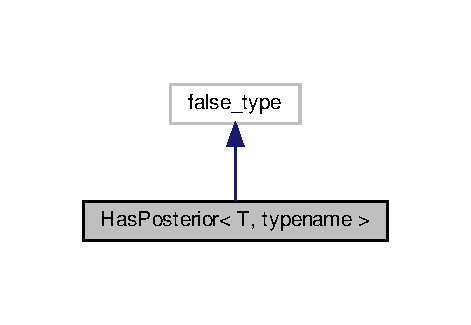
\includegraphics[width=226pt]{struct_has_posterior__inherit__graph}
\end{center}
\end{figure}


Collaboration diagram for Has\+Posterior$<$ T, typename $>$\+:
\nopagebreak
\begin{figure}[H]
\begin{center}
\leavevmode
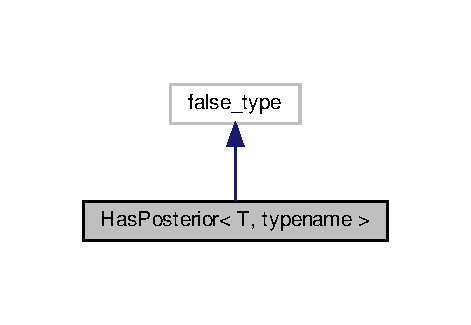
\includegraphics[width=226pt]{struct_has_posterior__coll__graph}
\end{center}
\end{figure}


\subsection{Detailed Description}
\subsubsection*{template$<$typename T, typename = double$>$\newline
class Has\+Posterior$<$ T, typename $>$}

\begin{DoxyAuthor}{Author}
piantado 
\end{DoxyAuthor}
\begin{DoxyDate}{Date}
07/05/20 
\end{DoxyDate}


The documentation for this class was generated from the following file\+:\begin{DoxyCompactItemize}
\item 
src/\+Containers/\hyperlink{_top_8h}{Top.\+h}\end{DoxyCompactItemize}

\hypertarget{struct_has_posterior_3_01_t_00_01decltype_07_07void_08_01_t_1_1posterior_00_010_08_4}{}\doxysection{Has\+Posterior$<$ T, decltype((void) T\+::posterior, 0)$>$ Struct Template Reference}
\label{struct_has_posterior_3_01_t_00_01decltype_07_07void_08_01_t_1_1posterior_00_010_08_4}\index{HasPosterior$<$ T, decltype((void) T::posterior, 0)$>$@{HasPosterior$<$ T, decltype((void) T::posterior, 0)$>$}}


{\ttfamily \#include $<$Top.\+h$>$}



Inheritance diagram for Has\+Posterior$<$ T, decltype((void) T\+::posterior, 0)$>$\+:\nopagebreak
\begin{figure}[H]
\begin{center}
\leavevmode
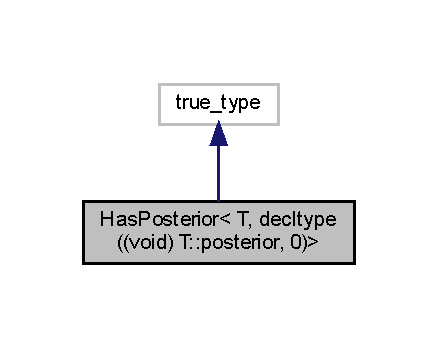
\includegraphics[width=210pt]{struct_has_posterior_3_01_t_00_01decltype_07_07void_08_01_t_1_1posterior_00_010_08_4__inherit__graph}
\end{center}
\end{figure}


Collaboration diagram for Has\+Posterior$<$ T, decltype((void) T\+::posterior, 0)$>$\+:\nopagebreak
\begin{figure}[H]
\begin{center}
\leavevmode
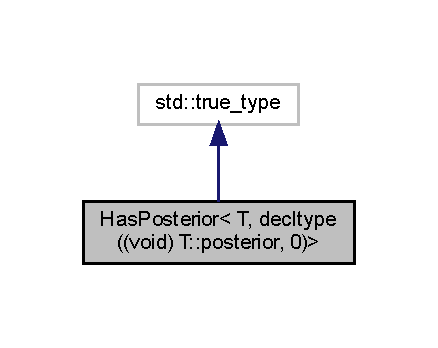
\includegraphics[width=210pt]{struct_has_posterior_3_01_t_00_01decltype_07_07void_08_01_t_1_1posterior_00_010_08_4__coll__graph}
\end{center}
\end{figure}


The documentation for this struct was generated from the following file\+:\begin{DoxyCompactItemize}
\item 
src/\+Containers/\mbox{\hyperlink{_top_8h}{Top.\+h}}\end{DoxyCompactItemize}

\hypertarget{struct_head_if_reference_else_t}{}\section{Head\+If\+Reference\+ElseT$<$ T, args $>$ Class Template Reference}
\label{struct_head_if_reference_else_t}\index{Head\+If\+Reference\+Else\+T$<$ T, args $>$@{Head\+If\+Reference\+Else\+T$<$ T, args $>$}}


{\ttfamily \#include $<$Primitives.\+h$>$}

\subsection*{Public Types}
\begin{DoxyCompactItemize}
\item 
typedef std\+::conditional$<$ std\+::is\+\_\+reference$<$ typename \hyperlink{struct_type_head}{Type\+Head}$<$ args... $>$\+::\hyperlink{struct_head_if_reference_else_t_aa668af542560a9a8541b1ff59f23d51a}{type} $>$\+::value, typename std\+::decay$<$ typename \hyperlink{struct_type_head}{Type\+Head}$<$ args... $>$\+::\hyperlink{struct_head_if_reference_else_t_aa668af542560a9a8541b1ff59f23d51a}{type} $>$\+::\hyperlink{struct_head_if_reference_else_t_aa668af542560a9a8541b1ff59f23d51a}{type}, T $>$\+::\hyperlink{struct_head_if_reference_else_t_aa668af542560a9a8541b1ff59f23d51a}{type} \hyperlink{struct_head_if_reference_else_t_aa668af542560a9a8541b1ff59f23d51a}{type}
\end{DoxyCompactItemize}


\subsection{Detailed Description}
\subsubsection*{template$<$class T, class... args$>$\newline
class Head\+If\+Reference\+Else\+T$<$ T, args $>$}

\begin{DoxyAuthor}{Author}
piantado 
\end{DoxyAuthor}
\begin{DoxyDate}{Date}
07/05/20 
\end{DoxyDate}


\subsection{Member Typedef Documentation}
\mbox{\Hypertarget{struct_head_if_reference_else_t_aa668af542560a9a8541b1ff59f23d51a}\label{struct_head_if_reference_else_t_aa668af542560a9a8541b1ff59f23d51a}} 
\index{Head\+If\+Reference\+ElseT@{Head\+If\+Reference\+ElseT}!type@{type}}
\index{type@{type}!Head\+If\+Reference\+ElseT@{Head\+If\+Reference\+ElseT}}
\subsubsection{\texorpdfstring{type}{type}}
{\footnotesize\ttfamily template$<$class T , class... args$>$ \\
typedef std\+::conditional$<$std\+::is\+\_\+reference$<$typename \hyperlink{struct_type_head}{Type\+Head}$<$args...$>$\+::\hyperlink{struct_head_if_reference_else_t_aa668af542560a9a8541b1ff59f23d51a}{type}$>$\+::value, typename std\+::decay$<$typename \hyperlink{struct_type_head}{Type\+Head}$<$args...$>$\+::\hyperlink{struct_head_if_reference_else_t_aa668af542560a9a8541b1ff59f23d51a}{type}$>$\+::\hyperlink{struct_head_if_reference_else_t_aa668af542560a9a8541b1ff59f23d51a}{type}, T $>$\+::\hyperlink{struct_head_if_reference_else_t_aa668af542560a9a8541b1ff59f23d51a}{type} \hyperlink{struct_head_if_reference_else_t}{Head\+If\+Reference\+ElseT}$<$ T, args $>$\+::\hyperlink{struct_head_if_reference_else_t_aa668af542560a9a8541b1ff59f23d51a}{type}}



The documentation for this class was generated from the following file\+:\begin{DoxyCompactItemize}
\item 
src/\+Virtual\+Machine/\hyperlink{_primitives_8h}{Primitives.\+h}\end{DoxyCompactItemize}

\hypertarget{struct_head_if_reference_else_t_3_01_t_01_4}{}\section{Head\+If\+Reference\+ElseT$<$ T $>$ Struct Template Reference}
\label{struct_head_if_reference_else_t_3_01_t_01_4}\index{Head\+If\+Reference\+Else\+T$<$ T $>$@{Head\+If\+Reference\+Else\+T$<$ T $>$}}


{\ttfamily \#include $<$Primitives.\+h$>$}

\subsection*{Public Types}
\begin{DoxyCompactItemize}
\item 
typedef T \hyperlink{struct_head_if_reference_else_t_3_01_t_01_4_ad4fabe2100fa4371e776a7ad1f75a46e}{type}
\end{DoxyCompactItemize}


\subsection{Member Typedef Documentation}
\mbox{\Hypertarget{struct_head_if_reference_else_t_3_01_t_01_4_ad4fabe2100fa4371e776a7ad1f75a46e}\label{struct_head_if_reference_else_t_3_01_t_01_4_ad4fabe2100fa4371e776a7ad1f75a46e}} 
\index{Head\+If\+Reference\+Else\+T$<$ T $>$@{Head\+If\+Reference\+Else\+T$<$ T $>$}!type@{type}}
\index{type@{type}!Head\+If\+Reference\+Else\+T$<$ T $>$@{Head\+If\+Reference\+Else\+T$<$ T $>$}}
\subsubsection{\texorpdfstring{type}{type}}
{\footnotesize\ttfamily template$<$class T $>$ \\
typedef T \hyperlink{struct_head_if_reference_else_t}{Head\+If\+Reference\+ElseT}$<$ T $>$\+::\hyperlink{struct_head_if_reference_else_t_3_01_t_01_4_ad4fabe2100fa4371e776a7ad1f75a46e}{type}}



The documentation for this struct was generated from the following file\+:\begin{DoxyCompactItemize}
\item 
src/\+Virtual\+Machine/\hyperlink{_primitives_8h}{Primitives.\+h}\end{DoxyCompactItemize}

\hypertarget{struct_human_datum}{}\doxysection{Human\+Datum$<$ H\+YP, \+\_\+output\+\_\+t, \+\_\+datum\+\_\+t, \+\_\+data\+\_\+t $>$ Class Template Reference}
\label{struct_human_datum}\index{HumanDatum$<$ HYP, \_output\_t, \_datum\_t, \_data\_t $>$@{HumanDatum$<$ HYP, \_output\_t, \_datum\_t, \_data\_t $>$}}


{\ttfamily \#include $<$Human\+Datum.\+h$>$}

\doxysubsection*{Public Types}
\begin{DoxyCompactItemize}
\item 
typedef \+\_\+data\+\_\+t \mbox{\hyperlink{struct_human_datum_ad442cb9ab3d48a298c8e92b36099d049}{data\+\_\+t}}
\item 
typedef \+\_\+datum\+\_\+t \mbox{\hyperlink{struct_human_datum_ac25e73a87ace1bdfdf24a5c950b08f4f}{datum\+\_\+t}}
\item 
typedef \+\_\+output\+\_\+t \mbox{\hyperlink{struct_human_datum_a15c95575a11867683feff4437fc90b98}{output\+\_\+t}}
\end{DoxyCompactItemize}
\doxysubsection*{Public Attributes}
\begin{DoxyCompactItemize}
\item 
\mbox{\hyperlink{struct_human_datum_ad442cb9ab3d48a298c8e92b36099d049}{data\+\_\+t}} $\ast$ \mbox{\hyperlink{struct_human_datum_aaf85efe4e8529282096c1331f24b61b1}{data}}
\item 
size\+\_\+t \mbox{\hyperlink{struct_human_datum_a1dcceba908420f512da7b2b2fc1247fe}{ndata}}
\item 
\mbox{\hyperlink{struct_human_datum_ac25e73a87ace1bdfdf24a5c950b08f4f}{datum\+\_\+t}} $\ast$ \mbox{\hyperlink{struct_human_datum_ae82de9e30e32e86b013dd3ebf475eb71}{predict}}
\item 
std\+::map$<$ \mbox{\hyperlink{struct_human_datum_a15c95575a11867683feff4437fc90b98}{output\+\_\+t}}, size\+\_\+t $>$ \mbox{\hyperlink{struct_human_datum_aad2be31d72b759b1c7a15631bc07993f}{responses}}
\item 
double \mbox{\hyperlink{struct_human_datum_ac1c5eb254faf89b76e8d040da8daa930}{chance}}
\item 
int \mbox{\hyperlink{struct_human_datum_a72c3ad2a4442b67dd2b39c3008f89c3d}{decay\+\_\+position}}
\end{DoxyCompactItemize}


\doxysubsection{Detailed Description}
\subsubsection*{template$<$typename H\+YP, typename \+\_\+output\+\_\+t = H\+Y\+P\+::output\+\_\+t, typename \+\_\+datum\+\_\+t = H\+Y\+P\+::datum\+\_\+t, typename \+\_\+data\+\_\+t = H\+Y\+P\+::data\+\_\+t$>$\newline
class Human\+Datum$<$ H\+Y\+P, \+\_\+output\+\_\+t, \+\_\+datum\+\_\+t, \+\_\+data\+\_\+t $>$}

\begin{DoxyAuthor}{Author}
piantado 
\end{DoxyAuthor}
\begin{DoxyDate}{Date}
03/08/20 
\end{DoxyDate}


\doxysubsection{Member Typedef Documentation}
\mbox{\Hypertarget{struct_human_datum_ad442cb9ab3d48a298c8e92b36099d049}\label{struct_human_datum_ad442cb9ab3d48a298c8e92b36099d049}} 
\index{HumanDatum$<$ HYP, \_output\_t, \_datum\_t, \_data\_t $>$@{HumanDatum$<$ HYP, \_output\_t, \_datum\_t, \_data\_t $>$}!data\_t@{data\_t}}
\index{data\_t@{data\_t}!HumanDatum$<$ HYP, \_output\_t, \_datum\_t, \_data\_t $>$@{HumanDatum$<$ HYP, \_output\_t, \_datum\_t, \_data\_t $>$}}
\doxysubsubsection{\texorpdfstring{data\_t}{data\_t}}
{\footnotesize\ttfamily template$<$typename H\+YP , typename \+\_\+output\+\_\+t  = H\+Y\+P\+::output\+\_\+t, typename \+\_\+datum\+\_\+t  = H\+Y\+P\+::datum\+\_\+t, typename \+\_\+data\+\_\+t  = H\+Y\+P\+::data\+\_\+t$>$ \\
typedef \+\_\+data\+\_\+t \mbox{\hyperlink{struct_human_datum}{Human\+Datum}}$<$ H\+YP, \+\_\+output\+\_\+t, \+\_\+datum\+\_\+t, \+\_\+data\+\_\+t $>$\+::\mbox{\hyperlink{struct_human_datum_ad442cb9ab3d48a298c8e92b36099d049}{data\+\_\+t}}}

\mbox{\Hypertarget{struct_human_datum_ac25e73a87ace1bdfdf24a5c950b08f4f}\label{struct_human_datum_ac25e73a87ace1bdfdf24a5c950b08f4f}} 
\index{HumanDatum$<$ HYP, \_output\_t, \_datum\_t, \_data\_t $>$@{HumanDatum$<$ HYP, \_output\_t, \_datum\_t, \_data\_t $>$}!datum\_t@{datum\_t}}
\index{datum\_t@{datum\_t}!HumanDatum$<$ HYP, \_output\_t, \_datum\_t, \_data\_t $>$@{HumanDatum$<$ HYP, \_output\_t, \_datum\_t, \_data\_t $>$}}
\doxysubsubsection{\texorpdfstring{datum\_t}{datum\_t}}
{\footnotesize\ttfamily template$<$typename H\+YP , typename \+\_\+output\+\_\+t  = H\+Y\+P\+::output\+\_\+t, typename \+\_\+datum\+\_\+t  = H\+Y\+P\+::datum\+\_\+t, typename \+\_\+data\+\_\+t  = H\+Y\+P\+::data\+\_\+t$>$ \\
typedef \+\_\+datum\+\_\+t \mbox{\hyperlink{struct_human_datum}{Human\+Datum}}$<$ H\+YP, \+\_\+output\+\_\+t, \+\_\+datum\+\_\+t, \+\_\+data\+\_\+t $>$\+::\mbox{\hyperlink{struct_human_datum_ac25e73a87ace1bdfdf24a5c950b08f4f}{datum\+\_\+t}}}

\mbox{\Hypertarget{struct_human_datum_a15c95575a11867683feff4437fc90b98}\label{struct_human_datum_a15c95575a11867683feff4437fc90b98}} 
\index{HumanDatum$<$ HYP, \_output\_t, \_datum\_t, \_data\_t $>$@{HumanDatum$<$ HYP, \_output\_t, \_datum\_t, \_data\_t $>$}!output\_t@{output\_t}}
\index{output\_t@{output\_t}!HumanDatum$<$ HYP, \_output\_t, \_datum\_t, \_data\_t $>$@{HumanDatum$<$ HYP, \_output\_t, \_datum\_t, \_data\_t $>$}}
\doxysubsubsection{\texorpdfstring{output\_t}{output\_t}}
{\footnotesize\ttfamily template$<$typename H\+YP , typename \+\_\+output\+\_\+t  = H\+Y\+P\+::output\+\_\+t, typename \+\_\+datum\+\_\+t  = H\+Y\+P\+::datum\+\_\+t, typename \+\_\+data\+\_\+t  = H\+Y\+P\+::data\+\_\+t$>$ \\
typedef \+\_\+output\+\_\+t \mbox{\hyperlink{struct_human_datum}{Human\+Datum}}$<$ H\+YP, \+\_\+output\+\_\+t, \+\_\+datum\+\_\+t, \+\_\+data\+\_\+t $>$\+::\mbox{\hyperlink{struct_human_datum_a15c95575a11867683feff4437fc90b98}{output\+\_\+t}}}



\doxysubsection{Member Data Documentation}
\mbox{\Hypertarget{struct_human_datum_ac1c5eb254faf89b76e8d040da8daa930}\label{struct_human_datum_ac1c5eb254faf89b76e8d040da8daa930}} 
\index{HumanDatum$<$ HYP, \_output\_t, \_datum\_t, \_data\_t $>$@{HumanDatum$<$ HYP, \_output\_t, \_datum\_t, \_data\_t $>$}!chance@{chance}}
\index{chance@{chance}!HumanDatum$<$ HYP, \_output\_t, \_datum\_t, \_data\_t $>$@{HumanDatum$<$ HYP, \_output\_t, \_datum\_t, \_data\_t $>$}}
\doxysubsubsection{\texorpdfstring{chance}{chance}}
{\footnotesize\ttfamily template$<$typename H\+YP , typename \+\_\+output\+\_\+t  = H\+Y\+P\+::output\+\_\+t, typename \+\_\+datum\+\_\+t  = H\+Y\+P\+::datum\+\_\+t, typename \+\_\+data\+\_\+t  = H\+Y\+P\+::data\+\_\+t$>$ \\
double \mbox{\hyperlink{struct_human_datum}{Human\+Datum}}$<$ H\+YP, \+\_\+output\+\_\+t, \+\_\+datum\+\_\+t, \+\_\+data\+\_\+t $>$\+::chance}

\mbox{\Hypertarget{struct_human_datum_aaf85efe4e8529282096c1331f24b61b1}\label{struct_human_datum_aaf85efe4e8529282096c1331f24b61b1}} 
\index{HumanDatum$<$ HYP, \_output\_t, \_datum\_t, \_data\_t $>$@{HumanDatum$<$ HYP, \_output\_t, \_datum\_t, \_data\_t $>$}!data@{data}}
\index{data@{data}!HumanDatum$<$ HYP, \_output\_t, \_datum\_t, \_data\_t $>$@{HumanDatum$<$ HYP, \_output\_t, \_datum\_t, \_data\_t $>$}}
\doxysubsubsection{\texorpdfstring{data}{data}}
{\footnotesize\ttfamily template$<$typename H\+YP , typename \+\_\+output\+\_\+t  = H\+Y\+P\+::output\+\_\+t, typename \+\_\+datum\+\_\+t  = H\+Y\+P\+::datum\+\_\+t, typename \+\_\+data\+\_\+t  = H\+Y\+P\+::data\+\_\+t$>$ \\
\mbox{\hyperlink{struct_human_datum_ad442cb9ab3d48a298c8e92b36099d049}{data\+\_\+t}}$\ast$ \mbox{\hyperlink{struct_human_datum}{Human\+Datum}}$<$ H\+YP, \+\_\+output\+\_\+t, \+\_\+datum\+\_\+t, \+\_\+data\+\_\+t $>$\+::data}

\mbox{\Hypertarget{struct_human_datum_a72c3ad2a4442b67dd2b39c3008f89c3d}\label{struct_human_datum_a72c3ad2a4442b67dd2b39c3008f89c3d}} 
\index{HumanDatum$<$ HYP, \_output\_t, \_datum\_t, \_data\_t $>$@{HumanDatum$<$ HYP, \_output\_t, \_datum\_t, \_data\_t $>$}!decay\_position@{decay\_position}}
\index{decay\_position@{decay\_position}!HumanDatum$<$ HYP, \_output\_t, \_datum\_t, \_data\_t $>$@{HumanDatum$<$ HYP, \_output\_t, \_datum\_t, \_data\_t $>$}}
\doxysubsubsection{\texorpdfstring{decay\_position}{decay\_position}}
{\footnotesize\ttfamily template$<$typename H\+YP , typename \+\_\+output\+\_\+t  = H\+Y\+P\+::output\+\_\+t, typename \+\_\+datum\+\_\+t  = H\+Y\+P\+::datum\+\_\+t, typename \+\_\+data\+\_\+t  = H\+Y\+P\+::data\+\_\+t$>$ \\
int \mbox{\hyperlink{struct_human_datum}{Human\+Datum}}$<$ H\+YP, \+\_\+output\+\_\+t, \+\_\+datum\+\_\+t, \+\_\+data\+\_\+t $>$\+::decay\+\_\+position}

\mbox{\Hypertarget{struct_human_datum_a1dcceba908420f512da7b2b2fc1247fe}\label{struct_human_datum_a1dcceba908420f512da7b2b2fc1247fe}} 
\index{HumanDatum$<$ HYP, \_output\_t, \_datum\_t, \_data\_t $>$@{HumanDatum$<$ HYP, \_output\_t, \_datum\_t, \_data\_t $>$}!ndata@{ndata}}
\index{ndata@{ndata}!HumanDatum$<$ HYP, \_output\_t, \_datum\_t, \_data\_t $>$@{HumanDatum$<$ HYP, \_output\_t, \_datum\_t, \_data\_t $>$}}
\doxysubsubsection{\texorpdfstring{ndata}{ndata}}
{\footnotesize\ttfamily template$<$typename H\+YP , typename \+\_\+output\+\_\+t  = H\+Y\+P\+::output\+\_\+t, typename \+\_\+datum\+\_\+t  = H\+Y\+P\+::datum\+\_\+t, typename \+\_\+data\+\_\+t  = H\+Y\+P\+::data\+\_\+t$>$ \\
size\+\_\+t \mbox{\hyperlink{struct_human_datum}{Human\+Datum}}$<$ H\+YP, \+\_\+output\+\_\+t, \+\_\+datum\+\_\+t, \+\_\+data\+\_\+t $>$\+::ndata}

\mbox{\Hypertarget{struct_human_datum_ae82de9e30e32e86b013dd3ebf475eb71}\label{struct_human_datum_ae82de9e30e32e86b013dd3ebf475eb71}} 
\index{HumanDatum$<$ HYP, \_output\_t, \_datum\_t, \_data\_t $>$@{HumanDatum$<$ HYP, \_output\_t, \_datum\_t, \_data\_t $>$}!predict@{predict}}
\index{predict@{predict}!HumanDatum$<$ HYP, \_output\_t, \_datum\_t, \_data\_t $>$@{HumanDatum$<$ HYP, \_output\_t, \_datum\_t, \_data\_t $>$}}
\doxysubsubsection{\texorpdfstring{predict}{predict}}
{\footnotesize\ttfamily template$<$typename H\+YP , typename \+\_\+output\+\_\+t  = H\+Y\+P\+::output\+\_\+t, typename \+\_\+datum\+\_\+t  = H\+Y\+P\+::datum\+\_\+t, typename \+\_\+data\+\_\+t  = H\+Y\+P\+::data\+\_\+t$>$ \\
\mbox{\hyperlink{struct_human_datum_ac25e73a87ace1bdfdf24a5c950b08f4f}{datum\+\_\+t}}$\ast$ \mbox{\hyperlink{struct_human_datum}{Human\+Datum}}$<$ H\+YP, \+\_\+output\+\_\+t, \+\_\+datum\+\_\+t, \+\_\+data\+\_\+t $>$\+::predict}

\mbox{\Hypertarget{struct_human_datum_aad2be31d72b759b1c7a15631bc07993f}\label{struct_human_datum_aad2be31d72b759b1c7a15631bc07993f}} 
\index{HumanDatum$<$ HYP, \_output\_t, \_datum\_t, \_data\_t $>$@{HumanDatum$<$ HYP, \_output\_t, \_datum\_t, \_data\_t $>$}!responses@{responses}}
\index{responses@{responses}!HumanDatum$<$ HYP, \_output\_t, \_datum\_t, \_data\_t $>$@{HumanDatum$<$ HYP, \_output\_t, \_datum\_t, \_data\_t $>$}}
\doxysubsubsection{\texorpdfstring{responses}{responses}}
{\footnotesize\ttfamily template$<$typename H\+YP , typename \+\_\+output\+\_\+t  = H\+Y\+P\+::output\+\_\+t, typename \+\_\+datum\+\_\+t  = H\+Y\+P\+::datum\+\_\+t, typename \+\_\+data\+\_\+t  = H\+Y\+P\+::data\+\_\+t$>$ \\
std\+::map$<$\mbox{\hyperlink{struct_human_datum_a15c95575a11867683feff4437fc90b98}{output\+\_\+t}},size\+\_\+t$>$ \mbox{\hyperlink{struct_human_datum}{Human\+Datum}}$<$ H\+YP, \+\_\+output\+\_\+t, \+\_\+datum\+\_\+t, \+\_\+data\+\_\+t $>$\+::responses}



The documentation for this class was generated from the following file\+:\begin{DoxyCompactItemize}
\item 
src/\+Data/\mbox{\hyperlink{_human_datum_8h}{Human\+Datum.\+h}}\end{DoxyCompactItemize}

\hypertarget{struct_builtin_1_1_if}{}\section{Builtin\+:\+:If$<$ t $>$ Struct Template Reference}
\label{struct_builtin_1_1_if}\index{Builtin\+::\+If$<$ t $>$@{Builtin\+::\+If$<$ t $>$}}


{\ttfamily \#include $<$Builtins.\+h$>$}



Inheritance diagram for Builtin\+:\+:If$<$ t $>$\+:\nopagebreak
\begin{figure}[H]
\begin{center}
\leavevmode
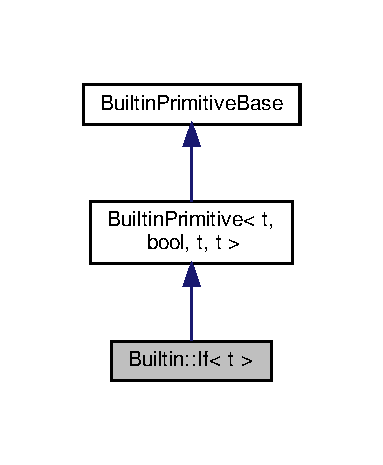
\includegraphics[width=184pt]{struct_builtin_1_1_if__inherit__graph}
\end{center}
\end{figure}


Collaboration diagram for Builtin\+:\+:If$<$ t $>$\+:\nopagebreak
\begin{figure}[H]
\begin{center}
\leavevmode
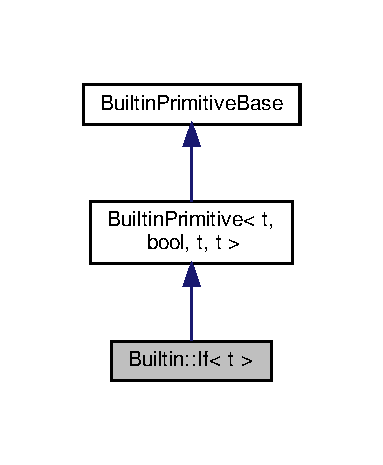
\includegraphics[width=184pt]{struct_builtin_1_1_if__coll__graph}
\end{center}
\end{figure}
\subsection*{Public Member Functions}
\begin{DoxyCompactItemize}
\item 
\hyperlink{struct_builtin_1_1_if_a4ea649fb18a5c42445c5c48e8549c951}{If} (std\+::string fmt, double \+\_\+p=1.\+0)
\end{DoxyCompactItemize}
\subsection*{Additional Inherited Members}


\subsection{Constructor \& Destructor Documentation}
\mbox{\Hypertarget{struct_builtin_1_1_if_a4ea649fb18a5c42445c5c48e8549c951}\label{struct_builtin_1_1_if_a4ea649fb18a5c42445c5c48e8549c951}} 
\index{Builtin\+::\+If@{Builtin\+::\+If}!If@{If}}
\index{If@{If}!Builtin\+::\+If@{Builtin\+::\+If}}
\subsubsection{\texorpdfstring{If()}{If()}}
{\footnotesize\ttfamily template$<$typename t $>$ \\
\hyperlink{struct_builtin_1_1_if}{Builtin\+::\+If}$<$ t $>$\+::\hyperlink{struct_builtin_1_1_if}{If} (\begin{DoxyParamCaption}\item[{std\+::string}]{fmt,  }\item[{double}]{\+\_\+p = {\ttfamily 1.0} }\end{DoxyParamCaption})\hspace{0.3cm}{\ttfamily [inline]}}



The documentation for this struct was generated from the following file\+:\begin{DoxyCompactItemize}
\item 
src/\+Virtual\+Machine/\hyperlink{_builtins_8h}{Builtins.\+h}\end{DoxyCompactItemize}

\hypertarget{class_inferece_interface}{}\section{Inferece\+Interface Class Reference}
\label{class_inferece_interface}\index{Inferece\+Interface@{Inferece\+Interface}}


{\ttfamily \#include $<$Parallel\+Inference\+Interface.\+h$>$}



\subsection{Detailed Description}
\begin{DoxyAuthor}{Author}
piantado 
\end{DoxyAuthor}
\begin{DoxyDate}{Date}
07/06/20 
\end{DoxyDate}


The documentation for this class was generated from the following file\+:\begin{DoxyCompactItemize}
\item 
src/\+Inference/\hyperlink{_parallel_inference_interface_8h}{Parallel\+Inference\+Interface.\+h}\end{DoxyCompactItemize}

\hypertarget{class_instruction}{}\section{Instruction Class Reference}
\label{class_instruction}\index{Instruction@{Instruction}}


{\ttfamily \#include $<$Instruction.\+h$>$}

\subsection*{Public Member Functions}
\begin{DoxyCompactItemize}
\item 
\hyperlink{class_instruction_aebd15229c1651af49dcb203707e7a2d5}{Instruction} ()
\item 
\hyperlink{class_instruction_a7f672d88ba4ec174716bbac9adb8b1b0}{Instruction} (\hyperlink{_instruction_8h_af2fb7c87c5854c5733d7bb0506b06de7}{Builtin\+Op} x, int arg\+\_\+=0x0)
\item 
\hyperlink{class_instruction_a62d7782f809fa55635a6ced1e971eb3b}{Instruction} (\hyperlink{_instruction_8h_a227278394efd1e2313c727102db09ea9}{Primitive\+Op} x, int arg\+\_\+=0x0)
\item 
{\footnotesize template$<$typename t $>$ }\\bool \hyperlink{class_instruction_ade73e12471250fd191362d462e2f4970}{is} () const
\item 
{\footnotesize template$<$typename t $>$ }\\t \hyperlink{class_instruction_ac99272000afeb9015a9d40ceed8c139b}{as} () const
\item 
int \hyperlink{class_instruction_a83a2763aa1dab5281b27dd99925f683e}{get\+Arg} () const
\item 
bool \hyperlink{class_instruction_a75e0ecee9ec917bcc47488a1fbeb6a24}{operator==} (const \hyperlink{class_instruction}{Instruction} \&i) const
\item 
{\footnotesize template$<$typename T $>$ }\\bool \hyperlink{class_instruction_a924203cd9a0516d64556ecbf6a79df8a}{is\+\_\+a} (const T x) const
\begin{DoxyCompactList}\small\item\em compare the instruction types (ignores the arg) \end{DoxyCompactList}\item 
{\footnotesize template$<$typename T , typename... Ts$>$ }\\bool \hyperlink{class_instruction_ae670ee58f9acdfd60b7213f77dfca794}{is\+\_\+a} (T x, Ts... args) const
\end{DoxyCompactItemize}
\subsection*{Public Attributes}
\begin{DoxyCompactItemize}
\item 
std\+::variant$<$ \hyperlink{_instruction_8h_af2fb7c87c5854c5733d7bb0506b06de7}{Builtin\+Op}, \hyperlink{_instruction_8h_a227278394efd1e2313c727102db09ea9}{Primitive\+Op} $>$ \hyperlink{class_instruction_ad6b1f252f404568d2fe80644a7caa224}{op}
\item 
int \hyperlink{class_instruction_a7ed399e29ec58e97a7b6311919f5d5ca}{arg}
\end{DoxyCompactItemize}


\subsection{Detailed Description}
\begin{DoxyAuthor}{Author}
piantado 
\end{DoxyAuthor}
\begin{DoxyDate}{Date}
29/01/20 
\end{DoxyDate}


\subsection{Constructor \& Destructor Documentation}
\mbox{\Hypertarget{class_instruction_aebd15229c1651af49dcb203707e7a2d5}\label{class_instruction_aebd15229c1651af49dcb203707e7a2d5}} 
\index{Instruction@{Instruction}!Instruction@{Instruction}}
\index{Instruction@{Instruction}!Instruction@{Instruction}}
\subsubsection{\texorpdfstring{Instruction()}{Instruction()}\hspace{0.1cm}{\footnotesize\ttfamily [1/3]}}
{\footnotesize\ttfamily Instruction\+::\+Instruction (\begin{DoxyParamCaption}{ }\end{DoxyParamCaption})\hspace{0.3cm}{\ttfamily [inline]}}

\mbox{\Hypertarget{class_instruction_a7f672d88ba4ec174716bbac9adb8b1b0}\label{class_instruction_a7f672d88ba4ec174716bbac9adb8b1b0}} 
\index{Instruction@{Instruction}!Instruction@{Instruction}}
\index{Instruction@{Instruction}!Instruction@{Instruction}}
\subsubsection{\texorpdfstring{Instruction()}{Instruction()}\hspace{0.1cm}{\footnotesize\ttfamily [2/3]}}
{\footnotesize\ttfamily Instruction\+::\+Instruction (\begin{DoxyParamCaption}\item[{\hyperlink{_instruction_8h_af2fb7c87c5854c5733d7bb0506b06de7}{Builtin\+Op}}]{x,  }\item[{int}]{arg\+\_\+ = {\ttfamily 0x0} }\end{DoxyParamCaption})\hspace{0.3cm}{\ttfamily [inline]}}

\mbox{\Hypertarget{class_instruction_a62d7782f809fa55635a6ced1e971eb3b}\label{class_instruction_a62d7782f809fa55635a6ced1e971eb3b}} 
\index{Instruction@{Instruction}!Instruction@{Instruction}}
\index{Instruction@{Instruction}!Instruction@{Instruction}}
\subsubsection{\texorpdfstring{Instruction()}{Instruction()}\hspace{0.1cm}{\footnotesize\ttfamily [3/3]}}
{\footnotesize\ttfamily Instruction\+::\+Instruction (\begin{DoxyParamCaption}\item[{\hyperlink{_instruction_8h_a227278394efd1e2313c727102db09ea9}{Primitive\+Op}}]{x,  }\item[{int}]{arg\+\_\+ = {\ttfamily 0x0} }\end{DoxyParamCaption})\hspace{0.3cm}{\ttfamily [inline]}}



\subsection{Member Function Documentation}
\mbox{\Hypertarget{class_instruction_ac99272000afeb9015a9d40ceed8c139b}\label{class_instruction_ac99272000afeb9015a9d40ceed8c139b}} 
\index{Instruction@{Instruction}!as@{as}}
\index{as@{as}!Instruction@{Instruction}}
\subsubsection{\texorpdfstring{as()}{as()}}
{\footnotesize\ttfamily template$<$typename t $>$ \\
t Instruction\+::as (\begin{DoxyParamCaption}{ }\end{DoxyParamCaption}) const\hspace{0.3cm}{\ttfamily [inline]}}

Get as type t \begin{DoxyReturn}{Returns}

\end{DoxyReturn}
\mbox{\Hypertarget{class_instruction_a83a2763aa1dab5281b27dd99925f683e}\label{class_instruction_a83a2763aa1dab5281b27dd99925f683e}} 
\index{Instruction@{Instruction}!get\+Arg@{get\+Arg}}
\index{get\+Arg@{get\+Arg}!Instruction@{Instruction}}
\subsubsection{\texorpdfstring{get\+Arg()}{getArg()}}
{\footnotesize\ttfamily int Instruction\+::get\+Arg (\begin{DoxyParamCaption}{ }\end{DoxyParamCaption}) const\hspace{0.3cm}{\ttfamily [inline]}}

Return the argument (an int) \begin{DoxyReturn}{Returns}

\end{DoxyReturn}
\mbox{\Hypertarget{class_instruction_ade73e12471250fd191362d462e2f4970}\label{class_instruction_ade73e12471250fd191362d462e2f4970}} 
\index{Instruction@{Instruction}!is@{is}}
\index{is@{is}!Instruction@{Instruction}}
\subsubsection{\texorpdfstring{is()}{is()}}
{\footnotesize\ttfamily template$<$typename t $>$ \\
bool Instruction\+::is (\begin{DoxyParamCaption}{ }\end{DoxyParamCaption}) const\hspace{0.3cm}{\ttfamily [inline]}}

Template to check if this instruction is holding type t \begin{DoxyReturn}{Returns}

\end{DoxyReturn}
\mbox{\Hypertarget{class_instruction_a924203cd9a0516d64556ecbf6a79df8a}\label{class_instruction_a924203cd9a0516d64556ecbf6a79df8a}} 
\index{Instruction@{Instruction}!is\+\_\+a@{is\+\_\+a}}
\index{is\+\_\+a@{is\+\_\+a}!Instruction@{Instruction}}
\subsubsection{\texorpdfstring{is\+\_\+a()}{is\_a()}\hspace{0.1cm}{\footnotesize\ttfamily [1/2]}}
{\footnotesize\ttfamily template$<$typename T $>$ \\
bool Instruction\+::is\+\_\+a (\begin{DoxyParamCaption}\item[{const T}]{x }\end{DoxyParamCaption}) const\hspace{0.3cm}{\ttfamily [inline]}}



compare the instruction types (ignores the arg) 

\mbox{\Hypertarget{class_instruction_ae670ee58f9acdfd60b7213f77dfca794}\label{class_instruction_ae670ee58f9acdfd60b7213f77dfca794}} 
\index{Instruction@{Instruction}!is\+\_\+a@{is\+\_\+a}}
\index{is\+\_\+a@{is\+\_\+a}!Instruction@{Instruction}}
\subsubsection{\texorpdfstring{is\+\_\+a()}{is\_a()}\hspace{0.1cm}{\footnotesize\ttfamily [2/2]}}
{\footnotesize\ttfamily template$<$typename T , typename... Ts$>$ \\
bool Instruction\+::is\+\_\+a (\begin{DoxyParamCaption}\item[{T}]{x,  }\item[{Ts...}]{args }\end{DoxyParamCaption}) const\hspace{0.3cm}{\ttfamily [inline]}}

Variadic checking of whether this is a given op type 
\begin{DoxyParams}{Parameters}
{\em x} & \\
\hline
\end{DoxyParams}
\begin{DoxyReturn}{Returns}

\end{DoxyReturn}
\mbox{\Hypertarget{class_instruction_a75e0ecee9ec917bcc47488a1fbeb6a24}\label{class_instruction_a75e0ecee9ec917bcc47488a1fbeb6a24}} 
\index{Instruction@{Instruction}!operator==@{operator==}}
\index{operator==@{operator==}!Instruction@{Instruction}}
\subsubsection{\texorpdfstring{operator==()}{operator==()}}
{\footnotesize\ttfamily bool Instruction\+::operator== (\begin{DoxyParamCaption}\item[{const \hyperlink{class_instruction}{Instruction} \&}]{i }\end{DoxyParamCaption}) const\hspace{0.3cm}{\ttfamily [inline]}}



\subsection{Member Data Documentation}
\mbox{\Hypertarget{class_instruction_a7ed399e29ec58e97a7b6311919f5d5ca}\label{class_instruction_a7ed399e29ec58e97a7b6311919f5d5ca}} 
\index{Instruction@{Instruction}!arg@{arg}}
\index{arg@{arg}!Instruction@{Instruction}}
\subsubsection{\texorpdfstring{arg}{arg}}
{\footnotesize\ttfamily int Instruction\+::arg}

\mbox{\Hypertarget{class_instruction_ad6b1f252f404568d2fe80644a7caa224}\label{class_instruction_ad6b1f252f404568d2fe80644a7caa224}} 
\index{Instruction@{Instruction}!op@{op}}
\index{op@{op}!Instruction@{Instruction}}
\subsubsection{\texorpdfstring{op}{op}}
{\footnotesize\ttfamily std\+::variant$<$\hyperlink{_instruction_8h_af2fb7c87c5854c5733d7bb0506b06de7}{Builtin\+Op}, \hyperlink{_instruction_8h_a227278394efd1e2313c727102db09ea9}{Primitive\+Op}$>$ Instruction\+::op}



The documentation for this class was generated from the following file\+:\begin{DoxyCompactItemize}
\item 
src/\+Virtual\+Machine/\hyperlink{_instruction_8h}{Instruction.\+h}\end{DoxyCompactItemize}

\hypertarget{class_integerized_stack}{}\section{Integerized\+Stack Class Reference}
\label{class_integerized_stack}\index{Integerized\+Stack@{Integerized\+Stack}}


{\ttfamily \#include $<$Integerized\+Stack.\+h$>$}

\subsection*{Public Member Functions}
\begin{DoxyCompactItemize}
\item 
\hyperlink{class_integerized_stack_a46b24ace7ea983bfabaa437932111440}{Integerized\+Stack} (value\+\_\+t v=0)
\item 
value\+\_\+t \hyperlink{class_integerized_stack_a5edd593c74341341cc6f8e41e0f14bdf}{pop} ()
\item 
value\+\_\+t \hyperlink{class_integerized_stack_a713da8c8102cb5a53ec3ad87fada36f5}{pop} (value\+\_\+t modulus)
\item 
void \hyperlink{class_integerized_stack_a721481e52e56398bee39edf6a3d2ff80}{push} (value\+\_\+t x)
\item 
void \hyperlink{class_integerized_stack_affd28eb928362de80e35cd4e1ecdf96b}{push} (value\+\_\+t x, value\+\_\+t modulus)
\item 
value\+\_\+t \hyperlink{class_integerized_stack_aedecc57b1bbb2c056f57a00ec6eea2e3}{get\+\_\+value} () const
\item 
bool \hyperlink{class_integerized_stack_a549d4ed66e89d2e3d7e726d5c8e28fa2}{empty} () const
\item 
void \hyperlink{class_integerized_stack_a829e18dc8bae3eb371e9822271102a2d}{operator=} (value\+\_\+t z)
\item 
void \hyperlink{class_integerized_stack_ac2ec311399b327573a2c0f19d2a902a4}{operator-\/=} (value\+\_\+t x)
\item 
void \hyperlink{class_integerized_stack_a70df05b936e94c717584290d0c457cca}{operator+=} (value\+\_\+t x)
\end{DoxyCompactItemize}
\subsection*{Protected Attributes}
\begin{DoxyCompactItemize}
\item 
value\+\_\+t \hyperlink{class_integerized_stack_afcfb2d32d51c88b556f3bb7ff2544be5}{value}
\end{DoxyCompactItemize}


\subsection{Constructor \& Destructor Documentation}
\mbox{\Hypertarget{class_integerized_stack_a46b24ace7ea983bfabaa437932111440}\label{class_integerized_stack_a46b24ace7ea983bfabaa437932111440}} 
\index{Integerized\+Stack@{Integerized\+Stack}!Integerized\+Stack@{Integerized\+Stack}}
\index{Integerized\+Stack@{Integerized\+Stack}!Integerized\+Stack@{Integerized\+Stack}}
\subsubsection{\texorpdfstring{Integerized\+Stack()}{IntegerizedStack()}}
{\footnotesize\ttfamily Integerized\+Stack\+::\+Integerized\+Stack (\begin{DoxyParamCaption}\item[{value\+\_\+t}]{v = {\ttfamily 0} }\end{DoxyParamCaption})\hspace{0.3cm}{\ttfamily [inline]}}



\subsection{Member Function Documentation}
\mbox{\Hypertarget{class_integerized_stack_a549d4ed66e89d2e3d7e726d5c8e28fa2}\label{class_integerized_stack_a549d4ed66e89d2e3d7e726d5c8e28fa2}} 
\index{Integerized\+Stack@{Integerized\+Stack}!empty@{empty}}
\index{empty@{empty}!Integerized\+Stack@{Integerized\+Stack}}
\subsubsection{\texorpdfstring{empty()}{empty()}}
{\footnotesize\ttfamily bool Integerized\+Stack\+::empty (\begin{DoxyParamCaption}{ }\end{DoxyParamCaption}) const\hspace{0.3cm}{\ttfamily [inline]}}

\mbox{\Hypertarget{class_integerized_stack_aedecc57b1bbb2c056f57a00ec6eea2e3}\label{class_integerized_stack_aedecc57b1bbb2c056f57a00ec6eea2e3}} 
\index{Integerized\+Stack@{Integerized\+Stack}!get\+\_\+value@{get\+\_\+value}}
\index{get\+\_\+value@{get\+\_\+value}!Integerized\+Stack@{Integerized\+Stack}}
\subsubsection{\texorpdfstring{get\+\_\+value()}{get\_value()}}
{\footnotesize\ttfamily value\+\_\+t Integerized\+Stack\+::get\+\_\+value (\begin{DoxyParamCaption}{ }\end{DoxyParamCaption}) const\hspace{0.3cm}{\ttfamily [inline]}}

\mbox{\Hypertarget{class_integerized_stack_a70df05b936e94c717584290d0c457cca}\label{class_integerized_stack_a70df05b936e94c717584290d0c457cca}} 
\index{Integerized\+Stack@{Integerized\+Stack}!operator+=@{operator+=}}
\index{operator+=@{operator+=}!Integerized\+Stack@{Integerized\+Stack}}
\subsubsection{\texorpdfstring{operator+=()}{operator+=()}}
{\footnotesize\ttfamily void Integerized\+Stack\+::operator+= (\begin{DoxyParamCaption}\item[{value\+\_\+t}]{x }\end{DoxyParamCaption})\hspace{0.3cm}{\ttfamily [inline]}}

\mbox{\Hypertarget{class_integerized_stack_ac2ec311399b327573a2c0f19d2a902a4}\label{class_integerized_stack_ac2ec311399b327573a2c0f19d2a902a4}} 
\index{Integerized\+Stack@{Integerized\+Stack}!operator-\/=@{operator-\/=}}
\index{operator-\/=@{operator-\/=}!Integerized\+Stack@{Integerized\+Stack}}
\subsubsection{\texorpdfstring{operator-\/=()}{operator-=()}}
{\footnotesize\ttfamily void Integerized\+Stack\+::operator-\/= (\begin{DoxyParamCaption}\item[{value\+\_\+t}]{x }\end{DoxyParamCaption})\hspace{0.3cm}{\ttfamily [inline]}}

\mbox{\Hypertarget{class_integerized_stack_a829e18dc8bae3eb371e9822271102a2d}\label{class_integerized_stack_a829e18dc8bae3eb371e9822271102a2d}} 
\index{Integerized\+Stack@{Integerized\+Stack}!operator=@{operator=}}
\index{operator=@{operator=}!Integerized\+Stack@{Integerized\+Stack}}
\subsubsection{\texorpdfstring{operator=()}{operator=()}}
{\footnotesize\ttfamily void Integerized\+Stack\+::operator= (\begin{DoxyParamCaption}\item[{value\+\_\+t}]{z }\end{DoxyParamCaption})\hspace{0.3cm}{\ttfamily [inline]}}

\mbox{\Hypertarget{class_integerized_stack_a5edd593c74341341cc6f8e41e0f14bdf}\label{class_integerized_stack_a5edd593c74341341cc6f8e41e0f14bdf}} 
\index{Integerized\+Stack@{Integerized\+Stack}!pop@{pop}}
\index{pop@{pop}!Integerized\+Stack@{Integerized\+Stack}}
\subsubsection{\texorpdfstring{pop()}{pop()}\hspace{0.1cm}{\footnotesize\ttfamily [1/2]}}
{\footnotesize\ttfamily value\+\_\+t Integerized\+Stack\+::pop (\begin{DoxyParamCaption}{ }\end{DoxyParamCaption})\hspace{0.3cm}{\ttfamily [inline]}}

\mbox{\Hypertarget{class_integerized_stack_a713da8c8102cb5a53ec3ad87fada36f5}\label{class_integerized_stack_a713da8c8102cb5a53ec3ad87fada36f5}} 
\index{Integerized\+Stack@{Integerized\+Stack}!pop@{pop}}
\index{pop@{pop}!Integerized\+Stack@{Integerized\+Stack}}
\subsubsection{\texorpdfstring{pop()}{pop()}\hspace{0.1cm}{\footnotesize\ttfamily [2/2]}}
{\footnotesize\ttfamily value\+\_\+t Integerized\+Stack\+::pop (\begin{DoxyParamCaption}\item[{value\+\_\+t}]{modulus }\end{DoxyParamCaption})\hspace{0.3cm}{\ttfamily [inline]}}

\mbox{\Hypertarget{class_integerized_stack_a721481e52e56398bee39edf6a3d2ff80}\label{class_integerized_stack_a721481e52e56398bee39edf6a3d2ff80}} 
\index{Integerized\+Stack@{Integerized\+Stack}!push@{push}}
\index{push@{push}!Integerized\+Stack@{Integerized\+Stack}}
\subsubsection{\texorpdfstring{push()}{push()}\hspace{0.1cm}{\footnotesize\ttfamily [1/2]}}
{\footnotesize\ttfamily void Integerized\+Stack\+::push (\begin{DoxyParamCaption}\item[{value\+\_\+t}]{x }\end{DoxyParamCaption})\hspace{0.3cm}{\ttfamily [inline]}}

\mbox{\Hypertarget{class_integerized_stack_affd28eb928362de80e35cd4e1ecdf96b}\label{class_integerized_stack_affd28eb928362de80e35cd4e1ecdf96b}} 
\index{Integerized\+Stack@{Integerized\+Stack}!push@{push}}
\index{push@{push}!Integerized\+Stack@{Integerized\+Stack}}
\subsubsection{\texorpdfstring{push()}{push()}\hspace{0.1cm}{\footnotesize\ttfamily [2/2]}}
{\footnotesize\ttfamily void Integerized\+Stack\+::push (\begin{DoxyParamCaption}\item[{value\+\_\+t}]{x,  }\item[{value\+\_\+t}]{modulus }\end{DoxyParamCaption})\hspace{0.3cm}{\ttfamily [inline]}}



\subsection{Member Data Documentation}
\mbox{\Hypertarget{class_integerized_stack_afcfb2d32d51c88b556f3bb7ff2544be5}\label{class_integerized_stack_afcfb2d32d51c88b556f3bb7ff2544be5}} 
\index{Integerized\+Stack@{Integerized\+Stack}!value@{value}}
\index{value@{value}!Integerized\+Stack@{Integerized\+Stack}}
\subsubsection{\texorpdfstring{value}{value}}
{\footnotesize\ttfamily value\+\_\+t Integerized\+Stack\+::value\hspace{0.3cm}{\ttfamily [protected]}}



The documentation for this class was generated from the following file\+:\begin{DoxyCompactItemize}
\item 
src/\hyperlink{_integerized_stack_8h}{Integerized\+Stack.\+h}\end{DoxyCompactItemize}

\hypertarget{struct_reservoir_sample_1_1_item}{}\doxysection{Reservoir\+Sample$<$ T $>$\+::Item Class Reference}
\label{struct_reservoir_sample_1_1_item}\index{ReservoirSample$<$ T $>$::Item@{ReservoirSample$<$ T $>$::Item}}


{\ttfamily \#include $<$Reservoir\+Sample.\+h$>$}



Inheritance diagram for Reservoir\+Sample$<$ T $>$\+::Item\+:
\nopagebreak
\begin{figure}[H]
\begin{center}
\leavevmode
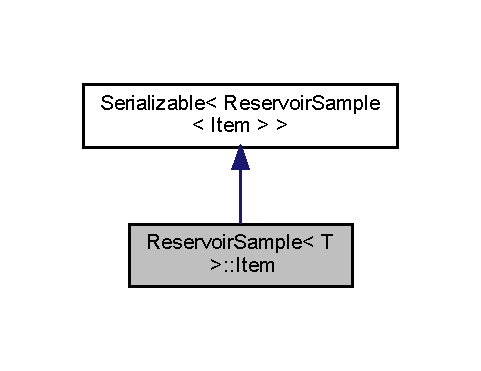
\includegraphics[width=231pt]{struct_reservoir_sample_1_1_item__inherit__graph}
\end{center}
\end{figure}


Collaboration diagram for Reservoir\+Sample$<$ T $>$\+::Item\+:
\nopagebreak
\begin{figure}[H]
\begin{center}
\leavevmode
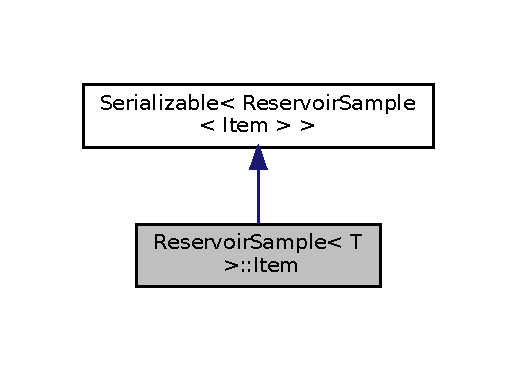
\includegraphics[width=231pt]{struct_reservoir_sample_1_1_item__coll__graph}
\end{center}
\end{figure}
\doxysubsection*{Public Member Functions}
\begin{DoxyCompactItemize}
\item 
\mbox{\hyperlink{struct_reservoir_sample_1_1_item_a01a115a4bc68485d3349d61b85388998}{Item}} (T x\+\_\+, double r\+\_\+)
\item 
bool \mbox{\hyperlink{struct_reservoir_sample_1_1_item_a6021bbb1eaadfab8990b05557e2758fa}{operator$<$}} (const \mbox{\hyperlink{struct_reservoir_sample_1_1_item}{Item}} \&b) const
\item 
bool \mbox{\hyperlink{struct_reservoir_sample_1_1_item_a3acc4a4c4aca6d80629d35f9a37220ff}{operator==}} (const \mbox{\hyperlink{struct_reservoir_sample_1_1_item}{Item}} \&b) const
\item 
void \mbox{\hyperlink{struct_reservoir_sample_1_1_item_aefa79bdf7a5dd70f62a41f6ccb0ac066}{print}} () const
\item 
virtual std\+::string \mbox{\hyperlink{struct_reservoir_sample_1_1_item_a92696114cc5bb287b99c0c3452e0973b}{serialize}} () const override
\end{DoxyCompactItemize}
\doxysubsection*{Static Public Member Functions}
\begin{DoxyCompactItemize}
\item 
static \mbox{\hyperlink{struct_reservoir_sample_1_1_item}{Item}} \mbox{\hyperlink{struct_reservoir_sample_1_1_item_a3dcc7bbd0d5c83522ff039627db44c23}{deserialize}} (const std\+::string \&)
\end{DoxyCompactItemize}
\doxysubsection*{Public Attributes}
\begin{DoxyCompactItemize}
\item 
T \mbox{\hyperlink{struct_reservoir_sample_1_1_item_abc1ea374480d6d86d0466e4683c98337}{x}}
\item 
const double \mbox{\hyperlink{struct_reservoir_sample_1_1_item_ad74b6fb33eb3a534eeb4141c735dfaf5}{r}}
\end{DoxyCompactItemize}


\doxysubsection{Detailed Description}
\subsubsection*{template$<$typename T$>$\newline
class Reservoir\+Sample$<$ T $>$\+::\+Item}

\begin{DoxyAuthor}{Author}
piantado 
\end{DoxyAuthor}
\begin{DoxyDate}{Date}
29/01/20 
\end{DoxyDate}


\doxysubsection{Constructor \& Destructor Documentation}
\mbox{\Hypertarget{struct_reservoir_sample_1_1_item_a01a115a4bc68485d3349d61b85388998}\label{struct_reservoir_sample_1_1_item_a01a115a4bc68485d3349d61b85388998}} 
\index{ReservoirSample$<$ T $>$::Item@{ReservoirSample$<$ T $>$::Item}!Item@{Item}}
\index{Item@{Item}!ReservoirSample$<$ T $>$::Item@{ReservoirSample$<$ T $>$::Item}}
\doxysubsubsection{\texorpdfstring{Item()}{Item()}}
{\footnotesize\ttfamily template$<$typename T $>$ \\
\mbox{\hyperlink{class_reservoir_sample}{Reservoir\+Sample}}$<$ T $>$\+::Item\+::\+Item (\begin{DoxyParamCaption}\item[{T}]{x\+\_\+,  }\item[{double}]{r\+\_\+ }\end{DoxyParamCaption})\hspace{0.3cm}{\ttfamily [inline]}}



\doxysubsection{Member Function Documentation}
\mbox{\Hypertarget{struct_reservoir_sample_1_1_item_a3dcc7bbd0d5c83522ff039627db44c23}\label{struct_reservoir_sample_1_1_item_a3dcc7bbd0d5c83522ff039627db44c23}} 
\index{ReservoirSample$<$ T $>$::Item@{ReservoirSample$<$ T $>$::Item}!deserialize@{deserialize}}
\index{deserialize@{deserialize}!ReservoirSample$<$ T $>$::Item@{ReservoirSample$<$ T $>$::Item}}
\doxysubsubsection{\texorpdfstring{deserialize()}{deserialize()}}
{\footnotesize\ttfamily template$<$typename T $>$ \\
static \mbox{\hyperlink{struct_reservoir_sample_1_1_item}{Item}} \mbox{\hyperlink{class_reservoir_sample}{Reservoir\+Sample}}$<$ T $>$\+::Item\+::deserialize (\begin{DoxyParamCaption}\item[{const std\+::string \&}]{ }\end{DoxyParamCaption})\hspace{0.3cm}{\ttfamily [inline]}, {\ttfamily [static]}}

\mbox{\Hypertarget{struct_reservoir_sample_1_1_item_a6021bbb1eaadfab8990b05557e2758fa}\label{struct_reservoir_sample_1_1_item_a6021bbb1eaadfab8990b05557e2758fa}} 
\index{ReservoirSample$<$ T $>$::Item@{ReservoirSample$<$ T $>$::Item}!operator$<$@{operator$<$}}
\index{operator$<$@{operator$<$}!ReservoirSample$<$ T $>$::Item@{ReservoirSample$<$ T $>$::Item}}
\doxysubsubsection{\texorpdfstring{operator$<$()}{operator<()}}
{\footnotesize\ttfamily template$<$typename T $>$ \\
bool \mbox{\hyperlink{class_reservoir_sample}{Reservoir\+Sample}}$<$ T $>$\+::Item\+::operator$<$ (\begin{DoxyParamCaption}\item[{const \mbox{\hyperlink{struct_reservoir_sample_1_1_item}{Item}} \&}]{b }\end{DoxyParamCaption}) const\hspace{0.3cm}{\ttfamily [inline]}}

\mbox{\Hypertarget{struct_reservoir_sample_1_1_item_a3acc4a4c4aca6d80629d35f9a37220ff}\label{struct_reservoir_sample_1_1_item_a3acc4a4c4aca6d80629d35f9a37220ff}} 
\index{ReservoirSample$<$ T $>$::Item@{ReservoirSample$<$ T $>$::Item}!operator==@{operator==}}
\index{operator==@{operator==}!ReservoirSample$<$ T $>$::Item@{ReservoirSample$<$ T $>$::Item}}
\doxysubsubsection{\texorpdfstring{operator==()}{operator==()}}
{\footnotesize\ttfamily template$<$typename T $>$ \\
bool \mbox{\hyperlink{class_reservoir_sample}{Reservoir\+Sample}}$<$ T $>$\+::Item\+::operator== (\begin{DoxyParamCaption}\item[{const \mbox{\hyperlink{struct_reservoir_sample_1_1_item}{Item}} \&}]{b }\end{DoxyParamCaption}) const\hspace{0.3cm}{\ttfamily [inline]}}

\mbox{\Hypertarget{struct_reservoir_sample_1_1_item_aefa79bdf7a5dd70f62a41f6ccb0ac066}\label{struct_reservoir_sample_1_1_item_aefa79bdf7a5dd70f62a41f6ccb0ac066}} 
\index{ReservoirSample$<$ T $>$::Item@{ReservoirSample$<$ T $>$::Item}!print@{print}}
\index{print@{print}!ReservoirSample$<$ T $>$::Item@{ReservoirSample$<$ T $>$::Item}}
\doxysubsubsection{\texorpdfstring{print()}{print()}}
{\footnotesize\ttfamily template$<$typename T $>$ \\
void \mbox{\hyperlink{class_reservoir_sample}{Reservoir\+Sample}}$<$ T $>$\+::Item\+::print (\begin{DoxyParamCaption}{ }\end{DoxyParamCaption}) const\hspace{0.3cm}{\ttfamily [inline]}}

\mbox{\Hypertarget{struct_reservoir_sample_1_1_item_a92696114cc5bb287b99c0c3452e0973b}\label{struct_reservoir_sample_1_1_item_a92696114cc5bb287b99c0c3452e0973b}} 
\index{ReservoirSample$<$ T $>$::Item@{ReservoirSample$<$ T $>$::Item}!serialize@{serialize}}
\index{serialize@{serialize}!ReservoirSample$<$ T $>$::Item@{ReservoirSample$<$ T $>$::Item}}
\doxysubsubsection{\texorpdfstring{serialize()}{serialize()}}
{\footnotesize\ttfamily template$<$typename T $>$ \\
virtual std\+::string \mbox{\hyperlink{class_reservoir_sample}{Reservoir\+Sample}}$<$ T $>$\+::Item\+::serialize (\begin{DoxyParamCaption}{ }\end{DoxyParamCaption}) const\hspace{0.3cm}{\ttfamily [inline]}, {\ttfamily [override]}, {\ttfamily [virtual]}}



\doxysubsection{Member Data Documentation}
\mbox{\Hypertarget{struct_reservoir_sample_1_1_item_ad74b6fb33eb3a534eeb4141c735dfaf5}\label{struct_reservoir_sample_1_1_item_ad74b6fb33eb3a534eeb4141c735dfaf5}} 
\index{ReservoirSample$<$ T $>$::Item@{ReservoirSample$<$ T $>$::Item}!r@{r}}
\index{r@{r}!ReservoirSample$<$ T $>$::Item@{ReservoirSample$<$ T $>$::Item}}
\doxysubsubsection{\texorpdfstring{r}{r}}
{\footnotesize\ttfamily template$<$typename T $>$ \\
const double \mbox{\hyperlink{class_reservoir_sample}{Reservoir\+Sample}}$<$ T $>$\+::Item\+::r}

\mbox{\Hypertarget{struct_reservoir_sample_1_1_item_abc1ea374480d6d86d0466e4683c98337}\label{struct_reservoir_sample_1_1_item_abc1ea374480d6d86d0466e4683c98337}} 
\index{ReservoirSample$<$ T $>$::Item@{ReservoirSample$<$ T $>$::Item}!x@{x}}
\index{x@{x}!ReservoirSample$<$ T $>$::Item@{ReservoirSample$<$ T $>$::Item}}
\doxysubsubsection{\texorpdfstring{x}{x}}
{\footnotesize\ttfamily template$<$typename T $>$ \\
T \mbox{\hyperlink{class_reservoir_sample}{Reservoir\+Sample}}$<$ T $>$\+::Item\+::x}



The documentation for this class was generated from the following file\+:\begin{DoxyCompactItemize}
\item 
src/\+Statistics/\mbox{\hyperlink{_reservoir_sample_8h}{Reservoir\+Sample.\+h}}\end{DoxyCompactItemize}

\hypertarget{class_combinators_1_1_lazy_normal_forms}{}\section{Combinators\+:\+:Lazy\+Normal\+Forms Class Reference}
\label{class_combinators_1_1_lazy_normal_forms}\index{Combinators\+::\+Lazy\+Normal\+Forms@{Combinators\+::\+Lazy\+Normal\+Forms}}


{\ttfamily \#include $<$Combinators.\+h$>$}



Collaboration diagram for Combinators\+:\+:Lazy\+Normal\+Forms\+:
\nopagebreak
\begin{figure}[H]
\begin{center}
\leavevmode
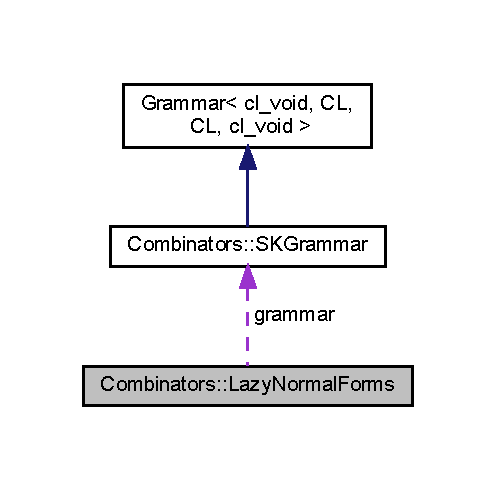
\includegraphics[width=238pt]{class_combinators_1_1_lazy_normal_forms__coll__graph}
\end{center}
\end{figure}
\subsection*{Public Member Functions}
\begin{DoxyCompactItemize}
\item 
\hyperlink{class_combinators_1_1_lazy_normal_forms_ab3e10fd3a3d3611aaffbd11e6e6dd6f0}{Lazy\+Normal\+Forms} (\hyperlink{class_combinators_1_1_s_k_grammar}{S\+K\+Grammar} $\ast$g=\&\hyperlink{namespace_combinators_a24aeacfa083d06000a89cb59d14eeccb}{skgrammar})
\item 
\hyperlink{class_node}{Node} \& \hyperlink{class_combinators_1_1_lazy_normal_forms_a6cd27fdb59899d435c5114288b614067}{at} (const size\+\_\+t i)
\item 
\hyperlink{class_node}{Node} \& \hyperlink{class_combinators_1_1_lazy_normal_forms_a7a95278f40ba41d7148be0d55d46baa4}{next} ()
\end{DoxyCompactItemize}
\subsection*{Public Attributes}
\begin{DoxyCompactItemize}
\item 
size\+\_\+t \hyperlink{class_combinators_1_1_lazy_normal_forms_aad988f6c06e3e1cf4e516ecfc1198c7f}{idx}
\item 
std\+::vector$<$ \hyperlink{class_node}{Node} $>$ \hyperlink{class_combinators_1_1_lazy_normal_forms_aad1e727e4cdf1e6d85c79359698a756b}{list}
\item 
\hyperlink{class_combinators_1_1_s_k_grammar}{S\+K\+Grammar} $\ast$ \hyperlink{class_combinators_1_1_lazy_normal_forms_a67c0d60548475faac5485302174030e2}{grammar}
\end{DoxyCompactItemize}


\subsection{Detailed Description}
\begin{DoxyAuthor}{Author}
piantado 
\end{DoxyAuthor}
\begin{DoxyDate}{Date}
29/04/20 
\end{DoxyDate}


\subsection{Constructor \& Destructor Documentation}
\mbox{\Hypertarget{class_combinators_1_1_lazy_normal_forms_ab3e10fd3a3d3611aaffbd11e6e6dd6f0}\label{class_combinators_1_1_lazy_normal_forms_ab3e10fd3a3d3611aaffbd11e6e6dd6f0}} 
\index{Combinators\+::\+Lazy\+Normal\+Forms@{Combinators\+::\+Lazy\+Normal\+Forms}!Lazy\+Normal\+Forms@{Lazy\+Normal\+Forms}}
\index{Lazy\+Normal\+Forms@{Lazy\+Normal\+Forms}!Combinators\+::\+Lazy\+Normal\+Forms@{Combinators\+::\+Lazy\+Normal\+Forms}}
\subsubsection{\texorpdfstring{Lazy\+Normal\+Forms()}{LazyNormalForms()}}
{\footnotesize\ttfamily Combinators\+::\+Lazy\+Normal\+Forms\+::\+Lazy\+Normal\+Forms (\begin{DoxyParamCaption}\item[{\hyperlink{class_combinators_1_1_s_k_grammar}{S\+K\+Grammar} $\ast$}]{g = {\ttfamily \&\hyperlink{namespace_combinators_a24aeacfa083d06000a89cb59d14eeccb}{skgrammar}} }\end{DoxyParamCaption})\hspace{0.3cm}{\ttfamily [inline]}}



\subsection{Member Function Documentation}
\mbox{\Hypertarget{class_combinators_1_1_lazy_normal_forms_a6cd27fdb59899d435c5114288b614067}\label{class_combinators_1_1_lazy_normal_forms_a6cd27fdb59899d435c5114288b614067}} 
\index{Combinators\+::\+Lazy\+Normal\+Forms@{Combinators\+::\+Lazy\+Normal\+Forms}!at@{at}}
\index{at@{at}!Combinators\+::\+Lazy\+Normal\+Forms@{Combinators\+::\+Lazy\+Normal\+Forms}}
\subsubsection{\texorpdfstring{at()}{at()}}
{\footnotesize\ttfamily \hyperlink{class_node}{Node}\& Combinators\+::\+Lazy\+Normal\+Forms\+::at (\begin{DoxyParamCaption}\item[{const size\+\_\+t}]{i }\end{DoxyParamCaption})\hspace{0.3cm}{\ttfamily [inline]}}

\mbox{\Hypertarget{class_combinators_1_1_lazy_normal_forms_a7a95278f40ba41d7148be0d55d46baa4}\label{class_combinators_1_1_lazy_normal_forms_a7a95278f40ba41d7148be0d55d46baa4}} 
\index{Combinators\+::\+Lazy\+Normal\+Forms@{Combinators\+::\+Lazy\+Normal\+Forms}!next@{next}}
\index{next@{next}!Combinators\+::\+Lazy\+Normal\+Forms@{Combinators\+::\+Lazy\+Normal\+Forms}}
\subsubsection{\texorpdfstring{next()}{next()}}
{\footnotesize\ttfamily \hyperlink{class_node}{Node}\& Combinators\+::\+Lazy\+Normal\+Forms\+::next (\begin{DoxyParamCaption}{ }\end{DoxyParamCaption})\hspace{0.3cm}{\ttfamily [inline]}}



\subsection{Member Data Documentation}
\mbox{\Hypertarget{class_combinators_1_1_lazy_normal_forms_a67c0d60548475faac5485302174030e2}\label{class_combinators_1_1_lazy_normal_forms_a67c0d60548475faac5485302174030e2}} 
\index{Combinators\+::\+Lazy\+Normal\+Forms@{Combinators\+::\+Lazy\+Normal\+Forms}!grammar@{grammar}}
\index{grammar@{grammar}!Combinators\+::\+Lazy\+Normal\+Forms@{Combinators\+::\+Lazy\+Normal\+Forms}}
\subsubsection{\texorpdfstring{grammar}{grammar}}
{\footnotesize\ttfamily \hyperlink{class_combinators_1_1_s_k_grammar}{S\+K\+Grammar}$\ast$ Combinators\+::\+Lazy\+Normal\+Forms\+::grammar}

\mbox{\Hypertarget{class_combinators_1_1_lazy_normal_forms_aad988f6c06e3e1cf4e516ecfc1198c7f}\label{class_combinators_1_1_lazy_normal_forms_aad988f6c06e3e1cf4e516ecfc1198c7f}} 
\index{Combinators\+::\+Lazy\+Normal\+Forms@{Combinators\+::\+Lazy\+Normal\+Forms}!idx@{idx}}
\index{idx@{idx}!Combinators\+::\+Lazy\+Normal\+Forms@{Combinators\+::\+Lazy\+Normal\+Forms}}
\subsubsection{\texorpdfstring{idx}{idx}}
{\footnotesize\ttfamily size\+\_\+t Combinators\+::\+Lazy\+Normal\+Forms\+::idx}

\mbox{\Hypertarget{class_combinators_1_1_lazy_normal_forms_aad1e727e4cdf1e6d85c79359698a756b}\label{class_combinators_1_1_lazy_normal_forms_aad1e727e4cdf1e6d85c79359698a756b}} 
\index{Combinators\+::\+Lazy\+Normal\+Forms@{Combinators\+::\+Lazy\+Normal\+Forms}!list@{list}}
\index{list@{list}!Combinators\+::\+Lazy\+Normal\+Forms@{Combinators\+::\+Lazy\+Normal\+Forms}}
\subsubsection{\texorpdfstring{list}{list}}
{\footnotesize\ttfamily std\+::vector$<$\hyperlink{class_node}{Node}$>$ Combinators\+::\+Lazy\+Normal\+Forms\+::list}



The documentation for this class was generated from the following file\+:\begin{DoxyCompactItemize}
\item 
src/\hyperlink{_combinators_8h}{Combinators.\+h}\end{DoxyCompactItemize}

\hypertarget{class_lexicon}{}\doxysection{Lexicon$<$ this\+\_\+t, key\+\_\+t, I\+N\+N\+ER, \+\_\+input\+\_\+t, \+\_\+output\+\_\+t, datum\+\_\+t, \+\_\+\+Virtual\+Machine\+State\+\_\+t $>$ Class Template Reference}
\label{class_lexicon}\index{Lexicon$<$ this\_t, key\_t, INNER, \_input\_t, \_output\_t, datum\_t, \_VirtualMachineState\_t $>$@{Lexicon$<$ this\_t, key\_t, INNER, \_input\_t, \_output\_t, datum\_t, \_VirtualMachineState\_t $>$}}


{\ttfamily \#include $<$Lexicon.\+h$>$}



Inheritance diagram for Lexicon$<$ this\+\_\+t, key\+\_\+t, I\+N\+N\+ER, \+\_\+input\+\_\+t, \+\_\+output\+\_\+t, datum\+\_\+t, \+\_\+\+Virtual\+Machine\+State\+\_\+t $>$\+:
\nopagebreak
\begin{figure}[H]
\begin{center}
\leavevmode
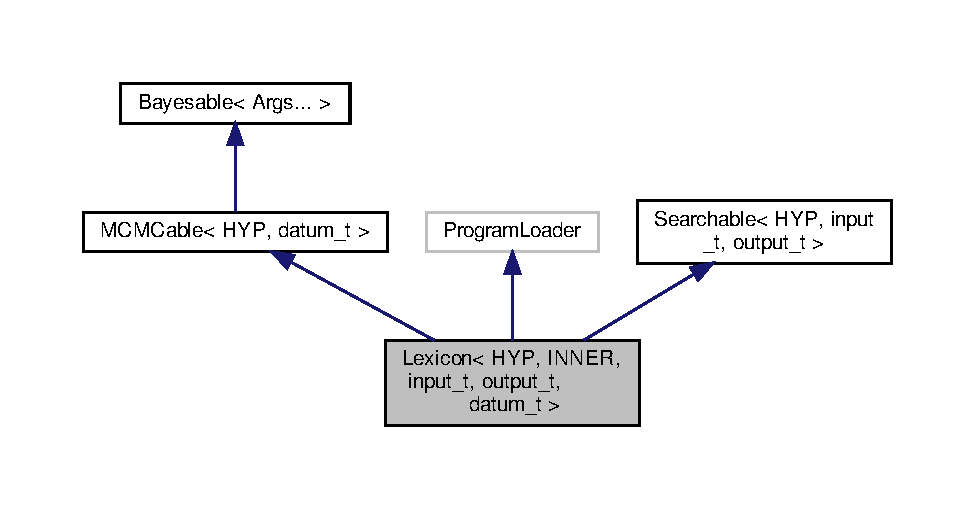
\includegraphics[width=350pt]{class_lexicon__inherit__graph}
\end{center}
\end{figure}


Collaboration diagram for Lexicon$<$ this\+\_\+t, key\+\_\+t, I\+N\+N\+ER, \+\_\+input\+\_\+t, \+\_\+output\+\_\+t, datum\+\_\+t, \+\_\+\+Virtual\+Machine\+State\+\_\+t $>$\+:
\nopagebreak
\begin{figure}[H]
\begin{center}
\leavevmode
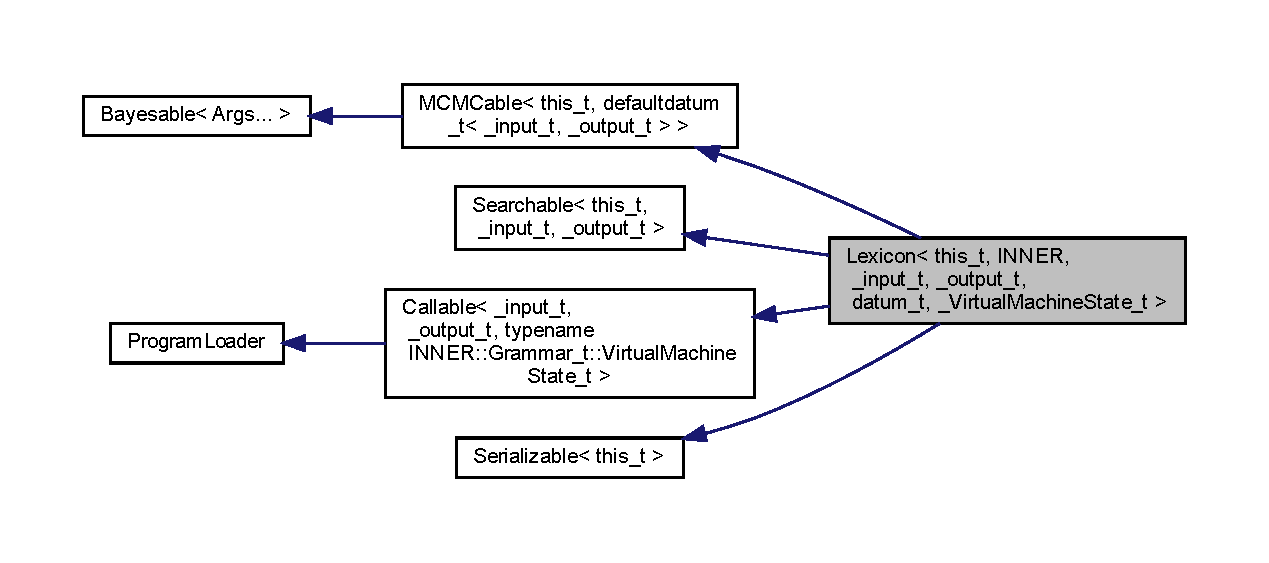
\includegraphics[width=350pt]{class_lexicon__coll__graph}
\end{center}
\end{figure}
\doxysubsection*{Public Types}
\begin{DoxyCompactItemize}
\item 
using \mbox{\hyperlink{class_lexicon_ad31914cd93f183a0a44867682f83e2ba}{Grammar\+\_\+t}} = typename I\+N\+N\+E\+R\+::\+Grammar\+\_\+t
\item 
using \mbox{\hyperlink{class_lexicon_ab33b798113eab99e91ec863e628cf28e}{input\+\_\+t}} = \+\_\+input\+\_\+t
\item 
using \mbox{\hyperlink{class_lexicon_af1f548f77ea928618921f940439e9c18}{output\+\_\+t}} = \+\_\+output\+\_\+t
\item 
using \mbox{\hyperlink{class_lexicon_a37916cf677e3d9f3fe097453f27edb58}{Virtual\+Machine\+State\+\_\+t}} = \+\_\+\+Virtual\+Machine\+State\+\_\+t
\end{DoxyCompactItemize}
\doxysubsection*{Public Member Functions}
\begin{DoxyCompactItemize}
\item 
\mbox{\hyperlink{class_lexicon_a624020980ef4678f083b4c7711880bdf}{Lexicon}} ()
\item 
size\+\_\+t \mbox{\hyperlink{class_lexicon_a6f746ae8e3c2d1111500362393b1fe34}{nfactors}} () const
\begin{DoxyCompactList}\small\item\em Return the number of factors. \end{DoxyCompactList}\item 
auto \& \mbox{\hyperlink{class_lexicon_a10400e633590c75175f9c2e44bbafb41}{get\+\_\+value}} ()
\item 
const auto \& \mbox{\hyperlink{class_lexicon_a2e49c52f34be839fc518b22acf019c32}{get\+\_\+value}} () const
\item 
I\+N\+N\+ER \& \mbox{\hyperlink{class_lexicon_a228ae238863c79bcced14891898ed44e}{at}} (const key\+\_\+t \&k)
\item 
const I\+N\+N\+ER \& \mbox{\hyperlink{class_lexicon_ac2bac014a3eba80beb1a76e1170bd9f7}{at}} (const key\+\_\+t \&k) const
\item 
I\+N\+N\+ER \& \mbox{\hyperlink{class_lexicon_a70707b3449c11f3ac5461e69b9e0a9df}{operator\mbox{[}$\,$\mbox{]}}} (const key\+\_\+t \&k)
\item 
const I\+N\+N\+ER \& \mbox{\hyperlink{class_lexicon_a3ca1e88c235d78dde6590cebf4eae226}{operator\mbox{[}$\,$\mbox{]}}} (const key\+\_\+t \&k) const
\item 
\mbox{\hyperlink{class_lexicon_ad31914cd93f183a0a44867682f83e2ba}{Grammar\+\_\+t}} $\ast$ \mbox{\hyperlink{class_lexicon_acb2a498568a5078985369285214aab0a}{get\+\_\+grammar}} ()
\item 
virtual std\+::string \mbox{\hyperlink{class_lexicon_a90b7fbb8f47821de444910d1c5348a66}{string}} (std\+::string prefix=\char`\"{}\char`\"{}) const override
\item 
virtual size\+\_\+t \mbox{\hyperlink{class_lexicon_a7bdb1eb6e4290e2528a50ef2d2d768b8}{hash}} () const override
\item 
virtual bool \mbox{\hyperlink{class_lexicon_a7623a6f5ad5156789088e461dbe9d2f6}{operator==}} (const this\+\_\+t \&l) const override
\begin{DoxyCompactList}\small\item\em Equality checks equality on each part. \end{DoxyCompactList}\item 
virtual void \mbox{\hyperlink{class_lexicon_a996469fca2205a7cfc086d16992f6362}{push\+\_\+program}} (\mbox{\hyperlink{class_program}{Program}}$<$ \mbox{\hyperlink{class_lexicon_a37916cf677e3d9f3fe097453f27edb58}{Virtual\+Machine\+State\+\_\+t}} $>$ \&s, const key\+\_\+t k) override
\begin{DoxyCompactList}\small\item\em Dispatch key k -- push its program onto the stack. \end{DoxyCompactList}\item 
virtual void \mbox{\hyperlink{class_lexicon_a970ca24ab5c6ae8065809e820861162d}{complete}} () override
\begin{DoxyCompactList}\small\item\em Fill in all the holes in this hypothesis, at random, modifying self. N\+O\+TE for L\+O\+T\+Hypotheses this will also compile, which is what we need to do for a \mbox{\hyperlink{class_l_o_t_hypothesis}{L\+O\+T\+Hypothesis}}. \end{DoxyCompactList}\item 
virtual double \mbox{\hyperlink{class_lexicon_a82e06fa6c6a0892ed6de3694f5abc1b5}{compute\+\_\+prior}} () override
\begin{DoxyCompactList}\small\item\em Compute the prior -- defaultly not defined. \end{DoxyCompactList}\item 
virtual std\+::optional$<$ std\+::pair$<$ this\+\_\+t, double $>$ $>$ \mbox{\hyperlink{class_lexicon_a5de4f2940877e8b55305c1400e540eca}{propose}} () const override
\begin{DoxyCompactList}\small\item\em This proposal guarantees that there will be at least one factor that is proposed to. Each individual factor is proposed to with p\+\_\+factor\+\_\+propose. \end{DoxyCompactList}\item 
virtual this\+\_\+t \mbox{\hyperlink{class_lexicon_a85ac08b4f9c4483f460f845ac80318af}{restart}} () const override
\item 
int \mbox{\hyperlink{class_lexicon_ab55f0b404f7f27abaa75818f6e7fc995}{neighbors}} () const override
\item 
void \mbox{\hyperlink{class_lexicon_a2ad5beab39c33f93990f3fd96a7c137d}{expand\+\_\+to\+\_\+neighbor}} (int k) override
\begin{DoxyCompactList}\small\item\em Modify this hypothesis to become the k\textquotesingle{}th neighbor. N\+O\+TE This does not compile since it might not be complete. \end{DoxyCompactList}\item 
virtual double \mbox{\hyperlink{class_lexicon_a045bf5553a5dcb41584445c6b3ba8338}{neighbor\+\_\+prior}} (int k) override
\begin{DoxyCompactList}\small\item\em What is the prior of the k\textquotesingle{}th neighbor? This does not need to return the full prior, only relative (among ks) \end{DoxyCompactList}\item 
bool \mbox{\hyperlink{class_lexicon_a7f9e969dbfd431bf733a6fb9659c40d3}{is\+\_\+evaluable}} () const override
\item 
virtual \mbox{\hyperlink{class_discrete_distribution}{Discrete\+Distribution}}$<$ \mbox{\hyperlink{class_lexicon_af1f548f77ea928618921f940439e9c18}{output\+\_\+t}} $>$ \mbox{\hyperlink{class_lexicon_a06b3a524733df90ba00f8a9ab5408b61}{call}} (const key\+\_\+t k, const \mbox{\hyperlink{class_lexicon_ab33b798113eab99e91ec863e628cf28e}{input\+\_\+t}} x, const \mbox{\hyperlink{class_lexicon_af1f548f77ea928618921f940439e9c18}{output\+\_\+t}} \&err=\mbox{\hyperlink{class_lexicon_af1f548f77ea928618921f940439e9c18}{output\+\_\+t}}\{\})
\item 
virtual std\+::string \mbox{\hyperlink{class_lexicon_a9cc0c92e5ed9e16f35627806452d102b}{serialize}} () const override
\end{DoxyCompactItemize}
\doxysubsection*{Static Public Member Functions}
\begin{DoxyCompactItemize}
\item 
static this\+\_\+t \mbox{\hyperlink{class_lexicon_ae2154b9ad23fa6ad2e844bdf4ffb00d9}{sample}} (std\+::initializer\+\_\+list$<$ key\+\_\+t $>$ lst)
\begin{DoxyCompactList}\small\item\em Sample with n factors. \end{DoxyCompactList}\item 
{\footnotesize template$<$typename... A$>$ }\\static this\+\_\+t \mbox{\hyperlink{class_lexicon_a0b08b7f7f30a5292b2f11d2f17f2f600}{make}} (A... a)
\item 
static this\+\_\+t \mbox{\hyperlink{class_lexicon_a09d2a0eaf8daa03bd2616c224a0178b6}{deserialize}} (const std\+::string s)
\end{DoxyCompactItemize}
\doxysubsection*{Public Attributes}
\begin{DoxyCompactItemize}
\item 
std\+::map$<$ key\+\_\+t, I\+N\+N\+ER $>$ \mbox{\hyperlink{class_lexicon_aa73021310bd54abc022db58dac9dff48}{factors}}
\end{DoxyCompactItemize}
\doxysubsection*{Static Public Attributes}
\begin{DoxyCompactItemize}
\item 
const static char \mbox{\hyperlink{class_lexicon_ab786b4d297d3f6629f2be6a6f65ec131}{Factor\+Delimiter}} = \textquotesingle{}$\vert$\textquotesingle{}
\item 
static double \mbox{\hyperlink{class_lexicon_a6c45c5f96c1632c10c58e4b71fcf7059}{p\+\_\+factor\+\_\+propose}} = 0.\+5
\end{DoxyCompactItemize}


\doxysubsection{Detailed Description}
\subsubsection*{template$<$typename this\+\_\+t, typename key\+\_\+t, typename I\+N\+N\+ER, typename \+\_\+input\+\_\+t, typename \+\_\+output\+\_\+t, typename datum\+\_\+t = defaultdatum\+\_\+t$<$\+\_\+input\+\_\+t, \+\_\+output\+\_\+t$>$, typename \+\_\+\+Virtual\+Machine\+State\+\_\+t = typename I\+N\+N\+E\+R\+::\+Grammar\+\_\+t\+::\+Virtual\+Machine\+State\+\_\+t$>$\newline
class Lexicon$<$ this\+\_\+t, key\+\_\+t, I\+N\+N\+E\+R, \+\_\+input\+\_\+t, \+\_\+output\+\_\+t, datum\+\_\+t, \+\_\+\+Virtual\+Machine\+State\+\_\+t $>$}

\begin{DoxyAuthor}{Author}
piantado 
\end{DoxyAuthor}
\begin{DoxyDate}{Date}
29/01/20 
\end{DoxyDate}


\doxysubsection{Member Typedef Documentation}
\mbox{\Hypertarget{class_lexicon_ad31914cd93f183a0a44867682f83e2ba}\label{class_lexicon_ad31914cd93f183a0a44867682f83e2ba}} 
\index{Lexicon$<$ this\_t, key\_t, INNER, \_input\_t, \_output\_t, datum\_t, \_VirtualMachineState\_t $>$@{Lexicon$<$ this\_t, key\_t, INNER, \_input\_t, \_output\_t, datum\_t, \_VirtualMachineState\_t $>$}!Grammar\_t@{Grammar\_t}}
\index{Grammar\_t@{Grammar\_t}!Lexicon$<$ this\_t, key\_t, INNER, \_input\_t, \_output\_t, datum\_t, \_VirtualMachineState\_t $>$@{Lexicon$<$ this\_t, key\_t, INNER, \_input\_t, \_output\_t, datum\_t, \_VirtualMachineState\_t $>$}}
\doxysubsubsection{\texorpdfstring{Grammar\_t}{Grammar\_t}}
{\footnotesize\ttfamily template$<$typename this\+\_\+t , typename key\+\_\+t , typename I\+N\+N\+ER , typename \+\_\+input\+\_\+t , typename \+\_\+output\+\_\+t , typename datum\+\_\+t  = defaultdatum\+\_\+t$<$\+\_\+input\+\_\+t, \+\_\+output\+\_\+t$>$, typename \+\_\+\+Virtual\+Machine\+State\+\_\+t  = typename I\+N\+N\+E\+R\+::\+Grammar\+\_\+t\+::\+Virtual\+Machine\+State\+\_\+t$>$ \\
using \mbox{\hyperlink{class_lexicon}{Lexicon}}$<$ this\+\_\+t, key\+\_\+t, I\+N\+N\+ER, \+\_\+input\+\_\+t, \+\_\+output\+\_\+t, \mbox{\hyperlink{class_bayesable_a9f1a6c0cd7855550fa10b1a8f13a5867}{datum\+\_\+t}}, \+\_\+\+Virtual\+Machine\+State\+\_\+t $>$\+::\mbox{\hyperlink{class_lexicon_ad31914cd93f183a0a44867682f83e2ba}{Grammar\+\_\+t}} =  typename I\+N\+N\+E\+R\+::\+Grammar\+\_\+t}

\mbox{\Hypertarget{class_lexicon_ab33b798113eab99e91ec863e628cf28e}\label{class_lexicon_ab33b798113eab99e91ec863e628cf28e}} 
\index{Lexicon$<$ this\_t, key\_t, INNER, \_input\_t, \_output\_t, datum\_t, \_VirtualMachineState\_t $>$@{Lexicon$<$ this\_t, key\_t, INNER, \_input\_t, \_output\_t, datum\_t, \_VirtualMachineState\_t $>$}!input\_t@{input\_t}}
\index{input\_t@{input\_t}!Lexicon$<$ this\_t, key\_t, INNER, \_input\_t, \_output\_t, datum\_t, \_VirtualMachineState\_t $>$@{Lexicon$<$ this\_t, key\_t, INNER, \_input\_t, \_output\_t, datum\_t, \_VirtualMachineState\_t $>$}}
\doxysubsubsection{\texorpdfstring{input\_t}{input\_t}}
{\footnotesize\ttfamily template$<$typename this\+\_\+t , typename key\+\_\+t , typename I\+N\+N\+ER , typename \+\_\+input\+\_\+t , typename \+\_\+output\+\_\+t , typename datum\+\_\+t  = defaultdatum\+\_\+t$<$\+\_\+input\+\_\+t, \+\_\+output\+\_\+t$>$, typename \+\_\+\+Virtual\+Machine\+State\+\_\+t  = typename I\+N\+N\+E\+R\+::\+Grammar\+\_\+t\+::\+Virtual\+Machine\+State\+\_\+t$>$ \\
using \mbox{\hyperlink{class_lexicon}{Lexicon}}$<$ this\+\_\+t, key\+\_\+t, I\+N\+N\+ER, \+\_\+input\+\_\+t, \+\_\+output\+\_\+t, \mbox{\hyperlink{class_bayesable_a9f1a6c0cd7855550fa10b1a8f13a5867}{datum\+\_\+t}}, \+\_\+\+Virtual\+Machine\+State\+\_\+t $>$\+::\mbox{\hyperlink{class_lexicon_ab33b798113eab99e91ec863e628cf28e}{input\+\_\+t}} =  \+\_\+input\+\_\+t}

\mbox{\Hypertarget{class_lexicon_af1f548f77ea928618921f940439e9c18}\label{class_lexicon_af1f548f77ea928618921f940439e9c18}} 
\index{Lexicon$<$ this\_t, key\_t, INNER, \_input\_t, \_output\_t, datum\_t, \_VirtualMachineState\_t $>$@{Lexicon$<$ this\_t, key\_t, INNER, \_input\_t, \_output\_t, datum\_t, \_VirtualMachineState\_t $>$}!output\_t@{output\_t}}
\index{output\_t@{output\_t}!Lexicon$<$ this\_t, key\_t, INNER, \_input\_t, \_output\_t, datum\_t, \_VirtualMachineState\_t $>$@{Lexicon$<$ this\_t, key\_t, INNER, \_input\_t, \_output\_t, datum\_t, \_VirtualMachineState\_t $>$}}
\doxysubsubsection{\texorpdfstring{output\_t}{output\_t}}
{\footnotesize\ttfamily template$<$typename this\+\_\+t , typename key\+\_\+t , typename I\+N\+N\+ER , typename \+\_\+input\+\_\+t , typename \+\_\+output\+\_\+t , typename datum\+\_\+t  = defaultdatum\+\_\+t$<$\+\_\+input\+\_\+t, \+\_\+output\+\_\+t$>$, typename \+\_\+\+Virtual\+Machine\+State\+\_\+t  = typename I\+N\+N\+E\+R\+::\+Grammar\+\_\+t\+::\+Virtual\+Machine\+State\+\_\+t$>$ \\
using \mbox{\hyperlink{class_lexicon}{Lexicon}}$<$ this\+\_\+t, key\+\_\+t, I\+N\+N\+ER, \+\_\+input\+\_\+t, \+\_\+output\+\_\+t, \mbox{\hyperlink{class_bayesable_a9f1a6c0cd7855550fa10b1a8f13a5867}{datum\+\_\+t}}, \+\_\+\+Virtual\+Machine\+State\+\_\+t $>$\+::\mbox{\hyperlink{class_lexicon_af1f548f77ea928618921f940439e9c18}{output\+\_\+t}} =  \+\_\+output\+\_\+t}

\mbox{\Hypertarget{class_lexicon_a37916cf677e3d9f3fe097453f27edb58}\label{class_lexicon_a37916cf677e3d9f3fe097453f27edb58}} 
\index{Lexicon$<$ this\_t, key\_t, INNER, \_input\_t, \_output\_t, datum\_t, \_VirtualMachineState\_t $>$@{Lexicon$<$ this\_t, key\_t, INNER, \_input\_t, \_output\_t, datum\_t, \_VirtualMachineState\_t $>$}!VirtualMachineState\_t@{VirtualMachineState\_t}}
\index{VirtualMachineState\_t@{VirtualMachineState\_t}!Lexicon$<$ this\_t, key\_t, INNER, \_input\_t, \_output\_t, datum\_t, \_VirtualMachineState\_t $>$@{Lexicon$<$ this\_t, key\_t, INNER, \_input\_t, \_output\_t, datum\_t, \_VirtualMachineState\_t $>$}}
\doxysubsubsection{\texorpdfstring{VirtualMachineState\_t}{VirtualMachineState\_t}}
{\footnotesize\ttfamily template$<$typename this\+\_\+t , typename key\+\_\+t , typename I\+N\+N\+ER , typename \+\_\+input\+\_\+t , typename \+\_\+output\+\_\+t , typename datum\+\_\+t  = defaultdatum\+\_\+t$<$\+\_\+input\+\_\+t, \+\_\+output\+\_\+t$>$, typename \+\_\+\+Virtual\+Machine\+State\+\_\+t  = typename I\+N\+N\+E\+R\+::\+Grammar\+\_\+t\+::\+Virtual\+Machine\+State\+\_\+t$>$ \\
using \mbox{\hyperlink{class_lexicon}{Lexicon}}$<$ this\+\_\+t, key\+\_\+t, I\+N\+N\+ER, \+\_\+input\+\_\+t, \+\_\+output\+\_\+t, \mbox{\hyperlink{class_bayesable_a9f1a6c0cd7855550fa10b1a8f13a5867}{datum\+\_\+t}}, \+\_\+\+Virtual\+Machine\+State\+\_\+t $>$\+::\mbox{\hyperlink{class_lexicon_a37916cf677e3d9f3fe097453f27edb58}{Virtual\+Machine\+State\+\_\+t}} =  \+\_\+\+Virtual\+Machine\+State\+\_\+t}



\doxysubsection{Constructor \& Destructor Documentation}
\mbox{\Hypertarget{class_lexicon_a624020980ef4678f083b4c7711880bdf}\label{class_lexicon_a624020980ef4678f083b4c7711880bdf}} 
\index{Lexicon$<$ this\_t, key\_t, INNER, \_input\_t, \_output\_t, datum\_t, \_VirtualMachineState\_t $>$@{Lexicon$<$ this\_t, key\_t, INNER, \_input\_t, \_output\_t, datum\_t, \_VirtualMachineState\_t $>$}!Lexicon@{Lexicon}}
\index{Lexicon@{Lexicon}!Lexicon$<$ this\_t, key\_t, INNER, \_input\_t, \_output\_t, datum\_t, \_VirtualMachineState\_t $>$@{Lexicon$<$ this\_t, key\_t, INNER, \_input\_t, \_output\_t, datum\_t, \_VirtualMachineState\_t $>$}}
\doxysubsubsection{\texorpdfstring{Lexicon()}{Lexicon()}}
{\footnotesize\ttfamily template$<$typename this\+\_\+t , typename key\+\_\+t , typename I\+N\+N\+ER , typename \+\_\+input\+\_\+t , typename \+\_\+output\+\_\+t , typename datum\+\_\+t  = defaultdatum\+\_\+t$<$\+\_\+input\+\_\+t, \+\_\+output\+\_\+t$>$, typename \+\_\+\+Virtual\+Machine\+State\+\_\+t  = typename I\+N\+N\+E\+R\+::\+Grammar\+\_\+t\+::\+Virtual\+Machine\+State\+\_\+t$>$ \\
\mbox{\hyperlink{class_lexicon}{Lexicon}}$<$ this\+\_\+t, key\+\_\+t, I\+N\+N\+ER, \+\_\+input\+\_\+t, \+\_\+output\+\_\+t, \mbox{\hyperlink{class_bayesable_a9f1a6c0cd7855550fa10b1a8f13a5867}{datum\+\_\+t}}, \+\_\+\+Virtual\+Machine\+State\+\_\+t $>$\+::\mbox{\hyperlink{class_lexicon}{Lexicon}} (\begin{DoxyParamCaption}{ }\end{DoxyParamCaption})\hspace{0.3cm}{\ttfamily [inline]}}



\doxysubsection{Member Function Documentation}
\mbox{\Hypertarget{class_lexicon_a228ae238863c79bcced14891898ed44e}\label{class_lexicon_a228ae238863c79bcced14891898ed44e}} 
\index{Lexicon$<$ this\_t, key\_t, INNER, \_input\_t, \_output\_t, datum\_t, \_VirtualMachineState\_t $>$@{Lexicon$<$ this\_t, key\_t, INNER, \_input\_t, \_output\_t, datum\_t, \_VirtualMachineState\_t $>$}!at@{at}}
\index{at@{at}!Lexicon$<$ this\_t, key\_t, INNER, \_input\_t, \_output\_t, datum\_t, \_VirtualMachineState\_t $>$@{Lexicon$<$ this\_t, key\_t, INNER, \_input\_t, \_output\_t, datum\_t, \_VirtualMachineState\_t $>$}}
\doxysubsubsection{\texorpdfstring{at()}{at()}\hspace{0.1cm}{\footnotesize\ttfamily [1/2]}}
{\footnotesize\ttfamily template$<$typename this\+\_\+t , typename key\+\_\+t , typename I\+N\+N\+ER , typename \+\_\+input\+\_\+t , typename \+\_\+output\+\_\+t , typename datum\+\_\+t  = defaultdatum\+\_\+t$<$\+\_\+input\+\_\+t, \+\_\+output\+\_\+t$>$, typename \+\_\+\+Virtual\+Machine\+State\+\_\+t  = typename I\+N\+N\+E\+R\+::\+Grammar\+\_\+t\+::\+Virtual\+Machine\+State\+\_\+t$>$ \\
I\+N\+N\+ER\& \mbox{\hyperlink{class_lexicon}{Lexicon}}$<$ this\+\_\+t, key\+\_\+t, I\+N\+N\+ER, \+\_\+input\+\_\+t, \+\_\+output\+\_\+t, \mbox{\hyperlink{class_bayesable_a9f1a6c0cd7855550fa10b1a8f13a5867}{datum\+\_\+t}}, \+\_\+\+Virtual\+Machine\+State\+\_\+t $>$\+::at (\begin{DoxyParamCaption}\item[{const key\+\_\+t \&}]{k }\end{DoxyParamCaption})\hspace{0.3cm}{\ttfamily [inline]}}

\mbox{\Hypertarget{class_lexicon_ac2bac014a3eba80beb1a76e1170bd9f7}\label{class_lexicon_ac2bac014a3eba80beb1a76e1170bd9f7}} 
\index{Lexicon$<$ this\_t, key\_t, INNER, \_input\_t, \_output\_t, datum\_t, \_VirtualMachineState\_t $>$@{Lexicon$<$ this\_t, key\_t, INNER, \_input\_t, \_output\_t, datum\_t, \_VirtualMachineState\_t $>$}!at@{at}}
\index{at@{at}!Lexicon$<$ this\_t, key\_t, INNER, \_input\_t, \_output\_t, datum\_t, \_VirtualMachineState\_t $>$@{Lexicon$<$ this\_t, key\_t, INNER, \_input\_t, \_output\_t, datum\_t, \_VirtualMachineState\_t $>$}}
\doxysubsubsection{\texorpdfstring{at()}{at()}\hspace{0.1cm}{\footnotesize\ttfamily [2/2]}}
{\footnotesize\ttfamily template$<$typename this\+\_\+t , typename key\+\_\+t , typename I\+N\+N\+ER , typename \+\_\+input\+\_\+t , typename \+\_\+output\+\_\+t , typename datum\+\_\+t  = defaultdatum\+\_\+t$<$\+\_\+input\+\_\+t, \+\_\+output\+\_\+t$>$, typename \+\_\+\+Virtual\+Machine\+State\+\_\+t  = typename I\+N\+N\+E\+R\+::\+Grammar\+\_\+t\+::\+Virtual\+Machine\+State\+\_\+t$>$ \\
const I\+N\+N\+ER\& \mbox{\hyperlink{class_lexicon}{Lexicon}}$<$ this\+\_\+t, key\+\_\+t, I\+N\+N\+ER, \+\_\+input\+\_\+t, \+\_\+output\+\_\+t, \mbox{\hyperlink{class_bayesable_a9f1a6c0cd7855550fa10b1a8f13a5867}{datum\+\_\+t}}, \+\_\+\+Virtual\+Machine\+State\+\_\+t $>$\+::at (\begin{DoxyParamCaption}\item[{const key\+\_\+t \&}]{k }\end{DoxyParamCaption}) const\hspace{0.3cm}{\ttfamily [inline]}}

\mbox{\Hypertarget{class_lexicon_a06b3a524733df90ba00f8a9ab5408b61}\label{class_lexicon_a06b3a524733df90ba00f8a9ab5408b61}} 
\index{Lexicon$<$ this\_t, key\_t, INNER, \_input\_t, \_output\_t, datum\_t, \_VirtualMachineState\_t $>$@{Lexicon$<$ this\_t, key\_t, INNER, \_input\_t, \_output\_t, datum\_t, \_VirtualMachineState\_t $>$}!call@{call}}
\index{call@{call}!Lexicon$<$ this\_t, key\_t, INNER, \_input\_t, \_output\_t, datum\_t, \_VirtualMachineState\_t $>$@{Lexicon$<$ this\_t, key\_t, INNER, \_input\_t, \_output\_t, datum\_t, \_VirtualMachineState\_t $>$}}
\doxysubsubsection{\texorpdfstring{call()}{call()}}
{\footnotesize\ttfamily template$<$typename this\+\_\+t , typename key\+\_\+t , typename I\+N\+N\+ER , typename \+\_\+input\+\_\+t , typename \+\_\+output\+\_\+t , typename datum\+\_\+t  = defaultdatum\+\_\+t$<$\+\_\+input\+\_\+t, \+\_\+output\+\_\+t$>$, typename \+\_\+\+Virtual\+Machine\+State\+\_\+t  = typename I\+N\+N\+E\+R\+::\+Grammar\+\_\+t\+::\+Virtual\+Machine\+State\+\_\+t$>$ \\
virtual \mbox{\hyperlink{class_discrete_distribution}{Discrete\+Distribution}}$<$\mbox{\hyperlink{class_lexicon_af1f548f77ea928618921f940439e9c18}{output\+\_\+t}}$>$ \mbox{\hyperlink{class_lexicon}{Lexicon}}$<$ this\+\_\+t, key\+\_\+t, I\+N\+N\+ER, \+\_\+input\+\_\+t, \+\_\+output\+\_\+t, \mbox{\hyperlink{class_bayesable_a9f1a6c0cd7855550fa10b1a8f13a5867}{datum\+\_\+t}}, \+\_\+\+Virtual\+Machine\+State\+\_\+t $>$\+::call (\begin{DoxyParamCaption}\item[{const key\+\_\+t}]{k,  }\item[{const \mbox{\hyperlink{class_lexicon_ab33b798113eab99e91ec863e628cf28e}{input\+\_\+t}}}]{x,  }\item[{const \mbox{\hyperlink{class_lexicon_af1f548f77ea928618921f940439e9c18}{output\+\_\+t}} \&}]{err = {\ttfamily \mbox{\hyperlink{class_lexicon_af1f548f77ea928618921f940439e9c18}{output\+\_\+t}}\{\}} }\end{DoxyParamCaption})\hspace{0.3cm}{\ttfamily [inline]}, {\ttfamily [virtual]}}

\mbox{\Hypertarget{class_lexicon_a970ca24ab5c6ae8065809e820861162d}\label{class_lexicon_a970ca24ab5c6ae8065809e820861162d}} 
\index{Lexicon$<$ this\_t, key\_t, INNER, \_input\_t, \_output\_t, datum\_t, \_VirtualMachineState\_t $>$@{Lexicon$<$ this\_t, key\_t, INNER, \_input\_t, \_output\_t, datum\_t, \_VirtualMachineState\_t $>$}!complete@{complete}}
\index{complete@{complete}!Lexicon$<$ this\_t, key\_t, INNER, \_input\_t, \_output\_t, datum\_t, \_VirtualMachineState\_t $>$@{Lexicon$<$ this\_t, key\_t, INNER, \_input\_t, \_output\_t, datum\_t, \_VirtualMachineState\_t $>$}}
\doxysubsubsection{\texorpdfstring{complete()}{complete()}}
{\footnotesize\ttfamily template$<$typename this\+\_\+t , typename key\+\_\+t , typename I\+N\+N\+ER , typename \+\_\+input\+\_\+t , typename \+\_\+output\+\_\+t , typename datum\+\_\+t  = defaultdatum\+\_\+t$<$\+\_\+input\+\_\+t, \+\_\+output\+\_\+t$>$, typename \+\_\+\+Virtual\+Machine\+State\+\_\+t  = typename I\+N\+N\+E\+R\+::\+Grammar\+\_\+t\+::\+Virtual\+Machine\+State\+\_\+t$>$ \\
virtual void \mbox{\hyperlink{class_lexicon}{Lexicon}}$<$ this\+\_\+t, key\+\_\+t, I\+N\+N\+ER, \+\_\+input\+\_\+t, \+\_\+output\+\_\+t, \mbox{\hyperlink{class_bayesable_a9f1a6c0cd7855550fa10b1a8f13a5867}{datum\+\_\+t}}, \+\_\+\+Virtual\+Machine\+State\+\_\+t $>$\+::complete (\begin{DoxyParamCaption}{ }\end{DoxyParamCaption})\hspace{0.3cm}{\ttfamily [inline]}, {\ttfamily [override]}, {\ttfamily [virtual]}}



Fill in all the holes in this hypothesis, at random, modifying self. N\+O\+TE for L\+O\+T\+Hypotheses this will also compile, which is what we need to do for a \mbox{\hyperlink{class_l_o_t_hypothesis}{L\+O\+T\+Hypothesis}}. 



Implements \mbox{\hyperlink{class_searchable_a29ab2eb0471e2e9d96d39f0349f21571}{Searchable$<$ this\+\_\+t, \+\_\+input\+\_\+t, \+\_\+output\+\_\+t $>$}}.

\mbox{\Hypertarget{class_lexicon_a82e06fa6c6a0892ed6de3694f5abc1b5}\label{class_lexicon_a82e06fa6c6a0892ed6de3694f5abc1b5}} 
\index{Lexicon$<$ this\_t, key\_t, INNER, \_input\_t, \_output\_t, datum\_t, \_VirtualMachineState\_t $>$@{Lexicon$<$ this\_t, key\_t, INNER, \_input\_t, \_output\_t, datum\_t, \_VirtualMachineState\_t $>$}!compute\_prior@{compute\_prior}}
\index{compute\_prior@{compute\_prior}!Lexicon$<$ this\_t, key\_t, INNER, \_input\_t, \_output\_t, datum\_t, \_VirtualMachineState\_t $>$@{Lexicon$<$ this\_t, key\_t, INNER, \_input\_t, \_output\_t, datum\_t, \_VirtualMachineState\_t $>$}}
\doxysubsubsection{\texorpdfstring{compute\_prior()}{compute\_prior()}}
{\footnotesize\ttfamily template$<$typename this\+\_\+t , typename key\+\_\+t , typename I\+N\+N\+ER , typename \+\_\+input\+\_\+t , typename \+\_\+output\+\_\+t , typename datum\+\_\+t  = defaultdatum\+\_\+t$<$\+\_\+input\+\_\+t, \+\_\+output\+\_\+t$>$, typename \+\_\+\+Virtual\+Machine\+State\+\_\+t  = typename I\+N\+N\+E\+R\+::\+Grammar\+\_\+t\+::\+Virtual\+Machine\+State\+\_\+t$>$ \\
virtual double \mbox{\hyperlink{class_lexicon}{Lexicon}}$<$ this\+\_\+t, key\+\_\+t, I\+N\+N\+ER, \+\_\+input\+\_\+t, \+\_\+output\+\_\+t, \mbox{\hyperlink{class_bayesable_a9f1a6c0cd7855550fa10b1a8f13a5867}{datum\+\_\+t}}, \+\_\+\+Virtual\+Machine\+State\+\_\+t $>$\+::compute\+\_\+prior (\begin{DoxyParamCaption}{ }\end{DoxyParamCaption})\hspace{0.3cm}{\ttfamily [inline]}, {\ttfamily [override]}, {\ttfamily [virtual]}}



Compute the prior -- defaultly not defined. 



Implements \mbox{\hyperlink{class_bayesable_a1b057a17212ced123545133e2297c01b}{Bayesable$<$ Args... $>$}}.

\mbox{\Hypertarget{class_lexicon_a09d2a0eaf8daa03bd2616c224a0178b6}\label{class_lexicon_a09d2a0eaf8daa03bd2616c224a0178b6}} 
\index{Lexicon$<$ this\_t, key\_t, INNER, \_input\_t, \_output\_t, datum\_t, \_VirtualMachineState\_t $>$@{Lexicon$<$ this\_t, key\_t, INNER, \_input\_t, \_output\_t, datum\_t, \_VirtualMachineState\_t $>$}!deserialize@{deserialize}}
\index{deserialize@{deserialize}!Lexicon$<$ this\_t, key\_t, INNER, \_input\_t, \_output\_t, datum\_t, \_VirtualMachineState\_t $>$@{Lexicon$<$ this\_t, key\_t, INNER, \_input\_t, \_output\_t, datum\_t, \_VirtualMachineState\_t $>$}}
\doxysubsubsection{\texorpdfstring{deserialize()}{deserialize()}}
{\footnotesize\ttfamily template$<$typename this\+\_\+t , typename key\+\_\+t , typename I\+N\+N\+ER , typename \+\_\+input\+\_\+t , typename \+\_\+output\+\_\+t , typename datum\+\_\+t  = defaultdatum\+\_\+t$<$\+\_\+input\+\_\+t, \+\_\+output\+\_\+t$>$, typename \+\_\+\+Virtual\+Machine\+State\+\_\+t  = typename I\+N\+N\+E\+R\+::\+Grammar\+\_\+t\+::\+Virtual\+Machine\+State\+\_\+t$>$ \\
static this\+\_\+t \mbox{\hyperlink{class_lexicon}{Lexicon}}$<$ this\+\_\+t, key\+\_\+t, I\+N\+N\+ER, \+\_\+input\+\_\+t, \+\_\+output\+\_\+t, \mbox{\hyperlink{class_bayesable_a9f1a6c0cd7855550fa10b1a8f13a5867}{datum\+\_\+t}}, \+\_\+\+Virtual\+Machine\+State\+\_\+t $>$\+::deserialize (\begin{DoxyParamCaption}\item[{const std\+::string}]{s }\end{DoxyParamCaption})\hspace{0.3cm}{\ttfamily [inline]}, {\ttfamily [static]}}

Convert a string to a lexicon of this type 
\begin{DoxyParams}{Parameters}
{\em g} & \\
\hline
{\em s} & \\
\hline
\end{DoxyParams}
\begin{DoxyReturn}{Returns}

\end{DoxyReturn}
\mbox{\Hypertarget{class_lexicon_a2ad5beab39c33f93990f3fd96a7c137d}\label{class_lexicon_a2ad5beab39c33f93990f3fd96a7c137d}} 
\index{Lexicon$<$ this\_t, key\_t, INNER, \_input\_t, \_output\_t, datum\_t, \_VirtualMachineState\_t $>$@{Lexicon$<$ this\_t, key\_t, INNER, \_input\_t, \_output\_t, datum\_t, \_VirtualMachineState\_t $>$}!expand\_to\_neighbor@{expand\_to\_neighbor}}
\index{expand\_to\_neighbor@{expand\_to\_neighbor}!Lexicon$<$ this\_t, key\_t, INNER, \_input\_t, \_output\_t, datum\_t, \_VirtualMachineState\_t $>$@{Lexicon$<$ this\_t, key\_t, INNER, \_input\_t, \_output\_t, datum\_t, \_VirtualMachineState\_t $>$}}
\doxysubsubsection{\texorpdfstring{expand\_to\_neighbor()}{expand\_to\_neighbor()}}
{\footnotesize\ttfamily template$<$typename this\+\_\+t , typename key\+\_\+t , typename I\+N\+N\+ER , typename \+\_\+input\+\_\+t , typename \+\_\+output\+\_\+t , typename datum\+\_\+t  = defaultdatum\+\_\+t$<$\+\_\+input\+\_\+t, \+\_\+output\+\_\+t$>$, typename \+\_\+\+Virtual\+Machine\+State\+\_\+t  = typename I\+N\+N\+E\+R\+::\+Grammar\+\_\+t\+::\+Virtual\+Machine\+State\+\_\+t$>$ \\
void \mbox{\hyperlink{class_lexicon}{Lexicon}}$<$ this\+\_\+t, key\+\_\+t, I\+N\+N\+ER, \+\_\+input\+\_\+t, \+\_\+output\+\_\+t, \mbox{\hyperlink{class_bayesable_a9f1a6c0cd7855550fa10b1a8f13a5867}{datum\+\_\+t}}, \+\_\+\+Virtual\+Machine\+State\+\_\+t $>$\+::expand\+\_\+to\+\_\+neighbor (\begin{DoxyParamCaption}\item[{int}]{k }\end{DoxyParamCaption})\hspace{0.3cm}{\ttfamily [inline]}, {\ttfamily [override]}, {\ttfamily [virtual]}}



Modify this hypothesis to become the k\textquotesingle{}th neighbor. N\+O\+TE This does not compile since it might not be complete. 


\begin{DoxyParams}{Parameters}
{\em k} & \\
\hline
\end{DoxyParams}


Implements \mbox{\hyperlink{class_searchable_a9088dba3920f4c66ce671aa16a7d29a4}{Searchable$<$ this\+\_\+t, \+\_\+input\+\_\+t, \+\_\+output\+\_\+t $>$}}.

\mbox{\Hypertarget{class_lexicon_acb2a498568a5078985369285214aab0a}\label{class_lexicon_acb2a498568a5078985369285214aab0a}} 
\index{Lexicon$<$ this\_t, key\_t, INNER, \_input\_t, \_output\_t, datum\_t, \_VirtualMachineState\_t $>$@{Lexicon$<$ this\_t, key\_t, INNER, \_input\_t, \_output\_t, datum\_t, \_VirtualMachineState\_t $>$}!get\_grammar@{get\_grammar}}
\index{get\_grammar@{get\_grammar}!Lexicon$<$ this\_t, key\_t, INNER, \_input\_t, \_output\_t, datum\_t, \_VirtualMachineState\_t $>$@{Lexicon$<$ this\_t, key\_t, INNER, \_input\_t, \_output\_t, datum\_t, \_VirtualMachineState\_t $>$}}
\doxysubsubsection{\texorpdfstring{get\_grammar()}{get\_grammar()}}
{\footnotesize\ttfamily template$<$typename this\+\_\+t , typename key\+\_\+t , typename I\+N\+N\+ER , typename \+\_\+input\+\_\+t , typename \+\_\+output\+\_\+t , typename datum\+\_\+t  = defaultdatum\+\_\+t$<$\+\_\+input\+\_\+t, \+\_\+output\+\_\+t$>$, typename \+\_\+\+Virtual\+Machine\+State\+\_\+t  = typename I\+N\+N\+E\+R\+::\+Grammar\+\_\+t\+::\+Virtual\+Machine\+State\+\_\+t$>$ \\
\mbox{\hyperlink{class_lexicon_ad31914cd93f183a0a44867682f83e2ba}{Grammar\+\_\+t}}$\ast$ \mbox{\hyperlink{class_lexicon}{Lexicon}}$<$ this\+\_\+t, key\+\_\+t, I\+N\+N\+ER, \+\_\+input\+\_\+t, \+\_\+output\+\_\+t, \mbox{\hyperlink{class_bayesable_a9f1a6c0cd7855550fa10b1a8f13a5867}{datum\+\_\+t}}, \+\_\+\+Virtual\+Machine\+State\+\_\+t $>$\+::get\+\_\+grammar (\begin{DoxyParamCaption}{ }\end{DoxyParamCaption})\hspace{0.3cm}{\ttfamily [inline]}}

\mbox{\Hypertarget{class_lexicon_a10400e633590c75175f9c2e44bbafb41}\label{class_lexicon_a10400e633590c75175f9c2e44bbafb41}} 
\index{Lexicon$<$ this\_t, key\_t, INNER, \_input\_t, \_output\_t, datum\_t, \_VirtualMachineState\_t $>$@{Lexicon$<$ this\_t, key\_t, INNER, \_input\_t, \_output\_t, datum\_t, \_VirtualMachineState\_t $>$}!get\_value@{get\_value}}
\index{get\_value@{get\_value}!Lexicon$<$ this\_t, key\_t, INNER, \_input\_t, \_output\_t, datum\_t, \_VirtualMachineState\_t $>$@{Lexicon$<$ this\_t, key\_t, INNER, \_input\_t, \_output\_t, datum\_t, \_VirtualMachineState\_t $>$}}
\doxysubsubsection{\texorpdfstring{get\_value()}{get\_value()}\hspace{0.1cm}{\footnotesize\ttfamily [1/2]}}
{\footnotesize\ttfamily template$<$typename this\+\_\+t , typename key\+\_\+t , typename I\+N\+N\+ER , typename \+\_\+input\+\_\+t , typename \+\_\+output\+\_\+t , typename datum\+\_\+t  = defaultdatum\+\_\+t$<$\+\_\+input\+\_\+t, \+\_\+output\+\_\+t$>$, typename \+\_\+\+Virtual\+Machine\+State\+\_\+t  = typename I\+N\+N\+E\+R\+::\+Grammar\+\_\+t\+::\+Virtual\+Machine\+State\+\_\+t$>$ \\
auto\& \mbox{\hyperlink{class_lexicon}{Lexicon}}$<$ this\+\_\+t, key\+\_\+t, I\+N\+N\+ER, \+\_\+input\+\_\+t, \+\_\+output\+\_\+t, \mbox{\hyperlink{class_bayesable_a9f1a6c0cd7855550fa10b1a8f13a5867}{datum\+\_\+t}}, \+\_\+\+Virtual\+Machine\+State\+\_\+t $>$\+::get\+\_\+value (\begin{DoxyParamCaption}{ }\end{DoxyParamCaption})\hspace{0.3cm}{\ttfamily [inline]}}

\mbox{\Hypertarget{class_lexicon_a2e49c52f34be839fc518b22acf019c32}\label{class_lexicon_a2e49c52f34be839fc518b22acf019c32}} 
\index{Lexicon$<$ this\_t, key\_t, INNER, \_input\_t, \_output\_t, datum\_t, \_VirtualMachineState\_t $>$@{Lexicon$<$ this\_t, key\_t, INNER, \_input\_t, \_output\_t, datum\_t, \_VirtualMachineState\_t $>$}!get\_value@{get\_value}}
\index{get\_value@{get\_value}!Lexicon$<$ this\_t, key\_t, INNER, \_input\_t, \_output\_t, datum\_t, \_VirtualMachineState\_t $>$@{Lexicon$<$ this\_t, key\_t, INNER, \_input\_t, \_output\_t, datum\_t, \_VirtualMachineState\_t $>$}}
\doxysubsubsection{\texorpdfstring{get\_value()}{get\_value()}\hspace{0.1cm}{\footnotesize\ttfamily [2/2]}}
{\footnotesize\ttfamily template$<$typename this\+\_\+t , typename key\+\_\+t , typename I\+N\+N\+ER , typename \+\_\+input\+\_\+t , typename \+\_\+output\+\_\+t , typename datum\+\_\+t  = defaultdatum\+\_\+t$<$\+\_\+input\+\_\+t, \+\_\+output\+\_\+t$>$, typename \+\_\+\+Virtual\+Machine\+State\+\_\+t  = typename I\+N\+N\+E\+R\+::\+Grammar\+\_\+t\+::\+Virtual\+Machine\+State\+\_\+t$>$ \\
const auto\& \mbox{\hyperlink{class_lexicon}{Lexicon}}$<$ this\+\_\+t, key\+\_\+t, I\+N\+N\+ER, \+\_\+input\+\_\+t, \+\_\+output\+\_\+t, \mbox{\hyperlink{class_bayesable_a9f1a6c0cd7855550fa10b1a8f13a5867}{datum\+\_\+t}}, \+\_\+\+Virtual\+Machine\+State\+\_\+t $>$\+::get\+\_\+value (\begin{DoxyParamCaption}{ }\end{DoxyParamCaption}) const\hspace{0.3cm}{\ttfamily [inline]}}

\mbox{\Hypertarget{class_lexicon_a7bdb1eb6e4290e2528a50ef2d2d768b8}\label{class_lexicon_a7bdb1eb6e4290e2528a50ef2d2d768b8}} 
\index{Lexicon$<$ this\_t, key\_t, INNER, \_input\_t, \_output\_t, datum\_t, \_VirtualMachineState\_t $>$@{Lexicon$<$ this\_t, key\_t, INNER, \_input\_t, \_output\_t, datum\_t, \_VirtualMachineState\_t $>$}!hash@{hash}}
\index{hash@{hash}!Lexicon$<$ this\_t, key\_t, INNER, \_input\_t, \_output\_t, datum\_t, \_VirtualMachineState\_t $>$@{Lexicon$<$ this\_t, key\_t, INNER, \_input\_t, \_output\_t, datum\_t, \_VirtualMachineState\_t $>$}}
\doxysubsubsection{\texorpdfstring{hash()}{hash()}}
{\footnotesize\ttfamily template$<$typename this\+\_\+t , typename key\+\_\+t , typename I\+N\+N\+ER , typename \+\_\+input\+\_\+t , typename \+\_\+output\+\_\+t , typename datum\+\_\+t  = defaultdatum\+\_\+t$<$\+\_\+input\+\_\+t, \+\_\+output\+\_\+t$>$, typename \+\_\+\+Virtual\+Machine\+State\+\_\+t  = typename I\+N\+N\+E\+R\+::\+Grammar\+\_\+t\+::\+Virtual\+Machine\+State\+\_\+t$>$ \\
virtual size\+\_\+t \mbox{\hyperlink{class_lexicon}{Lexicon}}$<$ this\+\_\+t, key\+\_\+t, I\+N\+N\+ER, \+\_\+input\+\_\+t, \+\_\+output\+\_\+t, \mbox{\hyperlink{class_bayesable_a9f1a6c0cd7855550fa10b1a8f13a5867}{datum\+\_\+t}}, \+\_\+\+Virtual\+Machine\+State\+\_\+t $>$\+::hash (\begin{DoxyParamCaption}{ }\end{DoxyParamCaption}) const\hspace{0.3cm}{\ttfamily [inline]}, {\ttfamily [override]}, {\ttfamily [virtual]}}

Hash a \mbox{\hyperlink{class_lexicon}{Lexicon}} by hashing each part \begin{DoxyReturn}{Returns}

\end{DoxyReturn}
\mbox{\Hypertarget{class_lexicon_a7f9e969dbfd431bf733a6fb9659c40d3}\label{class_lexicon_a7f9e969dbfd431bf733a6fb9659c40d3}} 
\index{Lexicon$<$ this\_t, key\_t, INNER, \_input\_t, \_output\_t, datum\_t, \_VirtualMachineState\_t $>$@{Lexicon$<$ this\_t, key\_t, INNER, \_input\_t, \_output\_t, datum\_t, \_VirtualMachineState\_t $>$}!is\_evaluable@{is\_evaluable}}
\index{is\_evaluable@{is\_evaluable}!Lexicon$<$ this\_t, key\_t, INNER, \_input\_t, \_output\_t, datum\_t, \_VirtualMachineState\_t $>$@{Lexicon$<$ this\_t, key\_t, INNER, \_input\_t, \_output\_t, datum\_t, \_VirtualMachineState\_t $>$}}
\doxysubsubsection{\texorpdfstring{is\_evaluable()}{is\_evaluable()}}
{\footnotesize\ttfamily template$<$typename this\+\_\+t , typename key\+\_\+t , typename I\+N\+N\+ER , typename \+\_\+input\+\_\+t , typename \+\_\+output\+\_\+t , typename datum\+\_\+t  = defaultdatum\+\_\+t$<$\+\_\+input\+\_\+t, \+\_\+output\+\_\+t$>$, typename \+\_\+\+Virtual\+Machine\+State\+\_\+t  = typename I\+N\+N\+E\+R\+::\+Grammar\+\_\+t\+::\+Virtual\+Machine\+State\+\_\+t$>$ \\
bool \mbox{\hyperlink{class_lexicon}{Lexicon}}$<$ this\+\_\+t, key\+\_\+t, I\+N\+N\+ER, \+\_\+input\+\_\+t, \+\_\+output\+\_\+t, \mbox{\hyperlink{class_bayesable_a9f1a6c0cd7855550fa10b1a8f13a5867}{datum\+\_\+t}}, \+\_\+\+Virtual\+Machine\+State\+\_\+t $>$\+::is\+\_\+evaluable (\begin{DoxyParamCaption}{ }\end{DoxyParamCaption}) const\hspace{0.3cm}{\ttfamily [inline]}, {\ttfamily [override]}}

\mbox{\Hypertarget{class_lexicon_a0b08b7f7f30a5292b2f11d2f17f2f600}\label{class_lexicon_a0b08b7f7f30a5292b2f11d2f17f2f600}} 
\index{Lexicon$<$ this\_t, key\_t, INNER, \_input\_t, \_output\_t, datum\_t, \_VirtualMachineState\_t $>$@{Lexicon$<$ this\_t, key\_t, INNER, \_input\_t, \_output\_t, datum\_t, \_VirtualMachineState\_t $>$}!make@{make}}
\index{make@{make}!Lexicon$<$ this\_t, key\_t, INNER, \_input\_t, \_output\_t, datum\_t, \_VirtualMachineState\_t $>$@{Lexicon$<$ this\_t, key\_t, INNER, \_input\_t, \_output\_t, datum\_t, \_VirtualMachineState\_t $>$}}
\doxysubsubsection{\texorpdfstring{make()}{make()}}
{\footnotesize\ttfamily template$<$typename this\+\_\+t , typename key\+\_\+t , typename I\+N\+N\+ER , typename \+\_\+input\+\_\+t , typename \+\_\+output\+\_\+t , typename datum\+\_\+t  = defaultdatum\+\_\+t$<$\+\_\+input\+\_\+t, \+\_\+output\+\_\+t$>$, typename \+\_\+\+Virtual\+Machine\+State\+\_\+t  = typename I\+N\+N\+E\+R\+::\+Grammar\+\_\+t\+::\+Virtual\+Machine\+State\+\_\+t$>$ \\
template$<$typename... A$>$ \\
static this\+\_\+t \mbox{\hyperlink{class_lexicon}{Lexicon}}$<$ this\+\_\+t, key\+\_\+t, I\+N\+N\+ER, \+\_\+input\+\_\+t, \+\_\+output\+\_\+t, \mbox{\hyperlink{class_bayesable_a9f1a6c0cd7855550fa10b1a8f13a5867}{datum\+\_\+t}}, \+\_\+\+Virtual\+Machine\+State\+\_\+t $>$\+::make (\begin{DoxyParamCaption}\item[{A...}]{a }\end{DoxyParamCaption})\hspace{0.3cm}{\ttfamily [inline]}, {\ttfamily [static]}}

\mbox{\Hypertarget{class_lexicon_a045bf5553a5dcb41584445c6b3ba8338}\label{class_lexicon_a045bf5553a5dcb41584445c6b3ba8338}} 
\index{Lexicon$<$ this\_t, key\_t, INNER, \_input\_t, \_output\_t, datum\_t, \_VirtualMachineState\_t $>$@{Lexicon$<$ this\_t, key\_t, INNER, \_input\_t, \_output\_t, datum\_t, \_VirtualMachineState\_t $>$}!neighbor\_prior@{neighbor\_prior}}
\index{neighbor\_prior@{neighbor\_prior}!Lexicon$<$ this\_t, key\_t, INNER, \_input\_t, \_output\_t, datum\_t, \_VirtualMachineState\_t $>$@{Lexicon$<$ this\_t, key\_t, INNER, \_input\_t, \_output\_t, datum\_t, \_VirtualMachineState\_t $>$}}
\doxysubsubsection{\texorpdfstring{neighbor\_prior()}{neighbor\_prior()}}
{\footnotesize\ttfamily template$<$typename this\+\_\+t , typename key\+\_\+t , typename I\+N\+N\+ER , typename \+\_\+input\+\_\+t , typename \+\_\+output\+\_\+t , typename datum\+\_\+t  = defaultdatum\+\_\+t$<$\+\_\+input\+\_\+t, \+\_\+output\+\_\+t$>$, typename \+\_\+\+Virtual\+Machine\+State\+\_\+t  = typename I\+N\+N\+E\+R\+::\+Grammar\+\_\+t\+::\+Virtual\+Machine\+State\+\_\+t$>$ \\
virtual double \mbox{\hyperlink{class_lexicon}{Lexicon}}$<$ this\+\_\+t, key\+\_\+t, I\+N\+N\+ER, \+\_\+input\+\_\+t, \+\_\+output\+\_\+t, \mbox{\hyperlink{class_bayesable_a9f1a6c0cd7855550fa10b1a8f13a5867}{datum\+\_\+t}}, \+\_\+\+Virtual\+Machine\+State\+\_\+t $>$\+::neighbor\+\_\+prior (\begin{DoxyParamCaption}\item[{int}]{k }\end{DoxyParamCaption})\hspace{0.3cm}{\ttfamily [inline]}, {\ttfamily [override]}, {\ttfamily [virtual]}}



What is the prior of the k\textquotesingle{}th neighbor? This does not need to return the full prior, only relative (among ks) 


\begin{DoxyParams}{Parameters}
{\em k} & \\
\hline
\end{DoxyParams}


Implements \mbox{\hyperlink{class_searchable_aa6f72073717a4df0d22c73705555b13a}{Searchable$<$ this\+\_\+t, \+\_\+input\+\_\+t, \+\_\+output\+\_\+t $>$}}.

\mbox{\Hypertarget{class_lexicon_ab55f0b404f7f27abaa75818f6e7fc995}\label{class_lexicon_ab55f0b404f7f27abaa75818f6e7fc995}} 
\index{Lexicon$<$ this\_t, key\_t, INNER, \_input\_t, \_output\_t, datum\_t, \_VirtualMachineState\_t $>$@{Lexicon$<$ this\_t, key\_t, INNER, \_input\_t, \_output\_t, datum\_t, \_VirtualMachineState\_t $>$}!neighbors@{neighbors}}
\index{neighbors@{neighbors}!Lexicon$<$ this\_t, key\_t, INNER, \_input\_t, \_output\_t, datum\_t, \_VirtualMachineState\_t $>$@{Lexicon$<$ this\_t, key\_t, INNER, \_input\_t, \_output\_t, datum\_t, \_VirtualMachineState\_t $>$}}
\doxysubsubsection{\texorpdfstring{neighbors()}{neighbors()}}
{\footnotesize\ttfamily template$<$typename this\+\_\+t , typename key\+\_\+t , typename I\+N\+N\+ER , typename \+\_\+input\+\_\+t , typename \+\_\+output\+\_\+t , typename datum\+\_\+t  = defaultdatum\+\_\+t$<$\+\_\+input\+\_\+t, \+\_\+output\+\_\+t$>$, typename \+\_\+\+Virtual\+Machine\+State\+\_\+t  = typename I\+N\+N\+E\+R\+::\+Grammar\+\_\+t\+::\+Virtual\+Machine\+State\+\_\+t$>$ \\
int \mbox{\hyperlink{class_lexicon}{Lexicon}}$<$ this\+\_\+t, key\+\_\+t, I\+N\+N\+ER, \+\_\+input\+\_\+t, \+\_\+output\+\_\+t, \mbox{\hyperlink{class_bayesable_a9f1a6c0cd7855550fa10b1a8f13a5867}{datum\+\_\+t}}, \+\_\+\+Virtual\+Machine\+State\+\_\+t $>$\+::neighbors (\begin{DoxyParamCaption}{ }\end{DoxyParamCaption}) const\hspace{0.3cm}{\ttfamily [inline]}, {\ttfamily [override]}}

\mbox{\Hypertarget{class_lexicon_a6f746ae8e3c2d1111500362393b1fe34}\label{class_lexicon_a6f746ae8e3c2d1111500362393b1fe34}} 
\index{Lexicon$<$ this\_t, key\_t, INNER, \_input\_t, \_output\_t, datum\_t, \_VirtualMachineState\_t $>$@{Lexicon$<$ this\_t, key\_t, INNER, \_input\_t, \_output\_t, datum\_t, \_VirtualMachineState\_t $>$}!nfactors@{nfactors}}
\index{nfactors@{nfactors}!Lexicon$<$ this\_t, key\_t, INNER, \_input\_t, \_output\_t, datum\_t, \_VirtualMachineState\_t $>$@{Lexicon$<$ this\_t, key\_t, INNER, \_input\_t, \_output\_t, datum\_t, \_VirtualMachineState\_t $>$}}
\doxysubsubsection{\texorpdfstring{nfactors()}{nfactors()}}
{\footnotesize\ttfamily template$<$typename this\+\_\+t , typename key\+\_\+t , typename I\+N\+N\+ER , typename \+\_\+input\+\_\+t , typename \+\_\+output\+\_\+t , typename datum\+\_\+t  = defaultdatum\+\_\+t$<$\+\_\+input\+\_\+t, \+\_\+output\+\_\+t$>$, typename \+\_\+\+Virtual\+Machine\+State\+\_\+t  = typename I\+N\+N\+E\+R\+::\+Grammar\+\_\+t\+::\+Virtual\+Machine\+State\+\_\+t$>$ \\
size\+\_\+t \mbox{\hyperlink{class_lexicon}{Lexicon}}$<$ this\+\_\+t, key\+\_\+t, I\+N\+N\+ER, \+\_\+input\+\_\+t, \+\_\+output\+\_\+t, \mbox{\hyperlink{class_bayesable_a9f1a6c0cd7855550fa10b1a8f13a5867}{datum\+\_\+t}}, \+\_\+\+Virtual\+Machine\+State\+\_\+t $>$\+::nfactors (\begin{DoxyParamCaption}{ }\end{DoxyParamCaption}) const\hspace{0.3cm}{\ttfamily [inline]}}



Return the number of factors. 

\begin{DoxyReturn}{Returns}

\end{DoxyReturn}
\mbox{\Hypertarget{class_lexicon_a7623a6f5ad5156789088e461dbe9d2f6}\label{class_lexicon_a7623a6f5ad5156789088e461dbe9d2f6}} 
\index{Lexicon$<$ this\_t, key\_t, INNER, \_input\_t, \_output\_t, datum\_t, \_VirtualMachineState\_t $>$@{Lexicon$<$ this\_t, key\_t, INNER, \_input\_t, \_output\_t, datum\_t, \_VirtualMachineState\_t $>$}!operator==@{operator==}}
\index{operator==@{operator==}!Lexicon$<$ this\_t, key\_t, INNER, \_input\_t, \_output\_t, datum\_t, \_VirtualMachineState\_t $>$@{Lexicon$<$ this\_t, key\_t, INNER, \_input\_t, \_output\_t, datum\_t, \_VirtualMachineState\_t $>$}}
\doxysubsubsection{\texorpdfstring{operator==()}{operator==()}}
{\footnotesize\ttfamily template$<$typename this\+\_\+t , typename key\+\_\+t , typename I\+N\+N\+ER , typename \+\_\+input\+\_\+t , typename \+\_\+output\+\_\+t , typename datum\+\_\+t  = defaultdatum\+\_\+t$<$\+\_\+input\+\_\+t, \+\_\+output\+\_\+t$>$, typename \+\_\+\+Virtual\+Machine\+State\+\_\+t  = typename I\+N\+N\+E\+R\+::\+Grammar\+\_\+t\+::\+Virtual\+Machine\+State\+\_\+t$>$ \\
virtual bool \mbox{\hyperlink{class_lexicon}{Lexicon}}$<$ this\+\_\+t, key\+\_\+t, I\+N\+N\+ER, \+\_\+input\+\_\+t, \+\_\+output\+\_\+t, \mbox{\hyperlink{class_bayesable_a9f1a6c0cd7855550fa10b1a8f13a5867}{datum\+\_\+t}}, \+\_\+\+Virtual\+Machine\+State\+\_\+t $>$\+::operator== (\begin{DoxyParamCaption}\item[{const this\+\_\+t \&}]{l }\end{DoxyParamCaption}) const\hspace{0.3cm}{\ttfamily [inline]}, {\ttfamily [override]}, {\ttfamily [virtual]}}



Equality checks equality on each part. 


\begin{DoxyParams}{Parameters}
{\em l} & \\
\hline
\end{DoxyParams}
\begin{DoxyReturn}{Returns}

\end{DoxyReturn}


Implements \mbox{\hyperlink{class_m_c_m_cable_a7b35c04d3d1326b930cfc69dfe0bd207}{M\+C\+M\+Cable$<$ this\+\_\+t, defaultdatum\+\_\+t$<$ \+\_\+input\+\_\+t, \+\_\+output\+\_\+t $>$ $>$}}.

\mbox{\Hypertarget{class_lexicon_a70707b3449c11f3ac5461e69b9e0a9df}\label{class_lexicon_a70707b3449c11f3ac5461e69b9e0a9df}} 
\index{Lexicon$<$ this\_t, key\_t, INNER, \_input\_t, \_output\_t, datum\_t, \_VirtualMachineState\_t $>$@{Lexicon$<$ this\_t, key\_t, INNER, \_input\_t, \_output\_t, datum\_t, \_VirtualMachineState\_t $>$}!operator\mbox{[}\mbox{]}@{operator[]}}
\index{operator\mbox{[}\mbox{]}@{operator[]}!Lexicon$<$ this\_t, key\_t, INNER, \_input\_t, \_output\_t, datum\_t, \_VirtualMachineState\_t $>$@{Lexicon$<$ this\_t, key\_t, INNER, \_input\_t, \_output\_t, datum\_t, \_VirtualMachineState\_t $>$}}
\doxysubsubsection{\texorpdfstring{operator[]()}{operator[]()}\hspace{0.1cm}{\footnotesize\ttfamily [1/2]}}
{\footnotesize\ttfamily template$<$typename this\+\_\+t , typename key\+\_\+t , typename I\+N\+N\+ER , typename \+\_\+input\+\_\+t , typename \+\_\+output\+\_\+t , typename datum\+\_\+t  = defaultdatum\+\_\+t$<$\+\_\+input\+\_\+t, \+\_\+output\+\_\+t$>$, typename \+\_\+\+Virtual\+Machine\+State\+\_\+t  = typename I\+N\+N\+E\+R\+::\+Grammar\+\_\+t\+::\+Virtual\+Machine\+State\+\_\+t$>$ \\
I\+N\+N\+ER\& \mbox{\hyperlink{class_lexicon}{Lexicon}}$<$ this\+\_\+t, key\+\_\+t, I\+N\+N\+ER, \+\_\+input\+\_\+t, \+\_\+output\+\_\+t, \mbox{\hyperlink{class_bayesable_a9f1a6c0cd7855550fa10b1a8f13a5867}{datum\+\_\+t}}, \+\_\+\+Virtual\+Machine\+State\+\_\+t $>$\+::operator\mbox{[}$\,$\mbox{]} (\begin{DoxyParamCaption}\item[{const key\+\_\+t \&}]{k }\end{DoxyParamCaption})\hspace{0.3cm}{\ttfamily [inline]}}

\mbox{\Hypertarget{class_lexicon_a3ca1e88c235d78dde6590cebf4eae226}\label{class_lexicon_a3ca1e88c235d78dde6590cebf4eae226}} 
\index{Lexicon$<$ this\_t, key\_t, INNER, \_input\_t, \_output\_t, datum\_t, \_VirtualMachineState\_t $>$@{Lexicon$<$ this\_t, key\_t, INNER, \_input\_t, \_output\_t, datum\_t, \_VirtualMachineState\_t $>$}!operator\mbox{[}\mbox{]}@{operator[]}}
\index{operator\mbox{[}\mbox{]}@{operator[]}!Lexicon$<$ this\_t, key\_t, INNER, \_input\_t, \_output\_t, datum\_t, \_VirtualMachineState\_t $>$@{Lexicon$<$ this\_t, key\_t, INNER, \_input\_t, \_output\_t, datum\_t, \_VirtualMachineState\_t $>$}}
\doxysubsubsection{\texorpdfstring{operator[]()}{operator[]()}\hspace{0.1cm}{\footnotesize\ttfamily [2/2]}}
{\footnotesize\ttfamily template$<$typename this\+\_\+t , typename key\+\_\+t , typename I\+N\+N\+ER , typename \+\_\+input\+\_\+t , typename \+\_\+output\+\_\+t , typename datum\+\_\+t  = defaultdatum\+\_\+t$<$\+\_\+input\+\_\+t, \+\_\+output\+\_\+t$>$, typename \+\_\+\+Virtual\+Machine\+State\+\_\+t  = typename I\+N\+N\+E\+R\+::\+Grammar\+\_\+t\+::\+Virtual\+Machine\+State\+\_\+t$>$ \\
const I\+N\+N\+ER\& \mbox{\hyperlink{class_lexicon}{Lexicon}}$<$ this\+\_\+t, key\+\_\+t, I\+N\+N\+ER, \+\_\+input\+\_\+t, \+\_\+output\+\_\+t, \mbox{\hyperlink{class_bayesable_a9f1a6c0cd7855550fa10b1a8f13a5867}{datum\+\_\+t}}, \+\_\+\+Virtual\+Machine\+State\+\_\+t $>$\+::operator\mbox{[}$\,$\mbox{]} (\begin{DoxyParamCaption}\item[{const key\+\_\+t \&}]{k }\end{DoxyParamCaption}) const\hspace{0.3cm}{\ttfamily [inline]}}

\mbox{\Hypertarget{class_lexicon_a5de4f2940877e8b55305c1400e540eca}\label{class_lexicon_a5de4f2940877e8b55305c1400e540eca}} 
\index{Lexicon$<$ this\_t, key\_t, INNER, \_input\_t, \_output\_t, datum\_t, \_VirtualMachineState\_t $>$@{Lexicon$<$ this\_t, key\_t, INNER, \_input\_t, \_output\_t, datum\_t, \_VirtualMachineState\_t $>$}!propose@{propose}}
\index{propose@{propose}!Lexicon$<$ this\_t, key\_t, INNER, \_input\_t, \_output\_t, datum\_t, \_VirtualMachineState\_t $>$@{Lexicon$<$ this\_t, key\_t, INNER, \_input\_t, \_output\_t, datum\_t, \_VirtualMachineState\_t $>$}}
\doxysubsubsection{\texorpdfstring{propose()}{propose()}}
{\footnotesize\ttfamily template$<$typename this\+\_\+t , typename key\+\_\+t , typename I\+N\+N\+ER , typename \+\_\+input\+\_\+t , typename \+\_\+output\+\_\+t , typename datum\+\_\+t  = defaultdatum\+\_\+t$<$\+\_\+input\+\_\+t, \+\_\+output\+\_\+t$>$, typename \+\_\+\+Virtual\+Machine\+State\+\_\+t  = typename I\+N\+N\+E\+R\+::\+Grammar\+\_\+t\+::\+Virtual\+Machine\+State\+\_\+t$>$ \\
virtual std\+::optional$<$std\+::pair$<$this\+\_\+t,double$>$ $>$ \mbox{\hyperlink{class_lexicon}{Lexicon}}$<$ this\+\_\+t, key\+\_\+t, I\+N\+N\+ER, \+\_\+input\+\_\+t, \+\_\+output\+\_\+t, \mbox{\hyperlink{class_bayesable_a9f1a6c0cd7855550fa10b1a8f13a5867}{datum\+\_\+t}}, \+\_\+\+Virtual\+Machine\+State\+\_\+t $>$\+::propose (\begin{DoxyParamCaption}{ }\end{DoxyParamCaption}) const\hspace{0.3cm}{\ttfamily [inline]}, {\ttfamily [override]}, {\ttfamily [virtual]}}



This proposal guarantees that there will be at least one factor that is proposed to. Each individual factor is proposed to with p\+\_\+factor\+\_\+propose. 

\begin{DoxyReturn}{Returns}

\end{DoxyReturn}
\mbox{\Hypertarget{class_lexicon_a996469fca2205a7cfc086d16992f6362}\label{class_lexicon_a996469fca2205a7cfc086d16992f6362}} 
\index{Lexicon$<$ this\_t, key\_t, INNER, \_input\_t, \_output\_t, datum\_t, \_VirtualMachineState\_t $>$@{Lexicon$<$ this\_t, key\_t, INNER, \_input\_t, \_output\_t, datum\_t, \_VirtualMachineState\_t $>$}!push\_program@{push\_program}}
\index{push\_program@{push\_program}!Lexicon$<$ this\_t, key\_t, INNER, \_input\_t, \_output\_t, datum\_t, \_VirtualMachineState\_t $>$@{Lexicon$<$ this\_t, key\_t, INNER, \_input\_t, \_output\_t, datum\_t, \_VirtualMachineState\_t $>$}}
\doxysubsubsection{\texorpdfstring{push\_program()}{push\_program()}}
{\footnotesize\ttfamily template$<$typename this\+\_\+t , typename key\+\_\+t , typename I\+N\+N\+ER , typename \+\_\+input\+\_\+t , typename \+\_\+output\+\_\+t , typename datum\+\_\+t  = defaultdatum\+\_\+t$<$\+\_\+input\+\_\+t, \+\_\+output\+\_\+t$>$, typename \+\_\+\+Virtual\+Machine\+State\+\_\+t  = typename I\+N\+N\+E\+R\+::\+Grammar\+\_\+t\+::\+Virtual\+Machine\+State\+\_\+t$>$ \\
virtual void \mbox{\hyperlink{class_lexicon}{Lexicon}}$<$ this\+\_\+t, key\+\_\+t, I\+N\+N\+ER, \+\_\+input\+\_\+t, \+\_\+output\+\_\+t, \mbox{\hyperlink{class_bayesable_a9f1a6c0cd7855550fa10b1a8f13a5867}{datum\+\_\+t}}, \+\_\+\+Virtual\+Machine\+State\+\_\+t $>$\+::push\+\_\+program (\begin{DoxyParamCaption}\item[{\mbox{\hyperlink{class_program}{Program}}$<$ \mbox{\hyperlink{class_lexicon_a37916cf677e3d9f3fe097453f27edb58}{Virtual\+Machine\+State\+\_\+t}} $>$ \&}]{s,  }\item[{const key\+\_\+t}]{k }\end{DoxyParamCaption})\hspace{0.3cm}{\ttfamily [inline]}, {\ttfamily [override]}, {\ttfamily [virtual]}}



Dispatch key k -- push its program onto the stack. 


\begin{DoxyParams}{Parameters}
{\em s} & \\
\hline
{\em k} & \\
\hline
\end{DoxyParams}
\mbox{\Hypertarget{class_lexicon_a85ac08b4f9c4483f460f845ac80318af}\label{class_lexicon_a85ac08b4f9c4483f460f845ac80318af}} 
\index{Lexicon$<$ this\_t, key\_t, INNER, \_input\_t, \_output\_t, datum\_t, \_VirtualMachineState\_t $>$@{Lexicon$<$ this\_t, key\_t, INNER, \_input\_t, \_output\_t, datum\_t, \_VirtualMachineState\_t $>$}!restart@{restart}}
\index{restart@{restart}!Lexicon$<$ this\_t, key\_t, INNER, \_input\_t, \_output\_t, datum\_t, \_VirtualMachineState\_t $>$@{Lexicon$<$ this\_t, key\_t, INNER, \_input\_t, \_output\_t, datum\_t, \_VirtualMachineState\_t $>$}}
\doxysubsubsection{\texorpdfstring{restart()}{restart()}}
{\footnotesize\ttfamily template$<$typename this\+\_\+t , typename key\+\_\+t , typename I\+N\+N\+ER , typename \+\_\+input\+\_\+t , typename \+\_\+output\+\_\+t , typename datum\+\_\+t  = defaultdatum\+\_\+t$<$\+\_\+input\+\_\+t, \+\_\+output\+\_\+t$>$, typename \+\_\+\+Virtual\+Machine\+State\+\_\+t  = typename I\+N\+N\+E\+R\+::\+Grammar\+\_\+t\+::\+Virtual\+Machine\+State\+\_\+t$>$ \\
virtual this\+\_\+t \mbox{\hyperlink{class_lexicon}{Lexicon}}$<$ this\+\_\+t, key\+\_\+t, I\+N\+N\+ER, \+\_\+input\+\_\+t, \+\_\+output\+\_\+t, \mbox{\hyperlink{class_bayesable_a9f1a6c0cd7855550fa10b1a8f13a5867}{datum\+\_\+t}}, \+\_\+\+Virtual\+Machine\+State\+\_\+t $>$\+::restart (\begin{DoxyParamCaption}{ }\end{DoxyParamCaption}) const\hspace{0.3cm}{\ttfamily [inline]}, {\ttfamily [override]}, {\ttfamily [virtual]}}

\mbox{\Hypertarget{class_lexicon_ae2154b9ad23fa6ad2e844bdf4ffb00d9}\label{class_lexicon_ae2154b9ad23fa6ad2e844bdf4ffb00d9}} 
\index{Lexicon$<$ this\_t, key\_t, INNER, \_input\_t, \_output\_t, datum\_t, \_VirtualMachineState\_t $>$@{Lexicon$<$ this\_t, key\_t, INNER, \_input\_t, \_output\_t, datum\_t, \_VirtualMachineState\_t $>$}!sample@{sample}}
\index{sample@{sample}!Lexicon$<$ this\_t, key\_t, INNER, \_input\_t, \_output\_t, datum\_t, \_VirtualMachineState\_t $>$@{Lexicon$<$ this\_t, key\_t, INNER, \_input\_t, \_output\_t, datum\_t, \_VirtualMachineState\_t $>$}}
\doxysubsubsection{\texorpdfstring{sample()}{sample()}}
{\footnotesize\ttfamily template$<$typename this\+\_\+t , typename key\+\_\+t , typename I\+N\+N\+ER , typename \+\_\+input\+\_\+t , typename \+\_\+output\+\_\+t , typename datum\+\_\+t  = defaultdatum\+\_\+t$<$\+\_\+input\+\_\+t, \+\_\+output\+\_\+t$>$, typename \+\_\+\+Virtual\+Machine\+State\+\_\+t  = typename I\+N\+N\+E\+R\+::\+Grammar\+\_\+t\+::\+Virtual\+Machine\+State\+\_\+t$>$ \\
static this\+\_\+t \mbox{\hyperlink{class_lexicon}{Lexicon}}$<$ this\+\_\+t, key\+\_\+t, I\+N\+N\+ER, \+\_\+input\+\_\+t, \+\_\+output\+\_\+t, \mbox{\hyperlink{class_bayesable_a9f1a6c0cd7855550fa10b1a8f13a5867}{datum\+\_\+t}}, \+\_\+\+Virtual\+Machine\+State\+\_\+t $>$\+::sample (\begin{DoxyParamCaption}\item[{std\+::initializer\+\_\+list$<$ key\+\_\+t $>$}]{lst }\end{DoxyParamCaption})\hspace{0.3cm}{\ttfamily [inline]}, {\ttfamily [static]}}



Sample with n factors. 


\begin{DoxyParams}{Parameters}
{\em n} & \\
\hline
\end{DoxyParams}
\begin{DoxyReturn}{Returns}

\end{DoxyReturn}
\mbox{\Hypertarget{class_lexicon_a9cc0c92e5ed9e16f35627806452d102b}\label{class_lexicon_a9cc0c92e5ed9e16f35627806452d102b}} 
\index{Lexicon$<$ this\_t, key\_t, INNER, \_input\_t, \_output\_t, datum\_t, \_VirtualMachineState\_t $>$@{Lexicon$<$ this\_t, key\_t, INNER, \_input\_t, \_output\_t, datum\_t, \_VirtualMachineState\_t $>$}!serialize@{serialize}}
\index{serialize@{serialize}!Lexicon$<$ this\_t, key\_t, INNER, \_input\_t, \_output\_t, datum\_t, \_VirtualMachineState\_t $>$@{Lexicon$<$ this\_t, key\_t, INNER, \_input\_t, \_output\_t, datum\_t, \_VirtualMachineState\_t $>$}}
\doxysubsubsection{\texorpdfstring{serialize()}{serialize()}}
{\footnotesize\ttfamily template$<$typename this\+\_\+t , typename key\+\_\+t , typename I\+N\+N\+ER , typename \+\_\+input\+\_\+t , typename \+\_\+output\+\_\+t , typename datum\+\_\+t  = defaultdatum\+\_\+t$<$\+\_\+input\+\_\+t, \+\_\+output\+\_\+t$>$, typename \+\_\+\+Virtual\+Machine\+State\+\_\+t  = typename I\+N\+N\+E\+R\+::\+Grammar\+\_\+t\+::\+Virtual\+Machine\+State\+\_\+t$>$ \\
virtual std\+::string \mbox{\hyperlink{class_lexicon}{Lexicon}}$<$ this\+\_\+t, key\+\_\+t, I\+N\+N\+ER, \+\_\+input\+\_\+t, \+\_\+output\+\_\+t, \mbox{\hyperlink{class_bayesable_a9f1a6c0cd7855550fa10b1a8f13a5867}{datum\+\_\+t}}, \+\_\+\+Virtual\+Machine\+State\+\_\+t $>$\+::serialize (\begin{DoxyParamCaption}{ }\end{DoxyParamCaption}) const\hspace{0.3cm}{\ttfamily [inline]}, {\ttfamily [override]}, {\ttfamily [virtual]}}

Convert to a parseable format (using a delimiter for each factor) \begin{DoxyReturn}{Returns}

\end{DoxyReturn}
\mbox{\Hypertarget{class_lexicon_a90b7fbb8f47821de444910d1c5348a66}\label{class_lexicon_a90b7fbb8f47821de444910d1c5348a66}} 
\index{Lexicon$<$ this\_t, key\_t, INNER, \_input\_t, \_output\_t, datum\_t, \_VirtualMachineState\_t $>$@{Lexicon$<$ this\_t, key\_t, INNER, \_input\_t, \_output\_t, datum\_t, \_VirtualMachineState\_t $>$}!string@{string}}
\index{string@{string}!Lexicon$<$ this\_t, key\_t, INNER, \_input\_t, \_output\_t, datum\_t, \_VirtualMachineState\_t $>$@{Lexicon$<$ this\_t, key\_t, INNER, \_input\_t, \_output\_t, datum\_t, \_VirtualMachineState\_t $>$}}
\doxysubsubsection{\texorpdfstring{string()}{string()}}
{\footnotesize\ttfamily template$<$typename this\+\_\+t , typename key\+\_\+t , typename I\+N\+N\+ER , typename \+\_\+input\+\_\+t , typename \+\_\+output\+\_\+t , typename datum\+\_\+t  = defaultdatum\+\_\+t$<$\+\_\+input\+\_\+t, \+\_\+output\+\_\+t$>$, typename \+\_\+\+Virtual\+Machine\+State\+\_\+t  = typename I\+N\+N\+E\+R\+::\+Grammar\+\_\+t\+::\+Virtual\+Machine\+State\+\_\+t$>$ \\
virtual std\+::string \mbox{\hyperlink{class_lexicon}{Lexicon}}$<$ this\+\_\+t, key\+\_\+t, I\+N\+N\+ER, \+\_\+input\+\_\+t, \+\_\+output\+\_\+t, \mbox{\hyperlink{class_bayesable_a9f1a6c0cd7855550fa10b1a8f13a5867}{datum\+\_\+t}}, \+\_\+\+Virtual\+Machine\+State\+\_\+t $>$\+::string (\begin{DoxyParamCaption}\item[{std\+::string}]{prefix = {\ttfamily \char`\"{}\char`\"{}} }\end{DoxyParamCaption}) const\hspace{0.3cm}{\ttfamily [inline]}, {\ttfamily [override]}, {\ttfamily [virtual]}}

Convert a lexicon to a string -- defaultly includes all arguments. \begin{DoxyReturn}{Returns}

\end{DoxyReturn}


Implements \mbox{\hyperlink{class_bayesable_ab6944b4bfe5620c96048287a51d019c1}{Bayesable$<$ Args... $>$}}.



\doxysubsection{Member Data Documentation}
\mbox{\Hypertarget{class_lexicon_ab786b4d297d3f6629f2be6a6f65ec131}\label{class_lexicon_ab786b4d297d3f6629f2be6a6f65ec131}} 
\index{Lexicon$<$ this\_t, key\_t, INNER, \_input\_t, \_output\_t, datum\_t, \_VirtualMachineState\_t $>$@{Lexicon$<$ this\_t, key\_t, INNER, \_input\_t, \_output\_t, datum\_t, \_VirtualMachineState\_t $>$}!FactorDelimiter@{FactorDelimiter}}
\index{FactorDelimiter@{FactorDelimiter}!Lexicon$<$ this\_t, key\_t, INNER, \_input\_t, \_output\_t, datum\_t, \_VirtualMachineState\_t $>$@{Lexicon$<$ this\_t, key\_t, INNER, \_input\_t, \_output\_t, datum\_t, \_VirtualMachineState\_t $>$}}
\doxysubsubsection{\texorpdfstring{FactorDelimiter}{FactorDelimiter}}
{\footnotesize\ttfamily template$<$typename this\+\_\+t , typename key\+\_\+t , typename I\+N\+N\+ER , typename \+\_\+input\+\_\+t , typename \+\_\+output\+\_\+t , typename datum\+\_\+t  = defaultdatum\+\_\+t$<$\+\_\+input\+\_\+t, \+\_\+output\+\_\+t$>$, typename \+\_\+\+Virtual\+Machine\+State\+\_\+t  = typename I\+N\+N\+E\+R\+::\+Grammar\+\_\+t\+::\+Virtual\+Machine\+State\+\_\+t$>$ \\
const static char \mbox{\hyperlink{class_lexicon}{Lexicon}}$<$ this\+\_\+t, key\+\_\+t, I\+N\+N\+ER, \+\_\+input\+\_\+t, \+\_\+output\+\_\+t, \mbox{\hyperlink{class_bayesable_a9f1a6c0cd7855550fa10b1a8f13a5867}{datum\+\_\+t}}, \+\_\+\+Virtual\+Machine\+State\+\_\+t $>$\+::Factor\+Delimiter = \textquotesingle{}$\vert$\textquotesingle{}\hspace{0.3cm}{\ttfamily [static]}}

\mbox{\Hypertarget{class_lexicon_aa73021310bd54abc022db58dac9dff48}\label{class_lexicon_aa73021310bd54abc022db58dac9dff48}} 
\index{Lexicon$<$ this\_t, key\_t, INNER, \_input\_t, \_output\_t, datum\_t, \_VirtualMachineState\_t $>$@{Lexicon$<$ this\_t, key\_t, INNER, \_input\_t, \_output\_t, datum\_t, \_VirtualMachineState\_t $>$}!factors@{factors}}
\index{factors@{factors}!Lexicon$<$ this\_t, key\_t, INNER, \_input\_t, \_output\_t, datum\_t, \_VirtualMachineState\_t $>$@{Lexicon$<$ this\_t, key\_t, INNER, \_input\_t, \_output\_t, datum\_t, \_VirtualMachineState\_t $>$}}
\doxysubsubsection{\texorpdfstring{factors}{factors}}
{\footnotesize\ttfamily template$<$typename this\+\_\+t , typename key\+\_\+t , typename I\+N\+N\+ER , typename \+\_\+input\+\_\+t , typename \+\_\+output\+\_\+t , typename datum\+\_\+t  = defaultdatum\+\_\+t$<$\+\_\+input\+\_\+t, \+\_\+output\+\_\+t$>$, typename \+\_\+\+Virtual\+Machine\+State\+\_\+t  = typename I\+N\+N\+E\+R\+::\+Grammar\+\_\+t\+::\+Virtual\+Machine\+State\+\_\+t$>$ \\
std\+::map$<$key\+\_\+t,I\+N\+N\+ER$>$ \mbox{\hyperlink{class_lexicon}{Lexicon}}$<$ this\+\_\+t, key\+\_\+t, I\+N\+N\+ER, \+\_\+input\+\_\+t, \+\_\+output\+\_\+t, \mbox{\hyperlink{class_bayesable_a9f1a6c0cd7855550fa10b1a8f13a5867}{datum\+\_\+t}}, \+\_\+\+Virtual\+Machine\+State\+\_\+t $>$\+::factors}

\mbox{\Hypertarget{class_lexicon_a6c45c5f96c1632c10c58e4b71fcf7059}\label{class_lexicon_a6c45c5f96c1632c10c58e4b71fcf7059}} 
\index{Lexicon$<$ this\_t, key\_t, INNER, \_input\_t, \_output\_t, datum\_t, \_VirtualMachineState\_t $>$@{Lexicon$<$ this\_t, key\_t, INNER, \_input\_t, \_output\_t, datum\_t, \_VirtualMachineState\_t $>$}!p\_factor\_propose@{p\_factor\_propose}}
\index{p\_factor\_propose@{p\_factor\_propose}!Lexicon$<$ this\_t, key\_t, INNER, \_input\_t, \_output\_t, datum\_t, \_VirtualMachineState\_t $>$@{Lexicon$<$ this\_t, key\_t, INNER, \_input\_t, \_output\_t, datum\_t, \_VirtualMachineState\_t $>$}}
\doxysubsubsection{\texorpdfstring{p\_factor\_propose}{p\_factor\_propose}}
{\footnotesize\ttfamily template$<$typename this\+\_\+t , typename key\+\_\+t , typename I\+N\+N\+ER , typename \+\_\+input\+\_\+t , typename \+\_\+output\+\_\+t , typename datum\+\_\+t , typename \+\_\+\+Virtual\+Machine\+State\+\_\+t $>$ \\
double \mbox{\hyperlink{class_lexicon}{Lexicon}}$<$ this\+\_\+t, key\+\_\+t, I\+N\+N\+ER, \+\_\+input\+\_\+t, \+\_\+output\+\_\+t, \mbox{\hyperlink{class_bayesable_a9f1a6c0cd7855550fa10b1a8f13a5867}{datum\+\_\+t}}, \+\_\+\+Virtual\+Machine\+State\+\_\+t $>$\+::p\+\_\+factor\+\_\+propose = 0.\+5\hspace{0.3cm}{\ttfamily [static]}}



The documentation for this class was generated from the following file\+:\begin{DoxyCompactItemize}
\item 
src/\+Hypotheses/\mbox{\hyperlink{_lexicon_8h}{Lexicon.\+h}}\end{DoxyCompactItemize}

\hypertarget{class_l_o_t_hypothesis}{}\doxysection{L\+O\+T\+Hypothesis$<$ this\+\_\+t, \+\_\+input\+\_\+t, \+\_\+output\+\_\+t, \+\_\+\+Grammar\+\_\+t, grammar, \+\_\+datum\+\_\+t, \+\_\+data\+\_\+t, \+\_\+\+Virtual\+Machine\+State\+\_\+t $>$ Class Template Reference}
\label{class_l_o_t_hypothesis}\index{LOTHypothesis$<$ this\_t, \_input\_t, \_output\_t, \_Grammar\_t, grammar, \_datum\_t, \_data\_t, \_VirtualMachineState\_t $>$@{LOTHypothesis$<$ this\_t, \_input\_t, \_output\_t, \_Grammar\_t, grammar, \_datum\_t, \_data\_t, \_VirtualMachineState\_t $>$}}


{\ttfamily \#include $<$L\+O\+T\+Hypothesis.\+h$>$}



Inheritance diagram for L\+O\+T\+Hypothesis$<$ this\+\_\+t, \+\_\+input\+\_\+t, \+\_\+output\+\_\+t, \+\_\+\+Grammar\+\_\+t, grammar, \+\_\+datum\+\_\+t, \+\_\+data\+\_\+t, \+\_\+\+Virtual\+Machine\+State\+\_\+t $>$\+:
\nopagebreak
\begin{figure}[H]
\begin{center}
\leavevmode
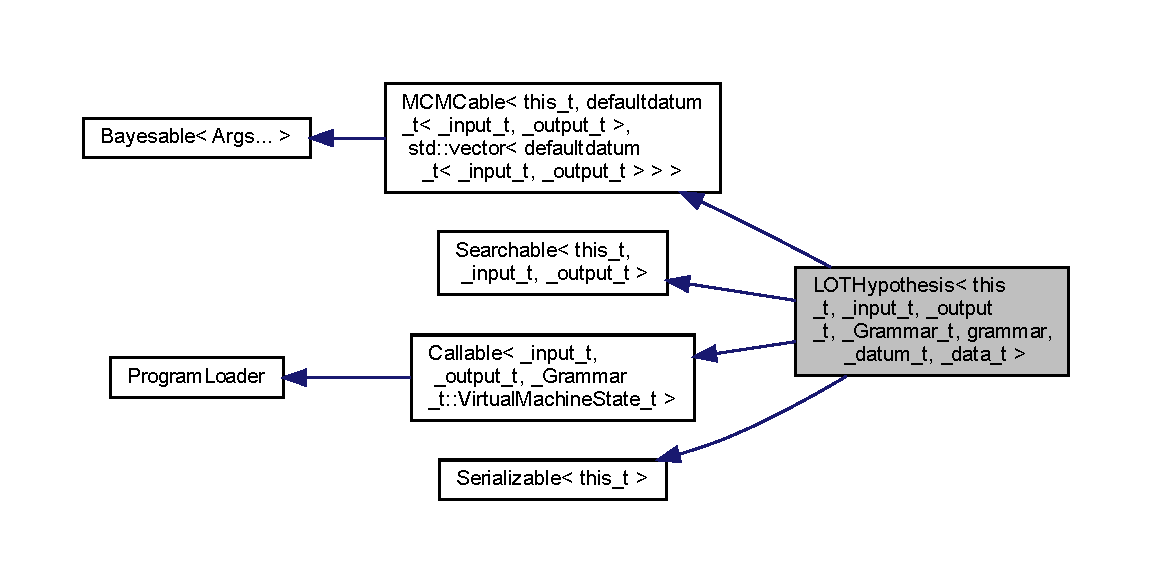
\includegraphics[width=350pt]{class_l_o_t_hypothesis__inherit__graph}
\end{center}
\end{figure}


Collaboration diagram for L\+O\+T\+Hypothesis$<$ this\+\_\+t, \+\_\+input\+\_\+t, \+\_\+output\+\_\+t, \+\_\+\+Grammar\+\_\+t, grammar, \+\_\+datum\+\_\+t, \+\_\+data\+\_\+t, \+\_\+\+Virtual\+Machine\+State\+\_\+t $>$\+:
\nopagebreak
\begin{figure}[H]
\begin{center}
\leavevmode
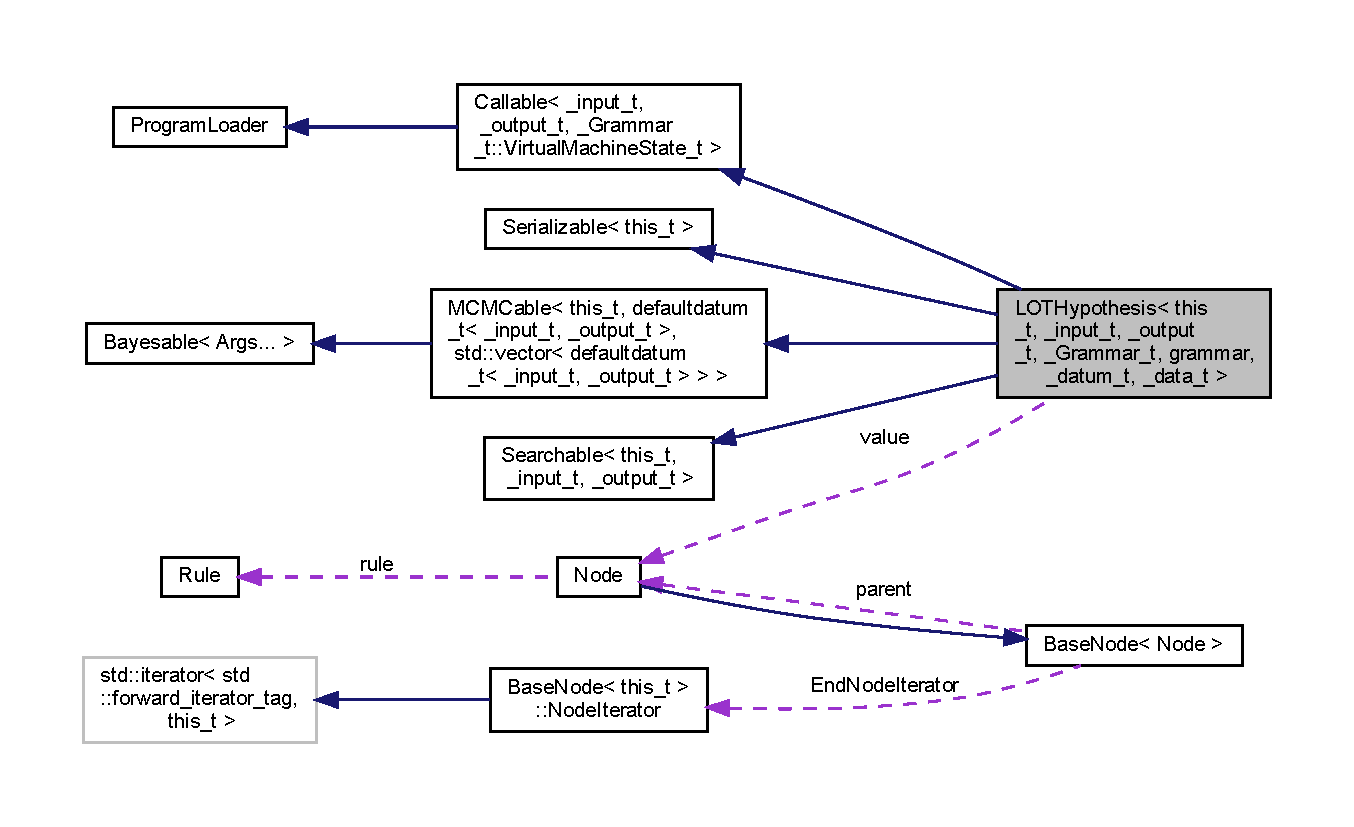
\includegraphics[width=350pt]{class_l_o_t_hypothesis__coll__graph}
\end{center}
\end{figure}
\doxysubsection*{Public Types}
\begin{DoxyCompactItemize}
\item 
typedef \mbox{\hyperlink{class_bayesable}{Bayesable}}$<$ \+\_\+datum\+\_\+t, \+\_\+data\+\_\+t $>$\+::\mbox{\hyperlink{class_l_o_t_hypothesis_a35bdca8c200553a791aba339ce3ce3a3}{datum\+\_\+t}} \mbox{\hyperlink{class_l_o_t_hypothesis_a35bdca8c200553a791aba339ce3ce3a3}{datum\+\_\+t}}
\item 
typedef \mbox{\hyperlink{class_bayesable}{Bayesable}}$<$ \+\_\+datum\+\_\+t, \+\_\+data\+\_\+t $>$\+::\mbox{\hyperlink{class_l_o_t_hypothesis_a003d6fac875d4223d3b4cd69a2bd6e0b}{data\+\_\+t}} \mbox{\hyperlink{class_l_o_t_hypothesis_a003d6fac875d4223d3b4cd69a2bd6e0b}{data\+\_\+t}}
\item 
using \mbox{\hyperlink{class_l_o_t_hypothesis_aea8a655b606b49e2afd101913499915f}{Grammar\+\_\+t}} = \+\_\+\+Grammar\+\_\+t
\item 
using \mbox{\hyperlink{class_l_o_t_hypothesis_aad56e3ff6bdae00d73defa434658a487}{input\+\_\+t}} = \+\_\+input\+\_\+t
\item 
using \mbox{\hyperlink{class_l_o_t_hypothesis_aeca47f6ec628c77e629fa41247198b6a}{output\+\_\+t}} = \+\_\+output\+\_\+t
\item 
using \mbox{\hyperlink{class_l_o_t_hypothesis_aee006574a5f8f7b2b948af0d566d2bad}{Virtual\+Machine\+State\+\_\+t}} = \+\_\+\+Virtual\+Machine\+State\+\_\+t
\item 
using \mbox{\hyperlink{class_l_o_t_hypothesis_a56b055927dc4d3267c71eba75bfe9e0b}{Proposal\+Type}} = std\+::optional$<$ std\+::pair$<$ this\+\_\+t, double $>$ $>$
\end{DoxyCompactItemize}
\doxysubsection*{Public Member Functions}
\begin{DoxyCompactItemize}
\item 
\mbox{\hyperlink{class_l_o_t_hypothesis_a89790f81aa379d7082fb50c2d64e5f13}{L\+O\+T\+Hypothesis}} ()
\item 
\mbox{\hyperlink{class_l_o_t_hypothesis_abf3b2d382182ff02be9f13aa5fb13a16}{L\+O\+T\+Hypothesis}} (\mbox{\hyperlink{class_node}{Node}} \&x)
\item 
\mbox{\hyperlink{class_l_o_t_hypothesis_a41eac42b6f3bb0705c8d40a53ec55143}{L\+O\+T\+Hypothesis}} (\mbox{\hyperlink{class_node}{Node}} \&\&x)
\item 
\mbox{\hyperlink{class_l_o_t_hypothesis_adc525d09bb7b64dca68085c4e2566ad0}{L\+O\+T\+Hypothesis}} (std\+::string s)
\item 
\mbox{\hyperlink{class_l_o_t_hypothesis_adcd5892963796922c26010781579b10f}{L\+O\+T\+Hypothesis}} (const \mbox{\hyperlink{class_l_o_t_hypothesis}{L\+O\+T\+Hypothesis}} \&c)
\item 
\mbox{\hyperlink{class_l_o_t_hypothesis_a7de7359b0a205d9acf79dccef867f80f}{L\+O\+T\+Hypothesis}} (const \mbox{\hyperlink{class_l_o_t_hypothesis}{L\+O\+T\+Hypothesis}} \&\&c)
\item 
\mbox{\hyperlink{class_l_o_t_hypothesis}{L\+O\+T\+Hypothesis}} \& \mbox{\hyperlink{class_l_o_t_hypothesis_aca230d54f058116fbb44051a3586f035}{operator=}} (const \mbox{\hyperlink{class_l_o_t_hypothesis}{L\+O\+T\+Hypothesis}} \&c)
\item 
\mbox{\hyperlink{class_l_o_t_hypothesis}{L\+O\+T\+Hypothesis}} \& \mbox{\hyperlink{class_l_o_t_hypothesis_a04f286c6b2157c3b23995c79b1791089}{operator=}} (const \mbox{\hyperlink{class_l_o_t_hypothesis}{L\+O\+T\+Hypothesis}} \&\&c)
\item 
virtual \mbox{\hyperlink{class_l_o_t_hypothesis_a56b055927dc4d3267c71eba75bfe9e0b}{Proposal\+Type}} \mbox{\hyperlink{class_l_o_t_hypothesis_afaf1e27b95bb2e19a25fa65ab538e4f2}{propose}} () const override
\begin{DoxyCompactList}\small\item\em Default proposal is rational-\/rules style regeneration. \end{DoxyCompactList}\item 
virtual this\+\_\+t \mbox{\hyperlink{class_l_o_t_hypothesis_aa302e4e72c76aaee7902d7a8f71b0398}{restart}} () const override
\begin{DoxyCompactList}\small\item\em This is used to restart chains, sampling from prior but O\+N\+LY for nodes that are can\+\_\+resample. \end{DoxyCompactList}\item 
\mbox{\hyperlink{class_node}{Node}} \& \mbox{\hyperlink{class_l_o_t_hypothesis_a3d26ba540cdd45ccf7da8dccd14536ee}{get\+\_\+value}} ()
\item 
const \mbox{\hyperlink{class_node}{Node}} \& \mbox{\hyperlink{class_l_o_t_hypothesis_afa44e4d2e7070178e7e6f12e1b672516}{get\+\_\+value}} () const
\item 
void \mbox{\hyperlink{class_l_o_t_hypothesis_af4c0128f8fd37bb8a02418e2f58c2bc0}{set\+\_\+value}} (\mbox{\hyperlink{class_node}{Node}} \&v)
\begin{DoxyCompactList}\small\item\em Set the value to v. (N\+O\+TE\+: This compiles into a program) \end{DoxyCompactList}\item 
void \mbox{\hyperlink{class_l_o_t_hypothesis_a45e5d33cbe2edbfde8d54f44028e6b63}{set\+\_\+value}} (\mbox{\hyperlink{class_node}{Node}} \&\&v)
\item 
\mbox{\hyperlink{class_l_o_t_hypothesis_aea8a655b606b49e2afd101913499915f}{Grammar\+\_\+t}} $\ast$ \mbox{\hyperlink{class_l_o_t_hypothesis_a7aba7e03532a8b315038bad11f47bbf9}{get\+\_\+grammar}} () const
\item 
virtual double \mbox{\hyperlink{class_l_o_t_hypothesis_aeeff5760a4d0c2bc586618d51f38ac80}{compute\+\_\+prior}} () override
\begin{DoxyCompactList}\small\item\em Compute the prior -- defaultly just the P\+C\+FG (grammar) prior. \end{DoxyCompactList}\item 
virtual double \mbox{\hyperlink{class_l_o_t_hypothesis_a020bfe8e12d80add92c665518650c4cb}{compute\+\_\+single\+\_\+likelihood}} (const \mbox{\hyperlink{class_l_o_t_hypothesis_a35bdca8c200553a791aba339ce3ce3a3}{datum\+\_\+t}} \&datum) override
\item 
void \mbox{\hyperlink{class_l_o_t_hypothesis_a22550030c8f89e613d44a3c9c30b2ea2}{compile}} ()
\item 
virtual void \mbox{\hyperlink{class_l_o_t_hypothesis_a00d33f253d0982d399f1295675e9725f}{push\+\_\+program}} (\mbox{\hyperlink{class_program}{Program}}$<$ \mbox{\hyperlink{class_l_o_t_hypothesis_aee006574a5f8f7b2b948af0d566d2bad}{Virtual\+Machine\+State\+\_\+t}} $>$ \&s) override
\begin{DoxyCompactList}\small\item\em This puts the code from my node onto s. Used internally in e.\+g. recursion. \end{DoxyCompactList}\item 
virtual std\+::string \mbox{\hyperlink{class_l_o_t_hypothesis_a601690bfe4d9e9bf568ecc40e8746856}{string}} (std\+::string prefix=\char`\"{}\char`\"{}) const override
\item 
virtual std\+::string \mbox{\hyperlink{class_l_o_t_hypothesis_a99e3630cb26b22e1cbee62bd155198ff}{string}} (std\+::string prefix, bool usedot) const
\item 
virtual size\+\_\+t \mbox{\hyperlink{class_l_o_t_hypothesis_aa7c283cb0d68218cb1f869171c45dfb9}{hash}} () const override
\item 
virtual bool \mbox{\hyperlink{class_l_o_t_hypothesis_aab4eec5c502d4a3c11c93a81975fcde0}{operator==}} (const this\+\_\+t \&h) const override
\begin{DoxyCompactList}\small\item\em Equality is checked on equality of values; note that greater-\/than is still on posteriors. \end{DoxyCompactList}\item 
virtual void \mbox{\hyperlink{class_l_o_t_hypothesis_afda1517e3cc79e871ecfbd7989f05530}{complete}} () override
\begin{DoxyCompactList}\small\item\em Modify this hypothesis\textquotesingle{}s value by filling in all the gaps. \end{DoxyCompactList}\item 
virtual int \mbox{\hyperlink{class_l_o_t_hypothesis_a5246924e3dbeff77e7c3f682fe7d3bd0}{neighbors}} () const override
\begin{DoxyCompactList}\small\item\em A variant of call that assumes no stochasticity and therefore outputs only a single value. (This uses a nullptr virtual machine pool, so will throw an error on flip) \end{DoxyCompactList}\item 
virtual void \mbox{\hyperlink{class_l_o_t_hypothesis_aef1f480e342420aa2a2c657c6650f47c}{expand\+\_\+to\+\_\+neighbor}} (int k) override
\begin{DoxyCompactList}\small\item\em Modify this hypothesis to become the k\textquotesingle{}th neighbor. N\+O\+TE This does not compile since it might not be complete. \end{DoxyCompactList}\item 
virtual double \mbox{\hyperlink{class_l_o_t_hypothesis_a2f1f9f66b9037f6a3560561c1a5fe72b}{neighbor\+\_\+prior}} (int k) override
\begin{DoxyCompactList}\small\item\em What is the prior of the k\textquotesingle{}th neighbor? This does not need to return the full prior, only relative (among ks) \end{DoxyCompactList}\item 
virtual bool \mbox{\hyperlink{class_l_o_t_hypothesis_a451b928d380be4834386fba14312b56a}{is\+\_\+evaluable}} () const override
\begin{DoxyCompactList}\small\item\em A node is \char`\"{}evaluable\char`\"{} if it is complete (meaning no null subnodes) \end{DoxyCompactList}\item 
size\+\_\+t \mbox{\hyperlink{class_l_o_t_hypothesis_a754c906d7c93fb59d142e1f506ac8234}{recursion\+\_\+count}} ()
\begin{DoxyCompactList}\small\item\em Count up how many times I use recursion -- we keep a list of recursion here. \end{DoxyCompactList}\item 
virtual std\+::string \mbox{\hyperlink{class_l_o_t_hypothesis_a5fc6e161f67c02a174955cd55a373a99}{serialize}} () const override
\begin{DoxyCompactList}\small\item\em Convert this into a string which can be written to a file. \end{DoxyCompactList}\end{DoxyCompactItemize}
\doxysubsection*{Static Public Member Functions}
\begin{DoxyCompactItemize}
\item 
static this\+\_\+t \mbox{\hyperlink{class_l_o_t_hypothesis_aba852f52c5979b542402be563882f421}{sample}} ()
\item 
static this\+\_\+t \mbox{\hyperlink{class_l_o_t_hypothesis_aa0301c2b0764b84b8a51c7b5bf5e521c}{from\+\_\+string}} (\mbox{\hyperlink{class_l_o_t_hypothesis_aea8a655b606b49e2afd101913499915f}{Grammar\+\_\+t}} $\ast$g, std\+::string s)
\item 
static this\+\_\+t \mbox{\hyperlink{class_l_o_t_hypothesis_ab8a5f36d43fb9726a7ef92e2d647781a}{deserialize}} (const std\+::string \&s)
\begin{DoxyCompactList}\small\item\em Convert this from a string which was in a file. \end{DoxyCompactList}\end{DoxyCompactItemize}
\doxysubsection*{Public Attributes}
\begin{DoxyCompactItemize}
\item 
unsigned long \mbox{\hyperlink{class_l_o_t_hypothesis_a8386c18cc6aaab810e81b990598ad4f8}{total\+\_\+instruction\+\_\+count\+\_\+last\+\_\+call}}
\item 
unsigned long \mbox{\hyperlink{class_l_o_t_hypothesis_a72acd311adb60509777dbb490cb04a3c}{total\+\_\+vms\+\_\+steps}}
\item 
\mbox{\hyperlink{class_program}{Program}}$<$ \mbox{\hyperlink{class_l_o_t_hypothesis_aee006574a5f8f7b2b948af0d566d2bad}{Virtual\+Machine\+State\+\_\+t}} $>$ \mbox{\hyperlink{class_l_o_t_hypothesis_a9f76b52b945e1f26e7af2c89584732e9}{program}}
\end{DoxyCompactItemize}
\doxysubsection*{Static Public Attributes}
\begin{DoxyCompactItemize}
\item 
static const char \mbox{\hyperlink{class_l_o_t_hypothesis_a060f79efcbf1a515fc0410cc03ab161d}{Serialization\+Delimiter}} = \textquotesingle{}\textbackslash{}t\textquotesingle{}
\item 
static const size\+\_\+t \mbox{\hyperlink{class_l_o_t_hypothesis_ab06d3217b08d3214654bce5fc7691ef4}{M\+A\+X\+\_\+\+N\+O\+D\+ES}} = 64
\end{DoxyCompactItemize}
\doxysubsection*{Protected Attributes}
\begin{DoxyCompactItemize}
\item 
\mbox{\hyperlink{class_node}{Node}} \mbox{\hyperlink{class_l_o_t_hypothesis_a7c7d4f528ebfb48dec31b2a780564143}{value}}
\end{DoxyCompactItemize}


\doxysubsection{Detailed Description}
\subsubsection*{template$<$typename this\+\_\+t, typename \+\_\+input\+\_\+t, typename \+\_\+output\+\_\+t, typename \+\_\+\+Grammar\+\_\+t, \+\_\+\+Grammar\+\_\+t $\ast$ grammar, typename \+\_\+datum\+\_\+t = defaultdatum\+\_\+t$<$\+\_\+input\+\_\+t, \+\_\+output\+\_\+t$>$, typename \+\_\+data\+\_\+t = std\+::vector$<$\+\_\+datum\+\_\+t$>$, typename \+\_\+\+Virtual\+Machine\+State\+\_\+t = typename \+\_\+\+Grammar\+\_\+t\+::\+Virtual\+Machine\+State\+\_\+t$>$\newline
class L\+O\+T\+Hypothesis$<$ this\+\_\+t, \+\_\+input\+\_\+t, \+\_\+output\+\_\+t, \+\_\+\+Grammar\+\_\+t, grammar, \+\_\+datum\+\_\+t, \+\_\+data\+\_\+t, \+\_\+\+Virtual\+Machine\+State\+\_\+t $>$}

\begin{DoxyAuthor}{Author}
piantado 
\end{DoxyAuthor}
\begin{DoxyDate}{Date}
05/05/20 
\end{DoxyDate}


\doxysubsection{Member Typedef Documentation}
\mbox{\Hypertarget{class_l_o_t_hypothesis_a003d6fac875d4223d3b4cd69a2bd6e0b}\label{class_l_o_t_hypothesis_a003d6fac875d4223d3b4cd69a2bd6e0b}} 
\index{LOTHypothesis$<$ this\_t, \_input\_t, \_output\_t, \_Grammar\_t, grammar, \_datum\_t, \_data\_t, \_VirtualMachineState\_t $>$@{LOTHypothesis$<$ this\_t, \_input\_t, \_output\_t, \_Grammar\_t, grammar, \_datum\_t, \_data\_t, \_VirtualMachineState\_t $>$}!data\_t@{data\_t}}
\index{data\_t@{data\_t}!LOTHypothesis$<$ this\_t, \_input\_t, \_output\_t, \_Grammar\_t, grammar, \_datum\_t, \_data\_t, \_VirtualMachineState\_t $>$@{LOTHypothesis$<$ this\_t, \_input\_t, \_output\_t, \_Grammar\_t, grammar, \_datum\_t, \_data\_t, \_VirtualMachineState\_t $>$}}
\doxysubsubsection{\texorpdfstring{data\_t}{data\_t}}
{\footnotesize\ttfamily template$<$typename this\+\_\+t , typename \+\_\+input\+\_\+t , typename \+\_\+output\+\_\+t , typename \+\_\+\+Grammar\+\_\+t , \+\_\+\+Grammar\+\_\+t $\ast$ grammar, typename \+\_\+datum\+\_\+t  = defaultdatum\+\_\+t$<$\+\_\+input\+\_\+t, \+\_\+output\+\_\+t$>$, typename \+\_\+data\+\_\+t  = std\+::vector$<$\+\_\+datum\+\_\+t$>$, typename \+\_\+\+Virtual\+Machine\+State\+\_\+t  = typename \+\_\+\+Grammar\+\_\+t\+::\+Virtual\+Machine\+State\+\_\+t$>$ \\
typedef \mbox{\hyperlink{class_bayesable}{Bayesable}}$<$\+\_\+datum\+\_\+t,\+\_\+data\+\_\+t$>$\+::\mbox{\hyperlink{class_l_o_t_hypothesis_a003d6fac875d4223d3b4cd69a2bd6e0b}{data\+\_\+t}} \mbox{\hyperlink{class_l_o_t_hypothesis}{L\+O\+T\+Hypothesis}}$<$ this\+\_\+t, \+\_\+input\+\_\+t, \+\_\+output\+\_\+t, \+\_\+\+Grammar\+\_\+t, grammar, \+\_\+datum\+\_\+t, \+\_\+data\+\_\+t, \+\_\+\+Virtual\+Machine\+State\+\_\+t $>$\+::\mbox{\hyperlink{class_l_o_t_hypothesis_a003d6fac875d4223d3b4cd69a2bd6e0b}{data\+\_\+t}}}

\mbox{\Hypertarget{class_l_o_t_hypothesis_a35bdca8c200553a791aba339ce3ce3a3}\label{class_l_o_t_hypothesis_a35bdca8c200553a791aba339ce3ce3a3}} 
\index{LOTHypothesis$<$ this\_t, \_input\_t, \_output\_t, \_Grammar\_t, grammar, \_datum\_t, \_data\_t, \_VirtualMachineState\_t $>$@{LOTHypothesis$<$ this\_t, \_input\_t, \_output\_t, \_Grammar\_t, grammar, \_datum\_t, \_data\_t, \_VirtualMachineState\_t $>$}!datum\_t@{datum\_t}}
\index{datum\_t@{datum\_t}!LOTHypothesis$<$ this\_t, \_input\_t, \_output\_t, \_Grammar\_t, grammar, \_datum\_t, \_data\_t, \_VirtualMachineState\_t $>$@{LOTHypothesis$<$ this\_t, \_input\_t, \_output\_t, \_Grammar\_t, grammar, \_datum\_t, \_data\_t, \_VirtualMachineState\_t $>$}}
\doxysubsubsection{\texorpdfstring{datum\_t}{datum\_t}}
{\footnotesize\ttfamily template$<$typename this\+\_\+t , typename \+\_\+input\+\_\+t , typename \+\_\+output\+\_\+t , typename \+\_\+\+Grammar\+\_\+t , \+\_\+\+Grammar\+\_\+t $\ast$ grammar, typename \+\_\+datum\+\_\+t  = defaultdatum\+\_\+t$<$\+\_\+input\+\_\+t, \+\_\+output\+\_\+t$>$, typename \+\_\+data\+\_\+t  = std\+::vector$<$\+\_\+datum\+\_\+t$>$, typename \+\_\+\+Virtual\+Machine\+State\+\_\+t  = typename \+\_\+\+Grammar\+\_\+t\+::\+Virtual\+Machine\+State\+\_\+t$>$ \\
typedef \mbox{\hyperlink{class_bayesable}{Bayesable}}$<$\+\_\+datum\+\_\+t,\+\_\+data\+\_\+t$>$\+::\mbox{\hyperlink{class_l_o_t_hypothesis_a35bdca8c200553a791aba339ce3ce3a3}{datum\+\_\+t}} \mbox{\hyperlink{class_l_o_t_hypothesis}{L\+O\+T\+Hypothesis}}$<$ this\+\_\+t, \+\_\+input\+\_\+t, \+\_\+output\+\_\+t, \+\_\+\+Grammar\+\_\+t, grammar, \+\_\+datum\+\_\+t, \+\_\+data\+\_\+t, \+\_\+\+Virtual\+Machine\+State\+\_\+t $>$\+::\mbox{\hyperlink{class_l_o_t_hypothesis_a35bdca8c200553a791aba339ce3ce3a3}{datum\+\_\+t}}}

\mbox{\Hypertarget{class_l_o_t_hypothesis_aea8a655b606b49e2afd101913499915f}\label{class_l_o_t_hypothesis_aea8a655b606b49e2afd101913499915f}} 
\index{LOTHypothesis$<$ this\_t, \_input\_t, \_output\_t, \_Grammar\_t, grammar, \_datum\_t, \_data\_t, \_VirtualMachineState\_t $>$@{LOTHypothesis$<$ this\_t, \_input\_t, \_output\_t, \_Grammar\_t, grammar, \_datum\_t, \_data\_t, \_VirtualMachineState\_t $>$}!Grammar\_t@{Grammar\_t}}
\index{Grammar\_t@{Grammar\_t}!LOTHypothesis$<$ this\_t, \_input\_t, \_output\_t, \_Grammar\_t, grammar, \_datum\_t, \_data\_t, \_VirtualMachineState\_t $>$@{LOTHypothesis$<$ this\_t, \_input\_t, \_output\_t, \_Grammar\_t, grammar, \_datum\_t, \_data\_t, \_VirtualMachineState\_t $>$}}
\doxysubsubsection{\texorpdfstring{Grammar\_t}{Grammar\_t}}
{\footnotesize\ttfamily template$<$typename this\+\_\+t , typename \+\_\+input\+\_\+t , typename \+\_\+output\+\_\+t , typename \+\_\+\+Grammar\+\_\+t , \+\_\+\+Grammar\+\_\+t $\ast$ grammar, typename \+\_\+datum\+\_\+t  = defaultdatum\+\_\+t$<$\+\_\+input\+\_\+t, \+\_\+output\+\_\+t$>$, typename \+\_\+data\+\_\+t  = std\+::vector$<$\+\_\+datum\+\_\+t$>$, typename \+\_\+\+Virtual\+Machine\+State\+\_\+t  = typename \+\_\+\+Grammar\+\_\+t\+::\+Virtual\+Machine\+State\+\_\+t$>$ \\
using \mbox{\hyperlink{class_l_o_t_hypothesis}{L\+O\+T\+Hypothesis}}$<$ this\+\_\+t, \+\_\+input\+\_\+t, \+\_\+output\+\_\+t, \+\_\+\+Grammar\+\_\+t, grammar, \+\_\+datum\+\_\+t, \+\_\+data\+\_\+t, \+\_\+\+Virtual\+Machine\+State\+\_\+t $>$\+::\mbox{\hyperlink{class_l_o_t_hypothesis_aea8a655b606b49e2afd101913499915f}{Grammar\+\_\+t}} =  \+\_\+\+Grammar\+\_\+t}

\mbox{\Hypertarget{class_l_o_t_hypothesis_aad56e3ff6bdae00d73defa434658a487}\label{class_l_o_t_hypothesis_aad56e3ff6bdae00d73defa434658a487}} 
\index{LOTHypothesis$<$ this\_t, \_input\_t, \_output\_t, \_Grammar\_t, grammar, \_datum\_t, \_data\_t, \_VirtualMachineState\_t $>$@{LOTHypothesis$<$ this\_t, \_input\_t, \_output\_t, \_Grammar\_t, grammar, \_datum\_t, \_data\_t, \_VirtualMachineState\_t $>$}!input\_t@{input\_t}}
\index{input\_t@{input\_t}!LOTHypothesis$<$ this\_t, \_input\_t, \_output\_t, \_Grammar\_t, grammar, \_datum\_t, \_data\_t, \_VirtualMachineState\_t $>$@{LOTHypothesis$<$ this\_t, \_input\_t, \_output\_t, \_Grammar\_t, grammar, \_datum\_t, \_data\_t, \_VirtualMachineState\_t $>$}}
\doxysubsubsection{\texorpdfstring{input\_t}{input\_t}}
{\footnotesize\ttfamily template$<$typename this\+\_\+t , typename \+\_\+input\+\_\+t , typename \+\_\+output\+\_\+t , typename \+\_\+\+Grammar\+\_\+t , \+\_\+\+Grammar\+\_\+t $\ast$ grammar, typename \+\_\+datum\+\_\+t  = defaultdatum\+\_\+t$<$\+\_\+input\+\_\+t, \+\_\+output\+\_\+t$>$, typename \+\_\+data\+\_\+t  = std\+::vector$<$\+\_\+datum\+\_\+t$>$, typename \+\_\+\+Virtual\+Machine\+State\+\_\+t  = typename \+\_\+\+Grammar\+\_\+t\+::\+Virtual\+Machine\+State\+\_\+t$>$ \\
using \mbox{\hyperlink{class_l_o_t_hypothesis}{L\+O\+T\+Hypothesis}}$<$ this\+\_\+t, \+\_\+input\+\_\+t, \+\_\+output\+\_\+t, \+\_\+\+Grammar\+\_\+t, grammar, \+\_\+datum\+\_\+t, \+\_\+data\+\_\+t, \+\_\+\+Virtual\+Machine\+State\+\_\+t $>$\+::\mbox{\hyperlink{class_l_o_t_hypothesis_aad56e3ff6bdae00d73defa434658a487}{input\+\_\+t}} =  \+\_\+input\+\_\+t}

\mbox{\Hypertarget{class_l_o_t_hypothesis_aeca47f6ec628c77e629fa41247198b6a}\label{class_l_o_t_hypothesis_aeca47f6ec628c77e629fa41247198b6a}} 
\index{LOTHypothesis$<$ this\_t, \_input\_t, \_output\_t, \_Grammar\_t, grammar, \_datum\_t, \_data\_t, \_VirtualMachineState\_t $>$@{LOTHypothesis$<$ this\_t, \_input\_t, \_output\_t, \_Grammar\_t, grammar, \_datum\_t, \_data\_t, \_VirtualMachineState\_t $>$}!output\_t@{output\_t}}
\index{output\_t@{output\_t}!LOTHypothesis$<$ this\_t, \_input\_t, \_output\_t, \_Grammar\_t, grammar, \_datum\_t, \_data\_t, \_VirtualMachineState\_t $>$@{LOTHypothesis$<$ this\_t, \_input\_t, \_output\_t, \_Grammar\_t, grammar, \_datum\_t, \_data\_t, \_VirtualMachineState\_t $>$}}
\doxysubsubsection{\texorpdfstring{output\_t}{output\_t}}
{\footnotesize\ttfamily template$<$typename this\+\_\+t , typename \+\_\+input\+\_\+t , typename \+\_\+output\+\_\+t , typename \+\_\+\+Grammar\+\_\+t , \+\_\+\+Grammar\+\_\+t $\ast$ grammar, typename \+\_\+datum\+\_\+t  = defaultdatum\+\_\+t$<$\+\_\+input\+\_\+t, \+\_\+output\+\_\+t$>$, typename \+\_\+data\+\_\+t  = std\+::vector$<$\+\_\+datum\+\_\+t$>$, typename \+\_\+\+Virtual\+Machine\+State\+\_\+t  = typename \+\_\+\+Grammar\+\_\+t\+::\+Virtual\+Machine\+State\+\_\+t$>$ \\
using \mbox{\hyperlink{class_l_o_t_hypothesis}{L\+O\+T\+Hypothesis}}$<$ this\+\_\+t, \+\_\+input\+\_\+t, \+\_\+output\+\_\+t, \+\_\+\+Grammar\+\_\+t, grammar, \+\_\+datum\+\_\+t, \+\_\+data\+\_\+t, \+\_\+\+Virtual\+Machine\+State\+\_\+t $>$\+::\mbox{\hyperlink{class_l_o_t_hypothesis_aeca47f6ec628c77e629fa41247198b6a}{output\+\_\+t}} =  \+\_\+output\+\_\+t}

\mbox{\Hypertarget{class_l_o_t_hypothesis_a56b055927dc4d3267c71eba75bfe9e0b}\label{class_l_o_t_hypothesis_a56b055927dc4d3267c71eba75bfe9e0b}} 
\index{LOTHypothesis$<$ this\_t, \_input\_t, \_output\_t, \_Grammar\_t, grammar, \_datum\_t, \_data\_t, \_VirtualMachineState\_t $>$@{LOTHypothesis$<$ this\_t, \_input\_t, \_output\_t, \_Grammar\_t, grammar, \_datum\_t, \_data\_t, \_VirtualMachineState\_t $>$}!ProposalType@{ProposalType}}
\index{ProposalType@{ProposalType}!LOTHypothesis$<$ this\_t, \_input\_t, \_output\_t, \_Grammar\_t, grammar, \_datum\_t, \_data\_t, \_VirtualMachineState\_t $>$@{LOTHypothesis$<$ this\_t, \_input\_t, \_output\_t, \_Grammar\_t, grammar, \_datum\_t, \_data\_t, \_VirtualMachineState\_t $>$}}
\doxysubsubsection{\texorpdfstring{ProposalType}{ProposalType}}
{\footnotesize\ttfamily template$<$typename this\+\_\+t , typename \+\_\+input\+\_\+t , typename \+\_\+output\+\_\+t , typename \+\_\+\+Grammar\+\_\+t , \+\_\+\+Grammar\+\_\+t $\ast$ grammar, typename \+\_\+datum\+\_\+t  = defaultdatum\+\_\+t$<$\+\_\+input\+\_\+t, \+\_\+output\+\_\+t$>$, typename \+\_\+data\+\_\+t  = std\+::vector$<$\+\_\+datum\+\_\+t$>$, typename \+\_\+\+Virtual\+Machine\+State\+\_\+t  = typename \+\_\+\+Grammar\+\_\+t\+::\+Virtual\+Machine\+State\+\_\+t$>$ \\
using \mbox{\hyperlink{class_l_o_t_hypothesis}{L\+O\+T\+Hypothesis}}$<$ this\+\_\+t, \+\_\+input\+\_\+t, \+\_\+output\+\_\+t, \+\_\+\+Grammar\+\_\+t, grammar, \+\_\+datum\+\_\+t, \+\_\+data\+\_\+t, \+\_\+\+Virtual\+Machine\+State\+\_\+t $>$\+::\mbox{\hyperlink{class_l_o_t_hypothesis_a56b055927dc4d3267c71eba75bfe9e0b}{Proposal\+Type}} =  std\+::optional$<$std\+::pair$<$this\+\_\+t,double$>$ $>$}

\mbox{\Hypertarget{class_l_o_t_hypothesis_aee006574a5f8f7b2b948af0d566d2bad}\label{class_l_o_t_hypothesis_aee006574a5f8f7b2b948af0d566d2bad}} 
\index{LOTHypothesis$<$ this\_t, \_input\_t, \_output\_t, \_Grammar\_t, grammar, \_datum\_t, \_data\_t, \_VirtualMachineState\_t $>$@{LOTHypothesis$<$ this\_t, \_input\_t, \_output\_t, \_Grammar\_t, grammar, \_datum\_t, \_data\_t, \_VirtualMachineState\_t $>$}!VirtualMachineState\_t@{VirtualMachineState\_t}}
\index{VirtualMachineState\_t@{VirtualMachineState\_t}!LOTHypothesis$<$ this\_t, \_input\_t, \_output\_t, \_Grammar\_t, grammar, \_datum\_t, \_data\_t, \_VirtualMachineState\_t $>$@{LOTHypothesis$<$ this\_t, \_input\_t, \_output\_t, \_Grammar\_t, grammar, \_datum\_t, \_data\_t, \_VirtualMachineState\_t $>$}}
\doxysubsubsection{\texorpdfstring{VirtualMachineState\_t}{VirtualMachineState\_t}}
{\footnotesize\ttfamily template$<$typename this\+\_\+t , typename \+\_\+input\+\_\+t , typename \+\_\+output\+\_\+t , typename \+\_\+\+Grammar\+\_\+t , \+\_\+\+Grammar\+\_\+t $\ast$ grammar, typename \+\_\+datum\+\_\+t  = defaultdatum\+\_\+t$<$\+\_\+input\+\_\+t, \+\_\+output\+\_\+t$>$, typename \+\_\+data\+\_\+t  = std\+::vector$<$\+\_\+datum\+\_\+t$>$, typename \+\_\+\+Virtual\+Machine\+State\+\_\+t  = typename \+\_\+\+Grammar\+\_\+t\+::\+Virtual\+Machine\+State\+\_\+t$>$ \\
using \mbox{\hyperlink{class_l_o_t_hypothesis}{L\+O\+T\+Hypothesis}}$<$ this\+\_\+t, \+\_\+input\+\_\+t, \+\_\+output\+\_\+t, \+\_\+\+Grammar\+\_\+t, grammar, \+\_\+datum\+\_\+t, \+\_\+data\+\_\+t, \+\_\+\+Virtual\+Machine\+State\+\_\+t $>$\+::\mbox{\hyperlink{class_l_o_t_hypothesis_aee006574a5f8f7b2b948af0d566d2bad}{Virtual\+Machine\+State\+\_\+t}} =  \+\_\+\+Virtual\+Machine\+State\+\_\+t}



\doxysubsection{Constructor \& Destructor Documentation}
\mbox{\Hypertarget{class_l_o_t_hypothesis_a89790f81aa379d7082fb50c2d64e5f13}\label{class_l_o_t_hypothesis_a89790f81aa379d7082fb50c2d64e5f13}} 
\index{LOTHypothesis$<$ this\_t, \_input\_t, \_output\_t, \_Grammar\_t, grammar, \_datum\_t, \_data\_t, \_VirtualMachineState\_t $>$@{LOTHypothesis$<$ this\_t, \_input\_t, \_output\_t, \_Grammar\_t, grammar, \_datum\_t, \_data\_t, \_VirtualMachineState\_t $>$}!LOTHypothesis@{LOTHypothesis}}
\index{LOTHypothesis@{LOTHypothesis}!LOTHypothesis$<$ this\_t, \_input\_t, \_output\_t, \_Grammar\_t, grammar, \_datum\_t, \_data\_t, \_VirtualMachineState\_t $>$@{LOTHypothesis$<$ this\_t, \_input\_t, \_output\_t, \_Grammar\_t, grammar, \_datum\_t, \_data\_t, \_VirtualMachineState\_t $>$}}
\doxysubsubsection{\texorpdfstring{LOTHypothesis()}{LOTHypothesis()}\hspace{0.1cm}{\footnotesize\ttfamily [1/6]}}
{\footnotesize\ttfamily template$<$typename this\+\_\+t , typename \+\_\+input\+\_\+t , typename \+\_\+output\+\_\+t , typename \+\_\+\+Grammar\+\_\+t , \+\_\+\+Grammar\+\_\+t $\ast$ grammar, typename \+\_\+datum\+\_\+t  = defaultdatum\+\_\+t$<$\+\_\+input\+\_\+t, \+\_\+output\+\_\+t$>$, typename \+\_\+data\+\_\+t  = std\+::vector$<$\+\_\+datum\+\_\+t$>$, typename \+\_\+\+Virtual\+Machine\+State\+\_\+t  = typename \+\_\+\+Grammar\+\_\+t\+::\+Virtual\+Machine\+State\+\_\+t$>$ \\
\mbox{\hyperlink{class_l_o_t_hypothesis}{L\+O\+T\+Hypothesis}}$<$ this\+\_\+t, \+\_\+input\+\_\+t, \+\_\+output\+\_\+t, \+\_\+\+Grammar\+\_\+t, grammar, \+\_\+datum\+\_\+t, \+\_\+data\+\_\+t, \+\_\+\+Virtual\+Machine\+State\+\_\+t $>$\+::\mbox{\hyperlink{class_l_o_t_hypothesis}{L\+O\+T\+Hypothesis}} (\begin{DoxyParamCaption}{ }\end{DoxyParamCaption})\hspace{0.3cm}{\ttfamily [inline]}}

\mbox{\Hypertarget{class_l_o_t_hypothesis_abf3b2d382182ff02be9f13aa5fb13a16}\label{class_l_o_t_hypothesis_abf3b2d382182ff02be9f13aa5fb13a16}} 
\index{LOTHypothesis$<$ this\_t, \_input\_t, \_output\_t, \_Grammar\_t, grammar, \_datum\_t, \_data\_t, \_VirtualMachineState\_t $>$@{LOTHypothesis$<$ this\_t, \_input\_t, \_output\_t, \_Grammar\_t, grammar, \_datum\_t, \_data\_t, \_VirtualMachineState\_t $>$}!LOTHypothesis@{LOTHypothesis}}
\index{LOTHypothesis@{LOTHypothesis}!LOTHypothesis$<$ this\_t, \_input\_t, \_output\_t, \_Grammar\_t, grammar, \_datum\_t, \_data\_t, \_VirtualMachineState\_t $>$@{LOTHypothesis$<$ this\_t, \_input\_t, \_output\_t, \_Grammar\_t, grammar, \_datum\_t, \_data\_t, \_VirtualMachineState\_t $>$}}
\doxysubsubsection{\texorpdfstring{LOTHypothesis()}{LOTHypothesis()}\hspace{0.1cm}{\footnotesize\ttfamily [2/6]}}
{\footnotesize\ttfamily template$<$typename this\+\_\+t , typename \+\_\+input\+\_\+t , typename \+\_\+output\+\_\+t , typename \+\_\+\+Grammar\+\_\+t , \+\_\+\+Grammar\+\_\+t $\ast$ grammar, typename \+\_\+datum\+\_\+t  = defaultdatum\+\_\+t$<$\+\_\+input\+\_\+t, \+\_\+output\+\_\+t$>$, typename \+\_\+data\+\_\+t  = std\+::vector$<$\+\_\+datum\+\_\+t$>$, typename \+\_\+\+Virtual\+Machine\+State\+\_\+t  = typename \+\_\+\+Grammar\+\_\+t\+::\+Virtual\+Machine\+State\+\_\+t$>$ \\
\mbox{\hyperlink{class_l_o_t_hypothesis}{L\+O\+T\+Hypothesis}}$<$ this\+\_\+t, \+\_\+input\+\_\+t, \+\_\+output\+\_\+t, \+\_\+\+Grammar\+\_\+t, grammar, \+\_\+datum\+\_\+t, \+\_\+data\+\_\+t, \+\_\+\+Virtual\+Machine\+State\+\_\+t $>$\+::\mbox{\hyperlink{class_l_o_t_hypothesis}{L\+O\+T\+Hypothesis}} (\begin{DoxyParamCaption}\item[{\mbox{\hyperlink{class_node}{Node}} \&}]{x }\end{DoxyParamCaption})\hspace{0.3cm}{\ttfamily [inline]}}

\mbox{\Hypertarget{class_l_o_t_hypothesis_a41eac42b6f3bb0705c8d40a53ec55143}\label{class_l_o_t_hypothesis_a41eac42b6f3bb0705c8d40a53ec55143}} 
\index{LOTHypothesis$<$ this\_t, \_input\_t, \_output\_t, \_Grammar\_t, grammar, \_datum\_t, \_data\_t, \_VirtualMachineState\_t $>$@{LOTHypothesis$<$ this\_t, \_input\_t, \_output\_t, \_Grammar\_t, grammar, \_datum\_t, \_data\_t, \_VirtualMachineState\_t $>$}!LOTHypothesis@{LOTHypothesis}}
\index{LOTHypothesis@{LOTHypothesis}!LOTHypothesis$<$ this\_t, \_input\_t, \_output\_t, \_Grammar\_t, grammar, \_datum\_t, \_data\_t, \_VirtualMachineState\_t $>$@{LOTHypothesis$<$ this\_t, \_input\_t, \_output\_t, \_Grammar\_t, grammar, \_datum\_t, \_data\_t, \_VirtualMachineState\_t $>$}}
\doxysubsubsection{\texorpdfstring{LOTHypothesis()}{LOTHypothesis()}\hspace{0.1cm}{\footnotesize\ttfamily [3/6]}}
{\footnotesize\ttfamily template$<$typename this\+\_\+t , typename \+\_\+input\+\_\+t , typename \+\_\+output\+\_\+t , typename \+\_\+\+Grammar\+\_\+t , \+\_\+\+Grammar\+\_\+t $\ast$ grammar, typename \+\_\+datum\+\_\+t  = defaultdatum\+\_\+t$<$\+\_\+input\+\_\+t, \+\_\+output\+\_\+t$>$, typename \+\_\+data\+\_\+t  = std\+::vector$<$\+\_\+datum\+\_\+t$>$, typename \+\_\+\+Virtual\+Machine\+State\+\_\+t  = typename \+\_\+\+Grammar\+\_\+t\+::\+Virtual\+Machine\+State\+\_\+t$>$ \\
\mbox{\hyperlink{class_l_o_t_hypothesis}{L\+O\+T\+Hypothesis}}$<$ this\+\_\+t, \+\_\+input\+\_\+t, \+\_\+output\+\_\+t, \+\_\+\+Grammar\+\_\+t, grammar, \+\_\+datum\+\_\+t, \+\_\+data\+\_\+t, \+\_\+\+Virtual\+Machine\+State\+\_\+t $>$\+::\mbox{\hyperlink{class_l_o_t_hypothesis}{L\+O\+T\+Hypothesis}} (\begin{DoxyParamCaption}\item[{\mbox{\hyperlink{class_node}{Node}} \&\&}]{x }\end{DoxyParamCaption})\hspace{0.3cm}{\ttfamily [inline]}}

\mbox{\Hypertarget{class_l_o_t_hypothesis_adc525d09bb7b64dca68085c4e2566ad0}\label{class_l_o_t_hypothesis_adc525d09bb7b64dca68085c4e2566ad0}} 
\index{LOTHypothesis$<$ this\_t, \_input\_t, \_output\_t, \_Grammar\_t, grammar, \_datum\_t, \_data\_t, \_VirtualMachineState\_t $>$@{LOTHypothesis$<$ this\_t, \_input\_t, \_output\_t, \_Grammar\_t, grammar, \_datum\_t, \_data\_t, \_VirtualMachineState\_t $>$}!LOTHypothesis@{LOTHypothesis}}
\index{LOTHypothesis@{LOTHypothesis}!LOTHypothesis$<$ this\_t, \_input\_t, \_output\_t, \_Grammar\_t, grammar, \_datum\_t, \_data\_t, \_VirtualMachineState\_t $>$@{LOTHypothesis$<$ this\_t, \_input\_t, \_output\_t, \_Grammar\_t, grammar, \_datum\_t, \_data\_t, \_VirtualMachineState\_t $>$}}
\doxysubsubsection{\texorpdfstring{LOTHypothesis()}{LOTHypothesis()}\hspace{0.1cm}{\footnotesize\ttfamily [4/6]}}
{\footnotesize\ttfamily template$<$typename this\+\_\+t , typename \+\_\+input\+\_\+t , typename \+\_\+output\+\_\+t , typename \+\_\+\+Grammar\+\_\+t , \+\_\+\+Grammar\+\_\+t $\ast$ grammar, typename \+\_\+datum\+\_\+t  = defaultdatum\+\_\+t$<$\+\_\+input\+\_\+t, \+\_\+output\+\_\+t$>$, typename \+\_\+data\+\_\+t  = std\+::vector$<$\+\_\+datum\+\_\+t$>$, typename \+\_\+\+Virtual\+Machine\+State\+\_\+t  = typename \+\_\+\+Grammar\+\_\+t\+::\+Virtual\+Machine\+State\+\_\+t$>$ \\
\mbox{\hyperlink{class_l_o_t_hypothesis}{L\+O\+T\+Hypothesis}}$<$ this\+\_\+t, \+\_\+input\+\_\+t, \+\_\+output\+\_\+t, \+\_\+\+Grammar\+\_\+t, grammar, \+\_\+datum\+\_\+t, \+\_\+data\+\_\+t, \+\_\+\+Virtual\+Machine\+State\+\_\+t $>$\+::\mbox{\hyperlink{class_l_o_t_hypothesis}{L\+O\+T\+Hypothesis}} (\begin{DoxyParamCaption}\item[{std\+::string}]{s }\end{DoxyParamCaption})\hspace{0.3cm}{\ttfamily [inline]}}

\mbox{\Hypertarget{class_l_o_t_hypothesis_adcd5892963796922c26010781579b10f}\label{class_l_o_t_hypothesis_adcd5892963796922c26010781579b10f}} 
\index{LOTHypothesis$<$ this\_t, \_input\_t, \_output\_t, \_Grammar\_t, grammar, \_datum\_t, \_data\_t, \_VirtualMachineState\_t $>$@{LOTHypothesis$<$ this\_t, \_input\_t, \_output\_t, \_Grammar\_t, grammar, \_datum\_t, \_data\_t, \_VirtualMachineState\_t $>$}!LOTHypothesis@{LOTHypothesis}}
\index{LOTHypothesis@{LOTHypothesis}!LOTHypothesis$<$ this\_t, \_input\_t, \_output\_t, \_Grammar\_t, grammar, \_datum\_t, \_data\_t, \_VirtualMachineState\_t $>$@{LOTHypothesis$<$ this\_t, \_input\_t, \_output\_t, \_Grammar\_t, grammar, \_datum\_t, \_data\_t, \_VirtualMachineState\_t $>$}}
\doxysubsubsection{\texorpdfstring{LOTHypothesis()}{LOTHypothesis()}\hspace{0.1cm}{\footnotesize\ttfamily [5/6]}}
{\footnotesize\ttfamily template$<$typename this\+\_\+t , typename \+\_\+input\+\_\+t , typename \+\_\+output\+\_\+t , typename \+\_\+\+Grammar\+\_\+t , \+\_\+\+Grammar\+\_\+t $\ast$ grammar, typename \+\_\+datum\+\_\+t  = defaultdatum\+\_\+t$<$\+\_\+input\+\_\+t, \+\_\+output\+\_\+t$>$, typename \+\_\+data\+\_\+t  = std\+::vector$<$\+\_\+datum\+\_\+t$>$, typename \+\_\+\+Virtual\+Machine\+State\+\_\+t  = typename \+\_\+\+Grammar\+\_\+t\+::\+Virtual\+Machine\+State\+\_\+t$>$ \\
\mbox{\hyperlink{class_l_o_t_hypothesis}{L\+O\+T\+Hypothesis}}$<$ this\+\_\+t, \+\_\+input\+\_\+t, \+\_\+output\+\_\+t, \+\_\+\+Grammar\+\_\+t, grammar, \+\_\+datum\+\_\+t, \+\_\+data\+\_\+t, \+\_\+\+Virtual\+Machine\+State\+\_\+t $>$\+::\mbox{\hyperlink{class_l_o_t_hypothesis}{L\+O\+T\+Hypothesis}} (\begin{DoxyParamCaption}\item[{const \mbox{\hyperlink{class_l_o_t_hypothesis}{L\+O\+T\+Hypothesis}}$<$ this\+\_\+t, \+\_\+input\+\_\+t, \+\_\+output\+\_\+t, \+\_\+\+Grammar\+\_\+t, grammar, \+\_\+datum\+\_\+t, \+\_\+data\+\_\+t, \+\_\+\+Virtual\+Machine\+State\+\_\+t $>$ \&}]{c }\end{DoxyParamCaption})\hspace{0.3cm}{\ttfamily [inline]}}

\mbox{\Hypertarget{class_l_o_t_hypothesis_a7de7359b0a205d9acf79dccef867f80f}\label{class_l_o_t_hypothesis_a7de7359b0a205d9acf79dccef867f80f}} 
\index{LOTHypothesis$<$ this\_t, \_input\_t, \_output\_t, \_Grammar\_t, grammar, \_datum\_t, \_data\_t, \_VirtualMachineState\_t $>$@{LOTHypothesis$<$ this\_t, \_input\_t, \_output\_t, \_Grammar\_t, grammar, \_datum\_t, \_data\_t, \_VirtualMachineState\_t $>$}!LOTHypothesis@{LOTHypothesis}}
\index{LOTHypothesis@{LOTHypothesis}!LOTHypothesis$<$ this\_t, \_input\_t, \_output\_t, \_Grammar\_t, grammar, \_datum\_t, \_data\_t, \_VirtualMachineState\_t $>$@{LOTHypothesis$<$ this\_t, \_input\_t, \_output\_t, \_Grammar\_t, grammar, \_datum\_t, \_data\_t, \_VirtualMachineState\_t $>$}}
\doxysubsubsection{\texorpdfstring{LOTHypothesis()}{LOTHypothesis()}\hspace{0.1cm}{\footnotesize\ttfamily [6/6]}}
{\footnotesize\ttfamily template$<$typename this\+\_\+t , typename \+\_\+input\+\_\+t , typename \+\_\+output\+\_\+t , typename \+\_\+\+Grammar\+\_\+t , \+\_\+\+Grammar\+\_\+t $\ast$ grammar, typename \+\_\+datum\+\_\+t  = defaultdatum\+\_\+t$<$\+\_\+input\+\_\+t, \+\_\+output\+\_\+t$>$, typename \+\_\+data\+\_\+t  = std\+::vector$<$\+\_\+datum\+\_\+t$>$, typename \+\_\+\+Virtual\+Machine\+State\+\_\+t  = typename \+\_\+\+Grammar\+\_\+t\+::\+Virtual\+Machine\+State\+\_\+t$>$ \\
\mbox{\hyperlink{class_l_o_t_hypothesis}{L\+O\+T\+Hypothesis}}$<$ this\+\_\+t, \+\_\+input\+\_\+t, \+\_\+output\+\_\+t, \+\_\+\+Grammar\+\_\+t, grammar, \+\_\+datum\+\_\+t, \+\_\+data\+\_\+t, \+\_\+\+Virtual\+Machine\+State\+\_\+t $>$\+::\mbox{\hyperlink{class_l_o_t_hypothesis}{L\+O\+T\+Hypothesis}} (\begin{DoxyParamCaption}\item[{const \mbox{\hyperlink{class_l_o_t_hypothesis}{L\+O\+T\+Hypothesis}}$<$ this\+\_\+t, \+\_\+input\+\_\+t, \+\_\+output\+\_\+t, \+\_\+\+Grammar\+\_\+t, grammar, \+\_\+datum\+\_\+t, \+\_\+data\+\_\+t, \+\_\+\+Virtual\+Machine\+State\+\_\+t $>$ \&\&}]{c }\end{DoxyParamCaption})\hspace{0.3cm}{\ttfamily [inline]}}



\doxysubsection{Member Function Documentation}
\mbox{\Hypertarget{class_l_o_t_hypothesis_a22550030c8f89e613d44a3c9c30b2ea2}\label{class_l_o_t_hypothesis_a22550030c8f89e613d44a3c9c30b2ea2}} 
\index{LOTHypothesis$<$ this\_t, \_input\_t, \_output\_t, \_Grammar\_t, grammar, \_datum\_t, \_data\_t, \_VirtualMachineState\_t $>$@{LOTHypothesis$<$ this\_t, \_input\_t, \_output\_t, \_Grammar\_t, grammar, \_datum\_t, \_data\_t, \_VirtualMachineState\_t $>$}!compile@{compile}}
\index{compile@{compile}!LOTHypothesis$<$ this\_t, \_input\_t, \_output\_t, \_Grammar\_t, grammar, \_datum\_t, \_data\_t, \_VirtualMachineState\_t $>$@{LOTHypothesis$<$ this\_t, \_input\_t, \_output\_t, \_Grammar\_t, grammar, \_datum\_t, \_data\_t, \_VirtualMachineState\_t $>$}}
\doxysubsubsection{\texorpdfstring{compile()}{compile()}}
{\footnotesize\ttfamily template$<$typename this\+\_\+t , typename \+\_\+input\+\_\+t , typename \+\_\+output\+\_\+t , typename \+\_\+\+Grammar\+\_\+t , \+\_\+\+Grammar\+\_\+t $\ast$ grammar, typename \+\_\+datum\+\_\+t  = defaultdatum\+\_\+t$<$\+\_\+input\+\_\+t, \+\_\+output\+\_\+t$>$, typename \+\_\+data\+\_\+t  = std\+::vector$<$\+\_\+datum\+\_\+t$>$, typename \+\_\+\+Virtual\+Machine\+State\+\_\+t  = typename \+\_\+\+Grammar\+\_\+t\+::\+Virtual\+Machine\+State\+\_\+t$>$ \\
void \mbox{\hyperlink{class_l_o_t_hypothesis}{L\+O\+T\+Hypothesis}}$<$ this\+\_\+t, \+\_\+input\+\_\+t, \+\_\+output\+\_\+t, \+\_\+\+Grammar\+\_\+t, grammar, \+\_\+datum\+\_\+t, \+\_\+data\+\_\+t, \+\_\+\+Virtual\+Machine\+State\+\_\+t $>$\+::compile (\begin{DoxyParamCaption}{ }\end{DoxyParamCaption})\hspace{0.3cm}{\ttfamily [inline]}}

\mbox{\Hypertarget{class_l_o_t_hypothesis_afda1517e3cc79e871ecfbd7989f05530}\label{class_l_o_t_hypothesis_afda1517e3cc79e871ecfbd7989f05530}} 
\index{LOTHypothesis$<$ this\_t, \_input\_t, \_output\_t, \_Grammar\_t, grammar, \_datum\_t, \_data\_t, \_VirtualMachineState\_t $>$@{LOTHypothesis$<$ this\_t, \_input\_t, \_output\_t, \_Grammar\_t, grammar, \_datum\_t, \_data\_t, \_VirtualMachineState\_t $>$}!complete@{complete}}
\index{complete@{complete}!LOTHypothesis$<$ this\_t, \_input\_t, \_output\_t, \_Grammar\_t, grammar, \_datum\_t, \_data\_t, \_VirtualMachineState\_t $>$@{LOTHypothesis$<$ this\_t, \_input\_t, \_output\_t, \_Grammar\_t, grammar, \_datum\_t, \_data\_t, \_VirtualMachineState\_t $>$}}
\doxysubsubsection{\texorpdfstring{complete()}{complete()}}
{\footnotesize\ttfamily template$<$typename this\+\_\+t , typename \+\_\+input\+\_\+t , typename \+\_\+output\+\_\+t , typename \+\_\+\+Grammar\+\_\+t , \+\_\+\+Grammar\+\_\+t $\ast$ grammar, typename \+\_\+datum\+\_\+t  = defaultdatum\+\_\+t$<$\+\_\+input\+\_\+t, \+\_\+output\+\_\+t$>$, typename \+\_\+data\+\_\+t  = std\+::vector$<$\+\_\+datum\+\_\+t$>$, typename \+\_\+\+Virtual\+Machine\+State\+\_\+t  = typename \+\_\+\+Grammar\+\_\+t\+::\+Virtual\+Machine\+State\+\_\+t$>$ \\
virtual void \mbox{\hyperlink{class_l_o_t_hypothesis}{L\+O\+T\+Hypothesis}}$<$ this\+\_\+t, \+\_\+input\+\_\+t, \+\_\+output\+\_\+t, \+\_\+\+Grammar\+\_\+t, grammar, \+\_\+datum\+\_\+t, \+\_\+data\+\_\+t, \+\_\+\+Virtual\+Machine\+State\+\_\+t $>$\+::complete (\begin{DoxyParamCaption}{ }\end{DoxyParamCaption})\hspace{0.3cm}{\ttfamily [inline]}, {\ttfamily [override]}, {\ttfamily [virtual]}}



Modify this hypothesis\textquotesingle{}s value by filling in all the gaps. 



Implements \mbox{\hyperlink{class_searchable_a29ab2eb0471e2e9d96d39f0349f21571}{Searchable$<$ this\+\_\+t, \+\_\+input\+\_\+t, \+\_\+output\+\_\+t $>$}}.

\mbox{\Hypertarget{class_l_o_t_hypothesis_aeeff5760a4d0c2bc586618d51f38ac80}\label{class_l_o_t_hypothesis_aeeff5760a4d0c2bc586618d51f38ac80}} 
\index{LOTHypothesis$<$ this\_t, \_input\_t, \_output\_t, \_Grammar\_t, grammar, \_datum\_t, \_data\_t, \_VirtualMachineState\_t $>$@{LOTHypothesis$<$ this\_t, \_input\_t, \_output\_t, \_Grammar\_t, grammar, \_datum\_t, \_data\_t, \_VirtualMachineState\_t $>$}!compute\_prior@{compute\_prior}}
\index{compute\_prior@{compute\_prior}!LOTHypothesis$<$ this\_t, \_input\_t, \_output\_t, \_Grammar\_t, grammar, \_datum\_t, \_data\_t, \_VirtualMachineState\_t $>$@{LOTHypothesis$<$ this\_t, \_input\_t, \_output\_t, \_Grammar\_t, grammar, \_datum\_t, \_data\_t, \_VirtualMachineState\_t $>$}}
\doxysubsubsection{\texorpdfstring{compute\_prior()}{compute\_prior()}}
{\footnotesize\ttfamily template$<$typename this\+\_\+t , typename \+\_\+input\+\_\+t , typename \+\_\+output\+\_\+t , typename \+\_\+\+Grammar\+\_\+t , \+\_\+\+Grammar\+\_\+t $\ast$ grammar, typename \+\_\+datum\+\_\+t  = defaultdatum\+\_\+t$<$\+\_\+input\+\_\+t, \+\_\+output\+\_\+t$>$, typename \+\_\+data\+\_\+t  = std\+::vector$<$\+\_\+datum\+\_\+t$>$, typename \+\_\+\+Virtual\+Machine\+State\+\_\+t  = typename \+\_\+\+Grammar\+\_\+t\+::\+Virtual\+Machine\+State\+\_\+t$>$ \\
virtual double \mbox{\hyperlink{class_l_o_t_hypothesis}{L\+O\+T\+Hypothesis}}$<$ this\+\_\+t, \+\_\+input\+\_\+t, \+\_\+output\+\_\+t, \+\_\+\+Grammar\+\_\+t, grammar, \+\_\+datum\+\_\+t, \+\_\+data\+\_\+t, \+\_\+\+Virtual\+Machine\+State\+\_\+t $>$\+::compute\+\_\+prior (\begin{DoxyParamCaption}{ }\end{DoxyParamCaption})\hspace{0.3cm}{\ttfamily [inline]}, {\ttfamily [override]}, {\ttfamily [virtual]}}



Compute the prior -- defaultly just the P\+C\+FG (grammar) prior. 

\begin{DoxyReturn}{Returns}

\end{DoxyReturn}


Implements \mbox{\hyperlink{class_bayesable_a1b057a17212ced123545133e2297c01b}{Bayesable$<$ Args... $>$}}.

\mbox{\Hypertarget{class_l_o_t_hypothesis_a020bfe8e12d80add92c665518650c4cb}\label{class_l_o_t_hypothesis_a020bfe8e12d80add92c665518650c4cb}} 
\index{LOTHypothesis$<$ this\_t, \_input\_t, \_output\_t, \_Grammar\_t, grammar, \_datum\_t, \_data\_t, \_VirtualMachineState\_t $>$@{LOTHypothesis$<$ this\_t, \_input\_t, \_output\_t, \_Grammar\_t, grammar, \_datum\_t, \_data\_t, \_VirtualMachineState\_t $>$}!compute\_single\_likelihood@{compute\_single\_likelihood}}
\index{compute\_single\_likelihood@{compute\_single\_likelihood}!LOTHypothesis$<$ this\_t, \_input\_t, \_output\_t, \_Grammar\_t, grammar, \_datum\_t, \_data\_t, \_VirtualMachineState\_t $>$@{LOTHypothesis$<$ this\_t, \_input\_t, \_output\_t, \_Grammar\_t, grammar, \_datum\_t, \_data\_t, \_VirtualMachineState\_t $>$}}
\doxysubsubsection{\texorpdfstring{compute\_single\_likelihood()}{compute\_single\_likelihood()}}
{\footnotesize\ttfamily template$<$typename this\+\_\+t , typename \+\_\+input\+\_\+t , typename \+\_\+output\+\_\+t , typename \+\_\+\+Grammar\+\_\+t , \+\_\+\+Grammar\+\_\+t $\ast$ grammar, typename \+\_\+datum\+\_\+t  = defaultdatum\+\_\+t$<$\+\_\+input\+\_\+t, \+\_\+output\+\_\+t$>$, typename \+\_\+data\+\_\+t  = std\+::vector$<$\+\_\+datum\+\_\+t$>$, typename \+\_\+\+Virtual\+Machine\+State\+\_\+t  = typename \+\_\+\+Grammar\+\_\+t\+::\+Virtual\+Machine\+State\+\_\+t$>$ \\
virtual double \mbox{\hyperlink{class_l_o_t_hypothesis}{L\+O\+T\+Hypothesis}}$<$ this\+\_\+t, \+\_\+input\+\_\+t, \+\_\+output\+\_\+t, \+\_\+\+Grammar\+\_\+t, grammar, \+\_\+datum\+\_\+t, \+\_\+data\+\_\+t, \+\_\+\+Virtual\+Machine\+State\+\_\+t $>$\+::compute\+\_\+single\+\_\+likelihood (\begin{DoxyParamCaption}\item[{const \mbox{\hyperlink{class_l_o_t_hypothesis_a35bdca8c200553a791aba339ce3ce3a3}{datum\+\_\+t}} \&}]{datum }\end{DoxyParamCaption})\hspace{0.3cm}{\ttfamily [inline]}, {\ttfamily [override]}, {\ttfamily [virtual]}}

\mbox{\Hypertarget{class_l_o_t_hypothesis_ab8a5f36d43fb9726a7ef92e2d647781a}\label{class_l_o_t_hypothesis_ab8a5f36d43fb9726a7ef92e2d647781a}} 
\index{LOTHypothesis$<$ this\_t, \_input\_t, \_output\_t, \_Grammar\_t, grammar, \_datum\_t, \_data\_t, \_VirtualMachineState\_t $>$@{LOTHypothesis$<$ this\_t, \_input\_t, \_output\_t, \_Grammar\_t, grammar, \_datum\_t, \_data\_t, \_VirtualMachineState\_t $>$}!deserialize@{deserialize}}
\index{deserialize@{deserialize}!LOTHypothesis$<$ this\_t, \_input\_t, \_output\_t, \_Grammar\_t, grammar, \_datum\_t, \_data\_t, \_VirtualMachineState\_t $>$@{LOTHypothesis$<$ this\_t, \_input\_t, \_output\_t, \_Grammar\_t, grammar, \_datum\_t, \_data\_t, \_VirtualMachineState\_t $>$}}
\doxysubsubsection{\texorpdfstring{deserialize()}{deserialize()}}
{\footnotesize\ttfamily template$<$typename this\+\_\+t , typename \+\_\+input\+\_\+t , typename \+\_\+output\+\_\+t , typename \+\_\+\+Grammar\+\_\+t , \+\_\+\+Grammar\+\_\+t $\ast$ grammar, typename \+\_\+datum\+\_\+t  = defaultdatum\+\_\+t$<$\+\_\+input\+\_\+t, \+\_\+output\+\_\+t$>$, typename \+\_\+data\+\_\+t  = std\+::vector$<$\+\_\+datum\+\_\+t$>$, typename \+\_\+\+Virtual\+Machine\+State\+\_\+t  = typename \+\_\+\+Grammar\+\_\+t\+::\+Virtual\+Machine\+State\+\_\+t$>$ \\
static this\+\_\+t \mbox{\hyperlink{class_l_o_t_hypothesis}{L\+O\+T\+Hypothesis}}$<$ this\+\_\+t, \+\_\+input\+\_\+t, \+\_\+output\+\_\+t, \+\_\+\+Grammar\+\_\+t, grammar, \+\_\+datum\+\_\+t, \+\_\+data\+\_\+t, \+\_\+\+Virtual\+Machine\+State\+\_\+t $>$\+::deserialize (\begin{DoxyParamCaption}\item[{const std\+::string \&}]{s }\end{DoxyParamCaption})\hspace{0.3cm}{\ttfamily [inline]}, {\ttfamily [static]}}



Convert this from a string which was in a file. 


\begin{DoxyParams}{Parameters}
{\em s} & \\
\hline
\end{DoxyParams}
\begin{DoxyReturn}{Returns}

\end{DoxyReturn}
\mbox{\Hypertarget{class_l_o_t_hypothesis_aef1f480e342420aa2a2c657c6650f47c}\label{class_l_o_t_hypothesis_aef1f480e342420aa2a2c657c6650f47c}} 
\index{LOTHypothesis$<$ this\_t, \_input\_t, \_output\_t, \_Grammar\_t, grammar, \_datum\_t, \_data\_t, \_VirtualMachineState\_t $>$@{LOTHypothesis$<$ this\_t, \_input\_t, \_output\_t, \_Grammar\_t, grammar, \_datum\_t, \_data\_t, \_VirtualMachineState\_t $>$}!expand\_to\_neighbor@{expand\_to\_neighbor}}
\index{expand\_to\_neighbor@{expand\_to\_neighbor}!LOTHypothesis$<$ this\_t, \_input\_t, \_output\_t, \_Grammar\_t, grammar, \_datum\_t, \_data\_t, \_VirtualMachineState\_t $>$@{LOTHypothesis$<$ this\_t, \_input\_t, \_output\_t, \_Grammar\_t, grammar, \_datum\_t, \_data\_t, \_VirtualMachineState\_t $>$}}
\doxysubsubsection{\texorpdfstring{expand\_to\_neighbor()}{expand\_to\_neighbor()}}
{\footnotesize\ttfamily template$<$typename this\+\_\+t , typename \+\_\+input\+\_\+t , typename \+\_\+output\+\_\+t , typename \+\_\+\+Grammar\+\_\+t , \+\_\+\+Grammar\+\_\+t $\ast$ grammar, typename \+\_\+datum\+\_\+t  = defaultdatum\+\_\+t$<$\+\_\+input\+\_\+t, \+\_\+output\+\_\+t$>$, typename \+\_\+data\+\_\+t  = std\+::vector$<$\+\_\+datum\+\_\+t$>$, typename \+\_\+\+Virtual\+Machine\+State\+\_\+t  = typename \+\_\+\+Grammar\+\_\+t\+::\+Virtual\+Machine\+State\+\_\+t$>$ \\
virtual void \mbox{\hyperlink{class_l_o_t_hypothesis}{L\+O\+T\+Hypothesis}}$<$ this\+\_\+t, \+\_\+input\+\_\+t, \+\_\+output\+\_\+t, \+\_\+\+Grammar\+\_\+t, grammar, \+\_\+datum\+\_\+t, \+\_\+data\+\_\+t, \+\_\+\+Virtual\+Machine\+State\+\_\+t $>$\+::expand\+\_\+to\+\_\+neighbor (\begin{DoxyParamCaption}\item[{int}]{k }\end{DoxyParamCaption})\hspace{0.3cm}{\ttfamily [inline]}, {\ttfamily [override]}, {\ttfamily [virtual]}}



Modify this hypothesis to become the k\textquotesingle{}th neighbor. N\+O\+TE This does not compile since it might not be complete. 


\begin{DoxyParams}{Parameters}
{\em k} & \\
\hline
\end{DoxyParams}


Implements \mbox{\hyperlink{class_searchable_a9088dba3920f4c66ce671aa16a7d29a4}{Searchable$<$ this\+\_\+t, \+\_\+input\+\_\+t, \+\_\+output\+\_\+t $>$}}.

\mbox{\Hypertarget{class_l_o_t_hypothesis_aa0301c2b0764b84b8a51c7b5bf5e521c}\label{class_l_o_t_hypothesis_aa0301c2b0764b84b8a51c7b5bf5e521c}} 
\index{LOTHypothesis$<$ this\_t, \_input\_t, \_output\_t, \_Grammar\_t, grammar, \_datum\_t, \_data\_t, \_VirtualMachineState\_t $>$@{LOTHypothesis$<$ this\_t, \_input\_t, \_output\_t, \_Grammar\_t, grammar, \_datum\_t, \_data\_t, \_VirtualMachineState\_t $>$}!from\_string@{from\_string}}
\index{from\_string@{from\_string}!LOTHypothesis$<$ this\_t, \_input\_t, \_output\_t, \_Grammar\_t, grammar, \_datum\_t, \_data\_t, \_VirtualMachineState\_t $>$@{LOTHypothesis$<$ this\_t, \_input\_t, \_output\_t, \_Grammar\_t, grammar, \_datum\_t, \_data\_t, \_VirtualMachineState\_t $>$}}
\doxysubsubsection{\texorpdfstring{from\_string()}{from\_string()}}
{\footnotesize\ttfamily template$<$typename this\+\_\+t , typename \+\_\+input\+\_\+t , typename \+\_\+output\+\_\+t , typename \+\_\+\+Grammar\+\_\+t , \+\_\+\+Grammar\+\_\+t $\ast$ grammar, typename \+\_\+datum\+\_\+t  = defaultdatum\+\_\+t$<$\+\_\+input\+\_\+t, \+\_\+output\+\_\+t$>$, typename \+\_\+data\+\_\+t  = std\+::vector$<$\+\_\+datum\+\_\+t$>$, typename \+\_\+\+Virtual\+Machine\+State\+\_\+t  = typename \+\_\+\+Grammar\+\_\+t\+::\+Virtual\+Machine\+State\+\_\+t$>$ \\
static this\+\_\+t \mbox{\hyperlink{class_l_o_t_hypothesis}{L\+O\+T\+Hypothesis}}$<$ this\+\_\+t, \+\_\+input\+\_\+t, \+\_\+output\+\_\+t, \+\_\+\+Grammar\+\_\+t, grammar, \+\_\+datum\+\_\+t, \+\_\+data\+\_\+t, \+\_\+\+Virtual\+Machine\+State\+\_\+t $>$\+::from\+\_\+string (\begin{DoxyParamCaption}\item[{\mbox{\hyperlink{class_l_o_t_hypothesis_aea8a655b606b49e2afd101913499915f}{Grammar\+\_\+t}} $\ast$}]{g,  }\item[{std\+::string}]{s }\end{DoxyParamCaption})\hspace{0.3cm}{\ttfamily [inline]}, {\ttfamily [static]}}

\mbox{\Hypertarget{class_l_o_t_hypothesis_a7aba7e03532a8b315038bad11f47bbf9}\label{class_l_o_t_hypothesis_a7aba7e03532a8b315038bad11f47bbf9}} 
\index{LOTHypothesis$<$ this\_t, \_input\_t, \_output\_t, \_Grammar\_t, grammar, \_datum\_t, \_data\_t, \_VirtualMachineState\_t $>$@{LOTHypothesis$<$ this\_t, \_input\_t, \_output\_t, \_Grammar\_t, grammar, \_datum\_t, \_data\_t, \_VirtualMachineState\_t $>$}!get\_grammar@{get\_grammar}}
\index{get\_grammar@{get\_grammar}!LOTHypothesis$<$ this\_t, \_input\_t, \_output\_t, \_Grammar\_t, grammar, \_datum\_t, \_data\_t, \_VirtualMachineState\_t $>$@{LOTHypothesis$<$ this\_t, \_input\_t, \_output\_t, \_Grammar\_t, grammar, \_datum\_t, \_data\_t, \_VirtualMachineState\_t $>$}}
\doxysubsubsection{\texorpdfstring{get\_grammar()}{get\_grammar()}}
{\footnotesize\ttfamily template$<$typename this\+\_\+t , typename \+\_\+input\+\_\+t , typename \+\_\+output\+\_\+t , typename \+\_\+\+Grammar\+\_\+t , \+\_\+\+Grammar\+\_\+t $\ast$ grammar, typename \+\_\+datum\+\_\+t  = defaultdatum\+\_\+t$<$\+\_\+input\+\_\+t, \+\_\+output\+\_\+t$>$, typename \+\_\+data\+\_\+t  = std\+::vector$<$\+\_\+datum\+\_\+t$>$, typename \+\_\+\+Virtual\+Machine\+State\+\_\+t  = typename \+\_\+\+Grammar\+\_\+t\+::\+Virtual\+Machine\+State\+\_\+t$>$ \\
\mbox{\hyperlink{class_l_o_t_hypothesis_aea8a655b606b49e2afd101913499915f}{Grammar\+\_\+t}}$\ast$ \mbox{\hyperlink{class_l_o_t_hypothesis}{L\+O\+T\+Hypothesis}}$<$ this\+\_\+t, \+\_\+input\+\_\+t, \+\_\+output\+\_\+t, \+\_\+\+Grammar\+\_\+t, grammar, \+\_\+datum\+\_\+t, \+\_\+data\+\_\+t, \+\_\+\+Virtual\+Machine\+State\+\_\+t $>$\+::get\+\_\+grammar (\begin{DoxyParamCaption}{ }\end{DoxyParamCaption}) const\hspace{0.3cm}{\ttfamily [inline]}}

\mbox{\Hypertarget{class_l_o_t_hypothesis_a3d26ba540cdd45ccf7da8dccd14536ee}\label{class_l_o_t_hypothesis_a3d26ba540cdd45ccf7da8dccd14536ee}} 
\index{LOTHypothesis$<$ this\_t, \_input\_t, \_output\_t, \_Grammar\_t, grammar, \_datum\_t, \_data\_t, \_VirtualMachineState\_t $>$@{LOTHypothesis$<$ this\_t, \_input\_t, \_output\_t, \_Grammar\_t, grammar, \_datum\_t, \_data\_t, \_VirtualMachineState\_t $>$}!get\_value@{get\_value}}
\index{get\_value@{get\_value}!LOTHypothesis$<$ this\_t, \_input\_t, \_output\_t, \_Grammar\_t, grammar, \_datum\_t, \_data\_t, \_VirtualMachineState\_t $>$@{LOTHypothesis$<$ this\_t, \_input\_t, \_output\_t, \_Grammar\_t, grammar, \_datum\_t, \_data\_t, \_VirtualMachineState\_t $>$}}
\doxysubsubsection{\texorpdfstring{get\_value()}{get\_value()}\hspace{0.1cm}{\footnotesize\ttfamily [1/2]}}
{\footnotesize\ttfamily template$<$typename this\+\_\+t , typename \+\_\+input\+\_\+t , typename \+\_\+output\+\_\+t , typename \+\_\+\+Grammar\+\_\+t , \+\_\+\+Grammar\+\_\+t $\ast$ grammar, typename \+\_\+datum\+\_\+t  = defaultdatum\+\_\+t$<$\+\_\+input\+\_\+t, \+\_\+output\+\_\+t$>$, typename \+\_\+data\+\_\+t  = std\+::vector$<$\+\_\+datum\+\_\+t$>$, typename \+\_\+\+Virtual\+Machine\+State\+\_\+t  = typename \+\_\+\+Grammar\+\_\+t\+::\+Virtual\+Machine\+State\+\_\+t$>$ \\
\mbox{\hyperlink{class_node}{Node}}\& \mbox{\hyperlink{class_l_o_t_hypothesis}{L\+O\+T\+Hypothesis}}$<$ this\+\_\+t, \+\_\+input\+\_\+t, \+\_\+output\+\_\+t, \+\_\+\+Grammar\+\_\+t, grammar, \+\_\+datum\+\_\+t, \+\_\+data\+\_\+t, \+\_\+\+Virtual\+Machine\+State\+\_\+t $>$\+::get\+\_\+value (\begin{DoxyParamCaption}{ }\end{DoxyParamCaption})\hspace{0.3cm}{\ttfamily [inline]}}

\mbox{\Hypertarget{class_l_o_t_hypothesis_afa44e4d2e7070178e7e6f12e1b672516}\label{class_l_o_t_hypothesis_afa44e4d2e7070178e7e6f12e1b672516}} 
\index{LOTHypothesis$<$ this\_t, \_input\_t, \_output\_t, \_Grammar\_t, grammar, \_datum\_t, \_data\_t, \_VirtualMachineState\_t $>$@{LOTHypothesis$<$ this\_t, \_input\_t, \_output\_t, \_Grammar\_t, grammar, \_datum\_t, \_data\_t, \_VirtualMachineState\_t $>$}!get\_value@{get\_value}}
\index{get\_value@{get\_value}!LOTHypothesis$<$ this\_t, \_input\_t, \_output\_t, \_Grammar\_t, grammar, \_datum\_t, \_data\_t, \_VirtualMachineState\_t $>$@{LOTHypothesis$<$ this\_t, \_input\_t, \_output\_t, \_Grammar\_t, grammar, \_datum\_t, \_data\_t, \_VirtualMachineState\_t $>$}}
\doxysubsubsection{\texorpdfstring{get\_value()}{get\_value()}\hspace{0.1cm}{\footnotesize\ttfamily [2/2]}}
{\footnotesize\ttfamily template$<$typename this\+\_\+t , typename \+\_\+input\+\_\+t , typename \+\_\+output\+\_\+t , typename \+\_\+\+Grammar\+\_\+t , \+\_\+\+Grammar\+\_\+t $\ast$ grammar, typename \+\_\+datum\+\_\+t  = defaultdatum\+\_\+t$<$\+\_\+input\+\_\+t, \+\_\+output\+\_\+t$>$, typename \+\_\+data\+\_\+t  = std\+::vector$<$\+\_\+datum\+\_\+t$>$, typename \+\_\+\+Virtual\+Machine\+State\+\_\+t  = typename \+\_\+\+Grammar\+\_\+t\+::\+Virtual\+Machine\+State\+\_\+t$>$ \\
const \mbox{\hyperlink{class_node}{Node}}\& \mbox{\hyperlink{class_l_o_t_hypothesis}{L\+O\+T\+Hypothesis}}$<$ this\+\_\+t, \+\_\+input\+\_\+t, \+\_\+output\+\_\+t, \+\_\+\+Grammar\+\_\+t, grammar, \+\_\+datum\+\_\+t, \+\_\+data\+\_\+t, \+\_\+\+Virtual\+Machine\+State\+\_\+t $>$\+::get\+\_\+value (\begin{DoxyParamCaption}{ }\end{DoxyParamCaption}) const\hspace{0.3cm}{\ttfamily [inline]}}

\mbox{\Hypertarget{class_l_o_t_hypothesis_aa7c283cb0d68218cb1f869171c45dfb9}\label{class_l_o_t_hypothesis_aa7c283cb0d68218cb1f869171c45dfb9}} 
\index{LOTHypothesis$<$ this\_t, \_input\_t, \_output\_t, \_Grammar\_t, grammar, \_datum\_t, \_data\_t, \_VirtualMachineState\_t $>$@{LOTHypothesis$<$ this\_t, \_input\_t, \_output\_t, \_Grammar\_t, grammar, \_datum\_t, \_data\_t, \_VirtualMachineState\_t $>$}!hash@{hash}}
\index{hash@{hash}!LOTHypothesis$<$ this\_t, \_input\_t, \_output\_t, \_Grammar\_t, grammar, \_datum\_t, \_data\_t, \_VirtualMachineState\_t $>$@{LOTHypothesis$<$ this\_t, \_input\_t, \_output\_t, \_Grammar\_t, grammar, \_datum\_t, \_data\_t, \_VirtualMachineState\_t $>$}}
\doxysubsubsection{\texorpdfstring{hash()}{hash()}}
{\footnotesize\ttfamily template$<$typename this\+\_\+t , typename \+\_\+input\+\_\+t , typename \+\_\+output\+\_\+t , typename \+\_\+\+Grammar\+\_\+t , \+\_\+\+Grammar\+\_\+t $\ast$ grammar, typename \+\_\+datum\+\_\+t  = defaultdatum\+\_\+t$<$\+\_\+input\+\_\+t, \+\_\+output\+\_\+t$>$, typename \+\_\+data\+\_\+t  = std\+::vector$<$\+\_\+datum\+\_\+t$>$, typename \+\_\+\+Virtual\+Machine\+State\+\_\+t  = typename \+\_\+\+Grammar\+\_\+t\+::\+Virtual\+Machine\+State\+\_\+t$>$ \\
virtual size\+\_\+t \mbox{\hyperlink{class_l_o_t_hypothesis}{L\+O\+T\+Hypothesis}}$<$ this\+\_\+t, \+\_\+input\+\_\+t, \+\_\+output\+\_\+t, \+\_\+\+Grammar\+\_\+t, grammar, \+\_\+datum\+\_\+t, \+\_\+data\+\_\+t, \+\_\+\+Virtual\+Machine\+State\+\_\+t $>$\+::hash (\begin{DoxyParamCaption}{ }\end{DoxyParamCaption}) const\hspace{0.3cm}{\ttfamily [inline]}, {\ttfamily [override]}, {\ttfamily [virtual]}}

\mbox{\Hypertarget{class_l_o_t_hypothesis_a451b928d380be4834386fba14312b56a}\label{class_l_o_t_hypothesis_a451b928d380be4834386fba14312b56a}} 
\index{LOTHypothesis$<$ this\_t, \_input\_t, \_output\_t, \_Grammar\_t, grammar, \_datum\_t, \_data\_t, \_VirtualMachineState\_t $>$@{LOTHypothesis$<$ this\_t, \_input\_t, \_output\_t, \_Grammar\_t, grammar, \_datum\_t, \_data\_t, \_VirtualMachineState\_t $>$}!is\_evaluable@{is\_evaluable}}
\index{is\_evaluable@{is\_evaluable}!LOTHypothesis$<$ this\_t, \_input\_t, \_output\_t, \_Grammar\_t, grammar, \_datum\_t, \_data\_t, \_VirtualMachineState\_t $>$@{LOTHypothesis$<$ this\_t, \_input\_t, \_output\_t, \_Grammar\_t, grammar, \_datum\_t, \_data\_t, \_VirtualMachineState\_t $>$}}
\doxysubsubsection{\texorpdfstring{is\_evaluable()}{is\_evaluable()}}
{\footnotesize\ttfamily template$<$typename this\+\_\+t , typename \+\_\+input\+\_\+t , typename \+\_\+output\+\_\+t , typename \+\_\+\+Grammar\+\_\+t , \+\_\+\+Grammar\+\_\+t $\ast$ grammar, typename \+\_\+datum\+\_\+t  = defaultdatum\+\_\+t$<$\+\_\+input\+\_\+t, \+\_\+output\+\_\+t$>$, typename \+\_\+data\+\_\+t  = std\+::vector$<$\+\_\+datum\+\_\+t$>$, typename \+\_\+\+Virtual\+Machine\+State\+\_\+t  = typename \+\_\+\+Grammar\+\_\+t\+::\+Virtual\+Machine\+State\+\_\+t$>$ \\
virtual bool \mbox{\hyperlink{class_l_o_t_hypothesis}{L\+O\+T\+Hypothesis}}$<$ this\+\_\+t, \+\_\+input\+\_\+t, \+\_\+output\+\_\+t, \+\_\+\+Grammar\+\_\+t, grammar, \+\_\+datum\+\_\+t, \+\_\+data\+\_\+t, \+\_\+\+Virtual\+Machine\+State\+\_\+t $>$\+::is\+\_\+evaluable (\begin{DoxyParamCaption}{ }\end{DoxyParamCaption}) const\hspace{0.3cm}{\ttfamily [inline]}, {\ttfamily [override]}, {\ttfamily [virtual]}}



A node is \char`\"{}evaluable\char`\"{} if it is complete (meaning no null subnodes) 

\begin{DoxyReturn}{Returns}

\end{DoxyReturn}
\mbox{\Hypertarget{class_l_o_t_hypothesis_a2f1f9f66b9037f6a3560561c1a5fe72b}\label{class_l_o_t_hypothesis_a2f1f9f66b9037f6a3560561c1a5fe72b}} 
\index{LOTHypothesis$<$ this\_t, \_input\_t, \_output\_t, \_Grammar\_t, grammar, \_datum\_t, \_data\_t, \_VirtualMachineState\_t $>$@{LOTHypothesis$<$ this\_t, \_input\_t, \_output\_t, \_Grammar\_t, grammar, \_datum\_t, \_data\_t, \_VirtualMachineState\_t $>$}!neighbor\_prior@{neighbor\_prior}}
\index{neighbor\_prior@{neighbor\_prior}!LOTHypothesis$<$ this\_t, \_input\_t, \_output\_t, \_Grammar\_t, grammar, \_datum\_t, \_data\_t, \_VirtualMachineState\_t $>$@{LOTHypothesis$<$ this\_t, \_input\_t, \_output\_t, \_Grammar\_t, grammar, \_datum\_t, \_data\_t, \_VirtualMachineState\_t $>$}}
\doxysubsubsection{\texorpdfstring{neighbor\_prior()}{neighbor\_prior()}}
{\footnotesize\ttfamily template$<$typename this\+\_\+t , typename \+\_\+input\+\_\+t , typename \+\_\+output\+\_\+t , typename \+\_\+\+Grammar\+\_\+t , \+\_\+\+Grammar\+\_\+t $\ast$ grammar, typename \+\_\+datum\+\_\+t  = defaultdatum\+\_\+t$<$\+\_\+input\+\_\+t, \+\_\+output\+\_\+t$>$, typename \+\_\+data\+\_\+t  = std\+::vector$<$\+\_\+datum\+\_\+t$>$, typename \+\_\+\+Virtual\+Machine\+State\+\_\+t  = typename \+\_\+\+Grammar\+\_\+t\+::\+Virtual\+Machine\+State\+\_\+t$>$ \\
virtual double \mbox{\hyperlink{class_l_o_t_hypothesis}{L\+O\+T\+Hypothesis}}$<$ this\+\_\+t, \+\_\+input\+\_\+t, \+\_\+output\+\_\+t, \+\_\+\+Grammar\+\_\+t, grammar, \+\_\+datum\+\_\+t, \+\_\+data\+\_\+t, \+\_\+\+Virtual\+Machine\+State\+\_\+t $>$\+::neighbor\+\_\+prior (\begin{DoxyParamCaption}\item[{int}]{k }\end{DoxyParamCaption})\hspace{0.3cm}{\ttfamily [inline]}, {\ttfamily [override]}, {\ttfamily [virtual]}}



What is the prior of the k\textquotesingle{}th neighbor? This does not need to return the full prior, only relative (among ks) 


\begin{DoxyParams}{Parameters}
{\em k} & \\
\hline
\end{DoxyParams}


Implements \mbox{\hyperlink{class_searchable_aa6f72073717a4df0d22c73705555b13a}{Searchable$<$ this\+\_\+t, \+\_\+input\+\_\+t, \+\_\+output\+\_\+t $>$}}.

\mbox{\Hypertarget{class_l_o_t_hypothesis_a5246924e3dbeff77e7c3f682fe7d3bd0}\label{class_l_o_t_hypothesis_a5246924e3dbeff77e7c3f682fe7d3bd0}} 
\index{LOTHypothesis$<$ this\_t, \_input\_t, \_output\_t, \_Grammar\_t, grammar, \_datum\_t, \_data\_t, \_VirtualMachineState\_t $>$@{LOTHypothesis$<$ this\_t, \_input\_t, \_output\_t, \_Grammar\_t, grammar, \_datum\_t, \_data\_t, \_VirtualMachineState\_t $>$}!neighbors@{neighbors}}
\index{neighbors@{neighbors}!LOTHypothesis$<$ this\_t, \_input\_t, \_output\_t, \_Grammar\_t, grammar, \_datum\_t, \_data\_t, \_VirtualMachineState\_t $>$@{LOTHypothesis$<$ this\_t, \_input\_t, \_output\_t, \_Grammar\_t, grammar, \_datum\_t, \_data\_t, \_VirtualMachineState\_t $>$}}
\doxysubsubsection{\texorpdfstring{neighbors()}{neighbors()}}
{\footnotesize\ttfamily template$<$typename this\+\_\+t , typename \+\_\+input\+\_\+t , typename \+\_\+output\+\_\+t , typename \+\_\+\+Grammar\+\_\+t , \+\_\+\+Grammar\+\_\+t $\ast$ grammar, typename \+\_\+datum\+\_\+t  = defaultdatum\+\_\+t$<$\+\_\+input\+\_\+t, \+\_\+output\+\_\+t$>$, typename \+\_\+data\+\_\+t  = std\+::vector$<$\+\_\+datum\+\_\+t$>$, typename \+\_\+\+Virtual\+Machine\+State\+\_\+t  = typename \+\_\+\+Grammar\+\_\+t\+::\+Virtual\+Machine\+State\+\_\+t$>$ \\
virtual int \mbox{\hyperlink{class_l_o_t_hypothesis}{L\+O\+T\+Hypothesis}}$<$ this\+\_\+t, \+\_\+input\+\_\+t, \+\_\+output\+\_\+t, \+\_\+\+Grammar\+\_\+t, grammar, \+\_\+datum\+\_\+t, \+\_\+data\+\_\+t, \+\_\+\+Virtual\+Machine\+State\+\_\+t $>$\+::neighbors (\begin{DoxyParamCaption}{ }\end{DoxyParamCaption}) const\hspace{0.3cm}{\ttfamily [inline]}, {\ttfamily [override]}, {\ttfamily [virtual]}}



A variant of call that assumes no stochasticity and therefore outputs only a single value. (This uses a nullptr virtual machine pool, so will throw an error on flip) 


\begin{DoxyParams}{Parameters}
{\em x} & \\
\hline
{\em err} & \\
\hline
\end{DoxyParams}
\begin{DoxyReturn}{Returns}

\end{DoxyReturn}
\mbox{\Hypertarget{class_l_o_t_hypothesis_a04f286c6b2157c3b23995c79b1791089}\label{class_l_o_t_hypothesis_a04f286c6b2157c3b23995c79b1791089}} 
\index{LOTHypothesis$<$ this\_t, \_input\_t, \_output\_t, \_Grammar\_t, grammar, \_datum\_t, \_data\_t, \_VirtualMachineState\_t $>$@{LOTHypothesis$<$ this\_t, \_input\_t, \_output\_t, \_Grammar\_t, grammar, \_datum\_t, \_data\_t, \_VirtualMachineState\_t $>$}!operator=@{operator=}}
\index{operator=@{operator=}!LOTHypothesis$<$ this\_t, \_input\_t, \_output\_t, \_Grammar\_t, grammar, \_datum\_t, \_data\_t, \_VirtualMachineState\_t $>$@{LOTHypothesis$<$ this\_t, \_input\_t, \_output\_t, \_Grammar\_t, grammar, \_datum\_t, \_data\_t, \_VirtualMachineState\_t $>$}}
\doxysubsubsection{\texorpdfstring{operator=()}{operator=()}\hspace{0.1cm}{\footnotesize\ttfamily [1/2]}}
{\footnotesize\ttfamily template$<$typename this\+\_\+t , typename \+\_\+input\+\_\+t , typename \+\_\+output\+\_\+t , typename \+\_\+\+Grammar\+\_\+t , \+\_\+\+Grammar\+\_\+t $\ast$ grammar, typename \+\_\+datum\+\_\+t  = defaultdatum\+\_\+t$<$\+\_\+input\+\_\+t, \+\_\+output\+\_\+t$>$, typename \+\_\+data\+\_\+t  = std\+::vector$<$\+\_\+datum\+\_\+t$>$, typename \+\_\+\+Virtual\+Machine\+State\+\_\+t  = typename \+\_\+\+Grammar\+\_\+t\+::\+Virtual\+Machine\+State\+\_\+t$>$ \\
\mbox{\hyperlink{class_l_o_t_hypothesis}{L\+O\+T\+Hypothesis}}\& \mbox{\hyperlink{class_l_o_t_hypothesis}{L\+O\+T\+Hypothesis}}$<$ this\+\_\+t, \+\_\+input\+\_\+t, \+\_\+output\+\_\+t, \+\_\+\+Grammar\+\_\+t, grammar, \+\_\+datum\+\_\+t, \+\_\+data\+\_\+t, \+\_\+\+Virtual\+Machine\+State\+\_\+t $>$\+::operator= (\begin{DoxyParamCaption}\item[{const \mbox{\hyperlink{class_l_o_t_hypothesis}{L\+O\+T\+Hypothesis}}$<$ this\+\_\+t, \+\_\+input\+\_\+t, \+\_\+output\+\_\+t, \+\_\+\+Grammar\+\_\+t, grammar, \+\_\+datum\+\_\+t, \+\_\+data\+\_\+t, \+\_\+\+Virtual\+Machine\+State\+\_\+t $>$ \&\&}]{c }\end{DoxyParamCaption})\hspace{0.3cm}{\ttfamily [inline]}}

\mbox{\Hypertarget{class_l_o_t_hypothesis_aca230d54f058116fbb44051a3586f035}\label{class_l_o_t_hypothesis_aca230d54f058116fbb44051a3586f035}} 
\index{LOTHypothesis$<$ this\_t, \_input\_t, \_output\_t, \_Grammar\_t, grammar, \_datum\_t, \_data\_t, \_VirtualMachineState\_t $>$@{LOTHypothesis$<$ this\_t, \_input\_t, \_output\_t, \_Grammar\_t, grammar, \_datum\_t, \_data\_t, \_VirtualMachineState\_t $>$}!operator=@{operator=}}
\index{operator=@{operator=}!LOTHypothesis$<$ this\_t, \_input\_t, \_output\_t, \_Grammar\_t, grammar, \_datum\_t, \_data\_t, \_VirtualMachineState\_t $>$@{LOTHypothesis$<$ this\_t, \_input\_t, \_output\_t, \_Grammar\_t, grammar, \_datum\_t, \_data\_t, \_VirtualMachineState\_t $>$}}
\doxysubsubsection{\texorpdfstring{operator=()}{operator=()}\hspace{0.1cm}{\footnotesize\ttfamily [2/2]}}
{\footnotesize\ttfamily template$<$typename this\+\_\+t , typename \+\_\+input\+\_\+t , typename \+\_\+output\+\_\+t , typename \+\_\+\+Grammar\+\_\+t , \+\_\+\+Grammar\+\_\+t $\ast$ grammar, typename \+\_\+datum\+\_\+t  = defaultdatum\+\_\+t$<$\+\_\+input\+\_\+t, \+\_\+output\+\_\+t$>$, typename \+\_\+data\+\_\+t  = std\+::vector$<$\+\_\+datum\+\_\+t$>$, typename \+\_\+\+Virtual\+Machine\+State\+\_\+t  = typename \+\_\+\+Grammar\+\_\+t\+::\+Virtual\+Machine\+State\+\_\+t$>$ \\
\mbox{\hyperlink{class_l_o_t_hypothesis}{L\+O\+T\+Hypothesis}}\& \mbox{\hyperlink{class_l_o_t_hypothesis}{L\+O\+T\+Hypothesis}}$<$ this\+\_\+t, \+\_\+input\+\_\+t, \+\_\+output\+\_\+t, \+\_\+\+Grammar\+\_\+t, grammar, \+\_\+datum\+\_\+t, \+\_\+data\+\_\+t, \+\_\+\+Virtual\+Machine\+State\+\_\+t $>$\+::operator= (\begin{DoxyParamCaption}\item[{const \mbox{\hyperlink{class_l_o_t_hypothesis}{L\+O\+T\+Hypothesis}}$<$ this\+\_\+t, \+\_\+input\+\_\+t, \+\_\+output\+\_\+t, \+\_\+\+Grammar\+\_\+t, grammar, \+\_\+datum\+\_\+t, \+\_\+data\+\_\+t, \+\_\+\+Virtual\+Machine\+State\+\_\+t $>$ \&}]{c }\end{DoxyParamCaption})\hspace{0.3cm}{\ttfamily [inline]}}

\mbox{\Hypertarget{class_l_o_t_hypothesis_aab4eec5c502d4a3c11c93a81975fcde0}\label{class_l_o_t_hypothesis_aab4eec5c502d4a3c11c93a81975fcde0}} 
\index{LOTHypothesis$<$ this\_t, \_input\_t, \_output\_t, \_Grammar\_t, grammar, \_datum\_t, \_data\_t, \_VirtualMachineState\_t $>$@{LOTHypothesis$<$ this\_t, \_input\_t, \_output\_t, \_Grammar\_t, grammar, \_datum\_t, \_data\_t, \_VirtualMachineState\_t $>$}!operator==@{operator==}}
\index{operator==@{operator==}!LOTHypothesis$<$ this\_t, \_input\_t, \_output\_t, \_Grammar\_t, grammar, \_datum\_t, \_data\_t, \_VirtualMachineState\_t $>$@{LOTHypothesis$<$ this\_t, \_input\_t, \_output\_t, \_Grammar\_t, grammar, \_datum\_t, \_data\_t, \_VirtualMachineState\_t $>$}}
\doxysubsubsection{\texorpdfstring{operator==()}{operator==()}}
{\footnotesize\ttfamily template$<$typename this\+\_\+t , typename \+\_\+input\+\_\+t , typename \+\_\+output\+\_\+t , typename \+\_\+\+Grammar\+\_\+t , \+\_\+\+Grammar\+\_\+t $\ast$ grammar, typename \+\_\+datum\+\_\+t  = defaultdatum\+\_\+t$<$\+\_\+input\+\_\+t, \+\_\+output\+\_\+t$>$, typename \+\_\+data\+\_\+t  = std\+::vector$<$\+\_\+datum\+\_\+t$>$, typename \+\_\+\+Virtual\+Machine\+State\+\_\+t  = typename \+\_\+\+Grammar\+\_\+t\+::\+Virtual\+Machine\+State\+\_\+t$>$ \\
virtual bool \mbox{\hyperlink{class_l_o_t_hypothesis}{L\+O\+T\+Hypothesis}}$<$ this\+\_\+t, \+\_\+input\+\_\+t, \+\_\+output\+\_\+t, \+\_\+\+Grammar\+\_\+t, grammar, \+\_\+datum\+\_\+t, \+\_\+data\+\_\+t, \+\_\+\+Virtual\+Machine\+State\+\_\+t $>$\+::operator== (\begin{DoxyParamCaption}\item[{const this\+\_\+t \&}]{h }\end{DoxyParamCaption}) const\hspace{0.3cm}{\ttfamily [inline]}, {\ttfamily [override]}, {\ttfamily [virtual]}}



Equality is checked on equality of values; note that greater-\/than is still on posteriors. 


\begin{DoxyParams}{Parameters}
{\em h} & \\
\hline
\end{DoxyParams}
\begin{DoxyReturn}{Returns}

\end{DoxyReturn}


Implements \mbox{\hyperlink{class_m_c_m_cable_a7b35c04d3d1326b930cfc69dfe0bd207}{M\+C\+M\+Cable$<$ this\+\_\+t, defaultdatum\+\_\+t$<$ \+\_\+input\+\_\+t, \+\_\+output\+\_\+t $>$, std\+::vector$<$ defaultdatum\+\_\+t$<$ \+\_\+input\+\_\+t, \+\_\+output\+\_\+t $>$ $>$ $>$}}.

\mbox{\Hypertarget{class_l_o_t_hypothesis_afaf1e27b95bb2e19a25fa65ab538e4f2}\label{class_l_o_t_hypothesis_afaf1e27b95bb2e19a25fa65ab538e4f2}} 
\index{LOTHypothesis$<$ this\_t, \_input\_t, \_output\_t, \_Grammar\_t, grammar, \_datum\_t, \_data\_t, \_VirtualMachineState\_t $>$@{LOTHypothesis$<$ this\_t, \_input\_t, \_output\_t, \_Grammar\_t, grammar, \_datum\_t, \_data\_t, \_VirtualMachineState\_t $>$}!propose@{propose}}
\index{propose@{propose}!LOTHypothesis$<$ this\_t, \_input\_t, \_output\_t, \_Grammar\_t, grammar, \_datum\_t, \_data\_t, \_VirtualMachineState\_t $>$@{LOTHypothesis$<$ this\_t, \_input\_t, \_output\_t, \_Grammar\_t, grammar, \_datum\_t, \_data\_t, \_VirtualMachineState\_t $>$}}
\doxysubsubsection{\texorpdfstring{propose()}{propose()}}
{\footnotesize\ttfamily template$<$typename this\+\_\+t , typename \+\_\+input\+\_\+t , typename \+\_\+output\+\_\+t , typename \+\_\+\+Grammar\+\_\+t , \+\_\+\+Grammar\+\_\+t $\ast$ grammar, typename \+\_\+datum\+\_\+t  = defaultdatum\+\_\+t$<$\+\_\+input\+\_\+t, \+\_\+output\+\_\+t$>$, typename \+\_\+data\+\_\+t  = std\+::vector$<$\+\_\+datum\+\_\+t$>$, typename \+\_\+\+Virtual\+Machine\+State\+\_\+t  = typename \+\_\+\+Grammar\+\_\+t\+::\+Virtual\+Machine\+State\+\_\+t$>$ \\
virtual \mbox{\hyperlink{class_l_o_t_hypothesis_a56b055927dc4d3267c71eba75bfe9e0b}{Proposal\+Type}} \mbox{\hyperlink{class_l_o_t_hypothesis}{L\+O\+T\+Hypothesis}}$<$ this\+\_\+t, \+\_\+input\+\_\+t, \+\_\+output\+\_\+t, \+\_\+\+Grammar\+\_\+t, grammar, \+\_\+datum\+\_\+t, \+\_\+data\+\_\+t, \+\_\+\+Virtual\+Machine\+State\+\_\+t $>$\+::propose (\begin{DoxyParamCaption}{ }\end{DoxyParamCaption}) const\hspace{0.3cm}{\ttfamily [inline]}, {\ttfamily [override]}, {\ttfamily [virtual]}}



Default proposal is rational-\/rules style regeneration. 

\begin{DoxyReturn}{Returns}

\end{DoxyReturn}
\mbox{\Hypertarget{class_l_o_t_hypothesis_a00d33f253d0982d399f1295675e9725f}\label{class_l_o_t_hypothesis_a00d33f253d0982d399f1295675e9725f}} 
\index{LOTHypothesis$<$ this\_t, \_input\_t, \_output\_t, \_Grammar\_t, grammar, \_datum\_t, \_data\_t, \_VirtualMachineState\_t $>$@{LOTHypothesis$<$ this\_t, \_input\_t, \_output\_t, \_Grammar\_t, grammar, \_datum\_t, \_data\_t, \_VirtualMachineState\_t $>$}!push\_program@{push\_program}}
\index{push\_program@{push\_program}!LOTHypothesis$<$ this\_t, \_input\_t, \_output\_t, \_Grammar\_t, grammar, \_datum\_t, \_data\_t, \_VirtualMachineState\_t $>$@{LOTHypothesis$<$ this\_t, \_input\_t, \_output\_t, \_Grammar\_t, grammar, \_datum\_t, \_data\_t, \_VirtualMachineState\_t $>$}}
\doxysubsubsection{\texorpdfstring{push\_program()}{push\_program()}}
{\footnotesize\ttfamily template$<$typename this\+\_\+t , typename \+\_\+input\+\_\+t , typename \+\_\+output\+\_\+t , typename \+\_\+\+Grammar\+\_\+t , \+\_\+\+Grammar\+\_\+t $\ast$ grammar, typename \+\_\+datum\+\_\+t  = defaultdatum\+\_\+t$<$\+\_\+input\+\_\+t, \+\_\+output\+\_\+t$>$, typename \+\_\+data\+\_\+t  = std\+::vector$<$\+\_\+datum\+\_\+t$>$, typename \+\_\+\+Virtual\+Machine\+State\+\_\+t  = typename \+\_\+\+Grammar\+\_\+t\+::\+Virtual\+Machine\+State\+\_\+t$>$ \\
virtual void \mbox{\hyperlink{class_l_o_t_hypothesis}{L\+O\+T\+Hypothesis}}$<$ this\+\_\+t, \+\_\+input\+\_\+t, \+\_\+output\+\_\+t, \+\_\+\+Grammar\+\_\+t, grammar, \+\_\+datum\+\_\+t, \+\_\+data\+\_\+t, \+\_\+\+Virtual\+Machine\+State\+\_\+t $>$\+::push\+\_\+program (\begin{DoxyParamCaption}\item[{\mbox{\hyperlink{class_program}{Program}}$<$ \mbox{\hyperlink{class_l_o_t_hypothesis_aee006574a5f8f7b2b948af0d566d2bad}{Virtual\+Machine\+State\+\_\+t}} $>$ \&}]{s }\end{DoxyParamCaption})\hspace{0.3cm}{\ttfamily [inline]}, {\ttfamily [override]}, {\ttfamily [virtual]}}



This puts the code from my node onto s. Used internally in e.\+g. recursion. 


\begin{DoxyParams}{Parameters}
{\em s} & \\
\hline
{\em k} & \\
\hline
\end{DoxyParams}
\mbox{\Hypertarget{class_l_o_t_hypothesis_a754c906d7c93fb59d142e1f506ac8234}\label{class_l_o_t_hypothesis_a754c906d7c93fb59d142e1f506ac8234}} 
\index{LOTHypothesis$<$ this\_t, \_input\_t, \_output\_t, \_Grammar\_t, grammar, \_datum\_t, \_data\_t, \_VirtualMachineState\_t $>$@{LOTHypothesis$<$ this\_t, \_input\_t, \_output\_t, \_Grammar\_t, grammar, \_datum\_t, \_data\_t, \_VirtualMachineState\_t $>$}!recursion\_count@{recursion\_count}}
\index{recursion\_count@{recursion\_count}!LOTHypothesis$<$ this\_t, \_input\_t, \_output\_t, \_Grammar\_t, grammar, \_datum\_t, \_data\_t, \_VirtualMachineState\_t $>$@{LOTHypothesis$<$ this\_t, \_input\_t, \_output\_t, \_Grammar\_t, grammar, \_datum\_t, \_data\_t, \_VirtualMachineState\_t $>$}}
\doxysubsubsection{\texorpdfstring{recursion\_count()}{recursion\_count()}}
{\footnotesize\ttfamily template$<$typename this\+\_\+t , typename \+\_\+input\+\_\+t , typename \+\_\+output\+\_\+t , typename \+\_\+\+Grammar\+\_\+t , \+\_\+\+Grammar\+\_\+t $\ast$ grammar, typename \+\_\+datum\+\_\+t  = defaultdatum\+\_\+t$<$\+\_\+input\+\_\+t, \+\_\+output\+\_\+t$>$, typename \+\_\+data\+\_\+t  = std\+::vector$<$\+\_\+datum\+\_\+t$>$, typename \+\_\+\+Virtual\+Machine\+State\+\_\+t  = typename \+\_\+\+Grammar\+\_\+t\+::\+Virtual\+Machine\+State\+\_\+t$>$ \\
size\+\_\+t \mbox{\hyperlink{class_l_o_t_hypothesis}{L\+O\+T\+Hypothesis}}$<$ this\+\_\+t, \+\_\+input\+\_\+t, \+\_\+output\+\_\+t, \+\_\+\+Grammar\+\_\+t, grammar, \+\_\+datum\+\_\+t, \+\_\+data\+\_\+t, \+\_\+\+Virtual\+Machine\+State\+\_\+t $>$\+::recursion\+\_\+count (\begin{DoxyParamCaption}{ }\end{DoxyParamCaption})\hspace{0.3cm}{\ttfamily [inline]}}



Count up how many times I use recursion -- we keep a list of recursion here. 

\begin{DoxyReturn}{Returns}

\end{DoxyReturn}
\mbox{\Hypertarget{class_l_o_t_hypothesis_aa302e4e72c76aaee7902d7a8f71b0398}\label{class_l_o_t_hypothesis_aa302e4e72c76aaee7902d7a8f71b0398}} 
\index{LOTHypothesis$<$ this\_t, \_input\_t, \_output\_t, \_Grammar\_t, grammar, \_datum\_t, \_data\_t, \_VirtualMachineState\_t $>$@{LOTHypothesis$<$ this\_t, \_input\_t, \_output\_t, \_Grammar\_t, grammar, \_datum\_t, \_data\_t, \_VirtualMachineState\_t $>$}!restart@{restart}}
\index{restart@{restart}!LOTHypothesis$<$ this\_t, \_input\_t, \_output\_t, \_Grammar\_t, grammar, \_datum\_t, \_data\_t, \_VirtualMachineState\_t $>$@{LOTHypothesis$<$ this\_t, \_input\_t, \_output\_t, \_Grammar\_t, grammar, \_datum\_t, \_data\_t, \_VirtualMachineState\_t $>$}}
\doxysubsubsection{\texorpdfstring{restart()}{restart()}}
{\footnotesize\ttfamily template$<$typename this\+\_\+t , typename \+\_\+input\+\_\+t , typename \+\_\+output\+\_\+t , typename \+\_\+\+Grammar\+\_\+t , \+\_\+\+Grammar\+\_\+t $\ast$ grammar, typename \+\_\+datum\+\_\+t  = defaultdatum\+\_\+t$<$\+\_\+input\+\_\+t, \+\_\+output\+\_\+t$>$, typename \+\_\+data\+\_\+t  = std\+::vector$<$\+\_\+datum\+\_\+t$>$, typename \+\_\+\+Virtual\+Machine\+State\+\_\+t  = typename \+\_\+\+Grammar\+\_\+t\+::\+Virtual\+Machine\+State\+\_\+t$>$ \\
virtual this\+\_\+t \mbox{\hyperlink{class_l_o_t_hypothesis}{L\+O\+T\+Hypothesis}}$<$ this\+\_\+t, \+\_\+input\+\_\+t, \+\_\+output\+\_\+t, \+\_\+\+Grammar\+\_\+t, grammar, \+\_\+datum\+\_\+t, \+\_\+data\+\_\+t, \+\_\+\+Virtual\+Machine\+State\+\_\+t $>$\+::restart (\begin{DoxyParamCaption}{ }\end{DoxyParamCaption}) const\hspace{0.3cm}{\ttfamily [inline]}, {\ttfamily [override]}, {\ttfamily [virtual]}}



This is used to restart chains, sampling from prior but O\+N\+LY for nodes that are can\+\_\+resample. 

\begin{DoxyReturn}{Returns}

\end{DoxyReturn}
\mbox{\Hypertarget{class_l_o_t_hypothesis_aba852f52c5979b542402be563882f421}\label{class_l_o_t_hypothesis_aba852f52c5979b542402be563882f421}} 
\index{LOTHypothesis$<$ this\_t, \_input\_t, \_output\_t, \_Grammar\_t, grammar, \_datum\_t, \_data\_t, \_VirtualMachineState\_t $>$@{LOTHypothesis$<$ this\_t, \_input\_t, \_output\_t, \_Grammar\_t, grammar, \_datum\_t, \_data\_t, \_VirtualMachineState\_t $>$}!sample@{sample}}
\index{sample@{sample}!LOTHypothesis$<$ this\_t, \_input\_t, \_output\_t, \_Grammar\_t, grammar, \_datum\_t, \_data\_t, \_VirtualMachineState\_t $>$@{LOTHypothesis$<$ this\_t, \_input\_t, \_output\_t, \_Grammar\_t, grammar, \_datum\_t, \_data\_t, \_VirtualMachineState\_t $>$}}
\doxysubsubsection{\texorpdfstring{sample()}{sample()}}
{\footnotesize\ttfamily template$<$typename this\+\_\+t , typename \+\_\+input\+\_\+t , typename \+\_\+output\+\_\+t , typename \+\_\+\+Grammar\+\_\+t , \+\_\+\+Grammar\+\_\+t $\ast$ grammar, typename \+\_\+datum\+\_\+t  = defaultdatum\+\_\+t$<$\+\_\+input\+\_\+t, \+\_\+output\+\_\+t$>$, typename \+\_\+data\+\_\+t  = std\+::vector$<$\+\_\+datum\+\_\+t$>$, typename \+\_\+\+Virtual\+Machine\+State\+\_\+t  = typename \+\_\+\+Grammar\+\_\+t\+::\+Virtual\+Machine\+State\+\_\+t$>$ \\
static this\+\_\+t \mbox{\hyperlink{class_l_o_t_hypothesis}{L\+O\+T\+Hypothesis}}$<$ this\+\_\+t, \+\_\+input\+\_\+t, \+\_\+output\+\_\+t, \+\_\+\+Grammar\+\_\+t, grammar, \+\_\+datum\+\_\+t, \+\_\+data\+\_\+t, \+\_\+\+Virtual\+Machine\+State\+\_\+t $>$\+::sample (\begin{DoxyParamCaption}{ }\end{DoxyParamCaption})\hspace{0.3cm}{\ttfamily [inline]}, {\ttfamily [static]}}

\mbox{\Hypertarget{class_l_o_t_hypothesis_a5fc6e161f67c02a174955cd55a373a99}\label{class_l_o_t_hypothesis_a5fc6e161f67c02a174955cd55a373a99}} 
\index{LOTHypothesis$<$ this\_t, \_input\_t, \_output\_t, \_Grammar\_t, grammar, \_datum\_t, \_data\_t, \_VirtualMachineState\_t $>$@{LOTHypothesis$<$ this\_t, \_input\_t, \_output\_t, \_Grammar\_t, grammar, \_datum\_t, \_data\_t, \_VirtualMachineState\_t $>$}!serialize@{serialize}}
\index{serialize@{serialize}!LOTHypothesis$<$ this\_t, \_input\_t, \_output\_t, \_Grammar\_t, grammar, \_datum\_t, \_data\_t, \_VirtualMachineState\_t $>$@{LOTHypothesis$<$ this\_t, \_input\_t, \_output\_t, \_Grammar\_t, grammar, \_datum\_t, \_data\_t, \_VirtualMachineState\_t $>$}}
\doxysubsubsection{\texorpdfstring{serialize()}{serialize()}}
{\footnotesize\ttfamily template$<$typename this\+\_\+t , typename \+\_\+input\+\_\+t , typename \+\_\+output\+\_\+t , typename \+\_\+\+Grammar\+\_\+t , \+\_\+\+Grammar\+\_\+t $\ast$ grammar, typename \+\_\+datum\+\_\+t  = defaultdatum\+\_\+t$<$\+\_\+input\+\_\+t, \+\_\+output\+\_\+t$>$, typename \+\_\+data\+\_\+t  = std\+::vector$<$\+\_\+datum\+\_\+t$>$, typename \+\_\+\+Virtual\+Machine\+State\+\_\+t  = typename \+\_\+\+Grammar\+\_\+t\+::\+Virtual\+Machine\+State\+\_\+t$>$ \\
virtual std\+::string \mbox{\hyperlink{class_l_o_t_hypothesis}{L\+O\+T\+Hypothesis}}$<$ this\+\_\+t, \+\_\+input\+\_\+t, \+\_\+output\+\_\+t, \+\_\+\+Grammar\+\_\+t, grammar, \+\_\+datum\+\_\+t, \+\_\+data\+\_\+t, \+\_\+\+Virtual\+Machine\+State\+\_\+t $>$\+::serialize (\begin{DoxyParamCaption}{ }\end{DoxyParamCaption}) const\hspace{0.3cm}{\ttfamily [inline]}, {\ttfamily [override]}, {\ttfamily [virtual]}}



Convert this into a string which can be written to a file. 

\begin{DoxyReturn}{Returns}

\end{DoxyReturn}
\mbox{\Hypertarget{class_l_o_t_hypothesis_a45e5d33cbe2edbfde8d54f44028e6b63}\label{class_l_o_t_hypothesis_a45e5d33cbe2edbfde8d54f44028e6b63}} 
\index{LOTHypothesis$<$ this\_t, \_input\_t, \_output\_t, \_Grammar\_t, grammar, \_datum\_t, \_data\_t, \_VirtualMachineState\_t $>$@{LOTHypothesis$<$ this\_t, \_input\_t, \_output\_t, \_Grammar\_t, grammar, \_datum\_t, \_data\_t, \_VirtualMachineState\_t $>$}!set\_value@{set\_value}}
\index{set\_value@{set\_value}!LOTHypothesis$<$ this\_t, \_input\_t, \_output\_t, \_Grammar\_t, grammar, \_datum\_t, \_data\_t, \_VirtualMachineState\_t $>$@{LOTHypothesis$<$ this\_t, \_input\_t, \_output\_t, \_Grammar\_t, grammar, \_datum\_t, \_data\_t, \_VirtualMachineState\_t $>$}}
\doxysubsubsection{\texorpdfstring{set\_value()}{set\_value()}\hspace{0.1cm}{\footnotesize\ttfamily [1/2]}}
{\footnotesize\ttfamily template$<$typename this\+\_\+t , typename \+\_\+input\+\_\+t , typename \+\_\+output\+\_\+t , typename \+\_\+\+Grammar\+\_\+t , \+\_\+\+Grammar\+\_\+t $\ast$ grammar, typename \+\_\+datum\+\_\+t  = defaultdatum\+\_\+t$<$\+\_\+input\+\_\+t, \+\_\+output\+\_\+t$>$, typename \+\_\+data\+\_\+t  = std\+::vector$<$\+\_\+datum\+\_\+t$>$, typename \+\_\+\+Virtual\+Machine\+State\+\_\+t  = typename \+\_\+\+Grammar\+\_\+t\+::\+Virtual\+Machine\+State\+\_\+t$>$ \\
void \mbox{\hyperlink{class_l_o_t_hypothesis}{L\+O\+T\+Hypothesis}}$<$ this\+\_\+t, \+\_\+input\+\_\+t, \+\_\+output\+\_\+t, \+\_\+\+Grammar\+\_\+t, grammar, \+\_\+datum\+\_\+t, \+\_\+data\+\_\+t, \+\_\+\+Virtual\+Machine\+State\+\_\+t $>$\+::set\+\_\+value (\begin{DoxyParamCaption}\item[{\mbox{\hyperlink{class_node}{Node}} \&\&}]{v }\end{DoxyParamCaption})\hspace{0.3cm}{\ttfamily [inline]}}

\mbox{\Hypertarget{class_l_o_t_hypothesis_af4c0128f8fd37bb8a02418e2f58c2bc0}\label{class_l_o_t_hypothesis_af4c0128f8fd37bb8a02418e2f58c2bc0}} 
\index{LOTHypothesis$<$ this\_t, \_input\_t, \_output\_t, \_Grammar\_t, grammar, \_datum\_t, \_data\_t, \_VirtualMachineState\_t $>$@{LOTHypothesis$<$ this\_t, \_input\_t, \_output\_t, \_Grammar\_t, grammar, \_datum\_t, \_data\_t, \_VirtualMachineState\_t $>$}!set\_value@{set\_value}}
\index{set\_value@{set\_value}!LOTHypothesis$<$ this\_t, \_input\_t, \_output\_t, \_Grammar\_t, grammar, \_datum\_t, \_data\_t, \_VirtualMachineState\_t $>$@{LOTHypothesis$<$ this\_t, \_input\_t, \_output\_t, \_Grammar\_t, grammar, \_datum\_t, \_data\_t, \_VirtualMachineState\_t $>$}}
\doxysubsubsection{\texorpdfstring{set\_value()}{set\_value()}\hspace{0.1cm}{\footnotesize\ttfamily [2/2]}}
{\footnotesize\ttfamily template$<$typename this\+\_\+t , typename \+\_\+input\+\_\+t , typename \+\_\+output\+\_\+t , typename \+\_\+\+Grammar\+\_\+t , \+\_\+\+Grammar\+\_\+t $\ast$ grammar, typename \+\_\+datum\+\_\+t  = defaultdatum\+\_\+t$<$\+\_\+input\+\_\+t, \+\_\+output\+\_\+t$>$, typename \+\_\+data\+\_\+t  = std\+::vector$<$\+\_\+datum\+\_\+t$>$, typename \+\_\+\+Virtual\+Machine\+State\+\_\+t  = typename \+\_\+\+Grammar\+\_\+t\+::\+Virtual\+Machine\+State\+\_\+t$>$ \\
void \mbox{\hyperlink{class_l_o_t_hypothesis}{L\+O\+T\+Hypothesis}}$<$ this\+\_\+t, \+\_\+input\+\_\+t, \+\_\+output\+\_\+t, \+\_\+\+Grammar\+\_\+t, grammar, \+\_\+datum\+\_\+t, \+\_\+data\+\_\+t, \+\_\+\+Virtual\+Machine\+State\+\_\+t $>$\+::set\+\_\+value (\begin{DoxyParamCaption}\item[{\mbox{\hyperlink{class_node}{Node}} \&}]{v }\end{DoxyParamCaption})\hspace{0.3cm}{\ttfamily [inline]}}



Set the value to v. (N\+O\+TE\+: This compiles into a program) 


\begin{DoxyParams}{Parameters}
{\em v} & \\
\hline
\end{DoxyParams}
\mbox{\Hypertarget{class_l_o_t_hypothesis_a99e3630cb26b22e1cbee62bd155198ff}\label{class_l_o_t_hypothesis_a99e3630cb26b22e1cbee62bd155198ff}} 
\index{LOTHypothesis$<$ this\_t, \_input\_t, \_output\_t, \_Grammar\_t, grammar, \_datum\_t, \_data\_t, \_VirtualMachineState\_t $>$@{LOTHypothesis$<$ this\_t, \_input\_t, \_output\_t, \_Grammar\_t, grammar, \_datum\_t, \_data\_t, \_VirtualMachineState\_t $>$}!string@{string}}
\index{string@{string}!LOTHypothesis$<$ this\_t, \_input\_t, \_output\_t, \_Grammar\_t, grammar, \_datum\_t, \_data\_t, \_VirtualMachineState\_t $>$@{LOTHypothesis$<$ this\_t, \_input\_t, \_output\_t, \_Grammar\_t, grammar, \_datum\_t, \_data\_t, \_VirtualMachineState\_t $>$}}
\doxysubsubsection{\texorpdfstring{string()}{string()}\hspace{0.1cm}{\footnotesize\ttfamily [1/2]}}
{\footnotesize\ttfamily template$<$typename this\+\_\+t , typename \+\_\+input\+\_\+t , typename \+\_\+output\+\_\+t , typename \+\_\+\+Grammar\+\_\+t , \+\_\+\+Grammar\+\_\+t $\ast$ grammar, typename \+\_\+datum\+\_\+t  = defaultdatum\+\_\+t$<$\+\_\+input\+\_\+t, \+\_\+output\+\_\+t$>$, typename \+\_\+data\+\_\+t  = std\+::vector$<$\+\_\+datum\+\_\+t$>$, typename \+\_\+\+Virtual\+Machine\+State\+\_\+t  = typename \+\_\+\+Grammar\+\_\+t\+::\+Virtual\+Machine\+State\+\_\+t$>$ \\
virtual std\+::string \mbox{\hyperlink{class_l_o_t_hypothesis}{L\+O\+T\+Hypothesis}}$<$ this\+\_\+t, \+\_\+input\+\_\+t, \+\_\+output\+\_\+t, \+\_\+\+Grammar\+\_\+t, grammar, \+\_\+datum\+\_\+t, \+\_\+data\+\_\+t, \+\_\+\+Virtual\+Machine\+State\+\_\+t $>$\+::string (\begin{DoxyParamCaption}\item[{std\+::string}]{prefix,  }\item[{bool}]{usedot }\end{DoxyParamCaption}) const\hspace{0.3cm}{\ttfamily [inline]}, {\ttfamily [virtual]}}

\mbox{\Hypertarget{class_l_o_t_hypothesis_a601690bfe4d9e9bf568ecc40e8746856}\label{class_l_o_t_hypothesis_a601690bfe4d9e9bf568ecc40e8746856}} 
\index{LOTHypothesis$<$ this\_t, \_input\_t, \_output\_t, \_Grammar\_t, grammar, \_datum\_t, \_data\_t, \_VirtualMachineState\_t $>$@{LOTHypothesis$<$ this\_t, \_input\_t, \_output\_t, \_Grammar\_t, grammar, \_datum\_t, \_data\_t, \_VirtualMachineState\_t $>$}!string@{string}}
\index{string@{string}!LOTHypothesis$<$ this\_t, \_input\_t, \_output\_t, \_Grammar\_t, grammar, \_datum\_t, \_data\_t, \_VirtualMachineState\_t $>$@{LOTHypothesis$<$ this\_t, \_input\_t, \_output\_t, \_Grammar\_t, grammar, \_datum\_t, \_data\_t, \_VirtualMachineState\_t $>$}}
\doxysubsubsection{\texorpdfstring{string()}{string()}\hspace{0.1cm}{\footnotesize\ttfamily [2/2]}}
{\footnotesize\ttfamily template$<$typename this\+\_\+t , typename \+\_\+input\+\_\+t , typename \+\_\+output\+\_\+t , typename \+\_\+\+Grammar\+\_\+t , \+\_\+\+Grammar\+\_\+t $\ast$ grammar, typename \+\_\+datum\+\_\+t  = defaultdatum\+\_\+t$<$\+\_\+input\+\_\+t, \+\_\+output\+\_\+t$>$, typename \+\_\+data\+\_\+t  = std\+::vector$<$\+\_\+datum\+\_\+t$>$, typename \+\_\+\+Virtual\+Machine\+State\+\_\+t  = typename \+\_\+\+Grammar\+\_\+t\+::\+Virtual\+Machine\+State\+\_\+t$>$ \\
virtual std\+::string \mbox{\hyperlink{class_l_o_t_hypothesis}{L\+O\+T\+Hypothesis}}$<$ this\+\_\+t, \+\_\+input\+\_\+t, \+\_\+output\+\_\+t, \+\_\+\+Grammar\+\_\+t, grammar, \+\_\+datum\+\_\+t, \+\_\+data\+\_\+t, \+\_\+\+Virtual\+Machine\+State\+\_\+t $>$\+::string (\begin{DoxyParamCaption}\item[{std\+::string}]{prefix = {\ttfamily \char`\"{}\char`\"{}} }\end{DoxyParamCaption}) const\hspace{0.3cm}{\ttfamily [inline]}, {\ttfamily [override]}, {\ttfamily [virtual]}}



Implements \mbox{\hyperlink{class_bayesable_ab6944b4bfe5620c96048287a51d019c1}{Bayesable$<$ Args... $>$}}.



\doxysubsection{Member Data Documentation}
\mbox{\Hypertarget{class_l_o_t_hypothesis_ab06d3217b08d3214654bce5fc7691ef4}\label{class_l_o_t_hypothesis_ab06d3217b08d3214654bce5fc7691ef4}} 
\index{LOTHypothesis$<$ this\_t, \_input\_t, \_output\_t, \_Grammar\_t, grammar, \_datum\_t, \_data\_t, \_VirtualMachineState\_t $>$@{LOTHypothesis$<$ this\_t, \_input\_t, \_output\_t, \_Grammar\_t, grammar, \_datum\_t, \_data\_t, \_VirtualMachineState\_t $>$}!MAX\_NODES@{MAX\_NODES}}
\index{MAX\_NODES@{MAX\_NODES}!LOTHypothesis$<$ this\_t, \_input\_t, \_output\_t, \_Grammar\_t, grammar, \_datum\_t, \_data\_t, \_VirtualMachineState\_t $>$@{LOTHypothesis$<$ this\_t, \_input\_t, \_output\_t, \_Grammar\_t, grammar, \_datum\_t, \_data\_t, \_VirtualMachineState\_t $>$}}
\doxysubsubsection{\texorpdfstring{MAX\_NODES}{MAX\_NODES}}
{\footnotesize\ttfamily template$<$typename this\+\_\+t , typename \+\_\+input\+\_\+t , typename \+\_\+output\+\_\+t , typename \+\_\+\+Grammar\+\_\+t , \+\_\+\+Grammar\+\_\+t $\ast$ grammar, typename \+\_\+datum\+\_\+t  = defaultdatum\+\_\+t$<$\+\_\+input\+\_\+t, \+\_\+output\+\_\+t$>$, typename \+\_\+data\+\_\+t  = std\+::vector$<$\+\_\+datum\+\_\+t$>$, typename \+\_\+\+Virtual\+Machine\+State\+\_\+t  = typename \+\_\+\+Grammar\+\_\+t\+::\+Virtual\+Machine\+State\+\_\+t$>$ \\
const size\+\_\+t \mbox{\hyperlink{class_l_o_t_hypothesis}{L\+O\+T\+Hypothesis}}$<$ this\+\_\+t, \+\_\+input\+\_\+t, \+\_\+output\+\_\+t, \+\_\+\+Grammar\+\_\+t, grammar, \+\_\+datum\+\_\+t, \+\_\+data\+\_\+t, \+\_\+\+Virtual\+Machine\+State\+\_\+t $>$\+::M\+A\+X\+\_\+\+N\+O\+D\+ES = 64\hspace{0.3cm}{\ttfamily [static]}}

\mbox{\Hypertarget{class_l_o_t_hypothesis_a9f76b52b945e1f26e7af2c89584732e9}\label{class_l_o_t_hypothesis_a9f76b52b945e1f26e7af2c89584732e9}} 
\index{LOTHypothesis$<$ this\_t, \_input\_t, \_output\_t, \_Grammar\_t, grammar, \_datum\_t, \_data\_t, \_VirtualMachineState\_t $>$@{LOTHypothesis$<$ this\_t, \_input\_t, \_output\_t, \_Grammar\_t, grammar, \_datum\_t, \_data\_t, \_VirtualMachineState\_t $>$}!program@{program}}
\index{program@{program}!LOTHypothesis$<$ this\_t, \_input\_t, \_output\_t, \_Grammar\_t, grammar, \_datum\_t, \_data\_t, \_VirtualMachineState\_t $>$@{LOTHypothesis$<$ this\_t, \_input\_t, \_output\_t, \_Grammar\_t, grammar, \_datum\_t, \_data\_t, \_VirtualMachineState\_t $>$}}
\doxysubsubsection{\texorpdfstring{program}{program}}
{\footnotesize\ttfamily template$<$typename this\+\_\+t , typename \+\_\+input\+\_\+t , typename \+\_\+output\+\_\+t , typename \+\_\+\+Grammar\+\_\+t , \+\_\+\+Grammar\+\_\+t $\ast$ grammar, typename \+\_\+datum\+\_\+t  = defaultdatum\+\_\+t$<$\+\_\+input\+\_\+t, \+\_\+output\+\_\+t$>$, typename \+\_\+data\+\_\+t  = std\+::vector$<$\+\_\+datum\+\_\+t$>$, typename \+\_\+\+Virtual\+Machine\+State\+\_\+t  = typename \+\_\+\+Grammar\+\_\+t\+::\+Virtual\+Machine\+State\+\_\+t$>$ \\
\mbox{\hyperlink{class_program}{Program}}$<$\mbox{\hyperlink{class_l_o_t_hypothesis_aee006574a5f8f7b2b948af0d566d2bad}{Virtual\+Machine\+State\+\_\+t}}$>$ \mbox{\hyperlink{class_l_o_t_hypothesis}{L\+O\+T\+Hypothesis}}$<$ this\+\_\+t, \+\_\+input\+\_\+t, \+\_\+output\+\_\+t, \+\_\+\+Grammar\+\_\+t, grammar, \+\_\+datum\+\_\+t, \+\_\+data\+\_\+t, \+\_\+\+Virtual\+Machine\+State\+\_\+t $>$\+::program}

\mbox{\Hypertarget{class_l_o_t_hypothesis_a060f79efcbf1a515fc0410cc03ab161d}\label{class_l_o_t_hypothesis_a060f79efcbf1a515fc0410cc03ab161d}} 
\index{LOTHypothesis$<$ this\_t, \_input\_t, \_output\_t, \_Grammar\_t, grammar, \_datum\_t, \_data\_t, \_VirtualMachineState\_t $>$@{LOTHypothesis$<$ this\_t, \_input\_t, \_output\_t, \_Grammar\_t, grammar, \_datum\_t, \_data\_t, \_VirtualMachineState\_t $>$}!SerializationDelimiter@{SerializationDelimiter}}
\index{SerializationDelimiter@{SerializationDelimiter}!LOTHypothesis$<$ this\_t, \_input\_t, \_output\_t, \_Grammar\_t, grammar, \_datum\_t, \_data\_t, \_VirtualMachineState\_t $>$@{LOTHypothesis$<$ this\_t, \_input\_t, \_output\_t, \_Grammar\_t, grammar, \_datum\_t, \_data\_t, \_VirtualMachineState\_t $>$}}
\doxysubsubsection{\texorpdfstring{SerializationDelimiter}{SerializationDelimiter}}
{\footnotesize\ttfamily template$<$typename this\+\_\+t , typename \+\_\+input\+\_\+t , typename \+\_\+output\+\_\+t , typename \+\_\+\+Grammar\+\_\+t , \+\_\+\+Grammar\+\_\+t $\ast$ grammar, typename \+\_\+datum\+\_\+t  = defaultdatum\+\_\+t$<$\+\_\+input\+\_\+t, \+\_\+output\+\_\+t$>$, typename \+\_\+data\+\_\+t  = std\+::vector$<$\+\_\+datum\+\_\+t$>$, typename \+\_\+\+Virtual\+Machine\+State\+\_\+t  = typename \+\_\+\+Grammar\+\_\+t\+::\+Virtual\+Machine\+State\+\_\+t$>$ \\
const char \mbox{\hyperlink{class_l_o_t_hypothesis}{L\+O\+T\+Hypothesis}}$<$ this\+\_\+t, \+\_\+input\+\_\+t, \+\_\+output\+\_\+t, \+\_\+\+Grammar\+\_\+t, grammar, \+\_\+datum\+\_\+t, \+\_\+data\+\_\+t, \+\_\+\+Virtual\+Machine\+State\+\_\+t $>$\+::Serialization\+Delimiter = \textquotesingle{}\textbackslash{}t\textquotesingle{}\hspace{0.3cm}{\ttfamily [static]}}

\mbox{\Hypertarget{class_l_o_t_hypothesis_a8386c18cc6aaab810e81b990598ad4f8}\label{class_l_o_t_hypothesis_a8386c18cc6aaab810e81b990598ad4f8}} 
\index{LOTHypothesis$<$ this\_t, \_input\_t, \_output\_t, \_Grammar\_t, grammar, \_datum\_t, \_data\_t, \_VirtualMachineState\_t $>$@{LOTHypothesis$<$ this\_t, \_input\_t, \_output\_t, \_Grammar\_t, grammar, \_datum\_t, \_data\_t, \_VirtualMachineState\_t $>$}!total\_instruction\_count\_last\_call@{total\_instruction\_count\_last\_call}}
\index{total\_instruction\_count\_last\_call@{total\_instruction\_count\_last\_call}!LOTHypothesis$<$ this\_t, \_input\_t, \_output\_t, \_Grammar\_t, grammar, \_datum\_t, \_data\_t, \_VirtualMachineState\_t $>$@{LOTHypothesis$<$ this\_t, \_input\_t, \_output\_t, \_Grammar\_t, grammar, \_datum\_t, \_data\_t, \_VirtualMachineState\_t $>$}}
\doxysubsubsection{\texorpdfstring{total\_instruction\_count\_last\_call}{total\_instruction\_count\_last\_call}}
{\footnotesize\ttfamily template$<$typename this\+\_\+t , typename \+\_\+input\+\_\+t , typename \+\_\+output\+\_\+t , typename \+\_\+\+Grammar\+\_\+t , \+\_\+\+Grammar\+\_\+t $\ast$ grammar, typename \+\_\+datum\+\_\+t  = defaultdatum\+\_\+t$<$\+\_\+input\+\_\+t, \+\_\+output\+\_\+t$>$, typename \+\_\+data\+\_\+t  = std\+::vector$<$\+\_\+datum\+\_\+t$>$, typename \+\_\+\+Virtual\+Machine\+State\+\_\+t  = typename \+\_\+\+Grammar\+\_\+t\+::\+Virtual\+Machine\+State\+\_\+t$>$ \\
unsigned long \mbox{\hyperlink{class_l_o_t_hypothesis}{L\+O\+T\+Hypothesis}}$<$ this\+\_\+t, \+\_\+input\+\_\+t, \+\_\+output\+\_\+t, \+\_\+\+Grammar\+\_\+t, grammar, \+\_\+datum\+\_\+t, \+\_\+data\+\_\+t, \+\_\+\+Virtual\+Machine\+State\+\_\+t $>$\+::total\+\_\+instruction\+\_\+count\+\_\+last\+\_\+call}

\mbox{\Hypertarget{class_l_o_t_hypothesis_a72acd311adb60509777dbb490cb04a3c}\label{class_l_o_t_hypothesis_a72acd311adb60509777dbb490cb04a3c}} 
\index{LOTHypothesis$<$ this\_t, \_input\_t, \_output\_t, \_Grammar\_t, grammar, \_datum\_t, \_data\_t, \_VirtualMachineState\_t $>$@{LOTHypothesis$<$ this\_t, \_input\_t, \_output\_t, \_Grammar\_t, grammar, \_datum\_t, \_data\_t, \_VirtualMachineState\_t $>$}!total\_vms\_steps@{total\_vms\_steps}}
\index{total\_vms\_steps@{total\_vms\_steps}!LOTHypothesis$<$ this\_t, \_input\_t, \_output\_t, \_Grammar\_t, grammar, \_datum\_t, \_data\_t, \_VirtualMachineState\_t $>$@{LOTHypothesis$<$ this\_t, \_input\_t, \_output\_t, \_Grammar\_t, grammar, \_datum\_t, \_data\_t, \_VirtualMachineState\_t $>$}}
\doxysubsubsection{\texorpdfstring{total\_vms\_steps}{total\_vms\_steps}}
{\footnotesize\ttfamily template$<$typename this\+\_\+t , typename \+\_\+input\+\_\+t , typename \+\_\+output\+\_\+t , typename \+\_\+\+Grammar\+\_\+t , \+\_\+\+Grammar\+\_\+t $\ast$ grammar, typename \+\_\+datum\+\_\+t  = defaultdatum\+\_\+t$<$\+\_\+input\+\_\+t, \+\_\+output\+\_\+t$>$, typename \+\_\+data\+\_\+t  = std\+::vector$<$\+\_\+datum\+\_\+t$>$, typename \+\_\+\+Virtual\+Machine\+State\+\_\+t  = typename \+\_\+\+Grammar\+\_\+t\+::\+Virtual\+Machine\+State\+\_\+t$>$ \\
unsigned long \mbox{\hyperlink{class_l_o_t_hypothesis}{L\+O\+T\+Hypothesis}}$<$ this\+\_\+t, \+\_\+input\+\_\+t, \+\_\+output\+\_\+t, \+\_\+\+Grammar\+\_\+t, grammar, \+\_\+datum\+\_\+t, \+\_\+data\+\_\+t, \+\_\+\+Virtual\+Machine\+State\+\_\+t $>$\+::total\+\_\+vms\+\_\+steps}

\mbox{\Hypertarget{class_l_o_t_hypothesis_a7c7d4f528ebfb48dec31b2a780564143}\label{class_l_o_t_hypothesis_a7c7d4f528ebfb48dec31b2a780564143}} 
\index{LOTHypothesis$<$ this\_t, \_input\_t, \_output\_t, \_Grammar\_t, grammar, \_datum\_t, \_data\_t, \_VirtualMachineState\_t $>$@{LOTHypothesis$<$ this\_t, \_input\_t, \_output\_t, \_Grammar\_t, grammar, \_datum\_t, \_data\_t, \_VirtualMachineState\_t $>$}!value@{value}}
\index{value@{value}!LOTHypothesis$<$ this\_t, \_input\_t, \_output\_t, \_Grammar\_t, grammar, \_datum\_t, \_data\_t, \_VirtualMachineState\_t $>$@{LOTHypothesis$<$ this\_t, \_input\_t, \_output\_t, \_Grammar\_t, grammar, \_datum\_t, \_data\_t, \_VirtualMachineState\_t $>$}}
\doxysubsubsection{\texorpdfstring{value}{value}}
{\footnotesize\ttfamily template$<$typename this\+\_\+t , typename \+\_\+input\+\_\+t , typename \+\_\+output\+\_\+t , typename \+\_\+\+Grammar\+\_\+t , \+\_\+\+Grammar\+\_\+t $\ast$ grammar, typename \+\_\+datum\+\_\+t  = defaultdatum\+\_\+t$<$\+\_\+input\+\_\+t, \+\_\+output\+\_\+t$>$, typename \+\_\+data\+\_\+t  = std\+::vector$<$\+\_\+datum\+\_\+t$>$, typename \+\_\+\+Virtual\+Machine\+State\+\_\+t  = typename \+\_\+\+Grammar\+\_\+t\+::\+Virtual\+Machine\+State\+\_\+t$>$ \\
\mbox{\hyperlink{class_node}{Node}} \mbox{\hyperlink{class_l_o_t_hypothesis}{L\+O\+T\+Hypothesis}}$<$ this\+\_\+t, \+\_\+input\+\_\+t, \+\_\+output\+\_\+t, \+\_\+\+Grammar\+\_\+t, grammar, \+\_\+datum\+\_\+t, \+\_\+data\+\_\+t, \+\_\+\+Virtual\+Machine\+State\+\_\+t $>$\+::value\hspace{0.3cm}{\ttfamily [protected]}}



The documentation for this class was generated from the following file\+:\begin{DoxyCompactItemize}
\item 
src/\+Hypotheses/\mbox{\hyperlink{_l_o_t_hypothesis_8h}{L\+O\+T\+Hypothesis.\+h}}\end{DoxyCompactItemize}

\hypertarget{class_m_c_m_cable}{}\doxysection{M\+C\+M\+Cable$<$ this\+\_\+t, Args $>$ Class Template Reference}
\label{class_m_c_m_cable}\index{MCMCable$<$ this\_t, Args $>$@{MCMCable$<$ this\_t, Args $>$}}


{\ttfamily \#include $<$M\+C\+M\+Cable.\+h$>$}



Inheritance diagram for M\+C\+M\+Cable$<$ this\+\_\+t, Args $>$\+:
\nopagebreak
\begin{figure}[H]
\begin{center}
\leavevmode
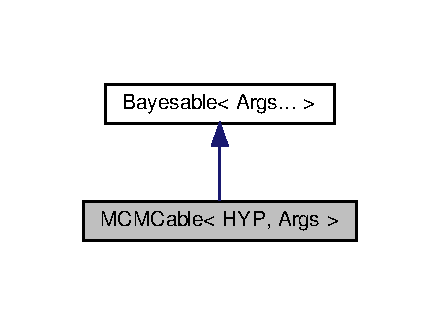
\includegraphics[width=214pt]{class_m_c_m_cable__inherit__graph}
\end{center}
\end{figure}


Collaboration diagram for M\+C\+M\+Cable$<$ this\+\_\+t, Args $>$\+:
\nopagebreak
\begin{figure}[H]
\begin{center}
\leavevmode
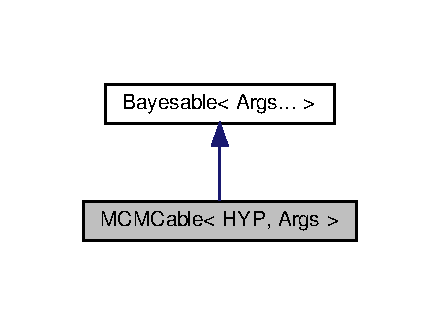
\includegraphics[width=214pt]{class_m_c_m_cable__coll__graph}
\end{center}
\end{figure}
\doxysubsection*{Public Member Functions}
\begin{DoxyCompactItemize}
\item 
\mbox{\hyperlink{class_m_c_m_cable_a3bc2cc7dd7cf2385ade7c82a51f3a566}{M\+C\+M\+Cable}} ()
\item 
virtual std\+::pair$<$ this\+\_\+t, double $>$ \mbox{\hyperlink{class_m_c_m_cable_a98b52f1867ea0d72c1c91b4496d756d2}{propose}} () const =0
\item 
virtual this\+\_\+t \mbox{\hyperlink{class_m_c_m_cable_aa7017e18b4a1508bc4cff90fb82a8ec1}{restart}} () const =0
\item 
virtual bool \mbox{\hyperlink{class_m_c_m_cable_a7b35c04d3d1326b930cfc69dfe0bd207}{operator==}} (const this\+\_\+t \&h) const =0
\item 
virtual bool \mbox{\hyperlink{class_m_c_m_cable_a73f816785855f80f5d102528aa671f4b}{operator!=}} (const this\+\_\+t \&h) const
\end{DoxyCompactItemize}
\doxysubsection*{Static Public Member Functions}
\begin{DoxyCompactItemize}
\item 
static this\+\_\+t \mbox{\hyperlink{class_m_c_m_cable_a376572ac482cac6d5352f45dbfefcb51}{sample}} ()
\begin{DoxyCompactList}\small\item\em Static function for making a hypothesis. Be careful using this with references because they may not foward right (for reasons that are unclear to me) \end{DoxyCompactList}\end{DoxyCompactItemize}
\doxysubsection*{Additional Inherited Members}


\doxysubsection{Detailed Description}
\subsubsection*{template$<$typename this\+\_\+t, typename... Args$>$\newline
class M\+C\+M\+Cable$<$ this\+\_\+t, Args $>$}

\begin{DoxyAuthor}{Author}
steven piantadosi 
\end{DoxyAuthor}
\begin{DoxyDate}{Date}
03/02/20 
\end{DoxyDate}


\doxysubsection{Constructor \& Destructor Documentation}
\mbox{\Hypertarget{class_m_c_m_cable_a3bc2cc7dd7cf2385ade7c82a51f3a566}\label{class_m_c_m_cable_a3bc2cc7dd7cf2385ade7c82a51f3a566}} 
\index{MCMCable$<$ this\_t, Args $>$@{MCMCable$<$ this\_t, Args $>$}!MCMCable@{MCMCable}}
\index{MCMCable@{MCMCable}!MCMCable$<$ this\_t, Args $>$@{MCMCable$<$ this\_t, Args $>$}}
\doxysubsubsection{\texorpdfstring{MCMCable()}{MCMCable()}}
{\footnotesize\ttfamily template$<$typename this\+\_\+t , typename... Args$>$ \\
\mbox{\hyperlink{class_m_c_m_cable}{M\+C\+M\+Cable}}$<$ this\+\_\+t, Args $>$\+::\mbox{\hyperlink{class_m_c_m_cable}{M\+C\+M\+Cable}} (\begin{DoxyParamCaption}{ }\end{DoxyParamCaption})\hspace{0.3cm}{\ttfamily [inline]}}



\doxysubsection{Member Function Documentation}
\mbox{\Hypertarget{class_m_c_m_cable_a73f816785855f80f5d102528aa671f4b}\label{class_m_c_m_cable_a73f816785855f80f5d102528aa671f4b}} 
\index{MCMCable$<$ this\_t, Args $>$@{MCMCable$<$ this\_t, Args $>$}!operator"!=@{operator"!=}}
\index{operator"!=@{operator"!=}!MCMCable$<$ this\_t, Args $>$@{MCMCable$<$ this\_t, Args $>$}}
\doxysubsubsection{\texorpdfstring{operator"!=()}{operator!=()}}
{\footnotesize\ttfamily template$<$typename this\+\_\+t , typename... Args$>$ \\
virtual bool \mbox{\hyperlink{class_m_c_m_cable}{M\+C\+M\+Cable}}$<$ this\+\_\+t, Args $>$\+::operator!= (\begin{DoxyParamCaption}\item[{const this\+\_\+t \&}]{h }\end{DoxyParamCaption}) const\hspace{0.3cm}{\ttfamily [inline]}, {\ttfamily [virtual]}}

\mbox{\Hypertarget{class_m_c_m_cable_a7b35c04d3d1326b930cfc69dfe0bd207}\label{class_m_c_m_cable_a7b35c04d3d1326b930cfc69dfe0bd207}} 
\index{MCMCable$<$ this\_t, Args $>$@{MCMCable$<$ this\_t, Args $>$}!operator==@{operator==}}
\index{operator==@{operator==}!MCMCable$<$ this\_t, Args $>$@{MCMCable$<$ this\_t, Args $>$}}
\doxysubsubsection{\texorpdfstring{operator==()}{operator==()}}
{\footnotesize\ttfamily template$<$typename this\+\_\+t , typename... Args$>$ \\
virtual bool \mbox{\hyperlink{class_m_c_m_cable}{M\+C\+M\+Cable}}$<$ this\+\_\+t, Args $>$\+::operator== (\begin{DoxyParamCaption}\item[{const this\+\_\+t \&}]{h }\end{DoxyParamCaption}) const\hspace{0.3cm}{\ttfamily [pure virtual]}}



Implemented in \mbox{\hyperlink{class_lexicon_a7623a6f5ad5156789088e461dbe9d2f6}{Lexicon$<$ this\+\_\+t, key\+\_\+t, I\+N\+N\+E\+R, \+\_\+input\+\_\+t, \+\_\+output\+\_\+t, datum\+\_\+t, \+\_\+\+Virtual\+Machine\+State\+\_\+t $>$}}, \mbox{\hyperlink{class_grammar_hypothesis_a5af8ece466cdc1d0fc2a960ae1d63462}{Grammar\+Hypothesis$<$ this\+\_\+t, \+\_\+\+H\+Y\+P, datum\+\_\+t, data\+\_\+t $>$}}, \mbox{\hyperlink{class_l_o_t_hypothesis_aab4eec5c502d4a3c11c93a81975fcde0}{L\+O\+T\+Hypothesis$<$ this\+\_\+t, \+\_\+input\+\_\+t, \+\_\+output\+\_\+t, \+\_\+\+Grammar\+\_\+t, grammar, \+\_\+datum\+\_\+t, \+\_\+data\+\_\+t, \+\_\+\+Virtual\+Machine\+State\+\_\+t $>$}}, \mbox{\hyperlink{class_vector_half_normal_hypothesis_ad6c4a4f67f0b53f35132295c00bedb2f}{Vector\+Half\+Normal\+Hypothesis}}, \mbox{\hyperlink{class_vector_normal_hypothesis_aabe2e0f4c86e52c04add65a55a046b6a}{Vector\+Normal\+Hypothesis}}, \mbox{\hyperlink{class_t_normal_variable_add62dd259e5d400ce6711f11e3e77455}{T\+Normal\+Variable$<$ f $>$}}, and \mbox{\hyperlink{class_t_normal_variable_add62dd259e5d400ce6711f11e3e77455}{T\+Normal\+Variable$<$+\mbox{[}$\,$\mbox{]}(float x) -\/$>$}}.

\mbox{\Hypertarget{class_m_c_m_cable_a98b52f1867ea0d72c1c91b4496d756d2}\label{class_m_c_m_cable_a98b52f1867ea0d72c1c91b4496d756d2}} 
\index{MCMCable$<$ this\_t, Args $>$@{MCMCable$<$ this\_t, Args $>$}!propose@{propose}}
\index{propose@{propose}!MCMCable$<$ this\_t, Args $>$@{MCMCable$<$ this\_t, Args $>$}}
\doxysubsubsection{\texorpdfstring{propose()}{propose()}}
{\footnotesize\ttfamily template$<$typename this\+\_\+t , typename... Args$>$ \\
virtual std\+::pair$<$this\+\_\+t,double$>$ \mbox{\hyperlink{class_m_c_m_cable}{M\+C\+M\+Cable}}$<$ this\+\_\+t, Args $>$\+::propose (\begin{DoxyParamCaption}{ }\end{DoxyParamCaption}) const\hspace{0.3cm}{\ttfamily [pure virtual]}}



Implemented in \mbox{\hyperlink{class_t_normal_variable_ad749023d34d2fad8b465aa2bfeba51a3}{T\+Normal\+Variable$<$+\mbox{[}$\,$\mbox{]}(float x) -\/$>$}}.

\mbox{\Hypertarget{class_m_c_m_cable_aa7017e18b4a1508bc4cff90fb82a8ec1}\label{class_m_c_m_cable_aa7017e18b4a1508bc4cff90fb82a8ec1}} 
\index{MCMCable$<$ this\_t, Args $>$@{MCMCable$<$ this\_t, Args $>$}!restart@{restart}}
\index{restart@{restart}!MCMCable$<$ this\_t, Args $>$@{MCMCable$<$ this\_t, Args $>$}}
\doxysubsubsection{\texorpdfstring{restart()}{restart()}}
{\footnotesize\ttfamily template$<$typename this\+\_\+t , typename... Args$>$ \\
virtual this\+\_\+t \mbox{\hyperlink{class_m_c_m_cable}{M\+C\+M\+Cable}}$<$ this\+\_\+t, Args $>$\+::restart (\begin{DoxyParamCaption}{ }\end{DoxyParamCaption}) const\hspace{0.3cm}{\ttfamily [pure virtual]}}



Implemented in \mbox{\hyperlink{class_t_normal_variable_aacaa3c0962cf32dcee93f7e459cd0eac}{T\+Normal\+Variable$<$+\mbox{[}$\,$\mbox{]}(float x) -\/$>$}}.

\mbox{\Hypertarget{class_m_c_m_cable_a376572ac482cac6d5352f45dbfefcb51}\label{class_m_c_m_cable_a376572ac482cac6d5352f45dbfefcb51}} 
\index{MCMCable$<$ this\_t, Args $>$@{MCMCable$<$ this\_t, Args $>$}!sample@{sample}}
\index{sample@{sample}!MCMCable$<$ this\_t, Args $>$@{MCMCable$<$ this\_t, Args $>$}}
\doxysubsubsection{\texorpdfstring{sample()}{sample()}}
{\footnotesize\ttfamily template$<$typename this\+\_\+t , typename... Args$>$ \\
static this\+\_\+t \mbox{\hyperlink{class_m_c_m_cable}{M\+C\+M\+Cable}}$<$ this\+\_\+t, Args $>$\+::sample (\begin{DoxyParamCaption}{ }\end{DoxyParamCaption})\hspace{0.3cm}{\ttfamily [inline]}, {\ttfamily [static]}}



Static function for making a hypothesis. Be careful using this with references because they may not foward right (for reasons that are unclear to me) 

\begin{DoxyReturn}{Returns}

\end{DoxyReturn}


The documentation for this class was generated from the following file\+:\begin{DoxyCompactItemize}
\item 
src/\+Hypotheses/\+Interfaces/\mbox{\hyperlink{_m_c_m_cable_8h}{M\+C\+M\+Cable.\+h}}\end{DoxyCompactItemize}

\hypertarget{class_m_c_m_c_chain}{}\section{M\+C\+M\+C\+Chain$<$ H\+YP, callback\+\_\+t $>$ Class Template Reference}
\label{class_m_c_m_c_chain}\index{M\+C\+M\+C\+Chain$<$ H\+Y\+P, callback\+\_\+t $>$@{M\+C\+M\+C\+Chain$<$ H\+Y\+P, callback\+\_\+t $>$}}


{\ttfamily \#include $<$M\+C\+M\+C\+Chain.\+h$>$}



Collaboration diagram for M\+C\+M\+C\+Chain$<$ H\+YP, callback\+\_\+t $>$\+:
\nopagebreak
\begin{figure}[H]
\begin{center}
\leavevmode
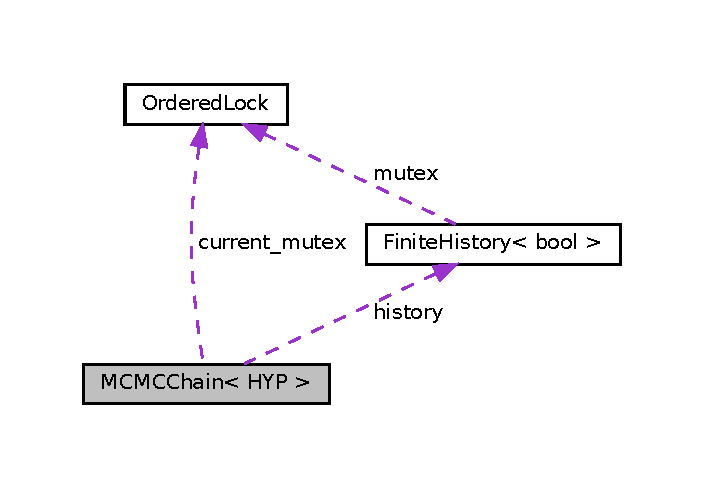
\includegraphics[width=243pt]{class_m_c_m_c_chain__coll__graph}
\end{center}
\end{figure}
\subsection*{Public Member Functions}
\begin{DoxyCompactItemize}
\item 
\hyperlink{class_m_c_m_c_chain_aed5ffea5a46a380b8b0d78cd46c96a97}{M\+C\+M\+C\+Chain} (H\+YP \&h0, typename H\+Y\+P\+::data\+\_\+t $\ast$d, callback\+\_\+t \&cb)
\item 
\hyperlink{class_m_c_m_c_chain_a731f2ca6416f1daa84cd54cd3f9281b2}{M\+C\+M\+C\+Chain} (H\+YP \&\&h0, typename H\+Y\+P\+::data\+\_\+t $\ast$d, callback\+\_\+t \&cb)
\item 
\hyperlink{class_m_c_m_c_chain_afaa9a75b515252a8c6237aad0211a2f2}{M\+C\+M\+C\+Chain} (H\+YP \&h0, typename H\+Y\+P\+::data\+\_\+t $\ast$d, callback\+\_\+t $\ast$cb=nullptr)
\item 
\hyperlink{class_m_c_m_c_chain_a8df81470759ddd5654c5a82ad3b185cf}{M\+C\+M\+C\+Chain} (H\+YP \&\&h0, typename H\+Y\+P\+::data\+\_\+t $\ast$d, callback\+\_\+t $\ast$cb=nullptr)
\item 
\hyperlink{class_m_c_m_c_chain_a3942ff362dcc0bdfdad296f95048f14e}{M\+C\+M\+C\+Chain} (const \hyperlink{class_m_c_m_c_chain}{M\+C\+M\+C\+Chain} \&m)
\item 
\hyperlink{class_m_c_m_c_chain_a2db84c6b92af066b34eedd257d800417}{M\+C\+M\+C\+Chain} (\hyperlink{class_m_c_m_c_chain}{M\+C\+M\+C\+Chain} \&\&m)
\item 
virtual \hyperlink{class_m_c_m_c_chain_ad19438dd99bdba43b5175705e2bef156}{$\sim$\+M\+C\+M\+C\+Chain} ()
\item 
H\+YP \& \hyperlink{class_m_c_m_c_chain_ae76c66b5bcbc02df926e5f9a91acff17}{get\+Current} ()
\item 
void \hyperlink{class_m_c_m_c_chain_a4214114e0ef4adcd4badfe1440693190}{run\+On\+Current} ()
\item 
const H\+YP \& \hyperlink{class_m_c_m_c_chain_aa5c2bf3cae9a5959cab43e04b1201ed2}{get\+Max} ()
\item 
void \hyperlink{class_m_c_m_c_chain_aef30134b1915b8b494040771480d6b80}{run} (\hyperlink{struct_control}{Control} ctl)
\item 
void \hyperlink{class_m_c_m_c_chain_ae59e07a79da1bf56b01429efcb9fb312}{run} ()
\item 
double \hyperlink{class_m_c_m_c_chain_a4b2b8b51e5ba868bca024f2be737e4c6}{acceptance\+\_\+ratio} ()
\item 
double \hyperlink{class_m_c_m_c_chain_a9adc3d08662ad7035cc9d9d75a1fc5a6}{at\+\_\+temperature} (double t)
\end{DoxyCompactItemize}
\subsection*{Public Attributes}
\begin{DoxyCompactItemize}
\item 
H\+YP \hyperlink{class_m_c_m_c_chain_ab0c3b31e96d1f703bb8cf55c0575b4bd}{current}
\item 
std\+::mutex \hyperlink{class_m_c_m_c_chain_a42c355121fce0476426a49d5498c38a1}{current\+\_\+mutex}
\item 
H\+Y\+P\+::data\+\_\+t $\ast$ \hyperlink{class_m_c_m_c_chain_ab235f08fad93a9626ffb566c001ed5c9}{data}
\item 
double \hyperlink{class_m_c_m_c_chain_a3b8d31f47d75503321b432eeac0bb13b}{maxval}
\item 
callback\+\_\+t $\ast$ \hyperlink{class_m_c_m_c_chain_aa7a4a0d46ae2d9818c2f076f839badd7}{callback}
\item 
unsigned long \hyperlink{class_m_c_m_c_chain_a0d3ac649b04077cd0ffea236df560c91}{samples}
\item 
unsigned long \hyperlink{class_m_c_m_c_chain_aec2cdd6a3e25447c7f34e31d0d98dbcb}{proposals}
\item 
unsigned long \hyperlink{class_m_c_m_c_chain_ae1597e42074b2efb93ace3e40f1f7a45}{acceptances}
\item 
unsigned long \hyperlink{class_m_c_m_c_chain_aeac1cd63d13c397ba01cca35b605b786}{steps\+\_\+since\+\_\+improvement}
\item 
std\+::atomic$<$ double $>$ \hyperlink{class_m_c_m_c_chain_a7173287e1c0e681a9912a84c87320ece}{temperature}
\item 
\hyperlink{class_finite_history}{Finite\+History}$<$ bool $>$ \hyperlink{class_m_c_m_c_chain_a83cb52eb26bdb914c0eb483f541972a9}{history}
\end{DoxyCompactItemize}


\subsection{Constructor \& Destructor Documentation}
\mbox{\Hypertarget{class_m_c_m_c_chain_aed5ffea5a46a380b8b0d78cd46c96a97}\label{class_m_c_m_c_chain_aed5ffea5a46a380b8b0d78cd46c96a97}} 
\index{M\+C\+M\+C\+Chain@{M\+C\+M\+C\+Chain}!M\+C\+M\+C\+Chain@{M\+C\+M\+C\+Chain}}
\index{M\+C\+M\+C\+Chain@{M\+C\+M\+C\+Chain}!M\+C\+M\+C\+Chain@{M\+C\+M\+C\+Chain}}
\subsubsection{\texorpdfstring{M\+C\+M\+C\+Chain()}{MCMCChain()}\hspace{0.1cm}{\footnotesize\ttfamily [1/6]}}
{\footnotesize\ttfamily template$<$typename H\+YP , typename callback\+\_\+t $>$ \\
\hyperlink{class_m_c_m_c_chain}{M\+C\+M\+C\+Chain}$<$ H\+YP, callback\+\_\+t $>$\+::\hyperlink{class_m_c_m_c_chain}{M\+C\+M\+C\+Chain} (\begin{DoxyParamCaption}\item[{H\+YP \&}]{h0,  }\item[{typename H\+Y\+P\+::data\+\_\+t $\ast$}]{d,  }\item[{callback\+\_\+t \&}]{cb }\end{DoxyParamCaption})\hspace{0.3cm}{\ttfamily [inline]}}

\mbox{\Hypertarget{class_m_c_m_c_chain_a731f2ca6416f1daa84cd54cd3f9281b2}\label{class_m_c_m_c_chain_a731f2ca6416f1daa84cd54cd3f9281b2}} 
\index{M\+C\+M\+C\+Chain@{M\+C\+M\+C\+Chain}!M\+C\+M\+C\+Chain@{M\+C\+M\+C\+Chain}}
\index{M\+C\+M\+C\+Chain@{M\+C\+M\+C\+Chain}!M\+C\+M\+C\+Chain@{M\+C\+M\+C\+Chain}}
\subsubsection{\texorpdfstring{M\+C\+M\+C\+Chain()}{MCMCChain()}\hspace{0.1cm}{\footnotesize\ttfamily [2/6]}}
{\footnotesize\ttfamily template$<$typename H\+YP , typename callback\+\_\+t $>$ \\
\hyperlink{class_m_c_m_c_chain}{M\+C\+M\+C\+Chain}$<$ H\+YP, callback\+\_\+t $>$\+::\hyperlink{class_m_c_m_c_chain}{M\+C\+M\+C\+Chain} (\begin{DoxyParamCaption}\item[{H\+YP \&\&}]{h0,  }\item[{typename H\+Y\+P\+::data\+\_\+t $\ast$}]{d,  }\item[{callback\+\_\+t \&}]{cb }\end{DoxyParamCaption})\hspace{0.3cm}{\ttfamily [inline]}}

\mbox{\Hypertarget{class_m_c_m_c_chain_afaa9a75b515252a8c6237aad0211a2f2}\label{class_m_c_m_c_chain_afaa9a75b515252a8c6237aad0211a2f2}} 
\index{M\+C\+M\+C\+Chain@{M\+C\+M\+C\+Chain}!M\+C\+M\+C\+Chain@{M\+C\+M\+C\+Chain}}
\index{M\+C\+M\+C\+Chain@{M\+C\+M\+C\+Chain}!M\+C\+M\+C\+Chain@{M\+C\+M\+C\+Chain}}
\subsubsection{\texorpdfstring{M\+C\+M\+C\+Chain()}{MCMCChain()}\hspace{0.1cm}{\footnotesize\ttfamily [3/6]}}
{\footnotesize\ttfamily template$<$typename H\+YP , typename callback\+\_\+t $>$ \\
\hyperlink{class_m_c_m_c_chain}{M\+C\+M\+C\+Chain}$<$ H\+YP, callback\+\_\+t $>$\+::\hyperlink{class_m_c_m_c_chain}{M\+C\+M\+C\+Chain} (\begin{DoxyParamCaption}\item[{H\+YP \&}]{h0,  }\item[{typename H\+Y\+P\+::data\+\_\+t $\ast$}]{d,  }\item[{callback\+\_\+t $\ast$}]{cb = {\ttfamily nullptr} }\end{DoxyParamCaption})\hspace{0.3cm}{\ttfamily [inline]}}

\mbox{\Hypertarget{class_m_c_m_c_chain_a8df81470759ddd5654c5a82ad3b185cf}\label{class_m_c_m_c_chain_a8df81470759ddd5654c5a82ad3b185cf}} 
\index{M\+C\+M\+C\+Chain@{M\+C\+M\+C\+Chain}!M\+C\+M\+C\+Chain@{M\+C\+M\+C\+Chain}}
\index{M\+C\+M\+C\+Chain@{M\+C\+M\+C\+Chain}!M\+C\+M\+C\+Chain@{M\+C\+M\+C\+Chain}}
\subsubsection{\texorpdfstring{M\+C\+M\+C\+Chain()}{MCMCChain()}\hspace{0.1cm}{\footnotesize\ttfamily [4/6]}}
{\footnotesize\ttfamily template$<$typename H\+YP , typename callback\+\_\+t $>$ \\
\hyperlink{class_m_c_m_c_chain}{M\+C\+M\+C\+Chain}$<$ H\+YP, callback\+\_\+t $>$\+::\hyperlink{class_m_c_m_c_chain}{M\+C\+M\+C\+Chain} (\begin{DoxyParamCaption}\item[{H\+YP \&\&}]{h0,  }\item[{typename H\+Y\+P\+::data\+\_\+t $\ast$}]{d,  }\item[{callback\+\_\+t $\ast$}]{cb = {\ttfamily nullptr} }\end{DoxyParamCaption})\hspace{0.3cm}{\ttfamily [inline]}}

\mbox{\Hypertarget{class_m_c_m_c_chain_a3942ff362dcc0bdfdad296f95048f14e}\label{class_m_c_m_c_chain_a3942ff362dcc0bdfdad296f95048f14e}} 
\index{M\+C\+M\+C\+Chain@{M\+C\+M\+C\+Chain}!M\+C\+M\+C\+Chain@{M\+C\+M\+C\+Chain}}
\index{M\+C\+M\+C\+Chain@{M\+C\+M\+C\+Chain}!M\+C\+M\+C\+Chain@{M\+C\+M\+C\+Chain}}
\subsubsection{\texorpdfstring{M\+C\+M\+C\+Chain()}{MCMCChain()}\hspace{0.1cm}{\footnotesize\ttfamily [5/6]}}
{\footnotesize\ttfamily template$<$typename H\+YP , typename callback\+\_\+t $>$ \\
\hyperlink{class_m_c_m_c_chain}{M\+C\+M\+C\+Chain}$<$ H\+YP, callback\+\_\+t $>$\+::\hyperlink{class_m_c_m_c_chain}{M\+C\+M\+C\+Chain} (\begin{DoxyParamCaption}\item[{const \hyperlink{class_m_c_m_c_chain}{M\+C\+M\+C\+Chain}$<$ H\+YP, callback\+\_\+t $>$ \&}]{m }\end{DoxyParamCaption})\hspace{0.3cm}{\ttfamily [inline]}}

\mbox{\Hypertarget{class_m_c_m_c_chain_a2db84c6b92af066b34eedd257d800417}\label{class_m_c_m_c_chain_a2db84c6b92af066b34eedd257d800417}} 
\index{M\+C\+M\+C\+Chain@{M\+C\+M\+C\+Chain}!M\+C\+M\+C\+Chain@{M\+C\+M\+C\+Chain}}
\index{M\+C\+M\+C\+Chain@{M\+C\+M\+C\+Chain}!M\+C\+M\+C\+Chain@{M\+C\+M\+C\+Chain}}
\subsubsection{\texorpdfstring{M\+C\+M\+C\+Chain()}{MCMCChain()}\hspace{0.1cm}{\footnotesize\ttfamily [6/6]}}
{\footnotesize\ttfamily template$<$typename H\+YP , typename callback\+\_\+t $>$ \\
\hyperlink{class_m_c_m_c_chain}{M\+C\+M\+C\+Chain}$<$ H\+YP, callback\+\_\+t $>$\+::\hyperlink{class_m_c_m_c_chain}{M\+C\+M\+C\+Chain} (\begin{DoxyParamCaption}\item[{\hyperlink{class_m_c_m_c_chain}{M\+C\+M\+C\+Chain}$<$ H\+YP, callback\+\_\+t $>$ \&\&}]{m }\end{DoxyParamCaption})\hspace{0.3cm}{\ttfamily [inline]}}

\mbox{\Hypertarget{class_m_c_m_c_chain_ad19438dd99bdba43b5175705e2bef156}\label{class_m_c_m_c_chain_ad19438dd99bdba43b5175705e2bef156}} 
\index{M\+C\+M\+C\+Chain@{M\+C\+M\+C\+Chain}!````~M\+C\+M\+C\+Chain@{$\sim$\+M\+C\+M\+C\+Chain}}
\index{````~M\+C\+M\+C\+Chain@{$\sim$\+M\+C\+M\+C\+Chain}!M\+C\+M\+C\+Chain@{M\+C\+M\+C\+Chain}}
\subsubsection{\texorpdfstring{$\sim$\+M\+C\+M\+C\+Chain()}{~MCMCChain()}}
{\footnotesize\ttfamily template$<$typename H\+YP , typename callback\+\_\+t $>$ \\
virtual \hyperlink{class_m_c_m_c_chain}{M\+C\+M\+C\+Chain}$<$ H\+YP, callback\+\_\+t $>$\+::$\sim$\hyperlink{class_m_c_m_c_chain}{M\+C\+M\+C\+Chain} (\begin{DoxyParamCaption}{ }\end{DoxyParamCaption})\hspace{0.3cm}{\ttfamily [inline]}, {\ttfamily [virtual]}}



\subsection{Member Function Documentation}
\mbox{\Hypertarget{class_m_c_m_c_chain_a4b2b8b51e5ba868bca024f2be737e4c6}\label{class_m_c_m_c_chain_a4b2b8b51e5ba868bca024f2be737e4c6}} 
\index{M\+C\+M\+C\+Chain@{M\+C\+M\+C\+Chain}!acceptance\+\_\+ratio@{acceptance\+\_\+ratio}}
\index{acceptance\+\_\+ratio@{acceptance\+\_\+ratio}!M\+C\+M\+C\+Chain@{M\+C\+M\+C\+Chain}}
\subsubsection{\texorpdfstring{acceptance\+\_\+ratio()}{acceptance\_ratio()}}
{\footnotesize\ttfamily template$<$typename H\+YP , typename callback\+\_\+t $>$ \\
double \hyperlink{class_m_c_m_c_chain}{M\+C\+M\+C\+Chain}$<$ H\+YP, callback\+\_\+t $>$\+::acceptance\+\_\+ratio (\begin{DoxyParamCaption}{ }\end{DoxyParamCaption})\hspace{0.3cm}{\ttfamily [inline]}}

Get my acceptance ratio \begin{DoxyReturn}{Returns}

\end{DoxyReturn}
\mbox{\Hypertarget{class_m_c_m_c_chain_a9adc3d08662ad7035cc9d9d75a1fc5a6}\label{class_m_c_m_c_chain_a9adc3d08662ad7035cc9d9d75a1fc5a6}} 
\index{M\+C\+M\+C\+Chain@{M\+C\+M\+C\+Chain}!at\+\_\+temperature@{at\+\_\+temperature}}
\index{at\+\_\+temperature@{at\+\_\+temperature}!M\+C\+M\+C\+Chain@{M\+C\+M\+C\+Chain}}
\subsubsection{\texorpdfstring{at\+\_\+temperature()}{at\_temperature()}}
{\footnotesize\ttfamily template$<$typename H\+YP , typename callback\+\_\+t $>$ \\
double \hyperlink{class_m_c_m_c_chain}{M\+C\+M\+C\+Chain}$<$ H\+YP, callback\+\_\+t $>$\+::at\+\_\+temperature (\begin{DoxyParamCaption}\item[{double}]{t }\end{DoxyParamCaption})\hspace{0.3cm}{\ttfamily [inline]}}

Return my current posterior at a given temperature t 
\begin{DoxyParams}{Parameters}
{\em t} & \\
\hline
\end{DoxyParams}
\begin{DoxyReturn}{Returns}

\end{DoxyReturn}
\mbox{\Hypertarget{class_m_c_m_c_chain_ae76c66b5bcbc02df926e5f9a91acff17}\label{class_m_c_m_c_chain_ae76c66b5bcbc02df926e5f9a91acff17}} 
\index{M\+C\+M\+C\+Chain@{M\+C\+M\+C\+Chain}!get\+Current@{get\+Current}}
\index{get\+Current@{get\+Current}!M\+C\+M\+C\+Chain@{M\+C\+M\+C\+Chain}}
\subsubsection{\texorpdfstring{get\+Current()}{getCurrent()}}
{\footnotesize\ttfamily template$<$typename H\+YP , typename callback\+\_\+t $>$ \\
H\+YP\& \hyperlink{class_m_c_m_c_chain}{M\+C\+M\+C\+Chain}$<$ H\+YP, callback\+\_\+t $>$\+::get\+Current (\begin{DoxyParamCaption}{ }\end{DoxyParamCaption})\hspace{0.3cm}{\ttfamily [inline]}}

get a reference to the current value \begin{DoxyReturn}{Returns}

\end{DoxyReturn}
\mbox{\Hypertarget{class_m_c_m_c_chain_aa5c2bf3cae9a5959cab43e04b1201ed2}\label{class_m_c_m_c_chain_aa5c2bf3cae9a5959cab43e04b1201ed2}} 
\index{M\+C\+M\+C\+Chain@{M\+C\+M\+C\+Chain}!get\+Max@{get\+Max}}
\index{get\+Max@{get\+Max}!M\+C\+M\+C\+Chain@{M\+C\+M\+C\+Chain}}
\subsubsection{\texorpdfstring{get\+Max()}{getMax()}}
{\footnotesize\ttfamily template$<$typename H\+YP , typename callback\+\_\+t $>$ \\
const H\+YP\& \hyperlink{class_m_c_m_c_chain}{M\+C\+M\+C\+Chain}$<$ H\+YP, callback\+\_\+t $>$\+::get\+Max (\begin{DoxyParamCaption}{ }\end{DoxyParamCaption})\hspace{0.3cm}{\ttfamily [inline]}}

\mbox{\Hypertarget{class_m_c_m_c_chain_aef30134b1915b8b494040771480d6b80}\label{class_m_c_m_c_chain_aef30134b1915b8b494040771480d6b80}} 
\index{M\+C\+M\+C\+Chain@{M\+C\+M\+C\+Chain}!run@{run}}
\index{run@{run}!M\+C\+M\+C\+Chain@{M\+C\+M\+C\+Chain}}
\subsubsection{\texorpdfstring{run()}{run()}\hspace{0.1cm}{\footnotesize\ttfamily [1/2]}}
{\footnotesize\ttfamily template$<$typename H\+YP , typename callback\+\_\+t $>$ \\
void \hyperlink{class_m_c_m_c_chain}{M\+C\+M\+C\+Chain}$<$ H\+YP, callback\+\_\+t $>$\+::run (\begin{DoxyParamCaption}\item[{\hyperlink{struct_control}{Control}}]{ctl }\end{DoxyParamCaption})\hspace{0.3cm}{\ttfamily [inline]}}

Run M\+C\+MC according to the control parameters passed in. N\+O\+TE\+: ctl cannot be passed by reference. 
\begin{DoxyParams}{Parameters}
{\em ctl} & \\
\hline
\end{DoxyParams}
\mbox{\Hypertarget{class_m_c_m_c_chain_ae59e07a79da1bf56b01429efcb9fb312}\label{class_m_c_m_c_chain_ae59e07a79da1bf56b01429efcb9fb312}} 
\index{M\+C\+M\+C\+Chain@{M\+C\+M\+C\+Chain}!run@{run}}
\index{run@{run}!M\+C\+M\+C\+Chain@{M\+C\+M\+C\+Chain}}
\subsubsection{\texorpdfstring{run()}{run()}\hspace{0.1cm}{\footnotesize\ttfamily [2/2]}}
{\footnotesize\ttfamily template$<$typename H\+YP , typename callback\+\_\+t $>$ \\
void \hyperlink{class_m_c_m_c_chain}{M\+C\+M\+C\+Chain}$<$ H\+YP, callback\+\_\+t $>$\+::run (\begin{DoxyParamCaption}{ }\end{DoxyParamCaption})\hspace{0.3cm}{\ttfamily [inline]}}

Run forever\mbox{\Hypertarget{class_m_c_m_c_chain_a4214114e0ef4adcd4badfe1440693190}\label{class_m_c_m_c_chain_a4214114e0ef4adcd4badfe1440693190}} 
\index{M\+C\+M\+C\+Chain@{M\+C\+M\+C\+Chain}!run\+On\+Current@{run\+On\+Current}}
\index{run\+On\+Current@{run\+On\+Current}!M\+C\+M\+C\+Chain@{M\+C\+M\+C\+Chain}}
\subsubsection{\texorpdfstring{run\+On\+Current()}{runOnCurrent()}}
{\footnotesize\ttfamily template$<$typename H\+YP , typename callback\+\_\+t $>$ \\
void \hyperlink{class_m_c_m_c_chain}{M\+C\+M\+C\+Chain}$<$ H\+YP, callback\+\_\+t $>$\+::run\+On\+Current (\begin{DoxyParamCaption}{ }\end{DoxyParamCaption})\hspace{0.3cm}{\ttfamily [inline]}}

This is called by the constructor to compute the posterior and callback for an initial h0

\subsection{Member Data Documentation}
\mbox{\Hypertarget{class_m_c_m_c_chain_ae1597e42074b2efb93ace3e40f1f7a45}\label{class_m_c_m_c_chain_ae1597e42074b2efb93ace3e40f1f7a45}} 
\index{M\+C\+M\+C\+Chain@{M\+C\+M\+C\+Chain}!acceptances@{acceptances}}
\index{acceptances@{acceptances}!M\+C\+M\+C\+Chain@{M\+C\+M\+C\+Chain}}
\subsubsection{\texorpdfstring{acceptances}{acceptances}}
{\footnotesize\ttfamily template$<$typename H\+YP , typename callback\+\_\+t $>$ \\
unsigned long \hyperlink{class_m_c_m_c_chain}{M\+C\+M\+C\+Chain}$<$ H\+YP, callback\+\_\+t $>$\+::acceptances}

\mbox{\Hypertarget{class_m_c_m_c_chain_aa7a4a0d46ae2d9818c2f076f839badd7}\label{class_m_c_m_c_chain_aa7a4a0d46ae2d9818c2f076f839badd7}} 
\index{M\+C\+M\+C\+Chain@{M\+C\+M\+C\+Chain}!callback@{callback}}
\index{callback@{callback}!M\+C\+M\+C\+Chain@{M\+C\+M\+C\+Chain}}
\subsubsection{\texorpdfstring{callback}{callback}}
{\footnotesize\ttfamily template$<$typename H\+YP , typename callback\+\_\+t $>$ \\
callback\+\_\+t$\ast$ \hyperlink{class_m_c_m_c_chain}{M\+C\+M\+C\+Chain}$<$ H\+YP, callback\+\_\+t $>$\+::callback}

\mbox{\Hypertarget{class_m_c_m_c_chain_ab0c3b31e96d1f703bb8cf55c0575b4bd}\label{class_m_c_m_c_chain_ab0c3b31e96d1f703bb8cf55c0575b4bd}} 
\index{M\+C\+M\+C\+Chain@{M\+C\+M\+C\+Chain}!current@{current}}
\index{current@{current}!M\+C\+M\+C\+Chain@{M\+C\+M\+C\+Chain}}
\subsubsection{\texorpdfstring{current}{current}}
{\footnotesize\ttfamily template$<$typename H\+YP , typename callback\+\_\+t $>$ \\
H\+YP \hyperlink{class_m_c_m_c_chain}{M\+C\+M\+C\+Chain}$<$ H\+YP, callback\+\_\+t $>$\+::current}

\mbox{\Hypertarget{class_m_c_m_c_chain_a42c355121fce0476426a49d5498c38a1}\label{class_m_c_m_c_chain_a42c355121fce0476426a49d5498c38a1}} 
\index{M\+C\+M\+C\+Chain@{M\+C\+M\+C\+Chain}!current\+\_\+mutex@{current\+\_\+mutex}}
\index{current\+\_\+mutex@{current\+\_\+mutex}!M\+C\+M\+C\+Chain@{M\+C\+M\+C\+Chain}}
\subsubsection{\texorpdfstring{current\+\_\+mutex}{current\_mutex}}
{\footnotesize\ttfamily template$<$typename H\+YP , typename callback\+\_\+t $>$ \\
std\+::mutex \hyperlink{class_m_c_m_c_chain}{M\+C\+M\+C\+Chain}$<$ H\+YP, callback\+\_\+t $>$\+::current\+\_\+mutex\hspace{0.3cm}{\ttfamily [mutable]}}

\mbox{\Hypertarget{class_m_c_m_c_chain_ab235f08fad93a9626ffb566c001ed5c9}\label{class_m_c_m_c_chain_ab235f08fad93a9626ffb566c001ed5c9}} 
\index{M\+C\+M\+C\+Chain@{M\+C\+M\+C\+Chain}!data@{data}}
\index{data@{data}!M\+C\+M\+C\+Chain@{M\+C\+M\+C\+Chain}}
\subsubsection{\texorpdfstring{data}{data}}
{\footnotesize\ttfamily template$<$typename H\+YP , typename callback\+\_\+t $>$ \\
H\+Y\+P\+::data\+\_\+t$\ast$ \hyperlink{class_m_c_m_c_chain}{M\+C\+M\+C\+Chain}$<$ H\+YP, callback\+\_\+t $>$\+::data}

\mbox{\Hypertarget{class_m_c_m_c_chain_a83cb52eb26bdb914c0eb483f541972a9}\label{class_m_c_m_c_chain_a83cb52eb26bdb914c0eb483f541972a9}} 
\index{M\+C\+M\+C\+Chain@{M\+C\+M\+C\+Chain}!history@{history}}
\index{history@{history}!M\+C\+M\+C\+Chain@{M\+C\+M\+C\+Chain}}
\subsubsection{\texorpdfstring{history}{history}}
{\footnotesize\ttfamily template$<$typename H\+YP , typename callback\+\_\+t $>$ \\
\hyperlink{class_finite_history}{Finite\+History}$<$bool$>$ \hyperlink{class_m_c_m_c_chain}{M\+C\+M\+C\+Chain}$<$ H\+YP, callback\+\_\+t $>$\+::history}

\mbox{\Hypertarget{class_m_c_m_c_chain_a3b8d31f47d75503321b432eeac0bb13b}\label{class_m_c_m_c_chain_a3b8d31f47d75503321b432eeac0bb13b}} 
\index{M\+C\+M\+C\+Chain@{M\+C\+M\+C\+Chain}!maxval@{maxval}}
\index{maxval@{maxval}!M\+C\+M\+C\+Chain@{M\+C\+M\+C\+Chain}}
\subsubsection{\texorpdfstring{maxval}{maxval}}
{\footnotesize\ttfamily template$<$typename H\+YP , typename callback\+\_\+t $>$ \\
double \hyperlink{class_m_c_m_c_chain}{M\+C\+M\+C\+Chain}$<$ H\+YP, callback\+\_\+t $>$\+::maxval}

\mbox{\Hypertarget{class_m_c_m_c_chain_aec2cdd6a3e25447c7f34e31d0d98dbcb}\label{class_m_c_m_c_chain_aec2cdd6a3e25447c7f34e31d0d98dbcb}} 
\index{M\+C\+M\+C\+Chain@{M\+C\+M\+C\+Chain}!proposals@{proposals}}
\index{proposals@{proposals}!M\+C\+M\+C\+Chain@{M\+C\+M\+C\+Chain}}
\subsubsection{\texorpdfstring{proposals}{proposals}}
{\footnotesize\ttfamily template$<$typename H\+YP , typename callback\+\_\+t $>$ \\
unsigned long \hyperlink{class_m_c_m_c_chain}{M\+C\+M\+C\+Chain}$<$ H\+YP, callback\+\_\+t $>$\+::proposals}

\mbox{\Hypertarget{class_m_c_m_c_chain_a0d3ac649b04077cd0ffea236df560c91}\label{class_m_c_m_c_chain_a0d3ac649b04077cd0ffea236df560c91}} 
\index{M\+C\+M\+C\+Chain@{M\+C\+M\+C\+Chain}!samples@{samples}}
\index{samples@{samples}!M\+C\+M\+C\+Chain@{M\+C\+M\+C\+Chain}}
\subsubsection{\texorpdfstring{samples}{samples}}
{\footnotesize\ttfamily template$<$typename H\+YP , typename callback\+\_\+t $>$ \\
unsigned long \hyperlink{class_m_c_m_c_chain}{M\+C\+M\+C\+Chain}$<$ H\+YP, callback\+\_\+t $>$\+::samples}

\mbox{\Hypertarget{class_m_c_m_c_chain_aeac1cd63d13c397ba01cca35b605b786}\label{class_m_c_m_c_chain_aeac1cd63d13c397ba01cca35b605b786}} 
\index{M\+C\+M\+C\+Chain@{M\+C\+M\+C\+Chain}!steps\+\_\+since\+\_\+improvement@{steps\+\_\+since\+\_\+improvement}}
\index{steps\+\_\+since\+\_\+improvement@{steps\+\_\+since\+\_\+improvement}!M\+C\+M\+C\+Chain@{M\+C\+M\+C\+Chain}}
\subsubsection{\texorpdfstring{steps\+\_\+since\+\_\+improvement}{steps\_since\_improvement}}
{\footnotesize\ttfamily template$<$typename H\+YP , typename callback\+\_\+t $>$ \\
unsigned long \hyperlink{class_m_c_m_c_chain}{M\+C\+M\+C\+Chain}$<$ H\+YP, callback\+\_\+t $>$\+::steps\+\_\+since\+\_\+improvement}

\mbox{\Hypertarget{class_m_c_m_c_chain_a7173287e1c0e681a9912a84c87320ece}\label{class_m_c_m_c_chain_a7173287e1c0e681a9912a84c87320ece}} 
\index{M\+C\+M\+C\+Chain@{M\+C\+M\+C\+Chain}!temperature@{temperature}}
\index{temperature@{temperature}!M\+C\+M\+C\+Chain@{M\+C\+M\+C\+Chain}}
\subsubsection{\texorpdfstring{temperature}{temperature}}
{\footnotesize\ttfamily template$<$typename H\+YP , typename callback\+\_\+t $>$ \\
std\+::atomic$<$double$>$ \hyperlink{class_m_c_m_c_chain}{M\+C\+M\+C\+Chain}$<$ H\+YP, callback\+\_\+t $>$\+::temperature}



The documentation for this class was generated from the following file\+:\begin{DoxyCompactItemize}
\item 
src/\+Inference/\hyperlink{_m_c_m_c_chain_8h}{M\+C\+M\+C\+Chain.\+h}\end{DoxyCompactItemize}

\hypertarget{class_median_f_a_m_e}{}\section{Median\+F\+A\+ME$<$ T $>$ Class Template Reference}
\label{class_median_f_a_m_e}\index{Median\+F\+A\+M\+E$<$ T $>$@{Median\+F\+A\+M\+E$<$ T $>$}}


{\ttfamily \#include $<$Median\+F\+A\+M\+E.\+h$>$}



Collaboration diagram for Median\+F\+A\+ME$<$ T $>$\+:
\nopagebreak
\begin{figure}[H]
\begin{center}
\leavevmode
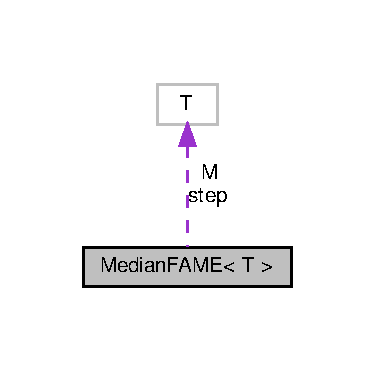
\includegraphics[width=180pt]{class_median_f_a_m_e__coll__graph}
\end{center}
\end{figure}
\subsection*{Public Member Functions}
\begin{DoxyCompactItemize}
\item 
\hyperlink{class_median_f_a_m_e_a5f7fa4a3764af4fbf6586479b3c2af46}{Median\+F\+A\+ME} ()
\item 
T \hyperlink{class_median_f_a_m_e_a3649461af2073421813b132f9f6e740b}{median} () const
\item 
void \hyperlink{class_median_f_a_m_e_aaf2310a3e21e455605c0f9d3375a7e5c}{add} (T x)
\item 
void \hyperlink{class_median_f_a_m_e_a95e83a1782a9fd3b79610a2c58a58dfe}{operator$<$$<$} (T x)
\end{DoxyCompactItemize}
\subsection*{Public Attributes}
\begin{DoxyCompactItemize}
\item 
T \hyperlink{class_median_f_a_m_e_a30154005cf17855ab19266f568803174}{M}
\item 
size\+\_\+t \hyperlink{class_median_f_a_m_e_a0318b43dd3ae39b735a152c16ae4baec}{n}
\item 
T \hyperlink{class_median_f_a_m_e_a99c7b975965259ed4079c08836583732}{step}
\end{DoxyCompactItemize}


\subsection{Detailed Description}
\subsubsection*{template$<$typename T$>$\newline
class Median\+F\+A\+M\+E$<$ T $>$}

\begin{DoxyAuthor}{Author}
steven piantadosi 
\end{DoxyAuthor}
\begin{DoxyDate}{Date}
03/02/20 
\end{DoxyDate}


\subsection{Constructor \& Destructor Documentation}
\mbox{\Hypertarget{class_median_f_a_m_e_a5f7fa4a3764af4fbf6586479b3c2af46}\label{class_median_f_a_m_e_a5f7fa4a3764af4fbf6586479b3c2af46}} 
\index{Median\+F\+A\+ME@{Median\+F\+A\+ME}!Median\+F\+A\+ME@{Median\+F\+A\+ME}}
\index{Median\+F\+A\+ME@{Median\+F\+A\+ME}!Median\+F\+A\+ME@{Median\+F\+A\+ME}}
\subsubsection{\texorpdfstring{Median\+F\+A\+M\+E()}{MedianFAME()}}
{\footnotesize\ttfamily template$<$typename T$>$ \\
\hyperlink{class_median_f_a_m_e}{Median\+F\+A\+ME}$<$ T $>$\+::\hyperlink{class_median_f_a_m_e}{Median\+F\+A\+ME} (\begin{DoxyParamCaption}{ }\end{DoxyParamCaption})\hspace{0.3cm}{\ttfamily [inline]}}



\subsection{Member Function Documentation}
\mbox{\Hypertarget{class_median_f_a_m_e_aaf2310a3e21e455605c0f9d3375a7e5c}\label{class_median_f_a_m_e_aaf2310a3e21e455605c0f9d3375a7e5c}} 
\index{Median\+F\+A\+ME@{Median\+F\+A\+ME}!add@{add}}
\index{add@{add}!Median\+F\+A\+ME@{Median\+F\+A\+ME}}
\subsubsection{\texorpdfstring{add()}{add()}}
{\footnotesize\ttfamily template$<$typename T$>$ \\
void \hyperlink{class_median_f_a_m_e}{Median\+F\+A\+ME}$<$ T $>$\+::add (\begin{DoxyParamCaption}\item[{T}]{x }\end{DoxyParamCaption})\hspace{0.3cm}{\ttfamily [inline]}}

\mbox{\Hypertarget{class_median_f_a_m_e_a3649461af2073421813b132f9f6e740b}\label{class_median_f_a_m_e_a3649461af2073421813b132f9f6e740b}} 
\index{Median\+F\+A\+ME@{Median\+F\+A\+ME}!median@{median}}
\index{median@{median}!Median\+F\+A\+ME@{Median\+F\+A\+ME}}
\subsubsection{\texorpdfstring{median()}{median()}}
{\footnotesize\ttfamily template$<$typename T$>$ \\
T \hyperlink{class_median_f_a_m_e}{Median\+F\+A\+ME}$<$ T $>$\+::median (\begin{DoxyParamCaption}{ }\end{DoxyParamCaption}) const\hspace{0.3cm}{\ttfamily [inline]}}

\mbox{\Hypertarget{class_median_f_a_m_e_a95e83a1782a9fd3b79610a2c58a58dfe}\label{class_median_f_a_m_e_a95e83a1782a9fd3b79610a2c58a58dfe}} 
\index{Median\+F\+A\+ME@{Median\+F\+A\+ME}!operator$<$$<$@{operator$<$$<$}}
\index{operator$<$$<$@{operator$<$$<$}!Median\+F\+A\+ME@{Median\+F\+A\+ME}}
\subsubsection{\texorpdfstring{operator$<$$<$()}{operator<<()}}
{\footnotesize\ttfamily template$<$typename T$>$ \\
void \hyperlink{class_median_f_a_m_e}{Median\+F\+A\+ME}$<$ T $>$\+::operator$<$$<$ (\begin{DoxyParamCaption}\item[{T}]{x }\end{DoxyParamCaption})\hspace{0.3cm}{\ttfamily [inline]}}



\subsection{Member Data Documentation}
\mbox{\Hypertarget{class_median_f_a_m_e_a30154005cf17855ab19266f568803174}\label{class_median_f_a_m_e_a30154005cf17855ab19266f568803174}} 
\index{Median\+F\+A\+ME@{Median\+F\+A\+ME}!M@{M}}
\index{M@{M}!Median\+F\+A\+ME@{Median\+F\+A\+ME}}
\subsubsection{\texorpdfstring{M}{M}}
{\footnotesize\ttfamily template$<$typename T$>$ \\
T \hyperlink{class_median_f_a_m_e}{Median\+F\+A\+ME}$<$ T $>$\+::M}

\mbox{\Hypertarget{class_median_f_a_m_e_a0318b43dd3ae39b735a152c16ae4baec}\label{class_median_f_a_m_e_a0318b43dd3ae39b735a152c16ae4baec}} 
\index{Median\+F\+A\+ME@{Median\+F\+A\+ME}!n@{n}}
\index{n@{n}!Median\+F\+A\+ME@{Median\+F\+A\+ME}}
\subsubsection{\texorpdfstring{n}{n}}
{\footnotesize\ttfamily template$<$typename T$>$ \\
size\+\_\+t \hyperlink{class_median_f_a_m_e}{Median\+F\+A\+ME}$<$ T $>$\+::n}

\mbox{\Hypertarget{class_median_f_a_m_e_a99c7b975965259ed4079c08836583732}\label{class_median_f_a_m_e_a99c7b975965259ed4079c08836583732}} 
\index{Median\+F\+A\+ME@{Median\+F\+A\+ME}!step@{step}}
\index{step@{step}!Median\+F\+A\+ME@{Median\+F\+A\+ME}}
\subsubsection{\texorpdfstring{step}{step}}
{\footnotesize\ttfamily template$<$typename T$>$ \\
T \hyperlink{class_median_f_a_m_e}{Median\+F\+A\+ME}$<$ T $>$\+::step}



The documentation for this class was generated from the following file\+:\begin{DoxyCompactItemize}
\item 
src/\+Statistics/\hyperlink{_median_f_a_m_e_8h}{Median\+F\+A\+M\+E.\+h}\end{DoxyCompactItemize}

\hypertarget{class_node}{}\doxysection{Node Class Reference}
\label{class_node}\index{Node@{Node}}


{\ttfamily \#include $<$Node.\+h$>$}



Inheritance diagram for Node\+:
\nopagebreak
\begin{figure}[H]
\begin{center}
\leavevmode
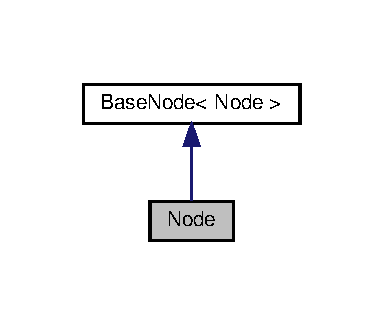
\includegraphics[width=184pt]{class_node__inherit__graph}
\end{center}
\end{figure}


Collaboration diagram for Node\+:
\nopagebreak
\begin{figure}[H]
\begin{center}
\leavevmode
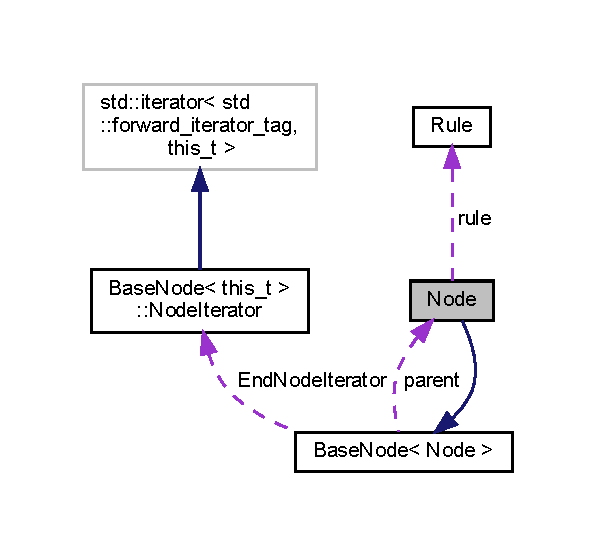
\includegraphics[width=286pt]{class_node__coll__graph}
\end{center}
\end{figure}
\doxysubsection*{Public Member Functions}
\begin{DoxyCompactItemize}
\item 
\mbox{\hyperlink{class_node_ae33050869651f64551da2d13ad2a9dbc}{Node}} (const \mbox{\hyperlink{class_rule}{Rule}} $\ast$r=nullptr, double \+\_\+lp=0.\+0, bool cr=true)
\item 
\mbox{\hyperlink{class_node_a277918b68827f6ffd8150f450b0c12c3}{Node}} (const \mbox{\hyperlink{class_node}{Node}} \&n)
\item 
\mbox{\hyperlink{class_node_a87c9938dcd77c169802a732c98204945}{Node}} (\mbox{\hyperlink{class_node}{Node}} \&\&n)
\item 
virtual \mbox{\hyperlink{class_node_af5e3fa79300bf5f3f2f3ecae6e795a94}{$\sim$\+Node}} ()
\item 
\mbox{\hyperlink{_nonterminal_8h_a1c5bfe9b903f69c83bbde5da7035fef3}{nonterminal\+\_\+t}} \mbox{\hyperlink{class_node_aa727c354e38f60fb1560d72ae1aaa9af}{type}} (const size\+\_\+t i) const
\item 
void \mbox{\hyperlink{class_node_afff50c3712b8e30fffd479cad4eee023}{set\+\_\+child}} (size\+\_\+t i, \mbox{\hyperlink{class_node}{Node}} \&n)
\item 
void \mbox{\hyperlink{class_node_a486882370d2c9592c6eabb52a3289253}{set\+\_\+child}} (size\+\_\+t i, \mbox{\hyperlink{class_node}{Node}} \&\&n)
\item 
void \mbox{\hyperlink{class_node_addbfe90949f473c91203389f48095cf0}{operator=}} (const \mbox{\hyperlink{class_node}{Node}} \&n)
\item 
void \mbox{\hyperlink{class_node_abcd5c8ca2ea54716a72f7e27f9a9c937}{operator=}} (\mbox{\hyperlink{class_node}{Node}} \&\&n)
\item 
bool \mbox{\hyperlink{class_node_a8b05feb361beb04d465619751a2297b1}{operator$<$}} (const \mbox{\hyperlink{class_node}{Node}} \&n) const
\item 
\mbox{\hyperlink{_nonterminal_8h_a1c5bfe9b903f69c83bbde5da7035fef3}{nonterminal\+\_\+t}} \mbox{\hyperlink{class_node_a4abe3acdc804489a01ef13a25b130fd8}{nt}} () const
\item 
bool \mbox{\hyperlink{class_node_a895ef3b66f975fbaec1e5866a57afbed}{is\+\_\+null}} () const
\item 
virtual size\+\_\+t \mbox{\hyperlink{class_node_a9dde16ce87ed78ca8c49f8b4c3be42f3}{count\+\_\+nonnull}} () const
\item 
{\footnotesize template$<$typename T $>$ }\\T \mbox{\hyperlink{class_node_ac91282056a0df2835f1579bdd21c93e1}{sum}} (std\+::function$<$ T(const \mbox{\hyperlink{class_node}{Node}} \&)$>$ \&f) const
\item 
{\footnotesize template$<$typename T $>$ }\\T \mbox{\hyperlink{class_node_a089e99addd93f91b2ef5a9d0c3e6bdeb}{sum}} (T($\ast$f)(const \mbox{\hyperlink{class_node}{Node}} \&)) const
\item 
bool \mbox{\hyperlink{class_node_ac6f1a0f5274eae688c1959aecbfde2b0}{all}} (std\+::function$<$ bool(const \mbox{\hyperlink{class_node}{Node}} \&)$>$ \&f) const
\item 
void \mbox{\hyperlink{class_node_adefac3cb7b411321c5af15dad1484834}{map}} (const std\+::function$<$ void(\mbox{\hyperlink{class_node}{Node}} \&)$>$ \&f)
\item 
virtual bool \mbox{\hyperlink{class_node_ac2e36754ba8b1b1d452deeb2bdbd346f}{is\+\_\+complete}} () const
\item 
virtual std\+::string \mbox{\hyperlink{class_node_a5d2a0e17dd2a00a79e6d1f763c9114d0}{string}} (bool usedot=true) const override
\item 
virtual std\+::string \mbox{\hyperlink{class_node_a70e879ceb71f47787137572d9bee8efa}{parseable}} () const
\item 
{\footnotesize template$<$typename Grammar\+\_\+t $>$ }\\int \mbox{\hyperlink{class_node_a2300ca04a56aeca14977915c4de0f53e}{linearize}} (Program \&program) const
\item 
virtual bool \mbox{\hyperlink{class_node_a8f42de356c047dd52472d24ace4d42c5}{operator==}} (const \mbox{\hyperlink{class_node}{Node}} \&n) const override
\item 
virtual size\+\_\+t \mbox{\hyperlink{class_node_a212f2e1ba4ff71de6954b0b791d89979}{hash}} (size\+\_\+t \mbox{\hyperlink{class_base_node_a4bab446840126b79f4d70cdc9bc6974c}{depth}}=0) const
\end{DoxyCompactItemize}
\doxysubsection*{Public Attributes}
\begin{DoxyCompactItemize}
\item 
const \mbox{\hyperlink{class_rule}{Rule}} $\ast$ \mbox{\hyperlink{class_node_a02f5c9463cceb270ad5730760f19c722}{rule}}
\item 
double \mbox{\hyperlink{class_node_a298eaa3743b774a3f9ef396e1dc42a08}{lp}}
\item 
bool \mbox{\hyperlink{class_node_a98c14a51b240fbc7e438f40a12276257}{can\+\_\+resample}}
\end{DoxyCompactItemize}
\doxysubsection*{Static Public Attributes}
\begin{DoxyCompactItemize}
\item 
const static char \mbox{\hyperlink{class_node_a72d47382356d51bdff43636f2c20c140}{N\+T\+Delimiter}} = \textquotesingle{}\+:\textquotesingle{}
\item 
const static char \mbox{\hyperlink{class_node_aa053fff4aee5ed47843a86d661632f15}{Rule\+Delimiter}} = \textquotesingle{};\textquotesingle{}
\end{DoxyCompactItemize}
\doxysubsection*{Friends}
\begin{DoxyCompactItemize}
\item 
class \mbox{\hyperlink{class_node_ae875dded1044564c83cdc7147d86dfbf}{Base\+Node$<$ Node $>$}}
\end{DoxyCompactItemize}
\doxysubsection*{Additional Inherited Members}


\doxysubsection{Constructor \& Destructor Documentation}
\mbox{\Hypertarget{class_node_ae33050869651f64551da2d13ad2a9dbc}\label{class_node_ae33050869651f64551da2d13ad2a9dbc}} 
\index{Node@{Node}!Node@{Node}}
\index{Node@{Node}!Node@{Node}}
\doxysubsubsection{\texorpdfstring{Node()}{Node()}\hspace{0.1cm}{\footnotesize\ttfamily [1/3]}}
{\footnotesize\ttfamily Node\+::\+Node (\begin{DoxyParamCaption}\item[{const \mbox{\hyperlink{class_rule}{Rule}} $\ast$}]{r = {\ttfamily nullptr},  }\item[{double}]{\+\_\+lp = {\ttfamily 0.0},  }\item[{bool}]{cr = {\ttfamily true} }\end{DoxyParamCaption})\hspace{0.3cm}{\ttfamily [inline]}}

\mbox{\Hypertarget{class_node_a277918b68827f6ffd8150f450b0c12c3}\label{class_node_a277918b68827f6ffd8150f450b0c12c3}} 
\index{Node@{Node}!Node@{Node}}
\index{Node@{Node}!Node@{Node}}
\doxysubsubsection{\texorpdfstring{Node()}{Node()}\hspace{0.1cm}{\footnotesize\ttfamily [2/3]}}
{\footnotesize\ttfamily Node\+::\+Node (\begin{DoxyParamCaption}\item[{const \mbox{\hyperlink{class_node}{Node}} \&}]{n }\end{DoxyParamCaption})\hspace{0.3cm}{\ttfamily [inline]}}

\mbox{\Hypertarget{class_node_a87c9938dcd77c169802a732c98204945}\label{class_node_a87c9938dcd77c169802a732c98204945}} 
\index{Node@{Node}!Node@{Node}}
\index{Node@{Node}!Node@{Node}}
\doxysubsubsection{\texorpdfstring{Node()}{Node()}\hspace{0.1cm}{\footnotesize\ttfamily [3/3]}}
{\footnotesize\ttfamily Node\+::\+Node (\begin{DoxyParamCaption}\item[{\mbox{\hyperlink{class_node}{Node}} \&\&}]{n }\end{DoxyParamCaption})\hspace{0.3cm}{\ttfamily [inline]}}

\mbox{\Hypertarget{class_node_af5e3fa79300bf5f3f2f3ecae6e795a94}\label{class_node_af5e3fa79300bf5f3f2f3ecae6e795a94}} 
\index{Node@{Node}!````~Node@{$\sim$Node}}
\index{````~Node@{$\sim$Node}!Node@{Node}}
\doxysubsubsection{\texorpdfstring{$\sim$Node()}{~Node()}}
{\footnotesize\ttfamily virtual Node\+::$\sim$\+Node (\begin{DoxyParamCaption}{ }\end{DoxyParamCaption})\hspace{0.3cm}{\ttfamily [inline]}, {\ttfamily [virtual]}}



\doxysubsection{Member Function Documentation}
\mbox{\Hypertarget{class_node_ac6f1a0f5274eae688c1959aecbfde2b0}\label{class_node_ac6f1a0f5274eae688c1959aecbfde2b0}} 
\index{Node@{Node}!all@{all}}
\index{all@{all}!Node@{Node}}
\doxysubsubsection{\texorpdfstring{all()}{all()}}
{\footnotesize\ttfamily bool Node\+::all (\begin{DoxyParamCaption}\item[{std\+::function$<$ bool(const \mbox{\hyperlink{class_node}{Node}} \&)$>$ \&}]{f }\end{DoxyParamCaption}) const\hspace{0.3cm}{\ttfamily [inline]}}

Check if f is true of me and every node below 
\begin{DoxyParams}{Parameters}
{\em f} & \\
\hline
\end{DoxyParams}
\begin{DoxyReturn}{Returns}

\end{DoxyReturn}
\mbox{\Hypertarget{class_node_a9dde16ce87ed78ca8c49f8b4c3be42f3}\label{class_node_a9dde16ce87ed78ca8c49f8b4c3be42f3}} 
\index{Node@{Node}!count\_nonnull@{count\_nonnull}}
\index{count\_nonnull@{count\_nonnull}!Node@{Node}}
\doxysubsubsection{\texorpdfstring{count\_nonnull()}{count\_nonnull()}}
{\footnotesize\ttfamily virtual size\+\_\+t Node\+::count\+\_\+nonnull (\begin{DoxyParamCaption}{ }\end{DoxyParamCaption}) const\hspace{0.3cm}{\ttfamily [inline]}, {\ttfamily [virtual]}}

How many nodes total are below me? 
\begin{DoxyParams}{Parameters}
{\em n} & \\
\hline
\end{DoxyParams}
\begin{DoxyReturn}{Returns}

\end{DoxyReturn}
\mbox{\Hypertarget{class_node_a212f2e1ba4ff71de6954b0b791d89979}\label{class_node_a212f2e1ba4ff71de6954b0b791d89979}} 
\index{Node@{Node}!hash@{hash}}
\index{hash@{hash}!Node@{Node}}
\doxysubsubsection{\texorpdfstring{hash()}{hash()}}
{\footnotesize\ttfamily virtual size\+\_\+t Node\+::hash (\begin{DoxyParamCaption}\item[{size\+\_\+t}]{depth = {\ttfamily 0} }\end{DoxyParamCaption}) const\hspace{0.3cm}{\ttfamily [inline]}, {\ttfamily [virtual]}}

Hash a tree by hashing the rule and everything below. 
\begin{DoxyParams}{Parameters}
{\em depth} & \\
\hline
\end{DoxyParams}
\begin{DoxyReturn}{Returns}

\end{DoxyReturn}
\mbox{\Hypertarget{class_node_ac2e36754ba8b1b1d452deeb2bdbd346f}\label{class_node_ac2e36754ba8b1b1d452deeb2bdbd346f}} 
\index{Node@{Node}!is\_complete@{is\_complete}}
\index{is\_complete@{is\_complete}!Node@{Node}}
\doxysubsubsection{\texorpdfstring{is\_complete()}{is\_complete()}}
{\footnotesize\ttfamily virtual bool Node\+::is\+\_\+complete (\begin{DoxyParamCaption}{ }\end{DoxyParamCaption}) const\hspace{0.3cm}{\ttfamily [inline]}, {\ttfamily [virtual]}}

A tree is complete if it contains no null nodes below it. \begin{DoxyReturn}{Returns}

\end{DoxyReturn}
\mbox{\Hypertarget{class_node_a895ef3b66f975fbaec1e5866a57afbed}\label{class_node_a895ef3b66f975fbaec1e5866a57afbed}} 
\index{Node@{Node}!is\_null@{is\_null}}
\index{is\_null@{is\_null}!Node@{Node}}
\doxysubsubsection{\texorpdfstring{is\_null()}{is\_null()}}
{\footnotesize\ttfamily bool Node\+::is\+\_\+null (\begin{DoxyParamCaption}{ }\end{DoxyParamCaption}) const\hspace{0.3cm}{\ttfamily [inline]}}

Am I a null node? \begin{DoxyReturn}{Returns}

\end{DoxyReturn}
\mbox{\Hypertarget{class_node_a2300ca04a56aeca14977915c4de0f53e}\label{class_node_a2300ca04a56aeca14977915c4de0f53e}} 
\index{Node@{Node}!linearize@{linearize}}
\index{linearize@{linearize}!Node@{Node}}
\doxysubsubsection{\texorpdfstring{linearize()}{linearize()}}
{\footnotesize\ttfamily template$<$typename Grammar\+\_\+t $>$ \\
int Node\+::linearize (\begin{DoxyParamCaption}\item[{Program \&}]{program }\end{DoxyParamCaption}) const\hspace{0.3cm}{\ttfamily [inline]}}

convert tree to a linear sequence of operations. To do this, we first linearize the kids, leaving their values as the top on the stack then we compute our value, remove our kids\textquotesingle{} values to clean up the stack, and push on our return the only fanciness is for if\+: here we will use the following layout $<$\+T\+O\+P O\+F S\+T\+A\+C\+K$>$ $<$bool$>$ op\+\_\+\+I\+F(xsize) X-\/branch J\+U\+M\+P(ysize) Y-\/branch

N\+O\+TE\+: Inline here lets gcc inline a few recursions of this function, which ends up speeding us up a bit (otherwise recursive inlining only happens at -\/O3) This optimization is why we do set max-\/inline-\/insns-\/recursive in Fleet.\+mk 
\begin{DoxyParams}{Parameters}
{\em ops} & \\
\hline
\end{DoxyParams}
\begin{DoxyReturn}{Returns}
This returns the {\itshape size} of the program that was pushed onto ops. This is useful for saving us lots of calls to program\+\_\+size, which ends up being an important optimization.
\end{DoxyReturn}
\mbox{\Hypertarget{class_node_adefac3cb7b411321c5af15dad1484834}\label{class_node_adefac3cb7b411321c5af15dad1484834}} 
\index{Node@{Node}!map@{map}}
\index{map@{map}!Node@{Node}}
\doxysubsubsection{\texorpdfstring{map()}{map()}}
{\footnotesize\ttfamily void Node\+::map (\begin{DoxyParamCaption}\item[{const std\+::function$<$ void(\mbox{\hyperlink{class_node}{Node}} \&)$>$ \&}]{f }\end{DoxyParamCaption})\hspace{0.3cm}{\ttfamily [inline]}}

Apply f to me and everything below. ~\newline
 
\begin{DoxyParams}{Parameters}
{\em f} & \\
\hline
\end{DoxyParams}
\mbox{\Hypertarget{class_node_a4abe3acdc804489a01ef13a25b130fd8}\label{class_node_a4abe3acdc804489a01ef13a25b130fd8}} 
\index{Node@{Node}!nt@{nt}}
\index{nt@{nt}!Node@{Node}}
\doxysubsubsection{\texorpdfstring{nt()}{nt()}}
{\footnotesize\ttfamily \mbox{\hyperlink{_nonterminal_8h_a1c5bfe9b903f69c83bbde5da7035fef3}{nonterminal\+\_\+t}} Node\+::nt (\begin{DoxyParamCaption}{ }\end{DoxyParamCaption}) const\hspace{0.3cm}{\ttfamily [inline]}}

What nonterminal type do I return? \begin{DoxyReturn}{Returns}

\end{DoxyReturn}
\mbox{\Hypertarget{class_node_a8b05feb361beb04d465619751a2297b1}\label{class_node_a8b05feb361beb04d465619751a2297b1}} 
\index{Node@{Node}!operator$<$@{operator$<$}}
\index{operator$<$@{operator$<$}!Node@{Node}}
\doxysubsubsection{\texorpdfstring{operator$<$()}{operator<()}}
{\footnotesize\ttfamily bool Node\+::operator$<$ (\begin{DoxyParamCaption}\item[{const \mbox{\hyperlink{class_node}{Node}} \&}]{n }\end{DoxyParamCaption}) const\hspace{0.3cm}{\ttfamily [inline]}}

\mbox{\Hypertarget{class_node_addbfe90949f473c91203389f48095cf0}\label{class_node_addbfe90949f473c91203389f48095cf0}} 
\index{Node@{Node}!operator=@{operator=}}
\index{operator=@{operator=}!Node@{Node}}
\doxysubsubsection{\texorpdfstring{operator=()}{operator=()}\hspace{0.1cm}{\footnotesize\ttfamily [1/2]}}
{\footnotesize\ttfamily void Node\+::operator= (\begin{DoxyParamCaption}\item[{const \mbox{\hyperlink{class_node}{Node}} \&}]{n }\end{DoxyParamCaption})\hspace{0.3cm}{\ttfamily [inline]}}

\mbox{\Hypertarget{class_node_abcd5c8ca2ea54716a72f7e27f9a9c937}\label{class_node_abcd5c8ca2ea54716a72f7e27f9a9c937}} 
\index{Node@{Node}!operator=@{operator=}}
\index{operator=@{operator=}!Node@{Node}}
\doxysubsubsection{\texorpdfstring{operator=()}{operator=()}\hspace{0.1cm}{\footnotesize\ttfamily [2/2]}}
{\footnotesize\ttfamily void Node\+::operator= (\begin{DoxyParamCaption}\item[{\mbox{\hyperlink{class_node}{Node}} \&\&}]{n }\end{DoxyParamCaption})\hspace{0.3cm}{\ttfamily [inline]}}

\mbox{\Hypertarget{class_node_a8f42de356c047dd52472d24ace4d42c5}\label{class_node_a8f42de356c047dd52472d24ace4d42c5}} 
\index{Node@{Node}!operator==@{operator==}}
\index{operator==@{operator==}!Node@{Node}}
\doxysubsubsection{\texorpdfstring{operator==()}{operator==()}}
{\footnotesize\ttfamily virtual bool Node\+::operator== (\begin{DoxyParamCaption}\item[{const \mbox{\hyperlink{class_node}{Node}} \&}]{n }\end{DoxyParamCaption}) const\hspace{0.3cm}{\ttfamily [inline]}, {\ttfamily [override]}, {\ttfamily [virtual]}}

Check equality between notes. Note this compares rule objects. 
\begin{DoxyParams}{Parameters}
{\em n} & \\
\hline
\end{DoxyParams}
\begin{DoxyReturn}{Returns}

\end{DoxyReturn}


Reimplemented from \mbox{\hyperlink{class_base_node_a33bb5c59122f6b2778d39a0eaa0151d7}{Base\+Node$<$ Node $>$}}.

\mbox{\Hypertarget{class_node_a70e879ceb71f47787137572d9bee8efa}\label{class_node_a70e879ceb71f47787137572d9bee8efa}} 
\index{Node@{Node}!parseable@{parseable}}
\index{parseable@{parseable}!Node@{Node}}
\doxysubsubsection{\texorpdfstring{parseable()}{parseable()}}
{\footnotesize\ttfamily virtual std\+::string Node\+::parseable (\begin{DoxyParamCaption}{ }\end{DoxyParamCaption}) const\hspace{0.3cm}{\ttfamily [inline]}, {\ttfamily [virtual]}}

Create a string that can be parsed according to \mbox{\hyperlink{class_grammar_a63a4c7f6584fdd70aaa2882a19c2f04f}{Grammar.\+from\+\_\+parseable}} \begin{DoxyReturn}{Returns}

\end{DoxyReturn}
\mbox{\Hypertarget{class_node_a486882370d2c9592c6eabb52a3289253}\label{class_node_a486882370d2c9592c6eabb52a3289253}} 
\index{Node@{Node}!set\_child@{set\_child}}
\index{set\_child@{set\_child}!Node@{Node}}
\doxysubsubsection{\texorpdfstring{set\_child()}{set\_child()}\hspace{0.1cm}{\footnotesize\ttfamily [1/2]}}
{\footnotesize\ttfamily void Node\+::set\+\_\+child (\begin{DoxyParamCaption}\item[{size\+\_\+t}]{i,  }\item[{\mbox{\hyperlink{class_node}{Node}} \&\&}]{n }\end{DoxyParamCaption})\hspace{0.3cm}{\ttfamily [inline]}}

Set my child to n. N\+O\+TE\+: This one needs to be used, rather than accessing children directly, because we have to set parent pointers and indices. 
\begin{DoxyParams}{Parameters}
{\em i} & \\
\hline
{\em n} & \\
\hline
\end{DoxyParams}
\mbox{\Hypertarget{class_node_afff50c3712b8e30fffd479cad4eee023}\label{class_node_afff50c3712b8e30fffd479cad4eee023}} 
\index{Node@{Node}!set\_child@{set\_child}}
\index{set\_child@{set\_child}!Node@{Node}}
\doxysubsubsection{\texorpdfstring{set\_child()}{set\_child()}\hspace{0.1cm}{\footnotesize\ttfamily [2/2]}}
{\footnotesize\ttfamily void Node\+::set\+\_\+child (\begin{DoxyParamCaption}\item[{size\+\_\+t}]{i,  }\item[{\mbox{\hyperlink{class_node}{Node}} \&}]{n }\end{DoxyParamCaption})\hspace{0.3cm}{\ttfamily [inline]}}

Set my child to n. N\+O\+TE\+: This one needs to be used, rather than accessing children directly, because we have to set parent pointers and indices. 
\begin{DoxyParams}{Parameters}
{\em i} & \\
\hline
{\em n} & \\
\hline
\end{DoxyParams}
\mbox{\Hypertarget{class_node_a5d2a0e17dd2a00a79e6d1f763c9114d0}\label{class_node_a5d2a0e17dd2a00a79e6d1f763c9114d0}} 
\index{Node@{Node}!string@{string}}
\index{string@{string}!Node@{Node}}
\doxysubsubsection{\texorpdfstring{string()}{string()}}
{\footnotesize\ttfamily virtual std\+::string Node\+::string (\begin{DoxyParamCaption}\item[{bool}]{usedot = {\ttfamily true} }\end{DoxyParamCaption}) const\hspace{0.3cm}{\ttfamily [inline]}, {\ttfamily [override]}, {\ttfamily [virtual]}}

Convert a tree to a string, using each node\textquotesingle{}s format. ~\newline
 
\begin{DoxyParams}{Parameters}
{\em usedot} & -\/ do we print a dot in front of pieces of nodes that cannot be resampled? Useful for mcts \\
\hline
\end{DoxyParams}
\begin{DoxyReturn}{Returns}

\end{DoxyReturn}


Reimplemented from \mbox{\hyperlink{class_base_node_a079dae7bec84f4de8eef6d6cb9368a22}{Base\+Node$<$ Node $>$}}.

\mbox{\Hypertarget{class_node_ac91282056a0df2835f1579bdd21c93e1}\label{class_node_ac91282056a0df2835f1579bdd21c93e1}} 
\index{Node@{Node}!sum@{sum}}
\index{sum@{sum}!Node@{Node}}
\doxysubsubsection{\texorpdfstring{sum()}{sum()}\hspace{0.1cm}{\footnotesize\ttfamily [1/2]}}
{\footnotesize\ttfamily template$<$typename T $>$ \\
T Node\+::sum (\begin{DoxyParamCaption}\item[{std\+::function$<$ T(const \mbox{\hyperlink{class_node}{Node}} \&)$>$ \&}]{f }\end{DoxyParamCaption}) const\hspace{0.3cm}{\ttfamily [inline]}}

Apply f to me and everything below me, adding up the result. 
\begin{DoxyParams}{Parameters}
{\em f} & \\
\hline
\end{DoxyParams}
\begin{DoxyReturn}{Returns}

\end{DoxyReturn}
\mbox{\Hypertarget{class_node_a089e99addd93f91b2ef5a9d0c3e6bdeb}\label{class_node_a089e99addd93f91b2ef5a9d0c3e6bdeb}} 
\index{Node@{Node}!sum@{sum}}
\index{sum@{sum}!Node@{Node}}
\doxysubsubsection{\texorpdfstring{sum()}{sum()}\hspace{0.1cm}{\footnotesize\ttfamily [2/2]}}
{\footnotesize\ttfamily template$<$typename T $>$ \\
T Node\+::sum (\begin{DoxyParamCaption}\item[{T($\ast$)(const \mbox{\hyperlink{class_node}{Node}} \&)}]{f }\end{DoxyParamCaption}) const\hspace{0.3cm}{\ttfamily [inline]}}

\mbox{\Hypertarget{class_node_aa727c354e38f60fb1560d72ae1aaa9af}\label{class_node_aa727c354e38f60fb1560d72ae1aaa9af}} 
\index{Node@{Node}!type@{type}}
\index{type@{type}!Node@{Node}}
\doxysubsubsection{\texorpdfstring{type()}{type()}}
{\footnotesize\ttfamily \mbox{\hyperlink{_nonterminal_8h_a1c5bfe9b903f69c83bbde5da7035fef3}{nonterminal\+\_\+t}} Node\+::type (\begin{DoxyParamCaption}\item[{const size\+\_\+t}]{i }\end{DoxyParamCaption}) const\hspace{0.3cm}{\ttfamily [inline]}}

Return the type of the i\textquotesingle{}th child 
\begin{DoxyParams}{Parameters}
{\em i} & \\
\hline
\end{DoxyParams}
\begin{DoxyReturn}{Returns}

\end{DoxyReturn}


\doxysubsection{Friends And Related Function Documentation}
\mbox{\Hypertarget{class_node_ae875dded1044564c83cdc7147d86dfbf}\label{class_node_ae875dded1044564c83cdc7147d86dfbf}} 
\index{Node@{Node}!BaseNode$<$ Node $>$@{BaseNode$<$ Node $>$}}
\index{BaseNode$<$ Node $>$@{BaseNode$<$ Node $>$}!Node@{Node}}
\doxysubsubsection{\texorpdfstring{BaseNode$<$ Node $>$}{BaseNode< Node >}}
{\footnotesize\ttfamily friend class \mbox{\hyperlink{class_base_node}{Base\+Node}}$<$ \mbox{\hyperlink{class_node}{Node}} $>$\hspace{0.3cm}{\ttfamily [friend]}}



\doxysubsection{Member Data Documentation}
\mbox{\Hypertarget{class_node_a98c14a51b240fbc7e438f40a12276257}\label{class_node_a98c14a51b240fbc7e438f40a12276257}} 
\index{Node@{Node}!can\_resample@{can\_resample}}
\index{can\_resample@{can\_resample}!Node@{Node}}
\doxysubsubsection{\texorpdfstring{can\_resample}{can\_resample}}
{\footnotesize\ttfamily bool Node\+::can\+\_\+resample}

\mbox{\Hypertarget{class_node_a298eaa3743b774a3f9ef396e1dc42a08}\label{class_node_a298eaa3743b774a3f9ef396e1dc42a08}} 
\index{Node@{Node}!lp@{lp}}
\index{lp@{lp}!Node@{Node}}
\doxysubsubsection{\texorpdfstring{lp}{lp}}
{\footnotesize\ttfamily double Node\+::lp}

\mbox{\Hypertarget{class_node_a72d47382356d51bdff43636f2c20c140}\label{class_node_a72d47382356d51bdff43636f2c20c140}} 
\index{Node@{Node}!NTDelimiter@{NTDelimiter}}
\index{NTDelimiter@{NTDelimiter}!Node@{Node}}
\doxysubsubsection{\texorpdfstring{NTDelimiter}{NTDelimiter}}
{\footnotesize\ttfamily const static char Node\+::\+N\+T\+Delimiter = \textquotesingle{}\+:\textquotesingle{}\hspace{0.3cm}{\ttfamily [static]}}

\mbox{\Hypertarget{class_node_a02f5c9463cceb270ad5730760f19c722}\label{class_node_a02f5c9463cceb270ad5730760f19c722}} 
\index{Node@{Node}!rule@{rule}}
\index{rule@{rule}!Node@{Node}}
\doxysubsubsection{\texorpdfstring{rule}{rule}}
{\footnotesize\ttfamily const \mbox{\hyperlink{class_rule}{Rule}}$\ast$ Node\+::rule}

\mbox{\Hypertarget{class_node_aa053fff4aee5ed47843a86d661632f15}\label{class_node_aa053fff4aee5ed47843a86d661632f15}} 
\index{Node@{Node}!RuleDelimiter@{RuleDelimiter}}
\index{RuleDelimiter@{RuleDelimiter}!Node@{Node}}
\doxysubsubsection{\texorpdfstring{RuleDelimiter}{RuleDelimiter}}
{\footnotesize\ttfamily const static char Node\+::\+Rule\+Delimiter = \textquotesingle{};\textquotesingle{}\hspace{0.3cm}{\ttfamily [static]}}



The documentation for this class was generated from the following file\+:\begin{DoxyCompactItemize}
\item 
src/\+Grammar/\mbox{\hyperlink{_node_8h}{Node.\+h}}\end{DoxyCompactItemize}

\hypertarget{class_base_node_1_1_node_iterator}{}\doxysection{Base\+Node$<$ this\+\_\+t $>$\+::Node\+Iterator Class Reference}
\label{class_base_node_1_1_node_iterator}\index{BaseNode$<$ this\_t $>$::NodeIterator@{BaseNode$<$ this\_t $>$::NodeIterator}}


{\ttfamily \#include $<$Base\+Node.\+h$>$}



Inheritance diagram for Base\+Node$<$ this\+\_\+t $>$\+::Node\+Iterator\+:\nopagebreak
\begin{figure}[H]
\begin{center}
\leavevmode
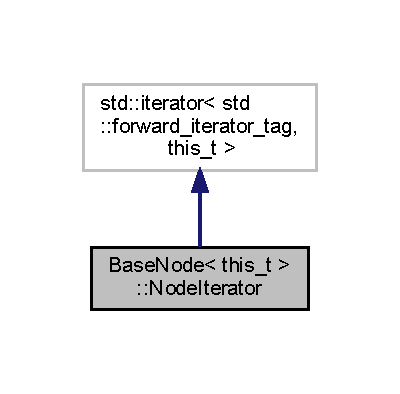
\includegraphics[width=192pt]{class_base_node_1_1_node_iterator__inherit__graph}
\end{center}
\end{figure}


Collaboration diagram for Base\+Node$<$ this\+\_\+t $>$\+::Node\+Iterator\+:\nopagebreak
\begin{figure}[H]
\begin{center}
\leavevmode
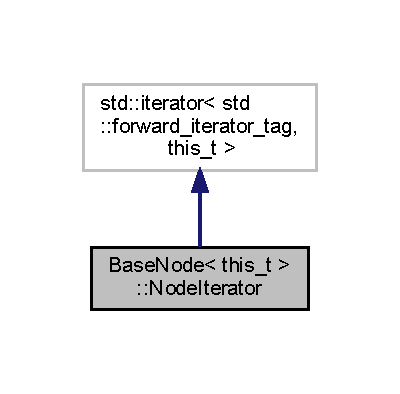
\includegraphics[width=192pt]{class_base_node_1_1_node_iterator__coll__graph}
\end{center}
\end{figure}
\doxysubsection*{Public Member Functions}
\begin{DoxyCompactItemize}
\item 
\mbox{\hyperlink{class_base_node_1_1_node_iterator_a9414dbb668b4b98f5377d434f8577dc6}{Node\+Iterator}} (const this\+\_\+t $\ast$n)
\item 
this\+\_\+t \& \mbox{\hyperlink{class_base_node_1_1_node_iterator_ae8543e096a3169c59238cb4a2d872d88}{operator$\ast$}} () const
\item 
this\+\_\+t $\ast$ \mbox{\hyperlink{class_base_node_1_1_node_iterator_a6d9525f787b4339909c6236b93905ec2}{operator-\/$>$}} () const
\item 
\mbox{\hyperlink{class_base_node_1_1_node_iterator}{Node\+Iterator}} \& \mbox{\hyperlink{class_base_node_1_1_node_iterator_a951d2910a7c8246bf882cd684ac12f64}{operator++}} (int blah)
\item 
\mbox{\hyperlink{class_base_node_1_1_node_iterator}{Node\+Iterator}} \& \mbox{\hyperlink{class_base_node_1_1_node_iterator_a5fd7a29fd07fdc3e60302bdc8a6cb61f}{operator++}} ()
\item 
\mbox{\hyperlink{class_base_node_1_1_node_iterator}{Node\+Iterator}} \& \mbox{\hyperlink{class_base_node_1_1_node_iterator_a347656df237dcc3de8ad40896b260cf8}{operator+}} (size\+\_\+t n)
\item 
bool \mbox{\hyperlink{class_base_node_1_1_node_iterator_af3e1ab104af103b5536e4b9237fba588}{operator==}} (const \mbox{\hyperlink{class_base_node_1_1_node_iterator}{Node\+Iterator}} \&rhs)
\item 
bool \mbox{\hyperlink{class_base_node_1_1_node_iterator_a10e2c9cd9a879e6a5779981badfa335b}{operator!=}} (const \mbox{\hyperlink{class_base_node_1_1_node_iterator}{Node\+Iterator}} \&rhs)
\end{DoxyCompactItemize}
\doxysubsection*{Protected Attributes}
\begin{DoxyCompactItemize}
\item 
this\+\_\+t $\ast$ \mbox{\hyperlink{class_base_node_1_1_node_iterator_a64b6d98532282b0d5c4b00454f2dd9cb}{current}}
\item 
const this\+\_\+t $\ast$ \mbox{\hyperlink{class_base_node_1_1_node_iterator_a0583943df31aaf646c09338a1ba866c1}{start}}
\end{DoxyCompactItemize}


\doxysubsection{Detailed Description}
\subsubsection*{template$<$typename this\+\_\+t$>$\newline
class Base\+Node$<$ this\+\_\+t $>$\+::\+Node\+Iterator}

\begin{DoxyAuthor}{Author}
piantado 
\end{DoxyAuthor}
\begin{DoxyDate}{Date}
03/07/20 
\end{DoxyDate}


\doxysubsection{Constructor \& Destructor Documentation}
\mbox{\Hypertarget{class_base_node_1_1_node_iterator_a9414dbb668b4b98f5377d434f8577dc6}\label{class_base_node_1_1_node_iterator_a9414dbb668b4b98f5377d434f8577dc6}} 
\index{BaseNode$<$ this\_t $>$::NodeIterator@{BaseNode$<$ this\_t $>$::NodeIterator}!NodeIterator@{NodeIterator}}
\index{NodeIterator@{NodeIterator}!BaseNode$<$ this\_t $>$::NodeIterator@{BaseNode$<$ this\_t $>$::NodeIterator}}
\doxysubsubsection{\texorpdfstring{NodeIterator()}{NodeIterator()}}
{\footnotesize\ttfamily template$<$typename this\+\_\+t $>$ \\
\mbox{\hyperlink{class_base_node}{Base\+Node}}$<$ this\+\_\+t $>$\+::Node\+Iterator\+::\+Node\+Iterator (\begin{DoxyParamCaption}\item[{const this\+\_\+t $\ast$}]{n }\end{DoxyParamCaption})\hspace{0.3cm}{\ttfamily [inline]}}



\doxysubsection{Member Function Documentation}
\mbox{\Hypertarget{class_base_node_1_1_node_iterator_a10e2c9cd9a879e6a5779981badfa335b}\label{class_base_node_1_1_node_iterator_a10e2c9cd9a879e6a5779981badfa335b}} 
\index{BaseNode$<$ this\_t $>$::NodeIterator@{BaseNode$<$ this\_t $>$::NodeIterator}!operator"!=@{operator"!=}}
\index{operator"!=@{operator"!=}!BaseNode$<$ this\_t $>$::NodeIterator@{BaseNode$<$ this\_t $>$::NodeIterator}}
\doxysubsubsection{\texorpdfstring{operator"!=()}{operator!=()}}
{\footnotesize\ttfamily template$<$typename this\+\_\+t $>$ \\
bool \mbox{\hyperlink{class_base_node}{Base\+Node}}$<$ this\+\_\+t $>$\+::Node\+Iterator\+::operator!= (\begin{DoxyParamCaption}\item[{const \mbox{\hyperlink{class_base_node_1_1_node_iterator}{Node\+Iterator}} \&}]{rhs }\end{DoxyParamCaption})\hspace{0.3cm}{\ttfamily [inline]}}

\mbox{\Hypertarget{class_base_node_1_1_node_iterator_ae8543e096a3169c59238cb4a2d872d88}\label{class_base_node_1_1_node_iterator_ae8543e096a3169c59238cb4a2d872d88}} 
\index{BaseNode$<$ this\_t $>$::NodeIterator@{BaseNode$<$ this\_t $>$::NodeIterator}!operator$\ast$@{operator$\ast$}}
\index{operator$\ast$@{operator$\ast$}!BaseNode$<$ this\_t $>$::NodeIterator@{BaseNode$<$ this\_t $>$::NodeIterator}}
\doxysubsubsection{\texorpdfstring{operator$\ast$()}{operator*()}}
{\footnotesize\ttfamily template$<$typename this\+\_\+t $>$ \\
this\+\_\+t\& \mbox{\hyperlink{class_base_node}{Base\+Node}}$<$ this\+\_\+t $>$\+::Node\+Iterator\+::operator$\ast$ (\begin{DoxyParamCaption}{ }\end{DoxyParamCaption}) const\hspace{0.3cm}{\ttfamily [inline]}}

\mbox{\Hypertarget{class_base_node_1_1_node_iterator_a347656df237dcc3de8ad40896b260cf8}\label{class_base_node_1_1_node_iterator_a347656df237dcc3de8ad40896b260cf8}} 
\index{BaseNode$<$ this\_t $>$::NodeIterator@{BaseNode$<$ this\_t $>$::NodeIterator}!operator+@{operator+}}
\index{operator+@{operator+}!BaseNode$<$ this\_t $>$::NodeIterator@{BaseNode$<$ this\_t $>$::NodeIterator}}
\doxysubsubsection{\texorpdfstring{operator+()}{operator+()}}
{\footnotesize\ttfamily template$<$typename this\+\_\+t $>$ \\
\mbox{\hyperlink{class_base_node_1_1_node_iterator}{Node\+Iterator}}\& \mbox{\hyperlink{class_base_node}{Base\+Node}}$<$ this\+\_\+t $>$\+::Node\+Iterator\+::operator+ (\begin{DoxyParamCaption}\item[{size\+\_\+t}]{n }\end{DoxyParamCaption})\hspace{0.3cm}{\ttfamily [inline]}}

\mbox{\Hypertarget{class_base_node_1_1_node_iterator_a5fd7a29fd07fdc3e60302bdc8a6cb61f}\label{class_base_node_1_1_node_iterator_a5fd7a29fd07fdc3e60302bdc8a6cb61f}} 
\index{BaseNode$<$ this\_t $>$::NodeIterator@{BaseNode$<$ this\_t $>$::NodeIterator}!operator++@{operator++}}
\index{operator++@{operator++}!BaseNode$<$ this\_t $>$::NodeIterator@{BaseNode$<$ this\_t $>$::NodeIterator}}
\doxysubsubsection{\texorpdfstring{operator++()}{operator++()}\hspace{0.1cm}{\footnotesize\ttfamily [1/2]}}
{\footnotesize\ttfamily template$<$typename this\+\_\+t $>$ \\
\mbox{\hyperlink{class_base_node_1_1_node_iterator}{Node\+Iterator}}\& \mbox{\hyperlink{class_base_node}{Base\+Node}}$<$ this\+\_\+t $>$\+::Node\+Iterator\+::operator++ (\begin{DoxyParamCaption}{ }\end{DoxyParamCaption})\hspace{0.3cm}{\ttfamily [inline]}}

\mbox{\Hypertarget{class_base_node_1_1_node_iterator_a951d2910a7c8246bf882cd684ac12f64}\label{class_base_node_1_1_node_iterator_a951d2910a7c8246bf882cd684ac12f64}} 
\index{BaseNode$<$ this\_t $>$::NodeIterator@{BaseNode$<$ this\_t $>$::NodeIterator}!operator++@{operator++}}
\index{operator++@{operator++}!BaseNode$<$ this\_t $>$::NodeIterator@{BaseNode$<$ this\_t $>$::NodeIterator}}
\doxysubsubsection{\texorpdfstring{operator++()}{operator++()}\hspace{0.1cm}{\footnotesize\ttfamily [2/2]}}
{\footnotesize\ttfamily template$<$typename this\+\_\+t $>$ \\
\mbox{\hyperlink{class_base_node_1_1_node_iterator}{Node\+Iterator}}\& \mbox{\hyperlink{class_base_node}{Base\+Node}}$<$ this\+\_\+t $>$\+::Node\+Iterator\+::operator++ (\begin{DoxyParamCaption}\item[{int}]{blah }\end{DoxyParamCaption})\hspace{0.3cm}{\ttfamily [inline]}}

\mbox{\Hypertarget{class_base_node_1_1_node_iterator_a6d9525f787b4339909c6236b93905ec2}\label{class_base_node_1_1_node_iterator_a6d9525f787b4339909c6236b93905ec2}} 
\index{BaseNode$<$ this\_t $>$::NodeIterator@{BaseNode$<$ this\_t $>$::NodeIterator}!operator-\/$>$@{operator-\/$>$}}
\index{operator-\/$>$@{operator-\/$>$}!BaseNode$<$ this\_t $>$::NodeIterator@{BaseNode$<$ this\_t $>$::NodeIterator}}
\doxysubsubsection{\texorpdfstring{operator-\/$>$()}{operator->()}}
{\footnotesize\ttfamily template$<$typename this\+\_\+t $>$ \\
this\+\_\+t$\ast$ \mbox{\hyperlink{class_base_node}{Base\+Node}}$<$ this\+\_\+t $>$\+::Node\+Iterator\+::operator-\/$>$ (\begin{DoxyParamCaption}{ }\end{DoxyParamCaption}) const\hspace{0.3cm}{\ttfamily [inline]}}

\mbox{\Hypertarget{class_base_node_1_1_node_iterator_af3e1ab104af103b5536e4b9237fba588}\label{class_base_node_1_1_node_iterator_af3e1ab104af103b5536e4b9237fba588}} 
\index{BaseNode$<$ this\_t $>$::NodeIterator@{BaseNode$<$ this\_t $>$::NodeIterator}!operator==@{operator==}}
\index{operator==@{operator==}!BaseNode$<$ this\_t $>$::NodeIterator@{BaseNode$<$ this\_t $>$::NodeIterator}}
\doxysubsubsection{\texorpdfstring{operator==()}{operator==()}}
{\footnotesize\ttfamily template$<$typename this\+\_\+t $>$ \\
bool \mbox{\hyperlink{class_base_node}{Base\+Node}}$<$ this\+\_\+t $>$\+::Node\+Iterator\+::operator== (\begin{DoxyParamCaption}\item[{const \mbox{\hyperlink{class_base_node_1_1_node_iterator}{Node\+Iterator}} \&}]{rhs }\end{DoxyParamCaption})\hspace{0.3cm}{\ttfamily [inline]}}



\doxysubsection{Member Data Documentation}
\mbox{\Hypertarget{class_base_node_1_1_node_iterator_a64b6d98532282b0d5c4b00454f2dd9cb}\label{class_base_node_1_1_node_iterator_a64b6d98532282b0d5c4b00454f2dd9cb}} 
\index{BaseNode$<$ this\_t $>$::NodeIterator@{BaseNode$<$ this\_t $>$::NodeIterator}!current@{current}}
\index{current@{current}!BaseNode$<$ this\_t $>$::NodeIterator@{BaseNode$<$ this\_t $>$::NodeIterator}}
\doxysubsubsection{\texorpdfstring{current}{current}}
{\footnotesize\ttfamily template$<$typename this\+\_\+t $>$ \\
this\+\_\+t$\ast$ \mbox{\hyperlink{class_base_node}{Base\+Node}}$<$ this\+\_\+t $>$\+::Node\+Iterator\+::current\hspace{0.3cm}{\ttfamily [protected]}}

\mbox{\Hypertarget{class_base_node_1_1_node_iterator_a0583943df31aaf646c09338a1ba866c1}\label{class_base_node_1_1_node_iterator_a0583943df31aaf646c09338a1ba866c1}} 
\index{BaseNode$<$ this\_t $>$::NodeIterator@{BaseNode$<$ this\_t $>$::NodeIterator}!start@{start}}
\index{start@{start}!BaseNode$<$ this\_t $>$::NodeIterator@{BaseNode$<$ this\_t $>$::NodeIterator}}
\doxysubsubsection{\texorpdfstring{start}{start}}
{\footnotesize\ttfamily template$<$typename this\+\_\+t $>$ \\
const this\+\_\+t$\ast$ \mbox{\hyperlink{class_base_node}{Base\+Node}}$<$ this\+\_\+t $>$\+::Node\+Iterator\+::start\hspace{0.3cm}{\ttfamily [protected]}}



The documentation for this class was generated from the following file\+:\begin{DoxyCompactItemize}
\item 
src/\mbox{\hyperlink{_base_node_8h}{Base\+Node.\+h}}\end{DoxyCompactItemize}

\hypertarget{class_not_implemented_error}{}\doxysection{Not\+Implemented\+Error Class Reference}
\label{class_not_implemented_error}\index{NotImplementedError@{NotImplementedError}}


{\ttfamily \#include $<$Errors.\+h$>$}



Inheritance diagram for Not\+Implemented\+Error\+:\nopagebreak
\begin{figure}[H]
\begin{center}
\leavevmode
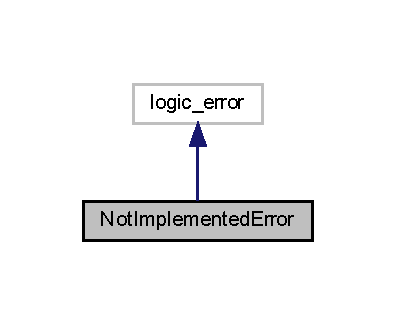
\includegraphics[width=190pt]{class_not_implemented_error__inherit__graph}
\end{center}
\end{figure}


Collaboration diagram for Not\+Implemented\+Error\+:\nopagebreak
\begin{figure}[H]
\begin{center}
\leavevmode
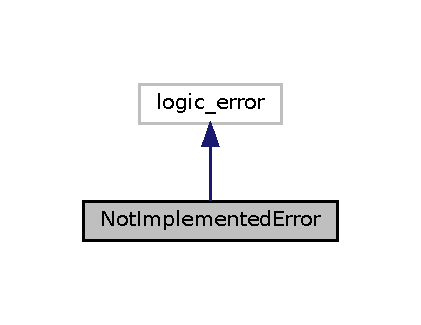
\includegraphics[width=190pt]{class_not_implemented_error__coll__graph}
\end{center}
\end{figure}
\doxysubsection*{Public Member Functions}
\begin{DoxyCompactItemize}
\item 
\mbox{\hyperlink{class_not_implemented_error_a715a224ab50633f41010e22d2033e6d8}{Not\+Implemented\+Error}} ()
\item 
\mbox{\hyperlink{class_not_implemented_error_a0fc1c5e8d9ea2da187ca3ddf0e65e8e9}{Not\+Implemented\+Error}} (std\+::string s)
\item 
virtual char const  $\ast$ \mbox{\hyperlink{class_not_implemented_error_a338a926dcaa356ac1b33cc0d7a093351}{what}} () const noexcept override
\end{DoxyCompactItemize}


\doxysubsection{Constructor \& Destructor Documentation}
\mbox{\Hypertarget{class_not_implemented_error_a715a224ab50633f41010e22d2033e6d8}\label{class_not_implemented_error_a715a224ab50633f41010e22d2033e6d8}} 
\index{NotImplementedError@{NotImplementedError}!NotImplementedError@{NotImplementedError}}
\index{NotImplementedError@{NotImplementedError}!NotImplementedError@{NotImplementedError}}
\doxysubsubsection{\texorpdfstring{NotImplementedError()}{NotImplementedError()}\hspace{0.1cm}{\footnotesize\ttfamily [1/2]}}
{\footnotesize\ttfamily Not\+Implemented\+Error\+::\+Not\+Implemented\+Error (\begin{DoxyParamCaption}{ }\end{DoxyParamCaption})\hspace{0.3cm}{\ttfamily [inline]}}

\mbox{\Hypertarget{class_not_implemented_error_a0fc1c5e8d9ea2da187ca3ddf0e65e8e9}\label{class_not_implemented_error_a0fc1c5e8d9ea2da187ca3ddf0e65e8e9}} 
\index{NotImplementedError@{NotImplementedError}!NotImplementedError@{NotImplementedError}}
\index{NotImplementedError@{NotImplementedError}!NotImplementedError@{NotImplementedError}}
\doxysubsubsection{\texorpdfstring{NotImplementedError()}{NotImplementedError()}\hspace{0.1cm}{\footnotesize\ttfamily [2/2]}}
{\footnotesize\ttfamily Not\+Implemented\+Error\+::\+Not\+Implemented\+Error (\begin{DoxyParamCaption}\item[{std\+::string}]{s }\end{DoxyParamCaption})\hspace{0.3cm}{\ttfamily [inline]}}



\doxysubsection{Member Function Documentation}
\mbox{\Hypertarget{class_not_implemented_error_a338a926dcaa356ac1b33cc0d7a093351}\label{class_not_implemented_error_a338a926dcaa356ac1b33cc0d7a093351}} 
\index{NotImplementedError@{NotImplementedError}!what@{what}}
\index{what@{what}!NotImplementedError@{NotImplementedError}}
\doxysubsubsection{\texorpdfstring{what()}{what()}}
{\footnotesize\ttfamily virtual char const$\ast$ Not\+Implemented\+Error\+::what (\begin{DoxyParamCaption}{ }\end{DoxyParamCaption}) const\hspace{0.3cm}{\ttfamily [inline]}, {\ttfamily [override]}, {\ttfamily [virtual]}, {\ttfamily [noexcept]}}



The documentation for this class was generated from the following file\+:\begin{DoxyCompactItemize}
\item 
src/\mbox{\hyperlink{_errors_8h}{Errors.\+h}}\end{DoxyCompactItemize}

\hypertarget{structnull__t}{}\doxysection{null\+\_\+t Struct Reference}
\label{structnull__t}\index{null\_t@{null\_t}}


{\ttfamily \#include $<$Miscellaneous.\+h$>$}



The documentation for this struct was generated from the following file\+:\begin{DoxyCompactItemize}
\item 
src/\mbox{\hyperlink{_miscellaneous_8h}{Miscellaneous.\+h}}\end{DoxyCompactItemize}

\hypertarget{class_parallel_inference_interface}{}\section{Parallel\+Inference\+Interface$<$ Args $>$ Class Template Reference}
\label{class_parallel_inference_interface}\index{Parallel\+Inference\+Interface$<$ Args $>$@{Parallel\+Inference\+Interface$<$ Args $>$}}


{\ttfamily \#include $<$Parallel\+Inference\+Interface.\+h$>$}

\subsection*{Public Member Functions}
\begin{DoxyCompactItemize}
\item 
virtual void \hyperlink{class_parallel_inference_interface_a79f626a400fbc11ed530c97f32dfd5c3}{run\+\_\+thread} (\hyperlink{struct_control}{Control} ctl, Args... args)=0
\item 
\hyperlink{class_parallel_inference_interface_a59989833c3d7fde08746087b29c7dcef}{Parallel\+Inference\+Interface} ()
\item 
unsigned long \hyperlink{class_parallel_inference_interface_aaa1fe948131956b21a89c8c267e46b6c}{next\+\_\+index} ()
\begin{DoxyCompactList}\small\item\em Return the next index to operate on (in a thread-\/safe way). \end{DoxyCompactList}\item 
void \hyperlink{class_parallel_inference_interface_a836204d148b8b5187d39e494d926d7b3}{run} (\hyperlink{struct_control}{Control} ctl, Args... args)
\begin{DoxyCompactList}\small\item\em Run is the main control interface. Copies of ctl get made and passed to each thread in run\+\_\+thread. \end{DoxyCompactList}\end{DoxyCompactItemize}
\subsection*{Public Attributes}
\begin{DoxyCompactItemize}
\item 
std\+::atomic$<$ size\+\_\+t $>$ \hyperlink{class_parallel_inference_interface_a1494ba5ab10b5fda9bca6acc39de37cb}{index}
\end{DoxyCompactItemize}


\subsection{Constructor \& Destructor Documentation}
\mbox{\Hypertarget{class_parallel_inference_interface_a59989833c3d7fde08746087b29c7dcef}\label{class_parallel_inference_interface_a59989833c3d7fde08746087b29c7dcef}} 
\index{Parallel\+Inference\+Interface@{Parallel\+Inference\+Interface}!Parallel\+Inference\+Interface@{Parallel\+Inference\+Interface}}
\index{Parallel\+Inference\+Interface@{Parallel\+Inference\+Interface}!Parallel\+Inference\+Interface@{Parallel\+Inference\+Interface}}
\subsubsection{\texorpdfstring{Parallel\+Inference\+Interface()}{ParallelInferenceInterface()}}
{\footnotesize\ttfamily template$<$typename... Args$>$ \\
\hyperlink{class_parallel_inference_interface}{Parallel\+Inference\+Interface}$<$ Args $>$\+::\hyperlink{class_parallel_inference_interface}{Parallel\+Inference\+Interface} (\begin{DoxyParamCaption}{ }\end{DoxyParamCaption})\hspace{0.3cm}{\ttfamily [inline]}}



\subsection{Member Function Documentation}
\mbox{\Hypertarget{class_parallel_inference_interface_aaa1fe948131956b21a89c8c267e46b6c}\label{class_parallel_inference_interface_aaa1fe948131956b21a89c8c267e46b6c}} 
\index{Parallel\+Inference\+Interface@{Parallel\+Inference\+Interface}!next\+\_\+index@{next\+\_\+index}}
\index{next\+\_\+index@{next\+\_\+index}!Parallel\+Inference\+Interface@{Parallel\+Inference\+Interface}}
\subsubsection{\texorpdfstring{next\+\_\+index()}{next\_index()}}
{\footnotesize\ttfamily template$<$typename... Args$>$ \\
unsigned long \hyperlink{class_parallel_inference_interface}{Parallel\+Inference\+Interface}$<$ Args $>$\+::next\+\_\+index (\begin{DoxyParamCaption}{ }\end{DoxyParamCaption})\hspace{0.3cm}{\ttfamily [inline]}}



Return the next index to operate on (in a thread-\/safe way). 

\begin{DoxyReturn}{Returns}

\end{DoxyReturn}
\mbox{\Hypertarget{class_parallel_inference_interface_a836204d148b8b5187d39e494d926d7b3}\label{class_parallel_inference_interface_a836204d148b8b5187d39e494d926d7b3}} 
\index{Parallel\+Inference\+Interface@{Parallel\+Inference\+Interface}!run@{run}}
\index{run@{run}!Parallel\+Inference\+Interface@{Parallel\+Inference\+Interface}}
\subsubsection{\texorpdfstring{run()}{run()}}
{\footnotesize\ttfamily template$<$typename... Args$>$ \\
void \hyperlink{class_parallel_inference_interface}{Parallel\+Inference\+Interface}$<$ Args $>$\+::run (\begin{DoxyParamCaption}\item[{\hyperlink{struct_control}{Control}}]{ctl,  }\item[{Args...}]{args }\end{DoxyParamCaption})\hspace{0.3cm}{\ttfamily [inline]}}



Run is the main control interface. Copies of ctl get made and passed to each thread in run\+\_\+thread. 


\begin{DoxyParams}{Parameters}
{\em ctl} & \\
\hline
\end{DoxyParams}
\mbox{\Hypertarget{class_parallel_inference_interface_a79f626a400fbc11ed530c97f32dfd5c3}\label{class_parallel_inference_interface_a79f626a400fbc11ed530c97f32dfd5c3}} 
\index{Parallel\+Inference\+Interface@{Parallel\+Inference\+Interface}!run\+\_\+thread@{run\+\_\+thread}}
\index{run\+\_\+thread@{run\+\_\+thread}!Parallel\+Inference\+Interface@{Parallel\+Inference\+Interface}}
\subsubsection{\texorpdfstring{run\+\_\+thread()}{run\_thread()}}
{\footnotesize\ttfamily template$<$typename... Args$>$ \\
virtual void \hyperlink{class_parallel_inference_interface}{Parallel\+Inference\+Interface}$<$ Args $>$\+::run\+\_\+thread (\begin{DoxyParamCaption}\item[{\hyperlink{struct_control}{Control}}]{ctl,  }\item[{Args...}]{args }\end{DoxyParamCaption})\hspace{0.3cm}{\ttfamily [pure virtual]}}



\subsection{Member Data Documentation}
\mbox{\Hypertarget{class_parallel_inference_interface_a1494ba5ab10b5fda9bca6acc39de37cb}\label{class_parallel_inference_interface_a1494ba5ab10b5fda9bca6acc39de37cb}} 
\index{Parallel\+Inference\+Interface@{Parallel\+Inference\+Interface}!index@{index}}
\index{index@{index}!Parallel\+Inference\+Interface@{Parallel\+Inference\+Interface}}
\subsubsection{\texorpdfstring{index}{index}}
{\footnotesize\ttfamily template$<$typename... Args$>$ \\
std\+::atomic$<$size\+\_\+t$>$ \hyperlink{class_parallel_inference_interface}{Parallel\+Inference\+Interface}$<$ Args $>$\+::index}



The documentation for this class was generated from the following file\+:\begin{DoxyCompactItemize}
\item 
src/\+Inference/\hyperlink{_parallel_inference_interface_8h}{Parallel\+Inference\+Interface.\+h}\end{DoxyCompactItemize}

\hypertarget{class_parallel_tempering}{}\section{Parallel\+Tempering$<$ H\+YP, callback\+\_\+t $>$ Class Template Reference}
\label{class_parallel_tempering}\index{Parallel\+Tempering$<$ H\+Y\+P, callback\+\_\+t $>$@{Parallel\+Tempering$<$ H\+Y\+P, callback\+\_\+t $>$}}


{\ttfamily \#include $<$Parallel\+Tempering.\+h$>$}



Inheritance diagram for Parallel\+Tempering$<$ H\+YP, callback\+\_\+t $>$\+:
\nopagebreak
\begin{figure}[H]
\begin{center}
\leavevmode
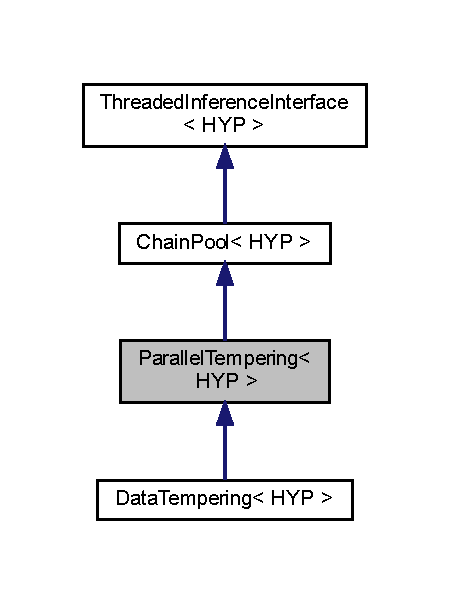
\includegraphics[width=231pt]{class_parallel_tempering__inherit__graph}
\end{center}
\end{figure}


Collaboration diagram for Parallel\+Tempering$<$ H\+YP, callback\+\_\+t $>$\+:
\nopagebreak
\begin{figure}[H]
\begin{center}
\leavevmode
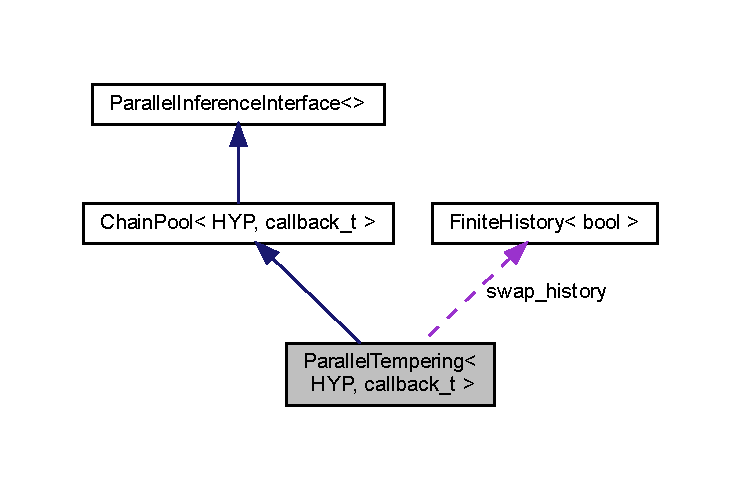
\includegraphics[width=350pt]{class_parallel_tempering__coll__graph}
\end{center}
\end{figure}
\subsection*{Public Member Functions}
\begin{DoxyCompactItemize}
\item 
\hyperlink{class_parallel_tempering_aec98f6abe3a51a3cf79b508ba176d290}{Parallel\+Tempering} (H\+YP \&h0, typename H\+Y\+P\+::data\+\_\+t $\ast$d, callback\+\_\+t \&cb, std\+::initializer\+\_\+list$<$ double $>$ t, bool allcallback=true)
\item 
\hyperlink{class_parallel_tempering_a28bc2e02ad875e2b1cfcde9e428bf97e}{Parallel\+Tempering} (H\+YP \&h0, typename H\+Y\+P\+::data\+\_\+t $\ast$d, callback\+\_\+t \&cb, unsigned long n, double maxT, bool allcallback=true)
\item 
\hyperlink{class_parallel_tempering_a3a186a1ae0f8ed02914d76a7a1dcd229}{Parallel\+Tempering} (H\+YP \&h0, std\+::vector$<$ typename H\+Y\+P\+::data\+\_\+t $>$ \&datas, std\+::vector$<$ callback\+\_\+t $>$ \&cb)
\item 
\hyperlink{class_parallel_tempering_a96763c107a95f4a120f2b65c896cb5b2}{$\sim$\+Parallel\+Tempering} ()
\item 
void \hyperlink{class_parallel_tempering_aa704d462a41cb45b461b967a97dedcbb}{\+\_\+\+\_\+swapper\+\_\+thread} (time\+\_\+ms swap\+\_\+every)
\item 
void \hyperlink{class_parallel_tempering_a6ae6bd8581ec13aad5983886b1a739e6}{\+\_\+\+\_\+adapter\+\_\+thread} (time\+\_\+ms adapt\+\_\+every)
\item 
virtual void \hyperlink{class_parallel_tempering_a6824837893cf52eb1cac362e78e483b9}{run} (\hyperlink{struct_control}{Control} ctl) override
\item 
virtual void \hyperlink{class_parallel_tempering_a40df4781b1d06acff7b0902c4d4a5a87}{run} (\hyperlink{struct_control}{Control} ctl, time\+\_\+ms swap\+\_\+every, time\+\_\+ms adapt\+\_\+every)
\item 
void \hyperlink{class_parallel_tempering_a9e1960158b12a4dadfab54eb4fb895d3}{show\+\_\+statistics} ()
\item 
double \hyperlink{class_parallel_tempering_a439c50d3f616319803d4ab83804d1ae0}{k} (unsigned long t, double v, double t0)
\item 
void \hyperlink{class_parallel_tempering_a673feff316b65cad63f56ceb81b128ae}{adapt} (double v=3, double t0=1000000)
\end{DoxyCompactItemize}
\subsection*{Public Attributes}
\begin{DoxyCompactItemize}
\item 
std\+::vector$<$ double $>$ \hyperlink{class_parallel_tempering_a5aca1e6ca522986f183d61c91c94d21d}{temperatures}
\item 
\hyperlink{class_fleet_1_1_statistics_1_1_finite_history}{Fleet\+::\+Statistics\+::\+Finite\+History}$<$ bool $>$ $\ast$ \hyperlink{class_parallel_tempering_a86a7b77250a04b5df502f1c770cf51bf}{swap\+\_\+history}
\item 
bool \hyperlink{class_parallel_tempering_ae9f0a2af938df838cc4010983860394e}{is\+\_\+temperature}
\item 
std\+::atomic$<$ bool $>$ \hyperlink{class_parallel_tempering_acda523b375468743e7d8ac471af65285}{terminate}
\end{DoxyCompactItemize}
\subsection*{Additional Inherited Members}


\subsection{Constructor \& Destructor Documentation}
\mbox{\Hypertarget{class_parallel_tempering_aec98f6abe3a51a3cf79b508ba176d290}\label{class_parallel_tempering_aec98f6abe3a51a3cf79b508ba176d290}} 
\index{Parallel\+Tempering@{Parallel\+Tempering}!Parallel\+Tempering@{Parallel\+Tempering}}
\index{Parallel\+Tempering@{Parallel\+Tempering}!Parallel\+Tempering@{Parallel\+Tempering}}
\subsubsection{\texorpdfstring{Parallel\+Tempering()}{ParallelTempering()}\hspace{0.1cm}{\footnotesize\ttfamily [1/3]}}
{\footnotesize\ttfamily template$<$typename H\+YP , typename callback\+\_\+t $>$ \\
\hyperlink{class_parallel_tempering}{Parallel\+Tempering}$<$ H\+YP, callback\+\_\+t $>$\+::\hyperlink{class_parallel_tempering}{Parallel\+Tempering} (\begin{DoxyParamCaption}\item[{H\+YP \&}]{h0,  }\item[{typename H\+Y\+P\+::data\+\_\+t $\ast$}]{d,  }\item[{callback\+\_\+t \&}]{cb,  }\item[{std\+::initializer\+\_\+list$<$ double $>$}]{t,  }\item[{bool}]{allcallback = {\ttfamily true} }\end{DoxyParamCaption})\hspace{0.3cm}{\ttfamily [inline]}}

\mbox{\Hypertarget{class_parallel_tempering_a28bc2e02ad875e2b1cfcde9e428bf97e}\label{class_parallel_tempering_a28bc2e02ad875e2b1cfcde9e428bf97e}} 
\index{Parallel\+Tempering@{Parallel\+Tempering}!Parallel\+Tempering@{Parallel\+Tempering}}
\index{Parallel\+Tempering@{Parallel\+Tempering}!Parallel\+Tempering@{Parallel\+Tempering}}
\subsubsection{\texorpdfstring{Parallel\+Tempering()}{ParallelTempering()}\hspace{0.1cm}{\footnotesize\ttfamily [2/3]}}
{\footnotesize\ttfamily template$<$typename H\+YP , typename callback\+\_\+t $>$ \\
\hyperlink{class_parallel_tempering}{Parallel\+Tempering}$<$ H\+YP, callback\+\_\+t $>$\+::\hyperlink{class_parallel_tempering}{Parallel\+Tempering} (\begin{DoxyParamCaption}\item[{H\+YP \&}]{h0,  }\item[{typename H\+Y\+P\+::data\+\_\+t $\ast$}]{d,  }\item[{callback\+\_\+t \&}]{cb,  }\item[{unsigned long}]{n,  }\item[{double}]{maxT,  }\item[{bool}]{allcallback = {\ttfamily true} }\end{DoxyParamCaption})\hspace{0.3cm}{\ttfamily [inline]}}

\mbox{\Hypertarget{class_parallel_tempering_a3a186a1ae0f8ed02914d76a7a1dcd229}\label{class_parallel_tempering_a3a186a1ae0f8ed02914d76a7a1dcd229}} 
\index{Parallel\+Tempering@{Parallel\+Tempering}!Parallel\+Tempering@{Parallel\+Tempering}}
\index{Parallel\+Tempering@{Parallel\+Tempering}!Parallel\+Tempering@{Parallel\+Tempering}}
\subsubsection{\texorpdfstring{Parallel\+Tempering()}{ParallelTempering()}\hspace{0.1cm}{\footnotesize\ttfamily [3/3]}}
{\footnotesize\ttfamily template$<$typename H\+YP , typename callback\+\_\+t $>$ \\
\hyperlink{class_parallel_tempering}{Parallel\+Tempering}$<$ H\+YP, callback\+\_\+t $>$\+::\hyperlink{class_parallel_tempering}{Parallel\+Tempering} (\begin{DoxyParamCaption}\item[{H\+YP \&}]{h0,  }\item[{std\+::vector$<$ typename H\+Y\+P\+::data\+\_\+t $>$ \&}]{datas,  }\item[{std\+::vector$<$ callback\+\_\+t $>$ \&}]{cb }\end{DoxyParamCaption})\hspace{0.3cm}{\ttfamily [inline]}}

\mbox{\Hypertarget{class_parallel_tempering_a96763c107a95f4a120f2b65c896cb5b2}\label{class_parallel_tempering_a96763c107a95f4a120f2b65c896cb5b2}} 
\index{Parallel\+Tempering@{Parallel\+Tempering}!````~Parallel\+Tempering@{$\sim$\+Parallel\+Tempering}}
\index{````~Parallel\+Tempering@{$\sim$\+Parallel\+Tempering}!Parallel\+Tempering@{Parallel\+Tempering}}
\subsubsection{\texorpdfstring{$\sim$\+Parallel\+Tempering()}{~ParallelTempering()}}
{\footnotesize\ttfamily template$<$typename H\+YP , typename callback\+\_\+t $>$ \\
\hyperlink{class_parallel_tempering}{Parallel\+Tempering}$<$ H\+YP, callback\+\_\+t $>$\+::$\sim$\hyperlink{class_parallel_tempering}{Parallel\+Tempering} (\begin{DoxyParamCaption}{ }\end{DoxyParamCaption})\hspace{0.3cm}{\ttfamily [inline]}}



\subsection{Member Function Documentation}
\mbox{\Hypertarget{class_parallel_tempering_a6ae6bd8581ec13aad5983886b1a739e6}\label{class_parallel_tempering_a6ae6bd8581ec13aad5983886b1a739e6}} 
\index{Parallel\+Tempering@{Parallel\+Tempering}!\+\_\+\+\_\+adapter\+\_\+thread@{\+\_\+\+\_\+adapter\+\_\+thread}}
\index{\+\_\+\+\_\+adapter\+\_\+thread@{\+\_\+\+\_\+adapter\+\_\+thread}!Parallel\+Tempering@{Parallel\+Tempering}}
\subsubsection{\texorpdfstring{\+\_\+\+\_\+adapter\+\_\+thread()}{\_\_adapter\_thread()}}
{\footnotesize\ttfamily template$<$typename H\+YP , typename callback\+\_\+t $>$ \\
void \hyperlink{class_parallel_tempering}{Parallel\+Tempering}$<$ H\+YP, callback\+\_\+t $>$\+::\+\_\+\+\_\+adapter\+\_\+thread (\begin{DoxyParamCaption}\item[{time\+\_\+ms}]{adapt\+\_\+every }\end{DoxyParamCaption})\hspace{0.3cm}{\ttfamily [inline]}}

\mbox{\Hypertarget{class_parallel_tempering_aa704d462a41cb45b461b967a97dedcbb}\label{class_parallel_tempering_aa704d462a41cb45b461b967a97dedcbb}} 
\index{Parallel\+Tempering@{Parallel\+Tempering}!\+\_\+\+\_\+swapper\+\_\+thread@{\+\_\+\+\_\+swapper\+\_\+thread}}
\index{\+\_\+\+\_\+swapper\+\_\+thread@{\+\_\+\+\_\+swapper\+\_\+thread}!Parallel\+Tempering@{Parallel\+Tempering}}
\subsubsection{\texorpdfstring{\+\_\+\+\_\+swapper\+\_\+thread()}{\_\_swapper\_thread()}}
{\footnotesize\ttfamily template$<$typename H\+YP , typename callback\+\_\+t $>$ \\
void \hyperlink{class_parallel_tempering}{Parallel\+Tempering}$<$ H\+YP, callback\+\_\+t $>$\+::\+\_\+\+\_\+swapper\+\_\+thread (\begin{DoxyParamCaption}\item[{time\+\_\+ms}]{swap\+\_\+every }\end{DoxyParamCaption})\hspace{0.3cm}{\ttfamily [inline]}}

\mbox{\Hypertarget{class_parallel_tempering_a673feff316b65cad63f56ceb81b128ae}\label{class_parallel_tempering_a673feff316b65cad63f56ceb81b128ae}} 
\index{Parallel\+Tempering@{Parallel\+Tempering}!adapt@{adapt}}
\index{adapt@{adapt}!Parallel\+Tempering@{Parallel\+Tempering}}
\subsubsection{\texorpdfstring{adapt()}{adapt()}}
{\footnotesize\ttfamily template$<$typename H\+YP , typename callback\+\_\+t $>$ \\
void \hyperlink{class_parallel_tempering}{Parallel\+Tempering}$<$ H\+YP, callback\+\_\+t $>$\+::adapt (\begin{DoxyParamCaption}\item[{double}]{v = {\ttfamily 3},  }\item[{double}]{t0 = {\ttfamily 1000000} }\end{DoxyParamCaption})\hspace{0.3cm}{\ttfamily [inline]}}

\mbox{\Hypertarget{class_parallel_tempering_a439c50d3f616319803d4ab83804d1ae0}\label{class_parallel_tempering_a439c50d3f616319803d4ab83804d1ae0}} 
\index{Parallel\+Tempering@{Parallel\+Tempering}!k@{k}}
\index{k@{k}!Parallel\+Tempering@{Parallel\+Tempering}}
\subsubsection{\texorpdfstring{k()}{k()}}
{\footnotesize\ttfamily template$<$typename H\+YP , typename callback\+\_\+t $>$ \\
double \hyperlink{class_parallel_tempering}{Parallel\+Tempering}$<$ H\+YP, callback\+\_\+t $>$\+::k (\begin{DoxyParamCaption}\item[{unsigned long}]{t,  }\item[{double}]{v,  }\item[{double}]{t0 }\end{DoxyParamCaption})\hspace{0.3cm}{\ttfamily [inline]}}

\mbox{\Hypertarget{class_parallel_tempering_a6824837893cf52eb1cac362e78e483b9}\label{class_parallel_tempering_a6824837893cf52eb1cac362e78e483b9}} 
\index{Parallel\+Tempering@{Parallel\+Tempering}!run@{run}}
\index{run@{run}!Parallel\+Tempering@{Parallel\+Tempering}}
\subsubsection{\texorpdfstring{run()}{run()}\hspace{0.1cm}{\footnotesize\ttfamily [1/2]}}
{\footnotesize\ttfamily template$<$typename H\+YP , typename callback\+\_\+t $>$ \\
virtual void \hyperlink{class_parallel_tempering}{Parallel\+Tempering}$<$ H\+YP, callback\+\_\+t $>$\+::run (\begin{DoxyParamCaption}\item[{\hyperlink{struct_control}{Control}}]{ctl }\end{DoxyParamCaption})\hspace{0.3cm}{\ttfamily [inline]}, {\ttfamily [override]}, {\ttfamily [virtual]}}



Reimplemented from \hyperlink{class_chain_pool_af5f0e391f9794ff89f29296c8b41bf8e}{Chain\+Pool$<$ H\+Y\+P, callback\+\_\+t $>$}.

\mbox{\Hypertarget{class_parallel_tempering_a40df4781b1d06acff7b0902c4d4a5a87}\label{class_parallel_tempering_a40df4781b1d06acff7b0902c4d4a5a87}} 
\index{Parallel\+Tempering@{Parallel\+Tempering}!run@{run}}
\index{run@{run}!Parallel\+Tempering@{Parallel\+Tempering}}
\subsubsection{\texorpdfstring{run()}{run()}\hspace{0.1cm}{\footnotesize\ttfamily [2/2]}}
{\footnotesize\ttfamily template$<$typename H\+YP , typename callback\+\_\+t $>$ \\
virtual void \hyperlink{class_parallel_tempering}{Parallel\+Tempering}$<$ H\+YP, callback\+\_\+t $>$\+::run (\begin{DoxyParamCaption}\item[{\hyperlink{struct_control}{Control}}]{ctl,  }\item[{time\+\_\+ms}]{swap\+\_\+every,  }\item[{time\+\_\+ms}]{adapt\+\_\+every }\end{DoxyParamCaption})\hspace{0.3cm}{\ttfamily [inline]}, {\ttfamily [virtual]}}

\mbox{\Hypertarget{class_parallel_tempering_a9e1960158b12a4dadfab54eb4fb895d3}\label{class_parallel_tempering_a9e1960158b12a4dadfab54eb4fb895d3}} 
\index{Parallel\+Tempering@{Parallel\+Tempering}!show\+\_\+statistics@{show\+\_\+statistics}}
\index{show\+\_\+statistics@{show\+\_\+statistics}!Parallel\+Tempering@{Parallel\+Tempering}}
\subsubsection{\texorpdfstring{show\+\_\+statistics()}{show\_statistics()}}
{\footnotesize\ttfamily template$<$typename H\+YP , typename callback\+\_\+t $>$ \\
void \hyperlink{class_parallel_tempering}{Parallel\+Tempering}$<$ H\+YP, callback\+\_\+t $>$\+::show\+\_\+statistics (\begin{DoxyParamCaption}{ }\end{DoxyParamCaption})\hspace{0.3cm}{\ttfamily [inline]}}



\subsection{Member Data Documentation}
\mbox{\Hypertarget{class_parallel_tempering_ae9f0a2af938df838cc4010983860394e}\label{class_parallel_tempering_ae9f0a2af938df838cc4010983860394e}} 
\index{Parallel\+Tempering@{Parallel\+Tempering}!is\+\_\+temperature@{is\+\_\+temperature}}
\index{is\+\_\+temperature@{is\+\_\+temperature}!Parallel\+Tempering@{Parallel\+Tempering}}
\subsubsection{\texorpdfstring{is\+\_\+temperature}{is\_temperature}}
{\footnotesize\ttfamily template$<$typename H\+YP , typename callback\+\_\+t $>$ \\
bool \hyperlink{class_parallel_tempering}{Parallel\+Tempering}$<$ H\+YP, callback\+\_\+t $>$\+::is\+\_\+temperature}

\mbox{\Hypertarget{class_parallel_tempering_a86a7b77250a04b5df502f1c770cf51bf}\label{class_parallel_tempering_a86a7b77250a04b5df502f1c770cf51bf}} 
\index{Parallel\+Tempering@{Parallel\+Tempering}!swap\+\_\+history@{swap\+\_\+history}}
\index{swap\+\_\+history@{swap\+\_\+history}!Parallel\+Tempering@{Parallel\+Tempering}}
\subsubsection{\texorpdfstring{swap\+\_\+history}{swap\_history}}
{\footnotesize\ttfamily template$<$typename H\+YP , typename callback\+\_\+t $>$ \\
\hyperlink{class_fleet_1_1_statistics_1_1_finite_history}{Fleet\+::\+Statistics\+::\+Finite\+History}$<$bool$>$$\ast$ \hyperlink{class_parallel_tempering}{Parallel\+Tempering}$<$ H\+YP, callback\+\_\+t $>$\+::swap\+\_\+history}

\mbox{\Hypertarget{class_parallel_tempering_a5aca1e6ca522986f183d61c91c94d21d}\label{class_parallel_tempering_a5aca1e6ca522986f183d61c91c94d21d}} 
\index{Parallel\+Tempering@{Parallel\+Tempering}!temperatures@{temperatures}}
\index{temperatures@{temperatures}!Parallel\+Tempering@{Parallel\+Tempering}}
\subsubsection{\texorpdfstring{temperatures}{temperatures}}
{\footnotesize\ttfamily template$<$typename H\+YP , typename callback\+\_\+t $>$ \\
std\+::vector$<$double$>$ \hyperlink{class_parallel_tempering}{Parallel\+Tempering}$<$ H\+YP, callback\+\_\+t $>$\+::temperatures}

\mbox{\Hypertarget{class_parallel_tempering_acda523b375468743e7d8ac471af65285}\label{class_parallel_tempering_acda523b375468743e7d8ac471af65285}} 
\index{Parallel\+Tempering@{Parallel\+Tempering}!terminate@{terminate}}
\index{terminate@{terminate}!Parallel\+Tempering@{Parallel\+Tempering}}
\subsubsection{\texorpdfstring{terminate}{terminate}}
{\footnotesize\ttfamily template$<$typename H\+YP , typename callback\+\_\+t $>$ \\
std\+::atomic$<$bool$>$ \hyperlink{class_parallel_tempering}{Parallel\+Tempering}$<$ H\+YP, callback\+\_\+t $>$\+::terminate}



The documentation for this class was generated from the following file\+:\begin{DoxyCompactItemize}
\item 
src/\+Inference/\hyperlink{_parallel_tempering_8h}{Parallel\+Tempering.\+h}\end{DoxyCompactItemize}

\hypertarget{class_partial_m_c_t_s_node}{}\doxysection{Partial\+M\+C\+T\+S\+Node$<$ this\+\_\+t, H\+YP, callback\+\_\+t $>$ Class Template Reference}
\label{class_partial_m_c_t_s_node}\index{PartialMCTSNode$<$ this\_t, HYP, callback\_t $>$@{PartialMCTSNode$<$ this\_t, HYP, callback\_t $>$}}


{\ttfamily \#include $<$M\+C\+T\+S.\+h$>$}



Inheritance diagram for Partial\+M\+C\+T\+S\+Node$<$ this\+\_\+t, H\+YP, callback\+\_\+t $>$\+:
\nopagebreak
\begin{figure}[H]
\begin{center}
\leavevmode
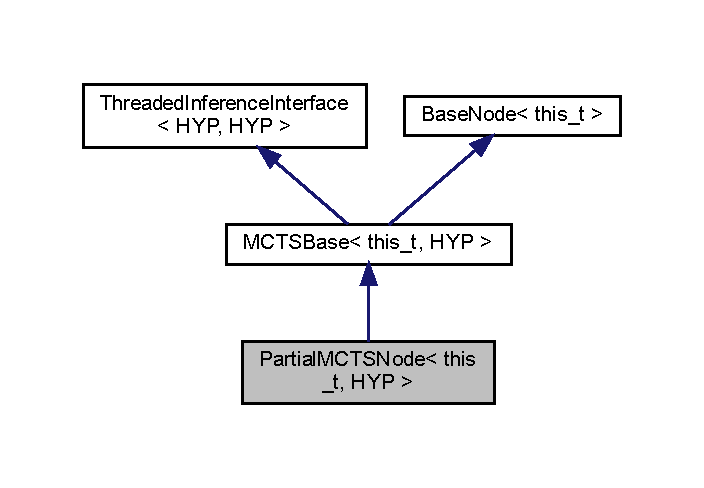
\includegraphics[width=330pt]{class_partial_m_c_t_s_node__inherit__graph}
\end{center}
\end{figure}


Collaboration diagram for Partial\+M\+C\+T\+S\+Node$<$ this\+\_\+t, H\+YP, callback\+\_\+t $>$\+:
\nopagebreak
\begin{figure}[H]
\begin{center}
\leavevmode
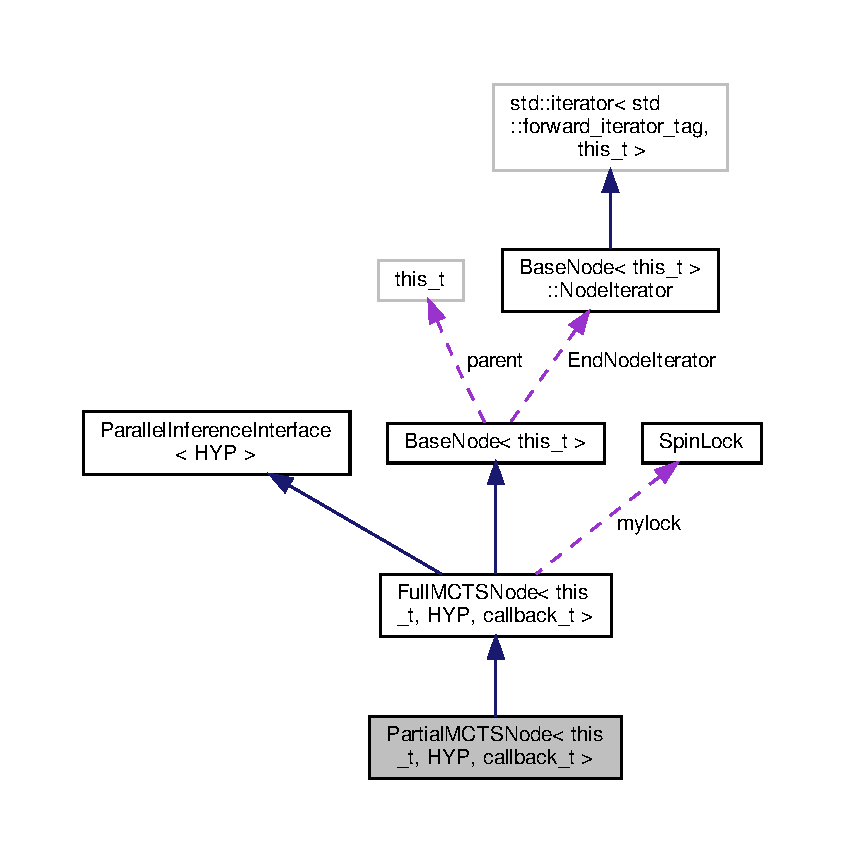
\includegraphics[width=350pt]{class_partial_m_c_t_s_node__coll__graph}
\end{center}
\end{figure}
\doxysubsection*{Friends}
\begin{DoxyCompactItemize}
\item 
class \mbox{\hyperlink{class_partial_m_c_t_s_node_a6f119b2294000202fb5eaa562a7aa52b}{Full\+M\+C\+T\+S\+Node$<$ this\+\_\+t, H\+Y\+P, callback\+\_\+t $>$}}
\end{DoxyCompactItemize}
\doxysubsection*{Additional Inherited Members}


\doxysubsection{Detailed Description}
\subsubsection*{template$<$typename this\+\_\+t, typename H\+YP, typename callback\+\_\+t$>$\newline
class Partial\+M\+C\+T\+S\+Node$<$ this\+\_\+t, H\+Y\+P, callback\+\_\+t $>$}

\begin{DoxyAuthor}{Author}
piantado 
\end{DoxyAuthor}
\begin{DoxyDate}{Date}
03/07/20 
\end{DoxyDate}


\doxysubsection{Friends And Related Function Documentation}
\mbox{\Hypertarget{class_partial_m_c_t_s_node_a6f119b2294000202fb5eaa562a7aa52b}\label{class_partial_m_c_t_s_node_a6f119b2294000202fb5eaa562a7aa52b}} 
\index{PartialMCTSNode$<$ this\_t, HYP, callback\_t $>$@{PartialMCTSNode$<$ this\_t, HYP, callback\_t $>$}!FullMCTSNode$<$ this\_t, HYP, callback\_t $>$@{FullMCTSNode$<$ this\_t, HYP, callback\_t $>$}}
\index{FullMCTSNode$<$ this\_t, HYP, callback\_t $>$@{FullMCTSNode$<$ this\_t, HYP, callback\_t $>$}!PartialMCTSNode$<$ this\_t, HYP, callback\_t $>$@{PartialMCTSNode$<$ this\_t, HYP, callback\_t $>$}}
\doxysubsubsection{\texorpdfstring{FullMCTSNode$<$ this\_t, HYP, callback\_t $>$}{FullMCTSNode< this\_t, HYP, callback\_t >}}
{\footnotesize\ttfamily template$<$typename this\+\_\+t , typename H\+YP , typename callback\+\_\+t $>$ \\
friend class \mbox{\hyperlink{class_full_m_c_t_s_node}{Full\+M\+C\+T\+S\+Node}}$<$ this\+\_\+t, H\+YP, callback\+\_\+t $>$\hspace{0.3cm}{\ttfamily [friend]}}



The documentation for this class was generated from the following file\+:\begin{DoxyCompactItemize}
\item 
src/\+Inference/\mbox{\hyperlink{_m_c_t_s_8h}{M\+C\+T\+S.\+h}}\end{DoxyCompactItemize}

\hypertarget{struct_pre_primitive}{}\doxysection{Pre\+Primitive Class Reference}
\label{struct_pre_primitive}\index{PrePrimitive@{PrePrimitive}}


{\ttfamily \#include $<$Primitives.\+h$>$}

\doxysubsection*{Static Public Attributes}
\begin{DoxyCompactItemize}
\item 
static \mbox{\hyperlink{_instruction_8h_a227278394efd1e2313c727102db09ea9}{Primitive\+Op}} \mbox{\hyperlink{struct_pre_primitive_a8f4088dc0a3fe00fd81c509bb0af1881}{op\+\_\+counter}} = 0
\end{DoxyCompactItemize}


\doxysubsection{Detailed Description}
\begin{DoxyAuthor}{Author}
piantado 
\end{DoxyAuthor}
\begin{DoxyDate}{Date}
05/03/20 
\end{DoxyDate}


\doxysubsection{Member Data Documentation}
\mbox{\Hypertarget{struct_pre_primitive_a8f4088dc0a3fe00fd81c509bb0af1881}\label{struct_pre_primitive_a8f4088dc0a3fe00fd81c509bb0af1881}} 
\index{PrePrimitive@{PrePrimitive}!op\_counter@{op\_counter}}
\index{op\_counter@{op\_counter}!PrePrimitive@{PrePrimitive}}
\doxysubsubsection{\texorpdfstring{op\_counter}{op\_counter}}
{\footnotesize\ttfamily \mbox{\hyperlink{_instruction_8h_a227278394efd1e2313c727102db09ea9}{Primitive\+Op}} Pre\+Primitive\+::op\+\_\+counter = 0\hspace{0.3cm}{\ttfamily [static]}}



The documentation for this class was generated from the following file\+:\begin{DoxyCompactItemize}
\item 
src/\+Virtual\+Machine/\mbox{\hyperlink{_primitives_8h}{Primitives.\+h}}\end{DoxyCompactItemize}

\hypertarget{struct_primitive}{}\section{Primitive$<$ T, args $>$ Class Template Reference}
\label{struct_primitive}\index{Primitive$<$ T, args $>$@{Primitive$<$ T, args $>$}}


{\ttfamily \#include $<$Grammar.\+h$>$}



Inheritance diagram for Primitive$<$ T, args $>$\+:
\nopagebreak
\begin{figure}[H]
\begin{center}
\leavevmode
\includegraphics[width=184pt]{struct_primitive__inherit__graph}
\end{center}
\end{figure}


Collaboration diagram for Primitive$<$ T, args $>$\+:
\nopagebreak
\begin{figure}[H]
\begin{center}
\leavevmode
\includegraphics[width=184pt]{struct_primitive__coll__graph}
\end{center}
\end{figure}
\subsection*{Public Types}
\begin{DoxyCompactItemize}
\item 
typedef std\+::decay$<$ typename \hyperlink{struct_head_if_reference_else_t}{Head\+If\+Reference\+ElseT}$<$ T, args... $>$\+::type $>$\+::type \hyperlink{struct_primitive_a1f2d2db3fb7869d03d65112e30d22101}{Grammar\+Return\+Type}
\end{DoxyCompactItemize}
\subsection*{Public Member Functions}
\begin{DoxyCompactItemize}
\item 
constexpr \hyperlink{struct_primitive_a582a781e02c86b17df208d6fc0c39daf}{Primitive} (const char $\ast$fmt, T($\ast$\+\_\+call)(args...), double \+\_\+p=1.\+0)
\item 
{\footnotesize template$<$typename V , typename P , typename L $>$ }\\constexpr \hyperlink{struct_primitive_a8a9ad9e0b9c7bc94bbb4290cb298288c}{Primitive} (const char $\ast$fmt, T($\ast$\+\_\+call)(args...), \hyperlink{_instruction_8h_a6202215407ab29590bb936ca2996cf64}{vmstatus\+\_\+t} \+\_\+dispatch(V $\ast$, P $\ast$, L $\ast$), double \+\_\+p=1.\+0)
\item 
{\footnotesize template$<$typename V , typename P , typename L $>$ }\\\hyperlink{_instruction_8h_a6202215407ab29590bb936ca2996cf64}{vmstatus\+\_\+t} \hyperlink{struct_primitive_a10cedec90ed4a3ff01be2bd3b9c36528}{V\+M\+Scall} (V $\ast$vms, P $\ast$pool, L $\ast$loader)
\begin{DoxyCompactList}\small\item\em This gets called by a \hyperlink{class_virtual_machine_state}{Virtual\+Machine\+State} to evaluate the primitive on some arguments. \end{DoxyCompactList}\end{DoxyCompactItemize}
\subsection*{Public Attributes}
\begin{DoxyCompactItemize}
\item 
std\+::string \hyperlink{struct_primitive_afa8c2d4087b36ae9580fed3dc00e47b6}{format}
\item 
T($\ast$ \hyperlink{struct_primitive_a4a183f50daf033866abc34fa2da9e703}{call} )(args...)
\item 
std\+::any \hyperlink{struct_primitive_a8fe52297e3da666ec08e2328a3fe92e9}{dispatch}
\item 
\hyperlink{_instruction_8h_a227278394efd1e2313c727102db09ea9}{Primitive\+Op} \hyperlink{struct_primitive_a45ef953a37468a97b5a4b5531e5f21ce}{op}
\item 
double \hyperlink{struct_primitive_a43fac47ebf8ec63a70443d80dcd04687}{p}
\item 
bool \hyperlink{struct_primitive_a599bf4b9b5115d99c203b51dc028ba4e}{is\+\_\+dispatch}
\end{DoxyCompactItemize}
\subsection*{Additional Inherited Members}


\subsection{Detailed Description}
\subsubsection*{template$<$typename T, typename... args$>$\newline
class Primitive$<$ T, args $>$}

\begin{DoxyAuthor}{Author}
piantado 
\end{DoxyAuthor}
\begin{DoxyDate}{Date}
05/03/20 
\end{DoxyDate}


\subsection{Member Typedef Documentation}
\mbox{\Hypertarget{struct_primitive_a1f2d2db3fb7869d03d65112e30d22101}\label{struct_primitive_a1f2d2db3fb7869d03d65112e30d22101}} 
\index{Primitive@{Primitive}!Grammar\+Return\+Type@{Grammar\+Return\+Type}}
\index{Grammar\+Return\+Type@{Grammar\+Return\+Type}!Primitive@{Primitive}}
\subsubsection{\texorpdfstring{Grammar\+Return\+Type}{GrammarReturnType}}
{\footnotesize\ttfamily template$<$typename T, typename... args$>$ \\
typedef std\+::decay$<$typename \hyperlink{struct_head_if_reference_else_t}{Head\+If\+Reference\+ElseT}$<$T,args...$>$\+::type$>$\+::type \hyperlink{struct_primitive}{Primitive}$<$ T, args $>$\+::\hyperlink{struct_primitive_a1f2d2db3fb7869d03d65112e30d22101}{Grammar\+Return\+Type}}



\subsection{Constructor \& Destructor Documentation}
\mbox{\Hypertarget{struct_primitive_a582a781e02c86b17df208d6fc0c39daf}\label{struct_primitive_a582a781e02c86b17df208d6fc0c39daf}} 
\index{Primitive@{Primitive}!Primitive@{Primitive}}
\index{Primitive@{Primitive}!Primitive@{Primitive}}
\subsubsection{\texorpdfstring{Primitive()}{Primitive()}\hspace{0.1cm}{\footnotesize\ttfamily [1/2]}}
{\footnotesize\ttfamily template$<$typename T, typename... args$>$ \\
constexpr \hyperlink{struct_primitive}{Primitive}$<$ T, args $>$\+::\hyperlink{struct_primitive}{Primitive} (\begin{DoxyParamCaption}\item[{const char $\ast$}]{fmt,  }\item[{T($\ast$)(args...)}]{\+\_\+call,  }\item[{double}]{\+\_\+p = {\ttfamily 1.0} }\end{DoxyParamCaption})\hspace{0.3cm}{\ttfamily [inline]}}

\mbox{\Hypertarget{struct_primitive_a8a9ad9e0b9c7bc94bbb4290cb298288c}\label{struct_primitive_a8a9ad9e0b9c7bc94bbb4290cb298288c}} 
\index{Primitive@{Primitive}!Primitive@{Primitive}}
\index{Primitive@{Primitive}!Primitive@{Primitive}}
\subsubsection{\texorpdfstring{Primitive()}{Primitive()}\hspace{0.1cm}{\footnotesize\ttfamily [2/2]}}
{\footnotesize\ttfamily template$<$typename T, typename... args$>$ \\
template$<$typename V , typename P , typename L $>$ \\
constexpr \hyperlink{struct_primitive}{Primitive}$<$ T, args $>$\+::\hyperlink{struct_primitive}{Primitive} (\begin{DoxyParamCaption}\item[{const char $\ast$}]{fmt,  }\item[{T($\ast$)(args...)}]{\+\_\+call,  }\item[{\hyperlink{_instruction_8h_a6202215407ab29590bb936ca2996cf64}{vmstatus\+\_\+t} }]{\+\_\+dispatchV $\ast$, P $\ast$, L $\ast$,  }\item[{double}]{\+\_\+p = {\ttfamily 1.0} }\end{DoxyParamCaption})\hspace{0.3cm}{\ttfamily [inline]}}



\subsection{Member Function Documentation}
\mbox{\Hypertarget{struct_primitive_a10cedec90ed4a3ff01be2bd3b9c36528}\label{struct_primitive_a10cedec90ed4a3ff01be2bd3b9c36528}} 
\index{Primitive@{Primitive}!V\+M\+Scall@{V\+M\+Scall}}
\index{V\+M\+Scall@{V\+M\+Scall}!Primitive@{Primitive}}
\subsubsection{\texorpdfstring{V\+M\+Scall()}{VMScall()}}
{\footnotesize\ttfamily template$<$typename T, typename... args$>$ \\
template$<$typename V , typename P , typename L $>$ \\
\hyperlink{_instruction_8h_a6202215407ab29590bb936ca2996cf64}{vmstatus\+\_\+t} \hyperlink{struct_primitive}{Primitive}$<$ T, args $>$\+::V\+M\+Scall (\begin{DoxyParamCaption}\item[{V $\ast$}]{vms,  }\item[{P $\ast$}]{pool,  }\item[{L $\ast$}]{loader }\end{DoxyParamCaption})\hspace{0.3cm}{\ttfamily [inline]}}



This gets called by a \hyperlink{class_virtual_machine_state}{Virtual\+Machine\+State} to evaluate the primitive on some arguments. 


\begin{DoxyParams}{Parameters}
{\em vms} & \\
\hline
{\em pool} & \\
\hline
{\em loader} & \\
\hline
\end{DoxyParams}
\begin{DoxyReturn}{Returns}

\end{DoxyReturn}


\subsection{Member Data Documentation}
\mbox{\Hypertarget{struct_primitive_a4a183f50daf033866abc34fa2da9e703}\label{struct_primitive_a4a183f50daf033866abc34fa2da9e703}} 
\index{Primitive@{Primitive}!call@{call}}
\index{call@{call}!Primitive@{Primitive}}
\subsubsection{\texorpdfstring{call}{call}}
{\footnotesize\ttfamily template$<$typename T, typename... args$>$ \\
T($\ast$ \hyperlink{struct_primitive}{Primitive}$<$ T, args $>$\+::call) (args...)}

\mbox{\Hypertarget{struct_primitive_a8fe52297e3da666ec08e2328a3fe92e9}\label{struct_primitive_a8fe52297e3da666ec08e2328a3fe92e9}} 
\index{Primitive@{Primitive}!dispatch@{dispatch}}
\index{dispatch@{dispatch}!Primitive@{Primitive}}
\subsubsection{\texorpdfstring{dispatch}{dispatch}}
{\footnotesize\ttfamily template$<$typename T, typename... args$>$ \\
std\+::any \hyperlink{struct_primitive}{Primitive}$<$ T, args $>$\+::dispatch}

\mbox{\Hypertarget{struct_primitive_afa8c2d4087b36ae9580fed3dc00e47b6}\label{struct_primitive_afa8c2d4087b36ae9580fed3dc00e47b6}} 
\index{Primitive@{Primitive}!format@{format}}
\index{format@{format}!Primitive@{Primitive}}
\subsubsection{\texorpdfstring{format}{format}}
{\footnotesize\ttfamily template$<$typename T, typename... args$>$ \\
std\+::string \hyperlink{struct_primitive}{Primitive}$<$ T, args $>$\+::format}

\mbox{\Hypertarget{struct_primitive_a599bf4b9b5115d99c203b51dc028ba4e}\label{struct_primitive_a599bf4b9b5115d99c203b51dc028ba4e}} 
\index{Primitive@{Primitive}!is\+\_\+dispatch@{is\+\_\+dispatch}}
\index{is\+\_\+dispatch@{is\+\_\+dispatch}!Primitive@{Primitive}}
\subsubsection{\texorpdfstring{is\+\_\+dispatch}{is\_dispatch}}
{\footnotesize\ttfamily template$<$typename T, typename... args$>$ \\
bool \hyperlink{struct_primitive}{Primitive}$<$ T, args $>$\+::is\+\_\+dispatch}

\mbox{\Hypertarget{struct_primitive_a45ef953a37468a97b5a4b5531e5f21ce}\label{struct_primitive_a45ef953a37468a97b5a4b5531e5f21ce}} 
\index{Primitive@{Primitive}!op@{op}}
\index{op@{op}!Primitive@{Primitive}}
\subsubsection{\texorpdfstring{op}{op}}
{\footnotesize\ttfamily template$<$typename T, typename... args$>$ \\
\hyperlink{_instruction_8h_a227278394efd1e2313c727102db09ea9}{Primitive\+Op} \hyperlink{struct_primitive}{Primitive}$<$ T, args $>$\+::op}

\mbox{\Hypertarget{struct_primitive_a43fac47ebf8ec63a70443d80dcd04687}\label{struct_primitive_a43fac47ebf8ec63a70443d80dcd04687}} 
\index{Primitive@{Primitive}!p@{p}}
\index{p@{p}!Primitive@{Primitive}}
\subsubsection{\texorpdfstring{p}{p}}
{\footnotesize\ttfamily template$<$typename T, typename... args$>$ \\
double \hyperlink{struct_primitive}{Primitive}$<$ T, args $>$\+::p}



The documentation for this class was generated from the following files\+:\begin{DoxyCompactItemize}
\item 
src/\+Grammar/\hyperlink{_grammar_8h}{Grammar.\+h}\item 
src/\+Virtual\+Machine/\hyperlink{_primitives_8h}{Primitives.\+h}\end{DoxyCompactItemize}

\hypertarget{class_prior_inference}{}\doxysection{Prior\+Inference$<$ H\+YP, callback\+\_\+t $>$ Class Template Reference}
\label{class_prior_inference}\index{PriorInference$<$ HYP, callback\_t $>$@{PriorInference$<$ HYP, callback\_t $>$}}


{\ttfamily \#include $<$Prior\+Inference.\+h$>$}



Inheritance diagram for Prior\+Inference$<$ H\+YP, callback\+\_\+t $>$\+:
\nopagebreak
\begin{figure}[H]
\begin{center}
\leavevmode
\includegraphics[width=208pt]{class_prior_inference__inherit__graph}
\end{center}
\end{figure}


Collaboration diagram for Prior\+Inference$<$ H\+YP, callback\+\_\+t $>$\+:
\nopagebreak
\begin{figure}[H]
\begin{center}
\leavevmode
\includegraphics[width=208pt]{class_prior_inference__coll__graph}
\end{center}
\end{figure}
\doxysubsection*{Public Member Functions}
\begin{DoxyCompactItemize}
\item 
\mbox{\hyperlink{class_prior_inference_ad6ccd45888ca5616f03daed5dd0a1139}{Prior\+Inference}} (Grammar\+\_\+t $\ast$g, \mbox{\hyperlink{_nonterminal_8h_a1c5bfe9b903f69c83bbde5da7035fef3}{nonterminal\+\_\+t}} st, typename H\+Y\+P\+::data\+\_\+t $\ast$d, callback\+\_\+t \&cb)
\item 
void \mbox{\hyperlink{class_prior_inference_a1c641618dffc7d3182ffdb2451500c01}{run\+\_\+thread}} (\mbox{\hyperlink{struct_control}{Control}} ctl) override
\end{DoxyCompactItemize}
\doxysubsection*{Public Attributes}
\begin{DoxyCompactItemize}
\item 
Grammar\+\_\+t $\ast$ \mbox{\hyperlink{class_prior_inference_abafbe828a4c4a98d3828c65e9826fab6}{grammar}}
\item 
\mbox{\hyperlink{_nonterminal_8h_a1c5bfe9b903f69c83bbde5da7035fef3}{nonterminal\+\_\+t}} \mbox{\hyperlink{class_prior_inference_ab5732461e8c514eebc2c29b3d19e4cd1}{start}}
\item 
H\+Y\+P\+::data\+\_\+t $\ast$ \mbox{\hyperlink{class_prior_inference_a537a489d953992aca5327899548df8ac}{data}}
\item 
callback\+\_\+t $\ast$ \mbox{\hyperlink{class_prior_inference_a0b71e0bf3b2c27fa97be006a3c3738a0}{callback}}
\end{DoxyCompactItemize}


\doxysubsection{Detailed Description}
\subsubsection*{template$<$typename H\+YP, typename callback\+\_\+t$>$\newline
class Prior\+Inference$<$ H\+Y\+P, callback\+\_\+t $>$}

\begin{DoxyAuthor}{Author}
piantado 
\end{DoxyAuthor}
\begin{DoxyDate}{Date}
10/06/20 
\end{DoxyDate}


\doxysubsection{Constructor \& Destructor Documentation}
\mbox{\Hypertarget{class_prior_inference_ad6ccd45888ca5616f03daed5dd0a1139}\label{class_prior_inference_ad6ccd45888ca5616f03daed5dd0a1139}} 
\index{PriorInference$<$ HYP, callback\_t $>$@{PriorInference$<$ HYP, callback\_t $>$}!PriorInference@{PriorInference}}
\index{PriorInference@{PriorInference}!PriorInference$<$ HYP, callback\_t $>$@{PriorInference$<$ HYP, callback\_t $>$}}
\doxysubsubsection{\texorpdfstring{PriorInference()}{PriorInference()}}
{\footnotesize\ttfamily template$<$typename H\+YP , typename callback\+\_\+t $>$ \\
\mbox{\hyperlink{class_prior_inference}{Prior\+Inference}}$<$ H\+YP, callback\+\_\+t $>$\+::\mbox{\hyperlink{class_prior_inference}{Prior\+Inference}} (\begin{DoxyParamCaption}\item[{Grammar\+\_\+t $\ast$}]{g,  }\item[{\mbox{\hyperlink{_nonterminal_8h_a1c5bfe9b903f69c83bbde5da7035fef3}{nonterminal\+\_\+t}}}]{st,  }\item[{typename H\+Y\+P\+::data\+\_\+t $\ast$}]{d,  }\item[{callback\+\_\+t \&}]{cb }\end{DoxyParamCaption})\hspace{0.3cm}{\ttfamily [inline]}}



\doxysubsection{Member Function Documentation}
\mbox{\Hypertarget{class_prior_inference_a1c641618dffc7d3182ffdb2451500c01}\label{class_prior_inference_a1c641618dffc7d3182ffdb2451500c01}} 
\index{PriorInference$<$ HYP, callback\_t $>$@{PriorInference$<$ HYP, callback\_t $>$}!run\_thread@{run\_thread}}
\index{run\_thread@{run\_thread}!PriorInference$<$ HYP, callback\_t $>$@{PriorInference$<$ HYP, callback\_t $>$}}
\doxysubsubsection{\texorpdfstring{run\_thread()}{run\_thread()}}
{\footnotesize\ttfamily template$<$typename H\+YP , typename callback\+\_\+t $>$ \\
void \mbox{\hyperlink{class_prior_inference}{Prior\+Inference}}$<$ H\+YP, callback\+\_\+t $>$\+::run\+\_\+thread (\begin{DoxyParamCaption}\item[{\mbox{\hyperlink{struct_control}{Control}}}]{ctl }\end{DoxyParamCaption})\hspace{0.3cm}{\ttfamily [inline]}, {\ttfamily [override]}}



\doxysubsection{Member Data Documentation}
\mbox{\Hypertarget{class_prior_inference_a0b71e0bf3b2c27fa97be006a3c3738a0}\label{class_prior_inference_a0b71e0bf3b2c27fa97be006a3c3738a0}} 
\index{PriorInference$<$ HYP, callback\_t $>$@{PriorInference$<$ HYP, callback\_t $>$}!callback@{callback}}
\index{callback@{callback}!PriorInference$<$ HYP, callback\_t $>$@{PriorInference$<$ HYP, callback\_t $>$}}
\doxysubsubsection{\texorpdfstring{callback}{callback}}
{\footnotesize\ttfamily template$<$typename H\+YP , typename callback\+\_\+t $>$ \\
callback\+\_\+t$\ast$ \mbox{\hyperlink{class_prior_inference}{Prior\+Inference}}$<$ H\+YP, callback\+\_\+t $>$\+::callback}

\mbox{\Hypertarget{class_prior_inference_a537a489d953992aca5327899548df8ac}\label{class_prior_inference_a537a489d953992aca5327899548df8ac}} 
\index{PriorInference$<$ HYP, callback\_t $>$@{PriorInference$<$ HYP, callback\_t $>$}!data@{data}}
\index{data@{data}!PriorInference$<$ HYP, callback\_t $>$@{PriorInference$<$ HYP, callback\_t $>$}}
\doxysubsubsection{\texorpdfstring{data}{data}}
{\footnotesize\ttfamily template$<$typename H\+YP , typename callback\+\_\+t $>$ \\
H\+Y\+P\+::data\+\_\+t$\ast$ \mbox{\hyperlink{class_prior_inference}{Prior\+Inference}}$<$ H\+YP, callback\+\_\+t $>$\+::data}

\mbox{\Hypertarget{class_prior_inference_abafbe828a4c4a98d3828c65e9826fab6}\label{class_prior_inference_abafbe828a4c4a98d3828c65e9826fab6}} 
\index{PriorInference$<$ HYP, callback\_t $>$@{PriorInference$<$ HYP, callback\_t $>$}!grammar@{grammar}}
\index{grammar@{grammar}!PriorInference$<$ HYP, callback\_t $>$@{PriorInference$<$ HYP, callback\_t $>$}}
\doxysubsubsection{\texorpdfstring{grammar}{grammar}}
{\footnotesize\ttfamily template$<$typename H\+YP , typename callback\+\_\+t $>$ \\
Grammar\+\_\+t$\ast$ \mbox{\hyperlink{class_prior_inference}{Prior\+Inference}}$<$ H\+YP, callback\+\_\+t $>$\+::grammar}

\mbox{\Hypertarget{class_prior_inference_ab5732461e8c514eebc2c29b3d19e4cd1}\label{class_prior_inference_ab5732461e8c514eebc2c29b3d19e4cd1}} 
\index{PriorInference$<$ HYP, callback\_t $>$@{PriorInference$<$ HYP, callback\_t $>$}!start@{start}}
\index{start@{start}!PriorInference$<$ HYP, callback\_t $>$@{PriorInference$<$ HYP, callback\_t $>$}}
\doxysubsubsection{\texorpdfstring{start}{start}}
{\footnotesize\ttfamily template$<$typename H\+YP , typename callback\+\_\+t $>$ \\
\mbox{\hyperlink{_nonterminal_8h_a1c5bfe9b903f69c83bbde5da7035fef3}{nonterminal\+\_\+t}} \mbox{\hyperlink{class_prior_inference}{Prior\+Inference}}$<$ H\+YP, callback\+\_\+t $>$\+::start}



The documentation for this class was generated from the following file\+:\begin{DoxyCompactItemize}
\item 
src/\+Inference/\mbox{\hyperlink{_prior_inference_8h}{Prior\+Inference.\+h}}\end{DoxyCompactItemize}

\hypertarget{struct_builtin_1_1_recurse}{}\doxysection{Builtin\+::Recurse$<$ t\+\_\+out, t\+\_\+in $>$ Struct Template Reference}
\label{struct_builtin_1_1_recurse}\index{Builtin::Recurse$<$ t\_out, t\_in $>$@{Builtin::Recurse$<$ t\_out, t\_in $>$}}


{\ttfamily \#include $<$Builtins.\+h$>$}



Inheritance diagram for Builtin\+::Recurse$<$ t\+\_\+out, t\+\_\+in $>$\+:
\nopagebreak
\begin{figure}[H]
\begin{center}
\leavevmode
\includegraphics[width=184pt]{struct_builtin_1_1_recurse__inherit__graph}
\end{center}
\end{figure}


Collaboration diagram for Builtin\+::Recurse$<$ t\+\_\+out, t\+\_\+in $>$\+:
\nopagebreak
\begin{figure}[H]
\begin{center}
\leavevmode
\includegraphics[width=184pt]{struct_builtin_1_1_recurse__coll__graph}
\end{center}
\end{figure}
\doxysubsection*{Public Member Functions}
\begin{DoxyCompactItemize}
\item 
\mbox{\hyperlink{struct_builtin_1_1_recurse_a1dc3290bbe19caff43bbf6814210033e}{Recurse}} (std\+::string fmt, double \+\_\+p=1.\+0)
\end{DoxyCompactItemize}
\doxysubsection*{Additional Inherited Members}


\doxysubsection{Constructor \& Destructor Documentation}
\mbox{\Hypertarget{struct_builtin_1_1_recurse_a1dc3290bbe19caff43bbf6814210033e}\label{struct_builtin_1_1_recurse_a1dc3290bbe19caff43bbf6814210033e}} 
\index{Builtin::Recurse$<$ t\_out, t\_in $>$@{Builtin::Recurse$<$ t\_out, t\_in $>$}!Recurse@{Recurse}}
\index{Recurse@{Recurse}!Builtin::Recurse$<$ t\_out, t\_in $>$@{Builtin::Recurse$<$ t\_out, t\_in $>$}}
\doxysubsubsection{\texorpdfstring{Recurse()}{Recurse()}}
{\footnotesize\ttfamily template$<$typename t\+\_\+out , typename t\+\_\+in $>$ \\
\mbox{\hyperlink{struct_builtin_1_1_recurse}{Builtin\+::\+Recurse}}$<$ t\+\_\+out, t\+\_\+in $>$\+::\mbox{\hyperlink{struct_builtin_1_1_recurse}{Recurse}} (\begin{DoxyParamCaption}\item[{std\+::string}]{fmt,  }\item[{double}]{\+\_\+p = {\ttfamily 1.0} }\end{DoxyParamCaption})\hspace{0.3cm}{\ttfamily [inline]}}



The documentation for this struct was generated from the following file\+:\begin{DoxyCompactItemize}
\item 
src/\+Virtual\+Machine/\mbox{\hyperlink{_builtins_8h}{Builtins.\+h}}\end{DoxyCompactItemize}

\hypertarget{class_combinators_1_1_reduction_exception}{}\doxysection{Combinators\+::Reduction\+Exception Class Reference}
\label{class_combinators_1_1_reduction_exception}\index{Combinators::ReductionException@{Combinators::ReductionException}}


{\ttfamily \#include $<$Combinators.\+h$>$}



Inheritance diagram for Combinators\+::Reduction\+Exception\+:
\nopagebreak
\begin{figure}[H]
\begin{center}
\leavevmode
\includegraphics[width=246pt]{class_combinators_1_1_reduction_exception__inherit__graph}
\end{center}
\end{figure}


Collaboration diagram for Combinators\+::Reduction\+Exception\+:
\nopagebreak
\begin{figure}[H]
\begin{center}
\leavevmode
\includegraphics[width=246pt]{class_combinators_1_1_reduction_exception__coll__graph}
\end{center}
\end{figure}


\doxysubsection{Detailed Description}
\begin{DoxyAuthor}{Author}
piantado 
\end{DoxyAuthor}
\begin{DoxyDate}{Date}
29/04/20 
\end{DoxyDate}


The documentation for this class was generated from the following file\+:\begin{DoxyCompactItemize}
\item 
src/\mbox{\hyperlink{_combinators_8h}{Combinators.\+h}}\end{DoxyCompactItemize}

\hypertarget{class_reserved_vector}{}\section{Reserved\+Vector$<$ T, N $>$ Class Template Reference}
\label{class_reserved_vector}\index{Reserved\+Vector$<$ T, N $>$@{Reserved\+Vector$<$ T, N $>$}}


{\ttfamily \#include $<$Miscellaneous.\+h$>$}



Inheritance diagram for Reserved\+Vector$<$ T, N $>$\+:
\nopagebreak
\begin{figure}[H]
\begin{center}
\leavevmode
\includegraphics[width=205pt]{class_reserved_vector__inherit__graph}
\end{center}
\end{figure}


Collaboration diagram for Reserved\+Vector$<$ T, N $>$\+:
\nopagebreak
\begin{figure}[H]
\begin{center}
\leavevmode
\includegraphics[width=205pt]{class_reserved_vector__coll__graph}
\end{center}
\end{figure}
\subsection*{Public Member Functions}
\begin{DoxyCompactItemize}
\item 
\hyperlink{class_reserved_vector_aa58994583a0d230b8ebc7ae4d9454465}{Reserved\+Vector} ()
\end{DoxyCompactItemize}


\subsection{Detailed Description}
\subsubsection*{template$<$typename T, size\+\_\+t N$>$\newline
class Reserved\+Vector$<$ T, N $>$}


\begin{DoxyCode}
    Template magic to check \textcolor{keywordflow}{if} a \textcolor{keyword}{class }is iterable
   ~~~~~~~~~~~~~~~~~~~~~~~~~~~~~~~~~~~~~~~~~~~~~~~~~~~~~~~~~~~~~~~~~~~~~~~~~~~~~~~~~~~~~~~~ */

\textcolor{comment}{//https://stackoverflow.com/questions/13830158/check-if-a-variable-is-iterable}
\textcolor{keyword}{template} <\textcolor{keyword}{typename} T, \textcolor{keyword}{typename} = \textcolor{keywordtype}{void}>
\textcolor{keyword}{struct }is\_iterable : std::false\_type \{\};

\textcolor{comment}{// this gets used only when we can call std::begin() and std::end() on that type}
\textcolor{keyword}{template} <\textcolor{keyword}{typename} T>
\textcolor{keyword}{struct }is\_iterable<T, std::void\_t<decltype(std::begin(std::declval<T>())),
                                  decltype(std::end(std::declval<T>()))
                                 >
                  > : std::true\_type \{\};

\textcolor{comment}{// Here is a helper:}
\textcolor{keyword}{template} <\textcolor{keyword}{typename} T>
constexpr \textcolor{keywordtype}{bool} is\_iterable\_v = is\_iterable<T>::value;


\textcolor{comment}{/*}
\end{DoxyCode}
 A reserved size vector type $\sim$$\sim$$\sim$$\sim$$\sim$$\sim$$\sim$$\sim$$\sim$$\sim$$\sim$$\sim$$\sim$$\sim$$\sim$$\sim$$\sim$$\sim$$\sim$$\sim$$\sim$$\sim$$\sim$$\sim$$\sim$$\sim$$\sim$$\sim$$\sim$$\sim$$\sim$$\sim$$\sim$$\sim$$\sim$$\sim$$\sim$$\sim$$\sim$$\sim$$\sim$$\sim$$\sim$$\sim$$\sim$$\sim$$\sim$$\sim$$\sim$$\sim$$\sim$$\sim$$\sim$$\sim$$\sim$$\sim$$\sim$$\sim$$\sim$$\sim$$\sim$$\sim$$\sim$$\sim$$\sim$$\sim$$\sim$$\sim$$\sim$$\sim$$\sim$$\sim$$\sim$$\sim$$\sim$$\sim$$\sim$$\sim$$\sim$$\sim$$\sim$$\sim$$\sim$$\sim$$\sim$$\sim$$\sim$$\sim$ 

\subsection{Constructor \& Destructor Documentation}
\mbox{\Hypertarget{class_reserved_vector_aa58994583a0d230b8ebc7ae4d9454465}\label{class_reserved_vector_aa58994583a0d230b8ebc7ae4d9454465}} 
\index{Reserved\+Vector@{Reserved\+Vector}!Reserved\+Vector@{Reserved\+Vector}}
\index{Reserved\+Vector@{Reserved\+Vector}!Reserved\+Vector@{Reserved\+Vector}}
\subsubsection{\texorpdfstring{Reserved\+Vector()}{ReservedVector()}}
{\footnotesize\ttfamily template$<$typename T , size\+\_\+t N$>$ \\
\hyperlink{class_reserved_vector}{Reserved\+Vector}$<$ T, N $>$\+::\hyperlink{class_reserved_vector}{Reserved\+Vector} (\begin{DoxyParamCaption}{ }\end{DoxyParamCaption})\hspace{0.3cm}{\ttfamily [inline]}}



The documentation for this class was generated from the following file\+:\begin{DoxyCompactItemize}
\item 
src/\hyperlink{_miscellaneous_8h}{Miscellaneous.\+h}\end{DoxyCompactItemize}

\hypertarget{class_reservoir_sample}{}\doxysection{Reservoir\+Sample$<$ T $>$ Class Template Reference}
\label{class_reservoir_sample}\index{ReservoirSample$<$ T $>$@{ReservoirSample$<$ T $>$}}


{\ttfamily \#include $<$Reservoir\+Sample.\+h$>$}



Collaboration diagram for Reservoir\+Sample$<$ T $>$\+:
\nopagebreak
\begin{figure}[H]
\begin{center}
\leavevmode
\includegraphics[width=204pt]{class_reservoir_sample__coll__graph}
\end{center}
\end{figure}
\doxysubsection*{Classes}
\begin{DoxyCompactItemize}
\item 
class \mbox{\hyperlink{struct_reservoir_sample_1_1_item}{Item}}
\end{DoxyCompactItemize}
\doxysubsection*{Public Member Functions}
\begin{DoxyCompactItemize}
\item 
\mbox{\hyperlink{class_reservoir_sample_ab7437194c7a1c9a0e9f84f95386d4861}{Reservoir\+Sample}} (size\+\_\+t n=100)
\item 
void \mbox{\hyperlink{class_reservoir_sample_ae67a44361cb145cc2f355290ff4babad}{set\+\_\+reservoir\+\_\+size}} (const size\+\_\+t s) const
\item 
size\+\_\+t \mbox{\hyperlink{class_reservoir_sample_a53a41ec89cedfec21c7924aa98347659}{size}} () const
\item 
virtual void \mbox{\hyperlink{class_reservoir_sample_a12257ed4961156b6614eeddacdcccb7c}{add}} (T x)
\item 
void \mbox{\hyperlink{class_reservoir_sample_a06e60e404cf49a9261f51d6b07bbf017}{operator$<$$<$}} (T x)
\item 
std\+::vector$<$ T $>$ \mbox{\hyperlink{class_reservoir_sample_a0f0abf510882715b487f2254b6af25b1}{values}} () const
\begin{DoxyCompactList}\small\item\em Get a multiset of values (ignoring the reservoir weights) \end{DoxyCompactList}\item 
T \mbox{\hyperlink{class_reservoir_sample_adc52ee8c3b5cbb7fd364315614d35595}{sample}} () const
\item 
void \mbox{\hyperlink{class_reservoir_sample_a8527b800cc94f227a7793e8c93055d82}{clear}} ()
\end{DoxyCompactItemize}
\doxysubsection*{Public Attributes}
\begin{DoxyCompactItemize}
\item 
\mbox{\hyperlink{class_top_n}{TopN}}$<$ \mbox{\hyperlink{struct_reservoir_sample_1_1_item}{Item}} $>$ \mbox{\hyperlink{class_reservoir_sample_a94a92f438328cbca4aa5f0ba92867142}{top}}
\item 
unsigned long \mbox{\hyperlink{class_reservoir_sample_a33f6cc3a51f9591f6e25dacf0cf8e663}{N}}
\end{DoxyCompactItemize}


\doxysubsection{Detailed Description}
\subsubsection*{template$<$typename T$>$\newline
class Reservoir\+Sample$<$ T $>$}

\begin{DoxyAuthor}{Author}
piantado 
\end{DoxyAuthor}
\begin{DoxyDate}{Date}
29/01/20 
\end{DoxyDate}


\doxysubsection{Constructor \& Destructor Documentation}
\mbox{\Hypertarget{class_reservoir_sample_ab7437194c7a1c9a0e9f84f95386d4861}\label{class_reservoir_sample_ab7437194c7a1c9a0e9f84f95386d4861}} 
\index{ReservoirSample$<$ T $>$@{ReservoirSample$<$ T $>$}!ReservoirSample@{ReservoirSample}}
\index{ReservoirSample@{ReservoirSample}!ReservoirSample$<$ T $>$@{ReservoirSample$<$ T $>$}}
\doxysubsubsection{\texorpdfstring{ReservoirSample()}{ReservoirSample()}}
{\footnotesize\ttfamily template$<$typename T $>$ \\
\mbox{\hyperlink{class_reservoir_sample}{Reservoir\+Sample}}$<$ T $>$\+::\mbox{\hyperlink{class_reservoir_sample}{Reservoir\+Sample}} (\begin{DoxyParamCaption}\item[{size\+\_\+t}]{n = {\ttfamily 100} }\end{DoxyParamCaption})\hspace{0.3cm}{\ttfamily [inline]}}



\doxysubsection{Member Function Documentation}
\mbox{\Hypertarget{class_reservoir_sample_a12257ed4961156b6614eeddacdcccb7c}\label{class_reservoir_sample_a12257ed4961156b6614eeddacdcccb7c}} 
\index{ReservoirSample$<$ T $>$@{ReservoirSample$<$ T $>$}!add@{add}}
\index{add@{add}!ReservoirSample$<$ T $>$@{ReservoirSample$<$ T $>$}}
\doxysubsubsection{\texorpdfstring{add()}{add()}}
{\footnotesize\ttfamily template$<$typename T $>$ \\
virtual void \mbox{\hyperlink{class_reservoir_sample}{Reservoir\+Sample}}$<$ T $>$\+::add (\begin{DoxyParamCaption}\item[{T}]{x }\end{DoxyParamCaption})\hspace{0.3cm}{\ttfamily [inline]}, {\ttfamily [virtual]}}

\mbox{\Hypertarget{class_reservoir_sample_a8527b800cc94f227a7793e8c93055d82}\label{class_reservoir_sample_a8527b800cc94f227a7793e8c93055d82}} 
\index{ReservoirSample$<$ T $>$@{ReservoirSample$<$ T $>$}!clear@{clear}}
\index{clear@{clear}!ReservoirSample$<$ T $>$@{ReservoirSample$<$ T $>$}}
\doxysubsubsection{\texorpdfstring{clear()}{clear()}}
{\footnotesize\ttfamily template$<$typename T $>$ \\
void \mbox{\hyperlink{class_reservoir_sample}{Reservoir\+Sample}}$<$ T $>$\+::clear (\begin{DoxyParamCaption}{ }\end{DoxyParamCaption})\hspace{0.3cm}{\ttfamily [inline]}}

\mbox{\Hypertarget{class_reservoir_sample_a06e60e404cf49a9261f51d6b07bbf017}\label{class_reservoir_sample_a06e60e404cf49a9261f51d6b07bbf017}} 
\index{ReservoirSample$<$ T $>$@{ReservoirSample$<$ T $>$}!operator$<$$<$@{operator$<$$<$}}
\index{operator$<$$<$@{operator$<$$<$}!ReservoirSample$<$ T $>$@{ReservoirSample$<$ T $>$}}
\doxysubsubsection{\texorpdfstring{operator$<$$<$()}{operator<<()}}
{\footnotesize\ttfamily template$<$typename T $>$ \\
void \mbox{\hyperlink{class_reservoir_sample}{Reservoir\+Sample}}$<$ T $>$\+::operator$<$$<$ (\begin{DoxyParamCaption}\item[{T}]{x }\end{DoxyParamCaption})\hspace{0.3cm}{\ttfamily [inline]}}

\mbox{\Hypertarget{class_reservoir_sample_adc52ee8c3b5cbb7fd364315614d35595}\label{class_reservoir_sample_adc52ee8c3b5cbb7fd364315614d35595}} 
\index{ReservoirSample$<$ T $>$@{ReservoirSample$<$ T $>$}!sample@{sample}}
\index{sample@{sample}!ReservoirSample$<$ T $>$@{ReservoirSample$<$ T $>$}}
\doxysubsubsection{\texorpdfstring{sample()}{sample()}}
{\footnotesize\ttfamily template$<$typename T $>$ \\
T \mbox{\hyperlink{class_reservoir_sample}{Reservoir\+Sample}}$<$ T $>$\+::sample (\begin{DoxyParamCaption}{ }\end{DoxyParamCaption}) const\hspace{0.3cm}{\ttfamily [inline]}}

Return a sample from my vals \begin{DoxyReturn}{Returns}

\end{DoxyReturn}
\mbox{\Hypertarget{class_reservoir_sample_ae67a44361cb145cc2f355290ff4babad}\label{class_reservoir_sample_ae67a44361cb145cc2f355290ff4babad}} 
\index{ReservoirSample$<$ T $>$@{ReservoirSample$<$ T $>$}!set\_reservoir\_size@{set\_reservoir\_size}}
\index{set\_reservoir\_size@{set\_reservoir\_size}!ReservoirSample$<$ T $>$@{ReservoirSample$<$ T $>$}}
\doxysubsubsection{\texorpdfstring{set\_reservoir\_size()}{set\_reservoir\_size()}}
{\footnotesize\ttfamily template$<$typename T $>$ \\
void \mbox{\hyperlink{class_reservoir_sample}{Reservoir\+Sample}}$<$ T $>$\+::set\+\_\+reservoir\+\_\+size (\begin{DoxyParamCaption}\item[{const size\+\_\+t}]{s }\end{DoxyParamCaption}) const\hspace{0.3cm}{\ttfamily [inline]}}

How big should the reservoir size be? 
\begin{DoxyParams}{Parameters}
{\em s} & \\
\hline
\end{DoxyParams}
\mbox{\Hypertarget{class_reservoir_sample_a53a41ec89cedfec21c7924aa98347659}\label{class_reservoir_sample_a53a41ec89cedfec21c7924aa98347659}} 
\index{ReservoirSample$<$ T $>$@{ReservoirSample$<$ T $>$}!size@{size}}
\index{size@{size}!ReservoirSample$<$ T $>$@{ReservoirSample$<$ T $>$}}
\doxysubsubsection{\texorpdfstring{size()}{size()}}
{\footnotesize\ttfamily template$<$typename T $>$ \\
size\+\_\+t \mbox{\hyperlink{class_reservoir_sample}{Reservoir\+Sample}}$<$ T $>$\+::size (\begin{DoxyParamCaption}{ }\end{DoxyParamCaption}) const\hspace{0.3cm}{\ttfamily [inline]}}

How many elements are currently stored? \begin{DoxyReturn}{Returns}

\end{DoxyReturn}
\mbox{\Hypertarget{class_reservoir_sample_a0f0abf510882715b487f2254b6af25b1}\label{class_reservoir_sample_a0f0abf510882715b487f2254b6af25b1}} 
\index{ReservoirSample$<$ T $>$@{ReservoirSample$<$ T $>$}!values@{values}}
\index{values@{values}!ReservoirSample$<$ T $>$@{ReservoirSample$<$ T $>$}}
\doxysubsubsection{\texorpdfstring{values()}{values()}}
{\footnotesize\ttfamily template$<$typename T $>$ \\
std\+::vector$<$T$>$ \mbox{\hyperlink{class_reservoir_sample}{Reservoir\+Sample}}$<$ T $>$\+::values (\begin{DoxyParamCaption}{ }\end{DoxyParamCaption}) const\hspace{0.3cm}{\ttfamily [inline]}}



Get a multiset of values (ignoring the reservoir weights) 

\begin{DoxyReturn}{Returns}

\end{DoxyReturn}


\doxysubsection{Member Data Documentation}
\mbox{\Hypertarget{class_reservoir_sample_a33f6cc3a51f9591f6e25dacf0cf8e663}\label{class_reservoir_sample_a33f6cc3a51f9591f6e25dacf0cf8e663}} 
\index{ReservoirSample$<$ T $>$@{ReservoirSample$<$ T $>$}!N@{N}}
\index{N@{N}!ReservoirSample$<$ T $>$@{ReservoirSample$<$ T $>$}}
\doxysubsubsection{\texorpdfstring{N}{N}}
{\footnotesize\ttfamily template$<$typename T $>$ \\
unsigned long \mbox{\hyperlink{class_reservoir_sample}{Reservoir\+Sample}}$<$ T $>$\+::N}

\mbox{\Hypertarget{class_reservoir_sample_a94a92f438328cbca4aa5f0ba92867142}\label{class_reservoir_sample_a94a92f438328cbca4aa5f0ba92867142}} 
\index{ReservoirSample$<$ T $>$@{ReservoirSample$<$ T $>$}!top@{top}}
\index{top@{top}!ReservoirSample$<$ T $>$@{ReservoirSample$<$ T $>$}}
\doxysubsubsection{\texorpdfstring{top}{top}}
{\footnotesize\ttfamily template$<$typename T $>$ \\
\mbox{\hyperlink{class_top_n}{TopN}}$<$\mbox{\hyperlink{struct_reservoir_sample_1_1_item}{Item}}$>$ \mbox{\hyperlink{class_reservoir_sample}{Reservoir\+Sample}}$<$ T $>$\+::top}



The documentation for this class was generated from the following file\+:\begin{DoxyCompactItemize}
\item 
src/\+Statistics/\mbox{\hyperlink{_reservoir_sample_8h}{Reservoir\+Sample.\+h}}\end{DoxyCompactItemize}

\hypertarget{class_rule}{}\section{Rule Class Reference}
\label{class_rule}\index{Rule@{Rule}}


{\ttfamily \#include $<$Rule.\+h$>$}

\subsection*{Public Member Functions}
\begin{DoxyCompactItemize}
\item 
\hyperlink{class_rule_a5f4f42aca271d749e2e217188bb481d6}{Rule} (const \hyperlink{_nonterminal_8h_a1c5bfe9b903f69c83bbde5da7035fef3}{nonterminal\+\_\+t} rt, void $\ast$f, const std\+::string fmt, std\+::initializer\+\_\+list$<$ \hyperlink{_nonterminal_8h_a1c5bfe9b903f69c83bbde5da7035fef3}{nonterminal\+\_\+t} $>$ c, double \+\_\+p=1.\+0, \hyperlink{_ops_8h_a588e6b56097e045c733b60d25c4d45ab}{Op} o=\hyperlink{_ops_8h_a588e6b56097e045c733b60d25c4d45abaeb6d8ae6f20283755b339c0dc273988b}{Op\+::\+Standard}, int a=0)
\item 
bool \hyperlink{class_rule_abdf29814185995dbdc09b4d62658da2e}{is\+\_\+a} (\hyperlink{_ops_8h_a588e6b56097e045c733b60d25c4d45ab}{Op} o) const
\item 
bool \hyperlink{class_rule_a190786a2f5ab452ac0a557c44b8790ed}{is\+\_\+recursive} () const
\item 
\hyperlink{struct_instruction}{Instruction} \hyperlink{class_rule_a87d9e666dd70af3b4a8df2e2411cbe32}{make\+Instruction} (int a) const
\item 
\hyperlink{struct_instruction}{Instruction} \hyperlink{class_rule_a6518d9c0da87dade8e8620dea94506ab}{make\+Instruction} () const
\item 
bool \hyperlink{class_rule_a706819fbede2c5a1b0b59f1d28cae30b}{operator$<$} (const \hyperlink{class_rule}{Rule} \&r) const
\item 
bool \hyperlink{class_rule_a183fafc8a6b43515436a1de8f63ec98d}{operator==} (const \hyperlink{class_rule}{Rule} \&r) const
\item 
size\+\_\+t \hyperlink{class_rule_a62e4d931266a65d4aad9ca3c058d7e25}{get\+\_\+hash} () const
\item 
bool \hyperlink{class_rule_a9d557e302f94bd85f5505733e8856f97}{is\+\_\+terminal} () const
\item 
\hyperlink{_nonterminal_8h_a1c5bfe9b903f69c83bbde5da7035fef3}{nonterminal\+\_\+t} \hyperlink{class_rule_a97db8e22bb8445b92779eb165bb29ae5}{type} (size\+\_\+t i) const
\item 
auto \& \hyperlink{class_rule_a0688b2f904b086d51972abf3c09602c5}{get\+\_\+child\+\_\+types} () const
\item 
std\+::string \hyperlink{class_rule_a7f16256eabd7bd8b94fbcf857bf1e45b}{string} () const
\end{DoxyCompactItemize}
\subsection*{Public Attributes}
\begin{DoxyCompactItemize}
\item 
\hyperlink{_nonterminal_8h_a1c5bfe9b903f69c83bbde5da7035fef3}{nonterminal\+\_\+t} \hyperlink{class_rule_a980385e76137909454bd6a585bd2e138}{nt}
\item 
std\+::string \hyperlink{class_rule_aa48c15aaaf5242afea0439607f2a2177}{format}
\item 
size\+\_\+t \hyperlink{class_rule_a0a2a742af39b60831ad1ac5eb5ba7498}{N}
\item 
double \hyperlink{class_rule_acd7e4d41d59dec76f60ca16238ab391a}{p}
\item 
void $\ast$ \hyperlink{class_rule_ac0bb1508823495574012004e00477d5e}{fptr}
\item 
\hyperlink{_ops_8h_a588e6b56097e045c733b60d25c4d45ab}{Op} \hyperlink{class_rule_ac98be91bb7865f73af2c0589fd657153}{op}
\item 
int \hyperlink{class_rule_a79eeb901b01047328f093d31724bd512}{arg} =0
\end{DoxyCompactItemize}
\subsection*{Static Public Attributes}
\begin{DoxyCompactItemize}
\item 
static const std\+::string \hyperlink{class_rule_a3ffb425ebd6c508ca47234e3800f769c}{Child\+Str} = \char`\"{}\%s\char`\"{}
\end{DoxyCompactItemize}
\subsection*{Protected Attributes}
\begin{DoxyCompactItemize}
\item 
std\+::vector$<$ \hyperlink{_nonterminal_8h_a1c5bfe9b903f69c83bbde5da7035fef3}{nonterminal\+\_\+t} $>$ \hyperlink{class_rule_afdd38b9432cea46b5cea54b1bb841c07}{child\+\_\+types}
\item 
std\+::size\+\_\+t \hyperlink{class_rule_af2d873c97e2de425f14a5a980dbcc104}{my\+\_\+hash}
\end{DoxyCompactItemize}


\subsection{Detailed Description}
\begin{DoxyAuthor}{Author}
piantado 
\end{DoxyAuthor}
\begin{DoxyDate}{Date}
08/02/20 
\end{DoxyDate}


\subsection{Constructor \& Destructor Documentation}
\mbox{\Hypertarget{class_rule_a5f4f42aca271d749e2e217188bb481d6}\label{class_rule_a5f4f42aca271d749e2e217188bb481d6}} 
\index{Rule@{Rule}!Rule@{Rule}}
\index{Rule@{Rule}!Rule@{Rule}}
\subsubsection{\texorpdfstring{Rule()}{Rule()}}
{\footnotesize\ttfamily Rule\+::\+Rule (\begin{DoxyParamCaption}\item[{const \hyperlink{_nonterminal_8h_a1c5bfe9b903f69c83bbde5da7035fef3}{nonterminal\+\_\+t}}]{rt,  }\item[{void $\ast$}]{f,  }\item[{const std\+::string}]{fmt,  }\item[{std\+::initializer\+\_\+list$<$ \hyperlink{_nonterminal_8h_a1c5bfe9b903f69c83bbde5da7035fef3}{nonterminal\+\_\+t} $>$}]{c,  }\item[{double}]{\+\_\+p = {\ttfamily 1.0},  }\item[{\hyperlink{_ops_8h_a588e6b56097e045c733b60d25c4d45ab}{Op}}]{o = {\ttfamily \hyperlink{_ops_8h_a588e6b56097e045c733b60d25c4d45abaeb6d8ae6f20283755b339c0dc273988b}{Op\+::\+Standard}},  }\item[{int}]{a = {\ttfamily 0} }\end{DoxyParamCaption})\hspace{0.3cm}{\ttfamily [inline]}}



\subsection{Member Function Documentation}
\mbox{\Hypertarget{class_rule_a0688b2f904b086d51972abf3c09602c5}\label{class_rule_a0688b2f904b086d51972abf3c09602c5}} 
\index{Rule@{Rule}!get\+\_\+child\+\_\+types@{get\+\_\+child\+\_\+types}}
\index{get\+\_\+child\+\_\+types@{get\+\_\+child\+\_\+types}!Rule@{Rule}}
\subsubsection{\texorpdfstring{get\+\_\+child\+\_\+types()}{get\_child\_types()}}
{\footnotesize\ttfamily auto\& Rule\+::get\+\_\+child\+\_\+types (\begin{DoxyParamCaption}{ }\end{DoxyParamCaption}) const\hspace{0.3cm}{\ttfamily [inline]}}

\mbox{\Hypertarget{class_rule_a62e4d931266a65d4aad9ca3c058d7e25}\label{class_rule_a62e4d931266a65d4aad9ca3c058d7e25}} 
\index{Rule@{Rule}!get\+\_\+hash@{get\+\_\+hash}}
\index{get\+\_\+hash@{get\+\_\+hash}!Rule@{Rule}}
\subsubsection{\texorpdfstring{get\+\_\+hash()}{get\_hash()}}
{\footnotesize\ttfamily size\+\_\+t Rule\+::get\+\_\+hash (\begin{DoxyParamCaption}{ }\end{DoxyParamCaption}) const\hspace{0.3cm}{\ttfamily [inline]}}

\mbox{\Hypertarget{class_rule_abdf29814185995dbdc09b4d62658da2e}\label{class_rule_abdf29814185995dbdc09b4d62658da2e}} 
\index{Rule@{Rule}!is\+\_\+a@{is\+\_\+a}}
\index{is\+\_\+a@{is\+\_\+a}!Rule@{Rule}}
\subsubsection{\texorpdfstring{is\+\_\+a()}{is\_a()}}
{\footnotesize\ttfamily bool Rule\+::is\+\_\+a (\begin{DoxyParamCaption}\item[{\hyperlink{_ops_8h_a588e6b56097e045c733b60d25c4d45ab}{Op}}]{o }\end{DoxyParamCaption}) const\hspace{0.3cm}{\ttfamily [inline]}}

\mbox{\Hypertarget{class_rule_a190786a2f5ab452ac0a557c44b8790ed}\label{class_rule_a190786a2f5ab452ac0a557c44b8790ed}} 
\index{Rule@{Rule}!is\+\_\+recursive@{is\+\_\+recursive}}
\index{is\+\_\+recursive@{is\+\_\+recursive}!Rule@{Rule}}
\subsubsection{\texorpdfstring{is\+\_\+recursive()}{is\_recursive()}}
{\footnotesize\ttfamily bool Rule\+::is\+\_\+recursive (\begin{DoxyParamCaption}{ }\end{DoxyParamCaption}) const\hspace{0.3cm}{\ttfamily [inline]}}

\mbox{\Hypertarget{class_rule_a9d557e302f94bd85f5505733e8856f97}\label{class_rule_a9d557e302f94bd85f5505733e8856f97}} 
\index{Rule@{Rule}!is\+\_\+terminal@{is\+\_\+terminal}}
\index{is\+\_\+terminal@{is\+\_\+terminal}!Rule@{Rule}}
\subsubsection{\texorpdfstring{is\+\_\+terminal()}{is\_terminal()}}
{\footnotesize\ttfamily bool Rule\+::is\+\_\+terminal (\begin{DoxyParamCaption}{ }\end{DoxyParamCaption}) const\hspace{0.3cm}{\ttfamily [inline]}}

A terminal rule has no children. \begin{DoxyReturn}{Returns}

\end{DoxyReturn}
\mbox{\Hypertarget{class_rule_a87d9e666dd70af3b4a8df2e2411cbe32}\label{class_rule_a87d9e666dd70af3b4a8df2e2411cbe32}} 
\index{Rule@{Rule}!make\+Instruction@{make\+Instruction}}
\index{make\+Instruction@{make\+Instruction}!Rule@{Rule}}
\subsubsection{\texorpdfstring{make\+Instruction()}{makeInstruction()}\hspace{0.1cm}{\footnotesize\ttfamily [1/2]}}
{\footnotesize\ttfamily \hyperlink{struct_instruction}{Instruction} Rule\+::make\+Instruction (\begin{DoxyParamCaption}\item[{int}]{a }\end{DoxyParamCaption}) const\hspace{0.3cm}{\ttfamily [inline]}}

\mbox{\Hypertarget{class_rule_a6518d9c0da87dade8e8620dea94506ab}\label{class_rule_a6518d9c0da87dade8e8620dea94506ab}} 
\index{Rule@{Rule}!make\+Instruction@{make\+Instruction}}
\index{make\+Instruction@{make\+Instruction}!Rule@{Rule}}
\subsubsection{\texorpdfstring{make\+Instruction()}{makeInstruction()}\hspace{0.1cm}{\footnotesize\ttfamily [2/2]}}
{\footnotesize\ttfamily \hyperlink{struct_instruction}{Instruction} Rule\+::make\+Instruction (\begin{DoxyParamCaption}{ }\end{DoxyParamCaption}) const\hspace{0.3cm}{\ttfamily [inline]}}

\mbox{\Hypertarget{class_rule_a706819fbede2c5a1b0b59f1d28cae30b}\label{class_rule_a706819fbede2c5a1b0b59f1d28cae30b}} 
\index{Rule@{Rule}!operator$<$@{operator$<$}}
\index{operator$<$@{operator$<$}!Rule@{Rule}}
\subsubsection{\texorpdfstring{operator$<$()}{operator<()}}
{\footnotesize\ttfamily bool Rule\+::operator$<$ (\begin{DoxyParamCaption}\item[{const \hyperlink{class_rule}{Rule} \&}]{r }\end{DoxyParamCaption}) const\hspace{0.3cm}{\ttfamily [inline]}}

We sort rules so that they can be stored in arrays in a standard order. For enumeration, it\textquotesingle{}s actually important that we sort them with the terminals first. So we sort first by terminals and then by probability (higher first). 
\begin{DoxyParams}{Parameters}
{\em r} & \\
\hline
\end{DoxyParams}
\begin{DoxyReturn}{Returns}

\end{DoxyReturn}
\mbox{\Hypertarget{class_rule_a183fafc8a6b43515436a1de8f63ec98d}\label{class_rule_a183fafc8a6b43515436a1de8f63ec98d}} 
\index{Rule@{Rule}!operator==@{operator==}}
\index{operator==@{operator==}!Rule@{Rule}}
\subsubsection{\texorpdfstring{operator==()}{operator==()}}
{\footnotesize\ttfamily bool Rule\+::operator== (\begin{DoxyParamCaption}\item[{const \hyperlink{class_rule}{Rule} \&}]{r }\end{DoxyParamCaption}) const\hspace{0.3cm}{\ttfamily [inline]}}

Two rules are equal if they have the same instructions, nonterminal, format, children, and children types 
\begin{DoxyParams}{Parameters}
{\em r} & \\
\hline
\end{DoxyParams}
\begin{DoxyReturn}{Returns}

\end{DoxyReturn}
\mbox{\Hypertarget{class_rule_a7f16256eabd7bd8b94fbcf857bf1e45b}\label{class_rule_a7f16256eabd7bd8b94fbcf857bf1e45b}} 
\index{Rule@{Rule}!string@{string}}
\index{string@{string}!Rule@{Rule}}
\subsubsection{\texorpdfstring{string()}{string()}}
{\footnotesize\ttfamily std\+::string Rule\+::string (\begin{DoxyParamCaption}{ }\end{DoxyParamCaption}) const\hspace{0.3cm}{\ttfamily [inline]}}

\mbox{\Hypertarget{class_rule_a97db8e22bb8445b92779eb165bb29ae5}\label{class_rule_a97db8e22bb8445b92779eb165bb29ae5}} 
\index{Rule@{Rule}!type@{type}}
\index{type@{type}!Rule@{Rule}}
\subsubsection{\texorpdfstring{type()}{type()}}
{\footnotesize\ttfamily \hyperlink{_nonterminal_8h_a1c5bfe9b903f69c83bbde5da7035fef3}{nonterminal\+\_\+t} Rule\+::type (\begin{DoxyParamCaption}\item[{size\+\_\+t}]{i }\end{DoxyParamCaption}) const\hspace{0.3cm}{\ttfamily [inline]}}

What type is my i\textquotesingle{}th child? 
\begin{DoxyParams}{Parameters}
{\em i} & \\
\hline
\end{DoxyParams}
\begin{DoxyReturn}{Returns}

\end{DoxyReturn}


\subsection{Member Data Documentation}
\mbox{\Hypertarget{class_rule_a79eeb901b01047328f093d31724bd512}\label{class_rule_a79eeb901b01047328f093d31724bd512}} 
\index{Rule@{Rule}!arg@{arg}}
\index{arg@{arg}!Rule@{Rule}}
\subsubsection{\texorpdfstring{arg}{arg}}
{\footnotesize\ttfamily int Rule\+::arg =0}

\mbox{\Hypertarget{class_rule_afdd38b9432cea46b5cea54b1bb841c07}\label{class_rule_afdd38b9432cea46b5cea54b1bb841c07}} 
\index{Rule@{Rule}!child\+\_\+types@{child\+\_\+types}}
\index{child\+\_\+types@{child\+\_\+types}!Rule@{Rule}}
\subsubsection{\texorpdfstring{child\+\_\+types}{child\_types}}
{\footnotesize\ttfamily std\+::vector$<$\hyperlink{_nonterminal_8h_a1c5bfe9b903f69c83bbde5da7035fef3}{nonterminal\+\_\+t}$>$ Rule\+::child\+\_\+types\hspace{0.3cm}{\ttfamily [protected]}}

\mbox{\Hypertarget{class_rule_a3ffb425ebd6c508ca47234e3800f769c}\label{class_rule_a3ffb425ebd6c508ca47234e3800f769c}} 
\index{Rule@{Rule}!Child\+Str@{Child\+Str}}
\index{Child\+Str@{Child\+Str}!Rule@{Rule}}
\subsubsection{\texorpdfstring{Child\+Str}{ChildStr}}
{\footnotesize\ttfamily const std\+::string Rule\+::\+Child\+Str = \char`\"{}\%s\char`\"{}\hspace{0.3cm}{\ttfamily [static]}}

\mbox{\Hypertarget{class_rule_aa48c15aaaf5242afea0439607f2a2177}\label{class_rule_aa48c15aaaf5242afea0439607f2a2177}} 
\index{Rule@{Rule}!format@{format}}
\index{format@{format}!Rule@{Rule}}
\subsubsection{\texorpdfstring{format}{format}}
{\footnotesize\ttfamily std\+::string Rule\+::format}

\mbox{\Hypertarget{class_rule_ac0bb1508823495574012004e00477d5e}\label{class_rule_ac0bb1508823495574012004e00477d5e}} 
\index{Rule@{Rule}!fptr@{fptr}}
\index{fptr@{fptr}!Rule@{Rule}}
\subsubsection{\texorpdfstring{fptr}{fptr}}
{\footnotesize\ttfamily void$\ast$ Rule\+::fptr}

\mbox{\Hypertarget{class_rule_af2d873c97e2de425f14a5a980dbcc104}\label{class_rule_af2d873c97e2de425f14a5a980dbcc104}} 
\index{Rule@{Rule}!my\+\_\+hash@{my\+\_\+hash}}
\index{my\+\_\+hash@{my\+\_\+hash}!Rule@{Rule}}
\subsubsection{\texorpdfstring{my\+\_\+hash}{my\_hash}}
{\footnotesize\ttfamily std\+::size\+\_\+t Rule\+::my\+\_\+hash\hspace{0.3cm}{\ttfamily [protected]}}

\mbox{\Hypertarget{class_rule_a0a2a742af39b60831ad1ac5eb5ba7498}\label{class_rule_a0a2a742af39b60831ad1ac5eb5ba7498}} 
\index{Rule@{Rule}!N@{N}}
\index{N@{N}!Rule@{Rule}}
\subsubsection{\texorpdfstring{N}{N}}
{\footnotesize\ttfamily size\+\_\+t Rule\+::N}

\mbox{\Hypertarget{class_rule_a980385e76137909454bd6a585bd2e138}\label{class_rule_a980385e76137909454bd6a585bd2e138}} 
\index{Rule@{Rule}!nt@{nt}}
\index{nt@{nt}!Rule@{Rule}}
\subsubsection{\texorpdfstring{nt}{nt}}
{\footnotesize\ttfamily \hyperlink{_nonterminal_8h_a1c5bfe9b903f69c83bbde5da7035fef3}{nonterminal\+\_\+t} Rule\+::nt}

\mbox{\Hypertarget{class_rule_ac98be91bb7865f73af2c0589fd657153}\label{class_rule_ac98be91bb7865f73af2c0589fd657153}} 
\index{Rule@{Rule}!op@{op}}
\index{op@{op}!Rule@{Rule}}
\subsubsection{\texorpdfstring{op}{op}}
{\footnotesize\ttfamily \hyperlink{_ops_8h_a588e6b56097e045c733b60d25c4d45ab}{Op} Rule\+::op}

\mbox{\Hypertarget{class_rule_acd7e4d41d59dec76f60ca16238ab391a}\label{class_rule_acd7e4d41d59dec76f60ca16238ab391a}} 
\index{Rule@{Rule}!p@{p}}
\index{p@{p}!Rule@{Rule}}
\subsubsection{\texorpdfstring{p}{p}}
{\footnotesize\ttfamily double Rule\+::p}



The documentation for this class was generated from the following file\+:\begin{DoxyCompactItemize}
\item 
src/\+Grammar/\hyperlink{_rule_8h}{Rule.\+h}\end{DoxyCompactItemize}

\hypertarget{struct_builtin_1_1_safe_mem_recurse}{}\doxysection{Builtin\+::Safe\+Mem\+Recurse$<$ t\+\_\+out, t\+\_\+in $>$ Struct Template Reference}
\label{struct_builtin_1_1_safe_mem_recurse}\index{Builtin::SafeMemRecurse$<$ t\_out, t\_in $>$@{Builtin::SafeMemRecurse$<$ t\_out, t\_in $>$}}


{\ttfamily \#include $<$Builtins.\+h$>$}



Inheritance diagram for Builtin\+::Safe\+Mem\+Recurse$<$ t\+\_\+out, t\+\_\+in $>$\+:
\nopagebreak
\begin{figure}[H]
\begin{center}
\leavevmode
\includegraphics[width=208pt]{struct_builtin_1_1_safe_mem_recurse__inherit__graph}
\end{center}
\end{figure}


Collaboration diagram for Builtin\+::Safe\+Mem\+Recurse$<$ t\+\_\+out, t\+\_\+in $>$\+:
\nopagebreak
\begin{figure}[H]
\begin{center}
\leavevmode
\includegraphics[width=208pt]{struct_builtin_1_1_safe_mem_recurse__coll__graph}
\end{center}
\end{figure}
\doxysubsection*{Public Member Functions}
\begin{DoxyCompactItemize}
\item 
\mbox{\hyperlink{struct_builtin_1_1_safe_mem_recurse_a1ee433d426eadf08429665c1c6793697}{Safe\+Mem\+Recurse}} (std\+::string fmt, double \+\_\+p=1.\+0)
\end{DoxyCompactItemize}
\doxysubsection*{Additional Inherited Members}


\doxysubsection{Constructor \& Destructor Documentation}
\mbox{\Hypertarget{struct_builtin_1_1_safe_mem_recurse_a1ee433d426eadf08429665c1c6793697}\label{struct_builtin_1_1_safe_mem_recurse_a1ee433d426eadf08429665c1c6793697}} 
\index{Builtin::SafeMemRecurse$<$ t\_out, t\_in $>$@{Builtin::SafeMemRecurse$<$ t\_out, t\_in $>$}!SafeMemRecurse@{SafeMemRecurse}}
\index{SafeMemRecurse@{SafeMemRecurse}!Builtin::SafeMemRecurse$<$ t\_out, t\_in $>$@{Builtin::SafeMemRecurse$<$ t\_out, t\_in $>$}}
\doxysubsubsection{\texorpdfstring{SafeMemRecurse()}{SafeMemRecurse()}}
{\footnotesize\ttfamily template$<$typename t\+\_\+out , typename t\+\_\+in $>$ \\
\mbox{\hyperlink{struct_builtin_1_1_safe_mem_recurse}{Builtin\+::\+Safe\+Mem\+Recurse}}$<$ t\+\_\+out, t\+\_\+in $>$\+::\mbox{\hyperlink{struct_builtin_1_1_safe_mem_recurse}{Safe\+Mem\+Recurse}} (\begin{DoxyParamCaption}\item[{std\+::string}]{fmt,  }\item[{double}]{\+\_\+p = {\ttfamily 1.0} }\end{DoxyParamCaption})\hspace{0.3cm}{\ttfamily [inline]}}



The documentation for this struct was generated from the following file\+:\begin{DoxyCompactItemize}
\item 
src/\+Virtual\+Machine/\mbox{\hyperlink{_builtins_8h}{Builtins.\+h}}\end{DoxyCompactItemize}

\hypertarget{struct_builtin_1_1_safe_recurse}{}\doxysection{Builtin\+::Safe\+Recurse$<$ t\+\_\+out, t\+\_\+in $>$ Struct Template Reference}
\label{struct_builtin_1_1_safe_recurse}\index{Builtin::SafeRecurse$<$ t\_out, t\_in $>$@{Builtin::SafeRecurse$<$ t\_out, t\_in $>$}}


{\ttfamily \#include $<$Builtins.\+h$>$}



Inheritance diagram for Builtin\+::Safe\+Recurse$<$ t\+\_\+out, t\+\_\+in $>$\+:
\nopagebreak
\begin{figure}[H]
\begin{center}
\leavevmode
\includegraphics[width=187pt]{struct_builtin_1_1_safe_recurse__inherit__graph}
\end{center}
\end{figure}


Collaboration diagram for Builtin\+::Safe\+Recurse$<$ t\+\_\+out, t\+\_\+in $>$\+:
\nopagebreak
\begin{figure}[H]
\begin{center}
\leavevmode
\includegraphics[width=187pt]{struct_builtin_1_1_safe_recurse__coll__graph}
\end{center}
\end{figure}
\doxysubsection*{Public Member Functions}
\begin{DoxyCompactItemize}
\item 
\mbox{\hyperlink{struct_builtin_1_1_safe_recurse_a08d0badfed57f035599c184302f89304}{Safe\+Recurse}} (std\+::string fmt, double \+\_\+p=1.\+0)
\end{DoxyCompactItemize}
\doxysubsection*{Additional Inherited Members}


\doxysubsection{Constructor \& Destructor Documentation}
\mbox{\Hypertarget{struct_builtin_1_1_safe_recurse_a08d0badfed57f035599c184302f89304}\label{struct_builtin_1_1_safe_recurse_a08d0badfed57f035599c184302f89304}} 
\index{Builtin::SafeRecurse$<$ t\_out, t\_in $>$@{Builtin::SafeRecurse$<$ t\_out, t\_in $>$}!SafeRecurse@{SafeRecurse}}
\index{SafeRecurse@{SafeRecurse}!Builtin::SafeRecurse$<$ t\_out, t\_in $>$@{Builtin::SafeRecurse$<$ t\_out, t\_in $>$}}
\doxysubsubsection{\texorpdfstring{SafeRecurse()}{SafeRecurse()}}
{\footnotesize\ttfamily template$<$typename t\+\_\+out , typename t\+\_\+in $>$ \\
\mbox{\hyperlink{struct_builtin_1_1_safe_recurse}{Builtin\+::\+Safe\+Recurse}}$<$ t\+\_\+out, t\+\_\+in $>$\+::\mbox{\hyperlink{struct_builtin_1_1_safe_recurse}{Safe\+Recurse}} (\begin{DoxyParamCaption}\item[{std\+::string}]{fmt,  }\item[{double}]{\+\_\+p = {\ttfamily 1.0} }\end{DoxyParamCaption})\hspace{0.3cm}{\ttfamily [inline]}}



The documentation for this struct was generated from the following file\+:\begin{DoxyCompactItemize}
\item 
src/\+Virtual\+Machine/\mbox{\hyperlink{_builtins_8h}{Builtins.\+h}}\end{DoxyCompactItemize}

\hypertarget{class_searchable}{}\doxysection{Searchable$<$ this\+\_\+t, Args $>$ Class Template Reference}
\label{class_searchable}\index{Searchable$<$ this\_t, Args $>$@{Searchable$<$ this\_t, Args $>$}}


{\ttfamily \#include $<$Searchable.\+h$>$}

\doxysubsection*{Public Member Functions}
\begin{DoxyCompactItemize}
\item 
virtual int \mbox{\hyperlink{class_searchable_a68819cd23119615baa51d65451765c74}{neighbors}} () const =0
\begin{DoxyCompactList}\small\item\em Count the number of neighbors that are possible. (This should be size\+\_\+t but int is more convenient.) \end{DoxyCompactList}\item 
virtual void \mbox{\hyperlink{class_searchable_a9088dba3920f4c66ce671aa16a7d29a4}{expand\+\_\+to\+\_\+neighbor}} (int k)=0
\begin{DoxyCompactList}\small\item\em Modify this hypothesis to become the k\textquotesingle{}th neighbor. \end{DoxyCompactList}\item 
virtual this\+\_\+t \mbox{\hyperlink{class_searchable_ac7d4105db85a6601dcb406074bdb3f8f}{make\+\_\+neighbor}} (int k) const
\begin{DoxyCompactList}\small\item\em Return a new hypothesis which is the k\textquotesingle{}th neighbor (just calls expand\+\_\+to\+\_\+neighbor) \end{DoxyCompactList}\item 
virtual double \mbox{\hyperlink{class_searchable_aa6f72073717a4df0d22c73705555b13a}{neighbor\+\_\+prior}} (int k)=0
\begin{DoxyCompactList}\small\item\em What is the prior of the k\textquotesingle{}th neighbor? This does not need to return the full prior, only relative (among ks) \end{DoxyCompactList}\item 
virtual void \mbox{\hyperlink{class_searchable_a29ab2eb0471e2e9d96d39f0349f21571}{complete}} ()=0
\begin{DoxyCompactList}\small\item\em Fill in all the holes in this hypothesis, at random, modifying self. \end{DoxyCompactList}\item 
virtual bool \mbox{\hyperlink{class_searchable_a2f2e0290252b5f43c98bc345844070ae}{is\+\_\+evaluable}} () const =0
\begin{DoxyCompactList}\small\item\em Check if we can evaluate this node (meaning compute a prior and posterior). N\+O\+TE that this is not the same as whether it has zero neighbors, since lexica might have neighbors but be evalable. \end{DoxyCompactList}\end{DoxyCompactItemize}


\doxysubsection{Detailed Description}
\subsubsection*{template$<$typename this\+\_\+t, typename... Args$>$\newline
class Searchable$<$ this\+\_\+t, Args $>$}

\begin{DoxyAuthor}{Author}
steven piantadosi 
\end{DoxyAuthor}
\begin{DoxyDate}{Date}
03/02/20 
\end{DoxyDate}


\doxysubsection{Member Function Documentation}
\mbox{\Hypertarget{class_searchable_a29ab2eb0471e2e9d96d39f0349f21571}\label{class_searchable_a29ab2eb0471e2e9d96d39f0349f21571}} 
\index{Searchable$<$ this\_t, Args $>$@{Searchable$<$ this\_t, Args $>$}!complete@{complete}}
\index{complete@{complete}!Searchable$<$ this\_t, Args $>$@{Searchable$<$ this\_t, Args $>$}}
\doxysubsubsection{\texorpdfstring{complete()}{complete()}}
{\footnotesize\ttfamily template$<$typename this\+\_\+t , typename... Args$>$ \\
virtual void \mbox{\hyperlink{class_searchable}{Searchable}}$<$ this\+\_\+t, Args $>$\+::complete (\begin{DoxyParamCaption}{ }\end{DoxyParamCaption})\hspace{0.3cm}{\ttfamily [pure virtual]}}



Fill in all the holes in this hypothesis, at random, modifying self. 



Implemented in \mbox{\hyperlink{class_lexicon_a881ff3280b54f56b88d2511e319b5a4d}{Lexicon$<$ this\+\_\+t, I\+N\+N\+E\+R, input\+\_\+t, output\+\_\+t, datum\+\_\+t, \+\_\+\+Virtual\+Machine\+State\+\_\+t $>$}}, and \mbox{\hyperlink{class_l_o_t_hypothesis_a1c4f97c379f7acf16d4773790b9e7a41}{L\+O\+T\+Hypothesis$<$ this\+\_\+t, \+\_\+input\+\_\+t, \+\_\+output\+\_\+t, \+\_\+\+Grammar\+\_\+t, \+\_\+datum\+\_\+t, \+\_\+data\+\_\+t $>$}}.

\mbox{\Hypertarget{class_searchable_a9088dba3920f4c66ce671aa16a7d29a4}\label{class_searchable_a9088dba3920f4c66ce671aa16a7d29a4}} 
\index{Searchable$<$ this\_t, Args $>$@{Searchable$<$ this\_t, Args $>$}!expand\_to\_neighbor@{expand\_to\_neighbor}}
\index{expand\_to\_neighbor@{expand\_to\_neighbor}!Searchable$<$ this\_t, Args $>$@{Searchable$<$ this\_t, Args $>$}}
\doxysubsubsection{\texorpdfstring{expand\_to\_neighbor()}{expand\_to\_neighbor()}}
{\footnotesize\ttfamily template$<$typename this\+\_\+t , typename... Args$>$ \\
virtual void \mbox{\hyperlink{class_searchable}{Searchable}}$<$ this\+\_\+t, Args $>$\+::expand\+\_\+to\+\_\+neighbor (\begin{DoxyParamCaption}\item[{int}]{k }\end{DoxyParamCaption})\hspace{0.3cm}{\ttfamily [pure virtual]}}



Modify this hypothesis to become the k\textquotesingle{}th neighbor. 


\begin{DoxyParams}{Parameters}
{\em k} & \\
\hline
\end{DoxyParams}


Implemented in \mbox{\hyperlink{class_lexicon_a283893cb37705bd6421fb3a1dc94432f}{Lexicon$<$ this\+\_\+t, I\+N\+N\+E\+R, input\+\_\+t, output\+\_\+t, datum\+\_\+t, \+\_\+\+Virtual\+Machine\+State\+\_\+t $>$}}, and \mbox{\hyperlink{class_l_o_t_hypothesis_a448c8ed494a4199c63e676b4a06b4af6}{L\+O\+T\+Hypothesis$<$ this\+\_\+t, \+\_\+input\+\_\+t, \+\_\+output\+\_\+t, \+\_\+\+Grammar\+\_\+t, \+\_\+datum\+\_\+t, \+\_\+data\+\_\+t $>$}}.

\mbox{\Hypertarget{class_searchable_a2f2e0290252b5f43c98bc345844070ae}\label{class_searchable_a2f2e0290252b5f43c98bc345844070ae}} 
\index{Searchable$<$ this\_t, Args $>$@{Searchable$<$ this\_t, Args $>$}!is\_evaluable@{is\_evaluable}}
\index{is\_evaluable@{is\_evaluable}!Searchable$<$ this\_t, Args $>$@{Searchable$<$ this\_t, Args $>$}}
\doxysubsubsection{\texorpdfstring{is\_evaluable()}{is\_evaluable()}}
{\footnotesize\ttfamily template$<$typename this\+\_\+t , typename... Args$>$ \\
virtual bool \mbox{\hyperlink{class_searchable}{Searchable}}$<$ this\+\_\+t, Args $>$\+::is\+\_\+evaluable (\begin{DoxyParamCaption}{ }\end{DoxyParamCaption}) const\hspace{0.3cm}{\ttfamily [pure virtual]}}



Check if we can evaluate this node (meaning compute a prior and posterior). N\+O\+TE that this is not the same as whether it has zero neighbors, since lexica might have neighbors but be evalable. 

\mbox{\Hypertarget{class_searchable_ac7d4105db85a6601dcb406074bdb3f8f}\label{class_searchable_ac7d4105db85a6601dcb406074bdb3f8f}} 
\index{Searchable$<$ this\_t, Args $>$@{Searchable$<$ this\_t, Args $>$}!make\_neighbor@{make\_neighbor}}
\index{make\_neighbor@{make\_neighbor}!Searchable$<$ this\_t, Args $>$@{Searchable$<$ this\_t, Args $>$}}
\doxysubsubsection{\texorpdfstring{make\_neighbor()}{make\_neighbor()}}
{\footnotesize\ttfamily template$<$typename this\+\_\+t , typename... Args$>$ \\
virtual this\+\_\+t \mbox{\hyperlink{class_searchable}{Searchable}}$<$ this\+\_\+t, Args $>$\+::make\+\_\+neighbor (\begin{DoxyParamCaption}\item[{int}]{k }\end{DoxyParamCaption}) const\hspace{0.3cm}{\ttfamily [inline]}, {\ttfamily [virtual]}}



Return a new hypothesis which is the k\textquotesingle{}th neighbor (just calls expand\+\_\+to\+\_\+neighbor) 


\begin{DoxyParams}{Parameters}
{\em k} & \\
\hline
\end{DoxyParams}
\begin{DoxyReturn}{Returns}

\end{DoxyReturn}
\mbox{\Hypertarget{class_searchable_aa6f72073717a4df0d22c73705555b13a}\label{class_searchable_aa6f72073717a4df0d22c73705555b13a}} 
\index{Searchable$<$ this\_t, Args $>$@{Searchable$<$ this\_t, Args $>$}!neighbor\_prior@{neighbor\_prior}}
\index{neighbor\_prior@{neighbor\_prior}!Searchable$<$ this\_t, Args $>$@{Searchable$<$ this\_t, Args $>$}}
\doxysubsubsection{\texorpdfstring{neighbor\_prior()}{neighbor\_prior()}}
{\footnotesize\ttfamily template$<$typename this\+\_\+t , typename... Args$>$ \\
virtual double \mbox{\hyperlink{class_searchable}{Searchable}}$<$ this\+\_\+t, Args $>$\+::neighbor\+\_\+prior (\begin{DoxyParamCaption}\item[{int}]{k }\end{DoxyParamCaption})\hspace{0.3cm}{\ttfamily [pure virtual]}}



What is the prior of the k\textquotesingle{}th neighbor? This does not need to return the full prior, only relative (among ks) 


\begin{DoxyParams}{Parameters}
{\em k} & \\
\hline
\end{DoxyParams}


Implemented in \mbox{\hyperlink{class_lexicon_ac4cb2e1a2db91e0aa8984aa5aaad70a9}{Lexicon$<$ this\+\_\+t, I\+N\+N\+E\+R, input\+\_\+t, output\+\_\+t, datum\+\_\+t, \+\_\+\+Virtual\+Machine\+State\+\_\+t $>$}}, and \mbox{\hyperlink{class_l_o_t_hypothesis_a7c0e1a289a9166e4d2470f2e700a475d}{L\+O\+T\+Hypothesis$<$ this\+\_\+t, \+\_\+input\+\_\+t, \+\_\+output\+\_\+t, \+\_\+\+Grammar\+\_\+t, \+\_\+datum\+\_\+t, \+\_\+data\+\_\+t $>$}}.

\mbox{\Hypertarget{class_searchable_a68819cd23119615baa51d65451765c74}\label{class_searchable_a68819cd23119615baa51d65451765c74}} 
\index{Searchable$<$ this\_t, Args $>$@{Searchable$<$ this\_t, Args $>$}!neighbors@{neighbors}}
\index{neighbors@{neighbors}!Searchable$<$ this\_t, Args $>$@{Searchable$<$ this\_t, Args $>$}}
\doxysubsubsection{\texorpdfstring{neighbors()}{neighbors()}}
{\footnotesize\ttfamily template$<$typename this\+\_\+t , typename... Args$>$ \\
virtual int \mbox{\hyperlink{class_searchable}{Searchable}}$<$ this\+\_\+t, Args $>$\+::neighbors (\begin{DoxyParamCaption}{ }\end{DoxyParamCaption}) const\hspace{0.3cm}{\ttfamily [pure virtual]}}



Count the number of neighbors that are possible. (This should be size\+\_\+t but int is more convenient.) 



The documentation for this class was generated from the following file\+:\begin{DoxyCompactItemize}
\item 
src/\+Hypotheses/\+Interfaces/\mbox{\hyperlink{_searchable_8h}{Searchable.\+h}}\end{DoxyCompactItemize}

\hypertarget{class_combinators_1_1_s_k_grammar}{}\doxysection{Combinators\+::S\+K\+Grammar Class Reference}
\label{class_combinators_1_1_s_k_grammar}\index{Combinators::SKGrammar@{Combinators::SKGrammar}}


{\ttfamily \#include $<$Combinators.\+h$>$}



Inheritance diagram for Combinators\+::S\+K\+Grammar\+:\nopagebreak
\begin{figure}[H]
\begin{center}
\leavevmode
\includegraphics[width=212pt]{class_combinators_1_1_s_k_grammar__inherit__graph}
\end{center}
\end{figure}


Collaboration diagram for Combinators\+::S\+K\+Grammar\+:\nopagebreak
\begin{figure}[H]
\begin{center}
\leavevmode
\includegraphics[width=212pt]{class_combinators_1_1_s_k_grammar__coll__graph}
\end{center}
\end{figure}
\doxysubsection*{Public Member Functions}
\begin{DoxyCompactItemize}
\item 
\mbox{\hyperlink{class_combinators_1_1_s_k_grammar_a6bdc75326a1d81758bb23036de2819f0}{S\+K\+Grammar}} ()
\end{DoxyCompactItemize}
\doxysubsection*{Additional Inherited Members}


\doxysubsection{Detailed Description}
\begin{DoxyAuthor}{Author}
piantado 
\end{DoxyAuthor}
\begin{DoxyDate}{Date}
29/04/20 
\end{DoxyDate}


\doxysubsection{Constructor \& Destructor Documentation}
\mbox{\Hypertarget{class_combinators_1_1_s_k_grammar_a6bdc75326a1d81758bb23036de2819f0}\label{class_combinators_1_1_s_k_grammar_a6bdc75326a1d81758bb23036de2819f0}} 
\index{Combinators::SKGrammar@{Combinators::SKGrammar}!SKGrammar@{SKGrammar}}
\index{SKGrammar@{SKGrammar}!Combinators::SKGrammar@{Combinators::SKGrammar}}
\doxysubsubsection{\texorpdfstring{SKGrammar()}{SKGrammar()}}
{\footnotesize\ttfamily Combinators\+::\+S\+K\+Grammar\+::\+S\+K\+Grammar (\begin{DoxyParamCaption}{ }\end{DoxyParamCaption})\hspace{0.3cm}{\ttfamily [inline]}}



The documentation for this class was generated from the following file\+:\begin{DoxyCompactItemize}
\item 
src/\mbox{\hyperlink{_combinators_8h}{Combinators.\+h}}\end{DoxyCompactItemize}

\hypertarget{class_spin_lock}{}\doxysection{Spin\+Lock Class Reference}
\label{class_spin_lock}\index{SpinLock@{SpinLock}}


{\ttfamily \#include $<$Spin\+Lock.\+h$>$}

\doxysubsection*{Public Member Functions}
\begin{DoxyCompactItemize}
\item 
void \mbox{\hyperlink{class_spin_lock_a2db046cb75c8febd532923ce36c4c3ad}{lock}} ()
\item 
void \mbox{\hyperlink{class_spin_lock_a25ef6814d1e3fbd621db947ae7522d0e}{unlock}} ()
\end{DoxyCompactItemize}


\doxysubsection{Detailed Description}
\begin{DoxyAuthor}{Author}
piantado 
\end{DoxyAuthor}
\begin{DoxyDate}{Date}
28/06/20 
\end{DoxyDate}


\doxysubsection{Member Function Documentation}
\mbox{\Hypertarget{class_spin_lock_a2db046cb75c8febd532923ce36c4c3ad}\label{class_spin_lock_a2db046cb75c8febd532923ce36c4c3ad}} 
\index{SpinLock@{SpinLock}!lock@{lock}}
\index{lock@{lock}!SpinLock@{SpinLock}}
\doxysubsubsection{\texorpdfstring{lock()}{lock()}}
{\footnotesize\ttfamily void Spin\+Lock\+::lock (\begin{DoxyParamCaption}{ }\end{DoxyParamCaption})\hspace{0.3cm}{\ttfamily [inline]}}

\mbox{\Hypertarget{class_spin_lock_a25ef6814d1e3fbd621db947ae7522d0e}\label{class_spin_lock_a25ef6814d1e3fbd621db947ae7522d0e}} 
\index{SpinLock@{SpinLock}!unlock@{unlock}}
\index{unlock@{unlock}!SpinLock@{SpinLock}}
\doxysubsubsection{\texorpdfstring{unlock()}{unlock()}}
{\footnotesize\ttfamily void Spin\+Lock\+::unlock (\begin{DoxyParamCaption}{ }\end{DoxyParamCaption})\hspace{0.3cm}{\ttfamily [inline]}}



The documentation for this class was generated from the following file\+:\begin{DoxyCompactItemize}
\item 
src/\mbox{\hyperlink{_spin_lock_8h}{Spin\+Lock.\+h}}\end{DoxyCompactItemize}

\hypertarget{class_stack}{}\section{Stack$<$ T $>$ Class Template Reference}
\label{class_stack}\index{Stack$<$ T $>$@{Stack$<$ T $>$}}


{\ttfamily \#include $<$Stack.\+h$>$}

\subsection*{Public Member Functions}
\begin{DoxyCompactItemize}
\item 
\hyperlink{class_stack_aefee698059467258bbd79045aca62a63}{Stack} ()
\item 
{\footnotesize template$<$typename... Args$>$ }\\void \hyperlink{class_stack_a9f5e3b440e955d4c4e67203d8ad589c0}{emplace\+\_\+back} (Args... args)
\item 
void \hyperlink{class_stack_a112b1dda8f0187bd63c4cd0cb877bd92}{reserve} (size\+\_\+t t)
\item 
void \hyperlink{class_stack_a6e8312460808f468b004d709d3308757}{push} (const T \&val)
\begin{DoxyCompactList}\small\item\em Push val onto the stack. \end{DoxyCompactList}\item 
void \hyperlink{class_stack_ace7170c5a65f27155d77af269054943a}{push} (const T \&\&val)
\item 
void \hyperlink{class_stack_a2723aec5c7e2611b97fcffeb7709de33}{pop} ()
\item 
T \hyperlink{class_stack_ad461f6de40c8672dbf743068f4515061}{top} ()
\item 
T \& \hyperlink{class_stack_a318da5613921ddf481a21c62ce006c3c}{topref} ()
\item 
size\+\_\+t \hyperlink{class_stack_aa34222dbc28544189d97add837498b71}{size} () const
\item 
bool \hyperlink{class_stack_a275d43ff89b91a9c6c5636cc8539d285}{empty} () const
\end{DoxyCompactItemize}


\subsection{Detailed Description}
\subsubsection*{template$<$typename T$>$\newline
class Stack$<$ T $>$}

\begin{DoxyAuthor}{Author}
Steven Piantadosi 
\end{DoxyAuthor}
\begin{DoxyDate}{Date}
06/09/20 
\end{DoxyDate}


\subsection{Constructor \& Destructor Documentation}
\mbox{\Hypertarget{class_stack_aefee698059467258bbd79045aca62a63}\label{class_stack_aefee698059467258bbd79045aca62a63}} 
\index{Stack@{Stack}!Stack@{Stack}}
\index{Stack@{Stack}!Stack@{Stack}}
\subsubsection{\texorpdfstring{Stack()}{Stack()}}
{\footnotesize\ttfamily template$<$typename T$>$ \\
\hyperlink{class_stack}{Stack}$<$ T $>$\+::\hyperlink{class_stack}{Stack} (\begin{DoxyParamCaption}{ }\end{DoxyParamCaption})\hspace{0.3cm}{\ttfamily [inline]}}



\subsection{Member Function Documentation}
\mbox{\Hypertarget{class_stack_a9f5e3b440e955d4c4e67203d8ad589c0}\label{class_stack_a9f5e3b440e955d4c4e67203d8ad589c0}} 
\index{Stack@{Stack}!emplace\+\_\+back@{emplace\+\_\+back}}
\index{emplace\+\_\+back@{emplace\+\_\+back}!Stack@{Stack}}
\subsubsection{\texorpdfstring{emplace\+\_\+back()}{emplace\_back()}}
{\footnotesize\ttfamily template$<$typename T$>$ \\
template$<$typename... Args$>$ \\
void \hyperlink{class_stack}{Stack}$<$ T $>$\+::emplace\+\_\+back (\begin{DoxyParamCaption}\item[{Args...}]{args }\end{DoxyParamCaption})\hspace{0.3cm}{\ttfamily [inline]}}

\mbox{\Hypertarget{class_stack_a275d43ff89b91a9c6c5636cc8539d285}\label{class_stack_a275d43ff89b91a9c6c5636cc8539d285}} 
\index{Stack@{Stack}!empty@{empty}}
\index{empty@{empty}!Stack@{Stack}}
\subsubsection{\texorpdfstring{empty()}{empty()}}
{\footnotesize\ttfamily template$<$typename T$>$ \\
bool \hyperlink{class_stack}{Stack}$<$ T $>$\+::empty (\begin{DoxyParamCaption}{ }\end{DoxyParamCaption}) const\hspace{0.3cm}{\ttfamily [inline]}}

\mbox{\Hypertarget{class_stack_a2723aec5c7e2611b97fcffeb7709de33}\label{class_stack_a2723aec5c7e2611b97fcffeb7709de33}} 
\index{Stack@{Stack}!pop@{pop}}
\index{pop@{pop}!Stack@{Stack}}
\subsubsection{\texorpdfstring{pop()}{pop()}}
{\footnotesize\ttfamily template$<$typename T$>$ \\
void \hyperlink{class_stack}{Stack}$<$ T $>$\+::pop (\begin{DoxyParamCaption}{ }\end{DoxyParamCaption})\hspace{0.3cm}{\ttfamily [inline]}}

Remove the top element (returning void)\mbox{\Hypertarget{class_stack_a6e8312460808f468b004d709d3308757}\label{class_stack_a6e8312460808f468b004d709d3308757}} 
\index{Stack@{Stack}!push@{push}}
\index{push@{push}!Stack@{Stack}}
\subsubsection{\texorpdfstring{push()}{push()}\hspace{0.1cm}{\footnotesize\ttfamily [1/2]}}
{\footnotesize\ttfamily template$<$typename T$>$ \\
void \hyperlink{class_stack}{Stack}$<$ T $>$\+::push (\begin{DoxyParamCaption}\item[{const T \&}]{val }\end{DoxyParamCaption})\hspace{0.3cm}{\ttfamily [inline]}}



Push val onto the stack. 


\begin{DoxyParams}{Parameters}
{\em val} & \\
\hline
\end{DoxyParams}
\mbox{\Hypertarget{class_stack_ace7170c5a65f27155d77af269054943a}\label{class_stack_ace7170c5a65f27155d77af269054943a}} 
\index{Stack@{Stack}!push@{push}}
\index{push@{push}!Stack@{Stack}}
\subsubsection{\texorpdfstring{push()}{push()}\hspace{0.1cm}{\footnotesize\ttfamily [2/2]}}
{\footnotesize\ttfamily template$<$typename T$>$ \\
void \hyperlink{class_stack}{Stack}$<$ T $>$\+::push (\begin{DoxyParamCaption}\item[{const T \&\&}]{val }\end{DoxyParamCaption})\hspace{0.3cm}{\ttfamily [inline]}}

\mbox{\Hypertarget{class_stack_a112b1dda8f0187bd63c4cd0cb877bd92}\label{class_stack_a112b1dda8f0187bd63c4cd0cb877bd92}} 
\index{Stack@{Stack}!reserve@{reserve}}
\index{reserve@{reserve}!Stack@{Stack}}
\subsubsection{\texorpdfstring{reserve()}{reserve()}}
{\footnotesize\ttfamily template$<$typename T$>$ \\
void \hyperlink{class_stack}{Stack}$<$ T $>$\+::reserve (\begin{DoxyParamCaption}\item[{size\+\_\+t}]{t }\end{DoxyParamCaption})\hspace{0.3cm}{\ttfamily [inline]}}

\mbox{\Hypertarget{class_stack_aa34222dbc28544189d97add837498b71}\label{class_stack_aa34222dbc28544189d97add837498b71}} 
\index{Stack@{Stack}!size@{size}}
\index{size@{size}!Stack@{Stack}}
\subsubsection{\texorpdfstring{size()}{size()}}
{\footnotesize\ttfamily template$<$typename T$>$ \\
size\+\_\+t \hyperlink{class_stack}{Stack}$<$ T $>$\+::size (\begin{DoxyParamCaption}{ }\end{DoxyParamCaption}) const\hspace{0.3cm}{\ttfamily [inline]}}

\mbox{\Hypertarget{class_stack_ad461f6de40c8672dbf743068f4515061}\label{class_stack_ad461f6de40c8672dbf743068f4515061}} 
\index{Stack@{Stack}!top@{top}}
\index{top@{top}!Stack@{Stack}}
\subsubsection{\texorpdfstring{top()}{top()}}
{\footnotesize\ttfamily template$<$typename T$>$ \\
T \hyperlink{class_stack}{Stack}$<$ T $>$\+::top (\begin{DoxyParamCaption}{ }\end{DoxyParamCaption})\hspace{0.3cm}{\ttfamily [inline]}}

Return the top element. \begin{DoxyReturn}{Returns}

\end{DoxyReturn}
\mbox{\Hypertarget{class_stack_a318da5613921ddf481a21c62ce006c3c}\label{class_stack_a318da5613921ddf481a21c62ce006c3c}} 
\index{Stack@{Stack}!topref@{topref}}
\index{topref@{topref}!Stack@{Stack}}
\subsubsection{\texorpdfstring{topref()}{topref()}}
{\footnotesize\ttfamily template$<$typename T$>$ \\
T\& \hyperlink{class_stack}{Stack}$<$ T $>$\+::topref (\begin{DoxyParamCaption}{ }\end{DoxyParamCaption})\hspace{0.3cm}{\ttfamily [inline]}}

Get a reference to the top element (allowing in-\/place modification) \begin{DoxyReturn}{Returns}

\end{DoxyReturn}


The documentation for this class was generated from the following file\+:\begin{DoxyCompactItemize}
\item 
src/\+Containers/\hyperlink{_stack_8h}{Stack.\+h}\end{DoxyCompactItemize}

\hypertarget{class_streaming_statistics}{}\doxysection{Streaming\+Statistics Class Reference}
\label{class_streaming_statistics}\index{StreamingStatistics@{StreamingStatistics}}


{\ttfamily \#include $<$Streaming\+Statistics.\+h$>$}



Collaboration diagram for Streaming\+Statistics\+:
\nopagebreak
\begin{figure}[H]
\begin{center}
\leavevmode
\includegraphics[width=350pt]{class_streaming_statistics__coll__graph}
\end{center}
\end{figure}
\doxysubsection*{Public Member Functions}
\begin{DoxyCompactItemize}
\item 
\mbox{\hyperlink{class_streaming_statistics_a92bd26dffa8b7569afc01c4a6ebe4e87}{Streaming\+Statistics}} (size\+\_\+t rs=100)
\item 
\mbox{\hyperlink{class_streaming_statistics_a2ee20794cfeed51064973dd896b8301d}{Streaming\+Statistics}} (const \mbox{\hyperlink{class_streaming_statistics}{Streaming\+Statistics}} \&s)
\item 
void \mbox{\hyperlink{class_streaming_statistics_a5de96edb2c4ec6731727abccba62ee05}{operator=}} (\mbox{\hyperlink{class_streaming_statistics}{Streaming\+Statistics}} \&\&s)
\item 
void \mbox{\hyperlink{class_streaming_statistics_a73d94e1b08f507a69e628659cbc3e038}{add}} (double x)
\item 
void \mbox{\hyperlink{class_streaming_statistics_a46287a138460b2041a6852ae1eab771b}{operator$<$$<$}} (double x)
\item 
double \mbox{\hyperlink{class_streaming_statistics_a8f3e61b4bddcb595aad3ffe8f4a29386}{sample}} () const
\item 
double \mbox{\hyperlink{class_streaming_statistics_aca180830d3a1583462a3b0f2af758d46}{median}} () const
\item 
void \mbox{\hyperlink{class_streaming_statistics_acabe8ea468a38ed5dc6d3bc4f74ea8cf}{print}} () const
\item 
double \mbox{\hyperlink{class_streaming_statistics_a2ea7b12391b6d6099db58e3b6db14b08}{p\+\_\+exceeds\+\_\+median}} (const \mbox{\hyperlink{class_streaming_statistics}{Streaming\+Statistics}} \&q) const
\end{DoxyCompactItemize}
\doxysubsection*{Public Attributes}
\begin{DoxyCompactItemize}
\item 
double \mbox{\hyperlink{class_streaming_statistics_af3e7f12b8482b0d1bf9d1cc9da72ea39}{min}}
\item 
double \mbox{\hyperlink{class_streaming_statistics_a4b32bef717bb1c03bff2ba98d63a5a79}{max}}
\item 
double \mbox{\hyperlink{class_streaming_statistics_aaa50f5ed5a8c7491f63f9ae88394bc44}{sum}}
\item 
double \mbox{\hyperlink{class_streaming_statistics_a3a97b9810d5f7e52197689166c908da9}{lse}}
\item 
double \mbox{\hyperlink{class_streaming_statistics_a711076d8670ebbbd0089adcdba28968e}{N}}
\item 
\mbox{\hyperlink{class_median_f_a_m_e}{Median\+F\+A\+ME}}$<$ double $>$ \mbox{\hyperlink{class_streaming_statistics_a3a16ed90414b6fefd56d519162406bbd}{streaming\+\_\+median}}
\item 
\mbox{\hyperlink{class_reservoir_sample}{Reservoir\+Sample}}$<$ double $>$ \mbox{\hyperlink{class_streaming_statistics_af21bb0006db1b937c404458bd6dae160}{reservoir\+\_\+sample}}
\end{DoxyCompactItemize}
\doxysubsection*{Protected Attributes}
\begin{DoxyCompactItemize}
\item 
std\+::mutex \mbox{\hyperlink{class_streaming_statistics_a4be98d1901cf9054a0a97587763b3c6f}{lock}}
\end{DoxyCompactItemize}


\doxysubsection{Detailed Description}
\begin{DoxyAuthor}{Author}
piantado 
\end{DoxyAuthor}
\begin{DoxyDate}{Date}
29/01/20 
\end{DoxyDate}


\doxysubsection{Constructor \& Destructor Documentation}
\mbox{\Hypertarget{class_streaming_statistics_a92bd26dffa8b7569afc01c4a6ebe4e87}\label{class_streaming_statistics_a92bd26dffa8b7569afc01c4a6ebe4e87}} 
\index{StreamingStatistics@{StreamingStatistics}!StreamingStatistics@{StreamingStatistics}}
\index{StreamingStatistics@{StreamingStatistics}!StreamingStatistics@{StreamingStatistics}}
\doxysubsubsection{\texorpdfstring{StreamingStatistics()}{StreamingStatistics()}\hspace{0.1cm}{\footnotesize\ttfamily [1/2]}}
{\footnotesize\ttfamily Streaming\+Statistics\+::\+Streaming\+Statistics (\begin{DoxyParamCaption}\item[{size\+\_\+t}]{rs = {\ttfamily 100} }\end{DoxyParamCaption})\hspace{0.3cm}{\ttfamily [inline]}}

\mbox{\Hypertarget{class_streaming_statistics_a2ee20794cfeed51064973dd896b8301d}\label{class_streaming_statistics_a2ee20794cfeed51064973dd896b8301d}} 
\index{StreamingStatistics@{StreamingStatistics}!StreamingStatistics@{StreamingStatistics}}
\index{StreamingStatistics@{StreamingStatistics}!StreamingStatistics@{StreamingStatistics}}
\doxysubsubsection{\texorpdfstring{StreamingStatistics()}{StreamingStatistics()}\hspace{0.1cm}{\footnotesize\ttfamily [2/2]}}
{\footnotesize\ttfamily Streaming\+Statistics\+::\+Streaming\+Statistics (\begin{DoxyParamCaption}\item[{const \mbox{\hyperlink{class_streaming_statistics}{Streaming\+Statistics}} \&}]{s }\end{DoxyParamCaption})\hspace{0.3cm}{\ttfamily [inline]}}



\doxysubsection{Member Function Documentation}
\mbox{\Hypertarget{class_streaming_statistics_a73d94e1b08f507a69e628659cbc3e038}\label{class_streaming_statistics_a73d94e1b08f507a69e628659cbc3e038}} 
\index{StreamingStatistics@{StreamingStatistics}!add@{add}}
\index{add@{add}!StreamingStatistics@{StreamingStatistics}}
\doxysubsubsection{\texorpdfstring{add()}{add()}}
{\footnotesize\ttfamily void Streaming\+Statistics\+::add (\begin{DoxyParamCaption}\item[{double}]{x }\end{DoxyParamCaption})\hspace{0.3cm}{\ttfamily [inline]}}

Add sample x to these statistics. 
\begin{DoxyParams}{Parameters}
{\em x} & \\
\hline
\end{DoxyParams}
\mbox{\Hypertarget{class_streaming_statistics_aca180830d3a1583462a3b0f2af758d46}\label{class_streaming_statistics_aca180830d3a1583462a3b0f2af758d46}} 
\index{StreamingStatistics@{StreamingStatistics}!median@{median}}
\index{median@{median}!StreamingStatistics@{StreamingStatistics}}
\doxysubsubsection{\texorpdfstring{median()}{median()}}
{\footnotesize\ttfamily double Streaming\+Statistics\+::median (\begin{DoxyParamCaption}{ }\end{DoxyParamCaption}) const\hspace{0.3cm}{\ttfamily [inline]}}

Compute the median according to my reservoir sample. \begin{DoxyReturn}{Returns}

\end{DoxyReturn}
\mbox{\Hypertarget{class_streaming_statistics_a46287a138460b2041a6852ae1eab771b}\label{class_streaming_statistics_a46287a138460b2041a6852ae1eab771b}} 
\index{StreamingStatistics@{StreamingStatistics}!operator$<$$<$@{operator$<$$<$}}
\index{operator$<$$<$@{operator$<$$<$}!StreamingStatistics@{StreamingStatistics}}
\doxysubsubsection{\texorpdfstring{operator$<$$<$()}{operator<<()}}
{\footnotesize\ttfamily void Streaming\+Statistics\+::operator$<$$<$ (\begin{DoxyParamCaption}\item[{double}]{x }\end{DoxyParamCaption})\hspace{0.3cm}{\ttfamily [inline]}}

Add x 
\begin{DoxyParams}{Parameters}
{\em x} & \\
\hline
\end{DoxyParams}
\mbox{\Hypertarget{class_streaming_statistics_a5de96edb2c4ec6731727abccba62ee05}\label{class_streaming_statistics_a5de96edb2c4ec6731727abccba62ee05}} 
\index{StreamingStatistics@{StreamingStatistics}!operator=@{operator=}}
\index{operator=@{operator=}!StreamingStatistics@{StreamingStatistics}}
\doxysubsubsection{\texorpdfstring{operator=()}{operator=()}}
{\footnotesize\ttfamily void Streaming\+Statistics\+::operator= (\begin{DoxyParamCaption}\item[{\mbox{\hyperlink{class_streaming_statistics}{Streaming\+Statistics}} \&\&}]{s }\end{DoxyParamCaption})\hspace{0.3cm}{\ttfamily [inline]}}

\mbox{\Hypertarget{class_streaming_statistics_a2ea7b12391b6d6099db58e3b6db14b08}\label{class_streaming_statistics_a2ea7b12391b6d6099db58e3b6db14b08}} 
\index{StreamingStatistics@{StreamingStatistics}!p\_exceeds\_median@{p\_exceeds\_median}}
\index{p\_exceeds\_median@{p\_exceeds\_median}!StreamingStatistics@{StreamingStatistics}}
\doxysubsubsection{\texorpdfstring{p\_exceeds\_median()}{p\_exceeds\_median()}}
{\footnotesize\ttfamily double Streaming\+Statistics\+::p\+\_\+exceeds\+\_\+median (\begin{DoxyParamCaption}\item[{const \mbox{\hyperlink{class_streaming_statistics}{Streaming\+Statistics}} \&}]{q }\end{DoxyParamCaption}) const\hspace{0.3cm}{\ttfamily [inline]}}

What proportion of my samples exceed the median of q? 
\begin{DoxyParams}{Parameters}
{\em q} & \\
\hline
\end{DoxyParams}
\begin{DoxyReturn}{Returns}

\end{DoxyReturn}
\mbox{\Hypertarget{class_streaming_statistics_acabe8ea468a38ed5dc6d3bc4f74ea8cf}\label{class_streaming_statistics_acabe8ea468a38ed5dc6d3bc4f74ea8cf}} 
\index{StreamingStatistics@{StreamingStatistics}!print@{print}}
\index{print@{print}!StreamingStatistics@{StreamingStatistics}}
\doxysubsubsection{\texorpdfstring{print()}{print()}}
{\footnotesize\ttfamily void Streaming\+Statistics\+::print (\begin{DoxyParamCaption}{ }\end{DoxyParamCaption}) const\hspace{0.3cm}{\ttfamily [inline]}}

\mbox{\Hypertarget{class_streaming_statistics_a8f3e61b4bddcb595aad3ffe8f4a29386}\label{class_streaming_statistics_a8f3e61b4bddcb595aad3ffe8f4a29386}} 
\index{StreamingStatistics@{StreamingStatistics}!sample@{sample}}
\index{sample@{sample}!StreamingStatistics@{StreamingStatistics}}
\doxysubsubsection{\texorpdfstring{sample()}{sample()}}
{\footnotesize\ttfamily double Streaming\+Statistics\+::sample (\begin{DoxyParamCaption}{ }\end{DoxyParamCaption}) const\hspace{0.3cm}{\ttfamily [inline]}}

Treat as a reservoir sample to sample an element. \begin{DoxyReturn}{Returns}

\end{DoxyReturn}


\doxysubsection{Member Data Documentation}
\mbox{\Hypertarget{class_streaming_statistics_a4be98d1901cf9054a0a97587763b3c6f}\label{class_streaming_statistics_a4be98d1901cf9054a0a97587763b3c6f}} 
\index{StreamingStatistics@{StreamingStatistics}!lock@{lock}}
\index{lock@{lock}!StreamingStatistics@{StreamingStatistics}}
\doxysubsubsection{\texorpdfstring{lock}{lock}}
{\footnotesize\ttfamily std\+::mutex Streaming\+Statistics\+::lock\hspace{0.3cm}{\ttfamily [mutable]}, {\ttfamily [protected]}}

\mbox{\Hypertarget{class_streaming_statistics_a3a97b9810d5f7e52197689166c908da9}\label{class_streaming_statistics_a3a97b9810d5f7e52197689166c908da9}} 
\index{StreamingStatistics@{StreamingStatistics}!lse@{lse}}
\index{lse@{lse}!StreamingStatistics@{StreamingStatistics}}
\doxysubsubsection{\texorpdfstring{lse}{lse}}
{\footnotesize\ttfamily double Streaming\+Statistics\+::lse}

\mbox{\Hypertarget{class_streaming_statistics_a4b32bef717bb1c03bff2ba98d63a5a79}\label{class_streaming_statistics_a4b32bef717bb1c03bff2ba98d63a5a79}} 
\index{StreamingStatistics@{StreamingStatistics}!max@{max}}
\index{max@{max}!StreamingStatistics@{StreamingStatistics}}
\doxysubsubsection{\texorpdfstring{max}{max}}
{\footnotesize\ttfamily double Streaming\+Statistics\+::max}

\mbox{\Hypertarget{class_streaming_statistics_af3e7f12b8482b0d1bf9d1cc9da72ea39}\label{class_streaming_statistics_af3e7f12b8482b0d1bf9d1cc9da72ea39}} 
\index{StreamingStatistics@{StreamingStatistics}!min@{min}}
\index{min@{min}!StreamingStatistics@{StreamingStatistics}}
\doxysubsubsection{\texorpdfstring{min}{min}}
{\footnotesize\ttfamily double Streaming\+Statistics\+::min}

\mbox{\Hypertarget{class_streaming_statistics_a711076d8670ebbbd0089adcdba28968e}\label{class_streaming_statistics_a711076d8670ebbbd0089adcdba28968e}} 
\index{StreamingStatistics@{StreamingStatistics}!N@{N}}
\index{N@{N}!StreamingStatistics@{StreamingStatistics}}
\doxysubsubsection{\texorpdfstring{N}{N}}
{\footnotesize\ttfamily double Streaming\+Statistics\+::N}

\mbox{\Hypertarget{class_streaming_statistics_af21bb0006db1b937c404458bd6dae160}\label{class_streaming_statistics_af21bb0006db1b937c404458bd6dae160}} 
\index{StreamingStatistics@{StreamingStatistics}!reservoir\_sample@{reservoir\_sample}}
\index{reservoir\_sample@{reservoir\_sample}!StreamingStatistics@{StreamingStatistics}}
\doxysubsubsection{\texorpdfstring{reservoir\_sample}{reservoir\_sample}}
{\footnotesize\ttfamily \mbox{\hyperlink{class_reservoir_sample}{Reservoir\+Sample}}$<$double$>$ Streaming\+Statistics\+::reservoir\+\_\+sample}

\mbox{\Hypertarget{class_streaming_statistics_a3a16ed90414b6fefd56d519162406bbd}\label{class_streaming_statistics_a3a16ed90414b6fefd56d519162406bbd}} 
\index{StreamingStatistics@{StreamingStatistics}!streaming\_median@{streaming\_median}}
\index{streaming\_median@{streaming\_median}!StreamingStatistics@{StreamingStatistics}}
\doxysubsubsection{\texorpdfstring{streaming\_median}{streaming\_median}}
{\footnotesize\ttfamily \mbox{\hyperlink{class_median_f_a_m_e}{Median\+F\+A\+ME}}$<$double$>$ Streaming\+Statistics\+::streaming\+\_\+median}

\mbox{\Hypertarget{class_streaming_statistics_aaa50f5ed5a8c7491f63f9ae88394bc44}\label{class_streaming_statistics_aaa50f5ed5a8c7491f63f9ae88394bc44}} 
\index{StreamingStatistics@{StreamingStatistics}!sum@{sum}}
\index{sum@{sum}!StreamingStatistics@{StreamingStatistics}}
\doxysubsubsection{\texorpdfstring{sum}{sum}}
{\footnotesize\ttfamily double Streaming\+Statistics\+::sum}



The documentation for this class was generated from the following file\+:\begin{DoxyCompactItemize}
\item 
src/\+Statistics/\mbox{\hyperlink{_streaming_statistics_8h}{Streaming\+Statistics.\+h}}\end{DoxyCompactItemize}

\hypertarget{struct_virtual_machine_state_1_1t__stack}{}\doxysection{Virtual\+Machine\+State$<$ \+\_\+t\+\_\+input, \+\_\+t\+\_\+output, V\+M\+\_\+\+T\+Y\+P\+ES $>$\+::t\+\_\+stack$<$ args $>$ Struct Template Reference}
\label{struct_virtual_machine_state_1_1t__stack}\index{VirtualMachineState$<$ \_t\_input, \_t\_output, VM\_TYPES $>$::t\_stack$<$ args $>$@{VirtualMachineState$<$ \_t\_input, \_t\_output, VM\_TYPES $>$::t\_stack$<$ args $>$}}


{\ttfamily \#include $<$Virtual\+Machine\+State.\+h$>$}

\doxysubsection*{Public Attributes}
\begin{DoxyCompactItemize}
\item 
std\+::tuple$<$ V\+M\+S\+Stack$<$ args $>$... $>$ \mbox{\hyperlink{struct_virtual_machine_state_1_1t__stack_afe95593f469950dcc3bd2332f21fbf12}{value}}
\end{DoxyCompactItemize}


\doxysubsection{Member Data Documentation}
\mbox{\Hypertarget{struct_virtual_machine_state_1_1t__stack_afe95593f469950dcc3bd2332f21fbf12}\label{struct_virtual_machine_state_1_1t__stack_afe95593f469950dcc3bd2332f21fbf12}} 
\index{VirtualMachineState$<$ \_t\_input, \_t\_output, VM\_TYPES $>$::t\_stack$<$ args $>$@{VirtualMachineState$<$ \_t\_input, \_t\_output, VM\_TYPES $>$::t\_stack$<$ args $>$}!value@{value}}
\index{value@{value}!VirtualMachineState$<$ \_t\_input, \_t\_output, VM\_TYPES $>$::t\_stack$<$ args $>$@{VirtualMachineState$<$ \_t\_input, \_t\_output, VM\_TYPES $>$::t\_stack$<$ args $>$}}
\doxysubsubsection{\texorpdfstring{value}{value}}
{\footnotesize\ttfamily template$<$typename \+\_\+t\+\_\+input , typename \+\_\+t\+\_\+output , typename... V\+M\+\_\+\+T\+Y\+P\+ES$>$ \\
template$<$typename... args$>$ \\
std\+::tuple$<$V\+M\+S\+Stack$<$args$>$...$>$ \mbox{\hyperlink{class_virtual_machine_state}{Virtual\+Machine\+State}}$<$ \+\_\+t\+\_\+input, \+\_\+t\+\_\+output, V\+M\+\_\+\+T\+Y\+P\+ES $>$\+::\mbox{\hyperlink{struct_virtual_machine_state_1_1t__stack}{t\+\_\+stack}}$<$ args $>$\+::value}



The documentation for this struct was generated from the following file\+:\begin{DoxyCompactItemize}
\item 
src/\+Virtual\+Machine/\mbox{\hyperlink{_virtual_machine_state_8h}{Virtual\+Machine\+State.\+h}}\end{DoxyCompactItemize}

\hypertarget{class_top_n}{}\doxysection{TopN$<$ T $>$ Class Template Reference}
\label{class_top_n}\index{TopN$<$ T $>$@{TopN$<$ T $>$}}


{\ttfamily \#include $<$Top\+N.\+h$>$}



Inheritance diagram for TopN$<$ T $>$\+:
\nopagebreak
\begin{figure}[H]
\begin{center}
\leavevmode
\includegraphics[width=179pt]{class_top_n__inherit__graph}
\end{center}
\end{figure}


Collaboration diagram for TopN$<$ T $>$\+:
\nopagebreak
\begin{figure}[H]
\begin{center}
\leavevmode
\includegraphics[width=179pt]{class_top_n__coll__graph}
\end{center}
\end{figure}
\doxysubsection*{Classes}
\begin{DoxyCompactItemize}
\item 
class \mbox{\hyperlink{struct_top_n_1_1_has_posterior}{Has\+Posterior}}
\item 
struct \mbox{\hyperlink{struct_top_n_1_1_has_posterior_3_01_x_00_01decltype_07_07void_08_01_x_1_1posterior_00_010_08_4}{Has\+Posterior$<$ X, decltype((void) X\+::posterior, 0)$>$}}
\end{DoxyCompactItemize}
\doxysubsection*{Public Member Functions}
\begin{DoxyCompactItemize}
\item 
\mbox{\hyperlink{class_top_n_aa8c18f3b2b9a26256a71dcc619052639}{TopN}} (size\+\_\+t n=\mbox{\hyperlink{namespace_fleet_args_acbc0f011abb2f878bf68a85617d8c183}{Fleet\+Args\+::ntop}})
\item 
\mbox{\hyperlink{class_top_n_a8bd54bb09006a68c350a173eddc55549}{TopN}} (const \mbox{\hyperlink{class_top_n}{TopN}}$<$ T $>$ \&x)
\item 
\mbox{\hyperlink{class_top_n_ab7bccf0028a9a4972cd8d5ae4a555553}{TopN}} (\mbox{\hyperlink{class_top_n}{TopN}}$<$ T $>$ \&\&x)
\item 
void \mbox{\hyperlink{class_top_n_ac6afd8e83833aedc8690c3a0622d5535}{operator=}} (const \mbox{\hyperlink{class_top_n}{TopN}}$<$ T $>$ \&x)
\item 
void \mbox{\hyperlink{class_top_n_ae8dfc906735d0aa9774d9e6c17cc9d1c}{operator=}} (\mbox{\hyperlink{class_top_n}{TopN}}$<$ T $>$ \&\&x)
\item 
void \mbox{\hyperlink{class_top_n_a37c7506de12038af705c55fc479dba7b}{set\+\_\+size}} (size\+\_\+t n)
\item 
void \mbox{\hyperlink{class_top_n_a378be54915dab8603b8408ee72310bb7}{set\+\_\+print\+\_\+best}} (bool b)
\item 
size\+\_\+t \mbox{\hyperlink{class_top_n_ae32d3e10d1571af34f84f32f5ca78fff}{size}} () const
\item 
bool \mbox{\hyperlink{class_top_n_adb29d7b6490afe04adb88caac2f7fba0}{empty}} () const
\item 
const std\+::set$<$ T $>$ \& \mbox{\hyperlink{class_top_n_a08bdd861217d98f91dd324480a522ac4}{values}} () const
\item 
bool \mbox{\hyperlink{class_top_n_a2e948bc78d03a92abd1623ae8f8bd3d4}{contains}} (const T \&x) const
\begin{DoxyCompactList}\small\item\em Does this contain x? \end{DoxyCompactList}\item 
void \mbox{\hyperlink{class_top_n_ab0193e7025797fd0361f8186023f44a5}{add}} (const T \&x)
\item 
void \mbox{\hyperlink{class_top_n_a719a9b488e33a8266a25c594a8eb579d}{operator$<$$<$}} (const T \&x)
\item 
void \mbox{\hyperlink{class_top_n_a09be6a8873eef07ea3993e9fe7b6c71d}{add}} (const \mbox{\hyperlink{class_top_n}{TopN}}$<$ T $>$ \&x)
\item 
void \mbox{\hyperlink{class_top_n_a4a4459831455f21c152f99993aa0a274}{operator$<$$<$}} (const \mbox{\hyperlink{class_top_n}{TopN}}$<$ T $>$ \&x)
\item 
void \mbox{\hyperlink{class_top_n_a7f611b791e96b900e6a2b34432868157}{pop}} ()
\begin{DoxyCompactList}\small\item\em Pops off the top -- you usually won\textquotesingle{}t want to do this and it\textquotesingle{}s not efficient. \end{DoxyCompactList}\item 
const T \& \mbox{\hyperlink{class_top_n_a071e232087705b131627bd8a805d217c}{best}} () const
\item 
const T \& \mbox{\hyperlink{class_top_n_a29d25f1254f2c2e31612004593afa498}{worst}} () const
\item 
double \mbox{\hyperlink{class_top_n_ae17a869f1507e07b58d16344809dd0ff}{Z}} (double temp=1.\+0)
\item 
void \mbox{\hyperlink{class_top_n_a5064ec2e4e9f1defdc3cb62d9b7ddd00}{print}} (std\+::string prefix=\char`\"{}\char`\"{})
\item 
std\+::vector$<$ T $>$ \mbox{\hyperlink{class_top_n_a3a5d2196e2181a75aea82e7e133e090b}{sorted}} (bool increasing=true) const
\begin{DoxyCompactList}\small\item\em Sorted values. \end{DoxyCompactList}\item 
void \mbox{\hyperlink{class_top_n_a1867a08e8be4ffca2f3b6ea8161caa96}{clear}} ()
\item 
{\footnotesize template$<$typename data\+\_\+t $>$ }\\\mbox{\hyperlink{class_top_n}{TopN}} \mbox{\hyperlink{class_top_n_a890f0653ac1c56e1af99a0f93dd3224a}{compute\+\_\+posterior}} (data\+\_\+t \&data)
\item 
virtual std\+::string \mbox{\hyperlink{class_top_n_af399e4461070ce1749fa4fd0fec30e89}{serialize}} () const override
\end{DoxyCompactItemize}
\doxysubsection*{Static Public Member Functions}
\begin{DoxyCompactItemize}
\item 
static \mbox{\hyperlink{class_top_n}{TopN}}$<$ T $>$ \mbox{\hyperlink{class_top_n_a7b8f9722c529a3fa188d3768c230cb71}{deserialize}} (const std\+::string \&\mbox{\hyperlink{class_top_n_a2f8acb9acd19ec2c2a0e0e768e72fe87}{s}})
\end{DoxyCompactItemize}
\doxysubsection*{Public Attributes}
\begin{DoxyCompactItemize}
\item 
std\+::set$<$ T $>$ \mbox{\hyperlink{class_top_n_a2f8acb9acd19ec2c2a0e0e768e72fe87}{s}}
\item 
bool \mbox{\hyperlink{class_top_n_a90472852f225e5b851446e4b7ced4856}{print\+\_\+best}}
\item 
std\+::atomic$<$ size\+\_\+t $>$ \mbox{\hyperlink{class_top_n_a1a4f701ca7296acfadcb6d0511247fcf}{N}}
\end{DoxyCompactItemize}
\doxysubsection*{Static Public Attributes}
\begin{DoxyCompactItemize}
\item 
static const size\+\_\+t \mbox{\hyperlink{class_top_n_aa966002385264796c2723473ab110995}{M\+A\+X\+\_\+N}} = S\+I\+Z\+E\+\_\+\+M\+AX
\end{DoxyCompactItemize}


\doxysubsection{Detailed Description}
\subsubsection*{template$<$class T$>$\newline
class Top\+N$<$ T $>$}

\begin{DoxyAuthor}{Author}
steven piantadosi 
\end{DoxyAuthor}
\begin{DoxyDate}{Date}
03/02/20 
\end{DoxyDate}


\doxysubsection{Constructor \& Destructor Documentation}
\mbox{\Hypertarget{class_top_n_aa8c18f3b2b9a26256a71dcc619052639}\label{class_top_n_aa8c18f3b2b9a26256a71dcc619052639}} 
\index{TopN$<$ T $>$@{TopN$<$ T $>$}!TopN@{TopN}}
\index{TopN@{TopN}!TopN$<$ T $>$@{TopN$<$ T $>$}}
\doxysubsubsection{\texorpdfstring{TopN()}{TopN()}\hspace{0.1cm}{\footnotesize\ttfamily [1/3]}}
{\footnotesize\ttfamily template$<$class T $>$ \\
\mbox{\hyperlink{class_top_n}{TopN}}$<$ T $>$\+::\mbox{\hyperlink{class_top_n}{TopN}} (\begin{DoxyParamCaption}\item[{size\+\_\+t}]{n = {\ttfamily \mbox{\hyperlink{namespace_fleet_args_acbc0f011abb2f878bf68a85617d8c183}{Fleet\+Args\+::ntop}}} }\end{DoxyParamCaption})\hspace{0.3cm}{\ttfamily [inline]}}

\mbox{\Hypertarget{class_top_n_a8bd54bb09006a68c350a173eddc55549}\label{class_top_n_a8bd54bb09006a68c350a173eddc55549}} 
\index{TopN$<$ T $>$@{TopN$<$ T $>$}!TopN@{TopN}}
\index{TopN@{TopN}!TopN$<$ T $>$@{TopN$<$ T $>$}}
\doxysubsubsection{\texorpdfstring{TopN()}{TopN()}\hspace{0.1cm}{\footnotesize\ttfamily [2/3]}}
{\footnotesize\ttfamily template$<$class T $>$ \\
\mbox{\hyperlink{class_top_n}{TopN}}$<$ T $>$\+::\mbox{\hyperlink{class_top_n}{TopN}} (\begin{DoxyParamCaption}\item[{const \mbox{\hyperlink{class_top_n}{TopN}}$<$ T $>$ \&}]{x }\end{DoxyParamCaption})\hspace{0.3cm}{\ttfamily [inline]}}

\mbox{\Hypertarget{class_top_n_ab7bccf0028a9a4972cd8d5ae4a555553}\label{class_top_n_ab7bccf0028a9a4972cd8d5ae4a555553}} 
\index{TopN$<$ T $>$@{TopN$<$ T $>$}!TopN@{TopN}}
\index{TopN@{TopN}!TopN$<$ T $>$@{TopN$<$ T $>$}}
\doxysubsubsection{\texorpdfstring{TopN()}{TopN()}\hspace{0.1cm}{\footnotesize\ttfamily [3/3]}}
{\footnotesize\ttfamily template$<$class T $>$ \\
\mbox{\hyperlink{class_top_n}{TopN}}$<$ T $>$\+::\mbox{\hyperlink{class_top_n}{TopN}} (\begin{DoxyParamCaption}\item[{\mbox{\hyperlink{class_top_n}{TopN}}$<$ T $>$ \&\&}]{x }\end{DoxyParamCaption})\hspace{0.3cm}{\ttfamily [inline]}}



\doxysubsection{Member Function Documentation}
\mbox{\Hypertarget{class_top_n_ab0193e7025797fd0361f8186023f44a5}\label{class_top_n_ab0193e7025797fd0361f8186023f44a5}} 
\index{TopN$<$ T $>$@{TopN$<$ T $>$}!add@{add}}
\index{add@{add}!TopN$<$ T $>$@{TopN$<$ T $>$}}
\doxysubsubsection{\texorpdfstring{add()}{add()}\hspace{0.1cm}{\footnotesize\ttfamily [1/2]}}
{\footnotesize\ttfamily template$<$class T $>$ \\
void \mbox{\hyperlink{class_top_n}{TopN}}$<$ T $>$\+::add (\begin{DoxyParamCaption}\item[{const T \&}]{x }\end{DoxyParamCaption})\hspace{0.3cm}{\ttfamily [inline]}}

Add x. N\+O\+TE that we do not add objects x such that x.\+posterior == -\/infinity or NaN 
\begin{DoxyParams}{Parameters}
{\em x} & \\
\hline
\end{DoxyParams}
\mbox{\Hypertarget{class_top_n_a09be6a8873eef07ea3993e9fe7b6c71d}\label{class_top_n_a09be6a8873eef07ea3993e9fe7b6c71d}} 
\index{TopN$<$ T $>$@{TopN$<$ T $>$}!add@{add}}
\index{add@{add}!TopN$<$ T $>$@{TopN$<$ T $>$}}
\doxysubsubsection{\texorpdfstring{add()}{add()}\hspace{0.1cm}{\footnotesize\ttfamily [2/2]}}
{\footnotesize\ttfamily template$<$class T $>$ \\
void \mbox{\hyperlink{class_top_n}{TopN}}$<$ T $>$\+::add (\begin{DoxyParamCaption}\item[{const \mbox{\hyperlink{class_top_n}{TopN}}$<$ T $>$ \&}]{x }\end{DoxyParamCaption})\hspace{0.3cm}{\ttfamily [inline]}}

Add everything in x to this one. 
\begin{DoxyParams}{Parameters}
{\em x} & \\
\hline
\end{DoxyParams}
\mbox{\Hypertarget{class_top_n_a071e232087705b131627bd8a805d217c}\label{class_top_n_a071e232087705b131627bd8a805d217c}} 
\index{TopN$<$ T $>$@{TopN$<$ T $>$}!best@{best}}
\index{best@{best}!TopN$<$ T $>$@{TopN$<$ T $>$}}
\doxysubsubsection{\texorpdfstring{best()}{best()}}
{\footnotesize\ttfamily template$<$class T $>$ \\
const T\& \mbox{\hyperlink{class_top_n}{TopN}}$<$ T $>$\+::best (\begin{DoxyParamCaption}{ }\end{DoxyParamCaption}) const\hspace{0.3cm}{\ttfamily [inline]}}

Returns a reference to the best element currently stored \begin{DoxyReturn}{Returns}

\end{DoxyReturn}
\mbox{\Hypertarget{class_top_n_a1867a08e8be4ffca2f3b6ea8161caa96}\label{class_top_n_a1867a08e8be4ffca2f3b6ea8161caa96}} 
\index{TopN$<$ T $>$@{TopN$<$ T $>$}!clear@{clear}}
\index{clear@{clear}!TopN$<$ T $>$@{TopN$<$ T $>$}}
\doxysubsubsection{\texorpdfstring{clear()}{clear()}}
{\footnotesize\ttfamily template$<$class T $>$ \\
void \mbox{\hyperlink{class_top_n}{TopN}}$<$ T $>$\+::clear (\begin{DoxyParamCaption}{ }\end{DoxyParamCaption})\hspace{0.3cm}{\ttfamily [inline]}}

Remove everything\mbox{\Hypertarget{class_top_n_a890f0653ac1c56e1af99a0f93dd3224a}\label{class_top_n_a890f0653ac1c56e1af99a0f93dd3224a}} 
\index{TopN$<$ T $>$@{TopN$<$ T $>$}!compute\_posterior@{compute\_posterior}}
\index{compute\_posterior@{compute\_posterior}!TopN$<$ T $>$@{TopN$<$ T $>$}}
\doxysubsubsection{\texorpdfstring{compute\_posterior()}{compute\_posterior()}}
{\footnotesize\ttfamily template$<$class T $>$ \\
template$<$typename data\+\_\+t $>$ \\
\mbox{\hyperlink{class_top_n}{TopN}} \mbox{\hyperlink{class_top_n}{TopN}}$<$ T $>$\+::compute\+\_\+posterior (\begin{DoxyParamCaption}\item[{data\+\_\+t \&}]{data }\end{DoxyParamCaption})\hspace{0.3cm}{\ttfamily [inline]}}

Returns a N\+EW \mbox{\hyperlink{class_top_n}{TopN}} where each current hypothesis is evaluated on the data. N\+O\+TE\+: If a hypothesis has a new posterior of -\/inf or NaN, it won\textquotesingle{}t be added. 
\begin{DoxyParams}{Parameters}
{\em data} & \\
\hline
\end{DoxyParams}
\begin{DoxyReturn}{Returns}

\end{DoxyReturn}
\mbox{\Hypertarget{class_top_n_a2e948bc78d03a92abd1623ae8f8bd3d4}\label{class_top_n_a2e948bc78d03a92abd1623ae8f8bd3d4}} 
\index{TopN$<$ T $>$@{TopN$<$ T $>$}!contains@{contains}}
\index{contains@{contains}!TopN$<$ T $>$@{TopN$<$ T $>$}}
\doxysubsubsection{\texorpdfstring{contains()}{contains()}}
{\footnotesize\ttfamily template$<$class T $>$ \\
bool \mbox{\hyperlink{class_top_n}{TopN}}$<$ T $>$\+::contains (\begin{DoxyParamCaption}\item[{const T \&}]{x }\end{DoxyParamCaption}) const\hspace{0.3cm}{\ttfamily [inline]}}



Does this contain x? 


\begin{DoxyParams}{Parameters}
{\em x} & \\
\hline
\end{DoxyParams}
\begin{DoxyReturn}{Returns}

\end{DoxyReturn}
\mbox{\Hypertarget{class_top_n_a7b8f9722c529a3fa188d3768c230cb71}\label{class_top_n_a7b8f9722c529a3fa188d3768c230cb71}} 
\index{TopN$<$ T $>$@{TopN$<$ T $>$}!deserialize@{deserialize}}
\index{deserialize@{deserialize}!TopN$<$ T $>$@{TopN$<$ T $>$}}
\doxysubsubsection{\texorpdfstring{deserialize()}{deserialize()}}
{\footnotesize\ttfamily template$<$class T $>$ \\
static \mbox{\hyperlink{class_top_n}{TopN}}$<$T$>$ \mbox{\hyperlink{class_top_n}{TopN}}$<$ T $>$\+::deserialize (\begin{DoxyParamCaption}\item[{const std\+::string \&}]{s }\end{DoxyParamCaption})\hspace{0.3cm}{\ttfamily [inline]}, {\ttfamily [static]}}

\mbox{\Hypertarget{class_top_n_adb29d7b6490afe04adb88caac2f7fba0}\label{class_top_n_adb29d7b6490afe04adb88caac2f7fba0}} 
\index{TopN$<$ T $>$@{TopN$<$ T $>$}!empty@{empty}}
\index{empty@{empty}!TopN$<$ T $>$@{TopN$<$ T $>$}}
\doxysubsubsection{\texorpdfstring{empty()}{empty()}}
{\footnotesize\ttfamily template$<$class T $>$ \\
bool \mbox{\hyperlink{class_top_n}{TopN}}$<$ T $>$\+::empty (\begin{DoxyParamCaption}{ }\end{DoxyParamCaption}) const\hspace{0.3cm}{\ttfamily [inline]}}

Is it empty? \begin{DoxyReturn}{Returns}

\end{DoxyReturn}
\mbox{\Hypertarget{class_top_n_a719a9b488e33a8266a25c594a8eb579d}\label{class_top_n_a719a9b488e33a8266a25c594a8eb579d}} 
\index{TopN$<$ T $>$@{TopN$<$ T $>$}!operator$<$$<$@{operator$<$$<$}}
\index{operator$<$$<$@{operator$<$$<$}!TopN$<$ T $>$@{TopN$<$ T $>$}}
\doxysubsubsection{\texorpdfstring{operator$<$$<$()}{operator<<()}\hspace{0.1cm}{\footnotesize\ttfamily [1/2]}}
{\footnotesize\ttfamily template$<$class T $>$ \\
void \mbox{\hyperlink{class_top_n}{TopN}}$<$ T $>$\+::operator$<$$<$ (\begin{DoxyParamCaption}\item[{const T \&}]{x }\end{DoxyParamCaption})\hspace{0.3cm}{\ttfamily [inline]}}

Friendlier syntax for adding. 
\begin{DoxyParams}{Parameters}
{\em x} & \\
\hline
\end{DoxyParams}
\mbox{\Hypertarget{class_top_n_a4a4459831455f21c152f99993aa0a274}\label{class_top_n_a4a4459831455f21c152f99993aa0a274}} 
\index{TopN$<$ T $>$@{TopN$<$ T $>$}!operator$<$$<$@{operator$<$$<$}}
\index{operator$<$$<$@{operator$<$$<$}!TopN$<$ T $>$@{TopN$<$ T $>$}}
\doxysubsubsection{\texorpdfstring{operator$<$$<$()}{operator<<()}\hspace{0.1cm}{\footnotesize\ttfamily [2/2]}}
{\footnotesize\ttfamily template$<$class T $>$ \\
void \mbox{\hyperlink{class_top_n}{TopN}}$<$ T $>$\+::operator$<$$<$ (\begin{DoxyParamCaption}\item[{const \mbox{\hyperlink{class_top_n}{TopN}}$<$ T $>$ \&}]{x }\end{DoxyParamCaption})\hspace{0.3cm}{\ttfamily [inline]}}

\mbox{\Hypertarget{class_top_n_ac6afd8e83833aedc8690c3a0622d5535}\label{class_top_n_ac6afd8e83833aedc8690c3a0622d5535}} 
\index{TopN$<$ T $>$@{TopN$<$ T $>$}!operator=@{operator=}}
\index{operator=@{operator=}!TopN$<$ T $>$@{TopN$<$ T $>$}}
\doxysubsubsection{\texorpdfstring{operator=()}{operator=()}\hspace{0.1cm}{\footnotesize\ttfamily [1/2]}}
{\footnotesize\ttfamily template$<$class T $>$ \\
void \mbox{\hyperlink{class_top_n}{TopN}}$<$ T $>$\+::operator= (\begin{DoxyParamCaption}\item[{const \mbox{\hyperlink{class_top_n}{TopN}}$<$ T $>$ \&}]{x }\end{DoxyParamCaption})\hspace{0.3cm}{\ttfamily [inline]}}

\mbox{\Hypertarget{class_top_n_ae8dfc906735d0aa9774d9e6c17cc9d1c}\label{class_top_n_ae8dfc906735d0aa9774d9e6c17cc9d1c}} 
\index{TopN$<$ T $>$@{TopN$<$ T $>$}!operator=@{operator=}}
\index{operator=@{operator=}!TopN$<$ T $>$@{TopN$<$ T $>$}}
\doxysubsubsection{\texorpdfstring{operator=()}{operator=()}\hspace{0.1cm}{\footnotesize\ttfamily [2/2]}}
{\footnotesize\ttfamily template$<$class T $>$ \\
void \mbox{\hyperlink{class_top_n}{TopN}}$<$ T $>$\+::operator= (\begin{DoxyParamCaption}\item[{\mbox{\hyperlink{class_top_n}{TopN}}$<$ T $>$ \&\&}]{x }\end{DoxyParamCaption})\hspace{0.3cm}{\ttfamily [inline]}}

\mbox{\Hypertarget{class_top_n_a7f611b791e96b900e6a2b34432868157}\label{class_top_n_a7f611b791e96b900e6a2b34432868157}} 
\index{TopN$<$ T $>$@{TopN$<$ T $>$}!pop@{pop}}
\index{pop@{pop}!TopN$<$ T $>$@{TopN$<$ T $>$}}
\doxysubsubsection{\texorpdfstring{pop()}{pop()}}
{\footnotesize\ttfamily template$<$class T $>$ \\
void \mbox{\hyperlink{class_top_n}{TopN}}$<$ T $>$\+::pop (\begin{DoxyParamCaption}{ }\end{DoxyParamCaption})\hspace{0.3cm}{\ttfamily [inline]}}



Pops off the top -- you usually won\textquotesingle{}t want to do this and it\textquotesingle{}s not efficient. 

\mbox{\Hypertarget{class_top_n_a5064ec2e4e9f1defdc3cb62d9b7ddd00}\label{class_top_n_a5064ec2e4e9f1defdc3cb62d9b7ddd00}} 
\index{TopN$<$ T $>$@{TopN$<$ T $>$}!print@{print}}
\index{print@{print}!TopN$<$ T $>$@{TopN$<$ T $>$}}
\doxysubsubsection{\texorpdfstring{print()}{print()}}
{\footnotesize\ttfamily template$<$class T $>$ \\
void \mbox{\hyperlink{class_top_n}{TopN}}$<$ T $>$\+::\mbox{\hyperlink{structprint}{print}} (\begin{DoxyParamCaption}\item[{std\+::string}]{prefix = {\ttfamily \char`\"{}\char`\"{}} }\end{DoxyParamCaption})\hspace{0.3cm}{\ttfamily [inline]}}

Sort and print from worst to best 
\begin{DoxyParams}{Parameters}
{\em prefix} & -\/ an optional prefix to print before each line\\
\hline
\end{DoxyParams}
\mbox{\Hypertarget{class_top_n_af399e4461070ce1749fa4fd0fec30e89}\label{class_top_n_af399e4461070ce1749fa4fd0fec30e89}} 
\index{TopN$<$ T $>$@{TopN$<$ T $>$}!serialize@{serialize}}
\index{serialize@{serialize}!TopN$<$ T $>$@{TopN$<$ T $>$}}
\doxysubsubsection{\texorpdfstring{serialize()}{serialize()}}
{\footnotesize\ttfamily template$<$class T $>$ \\
virtual std\+::string \mbox{\hyperlink{class_top_n}{TopN}}$<$ T $>$\+::serialize (\begin{DoxyParamCaption}{ }\end{DoxyParamCaption}) const\hspace{0.3cm}{\ttfamily [inline]}, {\ttfamily [override]}, {\ttfamily [virtual]}}

\mbox{\Hypertarget{class_top_n_a378be54915dab8603b8408ee72310bb7}\label{class_top_n_a378be54915dab8603b8408ee72310bb7}} 
\index{TopN$<$ T $>$@{TopN$<$ T $>$}!set\_print\_best@{set\_print\_best}}
\index{set\_print\_best@{set\_print\_best}!TopN$<$ T $>$@{TopN$<$ T $>$}}
\doxysubsubsection{\texorpdfstring{set\_print\_best()}{set\_print\_best()}}
{\footnotesize\ttfamily template$<$class T $>$ \\
void \mbox{\hyperlink{class_top_n}{TopN}}$<$ T $>$\+::set\+\_\+print\+\_\+best (\begin{DoxyParamCaption}\item[{bool}]{b }\end{DoxyParamCaption})\hspace{0.3cm}{\ttfamily [inline]}}

As I add things, should I print the best I\textquotesingle{}ve seen so far? 
\begin{DoxyParams}{Parameters}
{\em b} & \\
\hline
\end{DoxyParams}
\mbox{\Hypertarget{class_top_n_a37c7506de12038af705c55fc479dba7b}\label{class_top_n_a37c7506de12038af705c55fc479dba7b}} 
\index{TopN$<$ T $>$@{TopN$<$ T $>$}!set\_size@{set\_size}}
\index{set\_size@{set\_size}!TopN$<$ T $>$@{TopN$<$ T $>$}}
\doxysubsubsection{\texorpdfstring{set\_size()}{set\_size()}}
{\footnotesize\ttfamily template$<$class T $>$ \\
void \mbox{\hyperlink{class_top_n}{TopN}}$<$ T $>$\+::set\+\_\+size (\begin{DoxyParamCaption}\item[{size\+\_\+t}]{n }\end{DoxyParamCaption})\hspace{0.3cm}{\ttfamily [inline]}}

Set the size of n that I cna have. N\+O\+TE\+: this does not resize the existing data. 
\begin{DoxyParams}{Parameters}
{\em n} & \\
\hline
\end{DoxyParams}
\mbox{\Hypertarget{class_top_n_ae32d3e10d1571af34f84f32f5ca78fff}\label{class_top_n_ae32d3e10d1571af34f84f32f5ca78fff}} 
\index{TopN$<$ T $>$@{TopN$<$ T $>$}!size@{size}}
\index{size@{size}!TopN$<$ T $>$@{TopN$<$ T $>$}}
\doxysubsubsection{\texorpdfstring{size()}{size()}}
{\footnotesize\ttfamily template$<$class T $>$ \\
size\+\_\+t \mbox{\hyperlink{class_top_n}{TopN}}$<$ T $>$\+::size (\begin{DoxyParamCaption}{ }\end{DoxyParamCaption}) const\hspace{0.3cm}{\ttfamily [inline]}}

How many are currently in the set? (N\+OT the total number allowed) \begin{DoxyReturn}{Returns}

\end{DoxyReturn}
\mbox{\Hypertarget{class_top_n_a3a5d2196e2181a75aea82e7e133e090b}\label{class_top_n_a3a5d2196e2181a75aea82e7e133e090b}} 
\index{TopN$<$ T $>$@{TopN$<$ T $>$}!sorted@{sorted}}
\index{sorted@{sorted}!TopN$<$ T $>$@{TopN$<$ T $>$}}
\doxysubsubsection{\texorpdfstring{sorted()}{sorted()}}
{\footnotesize\ttfamily template$<$class T $>$ \\
std\+::vector$<$T$>$ \mbox{\hyperlink{class_top_n}{TopN}}$<$ T $>$\+::sorted (\begin{DoxyParamCaption}\item[{bool}]{increasing = {\ttfamily true} }\end{DoxyParamCaption}) const\hspace{0.3cm}{\ttfamily [inline]}}



Sorted values. 


\begin{DoxyParams}{Parameters}
{\em increasing} & -- do we sort increasing or decreasing? \\
\hline
\end{DoxyParams}
\mbox{\Hypertarget{class_top_n_a08bdd861217d98f91dd324480a522ac4}\label{class_top_n_a08bdd861217d98f91dd324480a522ac4}} 
\index{TopN$<$ T $>$@{TopN$<$ T $>$}!values@{values}}
\index{values@{values}!TopN$<$ T $>$@{TopN$<$ T $>$}}
\doxysubsubsection{\texorpdfstring{values()}{values()}}
{\footnotesize\ttfamily template$<$class T $>$ \\
const std\+::set$<$T$>$\& \mbox{\hyperlink{class_top_n}{TopN}}$<$ T $>$\+::values (\begin{DoxyParamCaption}{ }\end{DoxyParamCaption}) const\hspace{0.3cm}{\ttfamily [inline]}}

Return a multiset of all the values in \mbox{\hyperlink{class_top_n}{TopN}} \begin{DoxyReturn}{Returns}

\end{DoxyReturn}
\mbox{\Hypertarget{class_top_n_a29d25f1254f2c2e31612004593afa498}\label{class_top_n_a29d25f1254f2c2e31612004593afa498}} 
\index{TopN$<$ T $>$@{TopN$<$ T $>$}!worst@{worst}}
\index{worst@{worst}!TopN$<$ T $>$@{TopN$<$ T $>$}}
\doxysubsubsection{\texorpdfstring{worst()}{worst()}}
{\footnotesize\ttfamily template$<$class T $>$ \\
const T\& \mbox{\hyperlink{class_top_n}{TopN}}$<$ T $>$\+::worst (\begin{DoxyParamCaption}{ }\end{DoxyParamCaption}) const\hspace{0.3cm}{\ttfamily [inline]}}

Returns a reference to the worst element currently stored \begin{DoxyReturn}{Returns}

\end{DoxyReturn}
\mbox{\Hypertarget{class_top_n_ae17a869f1507e07b58d16344809dd0ff}\label{class_top_n_ae17a869f1507e07b58d16344809dd0ff}} 
\index{TopN$<$ T $>$@{TopN$<$ T $>$}!Z@{Z}}
\index{Z@{Z}!TopN$<$ T $>$@{TopN$<$ T $>$}}
\doxysubsubsection{\texorpdfstring{Z()}{Z()}}
{\footnotesize\ttfamily template$<$class T $>$ \\
double \mbox{\hyperlink{class_top_n}{TopN}}$<$ T $>$\+::Z (\begin{DoxyParamCaption}\item[{double}]{temp = {\ttfamily 1.0} }\end{DoxyParamCaption})\hspace{0.3cm}{\ttfamily [inline]}}

Compute the logsumexp of all of the elements stored at temperature T \begin{DoxyReturn}{Returns}

\end{DoxyReturn}


\doxysubsection{Member Data Documentation}
\mbox{\Hypertarget{class_top_n_aa966002385264796c2723473ab110995}\label{class_top_n_aa966002385264796c2723473ab110995}} 
\index{TopN$<$ T $>$@{TopN$<$ T $>$}!MAX\_N@{MAX\_N}}
\index{MAX\_N@{MAX\_N}!TopN$<$ T $>$@{TopN$<$ T $>$}}
\doxysubsubsection{\texorpdfstring{MAX\_N}{MAX\_N}}
{\footnotesize\ttfamily template$<$class T $>$ \\
const size\+\_\+t \mbox{\hyperlink{class_top_n}{TopN}}$<$ T $>$\+::M\+A\+X\+\_\+N = S\+I\+Z\+E\+\_\+\+M\+AX\hspace{0.3cm}{\ttfamily [static]}}

\mbox{\Hypertarget{class_top_n_a1a4f701ca7296acfadcb6d0511247fcf}\label{class_top_n_a1a4f701ca7296acfadcb6d0511247fcf}} 
\index{TopN$<$ T $>$@{TopN$<$ T $>$}!N@{N}}
\index{N@{N}!TopN$<$ T $>$@{TopN$<$ T $>$}}
\doxysubsubsection{\texorpdfstring{N}{N}}
{\footnotesize\ttfamily template$<$class T $>$ \\
std\+::atomic$<$size\+\_\+t$>$ \mbox{\hyperlink{class_top_n}{TopN}}$<$ T $>$\+::N}

\mbox{\Hypertarget{class_top_n_a90472852f225e5b851446e4b7ced4856}\label{class_top_n_a90472852f225e5b851446e4b7ced4856}} 
\index{TopN$<$ T $>$@{TopN$<$ T $>$}!print\_best@{print\_best}}
\index{print\_best@{print\_best}!TopN$<$ T $>$@{TopN$<$ T $>$}}
\doxysubsubsection{\texorpdfstring{print\_best}{print\_best}}
{\footnotesize\ttfamily template$<$class T $>$ \\
bool \mbox{\hyperlink{class_top_n}{TopN}}$<$ T $>$\+::print\+\_\+best}

\mbox{\Hypertarget{class_top_n_a2f8acb9acd19ec2c2a0e0e768e72fe87}\label{class_top_n_a2f8acb9acd19ec2c2a0e0e768e72fe87}} 
\index{TopN$<$ T $>$@{TopN$<$ T $>$}!s@{s}}
\index{s@{s}!TopN$<$ T $>$@{TopN$<$ T $>$}}
\doxysubsubsection{\texorpdfstring{s}{s}}
{\footnotesize\ttfamily template$<$class T $>$ \\
std\+::set$<$T$>$ \mbox{\hyperlink{class_top_n}{TopN}}$<$ T $>$\+::s}



The documentation for this class was generated from the following file\+:\begin{DoxyCompactItemize}
\item 
src/\+Containers/\mbox{\hyperlink{_top_n_8h}{Top\+N.\+h}}\end{DoxyCompactItemize}

\hypertarget{struct_type_head}{}\section{Type\+Head$<$ Args $>$ Class Template Reference}
\label{struct_type_head}\index{Type\+Head$<$ Args $>$@{Type\+Head$<$ Args $>$}}


{\ttfamily \#include $<$Primitives.\+h$>$}

\subsection*{Public Types}
\begin{DoxyCompactItemize}
\item 
typedef std\+::tuple\+\_\+element$<$ 0, std\+::tuple$<$ Args... $>$ $>$\+::\hyperlink{struct_type_head_a9595415877619fea585771991836e9a2}{type} \hyperlink{struct_type_head_a9595415877619fea585771991836e9a2}{type}
\end{DoxyCompactItemize}


\subsection{Detailed Description}
\subsubsection*{template$<$class... Args$>$\newline
class Type\+Head$<$ Args $>$}

\begin{DoxyAuthor}{Author}
piantado 
\end{DoxyAuthor}
\begin{DoxyDate}{Date}
07/05/20 
\end{DoxyDate}


\subsection{Member Typedef Documentation}
\mbox{\Hypertarget{struct_type_head_a9595415877619fea585771991836e9a2}\label{struct_type_head_a9595415877619fea585771991836e9a2}} 
\index{Type\+Head@{Type\+Head}!type@{type}}
\index{type@{type}!Type\+Head@{Type\+Head}}
\subsubsection{\texorpdfstring{type}{type}}
{\footnotesize\ttfamily template$<$class... Args$>$ \\
typedef std\+::tuple\+\_\+element$<$0, std\+::tuple$<$Args...$>$ $>$\+::\hyperlink{struct_type_head_a9595415877619fea585771991836e9a2}{type} \hyperlink{struct_type_head}{Type\+Head}$<$ Args $>$\+::\hyperlink{struct_type_head_a9595415877619fea585771991836e9a2}{type}}



The documentation for this class was generated from the following file\+:\begin{DoxyCompactItemize}
\item 
src/\+Virtual\+Machine/\hyperlink{_primitives_8h}{Primitives.\+h}\end{DoxyCompactItemize}

\hypertarget{struct_type_index}{}\doxysection{Type\+Index$<$ T, Tuple $>$ Struct Template Reference}
\label{struct_type_index}\index{TypeIndex$<$ T, Tuple $>$@{TypeIndex$<$ T, Tuple $>$}}


Helpers to Find the numerical index (as a nonterminal\+\_\+t) in a tuple of a given type.  




{\ttfamily \#include $<$Nonterminal.\+h$>$}



\doxysubsection{Detailed Description}
\subsubsection*{template$<$class T, class Tuple$>$\newline
struct Type\+Index$<$ T, Tuple $>$}

Helpers to Find the numerical index (as a nonterminal\+\_\+t) in a tuple of a given type. 

The documentation for this struct was generated from the following file\+:\begin{DoxyCompactItemize}
\item 
src/\+Grammar/\mbox{\hyperlink{_nonterminal_8h}{Nonterminal.\+h}}\end{DoxyCompactItemize}

\hypertarget{struct_type_index_3_01_t_00_01std_1_1tuple_3_01_t_00_01_types_8_8_8_01_4_01_4}{}\section{Type\+Index$<$ T, std\+:\+:tuple$<$ T, Types... $>$ $>$ Struct Template Reference}
\label{struct_type_index_3_01_t_00_01std_1_1tuple_3_01_t_00_01_types_8_8_8_01_4_01_4}\index{Type\+Index$<$ T, std\+::tuple$<$ T, Types... $>$ $>$@{Type\+Index$<$ T, std\+::tuple$<$ T, Types... $>$ $>$}}


{\ttfamily \#include $<$Nonterminal.\+h$>$}

\subsection*{Static Public Attributes}
\begin{DoxyCompactItemize}
\item 
static const \hyperlink{_nonterminal_8h_a5c1f658dc7560600a16d22408bd716ca}{nonterminal\+\_\+t} \hyperlink{struct_type_index_3_01_t_00_01std_1_1tuple_3_01_t_00_01_types_8_8_8_01_4_01_4_a163ba00344b287c191f05761d34556d2}{value} = 0
\end{DoxyCompactItemize}


\subsection{Member Data Documentation}
\mbox{\Hypertarget{struct_type_index_3_01_t_00_01std_1_1tuple_3_01_t_00_01_types_8_8_8_01_4_01_4_a163ba00344b287c191f05761d34556d2}\label{struct_type_index_3_01_t_00_01std_1_1tuple_3_01_t_00_01_types_8_8_8_01_4_01_4_a163ba00344b287c191f05761d34556d2}} 
\index{Type\+Index$<$ T, std\+::tuple$<$ T, Types... $>$ $>$@{Type\+Index$<$ T, std\+::tuple$<$ T, Types... $>$ $>$}!value@{value}}
\index{value@{value}!Type\+Index$<$ T, std\+::tuple$<$ T, Types... $>$ $>$@{Type\+Index$<$ T, std\+::tuple$<$ T, Types... $>$ $>$}}
\subsubsection{\texorpdfstring{value}{value}}
{\footnotesize\ttfamily template$<$class T , class... Types$>$ \\
const \hyperlink{_nonterminal_8h_a5c1f658dc7560600a16d22408bd716ca}{nonterminal\+\_\+t} \hyperlink{struct_type_index}{Type\+Index}$<$ T, std\+::tuple$<$ T, Types... $>$ $>$\+::value = 0\hspace{0.3cm}{\ttfamily [static]}}



The documentation for this struct was generated from the following file\+:\begin{DoxyCompactItemize}
\item 
src/\+Grammar/\hyperlink{_nonterminal_8h}{Nonterminal.\+h}\end{DoxyCompactItemize}

\hypertarget{struct_type_index_3_01_t_00_01std_1_1tuple_3_01_u_00_01_types_8_8_8_01_4_01_4}{}\doxysection{Type\+Index$<$ T, std\+::tuple$<$ U, Types... $>$ $>$ Struct Template Reference}
\label{struct_type_index_3_01_t_00_01std_1_1tuple_3_01_u_00_01_types_8_8_8_01_4_01_4}\index{TypeIndex$<$ T, std::tuple$<$ U, Types... $>$ $>$@{TypeIndex$<$ T, std::tuple$<$ U, Types... $>$ $>$}}


{\ttfamily \#include $<$Nonterminal.\+h$>$}

\doxysubsection*{Static Public Attributes}
\begin{DoxyCompactItemize}
\item 
static const \mbox{\hyperlink{_nonterminal_8h_a1c5bfe9b903f69c83bbde5da7035fef3}{nonterminal\+\_\+t}} \mbox{\hyperlink{struct_type_index_3_01_t_00_01std_1_1tuple_3_01_u_00_01_types_8_8_8_01_4_01_4_a87bb4c7885986ec91881b421ad1758b7}{value}} = 1 + \mbox{\hyperlink{struct_type_index}{Type\+Index}}$<$T, std\+::tuple$<$Types...$>$$>$\+::value
\end{DoxyCompactItemize}


\doxysubsection{Member Data Documentation}
\mbox{\Hypertarget{struct_type_index_3_01_t_00_01std_1_1tuple_3_01_u_00_01_types_8_8_8_01_4_01_4_a87bb4c7885986ec91881b421ad1758b7}\label{struct_type_index_3_01_t_00_01std_1_1tuple_3_01_u_00_01_types_8_8_8_01_4_01_4_a87bb4c7885986ec91881b421ad1758b7}} 
\index{TypeIndex$<$ T, std::tuple$<$ U, Types... $>$ $>$@{TypeIndex$<$ T, std::tuple$<$ U, Types... $>$ $>$}!value@{value}}
\index{value@{value}!TypeIndex$<$ T, std::tuple$<$ U, Types... $>$ $>$@{TypeIndex$<$ T, std::tuple$<$ U, Types... $>$ $>$}}
\doxysubsubsection{\texorpdfstring{value}{value}}
{\footnotesize\ttfamily template$<$class T , class U , class... Types$>$ \\
const \mbox{\hyperlink{_nonterminal_8h_a1c5bfe9b903f69c83bbde5da7035fef3}{nonterminal\+\_\+t}} \mbox{\hyperlink{struct_type_index}{Type\+Index}}$<$ T, std\+::tuple$<$ U, Types... $>$ $>$\+::value = 1 + \mbox{\hyperlink{struct_type_index}{Type\+Index}}$<$T, std\+::tuple$<$Types...$>$$>$\+::value\hspace{0.3cm}{\ttfamily [static]}}



The documentation for this struct was generated from the following file\+:\begin{DoxyCompactItemize}
\item 
src/\+Grammar/\mbox{\hyperlink{_nonterminal_8h}{Nonterminal.\+h}}\end{DoxyCompactItemize}

\hypertarget{class_virtual_machine_pool}{}\doxysection{Virtual\+Machine\+Pool$<$ Virtual\+Machine\+State\+\_\+t $>$ Class Template Reference}
\label{class_virtual_machine_pool}\index{VirtualMachinePool$<$ VirtualMachineState\_t $>$@{VirtualMachinePool$<$ VirtualMachineState\_t $>$}}


{\ttfamily \#include $<$Virtual\+Machine\+Pool.\+h$>$}



Inheritance diagram for Virtual\+Machine\+Pool$<$ Virtual\+Machine\+State\+\_\+t $>$\+:
\nopagebreak
\begin{figure}[H]
\begin{center}
\leavevmode
\includegraphics[width=227pt]{class_virtual_machine_pool__inherit__graph}
\end{center}
\end{figure}


Collaboration diagram for Virtual\+Machine\+Pool$<$ Virtual\+Machine\+State\+\_\+t $>$\+:
\nopagebreak
\begin{figure}[H]
\begin{center}
\leavevmode
\includegraphics[width=227pt]{class_virtual_machine_pool__coll__graph}
\end{center}
\end{figure}
\doxysubsection*{Public Types}
\begin{DoxyCompactItemize}
\item 
typedef Virtual\+Machine\+State\+\_\+t\+::output\+\_\+t \mbox{\hyperlink{class_virtual_machine_pool_a1e659e76790f4aa4ae074d82a8c381e1}{output\+\_\+t}}
\item 
typedef Virtual\+Machine\+State\+\_\+t\+::input\+\_\+t \mbox{\hyperlink{class_virtual_machine_pool_a8cbea2d216d16e9d23e074457b2997a0}{input\+\_\+t}}
\end{DoxyCompactItemize}
\doxysubsection*{Public Member Functions}
\begin{DoxyCompactItemize}
\item 
\mbox{\hyperlink{class_virtual_machine_pool_a52af5e2bd83f9f218535bc731fbfafdf}{Virtual\+Machine\+Pool}} ()
\item 
virtual \mbox{\hyperlink{class_virtual_machine_pool_ad28e85800bad5642776730c33f97795f}{$\sim$\+Virtual\+Machine\+Pool}} ()
\item 
virtual void \mbox{\hyperlink{class_virtual_machine_pool_a1a514d25e69f45c8407f8d696861edd8}{clear}} ()
\begin{DoxyCompactList}\small\item\em Remove everything and reset my values. \end{DoxyCompactList}\item 
bool \mbox{\hyperlink{class_virtual_machine_pool_a903f749af76ea1e62222071a1e0a3034}{would\+Iadd}} (double lp)
\begin{DoxyCompactList}\small\item\em Returns true if I would add something with this lp, given my M\+A\+X\+\_\+\+S\+T\+E\+PS and the stack. This lets us speed up by checking if we would add before copying/constructing a V\+MS. \end{DoxyCompactList}\item 
void \mbox{\hyperlink{class_virtual_machine_pool_a9b164d9dc604f77825716e24323034a4}{push}} (Virtual\+Machine\+State\+\_\+t $\ast$o)
\begin{DoxyCompactList}\small\item\em Add the Virtual\+Machine\+State\+\_\+t o to this pool (but again checking if I\textquotesingle{}d add) \end{DoxyCompactList}\item 
{\footnotesize template$<$typename T $>$ }\\bool \mbox{\hyperlink{class_virtual_machine_pool_a4bf83ce58c80c72ae51c51a22a7d1e34}{copy\+\_\+increment\+\_\+push}} (const Virtual\+Machine\+State\+\_\+t $\ast$x, T v, double lpinc)
\begin{DoxyCompactList}\small\item\em This is an important opimization where we will make a copy of x, push v into it\textquotesingle{}s stack, and increment its lp by lpinc only if it will be added to the queue, which we check in the pool here. This saves us from having to use the \mbox{\hyperlink{class_virtual_machine_state}{Virtual\+Machine\+State}} constructor (e.\+g. making a copy, which is expensive if we are copying all the stacks) if the copy won\textquotesingle{}t actually be added to the queue. \end{DoxyCompactList}\item 
{\footnotesize template$<$typename T $>$ }\\bool \mbox{\hyperlink{class_virtual_machine_pool_ad02b07439ca58a4c7f867c5eaceb2e5f}{increment\+\_\+push}} (Virtual\+Machine\+State\+\_\+t $\ast$s, T v, double lpinc)
\begin{DoxyCompactList}\small\item\em Same as copy\+\_\+increment\+\_\+push, but does not make a copy -- just add. \end{DoxyCompactList}\item 
\mbox{\hyperlink{class_discrete_distribution}{Discrete\+Distribution}}$<$ \mbox{\hyperlink{class_virtual_machine_pool_a1e659e76790f4aa4ae074d82a8c381e1}{output\+\_\+t}} $>$ \mbox{\hyperlink{class_virtual_machine_pool_adf1e2a48d262a341627a92771f31cfcd}{run}} ()
\begin{DoxyCompactList}\small\item\em This runs and adds up the probability mass for everything, returning a dictionary outcomes-\/$>$log\+\_\+probabilities. This is the main running loop, which pops frmo the top of our queue, runs, and continues until we\textquotesingle{}ve done enough or all. Note that objects lower than min\+\_\+lp are not ever pushed onto the queue. \end{DoxyCompactList}\item 
std\+::vector$<$ Virtual\+Machine\+State\+\_\+t $>$ \mbox{\hyperlink{class_virtual_machine_pool_ac8fe350a4d27f37a1e843a72947c4608}{run\+\_\+vms}} ()
\begin{DoxyCompactList}\small\item\em Run but return a vector of completed virtual machines instead of marginalizing outputs. You might want this if you needed to separate execution paths, or wanted to access runtime counts. This also can get joint distributions on outputs by running a \mbox{\hyperlink{class_virtual_machine_state}{Virtual\+Machine\+State}} multiple times. \end{DoxyCompactList}\end{DoxyCompactItemize}
\doxysubsection*{Public Attributes}
\begin{DoxyCompactItemize}
\item 
unsigned long \mbox{\hyperlink{class_virtual_machine_pool_ad8015bea021c26eacc321eeae6a915e3}{total\+\_\+vms\+\_\+steps}}
\item 
double \mbox{\hyperlink{class_virtual_machine_pool_a758c6a2a065cb17a0255cb6ad9da3ece}{worst\+\_\+lp}}
\item 
unsigned long \mbox{\hyperlink{class_virtual_machine_pool_a04a0d425c470d3cdc8532e400ac11847}{total\+\_\+instruction\+\_\+count}}
\item 
std\+::priority\+\_\+queue$<$ Virtual\+Machine\+State\+\_\+t $\ast$, std\+::vector$<$ Virtual\+Machine\+State\+\_\+t $\ast$ $>$, Virtual\+Machine\+Pool\+::compare\+\_\+\+Virtual\+Machine\+State\+\_\+t\+\_\+prt $>$ \mbox{\hyperlink{class_virtual_machine_pool_a9c8823331ead214c736dacb390a672a8}{Q}}
\end{DoxyCompactItemize}
\doxysubsection*{Additional Inherited Members}


\doxysubsection{Detailed Description}
\subsubsection*{template$<$typename Virtual\+Machine\+State\+\_\+t$>$\newline
class Virtual\+Machine\+Pool$<$ Virtual\+Machine\+State\+\_\+t $>$}

\begin{DoxyAuthor}{Author}
piantado 
\end{DoxyAuthor}
\begin{DoxyDate}{Date}
02/02/20 
\end{DoxyDate}


\doxysubsection{Member Typedef Documentation}
\mbox{\Hypertarget{class_virtual_machine_pool_a8cbea2d216d16e9d23e074457b2997a0}\label{class_virtual_machine_pool_a8cbea2d216d16e9d23e074457b2997a0}} 
\index{VirtualMachinePool$<$ VirtualMachineState\_t $>$@{VirtualMachinePool$<$ VirtualMachineState\_t $>$}!input\_t@{input\_t}}
\index{input\_t@{input\_t}!VirtualMachinePool$<$ VirtualMachineState\_t $>$@{VirtualMachinePool$<$ VirtualMachineState\_t $>$}}
\doxysubsubsection{\texorpdfstring{input\_t}{input\_t}}
{\footnotesize\ttfamily template$<$typename Virtual\+Machine\+State\+\_\+t $>$ \\
typedef Virtual\+Machine\+State\+\_\+t\+::input\+\_\+t \mbox{\hyperlink{class_virtual_machine_pool}{Virtual\+Machine\+Pool}}$<$ Virtual\+Machine\+State\+\_\+t $>$\+::\mbox{\hyperlink{class_virtual_machine_pool_a8cbea2d216d16e9d23e074457b2997a0}{input\+\_\+t}}}

\mbox{\Hypertarget{class_virtual_machine_pool_a1e659e76790f4aa4ae074d82a8c381e1}\label{class_virtual_machine_pool_a1e659e76790f4aa4ae074d82a8c381e1}} 
\index{VirtualMachinePool$<$ VirtualMachineState\_t $>$@{VirtualMachinePool$<$ VirtualMachineState\_t $>$}!output\_t@{output\_t}}
\index{output\_t@{output\_t}!VirtualMachinePool$<$ VirtualMachineState\_t $>$@{VirtualMachinePool$<$ VirtualMachineState\_t $>$}}
\doxysubsubsection{\texorpdfstring{output\_t}{output\_t}}
{\footnotesize\ttfamily template$<$typename Virtual\+Machine\+State\+\_\+t $>$ \\
typedef Virtual\+Machine\+State\+\_\+t\+::output\+\_\+t \mbox{\hyperlink{class_virtual_machine_pool}{Virtual\+Machine\+Pool}}$<$ Virtual\+Machine\+State\+\_\+t $>$\+::\mbox{\hyperlink{class_virtual_machine_pool_a1e659e76790f4aa4ae074d82a8c381e1}{output\+\_\+t}}}



\doxysubsection{Constructor \& Destructor Documentation}
\mbox{\Hypertarget{class_virtual_machine_pool_a52af5e2bd83f9f218535bc731fbfafdf}\label{class_virtual_machine_pool_a52af5e2bd83f9f218535bc731fbfafdf}} 
\index{VirtualMachinePool$<$ VirtualMachineState\_t $>$@{VirtualMachinePool$<$ VirtualMachineState\_t $>$}!VirtualMachinePool@{VirtualMachinePool}}
\index{VirtualMachinePool@{VirtualMachinePool}!VirtualMachinePool$<$ VirtualMachineState\_t $>$@{VirtualMachinePool$<$ VirtualMachineState\_t $>$}}
\doxysubsubsection{\texorpdfstring{VirtualMachinePool()}{VirtualMachinePool()}}
{\footnotesize\ttfamily template$<$typename Virtual\+Machine\+State\+\_\+t $>$ \\
\mbox{\hyperlink{class_virtual_machine_pool}{Virtual\+Machine\+Pool}}$<$ Virtual\+Machine\+State\+\_\+t $>$\+::\mbox{\hyperlink{class_virtual_machine_pool}{Virtual\+Machine\+Pool}} (\begin{DoxyParamCaption}{ }\end{DoxyParamCaption})\hspace{0.3cm}{\ttfamily [inline]}}

\mbox{\Hypertarget{class_virtual_machine_pool_ad28e85800bad5642776730c33f97795f}\label{class_virtual_machine_pool_ad28e85800bad5642776730c33f97795f}} 
\index{VirtualMachinePool$<$ VirtualMachineState\_t $>$@{VirtualMachinePool$<$ VirtualMachineState\_t $>$}!````~VirtualMachinePool@{$\sim$VirtualMachinePool}}
\index{````~VirtualMachinePool@{$\sim$VirtualMachinePool}!VirtualMachinePool$<$ VirtualMachineState\_t $>$@{VirtualMachinePool$<$ VirtualMachineState\_t $>$}}
\doxysubsubsection{\texorpdfstring{$\sim$VirtualMachinePool()}{~VirtualMachinePool()}}
{\footnotesize\ttfamily template$<$typename Virtual\+Machine\+State\+\_\+t $>$ \\
virtual \mbox{\hyperlink{class_virtual_machine_pool}{Virtual\+Machine\+Pool}}$<$ Virtual\+Machine\+State\+\_\+t $>$\+::$\sim$\mbox{\hyperlink{class_virtual_machine_pool}{Virtual\+Machine\+Pool}} (\begin{DoxyParamCaption}{ }\end{DoxyParamCaption})\hspace{0.3cm}{\ttfamily [inline]}, {\ttfamily [virtual]}}



\doxysubsection{Member Function Documentation}
\mbox{\Hypertarget{class_virtual_machine_pool_a1a514d25e69f45c8407f8d696861edd8}\label{class_virtual_machine_pool_a1a514d25e69f45c8407f8d696861edd8}} 
\index{VirtualMachinePool$<$ VirtualMachineState\_t $>$@{VirtualMachinePool$<$ VirtualMachineState\_t $>$}!clear@{clear}}
\index{clear@{clear}!VirtualMachinePool$<$ VirtualMachineState\_t $>$@{VirtualMachinePool$<$ VirtualMachineState\_t $>$}}
\doxysubsubsection{\texorpdfstring{clear()}{clear()}}
{\footnotesize\ttfamily template$<$typename Virtual\+Machine\+State\+\_\+t $>$ \\
virtual void \mbox{\hyperlink{class_virtual_machine_pool}{Virtual\+Machine\+Pool}}$<$ Virtual\+Machine\+State\+\_\+t $>$\+::clear (\begin{DoxyParamCaption}{ }\end{DoxyParamCaption})\hspace{0.3cm}{\ttfamily [inline]}, {\ttfamily [virtual]}}



Remove everything and reset my values. 

\mbox{\Hypertarget{class_virtual_machine_pool_a4bf83ce58c80c72ae51c51a22a7d1e34}\label{class_virtual_machine_pool_a4bf83ce58c80c72ae51c51a22a7d1e34}} 
\index{VirtualMachinePool$<$ VirtualMachineState\_t $>$@{VirtualMachinePool$<$ VirtualMachineState\_t $>$}!copy\_increment\_push@{copy\_increment\_push}}
\index{copy\_increment\_push@{copy\_increment\_push}!VirtualMachinePool$<$ VirtualMachineState\_t $>$@{VirtualMachinePool$<$ VirtualMachineState\_t $>$}}
\doxysubsubsection{\texorpdfstring{copy\_increment\_push()}{copy\_increment\_push()}}
{\footnotesize\ttfamily template$<$typename Virtual\+Machine\+State\+\_\+t $>$ \\
template$<$typename T $>$ \\
bool \mbox{\hyperlink{class_virtual_machine_pool}{Virtual\+Machine\+Pool}}$<$ Virtual\+Machine\+State\+\_\+t $>$\+::copy\+\_\+increment\+\_\+push (\begin{DoxyParamCaption}\item[{const Virtual\+Machine\+State\+\_\+t $\ast$}]{x,  }\item[{T}]{v,  }\item[{double}]{lpinc }\end{DoxyParamCaption})\hspace{0.3cm}{\ttfamily [inline]}}



This is an important opimization where we will make a copy of x, push v into it\textquotesingle{}s stack, and increment its lp by lpinc only if it will be added to the queue, which we check in the pool here. This saves us from having to use the \mbox{\hyperlink{class_virtual_machine_state}{Virtual\+Machine\+State}} constructor (e.\+g. making a copy, which is expensive if we are copying all the stacks) if the copy won\textquotesingle{}t actually be added to the queue. 


\begin{DoxyParams}{Parameters}
{\em x} & \\
\hline
{\em v} & \\
\hline
{\em lpinc} & \\
\hline
\end{DoxyParams}
\begin{DoxyReturn}{Returns}

\end{DoxyReturn}
\mbox{\Hypertarget{class_virtual_machine_pool_ad02b07439ca58a4c7f867c5eaceb2e5f}\label{class_virtual_machine_pool_ad02b07439ca58a4c7f867c5eaceb2e5f}} 
\index{VirtualMachinePool$<$ VirtualMachineState\_t $>$@{VirtualMachinePool$<$ VirtualMachineState\_t $>$}!increment\_push@{increment\_push}}
\index{increment\_push@{increment\_push}!VirtualMachinePool$<$ VirtualMachineState\_t $>$@{VirtualMachinePool$<$ VirtualMachineState\_t $>$}}
\doxysubsubsection{\texorpdfstring{increment\_push()}{increment\_push()}}
{\footnotesize\ttfamily template$<$typename Virtual\+Machine\+State\+\_\+t $>$ \\
template$<$typename T $>$ \\
bool \mbox{\hyperlink{class_virtual_machine_pool}{Virtual\+Machine\+Pool}}$<$ Virtual\+Machine\+State\+\_\+t $>$\+::increment\+\_\+push (\begin{DoxyParamCaption}\item[{Virtual\+Machine\+State\+\_\+t $\ast$}]{s,  }\item[{T}]{v,  }\item[{double}]{lpinc }\end{DoxyParamCaption})\hspace{0.3cm}{\ttfamily [inline]}}



Same as copy\+\_\+increment\+\_\+push, but does not make a copy -- just add. 


\begin{DoxyParams}{Parameters}
{\em s} & \\
\hline
{\em v} & \\
\hline
{\em lpinc} & \\
\hline
\end{DoxyParams}
\begin{DoxyReturn}{Returns}

\end{DoxyReturn}
\mbox{\Hypertarget{class_virtual_machine_pool_a9b164d9dc604f77825716e24323034a4}\label{class_virtual_machine_pool_a9b164d9dc604f77825716e24323034a4}} 
\index{VirtualMachinePool$<$ VirtualMachineState\_t $>$@{VirtualMachinePool$<$ VirtualMachineState\_t $>$}!push@{push}}
\index{push@{push}!VirtualMachinePool$<$ VirtualMachineState\_t $>$@{VirtualMachinePool$<$ VirtualMachineState\_t $>$}}
\doxysubsubsection{\texorpdfstring{push()}{push()}}
{\footnotesize\ttfamily template$<$typename Virtual\+Machine\+State\+\_\+t $>$ \\
void \mbox{\hyperlink{class_virtual_machine_pool}{Virtual\+Machine\+Pool}}$<$ Virtual\+Machine\+State\+\_\+t $>$\+::push (\begin{DoxyParamCaption}\item[{Virtual\+Machine\+State\+\_\+t $\ast$}]{o }\end{DoxyParamCaption})\hspace{0.3cm}{\ttfamily [inline]}}



Add the Virtual\+Machine\+State\+\_\+t o to this pool (but again checking if I\textquotesingle{}d add) 


\begin{DoxyParams}{Parameters}
{\em o} & \\
\hline
\end{DoxyParams}
\mbox{\Hypertarget{class_virtual_machine_pool_adf1e2a48d262a341627a92771f31cfcd}\label{class_virtual_machine_pool_adf1e2a48d262a341627a92771f31cfcd}} 
\index{VirtualMachinePool$<$ VirtualMachineState\_t $>$@{VirtualMachinePool$<$ VirtualMachineState\_t $>$}!run@{run}}
\index{run@{run}!VirtualMachinePool$<$ VirtualMachineState\_t $>$@{VirtualMachinePool$<$ VirtualMachineState\_t $>$}}
\doxysubsubsection{\texorpdfstring{run()}{run()}}
{\footnotesize\ttfamily template$<$typename Virtual\+Machine\+State\+\_\+t $>$ \\
\mbox{\hyperlink{class_discrete_distribution}{Discrete\+Distribution}}$<$\mbox{\hyperlink{class_virtual_machine_pool_a1e659e76790f4aa4ae074d82a8c381e1}{output\+\_\+t}}$>$ \mbox{\hyperlink{class_virtual_machine_pool}{Virtual\+Machine\+Pool}}$<$ Virtual\+Machine\+State\+\_\+t $>$\+::run (\begin{DoxyParamCaption}{ }\end{DoxyParamCaption})\hspace{0.3cm}{\ttfamily [inline]}}



This runs and adds up the probability mass for everything, returning a dictionary outcomes-\/$>$log\+\_\+probabilities. This is the main running loop, which pops frmo the top of our queue, runs, and continues until we\textquotesingle{}ve done enough or all. Note that objects lower than min\+\_\+lp are not ever pushed onto the queue. 


\begin{DoxyParams}{Parameters}
{\em dispatcher} & \\
\hline
{\em loader} & \\
\hline
\end{DoxyParams}
\begin{DoxyReturn}{Returns}

\end{DoxyReturn}
H\+MM Do we want to count these too? I guess since its called \char`\"{}total\char`\"{}....\mbox{\Hypertarget{class_virtual_machine_pool_ac8fe350a4d27f37a1e843a72947c4608}\label{class_virtual_machine_pool_ac8fe350a4d27f37a1e843a72947c4608}} 
\index{VirtualMachinePool$<$ VirtualMachineState\_t $>$@{VirtualMachinePool$<$ VirtualMachineState\_t $>$}!run\_vms@{run\_vms}}
\index{run\_vms@{run\_vms}!VirtualMachinePool$<$ VirtualMachineState\_t $>$@{VirtualMachinePool$<$ VirtualMachineState\_t $>$}}
\doxysubsubsection{\texorpdfstring{run\_vms()}{run\_vms()}}
{\footnotesize\ttfamily template$<$typename Virtual\+Machine\+State\+\_\+t $>$ \\
std\+::vector$<$Virtual\+Machine\+State\+\_\+t$>$ \mbox{\hyperlink{class_virtual_machine_pool}{Virtual\+Machine\+Pool}}$<$ Virtual\+Machine\+State\+\_\+t $>$\+::run\+\_\+vms (\begin{DoxyParamCaption}{ }\end{DoxyParamCaption})\hspace{0.3cm}{\ttfamily [inline]}}



Run but return a vector of completed virtual machines instead of marginalizing outputs. You might want this if you needed to separate execution paths, or wanted to access runtime counts. This also can get joint distributions on outputs by running a \mbox{\hyperlink{class_virtual_machine_state}{Virtual\+Machine\+State}} multiple times. 


\begin{DoxyParams}{Parameters}
{\em loader} & \\
\hline
\end{DoxyParams}
\begin{DoxyReturn}{Returns}

\end{DoxyReturn}
\mbox{\Hypertarget{class_virtual_machine_pool_a903f749af76ea1e62222071a1e0a3034}\label{class_virtual_machine_pool_a903f749af76ea1e62222071a1e0a3034}} 
\index{VirtualMachinePool$<$ VirtualMachineState\_t $>$@{VirtualMachinePool$<$ VirtualMachineState\_t $>$}!wouldIadd@{wouldIadd}}
\index{wouldIadd@{wouldIadd}!VirtualMachinePool$<$ VirtualMachineState\_t $>$@{VirtualMachinePool$<$ VirtualMachineState\_t $>$}}
\doxysubsubsection{\texorpdfstring{wouldIadd()}{wouldIadd()}}
{\footnotesize\ttfamily template$<$typename Virtual\+Machine\+State\+\_\+t $>$ \\
bool \mbox{\hyperlink{class_virtual_machine_pool}{Virtual\+Machine\+Pool}}$<$ Virtual\+Machine\+State\+\_\+t $>$\+::would\+Iadd (\begin{DoxyParamCaption}\item[{double}]{lp }\end{DoxyParamCaption})\hspace{0.3cm}{\ttfamily [inline]}}



Returns true if I would add something with this lp, given my M\+A\+X\+\_\+\+S\+T\+E\+PS and the stack. This lets us speed up by checking if we would add before copying/constructing a V\+MS. 


\begin{DoxyParams}{Parameters}
{\em lp} & \\
\hline
\end{DoxyParams}
\begin{DoxyReturn}{Returns}

\end{DoxyReturn}


\doxysubsection{Member Data Documentation}
\mbox{\Hypertarget{class_virtual_machine_pool_a9c8823331ead214c736dacb390a672a8}\label{class_virtual_machine_pool_a9c8823331ead214c736dacb390a672a8}} 
\index{VirtualMachinePool$<$ VirtualMachineState\_t $>$@{VirtualMachinePool$<$ VirtualMachineState\_t $>$}!Q@{Q}}
\index{Q@{Q}!VirtualMachinePool$<$ VirtualMachineState\_t $>$@{VirtualMachinePool$<$ VirtualMachineState\_t $>$}}
\doxysubsubsection{\texorpdfstring{Q}{Q}}
{\footnotesize\ttfamily template$<$typename Virtual\+Machine\+State\+\_\+t $>$ \\
std\+::priority\+\_\+queue$<$Virtual\+Machine\+State\+\_\+t$\ast$, std\+::vector$<$Virtual\+Machine\+State\+\_\+t$\ast$$>$, Virtual\+Machine\+Pool\+::compare\+\_\+\+Virtual\+Machine\+State\+\_\+t\+\_\+prt$>$ \mbox{\hyperlink{class_virtual_machine_pool}{Virtual\+Machine\+Pool}}$<$ Virtual\+Machine\+State\+\_\+t $>$\+::Q}

\mbox{\Hypertarget{class_virtual_machine_pool_a04a0d425c470d3cdc8532e400ac11847}\label{class_virtual_machine_pool_a04a0d425c470d3cdc8532e400ac11847}} 
\index{VirtualMachinePool$<$ VirtualMachineState\_t $>$@{VirtualMachinePool$<$ VirtualMachineState\_t $>$}!total\_instruction\_count@{total\_instruction\_count}}
\index{total\_instruction\_count@{total\_instruction\_count}!VirtualMachinePool$<$ VirtualMachineState\_t $>$@{VirtualMachinePool$<$ VirtualMachineState\_t $>$}}
\doxysubsubsection{\texorpdfstring{total\_instruction\_count}{total\_instruction\_count}}
{\footnotesize\ttfamily template$<$typename Virtual\+Machine\+State\+\_\+t $>$ \\
unsigned long \mbox{\hyperlink{class_virtual_machine_pool}{Virtual\+Machine\+Pool}}$<$ Virtual\+Machine\+State\+\_\+t $>$\+::total\+\_\+instruction\+\_\+count}

\mbox{\Hypertarget{class_virtual_machine_pool_ad8015bea021c26eacc321eeae6a915e3}\label{class_virtual_machine_pool_ad8015bea021c26eacc321eeae6a915e3}} 
\index{VirtualMachinePool$<$ VirtualMachineState\_t $>$@{VirtualMachinePool$<$ VirtualMachineState\_t $>$}!total\_vms\_steps@{total\_vms\_steps}}
\index{total\_vms\_steps@{total\_vms\_steps}!VirtualMachinePool$<$ VirtualMachineState\_t $>$@{VirtualMachinePool$<$ VirtualMachineState\_t $>$}}
\doxysubsubsection{\texorpdfstring{total\_vms\_steps}{total\_vms\_steps}}
{\footnotesize\ttfamily template$<$typename Virtual\+Machine\+State\+\_\+t $>$ \\
unsigned long \mbox{\hyperlink{class_virtual_machine_pool}{Virtual\+Machine\+Pool}}$<$ Virtual\+Machine\+State\+\_\+t $>$\+::total\+\_\+vms\+\_\+steps}

\mbox{\Hypertarget{class_virtual_machine_pool_a758c6a2a065cb17a0255cb6ad9da3ece}\label{class_virtual_machine_pool_a758c6a2a065cb17a0255cb6ad9da3ece}} 
\index{VirtualMachinePool$<$ VirtualMachineState\_t $>$@{VirtualMachinePool$<$ VirtualMachineState\_t $>$}!worst\_lp@{worst\_lp}}
\index{worst\_lp@{worst\_lp}!VirtualMachinePool$<$ VirtualMachineState\_t $>$@{VirtualMachinePool$<$ VirtualMachineState\_t $>$}}
\doxysubsubsection{\texorpdfstring{worst\_lp}{worst\_lp}}
{\footnotesize\ttfamily template$<$typename Virtual\+Machine\+State\+\_\+t $>$ \\
double \mbox{\hyperlink{class_virtual_machine_pool}{Virtual\+Machine\+Pool}}$<$ Virtual\+Machine\+State\+\_\+t $>$\+::worst\+\_\+lp}



The documentation for this class was generated from the following file\+:\begin{DoxyCompactItemize}
\item 
src/\+Virtual\+Machine/\mbox{\hyperlink{_virtual_machine_pool_8h}{Virtual\+Machine\+Pool.\+h}}\end{DoxyCompactItemize}

\hypertarget{class_virtual_machine_state}{}\doxysection{Virtual\+Machine\+State$<$ \+\_\+t\+\_\+input, \+\_\+t\+\_\+output, V\+M\+\_\+\+T\+Y\+P\+ES $>$ Class Template Reference}
\label{class_virtual_machine_state}\index{VirtualMachineState$<$ \_t\_input, \_t\_output, VM\_TYPES $>$@{VirtualMachineState$<$ \_t\_input, \_t\_output, VM\_TYPES $>$}}


{\ttfamily \#include $<$Virtual\+Machine\+State.\+h$>$}



Inheritance diagram for Virtual\+Machine\+State$<$ \+\_\+t\+\_\+input, \+\_\+t\+\_\+output, V\+M\+\_\+\+T\+Y\+P\+ES $>$\+:
\nopagebreak
\begin{figure}[H]
\begin{center}
\leavevmode
\includegraphics[width=193pt]{class_virtual_machine_state__inherit__graph}
\end{center}
\end{figure}


Collaboration diagram for Virtual\+Machine\+State$<$ \+\_\+t\+\_\+input, \+\_\+t\+\_\+output, V\+M\+\_\+\+T\+Y\+P\+ES $>$\+:
\nopagebreak
\begin{figure}[H]
\begin{center}
\leavevmode
\includegraphics[width=350pt]{class_virtual_machine_state__coll__graph}
\end{center}
\end{figure}
\doxysubsection*{Classes}
\begin{DoxyCompactItemize}
\item 
struct \mbox{\hyperlink{struct_virtual_machine_state_1_1stack__t}{stack\+\_\+t}}
\end{DoxyCompactItemize}
\doxysubsection*{Public Types}
\begin{DoxyCompactItemize}
\item 
using \mbox{\hyperlink{class_virtual_machine_state_aeb5e01ec57466fd3734e0c29f2b8da0a}{input\+\_\+t}} = \+\_\+t\+\_\+input
\item 
using \mbox{\hyperlink{class_virtual_machine_state_a1015cee5061f82f82ef6a953b51f9bd5}{output\+\_\+t}} = \+\_\+t\+\_\+output
\item 
using \mbox{\hyperlink{class_virtual_machine_state_ada0e1bebef2d73581c6adcd55f8be521}{this\+\_\+t}} = \mbox{\hyperlink{class_virtual_machine_state}{Virtual\+Machine\+State}}$<$ \mbox{\hyperlink{class_virtual_machine_state_aeb5e01ec57466fd3734e0c29f2b8da0a}{input\+\_\+t}}, \mbox{\hyperlink{class_virtual_machine_state_a1015cee5061f82f82ef6a953b51f9bd5}{output\+\_\+t}}, V\+M\+\_\+\+T\+Y\+P\+E\+S... $>$
\item 
using \mbox{\hyperlink{class_virtual_machine_state_acacd9869c4a5ff3a765f6bd7d5bae35c}{FT}} = std\+::function$<$ void(\mbox{\hyperlink{class_virtual_machine_state_ada0e1bebef2d73581c6adcd55f8be521}{this\+\_\+t}} $\ast$, int)$>$
\item 
{\footnotesize template$<$typename T $>$ }\\using \mbox{\hyperlink{class_virtual_machine_state_aaa272d9002040c8c15908170fbe16a88}{V\+M\+S\+Stack}} = \mbox{\hyperlink{class_stack}{Stack}}$<$ T $>$
\item 
typedef int \mbox{\hyperlink{class_virtual_machine_state_a95ba2f54f65b778c8a012ea3e7a0ee50}{index\+\_\+t}}
\end{DoxyCompactItemize}
\doxysubsection*{Public Member Functions}
\begin{DoxyCompactItemize}
\item 
\mbox{\hyperlink{class_virtual_machine_state_ad1406c1a3443df2586553dc8e8f699ad}{Virtual\+Machine\+State}} (\mbox{\hyperlink{class_virtual_machine_state_aeb5e01ec57466fd3734e0c29f2b8da0a}{input\+\_\+t}} x, const \mbox{\hyperlink{class_virtual_machine_state_a1015cee5061f82f82ef6a953b51f9bd5}{output\+\_\+t}} \&e, \mbox{\hyperlink{class_virtual_machine_pool}{Virtual\+Machine\+Pool}}$<$ \mbox{\hyperlink{class_virtual_machine_state_ada0e1bebef2d73581c6adcd55f8be521}{this\+\_\+t}} $>$ $\ast$po)
\item 
bool \mbox{\hyperlink{class_virtual_machine_state_a213400a3e616f8d1a2041491ea4c782e}{operator$<$}} (const \mbox{\hyperlink{class_virtual_machine_state}{Virtual\+Machine\+State}} \&m) const
\begin{DoxyCompactList}\small\item\em These must be sortable by lp so that we can enumerate them from low to high probability in a \mbox{\hyperlink{class_virtual_machine_pool}{Virtual\+Machine\+Pool}} N\+O\+TE\+: Virtual\+Machine\+States shouldn\textquotesingle{}t be put in a set because they might evaluate to equal! \end{DoxyCompactList}\item 
{\footnotesize template$<$typename T $>$ }\\\mbox{\hyperlink{class_virtual_machine_state_aaa272d9002040c8c15908170fbe16a88}{V\+M\+S\+Stack}}$<$ T $>$ \& \mbox{\hyperlink{class_virtual_machine_state_a580428f53e64cde8aef3c0a6a79838ec}{stack}} ()
\begin{DoxyCompactList}\small\item\em Returns a reference to the stack (of a given type) \end{DoxyCompactList}\item 
{\footnotesize template$<$typename T $>$ }\\const \mbox{\hyperlink{class_virtual_machine_state_aaa272d9002040c8c15908170fbe16a88}{V\+M\+S\+Stack}}$<$ T $>$ \& \mbox{\hyperlink{class_virtual_machine_state_adc77f615f164e83ee4a25f06b3a5b64d}{stack}} () const
\begin{DoxyCompactList}\small\item\em Const reference to top of stack. \end{DoxyCompactList}\item 
{\footnotesize template$<$typename T $>$ }\\T \mbox{\hyperlink{class_virtual_machine_state_a5c5373c434e10372d9e9a17df1532965}{getpop}} ()
\begin{DoxyCompactList}\small\item\em Retrieves and pops the element of type T from the stack. \end{DoxyCompactList}\item 
{\footnotesize template$<$size\+\_\+t n, typename... args$>$ }\\auto \mbox{\hyperlink{class_virtual_machine_state_a5ec52045191cccdf0687dbca3f9b1921}{getpop\+\_\+nth}} ()
\begin{DoxyCompactList}\small\item\em Getpops the n\textquotesingle{}th element of args (useful for writing primitives) \end{DoxyCompactList}\item 
{\footnotesize template$<$typename T $>$ }\\T \mbox{\hyperlink{class_virtual_machine_state_ac5a22fb0fbfa599bcb5e6a5961598815}{gettop}} ()
\begin{DoxyCompactList}\small\item\em Retrieves the top of the stack as a copy and does {\itshape not} remove. \end{DoxyCompactList}\item 
{\footnotesize template$<$typename T $>$ }\\void \mbox{\hyperlink{class_virtual_machine_state_a7284f92013c7258d2d18ba238441c1a6}{push}} (T \&x)
\item 
{\footnotesize template$<$typename T $>$ }\\void \mbox{\hyperlink{class_virtual_machine_state_a1f7aab5a5bb3b9cc4d79b50f6191ed36}{push}} (T \&\&x)
\item 
void \mbox{\hyperlink{class_virtual_machine_state_a3d67a597eda47200e61434ff8048bc46}{push\+\_\+x}} (\mbox{\hyperlink{class_virtual_machine_state_aeb5e01ec57466fd3734e0c29f2b8da0a}{input\+\_\+t}} x)
\item 
{\footnotesize template$<$typename T , typename... args$>$ }\\bool \mbox{\hyperlink{class_virtual_machine_state_a301aafa7a503b733f221d7850d1a8886}{\+\_\+exactly\+\_\+one}} () const
\begin{DoxyCompactList}\small\item\em There is one element in stack T and the rest are empty. Used to check in returning the output. \end{DoxyCompactList}\item 
{\footnotesize template$<$typename T $>$ }\\bool \mbox{\hyperlink{class_virtual_machine_state_acbb3a56764c79f6952ffed7a13397cd1}{exactly\+\_\+one}} () const
\item 
\mbox{\hyperlink{class_virtual_machine_state_a1015cee5061f82f82ef6a953b51f9bd5}{output\+\_\+t}} \mbox{\hyperlink{class_virtual_machine_state_ac2802775f8a7753dedf0363f83df4d03}{get\+\_\+output}} ()
\begin{DoxyCompactList}\small\item\em Return the output and do some checks that the stacks are as they should be if you\textquotesingle{}re reading the output. \end{DoxyCompactList}\item 
\mbox{\hyperlink{class_virtual_machine_state_a1015cee5061f82f82ef6a953b51f9bd5}{output\+\_\+t}} \mbox{\hyperlink{class_virtual_machine_state_a59185fde0c905d418a96a6acf28c15c3}{run}} ()
\begin{DoxyCompactList}\small\item\em Run with a pointer back to pool p. This is required because \char`\"{}flip\char`\"{} may push things onto the pool. Note that here we allow a tempalte on H\+YP, which actually gets passed all the way down to apply\+Primitives, which means that whatever arguments we give here are passed all teh way back to the V\+MS Primitives when they are called. They really should be loaders, but they could be anything. \end{DoxyCompactList}\end{DoxyCompactItemize}
\doxysubsection*{Public Attributes}
\begin{DoxyCompactItemize}
\item 
\mbox{\hyperlink{class_program}{Program}}$<$ \mbox{\hyperlink{class_virtual_machine_state_ada0e1bebef2d73581c6adcd55f8be521}{this\+\_\+t}} $>$ \mbox{\hyperlink{class_virtual_machine_state_aeddb74afcc4855a804027764301dec4c}{program}}
\item 
\mbox{\hyperlink{class_virtual_machine_state_aaa272d9002040c8c15908170fbe16a88}{V\+M\+S\+Stack}}$<$ \mbox{\hyperlink{class_virtual_machine_state_aeb5e01ec57466fd3734e0c29f2b8da0a}{input\+\_\+t}} $>$ \mbox{\hyperlink{class_virtual_machine_state_aded245a367f3caca62faf7264feaff41}{xstack}}
\item 
const \mbox{\hyperlink{class_virtual_machine_state_a1015cee5061f82f82ef6a953b51f9bd5}{output\+\_\+t}} \& \mbox{\hyperlink{class_virtual_machine_state_a3fcb81adddcc27cf4bca939d8b939efc}{err}}
\item 
double \mbox{\hyperlink{class_virtual_machine_state_a5937b2c3afdfe35b9bba71dbdd83d5bd}{lp}}
\item 
unsigned long \mbox{\hyperlink{class_virtual_machine_state_aa35593f67d1ea4e838fec8e7a8d33897}{recursion\+\_\+depth}}
\item 
\mbox{\hyperlink{struct_virtual_machine_state_1_1stack__t}{stack\+\_\+t}}$<$ V\+M\+\_\+\+T\+Y\+P\+E\+S... $>$ \mbox{\hyperlink{class_virtual_machine_state_a6e7c948fc550bd2343034a94173e926c}{\+\_\+stack}}
\item 
std\+::map$<$ std\+::pair$<$ \mbox{\hyperlink{class_virtual_machine_state_a95ba2f54f65b778c8a012ea3e7a0ee50}{index\+\_\+t}}, \mbox{\hyperlink{class_virtual_machine_state_aeb5e01ec57466fd3734e0c29f2b8da0a}{input\+\_\+t}} $>$, \mbox{\hyperlink{class_virtual_machine_state_a1015cee5061f82f82ef6a953b51f9bd5}{output\+\_\+t}} $>$ \mbox{\hyperlink{class_virtual_machine_state_a8f36d4040b98a1e85fb7edf61e6085c9}{mem}}
\item 
\mbox{\hyperlink{class_virtual_machine_state_aaa272d9002040c8c15908170fbe16a88}{V\+M\+S\+Stack}}$<$ std\+::pair$<$ \mbox{\hyperlink{class_virtual_machine_state_a95ba2f54f65b778c8a012ea3e7a0ee50}{index\+\_\+t}}, \mbox{\hyperlink{class_virtual_machine_state_aeb5e01ec57466fd3734e0c29f2b8da0a}{input\+\_\+t}} $>$ $>$ \mbox{\hyperlink{class_virtual_machine_state_a27df19177ca8ede5d88bf51cff785c00}{memstack}}
\item 
\mbox{\hyperlink{_v_m_status_8h_a6202215407ab29590bb936ca2996cf64}{vmstatus\+\_\+t}} \mbox{\hyperlink{class_virtual_machine_state_a6e561a217081654b4187620953e86fff}{status}}
\item 
\mbox{\hyperlink{class_runtime_counter}{Runtime\+Counter}} \mbox{\hyperlink{class_virtual_machine_state_ad62a688573c8c8187b25731a417e57ac}{runtime\+\_\+counter}}
\item 
\mbox{\hyperlink{class_virtual_machine_pool}{Virtual\+Machine\+Pool}}$<$ \mbox{\hyperlink{class_virtual_machine_state_ada0e1bebef2d73581c6adcd55f8be521}{this\+\_\+t}} $>$ $\ast$ \mbox{\hyperlink{class_virtual_machine_state_a68860cf7a2971d7f8c4b817d360d7b43}{pool}}
\end{DoxyCompactItemize}
\doxysubsection*{Additional Inherited Members}


\doxysubsection{Detailed Description}
\subsubsection*{template$<$typename \+\_\+t\+\_\+input, typename \+\_\+t\+\_\+output, typename... V\+M\+\_\+\+T\+Y\+P\+ES$>$\newline
class Virtual\+Machine\+State$<$ \+\_\+t\+\_\+input, \+\_\+t\+\_\+output, V\+M\+\_\+\+T\+Y\+P\+E\+S $>$}

\begin{DoxyAuthor}{Author}
piantado 
\end{DoxyAuthor}
\begin{DoxyDate}{Date}
02/02/20 
\end{DoxyDate}


\doxysubsection{Member Typedef Documentation}
\mbox{\Hypertarget{class_virtual_machine_state_acacd9869c4a5ff3a765f6bd7d5bae35c}\label{class_virtual_machine_state_acacd9869c4a5ff3a765f6bd7d5bae35c}} 
\index{VirtualMachineState$<$ \_t\_input, \_t\_output, VM\_TYPES $>$@{VirtualMachineState$<$ \_t\_input, \_t\_output, VM\_TYPES $>$}!FT@{FT}}
\index{FT@{FT}!VirtualMachineState$<$ \_t\_input, \_t\_output, VM\_TYPES $>$@{VirtualMachineState$<$ \_t\_input, \_t\_output, VM\_TYPES $>$}}
\doxysubsubsection{\texorpdfstring{FT}{FT}}
{\footnotesize\ttfamily template$<$typename \+\_\+t\+\_\+input , typename \+\_\+t\+\_\+output , typename... V\+M\+\_\+\+T\+Y\+P\+ES$>$ \\
using \mbox{\hyperlink{class_virtual_machine_state}{Virtual\+Machine\+State}}$<$ \+\_\+t\+\_\+input, \+\_\+t\+\_\+output, V\+M\+\_\+\+T\+Y\+P\+ES $>$\+::\mbox{\hyperlink{class_virtual_machine_state_acacd9869c4a5ff3a765f6bd7d5bae35c}{FT}} =  std\+::function$<$void(\mbox{\hyperlink{class_virtual_machine_state_ada0e1bebef2d73581c6adcd55f8be521}{this\+\_\+t}}$\ast$,int)$>$}

\mbox{\Hypertarget{class_virtual_machine_state_a95ba2f54f65b778c8a012ea3e7a0ee50}\label{class_virtual_machine_state_a95ba2f54f65b778c8a012ea3e7a0ee50}} 
\index{VirtualMachineState$<$ \_t\_input, \_t\_output, VM\_TYPES $>$@{VirtualMachineState$<$ \_t\_input, \_t\_output, VM\_TYPES $>$}!index\_t@{index\_t}}
\index{index\_t@{index\_t}!VirtualMachineState$<$ \_t\_input, \_t\_output, VM\_TYPES $>$@{VirtualMachineState$<$ \_t\_input, \_t\_output, VM\_TYPES $>$}}
\doxysubsubsection{\texorpdfstring{index\_t}{index\_t}}
{\footnotesize\ttfamily template$<$typename \+\_\+t\+\_\+input , typename \+\_\+t\+\_\+output , typename... V\+M\+\_\+\+T\+Y\+P\+ES$>$ \\
typedef int \mbox{\hyperlink{class_virtual_machine_state}{Virtual\+Machine\+State}}$<$ \+\_\+t\+\_\+input, \+\_\+t\+\_\+output, V\+M\+\_\+\+T\+Y\+P\+ES $>$\+::\mbox{\hyperlink{class_virtual_machine_state_a95ba2f54f65b778c8a012ea3e7a0ee50}{index\+\_\+t}}}

\mbox{\Hypertarget{class_virtual_machine_state_aeb5e01ec57466fd3734e0c29f2b8da0a}\label{class_virtual_machine_state_aeb5e01ec57466fd3734e0c29f2b8da0a}} 
\index{VirtualMachineState$<$ \_t\_input, \_t\_output, VM\_TYPES $>$@{VirtualMachineState$<$ \_t\_input, \_t\_output, VM\_TYPES $>$}!input\_t@{input\_t}}
\index{input\_t@{input\_t}!VirtualMachineState$<$ \_t\_input, \_t\_output, VM\_TYPES $>$@{VirtualMachineState$<$ \_t\_input, \_t\_output, VM\_TYPES $>$}}
\doxysubsubsection{\texorpdfstring{input\_t}{input\_t}}
{\footnotesize\ttfamily template$<$typename \+\_\+t\+\_\+input , typename \+\_\+t\+\_\+output , typename... V\+M\+\_\+\+T\+Y\+P\+ES$>$ \\
using \mbox{\hyperlink{class_virtual_machine_state}{Virtual\+Machine\+State}}$<$ \+\_\+t\+\_\+input, \+\_\+t\+\_\+output, V\+M\+\_\+\+T\+Y\+P\+ES $>$\+::\mbox{\hyperlink{class_virtual_machine_state_aeb5e01ec57466fd3734e0c29f2b8da0a}{input\+\_\+t}} =  \+\_\+t\+\_\+input}

\mbox{\Hypertarget{class_virtual_machine_state_a1015cee5061f82f82ef6a953b51f9bd5}\label{class_virtual_machine_state_a1015cee5061f82f82ef6a953b51f9bd5}} 
\index{VirtualMachineState$<$ \_t\_input, \_t\_output, VM\_TYPES $>$@{VirtualMachineState$<$ \_t\_input, \_t\_output, VM\_TYPES $>$}!output\_t@{output\_t}}
\index{output\_t@{output\_t}!VirtualMachineState$<$ \_t\_input, \_t\_output, VM\_TYPES $>$@{VirtualMachineState$<$ \_t\_input, \_t\_output, VM\_TYPES $>$}}
\doxysubsubsection{\texorpdfstring{output\_t}{output\_t}}
{\footnotesize\ttfamily template$<$typename \+\_\+t\+\_\+input , typename \+\_\+t\+\_\+output , typename... V\+M\+\_\+\+T\+Y\+P\+ES$>$ \\
using \mbox{\hyperlink{class_virtual_machine_state}{Virtual\+Machine\+State}}$<$ \+\_\+t\+\_\+input, \+\_\+t\+\_\+output, V\+M\+\_\+\+T\+Y\+P\+ES $>$\+::\mbox{\hyperlink{class_virtual_machine_state_a1015cee5061f82f82ef6a953b51f9bd5}{output\+\_\+t}} =  \+\_\+t\+\_\+output}

\mbox{\Hypertarget{class_virtual_machine_state_ada0e1bebef2d73581c6adcd55f8be521}\label{class_virtual_machine_state_ada0e1bebef2d73581c6adcd55f8be521}} 
\index{VirtualMachineState$<$ \_t\_input, \_t\_output, VM\_TYPES $>$@{VirtualMachineState$<$ \_t\_input, \_t\_output, VM\_TYPES $>$}!this\_t@{this\_t}}
\index{this\_t@{this\_t}!VirtualMachineState$<$ \_t\_input, \_t\_output, VM\_TYPES $>$@{VirtualMachineState$<$ \_t\_input, \_t\_output, VM\_TYPES $>$}}
\doxysubsubsection{\texorpdfstring{this\_t}{this\_t}}
{\footnotesize\ttfamily template$<$typename \+\_\+t\+\_\+input , typename \+\_\+t\+\_\+output , typename... V\+M\+\_\+\+T\+Y\+P\+ES$>$ \\
using \mbox{\hyperlink{class_virtual_machine_state}{Virtual\+Machine\+State}}$<$ \+\_\+t\+\_\+input, \+\_\+t\+\_\+output, V\+M\+\_\+\+T\+Y\+P\+ES $>$\+::\mbox{\hyperlink{class_virtual_machine_state_ada0e1bebef2d73581c6adcd55f8be521}{this\+\_\+t}} =  \mbox{\hyperlink{class_virtual_machine_state}{Virtual\+Machine\+State}}$<$\mbox{\hyperlink{class_virtual_machine_state_aeb5e01ec57466fd3734e0c29f2b8da0a}{input\+\_\+t}}, \mbox{\hyperlink{class_virtual_machine_state_a1015cee5061f82f82ef6a953b51f9bd5}{output\+\_\+t}}, V\+M\+\_\+\+T\+Y\+P\+E\+S...$>$}

\mbox{\Hypertarget{class_virtual_machine_state_aaa272d9002040c8c15908170fbe16a88}\label{class_virtual_machine_state_aaa272d9002040c8c15908170fbe16a88}} 
\index{VirtualMachineState$<$ \_t\_input, \_t\_output, VM\_TYPES $>$@{VirtualMachineState$<$ \_t\_input, \_t\_output, VM\_TYPES $>$}!VMSStack@{VMSStack}}
\index{VMSStack@{VMSStack}!VirtualMachineState$<$ \_t\_input, \_t\_output, VM\_TYPES $>$@{VirtualMachineState$<$ \_t\_input, \_t\_output, VM\_TYPES $>$}}
\doxysubsubsection{\texorpdfstring{VMSStack}{VMSStack}}
{\footnotesize\ttfamily template$<$typename \+\_\+t\+\_\+input , typename \+\_\+t\+\_\+output , typename... V\+M\+\_\+\+T\+Y\+P\+ES$>$ \\
template$<$typename T $>$ \\
using \mbox{\hyperlink{class_virtual_machine_state}{Virtual\+Machine\+State}}$<$ \+\_\+t\+\_\+input, \+\_\+t\+\_\+output, V\+M\+\_\+\+T\+Y\+P\+ES $>$\+::\mbox{\hyperlink{class_virtual_machine_state_aaa272d9002040c8c15908170fbe16a88}{V\+M\+S\+Stack}} =  \mbox{\hyperlink{class_stack}{Stack}}$<$T$>$}



\doxysubsection{Constructor \& Destructor Documentation}
\mbox{\Hypertarget{class_virtual_machine_state_ad1406c1a3443df2586553dc8e8f699ad}\label{class_virtual_machine_state_ad1406c1a3443df2586553dc8e8f699ad}} 
\index{VirtualMachineState$<$ \_t\_input, \_t\_output, VM\_TYPES $>$@{VirtualMachineState$<$ \_t\_input, \_t\_output, VM\_TYPES $>$}!VirtualMachineState@{VirtualMachineState}}
\index{VirtualMachineState@{VirtualMachineState}!VirtualMachineState$<$ \_t\_input, \_t\_output, VM\_TYPES $>$@{VirtualMachineState$<$ \_t\_input, \_t\_output, VM\_TYPES $>$}}
\doxysubsubsection{\texorpdfstring{VirtualMachineState()}{VirtualMachineState()}}
{\footnotesize\ttfamily template$<$typename \+\_\+t\+\_\+input , typename \+\_\+t\+\_\+output , typename... V\+M\+\_\+\+T\+Y\+P\+ES$>$ \\
\mbox{\hyperlink{class_virtual_machine_state}{Virtual\+Machine\+State}}$<$ \+\_\+t\+\_\+input, \+\_\+t\+\_\+output, V\+M\+\_\+\+T\+Y\+P\+ES $>$\+::\mbox{\hyperlink{class_virtual_machine_state}{Virtual\+Machine\+State}} (\begin{DoxyParamCaption}\item[{\mbox{\hyperlink{class_virtual_machine_state_aeb5e01ec57466fd3734e0c29f2b8da0a}{input\+\_\+t}}}]{x,  }\item[{const \mbox{\hyperlink{class_virtual_machine_state_a1015cee5061f82f82ef6a953b51f9bd5}{output\+\_\+t}} \&}]{e,  }\item[{\mbox{\hyperlink{class_virtual_machine_pool}{Virtual\+Machine\+Pool}}$<$ \mbox{\hyperlink{class_virtual_machine_state_ada0e1bebef2d73581c6adcd55f8be521}{this\+\_\+t}} $>$ $\ast$}]{po }\end{DoxyParamCaption})\hspace{0.3cm}{\ttfamily [inline]}}



\doxysubsection{Member Function Documentation}
\mbox{\Hypertarget{class_virtual_machine_state_a301aafa7a503b733f221d7850d1a8886}\label{class_virtual_machine_state_a301aafa7a503b733f221d7850d1a8886}} 
\index{VirtualMachineState$<$ \_t\_input, \_t\_output, VM\_TYPES $>$@{VirtualMachineState$<$ \_t\_input, \_t\_output, VM\_TYPES $>$}!\_exactly\_one@{\_exactly\_one}}
\index{\_exactly\_one@{\_exactly\_one}!VirtualMachineState$<$ \_t\_input, \_t\_output, VM\_TYPES $>$@{VirtualMachineState$<$ \_t\_input, \_t\_output, VM\_TYPES $>$}}
\doxysubsubsection{\texorpdfstring{\_exactly\_one()}{\_exactly\_one()}}
{\footnotesize\ttfamily template$<$typename \+\_\+t\+\_\+input , typename \+\_\+t\+\_\+output , typename... V\+M\+\_\+\+T\+Y\+P\+ES$>$ \\
template$<$typename T , typename... args$>$ \\
bool \mbox{\hyperlink{class_virtual_machine_state}{Virtual\+Machine\+State}}$<$ \+\_\+t\+\_\+input, \+\_\+t\+\_\+output, V\+M\+\_\+\+T\+Y\+P\+ES $>$\+::\+\_\+exactly\+\_\+one (\begin{DoxyParamCaption}{ }\end{DoxyParamCaption}) const\hspace{0.3cm}{\ttfamily [inline]}}



There is one element in stack T and the rest are empty. Used to check in returning the output. 

\begin{DoxyReturn}{Returns}

\end{DoxyReturn}
\mbox{\Hypertarget{class_virtual_machine_state_acbb3a56764c79f6952ffed7a13397cd1}\label{class_virtual_machine_state_acbb3a56764c79f6952ffed7a13397cd1}} 
\index{VirtualMachineState$<$ \_t\_input, \_t\_output, VM\_TYPES $>$@{VirtualMachineState$<$ \_t\_input, \_t\_output, VM\_TYPES $>$}!exactly\_one@{exactly\_one}}
\index{exactly\_one@{exactly\_one}!VirtualMachineState$<$ \_t\_input, \_t\_output, VM\_TYPES $>$@{VirtualMachineState$<$ \_t\_input, \_t\_output, VM\_TYPES $>$}}
\doxysubsubsection{\texorpdfstring{exactly\_one()}{exactly\_one()}}
{\footnotesize\ttfamily template$<$typename \+\_\+t\+\_\+input , typename \+\_\+t\+\_\+output , typename... V\+M\+\_\+\+T\+Y\+P\+ES$>$ \\
template$<$typename T $>$ \\
bool \mbox{\hyperlink{class_virtual_machine_state}{Virtual\+Machine\+State}}$<$ \+\_\+t\+\_\+input, \+\_\+t\+\_\+output, V\+M\+\_\+\+T\+Y\+P\+ES $>$\+::exactly\+\_\+one (\begin{DoxyParamCaption}{ }\end{DoxyParamCaption}) const\hspace{0.3cm}{\ttfamily [inline]}}

\mbox{\Hypertarget{class_virtual_machine_state_ac2802775f8a7753dedf0363f83df4d03}\label{class_virtual_machine_state_ac2802775f8a7753dedf0363f83df4d03}} 
\index{VirtualMachineState$<$ \_t\_input, \_t\_output, VM\_TYPES $>$@{VirtualMachineState$<$ \_t\_input, \_t\_output, VM\_TYPES $>$}!get\_output@{get\_output}}
\index{get\_output@{get\_output}!VirtualMachineState$<$ \_t\_input, \_t\_output, VM\_TYPES $>$@{VirtualMachineState$<$ \_t\_input, \_t\_output, VM\_TYPES $>$}}
\doxysubsubsection{\texorpdfstring{get\_output()}{get\_output()}}
{\footnotesize\ttfamily template$<$typename \+\_\+t\+\_\+input , typename \+\_\+t\+\_\+output , typename... V\+M\+\_\+\+T\+Y\+P\+ES$>$ \\
\mbox{\hyperlink{class_virtual_machine_state_a1015cee5061f82f82ef6a953b51f9bd5}{output\+\_\+t}} \mbox{\hyperlink{class_virtual_machine_state}{Virtual\+Machine\+State}}$<$ \+\_\+t\+\_\+input, \+\_\+t\+\_\+output, V\+M\+\_\+\+T\+Y\+P\+ES $>$\+::get\+\_\+output (\begin{DoxyParamCaption}{ }\end{DoxyParamCaption})\hspace{0.3cm}{\ttfamily [inline]}}



Return the output and do some checks that the stacks are as they should be if you\textquotesingle{}re reading the output. 

\begin{DoxyReturn}{Returns}

\end{DoxyReturn}
\mbox{\Hypertarget{class_virtual_machine_state_a5c5373c434e10372d9e9a17df1532965}\label{class_virtual_machine_state_a5c5373c434e10372d9e9a17df1532965}} 
\index{VirtualMachineState$<$ \_t\_input, \_t\_output, VM\_TYPES $>$@{VirtualMachineState$<$ \_t\_input, \_t\_output, VM\_TYPES $>$}!getpop@{getpop}}
\index{getpop@{getpop}!VirtualMachineState$<$ \_t\_input, \_t\_output, VM\_TYPES $>$@{VirtualMachineState$<$ \_t\_input, \_t\_output, VM\_TYPES $>$}}
\doxysubsubsection{\texorpdfstring{getpop()}{getpop()}}
{\footnotesize\ttfamily template$<$typename \+\_\+t\+\_\+input , typename \+\_\+t\+\_\+output , typename... V\+M\+\_\+\+T\+Y\+P\+ES$>$ \\
template$<$typename T $>$ \\
T \mbox{\hyperlink{class_virtual_machine_state}{Virtual\+Machine\+State}}$<$ \+\_\+t\+\_\+input, \+\_\+t\+\_\+output, V\+M\+\_\+\+T\+Y\+P\+ES $>$\+::getpop (\begin{DoxyParamCaption}{ }\end{DoxyParamCaption})\hspace{0.3cm}{\ttfamily [inline]}}



Retrieves and pops the element of type T from the stack. 

\begin{DoxyReturn}{Returns}

\end{DoxyReturn}
\mbox{\Hypertarget{class_virtual_machine_state_a5ec52045191cccdf0687dbca3f9b1921}\label{class_virtual_machine_state_a5ec52045191cccdf0687dbca3f9b1921}} 
\index{VirtualMachineState$<$ \_t\_input, \_t\_output, VM\_TYPES $>$@{VirtualMachineState$<$ \_t\_input, \_t\_output, VM\_TYPES $>$}!getpop\_nth@{getpop\_nth}}
\index{getpop\_nth@{getpop\_nth}!VirtualMachineState$<$ \_t\_input, \_t\_output, VM\_TYPES $>$@{VirtualMachineState$<$ \_t\_input, \_t\_output, VM\_TYPES $>$}}
\doxysubsubsection{\texorpdfstring{getpop\_nth()}{getpop\_nth()}}
{\footnotesize\ttfamily template$<$typename \+\_\+t\+\_\+input , typename \+\_\+t\+\_\+output , typename... V\+M\+\_\+\+T\+Y\+P\+ES$>$ \\
template$<$size\+\_\+t n, typename... args$>$ \\
auto \mbox{\hyperlink{class_virtual_machine_state}{Virtual\+Machine\+State}}$<$ \+\_\+t\+\_\+input, \+\_\+t\+\_\+output, V\+M\+\_\+\+T\+Y\+P\+ES $>$\+::getpop\+\_\+nth (\begin{DoxyParamCaption}{ }\end{DoxyParamCaption})\hspace{0.3cm}{\ttfamily [inline]}}



Getpops the n\textquotesingle{}th element of args (useful for writing primitives) 

\begin{DoxyReturn}{Returns}

\end{DoxyReturn}
\mbox{\Hypertarget{class_virtual_machine_state_ac5a22fb0fbfa599bcb5e6a5961598815}\label{class_virtual_machine_state_ac5a22fb0fbfa599bcb5e6a5961598815}} 
\index{VirtualMachineState$<$ \_t\_input, \_t\_output, VM\_TYPES $>$@{VirtualMachineState$<$ \_t\_input, \_t\_output, VM\_TYPES $>$}!gettop@{gettop}}
\index{gettop@{gettop}!VirtualMachineState$<$ \_t\_input, \_t\_output, VM\_TYPES $>$@{VirtualMachineState$<$ \_t\_input, \_t\_output, VM\_TYPES $>$}}
\doxysubsubsection{\texorpdfstring{gettop()}{gettop()}}
{\footnotesize\ttfamily template$<$typename \+\_\+t\+\_\+input , typename \+\_\+t\+\_\+output , typename... V\+M\+\_\+\+T\+Y\+P\+ES$>$ \\
template$<$typename T $>$ \\
T \mbox{\hyperlink{class_virtual_machine_state}{Virtual\+Machine\+State}}$<$ \+\_\+t\+\_\+input, \+\_\+t\+\_\+output, V\+M\+\_\+\+T\+Y\+P\+ES $>$\+::gettop (\begin{DoxyParamCaption}{ }\end{DoxyParamCaption})\hspace{0.3cm}{\ttfamily [inline]}}



Retrieves the top of the stack as a copy and does {\itshape not} remove. 

\begin{DoxyReturn}{Returns}

\end{DoxyReturn}
\mbox{\Hypertarget{class_virtual_machine_state_a213400a3e616f8d1a2041491ea4c782e}\label{class_virtual_machine_state_a213400a3e616f8d1a2041491ea4c782e}} 
\index{VirtualMachineState$<$ \_t\_input, \_t\_output, VM\_TYPES $>$@{VirtualMachineState$<$ \_t\_input, \_t\_output, VM\_TYPES $>$}!operator$<$@{operator$<$}}
\index{operator$<$@{operator$<$}!VirtualMachineState$<$ \_t\_input, \_t\_output, VM\_TYPES $>$@{VirtualMachineState$<$ \_t\_input, \_t\_output, VM\_TYPES $>$}}
\doxysubsubsection{\texorpdfstring{operator$<$()}{operator<()}}
{\footnotesize\ttfamily template$<$typename \+\_\+t\+\_\+input , typename \+\_\+t\+\_\+output , typename... V\+M\+\_\+\+T\+Y\+P\+ES$>$ \\
bool \mbox{\hyperlink{class_virtual_machine_state}{Virtual\+Machine\+State}}$<$ \+\_\+t\+\_\+input, \+\_\+t\+\_\+output, V\+M\+\_\+\+T\+Y\+P\+ES $>$\+::operator$<$ (\begin{DoxyParamCaption}\item[{const \mbox{\hyperlink{class_virtual_machine_state}{Virtual\+Machine\+State}}$<$ \+\_\+t\+\_\+input, \+\_\+t\+\_\+output, V\+M\+\_\+\+T\+Y\+P\+ES $>$ \&}]{m }\end{DoxyParamCaption}) const\hspace{0.3cm}{\ttfamily [inline]}}



These must be sortable by lp so that we can enumerate them from low to high probability in a \mbox{\hyperlink{class_virtual_machine_pool}{Virtual\+Machine\+Pool}} N\+O\+TE\+: Virtual\+Machine\+States shouldn\textquotesingle{}t be put in a set because they might evaluate to equal! 


\begin{DoxyParams}{Parameters}
{\em m} & \\
\hline
\end{DoxyParams}
\begin{DoxyReturn}{Returns}

\end{DoxyReturn}
\mbox{\Hypertarget{class_virtual_machine_state_a1f7aab5a5bb3b9cc4d79b50f6191ed36}\label{class_virtual_machine_state_a1f7aab5a5bb3b9cc4d79b50f6191ed36}} 
\index{VirtualMachineState$<$ \_t\_input, \_t\_output, VM\_TYPES $>$@{VirtualMachineState$<$ \_t\_input, \_t\_output, VM\_TYPES $>$}!push@{push}}
\index{push@{push}!VirtualMachineState$<$ \_t\_input, \_t\_output, VM\_TYPES $>$@{VirtualMachineState$<$ \_t\_input, \_t\_output, VM\_TYPES $>$}}
\doxysubsubsection{\texorpdfstring{push()}{push()}\hspace{0.1cm}{\footnotesize\ttfamily [1/2]}}
{\footnotesize\ttfamily template$<$typename \+\_\+t\+\_\+input , typename \+\_\+t\+\_\+output , typename... V\+M\+\_\+\+T\+Y\+P\+ES$>$ \\
template$<$typename T $>$ \\
void \mbox{\hyperlink{class_virtual_machine_state}{Virtual\+Machine\+State}}$<$ \+\_\+t\+\_\+input, \+\_\+t\+\_\+output, V\+M\+\_\+\+T\+Y\+P\+ES $>$\+::push (\begin{DoxyParamCaption}\item[{T \&\&}]{x }\end{DoxyParamCaption})\hspace{0.3cm}{\ttfamily [inline]}}

\mbox{\Hypertarget{class_virtual_machine_state_a7284f92013c7258d2d18ba238441c1a6}\label{class_virtual_machine_state_a7284f92013c7258d2d18ba238441c1a6}} 
\index{VirtualMachineState$<$ \_t\_input, \_t\_output, VM\_TYPES $>$@{VirtualMachineState$<$ \_t\_input, \_t\_output, VM\_TYPES $>$}!push@{push}}
\index{push@{push}!VirtualMachineState$<$ \_t\_input, \_t\_output, VM\_TYPES $>$@{VirtualMachineState$<$ \_t\_input, \_t\_output, VM\_TYPES $>$}}
\doxysubsubsection{\texorpdfstring{push()}{push()}\hspace{0.1cm}{\footnotesize\ttfamily [2/2]}}
{\footnotesize\ttfamily template$<$typename \+\_\+t\+\_\+input , typename \+\_\+t\+\_\+output , typename... V\+M\+\_\+\+T\+Y\+P\+ES$>$ \\
template$<$typename T $>$ \\
void \mbox{\hyperlink{class_virtual_machine_state}{Virtual\+Machine\+State}}$<$ \+\_\+t\+\_\+input, \+\_\+t\+\_\+output, V\+M\+\_\+\+T\+Y\+P\+ES $>$\+::push (\begin{DoxyParamCaption}\item[{T \&}]{x }\end{DoxyParamCaption})\hspace{0.3cm}{\ttfamily [inline]}}

Push things onto the appropriate stack 
\begin{DoxyParams}{Parameters}
{\em x} & \\
\hline
\end{DoxyParams}
\mbox{\Hypertarget{class_virtual_machine_state_a3d67a597eda47200e61434ff8048bc46}\label{class_virtual_machine_state_a3d67a597eda47200e61434ff8048bc46}} 
\index{VirtualMachineState$<$ \_t\_input, \_t\_output, VM\_TYPES $>$@{VirtualMachineState$<$ \_t\_input, \_t\_output, VM\_TYPES $>$}!push\_x@{push\_x}}
\index{push\_x@{push\_x}!VirtualMachineState$<$ \_t\_input, \_t\_output, VM\_TYPES $>$@{VirtualMachineState$<$ \_t\_input, \_t\_output, VM\_TYPES $>$}}
\doxysubsubsection{\texorpdfstring{push\_x()}{push\_x()}}
{\footnotesize\ttfamily template$<$typename \+\_\+t\+\_\+input , typename \+\_\+t\+\_\+output , typename... V\+M\+\_\+\+T\+Y\+P\+ES$>$ \\
void \mbox{\hyperlink{class_virtual_machine_state}{Virtual\+Machine\+State}}$<$ \+\_\+t\+\_\+input, \+\_\+t\+\_\+output, V\+M\+\_\+\+T\+Y\+P\+ES $>$\+::push\+\_\+x (\begin{DoxyParamCaption}\item[{\mbox{\hyperlink{class_virtual_machine_state_aeb5e01ec57466fd3734e0c29f2b8da0a}{input\+\_\+t}}}]{x }\end{DoxyParamCaption})\hspace{0.3cm}{\ttfamily [inline]}}

\mbox{\Hypertarget{class_virtual_machine_state_a59185fde0c905d418a96a6acf28c15c3}\label{class_virtual_machine_state_a59185fde0c905d418a96a6acf28c15c3}} 
\index{VirtualMachineState$<$ \_t\_input, \_t\_output, VM\_TYPES $>$@{VirtualMachineState$<$ \_t\_input, \_t\_output, VM\_TYPES $>$}!run@{run}}
\index{run@{run}!VirtualMachineState$<$ \_t\_input, \_t\_output, VM\_TYPES $>$@{VirtualMachineState$<$ \_t\_input, \_t\_output, VM\_TYPES $>$}}
\doxysubsubsection{\texorpdfstring{run()}{run()}}
{\footnotesize\ttfamily template$<$typename \+\_\+t\+\_\+input , typename \+\_\+t\+\_\+output , typename... V\+M\+\_\+\+T\+Y\+P\+ES$>$ \\
\mbox{\hyperlink{class_virtual_machine_state_a1015cee5061f82f82ef6a953b51f9bd5}{output\+\_\+t}} \mbox{\hyperlink{class_virtual_machine_state}{Virtual\+Machine\+State}}$<$ \+\_\+t\+\_\+input, \+\_\+t\+\_\+output, V\+M\+\_\+\+T\+Y\+P\+ES $>$\+::run (\begin{DoxyParamCaption}{ }\end{DoxyParamCaption})\hspace{0.3cm}{\ttfamily [inline]}}



Run with a pointer back to pool p. This is required because \char`\"{}flip\char`\"{} may push things onto the pool. Note that here we allow a tempalte on H\+YP, which actually gets passed all the way down to apply\+Primitives, which means that whatever arguments we give here are passed all teh way back to the V\+MS Primitives when they are called. They really should be loaders, but they could be anything. 


\begin{DoxyParams}{Parameters}
{\em pool} & \\
\hline
{\em loader} & \\
\hline
\end{DoxyParams}
\begin{DoxyReturn}{Returns}

\end{DoxyReturn}
\mbox{\Hypertarget{class_virtual_machine_state_a580428f53e64cde8aef3c0a6a79838ec}\label{class_virtual_machine_state_a580428f53e64cde8aef3c0a6a79838ec}} 
\index{VirtualMachineState$<$ \_t\_input, \_t\_output, VM\_TYPES $>$@{VirtualMachineState$<$ \_t\_input, \_t\_output, VM\_TYPES $>$}!stack@{stack}}
\index{stack@{stack}!VirtualMachineState$<$ \_t\_input, \_t\_output, VM\_TYPES $>$@{VirtualMachineState$<$ \_t\_input, \_t\_output, VM\_TYPES $>$}}
\doxysubsubsection{\texorpdfstring{stack()}{stack()}\hspace{0.1cm}{\footnotesize\ttfamily [1/2]}}
{\footnotesize\ttfamily template$<$typename \+\_\+t\+\_\+input , typename \+\_\+t\+\_\+output , typename... V\+M\+\_\+\+T\+Y\+P\+ES$>$ \\
template$<$typename T $>$ \\
\mbox{\hyperlink{class_virtual_machine_state_aaa272d9002040c8c15908170fbe16a88}{V\+M\+S\+Stack}}$<$T$>$\& \mbox{\hyperlink{class_virtual_machine_state}{Virtual\+Machine\+State}}$<$ \+\_\+t\+\_\+input, \+\_\+t\+\_\+output, V\+M\+\_\+\+T\+Y\+P\+ES $>$\+::stack (\begin{DoxyParamCaption}{ }\end{DoxyParamCaption})\hspace{0.3cm}{\ttfamily [inline]}}



Returns a reference to the stack (of a given type) 

\begin{DoxyReturn}{Returns}

\end{DoxyReturn}
\mbox{\Hypertarget{class_virtual_machine_state_adc77f615f164e83ee4a25f06b3a5b64d}\label{class_virtual_machine_state_adc77f615f164e83ee4a25f06b3a5b64d}} 
\index{VirtualMachineState$<$ \_t\_input, \_t\_output, VM\_TYPES $>$@{VirtualMachineState$<$ \_t\_input, \_t\_output, VM\_TYPES $>$}!stack@{stack}}
\index{stack@{stack}!VirtualMachineState$<$ \_t\_input, \_t\_output, VM\_TYPES $>$@{VirtualMachineState$<$ \_t\_input, \_t\_output, VM\_TYPES $>$}}
\doxysubsubsection{\texorpdfstring{stack()}{stack()}\hspace{0.1cm}{\footnotesize\ttfamily [2/2]}}
{\footnotesize\ttfamily template$<$typename \+\_\+t\+\_\+input , typename \+\_\+t\+\_\+output , typename... V\+M\+\_\+\+T\+Y\+P\+ES$>$ \\
template$<$typename T $>$ \\
const \mbox{\hyperlink{class_virtual_machine_state_aaa272d9002040c8c15908170fbe16a88}{V\+M\+S\+Stack}}$<$T$>$\& \mbox{\hyperlink{class_virtual_machine_state}{Virtual\+Machine\+State}}$<$ \+\_\+t\+\_\+input, \+\_\+t\+\_\+output, V\+M\+\_\+\+T\+Y\+P\+ES $>$\+::stack (\begin{DoxyParamCaption}{ }\end{DoxyParamCaption}) const\hspace{0.3cm}{\ttfamily [inline]}}



Const reference to top of stack. 

\begin{DoxyReturn}{Returns}

\end{DoxyReturn}


\doxysubsection{Member Data Documentation}
\mbox{\Hypertarget{class_virtual_machine_state_a6e7c948fc550bd2343034a94173e926c}\label{class_virtual_machine_state_a6e7c948fc550bd2343034a94173e926c}} 
\index{VirtualMachineState$<$ \_t\_input, \_t\_output, VM\_TYPES $>$@{VirtualMachineState$<$ \_t\_input, \_t\_output, VM\_TYPES $>$}!\_stack@{\_stack}}
\index{\_stack@{\_stack}!VirtualMachineState$<$ \_t\_input, \_t\_output, VM\_TYPES $>$@{VirtualMachineState$<$ \_t\_input, \_t\_output, VM\_TYPES $>$}}
\doxysubsubsection{\texorpdfstring{\_stack}{\_stack}}
{\footnotesize\ttfamily template$<$typename \+\_\+t\+\_\+input , typename \+\_\+t\+\_\+output , typename... V\+M\+\_\+\+T\+Y\+P\+ES$>$ \\
\mbox{\hyperlink{struct_virtual_machine_state_1_1stack__t}{stack\+\_\+t}}$<$V\+M\+\_\+\+T\+Y\+P\+E\+S...$>$ \mbox{\hyperlink{class_virtual_machine_state}{Virtual\+Machine\+State}}$<$ \+\_\+t\+\_\+input, \+\_\+t\+\_\+output, V\+M\+\_\+\+T\+Y\+P\+ES $>$\+::\+\_\+stack}

\mbox{\Hypertarget{class_virtual_machine_state_a3fcb81adddcc27cf4bca939d8b939efc}\label{class_virtual_machine_state_a3fcb81adddcc27cf4bca939d8b939efc}} 
\index{VirtualMachineState$<$ \_t\_input, \_t\_output, VM\_TYPES $>$@{VirtualMachineState$<$ \_t\_input, \_t\_output, VM\_TYPES $>$}!err@{err}}
\index{err@{err}!VirtualMachineState$<$ \_t\_input, \_t\_output, VM\_TYPES $>$@{VirtualMachineState$<$ \_t\_input, \_t\_output, VM\_TYPES $>$}}
\doxysubsubsection{\texorpdfstring{err}{err}}
{\footnotesize\ttfamily template$<$typename \+\_\+t\+\_\+input , typename \+\_\+t\+\_\+output , typename... V\+M\+\_\+\+T\+Y\+P\+ES$>$ \\
const \mbox{\hyperlink{class_virtual_machine_state_a1015cee5061f82f82ef6a953b51f9bd5}{output\+\_\+t}}\& \mbox{\hyperlink{class_virtual_machine_state}{Virtual\+Machine\+State}}$<$ \+\_\+t\+\_\+input, \+\_\+t\+\_\+output, V\+M\+\_\+\+T\+Y\+P\+ES $>$\+::err}

\mbox{\Hypertarget{class_virtual_machine_state_a5937b2c3afdfe35b9bba71dbdd83d5bd}\label{class_virtual_machine_state_a5937b2c3afdfe35b9bba71dbdd83d5bd}} 
\index{VirtualMachineState$<$ \_t\_input, \_t\_output, VM\_TYPES $>$@{VirtualMachineState$<$ \_t\_input, \_t\_output, VM\_TYPES $>$}!lp@{lp}}
\index{lp@{lp}!VirtualMachineState$<$ \_t\_input, \_t\_output, VM\_TYPES $>$@{VirtualMachineState$<$ \_t\_input, \_t\_output, VM\_TYPES $>$}}
\doxysubsubsection{\texorpdfstring{lp}{lp}}
{\footnotesize\ttfamily template$<$typename \+\_\+t\+\_\+input , typename \+\_\+t\+\_\+output , typename... V\+M\+\_\+\+T\+Y\+P\+ES$>$ \\
double \mbox{\hyperlink{class_virtual_machine_state}{Virtual\+Machine\+State}}$<$ \+\_\+t\+\_\+input, \+\_\+t\+\_\+output, V\+M\+\_\+\+T\+Y\+P\+ES $>$\+::lp}

\mbox{\Hypertarget{class_virtual_machine_state_a8f36d4040b98a1e85fb7edf61e6085c9}\label{class_virtual_machine_state_a8f36d4040b98a1e85fb7edf61e6085c9}} 
\index{VirtualMachineState$<$ \_t\_input, \_t\_output, VM\_TYPES $>$@{VirtualMachineState$<$ \_t\_input, \_t\_output, VM\_TYPES $>$}!mem@{mem}}
\index{mem@{mem}!VirtualMachineState$<$ \_t\_input, \_t\_output, VM\_TYPES $>$@{VirtualMachineState$<$ \_t\_input, \_t\_output, VM\_TYPES $>$}}
\doxysubsubsection{\texorpdfstring{mem}{mem}}
{\footnotesize\ttfamily template$<$typename \+\_\+t\+\_\+input , typename \+\_\+t\+\_\+output , typename... V\+M\+\_\+\+T\+Y\+P\+ES$>$ \\
std\+::map$<$std\+::pair$<$\mbox{\hyperlink{class_virtual_machine_state_a95ba2f54f65b778c8a012ea3e7a0ee50}{index\+\_\+t}}, \mbox{\hyperlink{class_virtual_machine_state_aeb5e01ec57466fd3734e0c29f2b8da0a}{input\+\_\+t}}$>$, \mbox{\hyperlink{class_virtual_machine_state_a1015cee5061f82f82ef6a953b51f9bd5}{output\+\_\+t}}$>$ \mbox{\hyperlink{class_virtual_machine_state}{Virtual\+Machine\+State}}$<$ \+\_\+t\+\_\+input, \+\_\+t\+\_\+output, V\+M\+\_\+\+T\+Y\+P\+ES $>$\+::mem}

\mbox{\Hypertarget{class_virtual_machine_state_a27df19177ca8ede5d88bf51cff785c00}\label{class_virtual_machine_state_a27df19177ca8ede5d88bf51cff785c00}} 
\index{VirtualMachineState$<$ \_t\_input, \_t\_output, VM\_TYPES $>$@{VirtualMachineState$<$ \_t\_input, \_t\_output, VM\_TYPES $>$}!memstack@{memstack}}
\index{memstack@{memstack}!VirtualMachineState$<$ \_t\_input, \_t\_output, VM\_TYPES $>$@{VirtualMachineState$<$ \_t\_input, \_t\_output, VM\_TYPES $>$}}
\doxysubsubsection{\texorpdfstring{memstack}{memstack}}
{\footnotesize\ttfamily template$<$typename \+\_\+t\+\_\+input , typename \+\_\+t\+\_\+output , typename... V\+M\+\_\+\+T\+Y\+P\+ES$>$ \\
\mbox{\hyperlink{class_virtual_machine_state_aaa272d9002040c8c15908170fbe16a88}{V\+M\+S\+Stack}}$<$std\+::pair$<$\mbox{\hyperlink{class_virtual_machine_state_a95ba2f54f65b778c8a012ea3e7a0ee50}{index\+\_\+t}}, \mbox{\hyperlink{class_virtual_machine_state_aeb5e01ec57466fd3734e0c29f2b8da0a}{input\+\_\+t}}$>$ $>$ \mbox{\hyperlink{class_virtual_machine_state}{Virtual\+Machine\+State}}$<$ \+\_\+t\+\_\+input, \+\_\+t\+\_\+output, V\+M\+\_\+\+T\+Y\+P\+ES $>$\+::memstack}

\mbox{\Hypertarget{class_virtual_machine_state_a68860cf7a2971d7f8c4b817d360d7b43}\label{class_virtual_machine_state_a68860cf7a2971d7f8c4b817d360d7b43}} 
\index{VirtualMachineState$<$ \_t\_input, \_t\_output, VM\_TYPES $>$@{VirtualMachineState$<$ \_t\_input, \_t\_output, VM\_TYPES $>$}!pool@{pool}}
\index{pool@{pool}!VirtualMachineState$<$ \_t\_input, \_t\_output, VM\_TYPES $>$@{VirtualMachineState$<$ \_t\_input, \_t\_output, VM\_TYPES $>$}}
\doxysubsubsection{\texorpdfstring{pool}{pool}}
{\footnotesize\ttfamily template$<$typename \+\_\+t\+\_\+input , typename \+\_\+t\+\_\+output , typename... V\+M\+\_\+\+T\+Y\+P\+ES$>$ \\
\mbox{\hyperlink{class_virtual_machine_pool}{Virtual\+Machine\+Pool}}$<$\mbox{\hyperlink{class_virtual_machine_state_ada0e1bebef2d73581c6adcd55f8be521}{this\+\_\+t}}$>$$\ast$ \mbox{\hyperlink{class_virtual_machine_state}{Virtual\+Machine\+State}}$<$ \+\_\+t\+\_\+input, \+\_\+t\+\_\+output, V\+M\+\_\+\+T\+Y\+P\+ES $>$\+::pool}

\mbox{\Hypertarget{class_virtual_machine_state_aeddb74afcc4855a804027764301dec4c}\label{class_virtual_machine_state_aeddb74afcc4855a804027764301dec4c}} 
\index{VirtualMachineState$<$ \_t\_input, \_t\_output, VM\_TYPES $>$@{VirtualMachineState$<$ \_t\_input, \_t\_output, VM\_TYPES $>$}!program@{program}}
\index{program@{program}!VirtualMachineState$<$ \_t\_input, \_t\_output, VM\_TYPES $>$@{VirtualMachineState$<$ \_t\_input, \_t\_output, VM\_TYPES $>$}}
\doxysubsubsection{\texorpdfstring{program}{program}}
{\footnotesize\ttfamily template$<$typename \+\_\+t\+\_\+input , typename \+\_\+t\+\_\+output , typename... V\+M\+\_\+\+T\+Y\+P\+ES$>$ \\
\mbox{\hyperlink{class_program}{Program}}$<$\mbox{\hyperlink{class_virtual_machine_state_ada0e1bebef2d73581c6adcd55f8be521}{this\+\_\+t}}$>$ \mbox{\hyperlink{class_virtual_machine_state}{Virtual\+Machine\+State}}$<$ \+\_\+t\+\_\+input, \+\_\+t\+\_\+output, V\+M\+\_\+\+T\+Y\+P\+ES $>$\+::program}

\mbox{\Hypertarget{class_virtual_machine_state_aa35593f67d1ea4e838fec8e7a8d33897}\label{class_virtual_machine_state_aa35593f67d1ea4e838fec8e7a8d33897}} 
\index{VirtualMachineState$<$ \_t\_input, \_t\_output, VM\_TYPES $>$@{VirtualMachineState$<$ \_t\_input, \_t\_output, VM\_TYPES $>$}!recursion\_depth@{recursion\_depth}}
\index{recursion\_depth@{recursion\_depth}!VirtualMachineState$<$ \_t\_input, \_t\_output, VM\_TYPES $>$@{VirtualMachineState$<$ \_t\_input, \_t\_output, VM\_TYPES $>$}}
\doxysubsubsection{\texorpdfstring{recursion\_depth}{recursion\_depth}}
{\footnotesize\ttfamily template$<$typename \+\_\+t\+\_\+input , typename \+\_\+t\+\_\+output , typename... V\+M\+\_\+\+T\+Y\+P\+ES$>$ \\
unsigned long \mbox{\hyperlink{class_virtual_machine_state}{Virtual\+Machine\+State}}$<$ \+\_\+t\+\_\+input, \+\_\+t\+\_\+output, V\+M\+\_\+\+T\+Y\+P\+ES $>$\+::recursion\+\_\+depth}

\mbox{\Hypertarget{class_virtual_machine_state_ad62a688573c8c8187b25731a417e57ac}\label{class_virtual_machine_state_ad62a688573c8c8187b25731a417e57ac}} 
\index{VirtualMachineState$<$ \_t\_input, \_t\_output, VM\_TYPES $>$@{VirtualMachineState$<$ \_t\_input, \_t\_output, VM\_TYPES $>$}!runtime\_counter@{runtime\_counter}}
\index{runtime\_counter@{runtime\_counter}!VirtualMachineState$<$ \_t\_input, \_t\_output, VM\_TYPES $>$@{VirtualMachineState$<$ \_t\_input, \_t\_output, VM\_TYPES $>$}}
\doxysubsubsection{\texorpdfstring{runtime\_counter}{runtime\_counter}}
{\footnotesize\ttfamily template$<$typename \+\_\+t\+\_\+input , typename \+\_\+t\+\_\+output , typename... V\+M\+\_\+\+T\+Y\+P\+ES$>$ \\
\mbox{\hyperlink{class_runtime_counter}{Runtime\+Counter}} \mbox{\hyperlink{class_virtual_machine_state}{Virtual\+Machine\+State}}$<$ \+\_\+t\+\_\+input, \+\_\+t\+\_\+output, V\+M\+\_\+\+T\+Y\+P\+ES $>$\+::runtime\+\_\+counter}

\mbox{\Hypertarget{class_virtual_machine_state_a6e561a217081654b4187620953e86fff}\label{class_virtual_machine_state_a6e561a217081654b4187620953e86fff}} 
\index{VirtualMachineState$<$ \_t\_input, \_t\_output, VM\_TYPES $>$@{VirtualMachineState$<$ \_t\_input, \_t\_output, VM\_TYPES $>$}!status@{status}}
\index{status@{status}!VirtualMachineState$<$ \_t\_input, \_t\_output, VM\_TYPES $>$@{VirtualMachineState$<$ \_t\_input, \_t\_output, VM\_TYPES $>$}}
\doxysubsubsection{\texorpdfstring{status}{status}}
{\footnotesize\ttfamily template$<$typename \+\_\+t\+\_\+input , typename \+\_\+t\+\_\+output , typename... V\+M\+\_\+\+T\+Y\+P\+ES$>$ \\
\mbox{\hyperlink{_v_m_status_8h_a6202215407ab29590bb936ca2996cf64}{vmstatus\+\_\+t}} \mbox{\hyperlink{class_virtual_machine_state}{Virtual\+Machine\+State}}$<$ \+\_\+t\+\_\+input, \+\_\+t\+\_\+output, V\+M\+\_\+\+T\+Y\+P\+ES $>$\+::status}

\mbox{\Hypertarget{class_virtual_machine_state_aded245a367f3caca62faf7264feaff41}\label{class_virtual_machine_state_aded245a367f3caca62faf7264feaff41}} 
\index{VirtualMachineState$<$ \_t\_input, \_t\_output, VM\_TYPES $>$@{VirtualMachineState$<$ \_t\_input, \_t\_output, VM\_TYPES $>$}!xstack@{xstack}}
\index{xstack@{xstack}!VirtualMachineState$<$ \_t\_input, \_t\_output, VM\_TYPES $>$@{VirtualMachineState$<$ \_t\_input, \_t\_output, VM\_TYPES $>$}}
\doxysubsubsection{\texorpdfstring{xstack}{xstack}}
{\footnotesize\ttfamily template$<$typename \+\_\+t\+\_\+input , typename \+\_\+t\+\_\+output , typename... V\+M\+\_\+\+T\+Y\+P\+ES$>$ \\
\mbox{\hyperlink{class_virtual_machine_state_aaa272d9002040c8c15908170fbe16a88}{V\+M\+S\+Stack}}$<$\mbox{\hyperlink{class_virtual_machine_state_aeb5e01ec57466fd3734e0c29f2b8da0a}{input\+\_\+t}}$>$ \mbox{\hyperlink{class_virtual_machine_state}{Virtual\+Machine\+State}}$<$ \+\_\+t\+\_\+input, \+\_\+t\+\_\+output, V\+M\+\_\+\+T\+Y\+P\+ES $>$\+::xstack}



The documentation for this class was generated from the following file\+:\begin{DoxyCompactItemize}
\item 
src/\+Virtual\+Machine/\mbox{\hyperlink{_virtual_machine_state_8h}{Virtual\+Machine\+State.\+h}}\end{DoxyCompactItemize}

\hypertarget{class_v_m_s_runtime_error__t}{}\section{V\+M\+S\+Runtime\+Error\+\_\+t Class Reference}
\label{class_v_m_s_runtime_error__t}\index{V\+M\+S\+Runtime\+Error\+\_\+t@{V\+M\+S\+Runtime\+Error\+\_\+t}}


{\ttfamily \#include $<$Instruction.\+h$>$}



Inheritance diagram for V\+M\+S\+Runtime\+Error\+\_\+t\+:\nopagebreak
\begin{figure}[H]
\begin{center}
\leavevmode
\includegraphics[width=184pt]{class_v_m_s_runtime_error__t__inherit__graph}
\end{center}
\end{figure}


Collaboration diagram for V\+M\+S\+Runtime\+Error\+\_\+t\+:\nopagebreak
\begin{figure}[H]
\begin{center}
\leavevmode
\includegraphics[width=184pt]{class_v_m_s_runtime_error__t__coll__graph}
\end{center}
\end{figure}


\subsection{Detailed Description}
\begin{DoxyAuthor}{Author}
steven piantadosi 
\end{DoxyAuthor}
\begin{DoxyDate}{Date}
03/02/20 
\end{DoxyDate}


The documentation for this class was generated from the following file\+:\begin{DoxyCompactItemize}
\item 
src/\+Virtual\+Machine/\hyperlink{_instruction_8h}{Instruction.\+h}\end{DoxyCompactItemize}

\hypertarget{struct_builtin_1_1_x}{}\doxysection{Builtin\+::X$<$ t $>$ Struct Template Reference}
\label{struct_builtin_1_1_x}\index{Builtin::X$<$ t $>$@{Builtin::X$<$ t $>$}}


{\ttfamily \#include $<$Builtins.\+h$>$}



Inheritance diagram for Builtin\+::X$<$ t $>$\+:
\nopagebreak
\begin{figure}[H]
\begin{center}
\leavevmode
\includegraphics[width=184pt]{struct_builtin_1_1_x__inherit__graph}
\end{center}
\end{figure}


Collaboration diagram for Builtin\+::X$<$ t $>$\+:
\nopagebreak
\begin{figure}[H]
\begin{center}
\leavevmode
\includegraphics[width=184pt]{struct_builtin_1_1_x__coll__graph}
\end{center}
\end{figure}
\doxysubsection*{Public Member Functions}
\begin{DoxyCompactItemize}
\item 
\mbox{\hyperlink{struct_builtin_1_1_x_abdc687c87535bd42dfe922ff3faf428d}{X}} (std\+::string fmt, double \+\_\+p=1.\+0)
\end{DoxyCompactItemize}
\doxysubsection*{Additional Inherited Members}


\doxysubsection{Constructor \& Destructor Documentation}
\mbox{\Hypertarget{struct_builtin_1_1_x_abdc687c87535bd42dfe922ff3faf428d}\label{struct_builtin_1_1_x_abdc687c87535bd42dfe922ff3faf428d}} 
\index{Builtin::X$<$ t $>$@{Builtin::X$<$ t $>$}!X@{X}}
\index{X@{X}!Builtin::X$<$ t $>$@{Builtin::X$<$ t $>$}}
\doxysubsubsection{\texorpdfstring{X()}{X()}}
{\footnotesize\ttfamily template$<$typename t $>$ \\
\mbox{\hyperlink{struct_builtin_1_1_x}{Builtin\+::X}}$<$ t $>$\+::\mbox{\hyperlink{struct_builtin_1_1_x}{X}} (\begin{DoxyParamCaption}\item[{std\+::string}]{fmt,  }\item[{double}]{\+\_\+p = {\ttfamily 1.0} }\end{DoxyParamCaption})\hspace{0.3cm}{\ttfamily [inline]}}



The documentation for this struct was generated from the following file\+:\begin{DoxyCompactItemize}
\item 
src/\+Virtual\+Machine/\mbox{\hyperlink{_builtins_8h}{Builtins.\+h}}\end{DoxyCompactItemize}

\hypertarget{class_you_should_not_be_here_error}{}\doxysection{You\+Should\+Not\+Be\+Here\+Error Class Reference}
\label{class_you_should_not_be_here_error}\index{YouShouldNotBeHereError@{YouShouldNotBeHereError}}


{\ttfamily \#include $<$Errors.\+h$>$}



Inheritance diagram for You\+Should\+Not\+Be\+Here\+Error\+:\nopagebreak
\begin{figure}[H]
\begin{center}
\leavevmode
\includegraphics[width=213pt]{class_you_should_not_be_here_error__inherit__graph}
\end{center}
\end{figure}


Collaboration diagram for You\+Should\+Not\+Be\+Here\+Error\+:\nopagebreak
\begin{figure}[H]
\begin{center}
\leavevmode
\includegraphics[width=213pt]{class_you_should_not_be_here_error__coll__graph}
\end{center}
\end{figure}
\doxysubsection*{Public Member Functions}
\begin{DoxyCompactItemize}
\item 
\mbox{\hyperlink{class_you_should_not_be_here_error_a07ad83d10d42cb5edea6e0a16ffcd225}{You\+Should\+Not\+Be\+Here\+Error}} ()
\item 
\mbox{\hyperlink{class_you_should_not_be_here_error_ad4ccc32bd90603898ae927ef90b36651}{You\+Should\+Not\+Be\+Here\+Error}} (std\+::string s)
\item 
virtual char const  $\ast$ \mbox{\hyperlink{class_you_should_not_be_here_error_ae21a5eec0be24796dde99ca24fc7ade6}{what}} () const noexcept override
\end{DoxyCompactItemize}


\doxysubsection{Constructor \& Destructor Documentation}
\mbox{\Hypertarget{class_you_should_not_be_here_error_a07ad83d10d42cb5edea6e0a16ffcd225}\label{class_you_should_not_be_here_error_a07ad83d10d42cb5edea6e0a16ffcd225}} 
\index{YouShouldNotBeHereError@{YouShouldNotBeHereError}!YouShouldNotBeHereError@{YouShouldNotBeHereError}}
\index{YouShouldNotBeHereError@{YouShouldNotBeHereError}!YouShouldNotBeHereError@{YouShouldNotBeHereError}}
\doxysubsubsection{\texorpdfstring{YouShouldNotBeHereError()}{YouShouldNotBeHereError()}\hspace{0.1cm}{\footnotesize\ttfamily [1/2]}}
{\footnotesize\ttfamily You\+Should\+Not\+Be\+Here\+Error\+::\+You\+Should\+Not\+Be\+Here\+Error (\begin{DoxyParamCaption}{ }\end{DoxyParamCaption})\hspace{0.3cm}{\ttfamily [inline]}}

\mbox{\Hypertarget{class_you_should_not_be_here_error_ad4ccc32bd90603898ae927ef90b36651}\label{class_you_should_not_be_here_error_ad4ccc32bd90603898ae927ef90b36651}} 
\index{YouShouldNotBeHereError@{YouShouldNotBeHereError}!YouShouldNotBeHereError@{YouShouldNotBeHereError}}
\index{YouShouldNotBeHereError@{YouShouldNotBeHereError}!YouShouldNotBeHereError@{YouShouldNotBeHereError}}
\doxysubsubsection{\texorpdfstring{YouShouldNotBeHereError()}{YouShouldNotBeHereError()}\hspace{0.1cm}{\footnotesize\ttfamily [2/2]}}
{\footnotesize\ttfamily You\+Should\+Not\+Be\+Here\+Error\+::\+You\+Should\+Not\+Be\+Here\+Error (\begin{DoxyParamCaption}\item[{std\+::string}]{s }\end{DoxyParamCaption})\hspace{0.3cm}{\ttfamily [inline]}}



\doxysubsection{Member Function Documentation}
\mbox{\Hypertarget{class_you_should_not_be_here_error_ae21a5eec0be24796dde99ca24fc7ade6}\label{class_you_should_not_be_here_error_ae21a5eec0be24796dde99ca24fc7ade6}} 
\index{YouShouldNotBeHereError@{YouShouldNotBeHereError}!what@{what}}
\index{what@{what}!YouShouldNotBeHereError@{YouShouldNotBeHereError}}
\doxysubsubsection{\texorpdfstring{what()}{what()}}
{\footnotesize\ttfamily virtual char const$\ast$ You\+Should\+Not\+Be\+Here\+Error\+::what (\begin{DoxyParamCaption}{ }\end{DoxyParamCaption}) const\hspace{0.3cm}{\ttfamily [inline]}, {\ttfamily [override]}, {\ttfamily [virtual]}, {\ttfamily [noexcept]}}



The documentation for this class was generated from the following file\+:\begin{DoxyCompactItemize}
\item 
src/\mbox{\hyperlink{_errors_8h}{Errors.\+h}}\end{DoxyCompactItemize}

\chapter{File Documentation}
\hypertarget{_base_node_8h}{}\section{src/\+Base\+Node.h File Reference}
\label{_base_node_8h}\index{src/\+Base\+Node.\+h@{src/\+Base\+Node.\+h}}


This is a general tree class, which we are adding because there are currently at least 3 different tree classes used in different parts of fleet (Nodes, M\+C\+TS, data for Binding\+Theory, etc.). This is an attempt to make a big superclass that puts all of this functionality in one place. It attempts to keep the node size small so that we can use this efficiently in M\+C\+TS in particular.  


{\ttfamily \#include $<$vector$>$}\newline
{\ttfamily \#include $<$string$>$}\newline
{\ttfamily \#include \char`\"{}Errors.\+h\char`\"{}}\newline
{\ttfamily \#include \char`\"{}I\+O.\+h\char`\"{}}\newline
Include dependency graph for Base\+Node.\+h\+:
\nopagebreak
\begin{figure}[H]
\begin{center}
\leavevmode
\includegraphics[width=350pt]{_base_node_8h__incl}
\end{center}
\end{figure}
This graph shows which files directly or indirectly include this file\+:
\nopagebreak
\begin{figure}[H]
\begin{center}
\leavevmode
\includegraphics[width=350pt]{_base_node_8h__dep__incl}
\end{center}
\end{figure}
\subsection*{Classes}
\begin{DoxyCompactItemize}
\item 
class \hyperlink{class_base_node}{Base\+Node$<$ this\+\_\+t $>$}
\item 
class \hyperlink{class_base_node_1_1_node_iterator}{Base\+Node$<$ this\+\_\+t $>$\+::\+Node\+Iterator}
\end{DoxyCompactItemize}
\subsection*{Functions}
\begin{DoxyCompactItemize}
\item 
{\footnotesize template$<$typename this\+\_\+t $>$ }\\std\+::ostream \& \hyperlink{_base_node_8h_a63edd86677bc2c840a2276763bd650d5}{operator$<$$<$} (std\+::ostream \&o, const \hyperlink{class_base_node}{Base\+Node}$<$ this\+\_\+t $>$ \&t)
\end{DoxyCompactItemize}


\subsection{Detailed Description}
This is a general tree class, which we are adding because there are currently at least 3 different tree classes used in different parts of fleet (Nodes, M\+C\+TS, data for Binding\+Theory, etc.). This is an attempt to make a big superclass that puts all of this functionality in one place. It attempts to keep the node size small so that we can use this efficiently in M\+C\+TS in particular. 

Define an interator for nodes. This iterates in prefix order, which is the standard in the library because it\textquotesingle{}s used for linearization.

\subsection{Function Documentation}
\mbox{\Hypertarget{_base_node_8h_a63edd86677bc2c840a2276763bd650d5}\label{_base_node_8h_a63edd86677bc2c840a2276763bd650d5}} 
\index{Base\+Node.\+h@{Base\+Node.\+h}!operator$<$$<$@{operator$<$$<$}}
\index{operator$<$$<$@{operator$<$$<$}!Base\+Node.\+h@{Base\+Node.\+h}}
\subsubsection{\texorpdfstring{operator$<$$<$()}{operator<<()}}
{\footnotesize\ttfamily template$<$typename this\+\_\+t $>$ \\
std\+::ostream\& operator$<$$<$ (\begin{DoxyParamCaption}\item[{std\+::ostream \&}]{o,  }\item[{const \hyperlink{class_base_node}{Base\+Node}$<$ this\+\_\+t $>$ \&}]{t }\end{DoxyParamCaption})}


\hypertarget{_combinators_8h}{}\section{src/\+Combinators.h File Reference}
\label{_combinators_8h}\index{src/\+Combinators.\+h@{src/\+Combinators.\+h}}


A grammar for SK combinatory logic. N\+O\+TE\+: Custom\+Ops must be defined here.  


{\ttfamily \#include $<$signal.\+h$>$}\newline
{\ttfamily \#include \char`\"{}Errors.\+h\char`\"{}}\newline
{\ttfamily \#include \char`\"{}Grammar.\+h\char`\"{}}\newline
{\ttfamily \#include \char`\"{}Node.\+h\char`\"{}}\newline
{\ttfamily \#include \char`\"{}Enumeration.\+h\char`\"{}}\newline
Include dependency graph for Combinators.\+h\+:
\nopagebreak
\begin{figure}[H]
\begin{center}
\leavevmode
\includegraphics[width=350pt]{_combinators_8h__incl}
\end{center}
\end{figure}
This graph shows which files directly or indirectly include this file\+:
\nopagebreak
\begin{figure}[H]
\begin{center}
\leavevmode
\includegraphics[width=210pt]{_combinators_8h__dep__incl}
\end{center}
\end{figure}
\subsection*{Classes}
\begin{DoxyCompactItemize}
\item 
struct \hyperlink{struct_combinators_1_1_c_l}{Combinators\+::\+CL}
\item 
class \hyperlink{class_combinators_1_1_s_k_grammar}{Combinators\+::\+S\+K\+Grammar}
\item 
class \hyperlink{class_combinators_1_1_reduction_exception}{Combinators\+::\+Reduction\+Exception}
\item 
class \hyperlink{class_combinators_1_1_lazy_normal_forms}{Combinators\+::\+Lazy\+Normal\+Forms}
\end{DoxyCompactItemize}
\subsection*{Namespaces}
\begin{DoxyCompactItemize}
\item 
 \hyperlink{namespace_combinators}{Combinators}
\end{DoxyCompactItemize}
\subsection*{Functions}
\begin{DoxyCompactItemize}
\item 
{\footnotesize template$<$Builtin\+Op $>$ }\\bool \hyperlink{namespace_combinators_aa3c93f1edab6764d54dda56aafac9cd3}{Combinators\+::can\+\_\+reduce} (const \hyperlink{class_node}{Node} \&n)
\item 
{\footnotesize template$<$$>$ }\\bool \hyperlink{namespace_combinators_ad95b1d79317c4d84eb4f96bac4176fc5}{Combinators\+::can\+\_\+reduce$<$ Builtin\+Op\+::op\+\_\+\+I $>$} (const \hyperlink{class_node}{Node} \&n)
\item 
{\footnotesize template$<$$>$ }\\bool \hyperlink{namespace_combinators_acf147e40e9f56872bedc87bd63705672}{Combinators\+::can\+\_\+reduce$<$ Builtin\+Op\+::op\+\_\+\+K $>$} (const \hyperlink{class_node}{Node} \&n)
\item 
{\footnotesize template$<$$>$ }\\bool \hyperlink{namespace_combinators_a20138fc667812b7b36885b52387f85e0}{Combinators\+::can\+\_\+reduce$<$ Builtin\+Op\+::op\+\_\+\+S $>$} (const \hyperlink{class_node}{Node} \&n)
\item 
bool \hyperlink{namespace_combinators_a29877c1bfde5b9807fd7a7538efe9e0c}{Combinators\+::is\+\_\+normal\+\_\+form} (const \hyperlink{class_node}{Node} \&n)
\begin{DoxyCompactList}\small\item\em check if a tree n is in SK normal form, meaning that no subnodes can be reduced \end{DoxyCompactList}\item 
void \hyperlink{namespace_combinators_a6abc966e0ab0f2aa8170712f32541458}{Combinators\+::reduce} (\hyperlink{class_node}{Node} \&n, size\+\_\+t \&remaining\+\_\+calls)
\begin{DoxyCompactList}\small\item\em Reduce a combinator. \end{DoxyCompactList}\item 
void \hyperlink{namespace_combinators_a10b79cf8cc79cd5505e8d3c70470aab7}{Combinators\+::reduce} (\hyperlink{class_node}{Node} \&n)
\begin{DoxyCompactList}\small\item\em Reduce (automtically set remaining\+\_\+calls=256 default) \end{DoxyCompactList}\item 
\hyperlink{class_node}{Node} \hyperlink{namespace_combinators_a30e2a8ed9eb766eb35ce3feb10cbd59a}{Combinators\+::apply\+\_\+and\+\_\+reduce} (\hyperlink{class_node}{Node} f, \hyperlink{class_node}{Node} x)
\begin{DoxyCompactList}\small\item\em Apply a function f to a node x and reduce. \end{DoxyCompactList}\end{DoxyCompactItemize}
\subsection*{Variables}
\begin{DoxyCompactItemize}
\item 
volatile sig\+\_\+atomic\+\_\+t \hyperlink{_combinators_8h_a6f7c4963bb8a36031664821219e3159e}{C\+T\+R\+L\+\_\+C}
\item 
\hyperlink{class_combinators_1_1_s_k_grammar}{Combinators\+::\+S\+K\+Grammar} \hyperlink{namespace_combinators_a24aeacfa083d06000a89cb59d14eeccb}{Combinators\+::skgrammar}
\item 
\hyperlink{class_combinators_1_1_reduction_exception}{Combinators\+::\+Reduction\+Exception} \hyperlink{namespace_combinators_a47aa4c813bc5305c8b818c9be952235c}{Combinators\+::reduction\+\_\+exception}
\end{DoxyCompactItemize}


\subsection{Detailed Description}
A grammar for SK combinatory logic. N\+O\+TE\+: Custom\+Ops must be defined here. 

Use a nice data structure to enumerate the combinators in normal form lazily so that we can do this -- it will store the max enumerated so far, and allow access.

A class that gets thrown when we\textquotesingle{}ve reduced too much.

\subsection{Variable Documentation}
\mbox{\Hypertarget{_combinators_8h_a6f7c4963bb8a36031664821219e3159e}\label{_combinators_8h_a6f7c4963bb8a36031664821219e3159e}} 
\index{Combinators.\+h@{Combinators.\+h}!C\+T\+R\+L\+\_\+C@{C\+T\+R\+L\+\_\+C}}
\index{C\+T\+R\+L\+\_\+C@{C\+T\+R\+L\+\_\+C}!Combinators.\+h@{Combinators.\+h}}
\subsubsection{\texorpdfstring{C\+T\+R\+L\+\_\+C}{CTRL\_C}}
{\footnotesize\ttfamily volatile sig\+\_\+atomic\+\_\+t C\+T\+R\+L\+\_\+C}


\hypertarget{_eigen_numerics_8h}{}\section{src/\+Eigen\+Numerics.h File Reference}
\label{_eigen_numerics_8h}\index{src/\+Eigen\+Numerics.\+h@{src/\+Eigen\+Numerics.\+h}}
{\ttfamily \#include $<$cmath$>$}\newline
{\ttfamily \#include $<$Eigen/\+Dense$>$}\newline
Include dependency graph for Eigen\+Numerics.\+h\+:
\nopagebreak
\begin{figure}[H]
\begin{center}
\leavevmode
\includegraphics[width=216pt]{_eigen_numerics_8h__incl}
\end{center}
\end{figure}
This graph shows which files directly or indirectly include this file\+:
\nopagebreak
\begin{figure}[H]
\begin{center}
\leavevmode
\includegraphics[width=267pt]{_eigen_numerics_8h__dep__incl}
\end{center}
\end{figure}
\subsection*{Typedefs}
\begin{DoxyCompactItemize}
\item 
using \hyperlink{_eigen_numerics_8h_aca2956bc379bce2ed88ab3c0e1b61d1d}{Vector} = Eigen\+::\+Vector\+Xf
\item 
using \hyperlink{_eigen_numerics_8h_a645222978e81acfb2523a9bce34aecc0}{Matrix} = Eigen\+::\+Matrix\+Xf
\end{DoxyCompactItemize}
\subsection*{Functions}
\begin{DoxyCompactItemize}
\item 
double \hyperlink{_eigen_numerics_8h_ad7c0c9173f6c20030a3615680b46ef5f}{logsumexp} (const \hyperlink{_eigen_numerics_8h_aca2956bc379bce2ed88ab3c0e1b61d1d}{Vector} \&v)
\item 
\hyperlink{_eigen_numerics_8h_aca2956bc379bce2ed88ab3c0e1b61d1d}{Vector} \hyperlink{_eigen_numerics_8h_a3444ba786055e8a0782bdd5043fdfd0d}{lognormalize} (const \hyperlink{_eigen_numerics_8h_aca2956bc379bce2ed88ab3c0e1b61d1d}{Vector} \&v)
\item 
\hyperlink{_eigen_numerics_8h_aca2956bc379bce2ed88ab3c0e1b61d1d}{Vector} \hyperlink{_eigen_numerics_8h_a5c19fc7b6441ef5882de44b7f1fe67f3}{eigenslice} (const \hyperlink{_eigen_numerics_8h_aca2956bc379bce2ed88ab3c0e1b61d1d}{Vector} \&v, const size\+\_\+t offset, const size\+\_\+t len)
\end{DoxyCompactItemize}


\subsection{Typedef Documentation}
\mbox{\Hypertarget{_eigen_numerics_8h_a645222978e81acfb2523a9bce34aecc0}\label{_eigen_numerics_8h_a645222978e81acfb2523a9bce34aecc0}} 
\index{Eigen\+Numerics.\+h@{Eigen\+Numerics.\+h}!Matrix@{Matrix}}
\index{Matrix@{Matrix}!Eigen\+Numerics.\+h@{Eigen\+Numerics.\+h}}
\subsubsection{\texorpdfstring{Matrix}{Matrix}}
{\footnotesize\ttfamily using \hyperlink{_eigen_numerics_8h_a645222978e81acfb2523a9bce34aecc0}{Matrix} =  Eigen\+::\+Matrix\+Xf}

\mbox{\Hypertarget{_eigen_numerics_8h_aca2956bc379bce2ed88ab3c0e1b61d1d}\label{_eigen_numerics_8h_aca2956bc379bce2ed88ab3c0e1b61d1d}} 
\index{Eigen\+Numerics.\+h@{Eigen\+Numerics.\+h}!Vector@{Vector}}
\index{Vector@{Vector}!Eigen\+Numerics.\+h@{Eigen\+Numerics.\+h}}
\subsubsection{\texorpdfstring{Vector}{Vector}}
{\footnotesize\ttfamily using \hyperlink{_eigen_numerics_8h_aca2956bc379bce2ed88ab3c0e1b61d1d}{Vector} =  Eigen\+::\+Vector\+Xf}



\subsection{Function Documentation}
\mbox{\Hypertarget{_eigen_numerics_8h_a5c19fc7b6441ef5882de44b7f1fe67f3}\label{_eigen_numerics_8h_a5c19fc7b6441ef5882de44b7f1fe67f3}} 
\index{Eigen\+Numerics.\+h@{Eigen\+Numerics.\+h}!eigenslice@{eigenslice}}
\index{eigenslice@{eigenslice}!Eigen\+Numerics.\+h@{Eigen\+Numerics.\+h}}
\subsubsection{\texorpdfstring{eigenslice()}{eigenslice()}}
{\footnotesize\ttfamily \hyperlink{_eigen_numerics_8h_aca2956bc379bce2ed88ab3c0e1b61d1d}{Vector} eigenslice (\begin{DoxyParamCaption}\item[{const \hyperlink{_eigen_numerics_8h_aca2956bc379bce2ed88ab3c0e1b61d1d}{Vector} \&}]{v,  }\item[{const size\+\_\+t}]{offset,  }\item[{const size\+\_\+t}]{len }\end{DoxyParamCaption})}

\mbox{\Hypertarget{_eigen_numerics_8h_a3444ba786055e8a0782bdd5043fdfd0d}\label{_eigen_numerics_8h_a3444ba786055e8a0782bdd5043fdfd0d}} 
\index{Eigen\+Numerics.\+h@{Eigen\+Numerics.\+h}!lognormalize@{lognormalize}}
\index{lognormalize@{lognormalize}!Eigen\+Numerics.\+h@{Eigen\+Numerics.\+h}}
\subsubsection{\texorpdfstring{lognormalize()}{lognormalize()}}
{\footnotesize\ttfamily \hyperlink{_eigen_numerics_8h_aca2956bc379bce2ed88ab3c0e1b61d1d}{Vector} lognormalize (\begin{DoxyParamCaption}\item[{const \hyperlink{_eigen_numerics_8h_aca2956bc379bce2ed88ab3c0e1b61d1d}{Vector} \&}]{v }\end{DoxyParamCaption})}

\mbox{\Hypertarget{_eigen_numerics_8h_ad7c0c9173f6c20030a3615680b46ef5f}\label{_eigen_numerics_8h_ad7c0c9173f6c20030a3615680b46ef5f}} 
\index{Eigen\+Numerics.\+h@{Eigen\+Numerics.\+h}!logsumexp@{logsumexp}}
\index{logsumexp@{logsumexp}!Eigen\+Numerics.\+h@{Eigen\+Numerics.\+h}}
\subsubsection{\texorpdfstring{logsumexp()}{logsumexp()}}
{\footnotesize\ttfamily double logsumexp (\begin{DoxyParamCaption}\item[{const \hyperlink{_eigen_numerics_8h_aca2956bc379bce2ed88ab3c0e1b61d1d}{Vector} \&}]{v }\end{DoxyParamCaption})}


\hypertarget{_errors_8h}{}\doxysection{src/\+Errors.h File Reference}
\label{_errors_8h}\index{src/Errors.h@{src/Errors.h}}
{\ttfamily \#include $<$exception$>$}\newline
{\ttfamily \#include $<$stdexcept$>$}\newline
{\ttfamily \#include $<$string$>$}\newline
Include dependency graph for Errors.\+h\+:\nopagebreak
\begin{figure}[H]
\begin{center}
\leavevmode
\includegraphics[width=291pt]{_errors_8h__incl}
\end{center}
\end{figure}
This graph shows which files directly or indirectly include this file\+:\nopagebreak
\begin{figure}[H]
\begin{center}
\leavevmode
\includegraphics[width=350pt]{_errors_8h__dep__incl}
\end{center}
\end{figure}
\doxysubsection*{Classes}
\begin{DoxyCompactItemize}
\item 
class \mbox{\hyperlink{class_not_implemented_error}{Not\+Implemented\+Error}}
\item 
class \mbox{\hyperlink{class_you_should_not_be_here_error}{You\+Should\+Not\+Be\+Here\+Error}}
\end{DoxyCompactItemize}

\hypertarget{_fleet_8h}{}\doxysection{src/\+Fleet.h File Reference}
\label{_fleet_8h}\index{src/Fleet.h@{src/Fleet.h}}
{\ttfamily \#include $<$sys/resource.\+h$>$}\newline
{\ttfamily \#include $<$unistd.\+h$>$}\newline
{\ttfamily \#include $<$stdlib.\+h$>$}\newline
{\ttfamily \#include $<$signal.\+h$>$}\newline
{\ttfamily \#include \char`\"{}Random.\+h\char`\"{}}\newline
{\ttfamily \#include \char`\"{}Timing.\+h\char`\"{}}\newline
{\ttfamily \#include \char`\"{}Control.\+h\char`\"{}}\newline
{\ttfamily \#include \char`\"{}Fleet\+Args.\+h\char`\"{}}\newline
{\ttfamily \#include \char`\"{}Fleet\+Statistics.\+h\char`\"{}}\newline
Include dependency graph for Fleet.\+h\+:
\nopagebreak
\begin{figure}[H]
\begin{center}
\leavevmode
\includegraphics[width=350pt]{_fleet_8h__incl}
\end{center}
\end{figure}
This graph shows which files directly or indirectly include this file\+:
\nopagebreak
\begin{figure}[H]
\begin{center}
\leavevmode
\includegraphics[width=350pt]{_fleet_8h__dep__incl}
\end{center}
\end{figure}
\doxysubsection*{Functions}
\begin{DoxyCompactItemize}
\item 
{\footnotesize template$<$typename T $>$ }\\void \mbox{\hyperlink{_fleet_8h_acaf8797c860151aa004c15bf29a99b6e}{add\+\_\+option}} (std\+::string c, T \&var, std\+::string description)
\item 
{\footnotesize template$<$typename T $>$ }\\void \mbox{\hyperlink{_fleet_8h_a3ef6c1f6422f18000fc727f6d56f6682}{add\+\_\+flag}} (std\+::string c, T \&var, std\+::string description)
\item 
int \mbox{\hyperlink{_fleet_8h_a18a80089fe72841079e7993f0e8291f0}{initialize}} (int argc, char $\ast$$\ast$argv)
\item 
void \mbox{\hyperlink{_fleet_8h_aa553deba12d12f3decd58995515e4c65}{completed}} ()
\end{DoxyCompactItemize}
\doxysubsection*{Variables}
\begin{DoxyCompactItemize}
\item 
const std\+::string \mbox{\hyperlink{_fleet_8h_a6dc2dde25f2b066b658bb78010bf63cc}{F\+L\+E\+E\+T\+\_\+\+V\+E\+R\+S\+I\+ON}} = \char`\"{}0.\+1.\+07\char`\"{}
\end{DoxyCompactItemize}


\doxysubsection{Function Documentation}
\mbox{\Hypertarget{_fleet_8h_a3ef6c1f6422f18000fc727f6d56f6682}\label{_fleet_8h_a3ef6c1f6422f18000fc727f6d56f6682}} 
\index{Fleet.h@{Fleet.h}!add\_flag@{add\_flag}}
\index{add\_flag@{add\_flag}!Fleet.h@{Fleet.h}}
\doxysubsubsection{\texorpdfstring{add\_flag()}{add\_flag()}}
{\footnotesize\ttfamily template$<$typename T $>$ \\
void add\+\_\+flag (\begin{DoxyParamCaption}\item[{std\+::string}]{c,  }\item[{T \&}]{var,  }\item[{std\+::string}]{description }\end{DoxyParamCaption})}

\mbox{\Hypertarget{_fleet_8h_acaf8797c860151aa004c15bf29a99b6e}\label{_fleet_8h_acaf8797c860151aa004c15bf29a99b6e}} 
\index{Fleet.h@{Fleet.h}!add\_option@{add\_option}}
\index{add\_option@{add\_option}!Fleet.h@{Fleet.h}}
\doxysubsubsection{\texorpdfstring{add\_option()}{add\_option()}}
{\footnotesize\ttfamily template$<$typename T $>$ \\
void add\+\_\+option (\begin{DoxyParamCaption}\item[{std\+::string}]{c,  }\item[{T \&}]{var,  }\item[{std\+::string}]{description }\end{DoxyParamCaption})}

\mbox{\Hypertarget{_fleet_8h_aa553deba12d12f3decd58995515e4c65}\label{_fleet_8h_aa553deba12d12f3decd58995515e4c65}} 
\index{Fleet.h@{Fleet.h}!completed@{completed}}
\index{completed@{completed}!Fleet.h@{Fleet.h}}
\doxysubsubsection{\texorpdfstring{completed()}{completed()}}
{\footnotesize\ttfamily void completed (\begin{DoxyParamCaption}{ }\end{DoxyParamCaption})}

\mbox{\Hypertarget{_fleet_8h_a18a80089fe72841079e7993f0e8291f0}\label{_fleet_8h_a18a80089fe72841079e7993f0e8291f0}} 
\index{Fleet.h@{Fleet.h}!initialize@{initialize}}
\index{initialize@{initialize}!Fleet.h@{Fleet.h}}
\doxysubsubsection{\texorpdfstring{initialize()}{initialize()}}
{\footnotesize\ttfamily int initialize (\begin{DoxyParamCaption}\item[{int}]{argc,  }\item[{char $\ast$$\ast$}]{argv }\end{DoxyParamCaption})}



\doxysubsection{Variable Documentation}
\mbox{\Hypertarget{_fleet_8h_a6dc2dde25f2b066b658bb78010bf63cc}\label{_fleet_8h_a6dc2dde25f2b066b658bb78010bf63cc}} 
\index{Fleet.h@{Fleet.h}!FLEET\_VERSION@{FLEET\_VERSION}}
\index{FLEET\_VERSION@{FLEET\_VERSION}!Fleet.h@{Fleet.h}}
\doxysubsubsection{\texorpdfstring{FLEET\_VERSION}{FLEET\_VERSION}}
{\footnotesize\ttfamily const std\+::string F\+L\+E\+E\+T\+\_\+\+V\+E\+R\+S\+I\+ON = \char`\"{}0.\+1.\+07\char`\"{}}


\hypertarget{_enumeration_8h}{}\section{src/\+Grammar/\+Enumeration.h File Reference}
\label{_enumeration_8h}\index{src/\+Grammar/\+Enumeration.\+h@{src/\+Grammar/\+Enumeration.\+h}}


An \hyperlink{class_integerized_stack}{Integerized\+Stack} is just a wrapper around unsigned longs that allow them to behave like a of integers stack, supporting push and pop (maybe with mod) via a standard pairing function.  


{\ttfamily \#include \char`\"{}Fleet\+Statistics.\+h\char`\"{}}\newline
{\ttfamily \#include \char`\"{}Integerized\+Stack.\+h\char`\"{}}\newline
Include dependency graph for Enumeration.\+h\+:\nopagebreak
\begin{figure}[H]
\begin{center}
\leavevmode
\includegraphics[width=284pt]{_enumeration_8h__incl}
\end{center}
\end{figure}
This graph shows which files directly or indirectly include this file\+:
\nopagebreak
\begin{figure}[H]
\begin{center}
\leavevmode
\includegraphics[width=326pt]{_enumeration_8h__dep__incl}
\end{center}
\end{figure}
\subsection*{Functions}
\begin{DoxyCompactItemize}
\item 
{\footnotesize template$<$typename Grammar\+\_\+t $>$ }\\\hyperlink{class_node}{Node} \hyperlink{_enumeration_8h_a9164f3ed48e5b6b432367a0c3992603b}{expand\+\_\+from\+\_\+integer} (Grammar\+\_\+t $\ast$g, \hyperlink{_nonterminal_8h_a1c5bfe9b903f69c83bbde5da7035fef3}{nonterminal\+\_\+t} nt, \hyperlink{class_integerized_stack}{Integerized\+Stack} \&is)
\item 
{\footnotesize template$<$typename Grammar\+\_\+t $>$ }\\\hyperlink{class_node}{Node} \hyperlink{_enumeration_8h_ac730d5c12ae2f60e485fa3ca845e1714}{expand\+\_\+from\+\_\+integer} (Grammar\+\_\+t $\ast$g, \hyperlink{_nonterminal_8h_a1c5bfe9b903f69c83bbde5da7035fef3}{nonterminal\+\_\+t} nt, \hyperlink{_integerized_stack_8h_a9fe2bbca873b046b2bd276fc6856bb88}{enumerationidx\+\_\+t} z)
\item 
{\footnotesize template$<$typename Grammar\+\_\+t $>$ }\\\hyperlink{_integerized_stack_8h_a9fe2bbca873b046b2bd276fc6856bb88}{enumerationidx\+\_\+t} \hyperlink{_enumeration_8h_a78634a08df3123790fa0a334ee0ef97d}{compute\+\_\+enumeration\+\_\+order} (Grammar\+\_\+t $\ast$g, const \hyperlink{class_node}{Node} \&n)
\end{DoxyCompactItemize}


\subsection{Detailed Description}
An \hyperlink{class_integerized_stack}{Integerized\+Stack} is just a wrapper around unsigned longs that allow them to behave like a of integers stack, supporting push and pop (maybe with mod) via a standard pairing function. 



\subsection{Function Documentation}
\mbox{\Hypertarget{_enumeration_8h_a78634a08df3123790fa0a334ee0ef97d}\label{_enumeration_8h_a78634a08df3123790fa0a334ee0ef97d}} 
\index{Enumeration.\+h@{Enumeration.\+h}!compute\+\_\+enumeration\+\_\+order@{compute\+\_\+enumeration\+\_\+order}}
\index{compute\+\_\+enumeration\+\_\+order@{compute\+\_\+enumeration\+\_\+order}!Enumeration.\+h@{Enumeration.\+h}}
\subsubsection{\texorpdfstring{compute\+\_\+enumeration\+\_\+order()}{compute\_enumeration\_order()}}
{\footnotesize\ttfamily template$<$typename Grammar\+\_\+t $>$ \\
\hyperlink{_integerized_stack_8h_a9fe2bbca873b046b2bd276fc6856bb88}{enumerationidx\+\_\+t} compute\+\_\+enumeration\+\_\+order (\begin{DoxyParamCaption}\item[{Grammar\+\_\+t $\ast$}]{g,  }\item[{const \hyperlink{class_node}{Node} \&}]{n }\end{DoxyParamCaption})}

\mbox{\Hypertarget{_enumeration_8h_a9164f3ed48e5b6b432367a0c3992603b}\label{_enumeration_8h_a9164f3ed48e5b6b432367a0c3992603b}} 
\index{Enumeration.\+h@{Enumeration.\+h}!expand\+\_\+from\+\_\+integer@{expand\+\_\+from\+\_\+integer}}
\index{expand\+\_\+from\+\_\+integer@{expand\+\_\+from\+\_\+integer}!Enumeration.\+h@{Enumeration.\+h}}
\subsubsection{\texorpdfstring{expand\+\_\+from\+\_\+integer()}{expand\_from\_integer()}\hspace{0.1cm}{\footnotesize\ttfamily [1/2]}}
{\footnotesize\ttfamily template$<$typename Grammar\+\_\+t $>$ \\
\hyperlink{class_node}{Node} expand\+\_\+from\+\_\+integer (\begin{DoxyParamCaption}\item[{Grammar\+\_\+t $\ast$}]{g,  }\item[{\hyperlink{_nonterminal_8h_a1c5bfe9b903f69c83bbde5da7035fef3}{nonterminal\+\_\+t}}]{nt,  }\item[{\hyperlink{class_integerized_stack}{Integerized\+Stack} \&}]{is }\end{DoxyParamCaption})}

\mbox{\Hypertarget{_enumeration_8h_ac730d5c12ae2f60e485fa3ca845e1714}\label{_enumeration_8h_ac730d5c12ae2f60e485fa3ca845e1714}} 
\index{Enumeration.\+h@{Enumeration.\+h}!expand\+\_\+from\+\_\+integer@{expand\+\_\+from\+\_\+integer}}
\index{expand\+\_\+from\+\_\+integer@{expand\+\_\+from\+\_\+integer}!Enumeration.\+h@{Enumeration.\+h}}
\subsubsection{\texorpdfstring{expand\+\_\+from\+\_\+integer()}{expand\_from\_integer()}\hspace{0.1cm}{\footnotesize\ttfamily [2/2]}}
{\footnotesize\ttfamily template$<$typename Grammar\+\_\+t $>$ \\
\hyperlink{class_node}{Node} expand\+\_\+from\+\_\+integer (\begin{DoxyParamCaption}\item[{Grammar\+\_\+t $\ast$}]{g,  }\item[{\hyperlink{_nonterminal_8h_a1c5bfe9b903f69c83bbde5da7035fef3}{nonterminal\+\_\+t}}]{nt,  }\item[{\hyperlink{_integerized_stack_8h_a9fe2bbca873b046b2bd276fc6856bb88}{enumerationidx\+\_\+t}}]{z }\end{DoxyParamCaption})}


\hypertarget{_grammar_8h}{}\section{src/\+Grammar/\+Grammar.h File Reference}
\label{_grammar_8h}\index{src/\+Grammar/\+Grammar.\+h@{src/\+Grammar/\+Grammar.\+h}}


This is a little magic used to check the ordering of P\+R\+I\+M\+I\+T\+I\+V\+ES to ensure that we never have a \hyperlink{struct_primitive}{Primitive} {\itshape after} a \hyperlink{struct_builtin_primitive}{Builtin\+Primitive}, since if we do that messes up how we call in apply\+Primitives.  


{\ttfamily \#include $<$tuple$>$}\newline
{\ttfamily \#include $<$deque$>$}\newline
{\ttfamily \#include $<$exception$>$}\newline
{\ttfamily \#include \char`\"{}I\+O.\+h\char`\"{}}\newline
{\ttfamily \#include \char`\"{}Errors.\+h\char`\"{}}\newline
{\ttfamily \#include \char`\"{}Node.\+h\char`\"{}}\newline
{\ttfamily \#include \char`\"{}Random.\+h\char`\"{}}\newline
{\ttfamily \#include \char`\"{}Nonterminal.\+h\char`\"{}}\newline
{\ttfamily \#include \char`\"{}Primitives.\+h\char`\"{}}\newline
{\ttfamily \#include \char`\"{}Integerized\+Stack.\+h\char`\"{}}\newline
{\ttfamily \#include \char`\"{}Virtual\+Machine\+State.\+h\char`\"{}}\newline
{\ttfamily \#include \char`\"{}Builtins.\+h\char`\"{}}\newline
Include dependency graph for Grammar.\+h\+:
\nopagebreak
\begin{figure}[H]
\begin{center}
\leavevmode
\includegraphics[width=350pt]{_grammar_8h__incl}
\end{center}
\end{figure}
This graph shows which files directly or indirectly include this file\+:
\nopagebreak
\begin{figure}[H]
\begin{center}
\leavevmode
\includegraphics[width=350pt]{_grammar_8h__dep__incl}
\end{center}
\end{figure}
\subsection*{Classes}
\begin{DoxyCompactItemize}
\item 
class \hyperlink{struct_primitive}{Primitive$<$ T, args $>$}
\item 
class \hyperlink{class_grammar}{Grammar$<$ G\+R\+A\+M\+M\+A\+R\+\_\+\+T\+Y\+P\+E\+S $>$}
\end{DoxyCompactItemize}


\subsection{Detailed Description}
This is a little magic used to check the ordering of P\+R\+I\+M\+I\+T\+I\+V\+ES to ensure that we never have a \hyperlink{struct_primitive}{Primitive} {\itshape after} a \hyperlink{struct_builtin_primitive}{Builtin\+Primitive}, since if we do that messes up how we call in apply\+Primitives. 


\hypertarget{_integerized_stack_8h}{}\section{src/\+Grammar/\+Integerized\+Stack.h File Reference}
\label{_integerized_stack_8h}\index{src/\+Grammar/\+Integerized\+Stack.\+h@{src/\+Grammar/\+Integerized\+Stack.\+h}}
This graph shows which files directly or indirectly include this file\+:
\nopagebreak
\begin{figure}[H]
\begin{center}
\leavevmode
\includegraphics[width=350pt]{_integerized_stack_8h__dep__incl}
\end{center}
\end{figure}
\subsection*{Classes}
\begin{DoxyCompactItemize}
\item 
class \hyperlink{class_integerized_stack}{Integerized\+Stack}
\end{DoxyCompactItemize}
\subsection*{Typedefs}
\begin{DoxyCompactItemize}
\item 
typedef size\+\_\+t \hyperlink{_integerized_stack_8h_a9fe2bbca873b046b2bd276fc6856bb88}{enumerationidx\+\_\+t}
\end{DoxyCompactItemize}
\subsection*{Functions}
\begin{DoxyCompactItemize}
\item 
std\+::ostream \& \hyperlink{_integerized_stack_8h_a0286090cd5d5dc821d5b9ac3c87fb0f5}{operator$<$$<$} (std\+::ostream \&o, const \hyperlink{class_integerized_stack}{Integerized\+Stack} \&n)
\end{DoxyCompactItemize}


\subsection{Typedef Documentation}
\mbox{\Hypertarget{_integerized_stack_8h_a9fe2bbca873b046b2bd276fc6856bb88}\label{_integerized_stack_8h_a9fe2bbca873b046b2bd276fc6856bb88}} 
\index{Integerized\+Stack.\+h@{Integerized\+Stack.\+h}!enumerationidx\+\_\+t@{enumerationidx\+\_\+t}}
\index{enumerationidx\+\_\+t@{enumerationidx\+\_\+t}!Integerized\+Stack.\+h@{Integerized\+Stack.\+h}}
\subsubsection{\texorpdfstring{enumerationidx\+\_\+t}{enumerationidx\_t}}
{\footnotesize\ttfamily typedef size\+\_\+t \hyperlink{_integerized_stack_8h_a9fe2bbca873b046b2bd276fc6856bb88}{enumerationidx\+\_\+t}}



\subsection{Function Documentation}
\mbox{\Hypertarget{_integerized_stack_8h_a0286090cd5d5dc821d5b9ac3c87fb0f5}\label{_integerized_stack_8h_a0286090cd5d5dc821d5b9ac3c87fb0f5}} 
\index{Integerized\+Stack.\+h@{Integerized\+Stack.\+h}!operator$<$$<$@{operator$<$$<$}}
\index{operator$<$$<$@{operator$<$$<$}!Integerized\+Stack.\+h@{Integerized\+Stack.\+h}}
\subsubsection{\texorpdfstring{operator$<$$<$()}{operator<<()}}
{\footnotesize\ttfamily std\+::ostream\& operator$<$$<$ (\begin{DoxyParamCaption}\item[{std\+::ostream \&}]{o,  }\item[{const \hyperlink{class_integerized_stack}{Integerized\+Stack} \&}]{n }\end{DoxyParamCaption})}


\hypertarget{_node_8h}{}\doxysection{src/\+Grammar/\+Node.h File Reference}
\label{_node_8h}\index{src/Grammar/Node.h@{src/Grammar/Node.h}}
{\ttfamily \#include $<$functional$>$}\newline
{\ttfamily \#include $<$stack$>$}\newline
{\ttfamily \#include \char`\"{}Hash.\+h\char`\"{}}\newline
{\ttfamily \#include \char`\"{}Rule.\+h\char`\"{}}\newline
{\ttfamily \#include \char`\"{}Program.\+h\char`\"{}}\newline
{\ttfamily \#include \char`\"{}Base\+Node.\+h\char`\"{}}\newline
Include dependency graph for Node.\+h\+:
\nopagebreak
\begin{figure}[H]
\begin{center}
\leavevmode
\includegraphics[width=350pt]{_node_8h__incl}
\end{center}
\end{figure}
This graph shows which files directly or indirectly include this file\+:
\nopagebreak
\begin{figure}[H]
\begin{center}
\leavevmode
\includegraphics[width=350pt]{_node_8h__dep__incl}
\end{center}
\end{figure}
\doxysubsection*{Classes}
\begin{DoxyCompactItemize}
\item 
class \mbox{\hyperlink{class_node}{Node}}
\end{DoxyCompactItemize}

\hypertarget{_nonterminal_8h}{}\section{src/\+Grammar/\+Nonterminal.h File Reference}
\label{_nonterminal_8h}\index{src/\+Grammar/\+Nonterminal.\+h@{src/\+Grammar/\+Nonterminal.\+h}}
This graph shows which files directly or indirectly include this file\+:
\nopagebreak
\begin{figure}[H]
\begin{center}
\leavevmode
\includegraphics[width=350pt]{_nonterminal_8h__dep__incl}
\end{center}
\end{figure}
\subsection*{Classes}
\begin{DoxyCompactItemize}
\item 
struct \hyperlink{struct_type_index}{Type\+Index$<$ T, Tuple $>$}
\begin{DoxyCompactList}\small\item\em Helpers to Find the numerical index (as a nonterminal\+\_\+t) in a tuple of a given type. \end{DoxyCompactList}\item 
struct \hyperlink{struct_type_index_3_01_t_00_01std_1_1tuple_3_01_t_00_01_types_8_8_8_01_4_01_4}{Type\+Index$<$ T, std\+::tuple$<$ T, Types... $>$ $>$}
\item 
struct \hyperlink{struct_type_index_3_01_t_00_01std_1_1tuple_3_01_u_00_01_types_8_8_8_01_4_01_4}{Type\+Index$<$ T, std\+::tuple$<$ U, Types... $>$ $>$}
\end{DoxyCompactItemize}
\subsection*{Typedefs}
\begin{DoxyCompactItemize}
\item 
typedef unsigned short \hyperlink{_nonterminal_8h_a1c5bfe9b903f69c83bbde5da7035fef3}{nonterminal\+\_\+t}
\end{DoxyCompactItemize}


\subsection{Typedef Documentation}
\mbox{\Hypertarget{_nonterminal_8h_a1c5bfe9b903f69c83bbde5da7035fef3}\label{_nonterminal_8h_a1c5bfe9b903f69c83bbde5da7035fef3}} 
\index{Nonterminal.\+h@{Nonterminal.\+h}!nonterminal\+\_\+t@{nonterminal\+\_\+t}}
\index{nonterminal\+\_\+t@{nonterminal\+\_\+t}!Nonterminal.\+h@{Nonterminal.\+h}}
\subsubsection{\texorpdfstring{nonterminal\+\_\+t}{nonterminal\_t}}
{\footnotesize\ttfamily typedef unsigned short \hyperlink{_nonterminal_8h_a1c5bfe9b903f69c83bbde5da7035fef3}{nonterminal\+\_\+t}}


\hypertarget{_rule_8h}{}\doxysection{src/\+Grammar/\+Rule.h File Reference}
\label{_rule_8h}\index{src/Grammar/Rule.h@{src/Grammar/Rule.h}}


A \mbox{\hyperlink{class_rule}{Rule}} stores one possible expansion in the grammar, specifying a nonterminal type, an instruction that gets executed, a forma string, a number of children, and an array of types of each child. Here we \char`\"{}emulate\char`\"{} a type system using t\+\_\+nonterminal to store an integer for the types. $\ast$.  


{\ttfamily \#include $<$functional$>$}\newline
{\ttfamily \#include $<$string$>$}\newline
{\ttfamily \#include $<$vector$>$}\newline
{\ttfamily \#include \char`\"{}Instruction.\+h\char`\"{}}\newline
{\ttfamily \#include \char`\"{}Nonterminal.\+h\char`\"{}}\newline
{\ttfamily \#include \char`\"{}Miscellaneous.\+h\char`\"{}}\newline
{\ttfamily \#include \char`\"{}Strings.\+h\char`\"{}}\newline
Include dependency graph for Rule.\+h\+:
\nopagebreak
\begin{figure}[H]
\begin{center}
\leavevmode
\includegraphics[width=350pt]{_rule_8h__incl}
\end{center}
\end{figure}
This graph shows which files directly or indirectly include this file\+:
\nopagebreak
\begin{figure}[H]
\begin{center}
\leavevmode
\includegraphics[width=350pt]{_rule_8h__dep__incl}
\end{center}
\end{figure}
\doxysubsection*{Classes}
\begin{DoxyCompactItemize}
\item 
class \mbox{\hyperlink{class_rule}{Rule}}
\end{DoxyCompactItemize}
\doxysubsection*{Functions}
\begin{DoxyCompactItemize}
\item 
std\+::ostream \& \mbox{\hyperlink{_rule_8h_a0872babe65702e1f4484c72844a60700}{operator$<$$<$}} (std\+::ostream \&o, const \mbox{\hyperlink{class_rule}{Rule}} \&r)
\end{DoxyCompactItemize}
\doxysubsection*{Variables}
\begin{DoxyCompactItemize}
\item 
const \mbox{\hyperlink{class_rule}{Rule}} $\ast$ \mbox{\hyperlink{_rule_8h_aa3fc95ef973d7c99a41e470aed7fe03b}{Null\+Rule}} = new \mbox{\hyperlink{class_rule}{Rule}}((\mbox{\hyperlink{_nonterminal_8h_a1c5bfe9b903f69c83bbde5da7035fef3}{nonterminal\+\_\+t}})0, nullptr, \char`\"{}\textbackslash{}u25\+A0\char`\"{}, \{\}, 0.\+0)
\end{DoxyCompactItemize}


\doxysubsection{Detailed Description}
A \mbox{\hyperlink{class_rule}{Rule}} stores one possible expansion in the grammar, specifying a nonterminal type, an instruction that gets executed, a forma string, a number of children, and an array of types of each child. Here we \char`\"{}emulate\char`\"{} a type system using t\+\_\+nonterminal to store an integer for the types. $\ast$. 



\doxysubsection{Function Documentation}
\mbox{\Hypertarget{_rule_8h_a0872babe65702e1f4484c72844a60700}\label{_rule_8h_a0872babe65702e1f4484c72844a60700}} 
\index{Rule.h@{Rule.h}!operator$<$$<$@{operator$<$$<$}}
\index{operator$<$$<$@{operator$<$$<$}!Rule.h@{Rule.h}}
\doxysubsubsection{\texorpdfstring{operator$<$$<$()}{operator<<()}}
{\footnotesize\ttfamily std\+::ostream\& operator$<$$<$ (\begin{DoxyParamCaption}\item[{std\+::ostream \&}]{o,  }\item[{const \mbox{\hyperlink{class_rule}{Rule}} \&}]{r }\end{DoxyParamCaption})}



\doxysubsection{Variable Documentation}
\mbox{\Hypertarget{_rule_8h_aa3fc95ef973d7c99a41e470aed7fe03b}\label{_rule_8h_aa3fc95ef973d7c99a41e470aed7fe03b}} 
\index{Rule.h@{Rule.h}!NullRule@{NullRule}}
\index{NullRule@{NullRule}!Rule.h@{Rule.h}}
\doxysubsubsection{\texorpdfstring{NullRule}{NullRule}}
{\footnotesize\ttfamily const \mbox{\hyperlink{class_rule}{Rule}}$\ast$ Null\+Rule = new \mbox{\hyperlink{class_rule}{Rule}}((\mbox{\hyperlink{_nonterminal_8h_a1c5bfe9b903f69c83bbde5da7035fef3}{nonterminal\+\_\+t}})0, nullptr, \char`\"{}\textbackslash{}u25\+A0\char`\"{}, \{\}, 0.\+0)}


\hypertarget{_hash_8h}{}\section{src/\+Hash.h File Reference}
\label{_hash_8h}\index{src/\+Hash.\+h@{src/\+Hash.\+h}}
{\ttfamily \#include $<$functional$>$}\newline
Include dependency graph for Hash.\+h\+:\nopagebreak
\begin{figure}[H]
\begin{center}
\leavevmode
\includegraphics[width=145pt]{_hash_8h__incl}
\end{center}
\end{figure}
This graph shows which files directly or indirectly include this file\+:
\nopagebreak
\begin{figure}[H]
\begin{center}
\leavevmode
\includegraphics[width=350pt]{_hash_8h__dep__incl}
\end{center}
\end{figure}
\subsection*{Functions}
\begin{DoxyCompactItemize}
\item 
void \hyperlink{_hash_8h_a3889263b112d3cf0441f8306419bd40f}{hash\+\_\+combine} (std\+::size\+\_\+t \&seed)
\item 
{\footnotesize template$<$typename T , typename... Rest$>$ }\\void \hyperlink{_hash_8h_a82f7966be3aea0476ded2ac21f703595}{hash\+\_\+combine} (std\+::size\+\_\+t \&seed, const T \&v, Rest... rest)
\end{DoxyCompactItemize}


\subsection{Function Documentation}
\mbox{\Hypertarget{_hash_8h_a3889263b112d3cf0441f8306419bd40f}\label{_hash_8h_a3889263b112d3cf0441f8306419bd40f}} 
\index{Hash.\+h@{Hash.\+h}!hash\+\_\+combine@{hash\+\_\+combine}}
\index{hash\+\_\+combine@{hash\+\_\+combine}!Hash.\+h@{Hash.\+h}}
\subsubsection{\texorpdfstring{hash\+\_\+combine()}{hash\_combine()}\hspace{0.1cm}{\footnotesize\ttfamily [1/2]}}
{\footnotesize\ttfamily void hash\+\_\+combine (\begin{DoxyParamCaption}\item[{std\+::size\+\_\+t \&}]{seed }\end{DoxyParamCaption})\hspace{0.3cm}{\ttfamily [inline]}}

\mbox{\Hypertarget{_hash_8h_a82f7966be3aea0476ded2ac21f703595}\label{_hash_8h_a82f7966be3aea0476ded2ac21f703595}} 
\index{Hash.\+h@{Hash.\+h}!hash\+\_\+combine@{hash\+\_\+combine}}
\index{hash\+\_\+combine@{hash\+\_\+combine}!Hash.\+h@{Hash.\+h}}
\subsubsection{\texorpdfstring{hash\+\_\+combine()}{hash\_combine()}\hspace{0.1cm}{\footnotesize\ttfamily [2/2]}}
{\footnotesize\ttfamily template$<$typename T , typename... Rest$>$ \\
void hash\+\_\+combine (\begin{DoxyParamCaption}\item[{std\+::size\+\_\+t \&}]{seed,  }\item[{const T \&}]{v,  }\item[{Rest...}]{rest }\end{DoxyParamCaption})\hspace{0.3cm}{\ttfamily [inline]}}

Simple way to combine hash functions 
\begin{DoxyParams}{Parameters}
{\em seed} & \\
\hline
{\em v} & \\
\hline
\end{DoxyParams}

\hypertarget{_datum_8h}{}\doxysection{src/\+Data/\+Datum.h File Reference}
\label{_datum_8h}\index{src/Data/Datum.h@{src/Data/Datum.h}}


A datum is the default data point for likelihoods, consisting of an input and output type. The reliability is measures the reliability of the data (sometimes number of effective data points, sometimes its the noise in the likelihood.  


This graph shows which files directly or indirectly include this file\+:
\nopagebreak
\begin{figure}[H]
\begin{center}
\leavevmode
\includegraphics[width=350pt]{_datum_8h__dep__incl}
\end{center}
\end{figure}
\doxysubsection*{Classes}
\begin{DoxyCompactItemize}
\item 
class \mbox{\hyperlink{classdefaultdatum__t}{defaultdatum\+\_\+t$<$ input\+\_\+t, output\+\_\+t $>$}}
\end{DoxyCompactItemize}
\doxysubsection*{Functions}
\begin{DoxyCompactItemize}
\item 
{\footnotesize template$<$typename input\+\_\+t , typename output\+\_\+t $>$ }\\std\+::ostream \& \mbox{\hyperlink{_datum_8h_a5287d7e877988b8316762c060194921a}{operator$<$$<$}} (std\+::ostream \&o, const \mbox{\hyperlink{classdefaultdatum__t}{defaultdatum\+\_\+t}}$<$ input\+\_\+t, output\+\_\+t $>$ \&d)
\end{DoxyCompactItemize}


\doxysubsection{Detailed Description}
A datum is the default data point for likelihoods, consisting of an input and output type. The reliability is measures the reliability of the data (sometimes number of effective data points, sometimes its the noise in the likelihood. 



\doxysubsection{Function Documentation}
\mbox{\Hypertarget{_datum_8h_a5287d7e877988b8316762c060194921a}\label{_datum_8h_a5287d7e877988b8316762c060194921a}} 
\index{Datum.h@{Datum.h}!operator$<$$<$@{operator$<$$<$}}
\index{operator$<$$<$@{operator$<$$<$}!Datum.h@{Datum.h}}
\doxysubsubsection{\texorpdfstring{operator$<$$<$()}{operator<<()}}
{\footnotesize\ttfamily template$<$typename input\+\_\+t , typename output\+\_\+t $>$ \\
std\+::ostream\& operator$<$$<$ (\begin{DoxyParamCaption}\item[{std\+::ostream \&}]{o,  }\item[{const \mbox{\hyperlink{classdefaultdatum__t}{defaultdatum\+\_\+t}}$<$ input\+\_\+t, output\+\_\+t $>$ \&}]{d }\end{DoxyParamCaption})}


\hypertarget{_grammar_hypothesis_8h}{}\doxysection{src/\+Hypotheses/\+Grammar\+Hypothesis.h File Reference}
\label{_grammar_hypothesis_8h}\index{src/Hypotheses/GrammarHypothesis.h@{src/Hypotheses/GrammarHypothesis.h}}


This stores the human data, as a list of data to condition on data\mbox{[}0\+:ndata\mbox{]}, the data you predict on, and then correct/total counts We defaultly use the H\+YP\textquotesingle{}s output, datum, and data types, but this allows us to specify something different if that\textquotesingle{}s more convenient.  


{\ttfamily \#include $<$signal.\+h$>$}\newline
{\ttfamily \#include \char`\"{}Eigen\+Lib.\+h\char`\"{}}\newline
{\ttfamily \#include \char`\"{}Errors.\+h\char`\"{}}\newline
{\ttfamily \#include \char`\"{}Numerics.\+h\char`\"{}}\newline
{\ttfamily \#include \char`\"{}Discrete\+Distribution.\+h\char`\"{}}\newline
{\ttfamily \#include \char`\"{}Vector2\+D.\+h\char`\"{}}\newline
{\ttfamily \#include \char`\"{}Human\+Datum.\+h\char`\"{}}\newline
{\ttfamily \#include \char`\"{}Control.\+h\char`\"{}}\newline
{\ttfamily \#include \char`\"{}Top.\+h\char`\"{}}\newline
{\ttfamily \#include \char`\"{}M\+C\+M\+C\+Chain.\+h\char`\"{}}\newline
{\ttfamily \#include \char`\"{}Vector\+Hypothesis.\+h\char`\"{}}\newline
Include dependency graph for Grammar\+Hypothesis.\+h\+:
\nopagebreak
\begin{figure}[H]
\begin{center}
\leavevmode
\includegraphics[width=350pt]{_grammar_hypothesis_8h__incl}
\end{center}
\end{figure}
\doxysubsection*{Classes}
\begin{DoxyCompactItemize}
\item 
class \mbox{\hyperlink{class_grammar_hypothesis}{Grammar\+Hypothesis$<$ H\+Y\+P, datum\+\_\+t, data\+\_\+t $>$}}
\end{DoxyCompactItemize}
\doxysubsection*{Functions}
\begin{DoxyCompactItemize}
\item 
{\footnotesize template$<$typename H\+YP $>$ }\\std\+::vector$<$ H\+YP $>$ \mbox{\hyperlink{_grammar_hypothesis_8h_a6dfa47a2ba549c19bc735670ce2e93ca}{get\+\_\+hypotheses\+\_\+from\+\_\+mcmc}} (H\+YP \&h0, std\+::vector$<$ typename H\+Y\+P\+::data\+\_\+t $\ast$ $>$ \&mcmc\+\_\+data, \mbox{\hyperlink{struct_control}{Control}} c, size\+\_\+t ntop)
\begin{DoxyCompactList}\small\item\em Runs M\+C\+MC on hypotheses, resampling when the data stops being incremental and returns a unioned vector of all the tops. \end{DoxyCompactList}\end{DoxyCompactItemize}
\doxysubsection*{Variables}
\begin{DoxyCompactItemize}
\item 
volatile sig\+\_\+atomic\+\_\+t \mbox{\hyperlink{_grammar_hypothesis_8h_a6f7c4963bb8a36031664821219e3159e}{C\+T\+R\+L\+\_\+C}}
\end{DoxyCompactItemize}


\doxysubsection{Detailed Description}
This stores the human data, as a list of data to condition on data\mbox{[}0\+:ndata\mbox{]}, the data you predict on, and then correct/total counts We defaultly use the H\+YP\textquotesingle{}s output, datum, and data types, but this allows us to specify something different if that\textquotesingle{}s more convenient. 

This class does grammar inference with some collection of Human\+Data and fixed set of hypotheses.

\begin{DoxyVerb}        NOTE: This is set up in way that it recomputes variables only when necessary, allowing it to make copies (mostly of pointers)
              to components needed for the likelihood. This means, proposals maintain pointers to old values of Eigen matrices
              and these are tracked using shared_ptr 
        NOTE: Without likelihood decay, this would be much faster. It should work fine if likelihood decay is just set once. 
\end{DoxyVerb}
 

\doxysubsection{Function Documentation}
\mbox{\Hypertarget{_grammar_hypothesis_8h_a6dfa47a2ba549c19bc735670ce2e93ca}\label{_grammar_hypothesis_8h_a6dfa47a2ba549c19bc735670ce2e93ca}} 
\index{GrammarHypothesis.h@{GrammarHypothesis.h}!get\_hypotheses\_from\_mcmc@{get\_hypotheses\_from\_mcmc}}
\index{get\_hypotheses\_from\_mcmc@{get\_hypotheses\_from\_mcmc}!GrammarHypothesis.h@{GrammarHypothesis.h}}
\doxysubsubsection{\texorpdfstring{get\_hypotheses\_from\_mcmc()}{get\_hypotheses\_from\_mcmc()}}
{\footnotesize\ttfamily template$<$typename H\+YP $>$ \\
std\+::vector$<$H\+YP$>$ get\+\_\+hypotheses\+\_\+from\+\_\+mcmc (\begin{DoxyParamCaption}\item[{H\+YP \&}]{h0,  }\item[{std\+::vector$<$ typename H\+Y\+P\+::data\+\_\+t $\ast$ $>$ \&}]{mcmc\+\_\+data,  }\item[{\mbox{\hyperlink{struct_control}{Control}}}]{c,  }\item[{size\+\_\+t}]{ntop }\end{DoxyParamCaption})}



Runs M\+C\+MC on hypotheses, resampling when the data stops being incremental and returns a unioned vector of all the tops. 


\begin{DoxyParams}{Parameters}
{\em hypotheses} & \\
\hline
\end{DoxyParams}
\begin{DoxyReturn}{Returns}

\end{DoxyReturn}


\doxysubsection{Variable Documentation}
\mbox{\Hypertarget{_grammar_hypothesis_8h_a6f7c4963bb8a36031664821219e3159e}\label{_grammar_hypothesis_8h_a6f7c4963bb8a36031664821219e3159e}} 
\index{GrammarHypothesis.h@{GrammarHypothesis.h}!CTRL\_C@{CTRL\_C}}
\index{CTRL\_C@{CTRL\_C}!GrammarHypothesis.h@{GrammarHypothesis.h}}
\doxysubsubsection{\texorpdfstring{CTRL\_C}{CTRL\_C}}
{\footnotesize\ttfamily volatile sig\+\_\+atomic\+\_\+t C\+T\+R\+L\+\_\+C}


\hypertarget{_bayesable_8h}{}\doxysection{src/\+Hypotheses/\+Interfaces/\+Bayesable.h File Reference}
\label{_bayesable_8h}\index{src/Hypotheses/Interfaces/Bayesable.h@{src/Hypotheses/Interfaces/Bayesable.h}}


The \mbox{\hyperlink{class_bayesable}{Bayesable}} class provides an interface for hypotheses that support Bayesian inference (e.\+g. computing priors, likelihoods, and posteriors) Note that this class stores prior, likelihood, posterior always at temperature 1.\+0, and you can get the values of the posterior at other temperatures via Bayesable.\+at\+\_\+temperature(double t)  


{\ttfamily \#include $<$iomanip$>$}\newline
{\ttfamily \#include $<$signal.\+h$>$}\newline
{\ttfamily \#include \char`\"{}Errors.\+h\char`\"{}}\newline
{\ttfamily \#include \char`\"{}Datum.\+h\char`\"{}}\newline
{\ttfamily \#include \char`\"{}I\+O.\+h\char`\"{}}\newline
{\ttfamily \#include \char`\"{}Statistics/\+Fleet\+Statistics.\+h\char`\"{}}\newline
{\ttfamily \#include \char`\"{}Miscellaneous.\+h\char`\"{}}\newline
Include dependency graph for Bayesable.\+h\+:
\nopagebreak
\begin{figure}[H]
\begin{center}
\leavevmode
\includegraphics[width=350pt]{_bayesable_8h__incl}
\end{center}
\end{figure}
This graph shows which files directly or indirectly include this file\+:
\nopagebreak
\begin{figure}[H]
\begin{center}
\leavevmode
\includegraphics[width=350pt]{_bayesable_8h__dep__incl}
\end{center}
\end{figure}
\doxysubsection*{Classes}
\begin{DoxyCompactItemize}
\item 
class \mbox{\hyperlink{class_bayesable}{Bayesable$<$ \+\_\+datum\+\_\+t, \+\_\+data\+\_\+t $>$}}
\end{DoxyCompactItemize}
\doxysubsection*{Functions}
\begin{DoxyCompactItemize}
\item 
{\footnotesize template$<$typename \+\_\+datum\+\_\+t , typename \+\_\+data\+\_\+t $>$ }\\std\+::ostream \& \mbox{\hyperlink{_bayesable_8h_a7a02befe19c4e1d087dec4d9dc57830a}{operator$<$$<$}} (std\+::ostream \&o, \mbox{\hyperlink{class_bayesable}{Bayesable}}$<$ \+\_\+datum\+\_\+t, \+\_\+data\+\_\+t $>$ \&x)
\end{DoxyCompactItemize}
\doxysubsection*{Variables}
\begin{DoxyCompactItemize}
\item 
volatile sig\+\_\+atomic\+\_\+t \mbox{\hyperlink{_bayesable_8h_a6f7c4963bb8a36031664821219e3159e}{C\+T\+R\+L\+\_\+C}}
\end{DoxyCompactItemize}


\doxysubsection{Detailed Description}
The \mbox{\hyperlink{class_bayesable}{Bayesable}} class provides an interface for hypotheses that support Bayesian inference (e.\+g. computing priors, likelihoods, and posteriors) Note that this class stores prior, likelihood, posterior always at temperature 1.\+0, and you can get the values of the posterior at other temperatures via Bayesable.\+at\+\_\+temperature(double t) 



\doxysubsection{Function Documentation}
\mbox{\Hypertarget{_bayesable_8h_a7a02befe19c4e1d087dec4d9dc57830a}\label{_bayesable_8h_a7a02befe19c4e1d087dec4d9dc57830a}} 
\index{Bayesable.h@{Bayesable.h}!operator$<$$<$@{operator$<$$<$}}
\index{operator$<$$<$@{operator$<$$<$}!Bayesable.h@{Bayesable.h}}
\doxysubsubsection{\texorpdfstring{operator$<$$<$()}{operator<<()}}
{\footnotesize\ttfamily template$<$typename \+\_\+datum\+\_\+t , typename \+\_\+data\+\_\+t $>$ \\
std\+::ostream\& operator$<$$<$ (\begin{DoxyParamCaption}\item[{std\+::ostream \&}]{o,  }\item[{\mbox{\hyperlink{class_bayesable}{Bayesable}}$<$ \+\_\+datum\+\_\+t, \+\_\+data\+\_\+t $>$ \&}]{x }\end{DoxyParamCaption})}



\doxysubsection{Variable Documentation}
\mbox{\Hypertarget{_bayesable_8h_a6f7c4963bb8a36031664821219e3159e}\label{_bayesable_8h_a6f7c4963bb8a36031664821219e3159e}} 
\index{Bayesable.h@{Bayesable.h}!CTRL\_C@{CTRL\_C}}
\index{CTRL\_C@{CTRL\_C}!Bayesable.h@{Bayesable.h}}
\doxysubsubsection{\texorpdfstring{CTRL\_C}{CTRL\_C}}
{\footnotesize\ttfamily volatile sig\+\_\+atomic\+\_\+t C\+T\+R\+L\+\_\+C}


\hypertarget{_m_c_m_cable_8h}{}\doxysection{src/\+Hypotheses/\+Interfaces/\+M\+C\+M\+Cable.h File Reference}
\label{_m_c_m_cable_8h}\index{src/Hypotheses/Interfaces/MCMCable.h@{src/Hypotheses/Interfaces/MCMCable.h}}


A class is \mbox{\hyperlink{class_m_c_m_cable}{M\+C\+M\+Cable}} if it is \mbox{\hyperlink{class_bayesable}{Bayesable}} and lets us propose, restart, and check equality (which M\+C\+MC does for speed).  


{\ttfamily \#include \char`\"{}Bayesable.\+h\char`\"{}}\newline
Include dependency graph for M\+C\+M\+Cable.\+h\+:
\nopagebreak
\begin{figure}[H]
\begin{center}
\leavevmode
\includegraphics[width=350pt]{_m_c_m_cable_8h__incl}
\end{center}
\end{figure}
This graph shows which files directly or indirectly include this file\+:\nopagebreak
\begin{figure}[H]
\begin{center}
\leavevmode
\includegraphics[width=350pt]{_m_c_m_cable_8h__dep__incl}
\end{center}
\end{figure}
\doxysubsection*{Classes}
\begin{DoxyCompactItemize}
\item 
class \mbox{\hyperlink{class_m_c_m_cable}{M\+C\+M\+Cable$<$ this\+\_\+t, Args $>$}}
\end{DoxyCompactItemize}


\doxysubsection{Detailed Description}
A class is \mbox{\hyperlink{class_m_c_m_cable}{M\+C\+M\+Cable}} if it is \mbox{\hyperlink{class_bayesable}{Bayesable}} and lets us propose, restart, and check equality (which M\+C\+MC does for speed). 


\hypertarget{_searchable_8h}{}\doxysection{src/\+Hypotheses/\+Interfaces/\+Searchable.h File Reference}
\label{_searchable_8h}\index{src/Hypotheses/Interfaces/Searchable.h@{src/Hypotheses/Interfaces/Searchable.h}}


A class is searchable if permits us to enumerate and make its neighbors. This class is used by M\+C\+TS and allows us to incrementally search a hypothesis.  


This graph shows which files directly or indirectly include this file\+:\nopagebreak
\begin{figure}[H]
\begin{center}
\leavevmode
\includegraphics[width=350pt]{_searchable_8h__dep__incl}
\end{center}
\end{figure}
\doxysubsection*{Classes}
\begin{DoxyCompactItemize}
\item 
class \mbox{\hyperlink{class_searchable}{Searchable$<$ this\+\_\+t, Args $>$}}
\end{DoxyCompactItemize}


\doxysubsection{Detailed Description}
A class is searchable if permits us to enumerate and make its neighbors. This class is used by M\+C\+TS and allows us to incrementally search a hypothesis. 


\hypertarget{_lexicon_8h}{}\section{src/\+Hypotheses/\+Lexicon.h File Reference}
\label{_lexicon_8h}\index{src/\+Hypotheses/\+Lexicon.\+h@{src/\+Hypotheses/\+Lexicon.\+h}}


A lexicon stores an association of numbers (in a vector) to some other kind of hypotheses (typically a \hyperlink{class_l_o_t_hypothesis}{L\+O\+T\+Hypothesis}). Each of these components is called a \char`\"{}factor.\char`\"{}.  


{\ttfamily \#include $<$limits.\+h$>$}\newline
{\ttfamily \#include \char`\"{}Hypotheses/\+Interfaces/\+Bayesable.\+h\char`\"{}}\newline
{\ttfamily \#include \char`\"{}Hypotheses/\+Interfaces/\+M\+C\+M\+Cable.\+h\char`\"{}}\newline
{\ttfamily \#include \char`\"{}Hypotheses/\+Interfaces/\+Searchable.\+h\char`\"{}}\newline
Include dependency graph for Lexicon.\+h\+:
\nopagebreak
\begin{figure}[H]
\begin{center}
\leavevmode
\includegraphics[width=350pt]{_lexicon_8h__incl}
\end{center}
\end{figure}
\subsection*{Classes}
\begin{DoxyCompactItemize}
\item 
class \hyperlink{class_lexicon}{Lexicon$<$ this\+\_\+t, I\+N\+N\+E\+R, input\+\_\+t, output\+\_\+t, datum\+\_\+t, \+\_\+\+Virtual\+Machine\+State\+\_\+t $>$}
\end{DoxyCompactItemize}


\subsection{Detailed Description}
A lexicon stores an association of numbers (in a vector) to some other kind of hypotheses (typically a \hyperlink{class_l_o_t_hypothesis}{L\+O\+T\+Hypothesis}). Each of these components is called a \char`\"{}factor.\char`\"{}. 


\hypertarget{_l_o_t_hypothesis_8h}{}\doxysection{src/\+Hypotheses/\+L\+O\+T\+Hypothesis.h File Reference}
\label{_l_o_t_hypothesis_8h}\index{src/Hypotheses/LOTHypothesis.h@{src/Hypotheses/LOTHypothesis.h}}


A \mbox{\hyperlink{class_l_o_t_hypothesis}{L\+O\+T\+Hypothesis}} is the basic unit for doing L\+OT models. It is templated with itself (the curiously recurring tempalte pattern), an input type, and output type, a grammar type, and types for the individual data elements and vector of data. Usually you will subclass this (or a \mbox{\hyperlink{class_lexicon}{Lexicon}}) as this\+\_\+totheses in a L\+OT model.  


{\ttfamily \#include $<$string.\+h$>$}\newline
{\ttfamily \#include \char`\"{}Proposers.\+h\char`\"{}}\newline
{\ttfamily \#include \char`\"{}Program.\+h\char`\"{}}\newline
{\ttfamily \#include \char`\"{}Node.\+h\char`\"{}}\newline
{\ttfamily \#include \char`\"{}Discrete\+Distribution.\+h\char`\"{}}\newline
{\ttfamily \#include \char`\"{}Errors.\+h\char`\"{}}\newline
{\ttfamily \#include \char`\"{}Hypotheses/\+Interfaces/\+Bayesable.\+h\char`\"{}}\newline
{\ttfamily \#include \char`\"{}Hypotheses/\+Interfaces/\+M\+C\+M\+Cable.\+h\char`\"{}}\newline
{\ttfamily \#include \char`\"{}Hypotheses/\+Interfaces/\+Searchable.\+h\char`\"{}}\newline
{\ttfamily \#include \char`\"{}Hypotheses/\+Interfaces/\+Callable.\+h\char`\"{}}\newline
Include dependency graph for L\+O\+T\+Hypothesis.\+h\+:\nopagebreak
\begin{figure}[H]
\begin{center}
\leavevmode
\includegraphics[width=350pt]{_l_o_t_hypothesis_8h__incl}
\end{center}
\end{figure}
\doxysubsection*{Classes}
\begin{DoxyCompactItemize}
\item 
class \mbox{\hyperlink{class_l_o_t_hypothesis}{L\+O\+T\+Hypothesis$<$ this\+\_\+t, \+\_\+input\+\_\+t, \+\_\+output\+\_\+t, \+\_\+\+Grammar\+\_\+t, \+\_\+datum\+\_\+t, \+\_\+data\+\_\+t $>$}}
\end{DoxyCompactItemize}


\doxysubsection{Detailed Description}
A \mbox{\hyperlink{class_l_o_t_hypothesis}{L\+O\+T\+Hypothesis}} is the basic unit for doing L\+OT models. It is templated with itself (the curiously recurring tempalte pattern), an input type, and output type, a grammar type, and types for the individual data elements and vector of data. Usually you will subclass this (or a \mbox{\hyperlink{class_lexicon}{Lexicon}}) as this\+\_\+totheses in a L\+OT model. 

The kind of virtual machinse that are called here are defined inside \mbox{\hyperlink{class_grammar}{Grammar}} (even though \mbox{\hyperlink{class_l_o_t_hypothesis}{L\+O\+T\+Hypothesis}} would be a more natural palce) because we need access to the \mbox{\hyperlink{class_grammar}{Grammar}}\textquotesingle{}s parameter pack over types. 
\hypertarget{_proposers_8h}{}\doxysection{src/\+Hypotheses/\+Proposers.h File Reference}
\label{_proposers_8h}\index{src/Hypotheses/Proposers.h@{src/Hypotheses/Proposers.h}}
{\ttfamily \#include $<$utility$>$}\newline
{\ttfamily \#include $<$tuple$>$}\newline
{\ttfamily \#include \char`\"{}Node.\+h\char`\"{}}\newline
Include dependency graph for Proposers.\+h\+:
\nopagebreak
\begin{figure}[H]
\begin{center}
\leavevmode
\includegraphics[width=350pt]{_proposers_8h__incl}
\end{center}
\end{figure}
This graph shows which files directly or indirectly include this file\+:
\nopagebreak
\begin{figure}[H]
\begin{center}
\leavevmode
\includegraphics[width=245pt]{_proposers_8h__dep__incl}
\end{center}
\end{figure}
\doxysubsection*{Namespaces}
\begin{DoxyCompactItemize}
\item 
 \mbox{\hyperlink{namespace_proposals}{Proposals}}
\end{DoxyCompactItemize}
\doxysubsection*{Functions}
\begin{DoxyCompactItemize}
\item 
double \mbox{\hyperlink{namespace_proposals_a73f20ef1547bc5beef3e6e3adad2139c}{Proposals\+::can\+\_\+resample}} (const \mbox{\hyperlink{class_node}{Node}} \&n)
\begin{DoxyCompactList}\small\item\em Helper function for whether we can resample from a node (just accesses n.\+can\+\_\+resample) \end{DoxyCompactList}\item 
{\footnotesize template$<$typename Grammar\+Type $>$ }\\std\+::pair$<$ \mbox{\hyperlink{class_node}{Node}}, double $>$ \mbox{\hyperlink{namespace_proposals_add01a544339cc3713d02f663c331f33b}{Proposals\+::prior\+\_\+proposal}} (Grammar\+Type $\ast$grammar, const \mbox{\hyperlink{class_node}{Node}} \&from)
\item 
{\footnotesize template$<$typename Grammar\+Type $>$ }\\double \mbox{\hyperlink{namespace_proposals_a8ddee063d47a51537e6c7a6ecdefa1aa}{Proposals\+::p\+\_\+regeneration\+\_\+propose\+\_\+to}} (Grammar\+Type $\ast$grammar, const \mbox{\hyperlink{class_node}{Node}} \&a, const \mbox{\hyperlink{class_node}{Node}} \&b)
\begin{DoxyCompactList}\small\item\em Probability of proposing from a to b under regeneration. \end{DoxyCompactList}\item 
{\footnotesize template$<$typename Grammar\+Type $>$ }\\std\+::pair$<$ \mbox{\hyperlink{class_node}{Node}}, double $>$ \mbox{\hyperlink{namespace_proposals_aedcca10b4519a9aad7739878036019f3}{Proposals\+::regenerate}} (Grammar\+Type $\ast$grammar, const \mbox{\hyperlink{class_node}{Node}} \&from)
\begin{DoxyCompactList}\small\item\em Regenerate with a rational-\/rules (Goodman et al.) style regeneration proposal\+: pick a node uniformly and regenerate it from the grammar. \end{DoxyCompactList}\item 
{\footnotesize template$<$typename Grammar\+Type , int D$>$ }\\std\+::pair$<$ \mbox{\hyperlink{class_node}{Node}}, double $>$ \mbox{\hyperlink{namespace_proposals_a0c990430ad048f427224a481f5f2a557}{Proposals\+::regenerate\+\_\+shallow}} (Grammar\+Type $\ast$grammar, const \mbox{\hyperlink{class_node}{Node}} \&from)
\begin{DoxyCompactList}\small\item\em Regenerate with rational-\/rules style proposals, but only allow proposals to trees with a max depth of D. This encourages smaller changes, but also gets you stuck pretty bad in local maxima since you can\textquotesingle{}t take big hops. Probably will work best with restarts. \end{DoxyCompactList}\item 
{\footnotesize template$<$typename Grammar\+Type $>$ }\\std\+::pair$<$ \mbox{\hyperlink{class_node}{Node}}, double $>$ \mbox{\hyperlink{namespace_proposals_a8714ac1333d5aff2d248ef10a8eb5493}{Proposals\+::insert\+\_\+tree}} (Grammar\+Type $\ast$grammar, const \mbox{\hyperlink{class_node}{Node}} \&from)
\item 
{\footnotesize template$<$typename Grammar\+Type $>$ }\\std\+::pair$<$ \mbox{\hyperlink{class_node}{Node}}, double $>$ \mbox{\hyperlink{namespace_proposals_a785ec0b4f2f5df9b78bbb8c0c5f16118}{Proposals\+::delete\+\_\+tree}} (Grammar\+Type $\ast$grammar, const \mbox{\hyperlink{class_node}{Node}} \&from)
\item 
{\footnotesize template$<$typename Grammar\+Type $>$ }\\std\+::pair$<$ \mbox{\hyperlink{class_node}{Node}}, double $>$ \mbox{\hyperlink{namespace_proposals_aa7f6d33ccb0ba81730e267d1de60c476}{Proposals\+::sample\+\_\+function\+\_\+leaving\+\_\+args}} (Grammar\+Type $\ast$grammar, const \mbox{\hyperlink{class_node}{Node}} \&from)
\begin{DoxyCompactList}\small\item\em This samples functions f(a,b) -\/$>$ g(a,b) (e.\+g. without destroying what\textquotesingle{}s below). This uses a little trick that the node only stores the rule, so we can swap it out if we want. \end{DoxyCompactList}\item 
{\footnotesize template$<$typename Grammar\+Type $>$ }\\std\+::pair$<$ \mbox{\hyperlink{class_node}{Node}}, double $>$ \mbox{\hyperlink{namespace_proposals_a88343558ba97fd2c5cf57cbb609ffdf1}{Proposals\+::swap\+\_\+args}} (Grammar\+Type $\ast$grammar, const \mbox{\hyperlink{class_node}{Node}} \&from)
\begin{DoxyCompactList}\small\item\em This propose swaps around arguments of the same type. \end{DoxyCompactList}\end{DoxyCompactItemize}

\hypertarget{_astar_8h}{}\section{src/\+Inference/\+Astar.h File Reference}
\label{_astar_8h}\index{src/\+Inference/\+Astar.\+h@{src/\+Inference/\+Astar.\+h}}


This is an implementation of kinda-\/\+A$\ast$ search that maintains a priority queue of partial states and attempts to find a program with the lowest posterior score. To do this, we choose a node to expand based on its prior plus N\+\_\+\+R\+E\+PS samples of its likelihood, computed by filling in its children at random. This stochastic heuristic is actually inadmissable since it usually overestimates the cost. As a result, it usually makes sense to run A$\ast$ at a pretty high temperature, corresponding to a downweighting of the likelihood, and making the heuristic more likely to be admissable.  


{\ttfamily \#include \char`\"{}I\+O.\+h\char`\"{}}\newline
{\ttfamily \#include \char`\"{}Control.\+h\char`\"{}}\newline
{\ttfamily \#include $<$queue$>$}\newline
{\ttfamily \#include $<$thread$>$}\newline
{\ttfamily \#include $<$signal.\+h$>$}\newline
{\ttfamily \#include \char`\"{}Fleet\+Statistics.\+h\char`\"{}}\newline
{\ttfamily \#include \char`\"{}Parallel\+Inference\+Interface.\+h\char`\"{}}\newline
Include dependency graph for Astar.\+h\+:
\nopagebreak
\begin{figure}[H]
\begin{center}
\leavevmode
\includegraphics[width=350pt]{_astar_8h__incl}
\end{center}
\end{figure}
This graph shows which files directly or indirectly include this file\+:
\nopagebreak
\begin{figure}[H]
\begin{center}
\leavevmode
\includegraphics[width=350pt]{_astar_8h__dep__incl}
\end{center}
\end{figure}
\subsection*{Classes}
\begin{DoxyCompactItemize}
\item 
class \hyperlink{class_astar}{Astar$<$ H\+Y\+P, callback\+\_\+t $>$}
\end{DoxyCompactItemize}
\subsection*{Variables}
\begin{DoxyCompactItemize}
\item 
volatile sig\+\_\+atomic\+\_\+t \hyperlink{_astar_8h_a6f7c4963bb8a36031664821219e3159e}{C\+T\+R\+L\+\_\+C}
\end{DoxyCompactItemize}


\subsection{Detailed Description}
This is an implementation of kinda-\/\+A$\ast$ search that maintains a priority queue of partial states and attempts to find a program with the lowest posterior score. To do this, we choose a node to expand based on its prior plus N\+\_\+\+R\+E\+PS samples of its likelihood, computed by filling in its children at random. This stochastic heuristic is actually inadmissable since it usually overestimates the cost. As a result, it usually makes sense to run A$\ast$ at a pretty high temperature, corresponding to a downweighting of the likelihood, and making the heuristic more likely to be admissable. 

One general challenge is how to handle -\/inf likelihoods, and here we\textquotesingle{}ve done that by, if you end up with -\/inf, taking your parent\textquotesingle{}s temperature and multiplying by P\+A\+R\+E\+N\+T\+\_\+\+P\+E\+N\+A\+L\+TY.

T\+O\+DO\+: Is it worth making this stochastic, so we sample the the expansion with the probabilities and some temperature? 

\subsection{Variable Documentation}
\mbox{\Hypertarget{_astar_8h_a6f7c4963bb8a36031664821219e3159e}\label{_astar_8h_a6f7c4963bb8a36031664821219e3159e}} 
\index{Astar.\+h@{Astar.\+h}!C\+T\+R\+L\+\_\+C@{C\+T\+R\+L\+\_\+C}}
\index{C\+T\+R\+L\+\_\+C@{C\+T\+R\+L\+\_\+C}!Astar.\+h@{Astar.\+h}}
\subsubsection{\texorpdfstring{C\+T\+R\+L\+\_\+C}{CTRL\_C}}
{\footnotesize\ttfamily volatile sig\+\_\+atomic\+\_\+t C\+T\+R\+L\+\_\+C}


\hypertarget{_chain_pool_8h}{}\doxysection{src/\+Inference/\+Chain\+Pool.h File Reference}
\label{_chain_pool_8h}\index{src/Inference/ChainPool.h@{src/Inference/ChainPool.h}}


A \mbox{\hyperlink{class_chain_pool}{Chain\+Pool}} stores a bunch of M\+C\+M\+C\+Chains and allows you to run them serially or in parallel. N\+O\+TE\+: When you use a \mbox{\hyperlink{class_chain_pool}{Chain\+Pool}}, the results will not be reproducible with seed because timing determines when you switch chains.  


{\ttfamily \#include $<$thread$>$}\newline
{\ttfamily \#include $<$vector$>$}\newline
{\ttfamily \#include \char`\"{}Errors.\+h\char`\"{}}\newline
{\ttfamily \#include \char`\"{}M\+C\+M\+C\+Chain.\+h\char`\"{}}\newline
{\ttfamily \#include \char`\"{}Timing.\+h\char`\"{}}\newline
{\ttfamily \#include \char`\"{}Parallel\+Inference\+Interface.\+h\char`\"{}}\newline
Include dependency graph for Chain\+Pool.\+h\+:
\nopagebreak
\begin{figure}[H]
\begin{center}
\leavevmode
\includegraphics[width=350pt]{_chain_pool_8h__incl}
\end{center}
\end{figure}
This graph shows which files directly or indirectly include this file\+:
\nopagebreak
\begin{figure}[H]
\begin{center}
\leavevmode
\includegraphics[width=242pt]{_chain_pool_8h__dep__incl}
\end{center}
\end{figure}
\doxysubsection*{Classes}
\begin{DoxyCompactItemize}
\item 
class \mbox{\hyperlink{class_chain_pool}{Chain\+Pool$<$ H\+Y\+P, callback\+\_\+t $>$}}
\end{DoxyCompactItemize}


\doxysubsection{Detailed Description}
A \mbox{\hyperlink{class_chain_pool}{Chain\+Pool}} stores a bunch of M\+C\+M\+C\+Chains and allows you to run them serially or in parallel. N\+O\+TE\+: When you use a \mbox{\hyperlink{class_chain_pool}{Chain\+Pool}}, the results will not be reproducible with seed because timing determines when you switch chains. 


\hypertarget{_control_8h}{}\doxysection{src/\+Inference/\+Control.h File Reference}
\label{_control_8h}\index{src/Inference/Control.h@{src/Inference/Control.h}}


This class has all the information for running M\+C\+MC or M\+C\+TS in a little package. It defaultly constructs (via \mbox{\hyperlink{struct_control}{Control()}}) to read these from \mbox{\hyperlink{namespace_fleet_args}{Fleet\+Args}}, which are a bunch of variables set by Fleet\+::initialize from the command line. This makes it especially convenient to call with command line arguments, but others can be specified as well.  


{\ttfamily \#include $<$signal.\+h$>$}\newline
{\ttfamily \#include \char`\"{}Fleet\+Args.\+h\char`\"{}}\newline
{\ttfamily \#include \char`\"{}Timing.\+h\char`\"{}}\newline
{\ttfamily \#include \char`\"{}I\+O.\+h\char`\"{}}\newline
Include dependency graph for Control.\+h\+:\nopagebreak
\begin{figure}[H]
\begin{center}
\leavevmode
\includegraphics[width=350pt]{_control_8h__incl}
\end{center}
\end{figure}
This graph shows which files directly or indirectly include this file\+:\nopagebreak
\begin{figure}[H]
\begin{center}
\leavevmode
\includegraphics[width=350pt]{_control_8h__dep__incl}
\end{center}
\end{figure}
\doxysubsection*{Classes}
\begin{DoxyCompactItemize}
\item 
class \mbox{\hyperlink{struct_control}{Control}}
\end{DoxyCompactItemize}
\doxysubsection*{Functions}
\begin{DoxyCompactItemize}
\item 
\mbox{\hyperlink{struct_control}{Control}} \mbox{\hyperlink{_control_8h_a15a4477cdf8e90d582305954b1e999e3}{Inner\+Control}} (unsigned long st=\mbox{\hyperlink{namespace_fleet_args_ac31359264259cd1e56ea0774121390af}{Fleet\+Args\+::inner\+\_\+steps}}, unsigned long t=\mbox{\hyperlink{namespace_fleet_args_ad045ec9e5edc46d6a7e9b7f24d8d94aa}{Fleet\+Args\+::inner\+\_\+runtime}}, size\+\_\+t thr=1, unsigned long re=\mbox{\hyperlink{namespace_fleet_args_a77f4ccf30059926615723536a851b8d5}{Fleet\+Args\+::inner\+\_\+restart}})
\begin{DoxyCompactList}\small\item\em Make a \mbox{\hyperlink{struct_control}{Control}} object (N\+O\+TE it\textquotesingle{}s a \mbox{\hyperlink{struct_control}{Control}} object not an Inner\+Control one) that has default parameters of Fleet\+Args\+::inner\+\_\+$\ast$. \end{DoxyCompactList}\end{DoxyCompactItemize}
\doxysubsection*{Variables}
\begin{DoxyCompactItemize}
\item 
volatile sig\+\_\+atomic\+\_\+t \mbox{\hyperlink{_control_8h_a6f7c4963bb8a36031664821219e3159e}{C\+T\+R\+L\+\_\+C}}
\end{DoxyCompactItemize}


\doxysubsection{Detailed Description}
This class has all the information for running M\+C\+MC or M\+C\+TS in a little package. It defaultly constructs (via \mbox{\hyperlink{struct_control}{Control()}}) to read these from \mbox{\hyperlink{namespace_fleet_args}{Fleet\+Args}}, which are a bunch of variables set by Fleet\+::initialize from the command line. This makes it especially convenient to call with command line arguments, but others can be specified as well. 



\doxysubsection{Function Documentation}
\mbox{\Hypertarget{_control_8h_a15a4477cdf8e90d582305954b1e999e3}\label{_control_8h_a15a4477cdf8e90d582305954b1e999e3}} 
\index{Control.h@{Control.h}!InnerControl@{InnerControl}}
\index{InnerControl@{InnerControl}!Control.h@{Control.h}}
\doxysubsubsection{\texorpdfstring{InnerControl()}{InnerControl()}}
{\footnotesize\ttfamily \mbox{\hyperlink{struct_control}{Control}} Inner\+Control (\begin{DoxyParamCaption}\item[{unsigned long}]{st = {\ttfamily \mbox{\hyperlink{namespace_fleet_args_ac31359264259cd1e56ea0774121390af}{Fleet\+Args\+::inner\+\_\+steps}}},  }\item[{unsigned long}]{t = {\ttfamily \mbox{\hyperlink{namespace_fleet_args_ad045ec9e5edc46d6a7e9b7f24d8d94aa}{Fleet\+Args\+::inner\+\_\+runtime}}},  }\item[{size\+\_\+t}]{thr = {\ttfamily 1},  }\item[{unsigned long}]{re = {\ttfamily \mbox{\hyperlink{namespace_fleet_args_a77f4ccf30059926615723536a851b8d5}{Fleet\+Args\+::inner\+\_\+restart}}} }\end{DoxyParamCaption})}



Make a \mbox{\hyperlink{struct_control}{Control}} object (N\+O\+TE it\textquotesingle{}s a \mbox{\hyperlink{struct_control}{Control}} object not an Inner\+Control one) that has default parameters of Fleet\+Args\+::inner\+\_\+$\ast$. 

\begin{DoxyReturn}{Returns}

\end{DoxyReturn}


\doxysubsection{Variable Documentation}
\mbox{\Hypertarget{_control_8h_a6f7c4963bb8a36031664821219e3159e}\label{_control_8h_a6f7c4963bb8a36031664821219e3159e}} 
\index{Control.h@{Control.h}!CTRL\_C@{CTRL\_C}}
\index{CTRL\_C@{CTRL\_C}!Control.h@{Control.h}}
\doxysubsubsection{\texorpdfstring{CTRL\_C}{CTRL\_C}}
{\footnotesize\ttfamily volatile sig\+\_\+atomic\+\_\+t C\+T\+R\+L\+\_\+C}


\hypertarget{_enumeration_inference_8h}{}\doxysection{src/\+Inference/\+Enumeration\+Inference.h File Reference}
\label{_enumeration_inference_8h}\index{src/Inference/EnumerationInference.h@{src/Inference/EnumerationInference.h}}


Enumeration inferences enumerates hypotheses using a counting algorithm from the grammar. It supports multithreading and requires a hypothesis, grammar, start type, and callback.  


{\ttfamily \#include \char`\"{}Enumeration.\+h\char`\"{}}\newline
{\ttfamily \#include \char`\"{}Control.\+h\char`\"{}}\newline
{\ttfamily \#include $<$queue$>$}\newline
{\ttfamily \#include $<$thread$>$}\newline
{\ttfamily \#include \char`\"{}Parallel\+Inference\+Interface.\+h\char`\"{}}\newline
Include dependency graph for Enumeration\+Inference.\+h\+:
\nopagebreak
\begin{figure}[H]
\begin{center}
\leavevmode
\includegraphics[width=350pt]{_enumeration_inference_8h__incl}
\end{center}
\end{figure}
This graph shows which files directly or indirectly include this file\+:
\nopagebreak
\begin{figure}[H]
\begin{center}
\leavevmode
\includegraphics[width=211pt]{_enumeration_inference_8h__dep__incl}
\end{center}
\end{figure}
\doxysubsection*{Classes}
\begin{DoxyCompactItemize}
\item 
class \mbox{\hyperlink{class_enumeration_inference}{Enumeration\+Inference$<$ H\+Y\+P, Grammar\+\_\+t, callback\+\_\+t $>$}}
\end{DoxyCompactItemize}


\doxysubsection{Detailed Description}
Enumeration inferences enumerates hypotheses using a counting algorithm from the grammar. It supports multithreading and requires a hypothesis, grammar, start type, and callback. 


\hypertarget{_m_c_m_c_chain_8h}{}\doxysection{src/\+Inference/\+M\+C\+M\+C\+Chain.h File Reference}
\label{_m_c_m_c_chain_8h}\index{src/Inference/MCMCChain.h@{src/Inference/MCMCChain.h}}
{\ttfamily \#include $<$functional$>$}\newline
{\ttfamily \#include \char`\"{}M\+C\+M\+C\+Chain.\+h\char`\"{}}\newline
{\ttfamily \#include \char`\"{}Finite\+History.\+h\char`\"{}}\newline
{\ttfamily \#include \char`\"{}Control.\+h\char`\"{}}\newline
Include dependency graph for M\+C\+M\+C\+Chain.\+h\+:
\nopagebreak
\begin{figure}[H]
\begin{center}
\leavevmode
\includegraphics[width=350pt]{_m_c_m_c_chain_8h__incl}
\end{center}
\end{figure}
This graph shows which files directly or indirectly include this file\+:
\nopagebreak
\begin{figure}[H]
\begin{center}
\leavevmode
\includegraphics[width=350pt]{_m_c_m_c_chain_8h__dep__incl}
\end{center}
\end{figure}
\doxysubsection*{Classes}
\begin{DoxyCompactItemize}
\item 
class \mbox{\hyperlink{class_m_c_m_c_chain}{M\+C\+M\+C\+Chain$<$ H\+Y\+P, callback\+\_\+t $>$}}
\end{DoxyCompactItemize}
\doxysubsection*{Variables}
\begin{DoxyCompactItemize}
\item 
{\footnotesize template$<$typename H\+YP $>$ }\\std\+::function$<$ void(H\+YP \&)$>$ \mbox{\hyperlink{_m_c_m_c_chain_8h_a854206811ea069aaf94d8c0fd90dc828}{null\+\_\+callback}} = \mbox{[}$\,$\mbox{]}(H\+YP\&)\{\}
\end{DoxyCompactItemize}


\doxysubsection{Variable Documentation}
\mbox{\Hypertarget{_m_c_m_c_chain_8h_a854206811ea069aaf94d8c0fd90dc828}\label{_m_c_m_c_chain_8h_a854206811ea069aaf94d8c0fd90dc828}} 
\index{MCMCChain.h@{MCMCChain.h}!null\_callback@{null\_callback}}
\index{null\_callback@{null\_callback}!MCMCChain.h@{MCMCChain.h}}
\doxysubsubsection{\texorpdfstring{null\_callback}{null\_callback}}
{\footnotesize\ttfamily template$<$typename H\+YP $>$ \\
std\+::function$<$void(H\+YP\&)$>$ null\+\_\+callback = \mbox{[}$\,$\mbox{]}(H\+YP\&)\{\}}


\hypertarget{_m_c_t_s_8h}{}\section{src/\+Inference/\+M\+C\+TS.h File Reference}
\label{_m_c_t_s_8h}\index{src/\+Inference/\+M\+C\+T\+S.\+h@{src/\+Inference/\+M\+C\+T\+S.\+h}}


This is a version of M\+C\+TS that plays out children nplayouts times instead of expanding a full tree.  


{\ttfamily \#include $<$atomic$>$}\newline
{\ttfamily \#include $<$mutex$>$}\newline
{\ttfamily \#include $<$set$>$}\newline
{\ttfamily \#include $<$algorithm$>$}\newline
{\ttfamily \#include $<$iostream$>$}\newline
{\ttfamily \#include $<$fstream$>$}\newline
{\ttfamily \#include $<$functional$>$}\newline
{\ttfamily \#include \char`\"{}Streaming\+Statistics.\+h\char`\"{}}\newline
{\ttfamily \#include \char`\"{}Parallel\+Inference\+Interface.\+h\char`\"{}}\newline
{\ttfamily \#include \char`\"{}Control.\+h\char`\"{}}\newline
{\ttfamily \#include \char`\"{}Spin\+Lock.\+h\char`\"{}}\newline
{\ttfamily \#include \char`\"{}Random.\+h\char`\"{}}\newline
{\ttfamily \#include \char`\"{}Fleet\+Args.\+h\char`\"{}}\newline
{\ttfamily \#include \char`\"{}Prior\+Inference.\+h\char`\"{}}\newline
{\ttfamily \#include \char`\"{}Base\+Node.\+h\char`\"{}}\newline
Include dependency graph for M\+C\+T\+S.\+h\+:
\nopagebreak
\begin{figure}[H]
\begin{center}
\leavevmode
\includegraphics[width=350pt]{_m_c_t_s_8h__incl}
\end{center}
\end{figure}
\subsection*{Classes}
\begin{DoxyCompactItemize}
\item 
class \hyperlink{class_m_c_t_s_base}{M\+C\+T\+S\+Base$<$ this\+\_\+t, H\+Y\+P, callback\+\_\+t $>$}
\item 
class \hyperlink{class_partial_m_c_t_s_node}{Partial\+M\+C\+T\+S\+Node$<$ this\+\_\+t, H\+Y\+P, callback\+\_\+t $>$}
\item 
class \hyperlink{class_full_m_c_t_s_node}{Full\+M\+C\+T\+S\+Node$<$ this\+\_\+t, H\+Y\+P, callback\+\_\+t $>$}
\item 
class \hyperlink{class_minimal_m_c_t_s_node}{Minimal\+M\+C\+T\+S\+Node$<$ this\+\_\+t, H\+Y\+P, callback\+\_\+t $>$}
\end{DoxyCompactItemize}
\subsection*{Macros}
\begin{DoxyCompactItemize}
\item 
\#define \hyperlink{_m_c_t_s_8h_a857233142bc725dbd1873d8e31add283}{D\+E\+B\+U\+G\+\_\+\+M\+C\+TS}~0
\end{DoxyCompactItemize}


\subsection{Detailed Description}
This is a version of M\+C\+TS that plays out children nplayouts times instead of expanding a full tree. 

When this gets to a leaf, it expands the highest probability things from the prior. But it uses the same sampling scheme to reach a leaf.

This is a M\+C\+TS node that descends all the way until it builds a tree to a terminal -- usually it uses too much memory.

\subsection{Macro Definition Documentation}
\mbox{\Hypertarget{_m_c_t_s_8h_a857233142bc725dbd1873d8e31add283}\label{_m_c_t_s_8h_a857233142bc725dbd1873d8e31add283}} 
\index{M\+C\+T\+S.\+h@{M\+C\+T\+S.\+h}!D\+E\+B\+U\+G\+\_\+\+M\+C\+TS@{D\+E\+B\+U\+G\+\_\+\+M\+C\+TS}}
\index{D\+E\+B\+U\+G\+\_\+\+M\+C\+TS@{D\+E\+B\+U\+G\+\_\+\+M\+C\+TS}!M\+C\+T\+S.\+h@{M\+C\+T\+S.\+h}}
\subsubsection{\texorpdfstring{D\+E\+B\+U\+G\+\_\+\+M\+C\+TS}{DEBUG\_MCTS}}
{\footnotesize\ttfamily \#define D\+E\+B\+U\+G\+\_\+\+M\+C\+TS~0}


\hypertarget{_parallel_inference_interface_8h}{}\doxysection{src/\+Inference/\+Parallel\+Inference\+Interface.h File Reference}
\label{_parallel_inference_interface_8h}\index{src/Inference/ParallelInferenceInterface.h@{src/Inference/ParallelInferenceInterface.h}}
{\ttfamily \#include $<$atomic$>$}\newline
{\ttfamily \#include $<$thread$>$}\newline
{\ttfamily \#include \char`\"{}Control.\+h\char`\"{}}\newline
Include dependency graph for Parallel\+Inference\+Interface.\+h\+:\nopagebreak
\begin{figure}[H]
\begin{center}
\leavevmode
\includegraphics[width=350pt]{_parallel_inference_interface_8h__incl}
\end{center}
\end{figure}
This graph shows which files directly or indirectly include this file\+:\nopagebreak
\begin{figure}[H]
\begin{center}
\leavevmode
\includegraphics[width=350pt]{_parallel_inference_interface_8h__dep__incl}
\end{center}
\end{figure}
\doxysubsection*{Classes}
\begin{DoxyCompactItemize}
\item 
class \mbox{\hyperlink{class_parallel_inference_interface}{Parallel\+Inference\+Interface$<$ Args $>$}}
\end{DoxyCompactItemize}

\hypertarget{_parallel_tempering_8h}{}\section{src/\+Inference/\+Parallel\+Tempering.h File Reference}
\label{_parallel_tempering_8h}\index{src/\+Inference/\+Parallel\+Tempering.\+h@{src/\+Inference/\+Parallel\+Tempering.\+h}}


This is a chain pool that runs multiple chains on a ladder of different temperatures and adjusts temperatures in order to balances swaps up and down the ladder (which makes it efficient). The adaptation scheme follows \href{https://arxiv.org/abs/1501.05823}{\tt https\+://arxiv.\+org/abs/1501.\+05823} N\+O\+TE This starts two extra threads, one for adapting and one for swapping, but they mostly wait around.  


{\ttfamily \#include \char`\"{}Errors.\+h\char`\"{}}\newline
{\ttfamily \#include $<$signal.\+h$>$}\newline
{\ttfamily \#include $<$functional$>$}\newline
{\ttfamily \#include \char`\"{}Chain\+Pool.\+h\char`\"{}}\newline
Include dependency graph for Parallel\+Tempering.\+h\+:
\nopagebreak
\begin{figure}[H]
\begin{center}
\leavevmode
\includegraphics[width=350pt]{_parallel_tempering_8h__incl}
\end{center}
\end{figure}
This graph shows which files directly or indirectly include this file\+:
\nopagebreak
\begin{figure}[H]
\begin{center}
\leavevmode
\includegraphics[width=350pt]{_parallel_tempering_8h__dep__incl}
\end{center}
\end{figure}
\subsection*{Classes}
\begin{DoxyCompactItemize}
\item 
class \hyperlink{class_parallel_tempering}{Parallel\+Tempering$<$ H\+Y\+P, callback\+\_\+t $>$}
\item 
class \hyperlink{class_data_tempering}{Data\+Tempering$<$ H\+Y\+P, callback\+\_\+t $>$}
\end{DoxyCompactItemize}
\subsection*{Variables}
\begin{DoxyCompactItemize}
\item 
volatile sig\+\_\+atomic\+\_\+t \hyperlink{_parallel_tempering_8h_a6f7c4963bb8a36031664821219e3159e}{C\+T\+R\+L\+\_\+C}
\end{DoxyCompactItemize}


\subsection{Detailed Description}
This is a chain pool that runs multiple chains on a ladder of different temperatures and adjusts temperatures in order to balances swaps up and down the ladder (which makes it efficient). The adaptation scheme follows \href{https://arxiv.org/abs/1501.05823}{\tt https\+://arxiv.\+org/abs/1501.\+05823} N\+O\+TE This starts two extra threads, one for adapting and one for swapping, but they mostly wait around. 

This is like \hyperlink{class_parallel_tempering}{Parallel\+Tempering} but it tempers on the amount of data. Note then it doesn\textquotesingle{}t adapt anything.

\subsection{Variable Documentation}
\mbox{\Hypertarget{_parallel_tempering_8h_a6f7c4963bb8a36031664821219e3159e}\label{_parallel_tempering_8h_a6f7c4963bb8a36031664821219e3159e}} 
\index{Parallel\+Tempering.\+h@{Parallel\+Tempering.\+h}!C\+T\+R\+L\+\_\+C@{C\+T\+R\+L\+\_\+C}}
\index{C\+T\+R\+L\+\_\+C@{C\+T\+R\+L\+\_\+C}!Parallel\+Tempering.\+h@{Parallel\+Tempering.\+h}}
\subsubsection{\texorpdfstring{C\+T\+R\+L\+\_\+C}{CTRL\_C}}
{\footnotesize\ttfamily volatile sig\+\_\+atomic\+\_\+t C\+T\+R\+L\+\_\+C}


\hypertarget{_prior_inference_8h}{}\section{src/\+Inference/\+Prior\+Inference.h File Reference}
\label{_prior_inference_8h}\index{src/\+Inference/\+Prior\+Inference.\+h@{src/\+Inference/\+Prior\+Inference.\+h}}


Inference by sampling from the prior -- doesn\textquotesingle{}t tend to work well, but might be a useful baseline.  


{\ttfamily \#include \char`\"{}Control.\+h\char`\"{}}\newline
{\ttfamily \#include $<$queue$>$}\newline
{\ttfamily \#include $<$thread$>$}\newline
{\ttfamily \#include \char`\"{}Parallel\+Inference\+Interface.\+h\char`\"{}}\newline
Include dependency graph for Prior\+Inference.\+h\+:\nopagebreak
\begin{figure}[H]
\begin{center}
\leavevmode
\includegraphics[width=350pt]{_prior_inference_8h__incl}
\end{center}
\end{figure}
\subsection*{Classes}
\begin{DoxyCompactItemize}
\item 
class \hyperlink{class_prior_inference}{Prior\+Inference$<$ H\+Y\+P, callback\+\_\+t $>$}
\end{DoxyCompactItemize}


\subsection{Detailed Description}
Inference by sampling from the prior -- doesn\textquotesingle{}t tend to work well, but might be a useful baseline. 


\hypertarget{_i_o_8h}{}\doxysection{src/\+IO.h File Reference}
\label{_i_o_8h}\index{src/IO.h@{src/IO.h}}
{\ttfamily \#include $<$thread$>$}\newline
{\ttfamily \#include $<$mutex$>$}\newline
{\ttfamily \#include $<$iostream$>$}\newline
{\ttfamily \#include $<$fstream$>$}\newline
{\ttfamily \#include $<$string$>$}\newline
{\ttfamily \#include \char`\"{}Dependencies/\+C\+L11.\+hpp\char`\"{}}\newline
{\ttfamily \#include \char`\"{}Strings.\+h\char`\"{}}\newline
Include dependency graph for I\+O.\+h\+:
\nopagebreak
\begin{figure}[H]
\begin{center}
\leavevmode
\includegraphics[width=350pt]{_i_o_8h__incl}
\end{center}
\end{figure}
This graph shows which files directly or indirectly include this file\+:
\nopagebreak
\begin{figure}[H]
\begin{center}
\leavevmode
\includegraphics[width=350pt]{_i_o_8h__dep__incl}
\end{center}
\end{figure}
\doxysubsection*{Macros}
\begin{DoxyCompactItemize}
\item 
\#define \mbox{\hyperlink{_i_o_8h_ad58a1fbfc85c7e4790fc55e654f50221}{T\+AB}}~$<$$<$\char`\"{}\textbackslash{}t\char`\"{}$<$$<$
\item 
\#define \mbox{\hyperlink{_i_o_8h_a4fc34b120ed3bd1120c1eb36abbcd6af}{NL}}~$<$$<$\char`\"{}\textbackslash{}n\char`\"{}$<$$<$
\item 
\#define \mbox{\hyperlink{_i_o_8h_a90dc3f3ee970394e0080300526390a84}{E\+N\+DL}}~$<$$<$std\+::endl;
\item 
\#define \mbox{\hyperlink{_i_o_8h_a62b57f80e07ba8e9bb67e1cca5addf9a}{E\+N\+D\+LL}}~$<$$<$\char`\"{}\textbackslash{}n\char`\"{}$<$$<$std\+::endl;
\item 
\#define \mbox{\hyperlink{_i_o_8h_a176c0577baa96c686397bca42f7ee6ff}{C\+E\+RR}}~std\+::cerr$<$$<$
\item 
\#define \mbox{\hyperlink{_i_o_8h_a8c54b10b84183429bcbcbc82c92fcca9}{C\+O\+UT}}~std\+::cout$<$$<$
\item 
\#define \mbox{\hyperlink{_i_o_8h_a2016f66b4893f52c27c39992a93f2d44}{C\+O\+U\+TT}}~std\+::cout$<$$<$\char`\"{}\textbackslash{}t\char`\"{}$<$$<$
\item 
\#define \mbox{\hyperlink{_i_o_8h_aca1c91333af71b366db920a8f3d218bc}{C\+O\+U\+T\+TT}}~std\+::cout$<$$<$\char`\"{}\textbackslash{}t\textbackslash{}t\char`\"{}$<$$<$
\end{DoxyCompactItemize}
\doxysubsection*{Functions}
\begin{DoxyCompactItemize}
\item 
void \mbox{\hyperlink{_i_o_8h_a1336250e0870b09c7f0d7b168a5e804f}{\+\_\+\+\_\+\+P\+R\+I\+NT}} ()
\item 
{\footnotesize template$<$typename First , typename ... Rest$>$ }\\void \mbox{\hyperlink{_i_o_8h_aebfb8498bc8d95c7a344068feaa59f94}{\+\_\+\+\_\+\+P\+R\+I\+NT}} (First \&\&first, Rest \&\&...rest)
\item 
{\footnotesize template$<$typename First , typename ... Rest$>$ }\\void \mbox{\hyperlink{_i_o_8h_a00a6f97bb3962ae0a898045f28e71a9b}{P\+R\+I\+NT}} (First \&\&first, Rest \&\&...rest)
\item 
{\footnotesize template$<$typename First , typename ... Rest$>$ }\\void \mbox{\hyperlink{_i_o_8h_acfec45821653aafe56188146ad2a98cc}{P\+R\+I\+N\+TN}} (First \&\&first, Rest \&\&...rest)
\item 
{\footnotesize template$<$typename First , typename ... Rest$>$ }\\void \mbox{\hyperlink{_i_o_8h_a06738d9fd0166a7a5c1f7864b2f67595}{D\+E\+B\+UG}} (First \&\&first, Rest \&\&...rest)
\item 
{\footnotesize template$<$typename T $>$ }\\void \mbox{\hyperlink{_i_o_8h_a96c995bb00590c0945415eee56bf0eb2}{save}} (std\+::string filename, T \&hypotheses)
\begin{DoxyCompactList}\small\item\em Simple saving of a vector of hypotheses. \end{DoxyCompactList}\item 
{\footnotesize template$<$typename H\+YP $>$ }\\std\+::vector$<$ H\+YP $>$ \mbox{\hyperlink{_i_o_8h_aeadafe3418f48a79ec06a8e582bd809a}{load}} (std\+::string filename)
\begin{DoxyCompactList}\small\item\em Simple loading for a vector of hypotheses. \end{DoxyCompactList}\item 
{\footnotesize template$<$size\+\_\+t N$>$ }\\std\+::vector$<$ std\+::array$<$ std\+::string, N $>$ $>$ \mbox{\hyperlink{_i_o_8h_a917c5bd217eff49da014535e85121975}{read\+\_\+csv}} (const std\+::string path, bool skipheader, const char delimiter=\textquotesingle{}\textbackslash{}t\textquotesingle{})
\begin{DoxyCompactList}\small\item\em Load data -- divides in columns at the delimiter. N\+O\+TE\+: we are required to say whether we skip a header (first line) or not. Checks tha tthere are exactly N on each line. So we can use like\+: ~\newline
 for(auto \mbox{[}b1, b2, b3, b4, c\mbox{]} \+: read\+\_\+csv$<$5$>$(\+Fleet\+Args\+::input\+\_\+path, true)) \{ .... \}. \end{DoxyCompactList}\end{DoxyCompactItemize}
\doxysubsection*{Variables}
\begin{DoxyCompactItemize}
\item 
std\+::mutex \mbox{\hyperlink{_i_o_8h_a76e8b7c2e4a8940cee2c392012c04943}{output\+\_\+lock}}
\end{DoxyCompactItemize}


\doxysubsection{Macro Definition Documentation}
\mbox{\Hypertarget{_i_o_8h_a176c0577baa96c686397bca42f7ee6ff}\label{_i_o_8h_a176c0577baa96c686397bca42f7ee6ff}} 
\index{IO.h@{IO.h}!CERR@{CERR}}
\index{CERR@{CERR}!IO.h@{IO.h}}
\doxysubsubsection{\texorpdfstring{CERR}{CERR}}
{\footnotesize\ttfamily \#define C\+E\+RR~std\+::cerr$<$$<$}

\mbox{\Hypertarget{_i_o_8h_a8c54b10b84183429bcbcbc82c92fcca9}\label{_i_o_8h_a8c54b10b84183429bcbcbc82c92fcca9}} 
\index{IO.h@{IO.h}!COUT@{COUT}}
\index{COUT@{COUT}!IO.h@{IO.h}}
\doxysubsubsection{\texorpdfstring{COUT}{COUT}}
{\footnotesize\ttfamily \#define C\+O\+UT~std\+::cout$<$$<$}

\mbox{\Hypertarget{_i_o_8h_a2016f66b4893f52c27c39992a93f2d44}\label{_i_o_8h_a2016f66b4893f52c27c39992a93f2d44}} 
\index{IO.h@{IO.h}!COUTT@{COUTT}}
\index{COUTT@{COUTT}!IO.h@{IO.h}}
\doxysubsubsection{\texorpdfstring{COUTT}{COUTT}}
{\footnotesize\ttfamily \#define C\+O\+U\+TT~std\+::cout$<$$<$\char`\"{}\textbackslash{}t\char`\"{}$<$$<$}

\mbox{\Hypertarget{_i_o_8h_aca1c91333af71b366db920a8f3d218bc}\label{_i_o_8h_aca1c91333af71b366db920a8f3d218bc}} 
\index{IO.h@{IO.h}!COUTTT@{COUTTT}}
\index{COUTTT@{COUTTT}!IO.h@{IO.h}}
\doxysubsubsection{\texorpdfstring{COUTTT}{COUTTT}}
{\footnotesize\ttfamily \#define C\+O\+U\+T\+TT~std\+::cout$<$$<$\char`\"{}\textbackslash{}t\textbackslash{}t\char`\"{}$<$$<$}

\mbox{\Hypertarget{_i_o_8h_a90dc3f3ee970394e0080300526390a84}\label{_i_o_8h_a90dc3f3ee970394e0080300526390a84}} 
\index{IO.h@{IO.h}!ENDL@{ENDL}}
\index{ENDL@{ENDL}!IO.h@{IO.h}}
\doxysubsubsection{\texorpdfstring{ENDL}{ENDL}}
{\footnotesize\ttfamily \#define E\+N\+DL~$<$$<$std\+::endl;}

\mbox{\Hypertarget{_i_o_8h_a62b57f80e07ba8e9bb67e1cca5addf9a}\label{_i_o_8h_a62b57f80e07ba8e9bb67e1cca5addf9a}} 
\index{IO.h@{IO.h}!ENDLL@{ENDLL}}
\index{ENDLL@{ENDLL}!IO.h@{IO.h}}
\doxysubsubsection{\texorpdfstring{ENDLL}{ENDLL}}
{\footnotesize\ttfamily \#define E\+N\+D\+LL~$<$$<$\char`\"{}\textbackslash{}n\char`\"{}$<$$<$std\+::endl;}

\mbox{\Hypertarget{_i_o_8h_a4fc34b120ed3bd1120c1eb36abbcd6af}\label{_i_o_8h_a4fc34b120ed3bd1120c1eb36abbcd6af}} 
\index{IO.h@{IO.h}!NL@{NL}}
\index{NL@{NL}!IO.h@{IO.h}}
\doxysubsubsection{\texorpdfstring{NL}{NL}}
{\footnotesize\ttfamily \#define NL~$<$$<$\char`\"{}\textbackslash{}n\char`\"{}$<$$<$}

\mbox{\Hypertarget{_i_o_8h_ad58a1fbfc85c7e4790fc55e654f50221}\label{_i_o_8h_ad58a1fbfc85c7e4790fc55e654f50221}} 
\index{IO.h@{IO.h}!TAB@{TAB}}
\index{TAB@{TAB}!IO.h@{IO.h}}
\doxysubsubsection{\texorpdfstring{TAB}{TAB}}
{\footnotesize\ttfamily \#define T\+AB~$<$$<$\char`\"{}\textbackslash{}t\char`\"{}$<$$<$}



\doxysubsection{Function Documentation}
\mbox{\Hypertarget{_i_o_8h_a1336250e0870b09c7f0d7b168a5e804f}\label{_i_o_8h_a1336250e0870b09c7f0d7b168a5e804f}} 
\index{IO.h@{IO.h}!\_\_PRINT@{\_\_PRINT}}
\index{\_\_PRINT@{\_\_PRINT}!IO.h@{IO.h}}
\doxysubsubsection{\texorpdfstring{\_\_PRINT()}{\_\_PRINT()}\hspace{0.1cm}{\footnotesize\ttfamily [1/2]}}
{\footnotesize\ttfamily void \+\_\+\+\_\+\+P\+R\+I\+NT (\begin{DoxyParamCaption}{ }\end{DoxyParamCaption})}

\mbox{\Hypertarget{_i_o_8h_aebfb8498bc8d95c7a344068feaa59f94}\label{_i_o_8h_aebfb8498bc8d95c7a344068feaa59f94}} 
\index{IO.h@{IO.h}!\_\_PRINT@{\_\_PRINT}}
\index{\_\_PRINT@{\_\_PRINT}!IO.h@{IO.h}}
\doxysubsubsection{\texorpdfstring{\_\_PRINT()}{\_\_PRINT()}\hspace{0.1cm}{\footnotesize\ttfamily [2/2]}}
{\footnotesize\ttfamily template$<$typename First , typename ... Rest$>$ \\
void \+\_\+\+\_\+\+P\+R\+I\+NT (\begin{DoxyParamCaption}\item[{First \&\&}]{first,  }\item[{Rest \&\&...}]{rest }\end{DoxyParamCaption})}

\mbox{\Hypertarget{_i_o_8h_a06738d9fd0166a7a5c1f7864b2f67595}\label{_i_o_8h_a06738d9fd0166a7a5c1f7864b2f67595}} 
\index{IO.h@{IO.h}!DEBUG@{DEBUG}}
\index{DEBUG@{DEBUG}!IO.h@{IO.h}}
\doxysubsubsection{\texorpdfstring{DEBUG()}{DEBUG()}}
{\footnotesize\ttfamily template$<$typename First , typename ... Rest$>$ \\
void D\+E\+B\+UG (\begin{DoxyParamCaption}\item[{First \&\&}]{first,  }\item[{Rest \&\&...}]{rest }\end{DoxyParamCaption})}

\mbox{\Hypertarget{_i_o_8h_aeadafe3418f48a79ec06a8e582bd809a}\label{_i_o_8h_aeadafe3418f48a79ec06a8e582bd809a}} 
\index{IO.h@{IO.h}!load@{load}}
\index{load@{load}!IO.h@{IO.h}}
\doxysubsubsection{\texorpdfstring{load()}{load()}}
{\footnotesize\ttfamily template$<$typename H\+YP $>$ \\
std\+::vector$<$H\+YP$>$ load (\begin{DoxyParamCaption}\item[{std\+::string}]{filename }\end{DoxyParamCaption})}



Simple loading for a vector of hypotheses. 


\begin{DoxyParams}{Parameters}
{\em filename} & \\
\hline
{\em g} & \\
\hline
\end{DoxyParams}
\begin{DoxyReturn}{Returns}

\end{DoxyReturn}
\mbox{\Hypertarget{_i_o_8h_a00a6f97bb3962ae0a898045f28e71a9b}\label{_i_o_8h_a00a6f97bb3962ae0a898045f28e71a9b}} 
\index{IO.h@{IO.h}!PRINT@{PRINT}}
\index{PRINT@{PRINT}!IO.h@{IO.h}}
\doxysubsubsection{\texorpdfstring{PRINT()}{PRINT()}}
{\footnotesize\ttfamily template$<$typename First , typename ... Rest$>$ \\
void P\+R\+I\+NT (\begin{DoxyParamCaption}\item[{First \&\&}]{first,  }\item[{Rest \&\&...}]{rest }\end{DoxyParamCaption})}

\mbox{\Hypertarget{_i_o_8h_acfec45821653aafe56188146ad2a98cc}\label{_i_o_8h_acfec45821653aafe56188146ad2a98cc}} 
\index{IO.h@{IO.h}!PRINTN@{PRINTN}}
\index{PRINTN@{PRINTN}!IO.h@{IO.h}}
\doxysubsubsection{\texorpdfstring{PRINTN()}{PRINTN()}}
{\footnotesize\ttfamily template$<$typename First , typename ... Rest$>$ \\
void P\+R\+I\+N\+TN (\begin{DoxyParamCaption}\item[{First \&\&}]{first,  }\item[{Rest \&\&...}]{rest }\end{DoxyParamCaption})}

\mbox{\Hypertarget{_i_o_8h_a917c5bd217eff49da014535e85121975}\label{_i_o_8h_a917c5bd217eff49da014535e85121975}} 
\index{IO.h@{IO.h}!read\_csv@{read\_csv}}
\index{read\_csv@{read\_csv}!IO.h@{IO.h}}
\doxysubsubsection{\texorpdfstring{read\_csv()}{read\_csv()}}
{\footnotesize\ttfamily template$<$size\+\_\+t N$>$ \\
std\+::vector$<$std\+::array$<$std\+::string,N$>$ $>$ read\+\_\+csv (\begin{DoxyParamCaption}\item[{const std\+::string}]{path,  }\item[{bool}]{skipheader,  }\item[{const char}]{delimiter = {\ttfamily \textquotesingle{}\textbackslash{}t\textquotesingle{}} }\end{DoxyParamCaption})}



Load data -- divides in columns at the delimiter. N\+O\+TE\+: we are required to say whether we skip a header (first line) or not. Checks tha tthere are exactly N on each line. So we can use like\+: ~\newline
 for(auto \mbox{[}b1, b2, b3, b4, c\mbox{]} \+: read\+\_\+csv$<$5$>$(\+Fleet\+Args\+::input\+\_\+path, true)) \{ .... \}. 


\begin{DoxyParams}{Parameters}
{\em filename} & \\
\hline
{\em g} & \\
\hline
\end{DoxyParams}
\begin{DoxyReturn}{Returns}

\end{DoxyReturn}
\mbox{\Hypertarget{_i_o_8h_a96c995bb00590c0945415eee56bf0eb2}\label{_i_o_8h_a96c995bb00590c0945415eee56bf0eb2}} 
\index{IO.h@{IO.h}!save@{save}}
\index{save@{save}!IO.h@{IO.h}}
\doxysubsubsection{\texorpdfstring{save()}{save()}}
{\footnotesize\ttfamily template$<$typename T $>$ \\
void save (\begin{DoxyParamCaption}\item[{std\+::string}]{filename,  }\item[{T \&}]{hypotheses }\end{DoxyParamCaption})}



Simple saving of a vector of hypotheses. 


\begin{DoxyParams}{Parameters}
{\em filename} & \\
\hline
{\em hypotheses} & \\
\hline
\end{DoxyParams}


\doxysubsection{Variable Documentation}
\mbox{\Hypertarget{_i_o_8h_a76e8b7c2e4a8940cee2c392012c04943}\label{_i_o_8h_a76e8b7c2e4a8940cee2c392012c04943}} 
\index{IO.h@{IO.h}!output\_lock@{output\_lock}}
\index{output\_lock@{output\_lock}!IO.h@{IO.h}}
\doxysubsubsection{\texorpdfstring{output\_lock}{output\_lock}}
{\footnotesize\ttfamily std\+::mutex output\+\_\+lock}


\hypertarget{_miscellaneous_8h}{}\doxysection{src/\+Miscellaneous.h File Reference}
\label{_miscellaneous_8h}\index{src/Miscellaneous.h@{src/Miscellaneous.h}}
{\ttfamily \#include $<$chrono$>$}\newline
{\ttfamily \#include \char`\"{}I\+O.\+h\char`\"{}}\newline
Include dependency graph for Miscellaneous.\+h\+:
\nopagebreak
\begin{figure}[H]
\begin{center}
\leavevmode
\includegraphics[width=350pt]{_miscellaneous_8h__incl}
\end{center}
\end{figure}
This graph shows which files directly or indirectly include this file\+:\nopagebreak
\begin{figure}[H]
\begin{center}
\leavevmode
\includegraphics[width=350pt]{_miscellaneous_8h__dep__incl}
\end{center}
\end{figure}
\doxysubsection*{Classes}
\begin{DoxyCompactItemize}
\item 
struct \mbox{\hyperlink{structis__iterable}{is\+\_\+iterable$<$ T, typename $>$}}
\item 
struct \mbox{\hyperlink{structis__iterable_3_01_t_00_01std_1_1void__t_3_01decltype_07std_1_1begin_07std_1_1declval_3_01_6e9fb167ef7cf6be085c68f3355f458c}{is\+\_\+iterable$<$ T, std\+::void\+\_\+t$<$ decltype(std\+::begin(std\+::declval$<$ T $>$())), decltype(std\+::end(std\+::declval$<$ T $>$())) $>$ $>$}}
\end{DoxyCompactItemize}
\doxysubsection*{Macros}
\begin{DoxyCompactItemize}
\item 
\#define \mbox{\hyperlink{_miscellaneous_8h_a9f2587d1070b8924b276ba83988d3667}{pass}}~((void)0)
\begin{DoxyCompactList}\small\item\em $\sim$$\sim$$\sim$$\sim$$\sim$$\sim$$\sim$$\sim$$\sim$$\sim$$\sim$$\sim$$\sim$$\sim$$\sim$$\sim$$\sim$$\sim$$\sim$$\sim$$\sim$$\sim$$\sim$$\sim$$\sim$$\sim$$\sim$$\sim$$\sim$$\sim$$\sim$$\sim$$\sim$$\sim$$\sim$$\sim$$\sim$$\sim$$\sim$$\sim$$\sim$$\sim$$\sim$$\sim$$\sim$$\sim$$\sim$$\sim$$\sim$$\sim$$\sim$$\sim$$\sim$$\sim$$\sim$$\sim$$\sim$$\sim$$\sim$$\sim$$\sim$$\sim$$\sim$$\sim$$\sim$$\sim$$\sim$$\sim$$\sim$$\sim$$\sim$$\sim$$\sim$$\sim$$\sim$$\sim$$\sim$$\sim$$\sim$$\sim$$\sim$$\sim$$\sim$$\sim$$\sim$$\sim$$\sim$$\sim$ \end{DoxyCompactList}\end{DoxyCompactItemize}
\doxysubsection*{Functions}
\begin{DoxyCompactItemize}
\item 
std\+::string \mbox{\hyperlink{_miscellaneous_8h_ae85cf39cbc05dca64d6ddd02a5612ab2}{system\+\_\+exec}} (const char $\ast$cmd)
\item 
{\footnotesize template$<$typename T $>$ }\\void \mbox{\hyperlink{_miscellaneous_8h_ae0f833b96f7afe863a14ac443c29b5b4}{U\+N\+U\+S\+ED}} (const T \&x)
\item 
{\footnotesize template$<$typename X , typename... Ts$>$ }\\constexpr bool \mbox{\hyperlink{_miscellaneous_8h_a88e3d8e9f8a97406cabe4044308e649b}{contains\+\_\+type}} ()
\begin{DoxyCompactList}\small\item\em $\ast$$\ast$ \end{DoxyCompactList}\end{DoxyCompactItemize}
\doxysubsection*{Variables}
\begin{DoxyCompactItemize}
\item 
{\footnotesize template$<$typename T $>$ }\\constexpr bool \mbox{\hyperlink{_miscellaneous_8h_adf72477d5b96869bf84dffe9ef52037c}{is\+\_\+iterable\+\_\+v}} = \mbox{\hyperlink{structis__iterable}{is\+\_\+iterable}}$<$T$>$\+::value
\end{DoxyCompactItemize}


\doxysubsection{Macro Definition Documentation}
\mbox{\Hypertarget{_miscellaneous_8h_a9f2587d1070b8924b276ba83988d3667}\label{_miscellaneous_8h_a9f2587d1070b8924b276ba83988d3667}} 
\index{Miscellaneous.h@{Miscellaneous.h}!pass@{pass}}
\index{pass@{pass}!Miscellaneous.h@{Miscellaneous.h}}
\doxysubsubsection{\texorpdfstring{pass}{pass}}
{\footnotesize\ttfamily \#define pass~((void)0)}



$\sim$$\sim$$\sim$$\sim$$\sim$$\sim$$\sim$$\sim$$\sim$$\sim$$\sim$$\sim$$\sim$$\sim$$\sim$$\sim$$\sim$$\sim$$\sim$$\sim$$\sim$$\sim$$\sim$$\sim$$\sim$$\sim$$\sim$$\sim$$\sim$$\sim$$\sim$$\sim$$\sim$$\sim$$\sim$$\sim$$\sim$$\sim$$\sim$$\sim$$\sim$$\sim$$\sim$$\sim$$\sim$$\sim$$\sim$$\sim$$\sim$$\sim$$\sim$$\sim$$\sim$$\sim$$\sim$$\sim$$\sim$$\sim$$\sim$$\sim$$\sim$$\sim$$\sim$$\sim$$\sim$$\sim$$\sim$$\sim$$\sim$$\sim$$\sim$$\sim$$\sim$$\sim$$\sim$$\sim$$\sim$$\sim$$\sim$$\sim$$\sim$$\sim$$\sim$$\sim$$\sim$$\sim$$\sim$$\sim$ 

$\sim$$\sim$$\sim$$\sim$$\sim$$\sim$$\sim$$\sim$$\sim$$\sim$$\sim$$\sim$$\sim$$\sim$$\sim$$\sim$$\sim$$\sim$$\sim$$\sim$$\sim$$\sim$$\sim$$\sim$$\sim$$\sim$$\sim$$\sim$$\sim$$\sim$$\sim$$\sim$$\sim$$\sim$$\sim$$\sim$$\sim$$\sim$$\sim$$\sim$$\sim$$\sim$$\sim$$\sim$$\sim$$\sim$$\sim$$\sim$$\sim$$\sim$$\sim$$\sim$$\sim$$\sim$$\sim$$\sim$$\sim$$\sim$$\sim$$\sim$$\sim$$\sim$$\sim$$\sim$$\sim$$\sim$$\sim$$\sim$$\sim$$\sim$$\sim$$\sim$$\sim$$\sim$$\sim$$\sim$$\sim$$\sim$$\sim$$\sim$$\sim$$\sim$$\sim$$\sim$$\sim$$\sim$$\sim$$\sim$ 

\doxysubsection{Function Documentation}
\mbox{\Hypertarget{_miscellaneous_8h_a88e3d8e9f8a97406cabe4044308e649b}\label{_miscellaneous_8h_a88e3d8e9f8a97406cabe4044308e649b}} 
\index{Miscellaneous.h@{Miscellaneous.h}!contains\_type@{contains\_type}}
\index{contains\_type@{contains\_type}!Miscellaneous.h@{Miscellaneous.h}}
\doxysubsubsection{\texorpdfstring{contains\_type()}{contains\_type()}}
{\footnotesize\ttfamily template$<$typename X , typename... Ts$>$ \\
constexpr bool contains\+\_\+type (\begin{DoxyParamCaption}{ }\end{DoxyParamCaption})\hspace{0.3cm}{\ttfamily [constexpr]}}



$\ast$$\ast$ 


\begin{DoxyCode}{0}
\DoxyCodeLine{    Find the index of a type in variadic args}
\DoxyCodeLine{   \string~\string~\string~\string~\string~\string~\string~\string~\string~\string~\string~\string~\string~\string~\string~\string~\string~\string~\string~\string~\string~\string~\string~\string~\string~\string~\string~\string~\string~\string~\string~\string~\string~\string~\string~\string~\string~\string~\string~\string~\string~\string~\string~\string~\string~\string~\string~\string~\string~\string~\string~\string~\string~\string~\string~\string~\string~\string~\string~\string~\string~\string~\string~\string~\string~\string~\string~\string~\string~\string~\string~\string~\string~\string~\string~\string~\string~\string~\string~\string~\string~\string~\string~\string~\string~\string~\string~\string~ */}
\DoxyCodeLine{}
\DoxyCodeLine{\textcolor{comment}{// from https://stackoverflow.com/questions/42258608/c-\/constexpr-\/values-\/for-\/types}}
\DoxyCodeLine{\textcolor{keyword}{template} <\textcolor{keyword}{class} T, \textcolor{keyword}{class} Tuple> }
\DoxyCodeLine{\textcolor{keyword}{struct }TypeIndex;}
\DoxyCodeLine{}
\DoxyCodeLine{\textcolor{keyword}{template} <\textcolor{keyword}{class }T, \textcolor{keyword}{class}... Types>}
\DoxyCodeLine{\textcolor{keyword}{struct }TypeIndex<T, std::tuple<T, Types...>> \{}
\DoxyCodeLine{    \textcolor{keyword}{static} \textcolor{keyword}{const} \textcolor{keywordtype}{size\_t} value = 0;}
\DoxyCodeLine{\};}
\DoxyCodeLine{}
\DoxyCodeLine{\textcolor{keyword}{template} <\textcolor{keyword}{class }T, \textcolor{keyword}{class }U, \textcolor{keyword}{class}... Types>}
\DoxyCodeLine{\textcolor{keyword}{struct }TypeIndex<T, std::tuple<U, Types...>> \{}
\DoxyCodeLine{    \textcolor{keyword}{static} \textcolor{keyword}{const} \textcolor{keywordtype}{size\_t} value = 1 + TypeIndex<T, std::tuple<Types...>>::value;}
\DoxyCodeLine{\};}
\DoxyCodeLine{}
\DoxyCodeLine{\textcolor{comment}{/*}}
\end{DoxyCode}
 \begin{DoxyVerb}Check if variadic args contain a type
\end{DoxyVerb}
 $\sim$$\sim$$\sim$$\sim$$\sim$$\sim$$\sim$$\sim$$\sim$$\sim$$\sim$$\sim$$\sim$$\sim$$\sim$$\sim$$\sim$$\sim$$\sim$$\sim$$\sim$$\sim$$\sim$$\sim$$\sim$$\sim$$\sim$$\sim$$\sim$$\sim$$\sim$$\sim$$\sim$$\sim$$\sim$$\sim$$\sim$$\sim$$\sim$$\sim$$\sim$$\sim$$\sim$$\sim$$\sim$$\sim$$\sim$$\sim$$\sim$$\sim$$\sim$$\sim$$\sim$$\sim$$\sim$$\sim$$\sim$$\sim$$\sim$$\sim$$\sim$$\sim$$\sim$$\sim$$\sim$$\sim$$\sim$$\sim$$\sim$$\sim$$\sim$$\sim$$\sim$$\sim$$\sim$$\sim$$\sim$$\sim$$\sim$$\sim$$\sim$$\sim$$\sim$$\sim$$\sim$$\sim$$\sim$$\sim$ \mbox{\Hypertarget{_miscellaneous_8h_ae85cf39cbc05dca64d6ddd02a5612ab2}\label{_miscellaneous_8h_ae85cf39cbc05dca64d6ddd02a5612ab2}} 
\index{Miscellaneous.h@{Miscellaneous.h}!system\_exec@{system\_exec}}
\index{system\_exec@{system\_exec}!Miscellaneous.h@{Miscellaneous.h}}
\doxysubsubsection{\texorpdfstring{system\_exec()}{system\_exec()}}
{\footnotesize\ttfamily std\+::string system\+\_\+exec (\begin{DoxyParamCaption}\item[{const char $\ast$}]{cmd }\end{DoxyParamCaption})}

Call cmd on the system 
\begin{DoxyParams}{Parameters}
{\em cmd} & \\
\hline
\end{DoxyParams}
\begin{DoxyReturn}{Returns}

\end{DoxyReturn}
\mbox{\Hypertarget{_miscellaneous_8h_ae0f833b96f7afe863a14ac443c29b5b4}\label{_miscellaneous_8h_ae0f833b96f7afe863a14ac443c29b5b4}} 
\index{Miscellaneous.h@{Miscellaneous.h}!UNUSED@{UNUSED}}
\index{UNUSED@{UNUSED}!Miscellaneous.h@{Miscellaneous.h}}
\doxysubsubsection{\texorpdfstring{UNUSED()}{UNUSED()}}
{\footnotesize\ttfamily template$<$typename T $>$ \\
void U\+N\+U\+S\+ED (\begin{DoxyParamCaption}\item[{const T \&}]{x }\end{DoxyParamCaption})}



\doxysubsection{Variable Documentation}
\mbox{\Hypertarget{_miscellaneous_8h_adf72477d5b96869bf84dffe9ef52037c}\label{_miscellaneous_8h_adf72477d5b96869bf84dffe9ef52037c}} 
\index{Miscellaneous.h@{Miscellaneous.h}!is\_iterable\_v@{is\_iterable\_v}}
\index{is\_iterable\_v@{is\_iterable\_v}!Miscellaneous.h@{Miscellaneous.h}}
\doxysubsubsection{\texorpdfstring{is\_iterable\_v}{is\_iterable\_v}}
{\footnotesize\ttfamily template$<$typename T $>$ \\
constexpr bool is\+\_\+iterable\+\_\+v = \mbox{\hyperlink{structis__iterable}{is\+\_\+iterable}}$<$T$>$\+::value\hspace{0.3cm}{\ttfamily [constexpr]}}


\hypertarget{_numerics_8h}{}\section{src/\+Numerics.h File Reference}
\label{_numerics_8h}\index{src/\+Numerics.\+h@{src/\+Numerics.\+h}}
{\ttfamily \#include $<$random$>$}\newline
{\ttfamily \#include $<$iostream$>$}\newline
{\ttfamily \#include $<$assert.\+h$>$}\newline
Include dependency graph for Numerics.\+h\+:
\nopagebreak
\begin{figure}[H]
\begin{center}
\leavevmode
\includegraphics[width=272pt]{_numerics_8h__incl}
\end{center}
\end{figure}
This graph shows which files directly or indirectly include this file\+:
\nopagebreak
\begin{figure}[H]
\begin{center}
\leavevmode
\includegraphics[width=350pt]{_numerics_8h__dep__incl}
\end{center}
\end{figure}
\subsection*{Functions}
\begin{DoxyCompactItemize}
\item 
{\footnotesize template$<$typename T $>$ }\\T \hyperlink{_numerics_8h_a8b71b974f44117f5ce7f5d0a23feebde}{get\+\_\+log1pexp\+\_\+breakout\+\_\+bound} (const double precision, T f(T), const T lower=-\/1e6, const T upper=1e6)
\begin{DoxyCompactList}\small\item\em Tis takes a function f(x) and finds a bound B so that f(x) $<$ precision for all x $<$ B. This is useful in logsumexp where at compile time we don\textquotesingle{}t bother adding if the addition will be too tiny. For instance\+: constexpr auto f = +\mbox{[}\mbox{]}(T x) -\/$>$ const double \{return log1p(exp(x));\}; const T bound = get\+\_\+fx\+\_\+compiletime\+\_\+bound$<$\+T$>$(1e-\/6, f);. \end{DoxyCompactList}\item 
{\footnotesize template$<$typename T $>$ }\\T \hyperlink{_numerics_8h_a558a1133b9942f8debd559bb9317bca3}{logplusexp} (const T a, const T b)
\item 
{\footnotesize template$<$typename t $>$ }\\double \hyperlink{_numerics_8h_abb96a05282957c6c5c3d226b357ed134}{logsumexp} (const t \&v)
\begin{DoxyCompactList}\small\item\em Compute log(sum(exp(v)). For now, this just unrolls logplusexp, but we might consider the faster (standard) variant where we pull out the max. \end{DoxyCompactList}\end{DoxyCompactItemize}
\subsection*{Variables}
\begin{DoxyCompactItemize}
\item 
constexpr double \hyperlink{_numerics_8h_a86b66aa18326dc4ebe8e36d253c14f40}{L\+O\+G2} = log(2.\+0)
\item 
constexpr double \hyperlink{_numerics_8h_af9434aea82baf2f6a5d9b6f9e36db08e}{infinity} = std\+::numeric\+\_\+limits$<$double$>$\+::infinity()
\item 
constexpr double \hyperlink{_numerics_8h_a23cd69b9bcaba6ec06598bc08ed5b6c3}{NaN} = std\+::numeric\+\_\+limits$<$double$>$\+::quiet\+\_\+\+NaN()
\item 
constexpr double \hyperlink{_numerics_8h_ad172e8d1a294401209781f9aeaa77410}{pi} = M\+\_\+\+PI
\end{DoxyCompactItemize}


\subsection{Function Documentation}
\mbox{\Hypertarget{_numerics_8h_a8b71b974f44117f5ce7f5d0a23feebde}\label{_numerics_8h_a8b71b974f44117f5ce7f5d0a23feebde}} 
\index{Numerics.\+h@{Numerics.\+h}!get\+\_\+log1pexp\+\_\+breakout\+\_\+bound@{get\+\_\+log1pexp\+\_\+breakout\+\_\+bound}}
\index{get\+\_\+log1pexp\+\_\+breakout\+\_\+bound@{get\+\_\+log1pexp\+\_\+breakout\+\_\+bound}!Numerics.\+h@{Numerics.\+h}}
\subsubsection{\texorpdfstring{get\+\_\+log1pexp\+\_\+breakout\+\_\+bound()}{get\_log1pexp\_breakout\_bound()}}
{\footnotesize\ttfamily template$<$typename T $>$ \\
T get\+\_\+log1pexp\+\_\+breakout\+\_\+bound (\begin{DoxyParamCaption}\item[{const double}]{precision,  }\item[{T }]{fT,  }\item[{const T}]{lower = {\ttfamily -\/1e6},  }\item[{const T}]{upper = {\ttfamily 1e6} }\end{DoxyParamCaption})}



Tis takes a function f(x) and finds a bound B so that f(x) $<$ precision for all x $<$ B. This is useful in logsumexp where at compile time we don\textquotesingle{}t bother adding if the addition will be too tiny. For instance\+: constexpr auto f = +\mbox{[}\mbox{]}(T x) -\/$>$ const double \{return log1p(exp(x));\}; const T bound = get\+\_\+fx\+\_\+compiletime\+\_\+bound$<$\+T$>$(1e-\/6, f);. 


\begin{DoxyItemize}
\item natural log on \mbox{[}0x1.\+f7a5ecp-\/127, 0x1.\+fffffep127\mbox{]}. Maximum relative error 9.\+4529e-\/5 $\ast$/ / From \href{https://stackoverflow.com/questions/39821367/very-fast-approximate-logarithm-natural-log-function-in-c}{\tt https\+://stackoverflow.\+com/questions/39821367/very-\/fast-\/approximate-\/logarithm-\/natural-\/log-\/function-\/in-\/c} 
\begin{DoxyParams}{Parameters}
{\em precision} & \\
\hline
{\em f} & \\
\hline
{\em lower} & \\
\hline
{\em upper} & \\
\hline
\end{DoxyParams}

\end{DoxyItemize}\mbox{\Hypertarget{_numerics_8h_a558a1133b9942f8debd559bb9317bca3}\label{_numerics_8h_a558a1133b9942f8debd559bb9317bca3}} 
\index{Numerics.\+h@{Numerics.\+h}!logplusexp@{logplusexp}}
\index{logplusexp@{logplusexp}!Numerics.\+h@{Numerics.\+h}}
\subsubsection{\texorpdfstring{logplusexp()}{logplusexp()}}
{\footnotesize\ttfamily template$<$typename T $>$ \\
T logplusexp (\begin{DoxyParamCaption}\item[{const T}]{a,  }\item[{const T}]{b }\end{DoxyParamCaption})}

\mbox{\Hypertarget{_numerics_8h_abb96a05282957c6c5c3d226b357ed134}\label{_numerics_8h_abb96a05282957c6c5c3d226b357ed134}} 
\index{Numerics.\+h@{Numerics.\+h}!logsumexp@{logsumexp}}
\index{logsumexp@{logsumexp}!Numerics.\+h@{Numerics.\+h}}
\subsubsection{\texorpdfstring{logsumexp()}{logsumexp()}}
{\footnotesize\ttfamily template$<$typename t $>$ \\
double logsumexp (\begin{DoxyParamCaption}\item[{const t \&}]{v }\end{DoxyParamCaption})}



Compute log(sum(exp(v)). For now, this just unrolls logplusexp, but we might consider the faster (standard) variant where we pull out the max. 


\begin{DoxyParams}{Parameters}
{\em v} & \\
\hline
\end{DoxyParams}
\begin{DoxyReturn}{Returns}

\end{DoxyReturn}


\subsection{Variable Documentation}
\mbox{\Hypertarget{_numerics_8h_af9434aea82baf2f6a5d9b6f9e36db08e}\label{_numerics_8h_af9434aea82baf2f6a5d9b6f9e36db08e}} 
\index{Numerics.\+h@{Numerics.\+h}!infinity@{infinity}}
\index{infinity@{infinity}!Numerics.\+h@{Numerics.\+h}}
\subsubsection{\texorpdfstring{infinity}{infinity}}
{\footnotesize\ttfamily constexpr double infinity = std\+::numeric\+\_\+limits$<$double$>$\+::infinity()}

\mbox{\Hypertarget{_numerics_8h_a86b66aa18326dc4ebe8e36d253c14f40}\label{_numerics_8h_a86b66aa18326dc4ebe8e36d253c14f40}} 
\index{Numerics.\+h@{Numerics.\+h}!L\+O\+G2@{L\+O\+G2}}
\index{L\+O\+G2@{L\+O\+G2}!Numerics.\+h@{Numerics.\+h}}
\subsubsection{\texorpdfstring{L\+O\+G2}{LOG2}}
{\footnotesize\ttfamily constexpr double L\+O\+G2 = log(2.\+0)}

\mbox{\Hypertarget{_numerics_8h_a23cd69b9bcaba6ec06598bc08ed5b6c3}\label{_numerics_8h_a23cd69b9bcaba6ec06598bc08ed5b6c3}} 
\index{Numerics.\+h@{Numerics.\+h}!NaN@{NaN}}
\index{NaN@{NaN}!Numerics.\+h@{Numerics.\+h}}
\subsubsection{\texorpdfstring{NaN}{NaN}}
{\footnotesize\ttfamily constexpr double NaN = std\+::numeric\+\_\+limits$<$double$>$\+::quiet\+\_\+\+NaN()}

\mbox{\Hypertarget{_numerics_8h_ad172e8d1a294401209781f9aeaa77410}\label{_numerics_8h_ad172e8d1a294401209781f9aeaa77410}} 
\index{Numerics.\+h@{Numerics.\+h}!pi@{pi}}
\index{pi@{pi}!Numerics.\+h@{Numerics.\+h}}
\subsubsection{\texorpdfstring{pi}{pi}}
{\footnotesize\ttfamily constexpr double pi = M\+\_\+\+PI}


\hypertarget{_random_8h}{}\doxysection{src/\+Random.h File Reference}
\label{_random_8h}\index{src/Random.h@{src/Random.h}}


This is a thread\+\_\+local rng that is seeded on construction so that each thread can get a different seed. (Because this seeding is in a constructor, it will be called before rl\+Rng is used) If we just make a thread\+\_\+local variable, it is not seeded well. Note that if we specify random\+\_\+seed it only applies to the first thread (and you get a warning for other threads)  


{\ttfamily \#include $<$random$>$}\newline
{\ttfamily \#include $<$functional$>$}\newline
{\ttfamily \#include $<$thread$>$}\newline
{\ttfamily \#include \char`\"{}Errors.\+h\char`\"{}}\newline
{\ttfamily \#include \char`\"{}Numerics.\+h\char`\"{}}\newline
Include dependency graph for Random.\+h\+:
\nopagebreak
\begin{figure}[H]
\begin{center}
\leavevmode
\includegraphics[width=350pt]{_random_8h__incl}
\end{center}
\end{figure}
This graph shows which files directly or indirectly include this file\+:
\nopagebreak
\begin{figure}[H]
\begin{center}
\leavevmode
\includegraphics[width=350pt]{_random_8h__dep__incl}
\end{center}
\end{figure}
\doxysubsection*{Classes}
\begin{DoxyCompactItemize}
\item 
class \mbox{\hyperlink{classthread__local__rng}{thread\+\_\+local\+\_\+rng}}
\end{DoxyCompactItemize}
\doxysubsection*{Functions}
\begin{DoxyCompactItemize}
\item 
double \mbox{\hyperlink{_random_8h_a30d1e43990eafb316df89c96cd213e6b}{uniform}} ()
\item 
double \mbox{\hyperlink{_random_8h_a3a13ef53219d77d0d734f51fa44bde27}{random\+\_\+normal}} ()
\item 
double \mbox{\hyperlink{_random_8h_acda22e21568254b5b1bf27bfc46c0533}{random\+\_\+cauchy}} ()
\item 
{\footnotesize template$<$typename T $>$ }\\T \mbox{\hyperlink{_random_8h_ac4c292a3241f7b1662479e76dde10dba}{cauchy\+\_\+lpdf}} (T x, T loc=0.\+0, T gamma=1.\+0)
\item 
{\footnotesize template$<$typename T $>$ }\\T \mbox{\hyperlink{_random_8h_a763d241ae5509542501d09a5132bfc9f}{normal\+\_\+lpdf}} (T x, T mu=0.\+0, T sd=1.\+0)
\item 
double \mbox{\hyperlink{_random_8h_ac52c73de239c90d32d018773ee6d1696}{lpmf\+\_\+geometric}} (size\+\_\+t k, double p)
\item 
{\footnotesize template$<$typename t $>$ }\\std\+::vector$<$ t $>$ \mbox{\hyperlink{_random_8h_a8533553f43e1c742b9cd52c388e9533b}{random\+\_\+multinomial}} (t a, size\+\_\+t len)
\item 
{\footnotesize template$<$typename T $>$ }\\T \mbox{\hyperlink{_random_8h_a80379e9c4dd11a0b2260f1a4ee934d44}{myrandom}} (T max)
\item 
{\footnotesize template$<$typename T $>$ }\\T \mbox{\hyperlink{_random_8h_a811471b3219aac1528d51ce9dc002460}{myrandom}} (T min, T max)
\item 
bool \mbox{\hyperlink{_random_8h_a40e7e030d95195c87c566b03fdefe44c}{flip}} (float p=0.\+5)
\item 
{\footnotesize template$<$typename t , typename T $>$ }\\double \mbox{\hyperlink{_random_8h_aef3477ef8b81a8b82b2c7702b25bc20f}{sample\+\_\+z}} (const T \&s, const std\+::function$<$ double(const t \&)$>$ \&f)
\item 
{\footnotesize template$<$typename t , typename T $>$ }\\std\+::pair$<$ t $\ast$, double $>$ \mbox{\hyperlink{_random_8h_ac2ea1cac6b4c8cad207512d19abe42d7}{sample}} (const T \&s, const std\+::function$<$ double(const t \&)$>$ \&f=\mbox{[}$\,$\mbox{]}(const t \&v)\{return 1.\+0;\})
\item 
{\footnotesize template$<$typename t , typename T $>$ }\\std\+::pair$<$ t $\ast$, double $>$ \mbox{\hyperlink{_random_8h_a3585a6278806f57b964ccd1060f3b8ee}{sample}} (const T \&s, double z, const std\+::function$<$ double(const t \&)$>$ \&f=\mbox{[}$\,$\mbox{]}(const t \&v)\{return 1.\+0;\})
\item 
std\+::pair$<$ int, double $>$ \mbox{\hyperlink{_random_8h_af6134985da5821918dcc1d7e889a02a8}{sample\+\_\+int}} (unsigned int max, const std\+::function$<$ double(const int)$>$ \&f=\mbox{[}$\,$\mbox{]}(const int v)\{return 1.\+0;\})
\item 
std\+::pair$<$ int, double $>$ \mbox{\hyperlink{_random_8h_a12aaaf433c4da9591b9ba6e91f2b9af1}{sample\+\_\+int\+\_\+lp}} (unsigned int max, const std\+::function$<$ double(const int)$>$ \&f=\mbox{[}$\,$\mbox{]}(const int v)\{return 1.\+0;\})
\item 
{\footnotesize template$<$typename t , typename T $>$ }\\std\+::pair$<$ size\+\_\+t, double $>$ \mbox{\hyperlink{_random_8h_a27816dc404bd1077a5a709f084d6560a}{arg\+\_\+max}} (const T \&s, const std\+::function$<$ double(const t \&)$>$ \&f)
\item 
std\+::pair$<$ size\+\_\+t, double $>$ \mbox{\hyperlink{_random_8h_a941e30b37e9bde597807813883a03959}{arg\+\_\+max\+\_\+int}} (unsigned int max, const std\+::function$<$ double(const int)$>$ \&f)
\item 
{\footnotesize template$<$typename t , typename T $>$ }\\std\+::pair$<$ t $\ast$, double $>$ \mbox{\hyperlink{_random_8h_a2c5f6ff4dea84588e75e7000cd308d53}{max\+\_\+of}} (const T \&s, const std\+::function$<$ double(const t \&)$>$ \&f)
\item 
{\footnotesize template$<$typename t , typename T $>$ }\\std\+::pair$<$ t $\ast$, double $>$ \mbox{\hyperlink{_random_8h_a66c44d236d9db0144761e0d24bc83e48}{sample}} (const T \&s, double($\ast$f)(const t \&))
\item 
{\footnotesize template$<$typename t , typename T $>$ }\\double \mbox{\hyperlink{_random_8h_a898a8e7dc41231c2fbb5c5704f48cf4b}{lp\+\_\+sample\+\_\+eq}} (const t \&x, const T \&s, std\+::function$<$ double(const t \&)$>$ \&f=\mbox{[}$\,$\mbox{]}(const t \&v)\{return 1.\+0;\})
\item 
{\footnotesize template$<$typename t , typename T $>$ }\\double \mbox{\hyperlink{_random_8h_aadcd7972613ccc5e1bd33ab70990d4a3}{lp\+\_\+sample\+\_\+eq}} (const t \&x, const T \&s, double($\ast$f)(const t \&))
\item 
{\footnotesize template$<$typename t , typename T $>$ }\\double \mbox{\hyperlink{_random_8h_a35fe7ab92187a603f35e9aafba147f81}{lp\+\_\+sample\+\_\+one}} (const t \&x, const T \&s, std\+::function$<$ double(const t \&)$>$ \&f=\mbox{[}$\,$\mbox{]}(const t \&v)\{return 1.\+0;\})
\item 
{\footnotesize template$<$typename t , typename T $>$ }\\double \mbox{\hyperlink{_random_8h_ac0e864d8c9c5fa20dafbefc9e1f92a3c}{lp\+\_\+sample\+\_\+one}} (const t \&x, const T \&s, double($\ast$f)(const t \&))
\end{DoxyCompactItemize}
\doxysubsection*{Variables}
\begin{DoxyCompactItemize}
\item 
\mbox{\hyperlink{classthread__local__rng}{thread\+\_\+local\+\_\+rng}} \mbox{\hyperlink{_random_8h_a12b0f9edd4d9426f80397579fd625598}{rng}}
\end{DoxyCompactItemize}


\doxysubsection{Detailed Description}
This is a thread\+\_\+local rng that is seeded on construction so that each thread can get a different seed. (Because this seeding is in a constructor, it will be called before rl\+Rng is used) If we just make a thread\+\_\+local variable, it is not seeded well. Note that if we specify random\+\_\+seed it only applies to the first thread (and you get a warning for other threads) 



\doxysubsection{Function Documentation}
\mbox{\Hypertarget{_random_8h_a27816dc404bd1077a5a709f084d6560a}\label{_random_8h_a27816dc404bd1077a5a709f084d6560a}} 
\index{Random.h@{Random.h}!arg\_max@{arg\_max}}
\index{arg\_max@{arg\_max}!Random.h@{Random.h}}
\doxysubsubsection{\texorpdfstring{arg\_max()}{arg\_max()}}
{\footnotesize\ttfamily template$<$typename t , typename T $>$ \\
std\+::pair$<$size\+\_\+t,double$>$ arg\+\_\+max (\begin{DoxyParamCaption}\item[{const T \&}]{s,  }\item[{const std\+::function$<$ double(const t \&)$>$ \&}]{f }\end{DoxyParamCaption})}

\mbox{\Hypertarget{_random_8h_a941e30b37e9bde597807813883a03959}\label{_random_8h_a941e30b37e9bde597807813883a03959}} 
\index{Random.h@{Random.h}!arg\_max\_int@{arg\_max\_int}}
\index{arg\_max\_int@{arg\_max\_int}!Random.h@{Random.h}}
\doxysubsubsection{\texorpdfstring{arg\_max\_int()}{arg\_max\_int()}}
{\footnotesize\ttfamily std\+::pair$<$size\+\_\+t,double$>$ arg\+\_\+max\+\_\+int (\begin{DoxyParamCaption}\item[{unsigned int}]{max,  }\item[{const std\+::function$<$ double(const int)$>$ \&}]{f }\end{DoxyParamCaption})}

\mbox{\Hypertarget{_random_8h_ac4c292a3241f7b1662479e76dde10dba}\label{_random_8h_ac4c292a3241f7b1662479e76dde10dba}} 
\index{Random.h@{Random.h}!cauchy\_lpdf@{cauchy\_lpdf}}
\index{cauchy\_lpdf@{cauchy\_lpdf}!Random.h@{Random.h}}
\doxysubsubsection{\texorpdfstring{cauchy\_lpdf()}{cauchy\_lpdf()}}
{\footnotesize\ttfamily template$<$typename T $>$ \\
T cauchy\+\_\+lpdf (\begin{DoxyParamCaption}\item[{T}]{x,  }\item[{T}]{loc = {\ttfamily 0.0},  }\item[{T}]{gamma = {\ttfamily 1.0} }\end{DoxyParamCaption})}

Compute the log P\+DF of a cauchy distribution 
\begin{DoxyParams}{Parameters}
{\em x} & -\/ value \\
\hline
{\em loc} & -\/ location \\
\hline
{\em gamma} & -\/ scale \\
\hline
\end{DoxyParams}
\begin{DoxyReturn}{Returns}

\end{DoxyReturn}
\mbox{\Hypertarget{_random_8h_a40e7e030d95195c87c566b03fdefe44c}\label{_random_8h_a40e7e030d95195c87c566b03fdefe44c}} 
\index{Random.h@{Random.h}!flip@{flip}}
\index{flip@{flip}!Random.h@{Random.h}}
\doxysubsubsection{\texorpdfstring{flip()}{flip()}}
{\footnotesize\ttfamily bool flip (\begin{DoxyParamCaption}\item[{float}]{p = {\ttfamily 0.5} }\end{DoxyParamCaption})}

Random bool \begin{DoxyReturn}{Returns}

\end{DoxyReturn}
\mbox{\Hypertarget{_random_8h_aadcd7972613ccc5e1bd33ab70990d4a3}\label{_random_8h_aadcd7972613ccc5e1bd33ab70990d4a3}} 
\index{Random.h@{Random.h}!lp\_sample\_eq@{lp\_sample\_eq}}
\index{lp\_sample\_eq@{lp\_sample\_eq}!Random.h@{Random.h}}
\doxysubsubsection{\texorpdfstring{lp\_sample\_eq()}{lp\_sample\_eq()}\hspace{0.1cm}{\footnotesize\ttfamily [1/2]}}
{\footnotesize\ttfamily template$<$typename t , typename T $>$ \\
double lp\+\_\+sample\+\_\+eq (\begin{DoxyParamCaption}\item[{const t \&}]{x,  }\item[{const T \&}]{s,  }\item[{double($\ast$)(const t \&)}]{f }\end{DoxyParamCaption})}

\mbox{\Hypertarget{_random_8h_a898a8e7dc41231c2fbb5c5704f48cf4b}\label{_random_8h_a898a8e7dc41231c2fbb5c5704f48cf4b}} 
\index{Random.h@{Random.h}!lp\_sample\_eq@{lp\_sample\_eq}}
\index{lp\_sample\_eq@{lp\_sample\_eq}!Random.h@{Random.h}}
\doxysubsubsection{\texorpdfstring{lp\_sample\_eq()}{lp\_sample\_eq()}\hspace{0.1cm}{\footnotesize\ttfamily [2/2]}}
{\footnotesize\ttfamily template$<$typename t , typename T $>$ \\
double lp\+\_\+sample\+\_\+eq (\begin{DoxyParamCaption}\item[{const t \&}]{x,  }\item[{const T \&}]{s,  }\item[{std\+::function$<$ double(const t \&)$>$ \&}]{f = {\ttfamily \mbox{[}\mbox{]}(const~t\&~v)\{return~1.0;\}} }\end{DoxyParamCaption})}

\mbox{\Hypertarget{_random_8h_ac0e864d8c9c5fa20dafbefc9e1f92a3c}\label{_random_8h_ac0e864d8c9c5fa20dafbefc9e1f92a3c}} 
\index{Random.h@{Random.h}!lp\_sample\_one@{lp\_sample\_one}}
\index{lp\_sample\_one@{lp\_sample\_one}!Random.h@{Random.h}}
\doxysubsubsection{\texorpdfstring{lp\_sample\_one()}{lp\_sample\_one()}\hspace{0.1cm}{\footnotesize\ttfamily [1/2]}}
{\footnotesize\ttfamily template$<$typename t , typename T $>$ \\
double lp\+\_\+sample\+\_\+one (\begin{DoxyParamCaption}\item[{const t \&}]{x,  }\item[{const T \&}]{s,  }\item[{double($\ast$)(const t \&)}]{f }\end{DoxyParamCaption})}

\mbox{\Hypertarget{_random_8h_a35fe7ab92187a603f35e9aafba147f81}\label{_random_8h_a35fe7ab92187a603f35e9aafba147f81}} 
\index{Random.h@{Random.h}!lp\_sample\_one@{lp\_sample\_one}}
\index{lp\_sample\_one@{lp\_sample\_one}!Random.h@{Random.h}}
\doxysubsubsection{\texorpdfstring{lp\_sample\_one()}{lp\_sample\_one()}\hspace{0.1cm}{\footnotesize\ttfamily [2/2]}}
{\footnotesize\ttfamily template$<$typename t , typename T $>$ \\
double lp\+\_\+sample\+\_\+one (\begin{DoxyParamCaption}\item[{const t \&}]{x,  }\item[{const T \&}]{s,  }\item[{std\+::function$<$ double(const t \&)$>$ \&}]{f = {\ttfamily \mbox{[}\mbox{]}(const~t\&~v)\{return~1.0;\}} }\end{DoxyParamCaption})}

\mbox{\Hypertarget{_random_8h_ac52c73de239c90d32d018773ee6d1696}\label{_random_8h_ac52c73de239c90d32d018773ee6d1696}} 
\index{Random.h@{Random.h}!lpmf\_geometric@{lpmf\_geometric}}
\index{lpmf\_geometric@{lpmf\_geometric}!Random.h@{Random.h}}
\doxysubsubsection{\texorpdfstring{lpmf\_geometric()}{lpmf\_geometric()}}
{\footnotesize\ttfamily double lpmf\+\_\+geometric (\begin{DoxyParamCaption}\item[{size\+\_\+t}]{k,  }\item[{double}]{p }\end{DoxyParamCaption})}

\mbox{\Hypertarget{_random_8h_a2c5f6ff4dea84588e75e7000cd308d53}\label{_random_8h_a2c5f6ff4dea84588e75e7000cd308d53}} 
\index{Random.h@{Random.h}!max\_of@{max\_of}}
\index{max\_of@{max\_of}!Random.h@{Random.h}}
\doxysubsubsection{\texorpdfstring{max\_of()}{max\_of()}}
{\footnotesize\ttfamily template$<$typename t , typename T $>$ \\
std\+::pair$<$t$\ast$,double$>$ max\+\_\+of (\begin{DoxyParamCaption}\item[{const T \&}]{s,  }\item[{const std\+::function$<$ double(const t \&)$>$ \&}]{f }\end{DoxyParamCaption})}

\mbox{\Hypertarget{_random_8h_a80379e9c4dd11a0b2260f1a4ee934d44}\label{_random_8h_a80379e9c4dd11a0b2260f1a4ee934d44}} 
\index{Random.h@{Random.h}!myrandom@{myrandom}}
\index{myrandom@{myrandom}!Random.h@{Random.h}}
\doxysubsubsection{\texorpdfstring{myrandom()}{myrandom()}\hspace{0.1cm}{\footnotesize\ttfamily [1/2]}}
{\footnotesize\ttfamily template$<$typename T $>$ \\
T myrandom (\begin{DoxyParamCaption}\item[{T}]{max }\end{DoxyParamCaption})}

My own random integer distribution, going \mbox{[}0,max-\/1\mbox{]} 
\begin{DoxyParams}{Parameters}
{\em max} & \\
\hline
\end{DoxyParams}
\begin{DoxyReturn}{Returns}

\end{DoxyReturn}
\mbox{\Hypertarget{_random_8h_a811471b3219aac1528d51ce9dc002460}\label{_random_8h_a811471b3219aac1528d51ce9dc002460}} 
\index{Random.h@{Random.h}!myrandom@{myrandom}}
\index{myrandom@{myrandom}!Random.h@{Random.h}}
\doxysubsubsection{\texorpdfstring{myrandom()}{myrandom()}\hspace{0.1cm}{\footnotesize\ttfamily [2/2]}}
{\footnotesize\ttfamily template$<$typename T $>$ \\
T myrandom (\begin{DoxyParamCaption}\item[{T}]{min,  }\item[{T}]{max }\end{DoxyParamCaption})}

Random integer distribution \mbox{[}min,max-\/1\mbox{]} 
\begin{DoxyParams}{Parameters}
{\em min} & \\
\hline
{\em max} & \\
\hline
\end{DoxyParams}
\begin{DoxyReturn}{Returns}

\end{DoxyReturn}
\mbox{\Hypertarget{_random_8h_a763d241ae5509542501d09a5132bfc9f}\label{_random_8h_a763d241ae5509542501d09a5132bfc9f}} 
\index{Random.h@{Random.h}!normal\_lpdf@{normal\_lpdf}}
\index{normal\_lpdf@{normal\_lpdf}!Random.h@{Random.h}}
\doxysubsubsection{\texorpdfstring{normal\_lpdf()}{normal\_lpdf()}}
{\footnotesize\ttfamily template$<$typename T $>$ \\
T normal\+\_\+lpdf (\begin{DoxyParamCaption}\item[{T}]{x,  }\item[{T}]{mu = {\ttfamily 0.0},  }\item[{T}]{sd = {\ttfamily 1.0} }\end{DoxyParamCaption})}

Compute the log P\+DF of a normal distribution 
\begin{DoxyParams}{Parameters}
{\em x} & \\
\hline
{\em mu} & \\
\hline
{\em sd} & \\
\hline
\end{DoxyParams}
\begin{DoxyReturn}{Returns}

\end{DoxyReturn}
\mbox{\Hypertarget{_random_8h_acda22e21568254b5b1bf27bfc46c0533}\label{_random_8h_acda22e21568254b5b1bf27bfc46c0533}} 
\index{Random.h@{Random.h}!random\_cauchy@{random\_cauchy}}
\index{random\_cauchy@{random\_cauchy}!Random.h@{Random.h}}
\doxysubsubsection{\texorpdfstring{random\_cauchy()}{random\_cauchy()}}
{\footnotesize\ttfamily double random\+\_\+cauchy (\begin{DoxyParamCaption}{ }\end{DoxyParamCaption})}

Generate a random sample from a standard cauchy \begin{DoxyReturn}{Returns}

\end{DoxyReturn}
\mbox{\Hypertarget{_random_8h_a8533553f43e1c742b9cd52c388e9533b}\label{_random_8h_a8533553f43e1c742b9cd52c388e9533b}} 
\index{Random.h@{Random.h}!random\_multinomial@{random\_multinomial}}
\index{random\_multinomial@{random\_multinomial}!Random.h@{Random.h}}
\doxysubsubsection{\texorpdfstring{random\_multinomial()}{random\_multinomial()}}
{\footnotesize\ttfamily template$<$typename t $>$ \\
std\+::vector$<$t$>$ random\+\_\+multinomial (\begin{DoxyParamCaption}\item[{t}]{a,  }\item[{size\+\_\+t}]{len }\end{DoxyParamCaption})}

Generate a random vector from a multinomial, with constant alpha 
\begin{DoxyParams}{Parameters}
{\em alpha} & \\
\hline
{\em len} & \\
\hline
\end{DoxyParams}
\begin{DoxyReturn}{Returns}

\end{DoxyReturn}
\mbox{\Hypertarget{_random_8h_a3a13ef53219d77d0d734f51fa44bde27}\label{_random_8h_a3a13ef53219d77d0d734f51fa44bde27}} 
\index{Random.h@{Random.h}!random\_normal@{random\_normal}}
\index{random\_normal@{random\_normal}!Random.h@{Random.h}}
\doxysubsubsection{\texorpdfstring{random\_normal()}{random\_normal()}}
{\footnotesize\ttfamily double random\+\_\+normal (\begin{DoxyParamCaption}{ }\end{DoxyParamCaption})}

\mbox{\Hypertarget{_random_8h_ac2ea1cac6b4c8cad207512d19abe42d7}\label{_random_8h_ac2ea1cac6b4c8cad207512d19abe42d7}} 
\index{Random.h@{Random.h}!sample@{sample}}
\index{sample@{sample}!Random.h@{Random.h}}
\doxysubsubsection{\texorpdfstring{sample()}{sample()}\hspace{0.1cm}{\footnotesize\ttfamily [1/3]}}
{\footnotesize\ttfamily template$<$typename t , typename T $>$ \\
std\+::pair$<$t$\ast$,double$>$ sample (\begin{DoxyParamCaption}\item[{const T \&}]{s,  }\item[{const std\+::function$<$ double(const t \&)$>$ \&}]{f = {\ttfamily \mbox{[}\mbox{]}(const~t\&~v)\{return~1.0;\}} }\end{DoxyParamCaption})}

\mbox{\Hypertarget{_random_8h_a3585a6278806f57b964ccd1060f3b8ee}\label{_random_8h_a3585a6278806f57b964ccd1060f3b8ee}} 
\index{Random.h@{Random.h}!sample@{sample}}
\index{sample@{sample}!Random.h@{Random.h}}
\doxysubsubsection{\texorpdfstring{sample()}{sample()}\hspace{0.1cm}{\footnotesize\ttfamily [2/3]}}
{\footnotesize\ttfamily template$<$typename t , typename T $>$ \\
std\+::pair$<$t$\ast$,double$>$ sample (\begin{DoxyParamCaption}\item[{const T \&}]{s,  }\item[{double}]{z,  }\item[{const std\+::function$<$ double(const t \&)$>$ \&}]{f = {\ttfamily \mbox{[}\mbox{]}(const~t\&~v)\{return~1.0;\}} }\end{DoxyParamCaption})}

\mbox{\Hypertarget{_random_8h_a66c44d236d9db0144761e0d24bc83e48}\label{_random_8h_a66c44d236d9db0144761e0d24bc83e48}} 
\index{Random.h@{Random.h}!sample@{sample}}
\index{sample@{sample}!Random.h@{Random.h}}
\doxysubsubsection{\texorpdfstring{sample()}{sample()}\hspace{0.1cm}{\footnotesize\ttfamily [3/3]}}
{\footnotesize\ttfamily template$<$typename t , typename T $>$ \\
std\+::pair$<$t$\ast$,double$>$ sample (\begin{DoxyParamCaption}\item[{const T \&}]{s,  }\item[{double($\ast$)(const t \&)}]{f }\end{DoxyParamCaption})}

\mbox{\Hypertarget{_random_8h_af6134985da5821918dcc1d7e889a02a8}\label{_random_8h_af6134985da5821918dcc1d7e889a02a8}} 
\index{Random.h@{Random.h}!sample\_int@{sample\_int}}
\index{sample\_int@{sample\_int}!Random.h@{Random.h}}
\doxysubsubsection{\texorpdfstring{sample\_int()}{sample\_int()}}
{\footnotesize\ttfamily std\+::pair$<$int,double$>$ sample\+\_\+int (\begin{DoxyParamCaption}\item[{unsigned int}]{max,  }\item[{const std\+::function$<$ double(const int)$>$ \&}]{f = {\ttfamily \mbox{[}\mbox{]}(const~int~v)\{return~1.0;\}} }\end{DoxyParamCaption})}

\mbox{\Hypertarget{_random_8h_a12aaaf433c4da9591b9ba6e91f2b9af1}\label{_random_8h_a12aaaf433c4da9591b9ba6e91f2b9af1}} 
\index{Random.h@{Random.h}!sample\_int\_lp@{sample\_int\_lp}}
\index{sample\_int\_lp@{sample\_int\_lp}!Random.h@{Random.h}}
\doxysubsubsection{\texorpdfstring{sample\_int\_lp()}{sample\_int\_lp()}}
{\footnotesize\ttfamily std\+::pair$<$int,double$>$ sample\+\_\+int\+\_\+lp (\begin{DoxyParamCaption}\item[{unsigned int}]{max,  }\item[{const std\+::function$<$ double(const int)$>$ \&}]{f = {\ttfamily \mbox{[}\mbox{]}(const~int~v)\{return~1.0;\}} }\end{DoxyParamCaption})}

\mbox{\Hypertarget{_random_8h_aef3477ef8b81a8b82b2c7702b25bc20f}\label{_random_8h_aef3477ef8b81a8b82b2c7702b25bc20f}} 
\index{Random.h@{Random.h}!sample\_z@{sample\_z}}
\index{sample\_z@{sample\_z}!Random.h@{Random.h}}
\doxysubsubsection{\texorpdfstring{sample\_z()}{sample\_z()}}
{\footnotesize\ttfamily template$<$typename t , typename T $>$ \\
double sample\+\_\+z (\begin{DoxyParamCaption}\item[{const T \&}]{s,  }\item[{const std\+::function$<$ double(const t \&)$>$ \&}]{f }\end{DoxyParamCaption})}

If f specifies the probability (N\+OT log probability) of each element of s, compute the normalizing constant. 
\begin{DoxyParams}{Parameters}
{\em s} & -\/ a collection of objects \\
\hline
{\em f} & -\/ a function to map over s to get each probability \\
\hline
\end{DoxyParams}
\begin{DoxyReturn}{Returns}

\end{DoxyReturn}
\mbox{\Hypertarget{_random_8h_a30d1e43990eafb316df89c96cd213e6b}\label{_random_8h_a30d1e43990eafb316df89c96cd213e6b}} 
\index{Random.h@{Random.h}!uniform@{uniform}}
\index{uniform@{uniform}!Random.h@{Random.h}}
\doxysubsubsection{\texorpdfstring{uniform()}{uniform()}}
{\footnotesize\ttfamily double uniform (\begin{DoxyParamCaption}{ }\end{DoxyParamCaption})}

Sample from a uniform distribution \begin{DoxyReturn}{Returns}

\end{DoxyReturn}


\doxysubsection{Variable Documentation}
\mbox{\Hypertarget{_random_8h_a12b0f9edd4d9426f80397579fd625598}\label{_random_8h_a12b0f9edd4d9426f80397579fd625598}} 
\index{Random.h@{Random.h}!rng@{rng}}
\index{rng@{rng}!Random.h@{Random.h}}
\doxysubsubsection{\texorpdfstring{rng}{rng}}
{\footnotesize\ttfamily \mbox{\hyperlink{classthread__local__rng}{thread\+\_\+local\+\_\+rng}} rng}


\hypertarget{_spin_lock_8h}{}\doxysection{src/\+Spin\+Lock.h File Reference}
\label{_spin_lock_8h}\index{src/SpinLock.h@{src/SpinLock.h}}
This graph shows which files directly or indirectly include this file\+:
\nopagebreak
\begin{figure}[H]
\begin{center}
\leavevmode
\includegraphics[width=193pt]{_spin_lock_8h__dep__incl}
\end{center}
\end{figure}
\doxysubsection*{Classes}
\begin{DoxyCompactItemize}
\item 
class \mbox{\hyperlink{class_spin_lock}{Spin\+Lock}}
\end{DoxyCompactItemize}

\hypertarget{_stack_8h}{}\doxysection{src/\+Containers/\+Stack.h File Reference}
\label{_stack_8h}\index{src/Containers/Stack.h@{src/Containers/Stack.h}}


Many things in Fleet are stacks and this is designed to allow for rapid changse to the stack type in order to improve speed. std\+::stack appears to be slow. Using vector with some wrappers is faster. Also, vector is great because it allows us to reference the top.  


{\ttfamily \#include $<$vector$>$}\newline
{\ttfamily \#include $<$assert.\+h$>$}\newline
{\ttfamily \#include \char`\"{}Strings.\+h\char`\"{}}\newline
Include dependency graph for Stack.\+h\+:
\nopagebreak
\begin{figure}[H]
\begin{center}
\leavevmode
\includegraphics[width=350pt]{_stack_8h__incl}
\end{center}
\end{figure}
This graph shows which files directly or indirectly include this file\+:
\nopagebreak
\begin{figure}[H]
\begin{center}
\leavevmode
\includegraphics[width=350pt]{_stack_8h__dep__incl}
\end{center}
\end{figure}
\doxysubsection*{Classes}
\begin{DoxyCompactItemize}
\item 
class \mbox{\hyperlink{class_stack}{Stack$<$ T $>$}}
\end{DoxyCompactItemize}
\doxysubsection*{Functions}
\begin{DoxyCompactItemize}
\item 
{\footnotesize template$<$typename T $>$ }\\std\+::string \mbox{\hyperlink{_stack_8h_adc09d66898ce4f9c29ec2382b87d13c4}{str}} (const \mbox{\hyperlink{class_stack}{Stack}}$<$ T $>$ \&a)
\end{DoxyCompactItemize}


\doxysubsection{Detailed Description}
Many things in Fleet are stacks and this is designed to allow for rapid changse to the stack type in order to improve speed. std\+::stack appears to be slow. Using vector with some wrappers is faster. Also, vector is great because it allows us to reference the top. 

N\+O\+TE\+: We have tried reserving the intiial vector size and it doesn\textquotesingle{}t seem to speed things up, nor does using a list 

\doxysubsection{Function Documentation}
\mbox{\Hypertarget{_stack_8h_adc09d66898ce4f9c29ec2382b87d13c4}\label{_stack_8h_adc09d66898ce4f9c29ec2382b87d13c4}} 
\index{Stack.h@{Stack.h}!str@{str}}
\index{str@{str}!Stack.h@{Stack.h}}
\doxysubsubsection{\texorpdfstring{str()}{str()}}
{\footnotesize\ttfamily template$<$typename T $>$ \\
std\+::string str (\begin{DoxyParamCaption}\item[{const \mbox{\hyperlink{class_stack}{Stack}}$<$ T $>$ \&}]{a }\end{DoxyParamCaption})}


\hypertarget{_discrete_distribution_8h}{}\doxysection{src/\+Containers/\+Discrete\+Distribution.h File Reference}
\label{_discrete_distribution_8h}\index{src/Containers/DiscreteDistribution.h@{src/Containers/DiscreteDistribution.h}}


This stores a distribution from values of T to log probabilities. It is used as the return value from calls with randomness.  


{\ttfamily \#include $<$map$>$}\newline
{\ttfamily \#include $<$vector$>$}\newline
{\ttfamily \#include $<$algorithm$>$}\newline
{\ttfamily \#include $<$iostream$>$}\newline
{\ttfamily \#include $<$assert.\+h$>$}\newline
{\ttfamily \#include $<$memory$>$}\newline
{\ttfamily \#include \char`\"{}Miscellaneous.\+h\char`\"{}}\newline
{\ttfamily \#include \char`\"{}Numerics.\+h\char`\"{}}\newline
{\ttfamily \#include \char`\"{}I\+O.\+h\char`\"{}}\newline
{\ttfamily \#include \char`\"{}Strings.\+h\char`\"{}}\newline
Include dependency graph for Discrete\+Distribution.\+h\+:
\nopagebreak
\begin{figure}[H]
\begin{center}
\leavevmode
\includegraphics[width=350pt]{_discrete_distribution_8h__incl}
\end{center}
\end{figure}
This graph shows which files directly or indirectly include this file\+:
\nopagebreak
\begin{figure}[H]
\begin{center}
\leavevmode
\includegraphics[width=350pt]{_discrete_distribution_8h__dep__incl}
\end{center}
\end{figure}
\doxysubsection*{Classes}
\begin{DoxyCompactItemize}
\item 
class \mbox{\hyperlink{class_discrete_distribution}{Discrete\+Distribution$<$ T $>$}}
\end{DoxyCompactItemize}


\doxysubsection{Detailed Description}
This stores a distribution from values of T to log probabilities. It is used as the return value from calls with randomness. 


\hypertarget{_finite_history_8h}{}\doxysection{src/\+Statistics/\+Finite\+History.h File Reference}
\label{_finite_history_8h}\index{src/Statistics/FiniteHistory.h@{src/Statistics/FiniteHistory.h}}


A \mbox{\hyperlink{class_finite_history}{Finite\+History}} stores the previous N examples of something of type T. This is used e.\+g. in M\+C\+MC in order to count the acceptance ratio on the previous N samples.  


{\ttfamily \#include $<$mutex$>$}\newline
{\ttfamily \#include $<$pthread.\+h$>$}\newline
{\ttfamily \#include \char`\"{}Ordered\+Lock.\+h\char`\"{}}\newline
Include dependency graph for Finite\+History.\+h\+:
\nopagebreak
\begin{figure}[H]
\begin{center}
\leavevmode
\includegraphics[width=350pt]{_finite_history_8h__incl}
\end{center}
\end{figure}
This graph shows which files directly or indirectly include this file\+:
\nopagebreak
\begin{figure}[H]
\begin{center}
\leavevmode
\includegraphics[width=350pt]{_finite_history_8h__dep__incl}
\end{center}
\end{figure}
\doxysubsection*{Classes}
\begin{DoxyCompactItemize}
\item 
class \mbox{\hyperlink{class_finite_history}{Finite\+History$<$ T $>$}}
\end{DoxyCompactItemize}


\doxysubsection{Detailed Description}
A \mbox{\hyperlink{class_finite_history}{Finite\+History}} stores the previous N examples of something of type T. This is used e.\+g. in M\+C\+MC in order to count the acceptance ratio on the previous N samples. 


\hypertarget{_fleet_statistics_8h}{}\doxysection{src/\+Statistics/\+Fleet\+Statistics.h File Reference}
\label{_fleet_statistics_8h}\index{src/Statistics/FleetStatistics.h@{src/Statistics/FleetStatistics.h}}
{\ttfamily \#include $<$atomic$>$}\newline
Include dependency graph for Fleet\+Statistics.\+h\+:\nopagebreak
\begin{figure}[H]
\begin{center}
\leavevmode
\includegraphics[width=229pt]{_fleet_statistics_8h__incl}
\end{center}
\end{figure}
This graph shows which files directly or indirectly include this file\+:
\nopagebreak
\begin{figure}[H]
\begin{center}
\leavevmode
\includegraphics[width=350pt]{_fleet_statistics_8h__dep__incl}
\end{center}
\end{figure}
\doxysubsection*{Namespaces}
\begin{DoxyCompactItemize}
\item 
 \mbox{\hyperlink{namespace_fleet_statistics}{Fleet\+Statistics}}
\end{DoxyCompactItemize}
\doxysubsection*{Functions}
\begin{DoxyCompactItemize}
\item 
std\+::atomic$<$ uintmax\+\_\+t $>$ \mbox{\hyperlink{namespace_fleet_statistics_a6dadb4af01dd69f64cbdf10bdcc3cd68}{Fleet\+Statistics\+::posterior\+\_\+calls}} (0)
\item 
std\+::atomic$<$ uintmax\+\_\+t $>$ \mbox{\hyperlink{namespace_fleet_statistics_a1616a32e08aa997f52c5b85a604ef9e5}{Fleet\+Statistics\+::hypothesis\+\_\+births}} (0)
\item 
std\+::atomic$<$ uintmax\+\_\+t $>$ \mbox{\hyperlink{namespace_fleet_statistics_ad64460a8eef2b5d661f5cf19a02e9480}{Fleet\+Statistics\+::vm\+\_\+ops}} (0)
\item 
std\+::atomic$<$ uintmax\+\_\+t $>$ \mbox{\hyperlink{namespace_fleet_statistics_a1f9e34ed6f510be04fe18bc41d07be49}{Fleet\+Statistics\+::mcmc\+\_\+proposal\+\_\+calls}} (0)
\item 
std\+::atomic$<$ uintmax\+\_\+t $>$ \mbox{\hyperlink{namespace_fleet_statistics_ad26d3ef814229c9d5a652a44449bca21}{Fleet\+Statistics\+::mcmc\+\_\+acceptance\+\_\+count}} (0)
\item 
std\+::atomic$<$ uintmax\+\_\+t $>$ \mbox{\hyperlink{namespace_fleet_statistics_a52f04256509fd8aa658d16b1bf459060}{Fleet\+Statistics\+::global\+\_\+sample\+\_\+count}} (0)
\item 
std\+::atomic$<$ uintmax\+\_\+t $>$ \mbox{\hyperlink{namespace_fleet_statistics_a13faa4e67945448f10b9ef6ec95be578}{Fleet\+Statistics\+::beam\+\_\+steps}} (0)
\item 
std\+::atomic$<$ uintmax\+\_\+t $>$ \mbox{\hyperlink{namespace_fleet_statistics_abc4e1ca48b955eaf7fb6c16d07757023}{Fleet\+Statistics\+::enumeration\+\_\+steps}} (0)
\item 
void \mbox{\hyperlink{namespace_fleet_statistics_a84ed12eec0dea83a0b4bba34e2362985}{Fleet\+Statistics\+::reset}} ()
\end{DoxyCompactItemize}

\hypertarget{_median_f_a_m_e_8h}{}\section{src/\+Statistics/\+Median\+F\+A\+ME.h File Reference}
\label{_median_f_a_m_e_8h}\index{src/\+Statistics/\+Median\+F\+A\+M\+E.\+h@{src/\+Statistics/\+Median\+F\+A\+M\+E.\+h}}


A streaming median class implementing the F\+A\+ME algorithm Here, we initialize both the step size and M with the current sample \href{http://citeseerx.ist.psu.edu/viewdoc/download?doi=10.1.1.108.7376&rep=rep1&type=pdf}{\tt http\+://citeseerx.\+ist.\+psu.\+edu/viewdoc/download?doi=10.\+1.\+1.\+108.\+7376\&rep=rep1\&type=pdf}.  


This graph shows which files directly or indirectly include this file\+:
\nopagebreak
\begin{figure}[H]
\begin{center}
\leavevmode
\includegraphics[width=350pt]{_median_f_a_m_e_8h__dep__incl}
\end{center}
\end{figure}
\subsection*{Classes}
\begin{DoxyCompactItemize}
\item 
class \hyperlink{class_median_f_a_m_e}{Median\+F\+A\+M\+E$<$ T $>$}
\end{DoxyCompactItemize}


\subsection{Detailed Description}
A streaming median class implementing the F\+A\+ME algorithm Here, we initialize both the step size and M with the current sample \href{http://citeseerx.ist.psu.edu/viewdoc/download?doi=10.1.1.108.7376&rep=rep1&type=pdf}{\tt http\+://citeseerx.\+ist.\+psu.\+edu/viewdoc/download?doi=10.\+1.\+1.\+108.\+7376\&rep=rep1\&type=pdf}. 

T\+O\+DO\+: Should be using F\+A\+ME NO OS -- in paper it does a little better and is faster. 
\hypertarget{_reservoir_sample_8h}{}\section{src/\+Statistics/\+Reservoir\+Sample.h File Reference}
\label{_reservoir_sample_8h}\index{src/\+Statistics/\+Reservoir\+Sample.\+h@{src/\+Statistics/\+Reservoir\+Sample.\+h}}


A reservoir sampling algorithm. N\+O\+TE\+: This was simplified from an old version that permitted unequal weights among elements. We may go back to that eventually -\/ \href{https://en.wikipedia.org/wiki/Reservoir_sampling#Weighted_random_sampling_}{\tt https\+://en.\+wikipedia.\+org/wiki/\+Reservoir\+\_\+sampling\#\+Weighted\+\_\+random\+\_\+sampling\+\_\+}.  


{\ttfamily \#include \char`\"{}Errors.\+h\char`\"{}}\newline
{\ttfamily \#include \char`\"{}Top.\+h\char`\"{}}\newline
Include dependency graph for Reservoir\+Sample.\+h\+:
\nopagebreak
\begin{figure}[H]
\begin{center}
\leavevmode
\includegraphics[width=350pt]{_reservoir_sample_8h__incl}
\end{center}
\end{figure}
This graph shows which files directly or indirectly include this file\+:
\nopagebreak
\begin{figure}[H]
\begin{center}
\leavevmode
\includegraphics[width=350pt]{_reservoir_sample_8h__dep__incl}
\end{center}
\end{figure}
\subsection*{Classes}
\begin{DoxyCompactItemize}
\item 
class \hyperlink{class_reservoir_sample}{Reservoir\+Sample$<$ T $>$}
\item 
class \hyperlink{class_reservoir_sample_1_1_item}{Reservoir\+Sample$<$ T $>$\+::\+Item}
\end{DoxyCompactItemize}


\subsection{Detailed Description}
A reservoir sampling algorithm. N\+O\+TE\+: This was simplified from an old version that permitted unequal weights among elements. We may go back to that eventually -\/ \href{https://en.wikipedia.org/wiki/Reservoir_sampling#Weighted_random_sampling_}{\tt https\+://en.\+wikipedia.\+org/wiki/\+Reservoir\+\_\+sampling\#\+Weighted\+\_\+random\+\_\+sampling\+\_\+}. 

A special weighted reservoir sampling class that allows for logarithmic weights to do this, we use a transformation following \href{https://en.wikipedia.org/wiki/Reservoir_sampling#Weighted_random_sampling_using_Reservoir}{\tt https\+://en.\+wikipedia.\+org/wiki/\+Reservoir\+\_\+sampling\#\+Weighted\+\_\+random\+\_\+sampling\+\_\+using\+\_\+\+Reservoir} basically, we want to give a weight that is r$^\wedge$1/w, or log(r)/w, or log(log(r))-\/log(w). But the problem is that log(r) is negative so log(log(r)) is not defined. Instead, we\textquotesingle{}ll use the function f(x)=-\/log(-\/log(x)), which is monotonic. So then, -\/log(-\/log(r$^\wedge$1/w)) = -\/log(-\/log(r)/w) = -\/log(-\/log(r)$\ast$1/w) = -\/\mbox{[}log(-\/log(r)) -\/ log(w)\mbox{]} = -\/log(-\/log(r)) + log(w)

An item in a reservoir sample, grouping together an element x and its log weights, value, etc.

N\+O\+TE\+: Because we use \hyperlink{class_top_n}{TopN} internally, we can access the Item values with Reservoir\+Sample.\+top.\+values() and we can get the stuff that\textquotesingle{}s stored with \hyperlink{class_reservoir_sample_a0f0abf510882715b487f2254b6af25b1}{Reservoir\+Sample.\+values()}
\hypertarget{_streaming_statistics_8h}{}\doxysection{src/\+Statistics/\+Streaming\+Statistics.h File Reference}
\label{_streaming_statistics_8h}\index{src/Statistics/StreamingStatistics.h@{src/Statistics/StreamingStatistics.h}}


A class to store a bunch of statistics about incoming data points, including min, max, mean, etc.  


{\ttfamily \#include $<$mutex$>$}\newline
{\ttfamily \#include \char`\"{}Median\+F\+A\+M\+E.\+h\char`\"{}}\newline
Include dependency graph for Streaming\+Statistics.\+h\+:
\nopagebreak
\begin{figure}[H]
\begin{center}
\leavevmode
\includegraphics[width=226pt]{_streaming_statistics_8h__incl}
\end{center}
\end{figure}
This graph shows which files directly or indirectly include this file\+:
\nopagebreak
\begin{figure}[H]
\begin{center}
\leavevmode
\includegraphics[width=202pt]{_streaming_statistics_8h__dep__incl}
\end{center}
\end{figure}
\doxysubsection*{Classes}
\begin{DoxyCompactItemize}
\item 
class \mbox{\hyperlink{class_streaming_statistics}{Streaming\+Statistics}}
\end{DoxyCompactItemize}


\doxysubsection{Detailed Description}
A class to store a bunch of statistics about incoming data points, including min, max, mean, etc. 


\hypertarget{_top_8h}{}\section{src/\+Statistics/\+Top.h File Reference}
\label{_top_8h}\index{src/\+Statistics/\+Top.\+h@{src/\+Statistics/\+Top.\+h}}


Check if a type has a posterior function or not.  


{\ttfamily \#include \char`\"{}stdlib.\+h\char`\"{}}\newline
{\ttfamily \#include \char`\"{}stdio.\+h\char`\"{}}\newline
{\ttfamily \#include $<$cmath$>$}\newline
{\ttfamily \#include $<$type\+\_\+traits$>$}\newline
{\ttfamily \#include $<$set$>$}\newline
{\ttfamily \#include $<$queue$>$}\newline
{\ttfamily \#include $<$list$>$}\newline
{\ttfamily \#include $<$unordered\+\_\+set$>$}\newline
{\ttfamily \#include $<$unordered\+\_\+map$>$}\newline
{\ttfamily \#include $<$cassert$>$}\newline
Include dependency graph for Top.\+h\+:
\nopagebreak
\begin{figure}[H]
\begin{center}
\leavevmode
\includegraphics[width=350pt]{_top_8h__incl}
\end{center}
\end{figure}
This graph shows which files directly or indirectly include this file\+:
\nopagebreak
\begin{figure}[H]
\begin{center}
\leavevmode
\includegraphics[width=350pt]{_top_8h__dep__incl}
\end{center}
\end{figure}
\subsection*{Classes}
\begin{DoxyCompactItemize}
\item 
class \hyperlink{struct_has_posterior}{Has\+Posterior$<$ T, typename $>$}
\item 
struct \hyperlink{struct_has_posterior_3_01_t_00_01decltype_07_07void_08_01_t_1_1posterior_00_010_08_4}{Has\+Posterior$<$ T, decltype((void) T\+::posterior, 0)$>$}
\item 
class \hyperlink{class_fleet_1_1_statistics_1_1_top_n}{Fleet\+::\+Statistics\+::\+Top\+N$<$ T $>$}
\end{DoxyCompactItemize}
\subsection*{Namespaces}
\begin{DoxyCompactItemize}
\item 
 \hyperlink{namespace_fleet}{Fleet}
\item 
 \hyperlink{namespace_fleet_1_1_statistics}{Fleet\+::\+Statistics}
\end{DoxyCompactItemize}
\subsection*{Functions}
\begin{DoxyCompactItemize}
\item 
{\footnotesize template$<$typename H\+YP $>$ }\\void \hyperlink{namespace_fleet_1_1_statistics_a5723aae50d2da58a711e2e88af291dc8}{Fleet\+::\+Statistics\+::operator$<$$<$} (std\+::set$<$ H\+YP $>$ \&s, TopN$<$ H\+YP $>$ \&t)
\end{DoxyCompactItemize}


\subsection{Detailed Description}
Check if a type has a posterior function or not. 

A TopN is a n object you can \char`\"{}add\char`\"{} hypotheses to (via add or $<$$<$) and it stores the best N of them. This is widely used in \hyperlink{namespace_fleet}{Fleet} in order to find good approximations to the top hypotheses found in M\+C\+TS or M\+C\+MC.
\hypertarget{_strings_8h}{}\doxysection{src/\+Strings.h File Reference}
\label{_strings_8h}\index{src/Strings.h@{src/Strings.h}}
{\ttfamily \#include $<$sstream$>$}\newline
{\ttfamily \#include $<$queue$>$}\newline
{\ttfamily \#include $<$array$>$}\newline
{\ttfamily \#include $<$map$>$}\newline
{\ttfamily \#include $<$set$>$}\newline
{\ttfamily \#include $<$atomic$>$}\newline
{\ttfamily \#include $<$string.\+h$>$}\newline
{\ttfamily \#include \char`\"{}Miscellaneous.\+h\char`\"{}}\newline
{\ttfamily \#include \char`\"{}Numerics.\+h\char`\"{}}\newline
{\ttfamily \#include \char`\"{}Random.\+h\char`\"{}}\newline
{\ttfamily \#include \char`\"{}Vector3\+D.\+h\char`\"{}}\newline
Include dependency graph for Strings.\+h\+:
\nopagebreak
\begin{figure}[H]
\begin{center}
\leavevmode
\includegraphics[width=350pt]{_strings_8h__incl}
\end{center}
\end{figure}
This graph shows which files directly or indirectly include this file\+:
\nopagebreak
\begin{figure}[H]
\begin{center}
\leavevmode
\includegraphics[width=350pt]{_strings_8h__dep__incl}
\end{center}
\end{figure}
\doxysubsection*{Functions}
\begin{DoxyCompactItemize}
\item 
{\footnotesize template$<$typename T $>$ }\\std\+::string \mbox{\hyperlink{_strings_8h_a4bc77a6f47e3046cc934b49f5e03a56f}{str}} (T x)
\item 
std\+::string \mbox{\hyperlink{_strings_8h_a21b313a5a03eda533ac68a4501c68c17}{str}} (const std\+::string \&x)
\item 
{\footnotesize template$<$typename... T, size\+\_\+t... I$>$ }\\std\+::string \mbox{\hyperlink{_strings_8h_a9ab3d622399a5cd1e9fbaf8f38d8d394}{str}} (const std\+::tuple$<$ T... $>$ \&x, std\+::index\+\_\+sequence$<$ I... $>$ idx)
\item 
{\footnotesize template$<$typename... T$>$ }\\std\+::string \mbox{\hyperlink{_strings_8h_af4fcc184e9e474c84204591dd7c95f1c}{str}} (const std\+::tuple$<$ T... $>$ \&x)
\item 
{\footnotesize template$<$typename A , typename B $>$ }\\std\+::string \mbox{\hyperlink{_strings_8h_ab510ae4356ff2e0f94525500dcdb9ada}{str}} (const std\+::pair$<$ A, B $>$ x)
\item 
{\footnotesize template$<$typename T , size\+\_\+t N$>$ }\\std\+::string \mbox{\hyperlink{_strings_8h_a66fc50785d7283d32f7f2e039e31b982}{str}} (const std\+::array$<$ T, N $>$ \&a)
\item 
{\footnotesize template$<$typename T $>$ }\\std\+::string \mbox{\hyperlink{_strings_8h_aec1f39140cd40cc9f1868877e0e3d7c2}{str}} (const std\+::vector$<$ T $>$ \&a, const std\+::string \+\_\+sep=\char`\"{},\char`\"{})
\item 
{\footnotesize template$<$typename T , typename U $>$ }\\std\+::string \mbox{\hyperlink{_strings_8h_ac9fcb52c2f5a3b3dee61e4f5d3fdc1ff}{str}} (const std\+::map$<$ T, U $>$ \&a)
\item 
{\footnotesize template$<$typename T $>$ }\\std\+::string \mbox{\hyperlink{_strings_8h_affc7c2f6347e86df8696c3b14f4e0f58}{str}} (const std\+::atomic$<$ T $>$ \&a)
\item 
{\footnotesize template$<$typename T $>$ }\\std\+::string \mbox{\hyperlink{_strings_8h_a74a3109333f6ec7fc237e492a524da6a}{to\+\_\+string\+\_\+with\+\_\+precision}} (const T a\+\_\+value, const int n=14)
\item 
{\footnotesize template$<$typename T $>$ }\\bool \mbox{\hyperlink{_strings_8h_ac63ed4e974b8dc3b49eae65049ad7804}{is\+\_\+prefix}} (const T \&prefix, const T \&x)
\begin{DoxyCompactList}\small\item\em Check if prefix is a prefix of x -- works with iterables, including strings and vectors. \end{DoxyCompactList}\item 
bool \mbox{\hyperlink{_strings_8h_a9e236149ce0f5aa64d809fcca5cf1c27}{contains}} (const std\+::string \&s, const std\+::string \&x)
\item 
bool \mbox{\hyperlink{_strings_8h_a6424a030ce8c78fc72f206b0f92640e6}{contains}} (const std\+::string \&s, const char x)
\item 
void \mbox{\hyperlink{_strings_8h_aa9f801c0b3a93e9baf742fc2ce79b1b8}{replace\+\_\+all}} (std\+::string \&s, const std\+::string \&x, const std\+::string \&y, int add=0)
\begin{DoxyCompactList}\small\item\em Replace all occurances of x with y in s. \end{DoxyCompactList}\item 
{\footnotesize template$<$const float \& add\+\_\+p, const float \& del\+\_\+p$>$ }\\double \mbox{\hyperlink{_strings_8h_a006f42339c42d12497ad559987a8597c}{p\+\_\+delete\+\_\+append}} (const std\+::string \&x, const std\+::string \&y, const float log\+\_\+alphabet)
\begin{DoxyCompactList}\small\item\em Probability of converting x into y by deleting some number (each with del\+\_\+p, then stopping with prob 1-\/del\+\_\+p), adding with probability add\+\_\+p, and then when we add selecting from an alphabet of size alpha\+\_\+n. \end{DoxyCompactList}\item 
std\+::deque$<$ std\+::string $>$ \mbox{\hyperlink{_strings_8h_a60d3a9b47a988443407a595730086318}{split}} (const std\+::string \&s, const char delimiter)
\begin{DoxyCompactList}\small\item\em Split is returns a deque of s split up at the character delimiter. It handles these special cases\+: split(\char`\"{}a\+:\char`\"{}, \textquotesingle{}\+:\textquotesingle{}) -\/$>$ \mbox{[}\char`\"{}a\char`\"{}, \char`\"{}\char`\"{}\mbox{]} split(\char`\"{}\+:\char`\"{}, \textquotesingle{}\+:\textquotesingle{}) -\/$>$ \mbox{[}\char`\"{}\char`\"{}\mbox{]} split(\char`\"{}\+:a\char`\"{}, \textquotesingle{}\+:\textquotesingle{}) -\/$>$ \mbox{[}\char`\"{}\char`\"{}, \char`\"{}a\char`\"{}\mbox{]}. \end{DoxyCompactList}\item 
std\+::pair$<$ std\+::string, std\+::string $>$ \mbox{\hyperlink{_strings_8h_af8ae1cb99a3ece3691d6673b40b9d621}{divide}} (const std\+::string \&s, const char delimiter)
\item 
unsigned int \mbox{\hyperlink{_strings_8h_a51fc480ff96576142fbe0c1a5fc9114b}{levenshtein\+\_\+distance}} (const std\+::string \&s1, const std\+::string \&s2)
\item 
size\+\_\+t \mbox{\hyperlink{_strings_8h_ae6eafa3700b097b96c1601a141a45de4}{count}} (const std\+::string \&\mbox{\hyperlink{_strings_8h_affc7c2f6347e86df8696c3b14f4e0f58}{str}}, const std\+::string \&sub)
\item 
std\+::string \mbox{\hyperlink{_strings_8h_a95521755321516e684a5bf762eb001d7}{reverse}} (std\+::string x)
\item 
std\+::string \mbox{\hyperlink{_strings_8h_a7058817dff18bae565e0f06bb9492bc4}{QQ}} (std\+::string x)
\item 
std\+::string \mbox{\hyperlink{_strings_8h_a1bb5ec0bee0c8456e3fcc87cc012d055}{Q}} (std\+::string x)
\item 
void \mbox{\hyperlink{_strings_8h_adc4dfce03cc4717ed6be9b64b04a695a}{check\+\_\+alphabet}} (const std\+::string \&s, const std\+::string \&a)
\begin{DoxyCompactList}\small\item\em Check that s only uses characters from a. On failure, we print the string and assert false. \end{DoxyCompactList}\item 
void \mbox{\hyperlink{_strings_8h_a8e880c6337130fdcf52fec4edba062e7}{check\+\_\+alphabet}} (std\+::vector$<$ std\+::string $>$ t, const std\+::string \&a)
\item 
double \mbox{\hyperlink{_strings_8h_ac4b9409cdfb6a213710a66f0c02d5792}{p\+\_\+\+Kashyap\+Oommen1984\+\_\+edit}} (const std\+::string x, const std\+::string y, const double perr, const size\+\_\+t nalphabet)
\begin{DoxyCompactList}\small\item\em The string probability model from Kashyap \& Oommen, 1983, basically giving a string edit distance that is a probability model. This could really use some unit tests, but it is hard to find implementations. \end{DoxyCompactList}\item 
{\footnotesize template$<$typename T $>$ }\\T \mbox{\hyperlink{_strings_8h_aa8cda3705f8674293669932185337ebb}{string\+\_\+to}} (const std\+::string s)
\begin{DoxyCompactList}\small\item\em Fleet includes this templated function to allow us to convert strings to a variety of formats. This is mostly used for reading data from text files. This recursively will unpack containers with some standard delimiters. Since it can handle Fleet types (e.\+g. defaultdata\+\_\+t) it can be used to unpack data stored in strings (see e.\+g. Models/\+Sorting) \end{DoxyCompactList}\item 
template$<$$>$ std\+::string \mbox{\hyperlink{_strings_8h_a9f6ea497303a7870c262ce682a282fb3}{string\+\_\+to}} (const std\+::string s)
\end{DoxyCompactItemize}
\doxysubsection*{Variables}
\begin{DoxyCompactItemize}
\item 
const std\+::string \mbox{\hyperlink{_strings_8h_aefd49a74af3b4afc27512f639bcc336f}{E\+M\+P\+T\+Y\+\_\+\+S\+T\+R\+I\+NG}} = \char`\"{}\char`\"{}
\item 
const std\+::string \mbox{\hyperlink{_strings_8h_a9a9e25e334b384128faea10ff26d9bc2}{L\+A\+M\+B\+D\+A\+\_\+\+S\+T\+R\+I\+NG}} = \char`\"{}\textbackslash{}u03\+BB\char`\"{}
\item 
const std\+::string \mbox{\hyperlink{_strings_8h_ac55885a972bc053c5f8ba3d4683f69b9}{L\+A\+M\+B\+D\+A\+X\+D\+O\+T\+\_\+\+S\+T\+R\+I\+NG}} = \mbox{\hyperlink{_strings_8h_a9a9e25e334b384128faea10ff26d9bc2}{L\+A\+M\+B\+D\+A\+\_\+\+S\+T\+R\+I\+NG}}+\char`\"{}x.\char`\"{}
\end{DoxyCompactItemize}


\doxysubsection{Function Documentation}
\mbox{\Hypertarget{_strings_8h_adc4dfce03cc4717ed6be9b64b04a695a}\label{_strings_8h_adc4dfce03cc4717ed6be9b64b04a695a}} 
\index{Strings.h@{Strings.h}!check\_alphabet@{check\_alphabet}}
\index{check\_alphabet@{check\_alphabet}!Strings.h@{Strings.h}}
\doxysubsubsection{\texorpdfstring{check\_alphabet()}{check\_alphabet()}\hspace{0.1cm}{\footnotesize\ttfamily [1/2]}}
{\footnotesize\ttfamily void check\+\_\+alphabet (\begin{DoxyParamCaption}\item[{const std\+::string \&}]{s,  }\item[{const std\+::string \&}]{a }\end{DoxyParamCaption})}



Check that s only uses characters from a. On failure, we print the string and assert false. 


\begin{DoxyParams}{Parameters}
{\em s} & \\
\hline
{\em a} & \\
\hline
\end{DoxyParams}
\mbox{\Hypertarget{_strings_8h_a8e880c6337130fdcf52fec4edba062e7}\label{_strings_8h_a8e880c6337130fdcf52fec4edba062e7}} 
\index{Strings.h@{Strings.h}!check\_alphabet@{check\_alphabet}}
\index{check\_alphabet@{check\_alphabet}!Strings.h@{Strings.h}}
\doxysubsubsection{\texorpdfstring{check\_alphabet()}{check\_alphabet()}\hspace{0.1cm}{\footnotesize\ttfamily [2/2]}}
{\footnotesize\ttfamily void check\+\_\+alphabet (\begin{DoxyParamCaption}\item[{std\+::vector$<$ std\+::string $>$}]{t,  }\item[{const std\+::string \&}]{a }\end{DoxyParamCaption})}

\mbox{\Hypertarget{_strings_8h_a6424a030ce8c78fc72f206b0f92640e6}\label{_strings_8h_a6424a030ce8c78fc72f206b0f92640e6}} 
\index{Strings.h@{Strings.h}!contains@{contains}}
\index{contains@{contains}!Strings.h@{Strings.h}}
\doxysubsubsection{\texorpdfstring{contains()}{contains()}\hspace{0.1cm}{\footnotesize\ttfamily [1/2]}}
{\footnotesize\ttfamily bool contains (\begin{DoxyParamCaption}\item[{const std\+::string \&}]{s,  }\item[{const char}]{x }\end{DoxyParamCaption})}

\mbox{\Hypertarget{_strings_8h_a9e236149ce0f5aa64d809fcca5cf1c27}\label{_strings_8h_a9e236149ce0f5aa64d809fcca5cf1c27}} 
\index{Strings.h@{Strings.h}!contains@{contains}}
\index{contains@{contains}!Strings.h@{Strings.h}}
\doxysubsubsection{\texorpdfstring{contains()}{contains()}\hspace{0.1cm}{\footnotesize\ttfamily [2/2]}}
{\footnotesize\ttfamily bool contains (\begin{DoxyParamCaption}\item[{const std\+::string \&}]{s,  }\item[{const std\+::string \&}]{x }\end{DoxyParamCaption})}

\mbox{\Hypertarget{_strings_8h_ae6eafa3700b097b96c1601a141a45de4}\label{_strings_8h_ae6eafa3700b097b96c1601a141a45de4}} 
\index{Strings.h@{Strings.h}!count@{count}}
\index{count@{count}!Strings.h@{Strings.h}}
\doxysubsubsection{\texorpdfstring{count()}{count()}}
{\footnotesize\ttfamily size\+\_\+t count (\begin{DoxyParamCaption}\item[{const std\+::string \&}]{str,  }\item[{const std\+::string \&}]{sub }\end{DoxyParamCaption})}

How many times does sub occur in str? Does not count overlapping substrings 
\begin{DoxyParams}{Parameters}
{\em str} & \\
\hline
{\em sub} & \\
\hline
\end{DoxyParams}
\begin{DoxyReturn}{Returns}

\end{DoxyReturn}
\mbox{\Hypertarget{_strings_8h_af8ae1cb99a3ece3691d6673b40b9d621}\label{_strings_8h_af8ae1cb99a3ece3691d6673b40b9d621}} 
\index{Strings.h@{Strings.h}!divide@{divide}}
\index{divide@{divide}!Strings.h@{Strings.h}}
\doxysubsubsection{\texorpdfstring{divide()}{divide()}}
{\footnotesize\ttfamily std\+::pair$<$std\+::string, std\+::string$>$ divide (\begin{DoxyParamCaption}\item[{const std\+::string \&}]{s,  }\item[{const char}]{delimiter }\end{DoxyParamCaption})}

\mbox{\Hypertarget{_strings_8h_ac63ed4e974b8dc3b49eae65049ad7804}\label{_strings_8h_ac63ed4e974b8dc3b49eae65049ad7804}} 
\index{Strings.h@{Strings.h}!is\_prefix@{is\_prefix}}
\index{is\_prefix@{is\_prefix}!Strings.h@{Strings.h}}
\doxysubsubsection{\texorpdfstring{is\_prefix()}{is\_prefix()}}
{\footnotesize\ttfamily template$<$typename T $>$ \\
bool is\+\_\+prefix (\begin{DoxyParamCaption}\item[{const T \&}]{prefix,  }\item[{const T \&}]{x }\end{DoxyParamCaption})}



Check if prefix is a prefix of x -- works with iterables, including strings and vectors. 


\begin{DoxyParams}{Parameters}
{\em prefix} & \\
\hline
{\em x} & \\
\hline
\end{DoxyParams}
\begin{DoxyReturn}{Returns}

\end{DoxyReturn}
For any number of iterable types, is prefix a prefix of x 
\begin{DoxyParams}{Parameters}
{\em prefix} & \\
\hline
{\em x} & \\
\hline
\end{DoxyParams}
\begin{DoxyReturn}{Returns}

\end{DoxyReturn}
\mbox{\Hypertarget{_strings_8h_a51fc480ff96576142fbe0c1a5fc9114b}\label{_strings_8h_a51fc480ff96576142fbe0c1a5fc9114b}} 
\index{Strings.h@{Strings.h}!levenshtein\_distance@{levenshtein\_distance}}
\index{levenshtein\_distance@{levenshtein\_distance}!Strings.h@{Strings.h}}
\doxysubsubsection{\texorpdfstring{levenshtein\_distance()}{levenshtein\_distance()}}
{\footnotesize\ttfamily unsigned int levenshtein\+\_\+distance (\begin{DoxyParamCaption}\item[{const std\+::string \&}]{s1,  }\item[{const std\+::string \&}]{s2 }\end{DoxyParamCaption})}

Compute levenshtein distiance between two strings (N\+O\+TE\+: Or O(\+N$^\wedge$2)) 
\begin{DoxyParams}{Parameters}
{\em s1} & \\
\hline
{\em s2} & \\
\hline
\end{DoxyParams}
\begin{DoxyReturn}{Returns}

\end{DoxyReturn}
\mbox{\Hypertarget{_strings_8h_a006f42339c42d12497ad559987a8597c}\label{_strings_8h_a006f42339c42d12497ad559987a8597c}} 
\index{Strings.h@{Strings.h}!p\_delete\_append@{p\_delete\_append}}
\index{p\_delete\_append@{p\_delete\_append}!Strings.h@{Strings.h}}
\doxysubsubsection{\texorpdfstring{p\_delete\_append()}{p\_delete\_append()}}
{\footnotesize\ttfamily template$<$const float \& add\+\_\+p, const float \& del\+\_\+p$>$ \\
double p\+\_\+delete\+\_\+append (\begin{DoxyParamCaption}\item[{const std\+::string \&}]{x,  }\item[{const std\+::string \&}]{y,  }\item[{const float}]{log\+\_\+alphabet }\end{DoxyParamCaption})\hspace{0.3cm}{\ttfamily [inline]}}



Probability of converting x into y by deleting some number (each with del\+\_\+p, then stopping with prob 1-\/del\+\_\+p), adding with probability add\+\_\+p, and then when we add selecting from an alphabet of size alpha\+\_\+n. 


\begin{DoxyParams}{Parameters}
{\em x} & \\
\hline
{\em y} & \\
\hline
{\em del\+\_\+p} & -\/ probability of deleting the next character (geometric) \\
\hline
{\em add\+\_\+p} & -\/ probability of adding (geometric) \\
\hline
{\em log\+\_\+alphabet} & -\/ log of the size of alphabet \\
\hline
\end{DoxyParams}
\begin{DoxyReturn}{Returns}
The probability of converting x to y by deleting characters with probability del\+\_\+p and then adding with probability add\+\_\+p 
\end{DoxyReturn}
This function computes the probability that x would be converted into y, when we insert with probability add\+\_\+p and delete with probabiltiy del\+\_\+p and when we add we add from an alphabet of size log\+\_\+alphabet. Note that this is a template function because otherwise we end up computing log(add\+\_\+p) and log(del\+\_\+p) a lot, and these are in fact constant. 
\begin{DoxyParams}{Parameters}
{\em x} & \\
\hline
{\em y} & \\
\hline
{\em log\+\_\+alphabet} & \\
\hline
\end{DoxyParams}
\begin{DoxyReturn}{Returns}

\end{DoxyReturn}
\mbox{\Hypertarget{_strings_8h_ac4b9409cdfb6a213710a66f0c02d5792}\label{_strings_8h_ac4b9409cdfb6a213710a66f0c02d5792}} 
\index{Strings.h@{Strings.h}!p\_KashyapOommen1984\_edit@{p\_KashyapOommen1984\_edit}}
\index{p\_KashyapOommen1984\_edit@{p\_KashyapOommen1984\_edit}!Strings.h@{Strings.h}}
\doxysubsubsection{\texorpdfstring{p\_KashyapOommen1984\_edit()}{p\_KashyapOommen1984\_edit()}}
{\footnotesize\ttfamily double p\+\_\+\+Kashyap\+Oommen1984\+\_\+edit (\begin{DoxyParamCaption}\item[{const std\+::string}]{x,  }\item[{const std\+::string}]{y,  }\item[{const double}]{perr,  }\item[{const size\+\_\+t}]{nalphabet }\end{DoxyParamCaption})}



The string probability model from Kashyap \& Oommen, 1983, basically giving a string edit distance that is a probability model. This could really use some unit tests, but it is hard to find implementations. 

This assumes that the deletions, insertions, and changes all happen with a constant, equal probability of perr, but note that swaps and insertions also have to choose the character out of nalphabet. This could probably be optimized to not have to compute these logs 
\begin{DoxyParams}{Parameters}
{\em x} & \\
\hline
{\em y} & \\
\hline
{\em perr} & \\
\hline
{\em nalphabet} & \\
\hline
\end{DoxyParams}
\begin{DoxyReturn}{Returns}

\end{DoxyReturn}
\mbox{\Hypertarget{_strings_8h_a1bb5ec0bee0c8456e3fcc87cc012d055}\label{_strings_8h_a1bb5ec0bee0c8456e3fcc87cc012d055}} 
\index{Strings.h@{Strings.h}!Q@{Q}}
\index{Q@{Q}!Strings.h@{Strings.h}}
\doxysubsubsection{\texorpdfstring{Q()}{Q()}}
{\footnotesize\ttfamily std\+::string Q (\begin{DoxyParamCaption}\item[{std\+::string}]{x }\end{DoxyParamCaption})}

Handy adding single quotes to a string 
\begin{DoxyParams}{Parameters}
{\em x} & -\/ input string \\
\hline
\end{DoxyParams}
\begin{DoxyReturn}{Returns}

\end{DoxyReturn}
\mbox{\Hypertarget{_strings_8h_a7058817dff18bae565e0f06bb9492bc4}\label{_strings_8h_a7058817dff18bae565e0f06bb9492bc4}} 
\index{Strings.h@{Strings.h}!QQ@{QQ}}
\index{QQ@{QQ}!Strings.h@{Strings.h}}
\doxysubsubsection{\texorpdfstring{QQ()}{QQ()}}
{\footnotesize\ttfamily std\+::string QQ (\begin{DoxyParamCaption}\item[{std\+::string}]{x }\end{DoxyParamCaption})}

Handy adding double quotes to a string 
\begin{DoxyParams}{Parameters}
{\em x} & -\/ input string \\
\hline
\end{DoxyParams}
\begin{DoxyReturn}{Returns}

\end{DoxyReturn}
\mbox{\Hypertarget{_strings_8h_aa9f801c0b3a93e9baf742fc2ce79b1b8}\label{_strings_8h_aa9f801c0b3a93e9baf742fc2ce79b1b8}} 
\index{Strings.h@{Strings.h}!replace\_all@{replace\_all}}
\index{replace\_all@{replace\_all}!Strings.h@{Strings.h}}
\doxysubsubsection{\texorpdfstring{replace\_all()}{replace\_all()}}
{\footnotesize\ttfamily void replace\+\_\+all (\begin{DoxyParamCaption}\item[{std\+::string \&}]{s,  }\item[{const std\+::string \&}]{x,  }\item[{const std\+::string \&}]{y,  }\item[{int}]{add = {\ttfamily 0} }\end{DoxyParamCaption})}



Replace all occurances of x with y in s. 


\begin{DoxyParams}{Parameters}
{\em s} & \\
\hline
{\em x} & \\
\hline
{\em y} & \\
\hline
{\em add} & -- replace x plus this many characters \\
\hline
\end{DoxyParams}
\mbox{\Hypertarget{_strings_8h_a95521755321516e684a5bf762eb001d7}\label{_strings_8h_a95521755321516e684a5bf762eb001d7}} 
\index{Strings.h@{Strings.h}!reverse@{reverse}}
\index{reverse@{reverse}!Strings.h@{Strings.h}}
\doxysubsubsection{\texorpdfstring{reverse()}{reverse()}}
{\footnotesize\ttfamily std\+::string reverse (\begin{DoxyParamCaption}\item[{std\+::string}]{x }\end{DoxyParamCaption})}

\mbox{\Hypertarget{_strings_8h_a60d3a9b47a988443407a595730086318}\label{_strings_8h_a60d3a9b47a988443407a595730086318}} 
\index{Strings.h@{Strings.h}!split@{split}}
\index{split@{split}!Strings.h@{Strings.h}}
\doxysubsubsection{\texorpdfstring{split()}{split()}}
{\footnotesize\ttfamily std\+::deque$<$std\+::string$>$ split (\begin{DoxyParamCaption}\item[{const std\+::string \&}]{s,  }\item[{const char}]{delimiter }\end{DoxyParamCaption})}



Split is returns a deque of s split up at the character delimiter. It handles these special cases\+: split(\char`\"{}a\+:\char`\"{}, \textquotesingle{}\+:\textquotesingle{}) -\/$>$ \mbox{[}\char`\"{}a\char`\"{}, \char`\"{}\char`\"{}\mbox{]} split(\char`\"{}\+:\char`\"{}, \textquotesingle{}\+:\textquotesingle{}) -\/$>$ \mbox{[}\char`\"{}\char`\"{}\mbox{]} split(\char`\"{}\+:a\char`\"{}, \textquotesingle{}\+:\textquotesingle{}) -\/$>$ \mbox{[}\char`\"{}\char`\"{}, \char`\"{}a\char`\"{}\mbox{]}. 

Split iwith a fixed return size, useful in parsing csv.


\begin{DoxyParams}{Parameters}
{\em s} & \\
\hline
{\em delimiter} & \\
\hline
\end{DoxyParams}
\begin{DoxyReturn}{Returns}

\end{DoxyReturn}
\mbox{\Hypertarget{_strings_8h_a66fc50785d7283d32f7f2e039e31b982}\label{_strings_8h_a66fc50785d7283d32f7f2e039e31b982}} 
\index{Strings.h@{Strings.h}!str@{str}}
\index{str@{str}!Strings.h@{Strings.h}}
\doxysubsubsection{\texorpdfstring{str()}{str()}\hspace{0.1cm}{\footnotesize\ttfamily [1/9]}}
{\footnotesize\ttfamily template$<$typename T , size\+\_\+t N$>$ \\
std\+::string str (\begin{DoxyParamCaption}\item[{const std\+::array$<$ T, N $>$ \&}]{a }\end{DoxyParamCaption})}

A pythonesque string function 
\begin{DoxyParams}{Parameters}
{\em x} & \\
\hline
\end{DoxyParams}
\begin{DoxyReturn}{Returns}

\end{DoxyReturn}
\mbox{\Hypertarget{_strings_8h_affc7c2f6347e86df8696c3b14f4e0f58}\label{_strings_8h_affc7c2f6347e86df8696c3b14f4e0f58}} 
\index{Strings.h@{Strings.h}!str@{str}}
\index{str@{str}!Strings.h@{Strings.h}}
\doxysubsubsection{\texorpdfstring{str()}{str()}\hspace{0.1cm}{\footnotesize\ttfamily [2/9]}}
{\footnotesize\ttfamily template$<$typename T $>$ \\
std\+::string str (\begin{DoxyParamCaption}\item[{const std\+::atomic$<$ T $>$ \&}]{a }\end{DoxyParamCaption})}

A pythonesque string function 
\begin{DoxyParams}{Parameters}
{\em x} & \\
\hline
\end{DoxyParams}
\begin{DoxyReturn}{Returns}

\end{DoxyReturn}
\mbox{\Hypertarget{_strings_8h_ac9fcb52c2f5a3b3dee61e4f5d3fdc1ff}\label{_strings_8h_ac9fcb52c2f5a3b3dee61e4f5d3fdc1ff}} 
\index{Strings.h@{Strings.h}!str@{str}}
\index{str@{str}!Strings.h@{Strings.h}}
\doxysubsubsection{\texorpdfstring{str()}{str()}\hspace{0.1cm}{\footnotesize\ttfamily [3/9]}}
{\footnotesize\ttfamily template$<$typename T , typename U $>$ \\
std\+::string str (\begin{DoxyParamCaption}\item[{const std\+::map$<$ T, U $>$ \&}]{a }\end{DoxyParamCaption})}

A pythonesque string function 
\begin{DoxyParams}{Parameters}
{\em x} & \\
\hline
\end{DoxyParams}
\begin{DoxyReturn}{Returns}

\end{DoxyReturn}
\mbox{\Hypertarget{_strings_8h_ab510ae4356ff2e0f94525500dcdb9ada}\label{_strings_8h_ab510ae4356ff2e0f94525500dcdb9ada}} 
\index{Strings.h@{Strings.h}!str@{str}}
\index{str@{str}!Strings.h@{Strings.h}}
\doxysubsubsection{\texorpdfstring{str()}{str()}\hspace{0.1cm}{\footnotesize\ttfamily [4/9]}}
{\footnotesize\ttfamily template$<$typename A , typename B $>$ \\
std\+::string str (\begin{DoxyParamCaption}\item[{const std\+::pair$<$ A, B $>$}]{x }\end{DoxyParamCaption})}

A pythonesque string function 
\begin{DoxyParams}{Parameters}
{\em x} & \\
\hline
\end{DoxyParams}
\begin{DoxyReturn}{Returns}

\end{DoxyReturn}
\mbox{\Hypertarget{_strings_8h_a21b313a5a03eda533ac68a4501c68c17}\label{_strings_8h_a21b313a5a03eda533ac68a4501c68c17}} 
\index{Strings.h@{Strings.h}!str@{str}}
\index{str@{str}!Strings.h@{Strings.h}}
\doxysubsubsection{\texorpdfstring{str()}{str()}\hspace{0.1cm}{\footnotesize\ttfamily [5/9]}}
{\footnotesize\ttfamily std\+::string str (\begin{DoxyParamCaption}\item[{const std\+::string \&}]{x }\end{DoxyParamCaption})}

\mbox{\Hypertarget{_strings_8h_af4fcc184e9e474c84204591dd7c95f1c}\label{_strings_8h_af4fcc184e9e474c84204591dd7c95f1c}} 
\index{Strings.h@{Strings.h}!str@{str}}
\index{str@{str}!Strings.h@{Strings.h}}
\doxysubsubsection{\texorpdfstring{str()}{str()}\hspace{0.1cm}{\footnotesize\ttfamily [6/9]}}
{\footnotesize\ttfamily template$<$typename... T$>$ \\
std\+::string str (\begin{DoxyParamCaption}\item[{const std\+::tuple$<$ T... $>$ \&}]{x }\end{DoxyParamCaption})}

A pythonesque string function 
\begin{DoxyParams}{Parameters}
{\em x} & \\
\hline
\end{DoxyParams}
\begin{DoxyReturn}{Returns}

\end{DoxyReturn}
\mbox{\Hypertarget{_strings_8h_a9ab3d622399a5cd1e9fbaf8f38d8d394}\label{_strings_8h_a9ab3d622399a5cd1e9fbaf8f38d8d394}} 
\index{Strings.h@{Strings.h}!str@{str}}
\index{str@{str}!Strings.h@{Strings.h}}
\doxysubsubsection{\texorpdfstring{str()}{str()}\hspace{0.1cm}{\footnotesize\ttfamily [7/9]}}
{\footnotesize\ttfamily template$<$typename... T, size\+\_\+t... I$>$ \\
std\+::string str (\begin{DoxyParamCaption}\item[{const std\+::tuple$<$ T... $>$ \&}]{x,  }\item[{std\+::index\+\_\+sequence$<$ I... $>$}]{idx }\end{DoxyParamCaption})}

A pythonesque string function 
\begin{DoxyParams}{Parameters}
{\em x} & \\
\hline
\end{DoxyParams}
\begin{DoxyReturn}{Returns}

\end{DoxyReturn}
\mbox{\Hypertarget{_strings_8h_aec1f39140cd40cc9f1868877e0e3d7c2}\label{_strings_8h_aec1f39140cd40cc9f1868877e0e3d7c2}} 
\index{Strings.h@{Strings.h}!str@{str}}
\index{str@{str}!Strings.h@{Strings.h}}
\doxysubsubsection{\texorpdfstring{str()}{str()}\hspace{0.1cm}{\footnotesize\ttfamily [8/9]}}
{\footnotesize\ttfamily template$<$typename T $>$ \\
std\+::string str (\begin{DoxyParamCaption}\item[{const std\+::vector$<$ T $>$ \&}]{a,  }\item[{const std\+::string}]{\+\_\+sep = {\ttfamily \char`\"{},\char`\"{}} }\end{DoxyParamCaption})}

A pythonesque string function 
\begin{DoxyParams}{Parameters}
{\em x} & \\
\hline
\end{DoxyParams}
\begin{DoxyReturn}{Returns}

\end{DoxyReturn}
\mbox{\Hypertarget{_strings_8h_a4bc77a6f47e3046cc934b49f5e03a56f}\label{_strings_8h_a4bc77a6f47e3046cc934b49f5e03a56f}} 
\index{Strings.h@{Strings.h}!str@{str}}
\index{str@{str}!Strings.h@{Strings.h}}
\doxysubsubsection{\texorpdfstring{str()}{str()}\hspace{0.1cm}{\footnotesize\ttfamily [9/9]}}
{\footnotesize\ttfamily template$<$typename T $>$ \\
std\+::string str (\begin{DoxyParamCaption}\item[{T}]{x }\end{DoxyParamCaption})}

c A pythonesque string function 
\begin{DoxyParams}{Parameters}
{\em x} & \\
\hline
\end{DoxyParams}
\begin{DoxyReturn}{Returns}

\end{DoxyReturn}
\mbox{\Hypertarget{_strings_8h_aa8cda3705f8674293669932185337ebb}\label{_strings_8h_aa8cda3705f8674293669932185337ebb}} 
\index{Strings.h@{Strings.h}!string\_to@{string\_to}}
\index{string\_to@{string\_to}!Strings.h@{Strings.h}}
\doxysubsubsection{\texorpdfstring{string\_to()}{string\_to()}\hspace{0.1cm}{\footnotesize\ttfamily [1/2]}}
{\footnotesize\ttfamily template$<$typename T $>$ \\
T string\+\_\+to (\begin{DoxyParamCaption}\item[{const std\+::string}]{s }\end{DoxyParamCaption})}



Fleet includes this templated function to allow us to convert strings to a variety of formats. This is mostly used for reading data from text files. This recursively will unpack containers with some standard delimiters. Since it can handle Fleet types (e.\+g. defaultdata\+\_\+t) it can be used to unpack data stored in strings (see e.\+g. Models/\+Sorting) 


\begin{DoxyParams}{Parameters}
{\em s} & \\
\hline
\end{DoxyParams}
\begin{DoxyReturn}{Returns}

\end{DoxyReturn}
\mbox{\Hypertarget{_strings_8h_a9f6ea497303a7870c262ce682a282fb3}\label{_strings_8h_a9f6ea497303a7870c262ce682a282fb3}} 
\index{Strings.h@{Strings.h}!string\_to@{string\_to}}
\index{string\_to@{string\_to}!Strings.h@{Strings.h}}
\doxysubsubsection{\texorpdfstring{string\_to()}{string\_to()}\hspace{0.1cm}{\footnotesize\ttfamily [2/2]}}
{\footnotesize\ttfamily template$<$$>$ \\
bool string\+\_\+to (\begin{DoxyParamCaption}\item[{const std\+::string}]{s }\end{DoxyParamCaption})}

\mbox{\Hypertarget{_strings_8h_a74a3109333f6ec7fc237e492a524da6a}\label{_strings_8h_a74a3109333f6ec7fc237e492a524da6a}} 
\index{Strings.h@{Strings.h}!to\_string\_with\_precision@{to\_string\_with\_precision}}
\index{to\_string\_with\_precision@{to\_string\_with\_precision}!Strings.h@{Strings.h}}
\doxysubsubsection{\texorpdfstring{to\_string\_with\_precision()}{to\_string\_with\_precision()}}
{\footnotesize\ttfamily template$<$typename T $>$ \\
std\+::string to\+\_\+string\+\_\+with\+\_\+precision (\begin{DoxyParamCaption}\item[{const T}]{a\+\_\+value,  }\item[{const int}]{n = {\ttfamily 14} }\end{DoxyParamCaption})}



\doxysubsection{Variable Documentation}
\mbox{\Hypertarget{_strings_8h_aefd49a74af3b4afc27512f639bcc336f}\label{_strings_8h_aefd49a74af3b4afc27512f639bcc336f}} 
\index{Strings.h@{Strings.h}!EMPTY\_STRING@{EMPTY\_STRING}}
\index{EMPTY\_STRING@{EMPTY\_STRING}!Strings.h@{Strings.h}}
\doxysubsubsection{\texorpdfstring{EMPTY\_STRING}{EMPTY\_STRING}}
{\footnotesize\ttfamily const std\+::string E\+M\+P\+T\+Y\+\_\+\+S\+T\+R\+I\+NG = \char`\"{}\char`\"{}}

\mbox{\Hypertarget{_strings_8h_a9a9e25e334b384128faea10ff26d9bc2}\label{_strings_8h_a9a9e25e334b384128faea10ff26d9bc2}} 
\index{Strings.h@{Strings.h}!LAMBDA\_STRING@{LAMBDA\_STRING}}
\index{LAMBDA\_STRING@{LAMBDA\_STRING}!Strings.h@{Strings.h}}
\doxysubsubsection{\texorpdfstring{LAMBDA\_STRING}{LAMBDA\_STRING}}
{\footnotesize\ttfamily const std\+::string L\+A\+M\+B\+D\+A\+\_\+\+S\+T\+R\+I\+NG = \char`\"{}\textbackslash{}u03\+BB\char`\"{}}

\mbox{\Hypertarget{_strings_8h_ac55885a972bc053c5f8ba3d4683f69b9}\label{_strings_8h_ac55885a972bc053c5f8ba3d4683f69b9}} 
\index{Strings.h@{Strings.h}!LAMBDAXDOT\_STRING@{LAMBDAXDOT\_STRING}}
\index{LAMBDAXDOT\_STRING@{LAMBDAXDOT\_STRING}!Strings.h@{Strings.h}}
\doxysubsubsection{\texorpdfstring{LAMBDAXDOT\_STRING}{LAMBDAXDOT\_STRING}}
{\footnotesize\ttfamily const std\+::string L\+A\+M\+B\+D\+A\+X\+D\+O\+T\+\_\+\+S\+T\+R\+I\+NG = \mbox{\hyperlink{_strings_8h_a9a9e25e334b384128faea10ff26d9bc2}{L\+A\+M\+B\+D\+A\+\_\+\+S\+T\+R\+I\+NG}}+\char`\"{}x.\char`\"{}}


\hypertarget{_timing_8h}{}\doxysection{src/\+Timing.h File Reference}
\label{_timing_8h}\index{src/Timing.h@{src/Timing.h}}
{\ttfamily \#include $<$chrono$>$}\newline
{\ttfamily \#include \char`\"{}Errors.\+h\char`\"{}}\newline
Include dependency graph for Timing.\+h\+:\nopagebreak
\begin{figure}[H]
\begin{center}
\leavevmode
\includegraphics[width=275pt]{_timing_8h__incl}
\end{center}
\end{figure}
This graph shows which files directly or indirectly include this file\+:\nopagebreak
\begin{figure}[H]
\begin{center}
\leavevmode
\includegraphics[width=350pt]{_timing_8h__dep__incl}
\end{center}
\end{figure}
\doxysubsection*{Functions}
\begin{DoxyCompactItemize}
\item 
time\+\_\+t \mbox{\hyperlink{_timing_8h_aba95791cdf05e46e95d8cda8075717c2}{convert\+\_\+time}} (std\+::string \&s)
\end{DoxyCompactItemize}


\doxysubsection{Function Documentation}
\mbox{\Hypertarget{_timing_8h_aba95791cdf05e46e95d8cda8075717c2}\label{_timing_8h_aba95791cdf05e46e95d8cda8075717c2}} 
\index{Timing.h@{Timing.h}!convert\_time@{convert\_time}}
\index{convert\_time@{convert\_time}!Timing.h@{Timing.h}}
\doxysubsubsection{\texorpdfstring{convert\_time()}{convert\_time()}}
{\footnotesize\ttfamily time\+\_\+t convert\+\_\+time (\begin{DoxyParamCaption}\item[{std\+::string \&}]{s }\end{DoxyParamCaption})}


\begin{DoxyCode}{0}
\DoxyCodeLine{    Time is a goddamn nightmare, we are going to define our own time type}
\DoxyCodeLine{    In Fleet, EVERYTHING is going to be stored as an \textcolor{keywordtype}{unsigned} \textcolor{keywordtype}{long} \textcolor{keywordflow}{for} ms}
\DoxyCodeLine{   \string~\string~\string~\string~\string~\string~\string~\string~\string~\string~\string~\string~\string~\string~\string~\string~\string~\string~\string~\string~\string~\string~\string~\string~\string~\string~\string~\string~\string~\string~\string~\string~\string~\string~\string~\string~\string~\string~\string~\string~\string~\string~\string~\string~\string~\string~\string~\string~\string~\string~\string~\string~\string~\string~\string~\string~\string~\string~\string~\string~\string~\string~\string~\string~\string~\string~\string~\string~\string~\string~\string~\string~\string~\string~\string~\string~\string~\string~\string~\string~\string~\string~\string~\string~\string~\string~\string~\string~ */}
\DoxyCodeLine{}
\DoxyCodeLine{}
\DoxyCodeLine{}
\DoxyCodeLine{}
\DoxyCodeLine{\textcolor{keyword}{typedef} \textcolor{keywordtype}{unsigned} \textcolor{keywordtype}{long} time\_ms;}
\DoxyCodeLine{\textcolor{keyword}{typedef} std::chrono::high\_resolution\_clock::time\_point timept;}
\DoxyCodeLine{}
\DoxyCodeLine{timept now() \{ }
\DoxyCodeLine{    \textcolor{keywordflow}{return} std::chrono::high\_resolution\_clock::now();}
\DoxyCodeLine{\}}
\DoxyCodeLine{}
\DoxyCodeLine{time\_ms time\_since(timept x) \{}
\DoxyCodeLine{    \textcolor{keywordflow}{return} std::chrono::duration\_cast<std::chrono::milliseconds>(std::chrono::high\_resolution\_clock::now()-\/x).count();}
\DoxyCodeLine{\}}
\DoxyCodeLine{}
\DoxyCodeLine{}
\DoxyCodeLine{\textcolor{comment}{// this is just handy for timing stuff -\/-\/ put blocks of code between tic() and tic()}}
\DoxyCodeLine{timept tic\_start;}
\DoxyCodeLine{time\_ms tic\_elapsed;}
\DoxyCodeLine{\textcolor{keywordtype}{void} tic() \{}
\DoxyCodeLine{    tic\_elapsed =  time\_since(tic\_start);}
\DoxyCodeLine{    tic\_start = now();}
\DoxyCodeLine{\}}
\DoxyCodeLine{\textcolor{keywordtype}{double} elapsed\_seconds() \{ }
\DoxyCodeLine{    \textcolor{keywordflow}{return} tic\_elapsed / 1000.0; }
\DoxyCodeLine{\}}
\DoxyCodeLine{}
\DoxyCodeLine{}
\DoxyCodeLine{std::string datestring() \{}
\DoxyCodeLine{    \textcolor{comment}{//https://stackoverflow.com/questions/40100507/how-\/do-\/i-\/get-\/the-\/current-\/date-\/in-\/c}}
\DoxyCodeLine{    }
\DoxyCodeLine{    time\_t rawtime;}
\DoxyCodeLine{    \textcolor{keyword}{struct }tm * timeinfo;}
\DoxyCodeLine{    \textcolor{keywordtype}{char} buffer[80];}
\DoxyCodeLine{}
\DoxyCodeLine{    time (\&rawtime);}
\DoxyCodeLine{    timeinfo = localtime(\&rawtime);}
\DoxyCodeLine{}
\DoxyCodeLine{    strftime(buffer,80,\textcolor{stringliteral}{"\%Y-\/\%m-\/\%d \%I:\%M:\%S"},timeinfo);}
\DoxyCodeLine{    \textcolor{keywordflow}{return} std::string(buffer);}
\DoxyCodeLine{\}}
\DoxyCodeLine{}
\DoxyCodeLine{}
\DoxyCodeLine{}
\DoxyCodeLine{\textcolor{comment}{/*}}
\end{DoxyCode}
 \begin{DoxyVerb}Time conversions for fleet
\end{DoxyVerb}
 $\sim$$\sim$$\sim$$\sim$$\sim$$\sim$$\sim$$\sim$$\sim$$\sim$$\sim$$\sim$$\sim$$\sim$$\sim$$\sim$$\sim$$\sim$$\sim$$\sim$$\sim$$\sim$$\sim$$\sim$$\sim$$\sim$$\sim$$\sim$$\sim$$\sim$$\sim$$\sim$$\sim$$\sim$$\sim$$\sim$$\sim$$\sim$$\sim$$\sim$$\sim$$\sim$$\sim$$\sim$$\sim$$\sim$$\sim$$\sim$$\sim$$\sim$$\sim$$\sim$$\sim$$\sim$$\sim$$\sim$$\sim$$\sim$$\sim$$\sim$$\sim$$\sim$$\sim$$\sim$$\sim$$\sim$$\sim$$\sim$$\sim$$\sim$$\sim$$\sim$$\sim$$\sim$$\sim$$\sim$$\sim$$\sim$$\sim$$\sim$$\sim$$\sim$$\sim$$\sim$$\sim$$\sim$$\sim$$\sim$ Converts our own time format to ms, which is what Fleet\textquotesingle{}s time utilities use The time format we accept is \#+(.\#+)\mbox{[}smhd\mbox{]} where shmd specifies seconds, minutes, hours days 
\begin{DoxyParams}{Parameters}
{\em s} & \\
\hline
\end{DoxyParams}
\begin{DoxyReturn}{Returns}

\end{DoxyReturn}

\hypertarget{apply_primitives_8h}{}\doxysection{src/\+Virtual\+Machine/apply\+Primitives.h File Reference}
\label{apply_primitives_8h}\index{src/VirtualMachine/applyPrimitives.h@{src/VirtualMachine/applyPrimitives.h}}
{\ttfamily \#include $<$tuple$>$}\newline
{\ttfamily \#include \char`\"{}Instruction.\+h\char`\"{}}\newline
{\ttfamily \#include \char`\"{}Miscellaneous.\+h\char`\"{}}\newline
Include dependency graph for apply\+Primitives.\+h\+:
\nopagebreak
\begin{figure}[H]
\begin{center}
\leavevmode
\includegraphics[width=350pt]{apply_primitives_8h__incl}
\end{center}
\end{figure}
This graph shows which files directly or indirectly include this file\+:
\nopagebreak
\begin{figure}[H]
\begin{center}
\leavevmode
\includegraphics[width=204pt]{apply_primitives_8h__dep__incl}
\end{center}
\end{figure}
\doxysubsection*{Functions}
\begin{DoxyCompactItemize}
\item 
{\footnotesize template$<$int n, class T , typename V , typename P , typename L $>$ }\\\mbox{\hyperlink{_instruction_8h_a6202215407ab29590bb936ca2996cf64}{vmstatus\+\_\+t}} \mbox{\hyperlink{apply_primitives_8h_a67b4303eeb2865d4e1453a7538f8c1ea}{apply\+To\+V\+M\+S\+\_\+one}} (T \&p, V $\ast$vms, P $\ast$pool, L $\ast$loader)
\item 
{\footnotesize template$<$class T , typename V , typename P , typename L , size\+\_\+t... Is$>$ }\\\mbox{\hyperlink{_instruction_8h_a6202215407ab29590bb936ca2996cf64}{vmstatus\+\_\+t}} \mbox{\hyperlink{apply_primitives_8h_a83f4b6506f91aa21d784b2000f0bed55}{apply\+To\+V\+MS}} (T \&p, int index, V $\ast$vms, P $\ast$pool, L $\ast$loader, std\+::index\+\_\+sequence$<$ Is... $>$)
\item 
{\footnotesize template$<$typename V , typename P , typename L $>$ }\\\mbox{\hyperlink{_instruction_8h_a6202215407ab29590bb936ca2996cf64}{vmstatus\+\_\+t}} \mbox{\hyperlink{apply_primitives_8h_a52218c351addd560bb5d58549708ccf8}{apply\+P\+R\+I\+M\+I\+T\+I\+V\+E\+Sto\+V\+MS}} (int index, V $\ast$vms, P $\ast$pool, L $\ast$loader)
\end{DoxyCompactItemize}


\doxysubsection{Function Documentation}
\mbox{\Hypertarget{apply_primitives_8h_a52218c351addd560bb5d58549708ccf8}\label{apply_primitives_8h_a52218c351addd560bb5d58549708ccf8}} 
\index{applyPrimitives.h@{applyPrimitives.h}!applyPRIMITIVEStoVMS@{applyPRIMITIVEStoVMS}}
\index{applyPRIMITIVEStoVMS@{applyPRIMITIVEStoVMS}!applyPrimitives.h@{applyPrimitives.h}}
\doxysubsubsection{\texorpdfstring{applyPRIMITIVEStoVMS()}{applyPRIMITIVEStoVMS()}}
{\footnotesize\ttfamily template$<$typename V , typename P , typename L $>$ \\
\mbox{\hyperlink{_instruction_8h_a6202215407ab29590bb936ca2996cf64}{vmstatus\+\_\+t}} apply\+P\+R\+I\+M\+I\+T\+I\+V\+E\+Sto\+V\+MS (\begin{DoxyParamCaption}\item[{int}]{index,  }\item[{V $\ast$}]{vms,  }\item[{P $\ast$}]{pool,  }\item[{L $\ast$}]{loader }\end{DoxyParamCaption})}

\mbox{\Hypertarget{apply_primitives_8h_a83f4b6506f91aa21d784b2000f0bed55}\label{apply_primitives_8h_a83f4b6506f91aa21d784b2000f0bed55}} 
\index{applyPrimitives.h@{applyPrimitives.h}!applyToVMS@{applyToVMS}}
\index{applyToVMS@{applyToVMS}!applyPrimitives.h@{applyPrimitives.h}}
\doxysubsubsection{\texorpdfstring{applyToVMS()}{applyToVMS()}}
{\footnotesize\ttfamily template$<$class T , typename V , typename P , typename L , size\+\_\+t... Is$>$ \\
\mbox{\hyperlink{_instruction_8h_a6202215407ab29590bb936ca2996cf64}{vmstatus\+\_\+t}} apply\+To\+V\+MS (\begin{DoxyParamCaption}\item[{T \&}]{p,  }\item[{int}]{index,  }\item[{V $\ast$}]{vms,  }\item[{P $\ast$}]{pool,  }\item[{L $\ast$}]{loader,  }\item[{std\+::index\+\_\+sequence$<$ Is... $>$}]{ }\end{DoxyParamCaption})}

\mbox{\Hypertarget{apply_primitives_8h_a67b4303eeb2865d4e1453a7538f8c1ea}\label{apply_primitives_8h_a67b4303eeb2865d4e1453a7538f8c1ea}} 
\index{applyPrimitives.h@{applyPrimitives.h}!applyToVMS\_one@{applyToVMS\_one}}
\index{applyToVMS\_one@{applyToVMS\_one}!applyPrimitives.h@{applyPrimitives.h}}
\doxysubsubsection{\texorpdfstring{applyToVMS\_one()}{applyToVMS\_one()}}
{\footnotesize\ttfamily template$<$int n, class T , typename V , typename P , typename L $>$ \\
\mbox{\hyperlink{_instruction_8h_a6202215407ab29590bb936ca2996cf64}{vmstatus\+\_\+t}} apply\+To\+V\+M\+S\+\_\+one (\begin{DoxyParamCaption}\item[{T \&}]{p,  }\item[{V $\ast$}]{vms,  }\item[{P $\ast$}]{pool,  }\item[{L $\ast$}]{loader }\end{DoxyParamCaption})}


\hypertarget{_builtins_8h}{}\section{src/\+Virtual\+Machine/\+Builtins.h File Reference}
\label{_builtins_8h}\index{src/\+Virtual\+Machine/\+Builtins.\+h@{src/\+Virtual\+Machine/\+Builtins.\+h}}


This is needed below so we can check if something is a \hyperlink{namespace_builtin}{Builtin} without template args.  


{\ttfamily \#include \char`\"{}Errors.\+h\char`\"{}}\newline
Include dependency graph for Builtins.\+h\+:\nopagebreak
\begin{figure}[H]
\begin{center}
\leavevmode
\includegraphics[width=275pt]{_builtins_8h__incl}
\end{center}
\end{figure}
This graph shows which files directly or indirectly include this file\+:
\nopagebreak
\begin{figure}[H]
\begin{center}
\leavevmode
\includegraphics[width=350pt]{_builtins_8h__dep__incl}
\end{center}
\end{figure}
\subsection*{Classes}
\begin{DoxyCompactItemize}
\item 
struct \hyperlink{struct_builtin_primitive_base}{Builtin\+Primitive\+Base}
\item 
class \hyperlink{struct_builtin_primitive}{Builtin\+Primitive$<$ t, args $>$}
\item 
struct \hyperlink{struct_builtin_1_1_if}{Builtin\+::\+If$<$ t $>$}
\item 
struct \hyperlink{struct_builtin_1_1_x}{Builtin\+::\+X$<$ t $>$}
\item 
struct \hyperlink{struct_builtin_1_1_flip}{Builtin\+::\+Flip}
\item 
struct \hyperlink{struct_builtin_1_1_flip_p}{Builtin\+::\+FlipP}
\item 
struct \hyperlink{struct_builtin_1_1_recurse}{Builtin\+::\+Recurse$<$ t\+\_\+out, t\+\_\+in $>$}
\item 
struct \hyperlink{struct_builtin_1_1_safe_recurse}{Builtin\+::\+Safe\+Recurse$<$ t\+\_\+out, t\+\_\+in $>$}
\item 
struct \hyperlink{struct_builtin_1_1_safe_mem_recurse}{Builtin\+::\+Safe\+Mem\+Recurse$<$ t\+\_\+out, t\+\_\+in $>$}
\end{DoxyCompactItemize}
\subsection*{Namespaces}
\begin{DoxyCompactItemize}
\item 
 \hyperlink{namespace_builtin}{Builtin}
\end{DoxyCompactItemize}
\subsection*{Functions}
\begin{DoxyCompactItemize}
\item 
{\footnotesize template$<$typename T  = void, typename U  = void, typename... Args$>$ }\\constexpr bool \hyperlink{_builtins_8h_a0f3fbc6f42c53cae5f3becc62f320261}{check\+Builtins\+Are\+Last} ()
\end{DoxyCompactItemize}


\subsection{Detailed Description}
This is needed below so we can check if something is a \hyperlink{namespace_builtin}{Builtin} without template args. 

These are convenient wrappers for built-\/in operations that just bundle toegether format, op, and p this is useful because then we can put the builtins in the same P\+R\+I\+M\+I\+T\+I\+V\+ES bundle so for instance we can have Primitives\+::\+If$<$\+S$>$(\char`\"{}if(\%s,\%s,\%s)\char`\"{}, 1.\+0) in P\+R\+I\+M\+I\+T\+I\+V\+ES, even though If is a built-\/in. So these are just data structures that hold this information until grammar.\+add, where they are mapped onto Rules for builtins.

\subsection{Function Documentation}
\mbox{\Hypertarget{_builtins_8h_a0f3fbc6f42c53cae5f3becc62f320261}\label{_builtins_8h_a0f3fbc6f42c53cae5f3becc62f320261}} 
\index{Builtins.\+h@{Builtins.\+h}!check\+Builtins\+Are\+Last@{check\+Builtins\+Are\+Last}}
\index{check\+Builtins\+Are\+Last@{check\+Builtins\+Are\+Last}!Builtins.\+h@{Builtins.\+h}}
\subsubsection{\texorpdfstring{check\+Builtins\+Are\+Last()}{checkBuiltinsAreLast()}}
{\footnotesize\ttfamily template$<$typename T  = void, typename U  = void, typename... Args$>$ \\
constexpr bool \hyperlink{classcheck_builtins_are_last}{check\+Builtins\+Are\+Last} (\begin{DoxyParamCaption}{ }\end{DoxyParamCaption})}


\hypertarget{_case_macros_8h}{}\section{src/\+Virtual\+Machine/\+Case\+Macros.h File Reference}
\label{_case_macros_8h}\index{src/\+Virtual\+Machine/\+Case\+Macros.\+h@{src/\+Virtual\+Machine/\+Case\+Macros.\+h}}
\subsection*{Macros}
\begin{DoxyCompactItemize}
\item 
\#define \hyperlink{_case_macros_8h_a45cdd161dd71f5ec5b87cc94cff8fb77}{C\+A\+S\+E\+\_\+\+F\+U\+N\+C0}(opcode,  returntype,  f)
\item 
\#define \hyperlink{_case_macros_8h_acee203dfdc0ffcf87082914c886ef813}{C\+A\+S\+E\+\_\+\+F\+U\+N\+C1}(opcode,  returntype,  a1type,  f)
\item 
\#define \hyperlink{_case_macros_8h_a996e12406c5cd89ff5570e4ecac8385c}{C\+A\+S\+E\+\_\+\+F\+U\+N\+C2}(opcode,  returntype,  a1type,  a2type,  f)
\item 
\#define \hyperlink{_case_macros_8h_a53dc090008a96dc923550c305bcda0ff}{C\+A\+S\+E\+\_\+\+F\+U\+N\+C3}(opcode,  returntype,  a1type,  a2type,  a3type,  f)
\item 
\#define \hyperlink{_case_macros_8h_a26bf1b2d91061ee996dfc1f9bf238707}{C\+A\+S\+E\+\_\+\+F\+U\+N\+C4}(opcode,  returntype,  a1type,  a2type,  a3type,  a4type,  f)
\item 
\#define \hyperlink{_case_macros_8h_a0036adb426ffed77a6b9e25070f3a357}{C\+A\+S\+E\+\_\+\+F\+U\+N\+C0e}(opcode,  returntype,  f,  errcheck)
\item 
\#define \hyperlink{_case_macros_8h_ad7cf4f953c4a89bbc4a606d30ff2191a}{C\+A\+S\+E\+\_\+\+F\+U\+N\+C1e}(opcode,  returntype,  a1type,  f,  errcheck)
\item 
\#define \hyperlink{_case_macros_8h_a78d9bf8cb9d9a9e34de8a5104fb02fac}{C\+A\+S\+E\+\_\+\+F\+U\+N\+C2e}(opcode,  returntype,  a1type,  a2type,  f,  errcheck)
\item 
\#define \hyperlink{_case_macros_8h_a6ff61e79bed2c6a2e777f851e93968c4}{C\+A\+S\+E\+\_\+\+F\+U\+N\+C3e}(opcode,  returntype,  a1type,  a2type,  a3type,  f,  errcheck)
\item 
\#define \hyperlink{_case_macros_8h_ad17d842f2d32f3327335921fa78e50bc}{C\+A\+S\+E\+\_\+\+F\+U\+N\+C4e}(opcode,  returntype,  a1type,  a2type,  a3type,  a4type,  f,  errcheck)
\end{DoxyCompactItemize}


\subsection{Macro Definition Documentation}
\mbox{\Hypertarget{_case_macros_8h_a45cdd161dd71f5ec5b87cc94cff8fb77}\label{_case_macros_8h_a45cdd161dd71f5ec5b87cc94cff8fb77}} 
\index{Case\+Macros.\+h@{Case\+Macros.\+h}!C\+A\+S\+E\+\_\+\+F\+U\+N\+C0@{C\+A\+S\+E\+\_\+\+F\+U\+N\+C0}}
\index{C\+A\+S\+E\+\_\+\+F\+U\+N\+C0@{C\+A\+S\+E\+\_\+\+F\+U\+N\+C0}!Case\+Macros.\+h@{Case\+Macros.\+h}}
\subsubsection{\texorpdfstring{C\+A\+S\+E\+\_\+\+F\+U\+N\+C0}{CASE\_FUNC0}}
{\footnotesize\ttfamily \#define C\+A\+S\+E\+\_\+\+F\+U\+N\+C0(\begin{DoxyParamCaption}\item[{}]{opcode,  }\item[{}]{returntype,  }\item[{}]{f }\end{DoxyParamCaption})}

{\bfseries Value\+:}
\begin{DoxyCode}
\textcolor{keywordflow}{case} opcode: \{                                                              \(\backslash\)
        vms.template push<returntype>(std::move(f()));                                     \(\backslash\)
        break;                                                                  \(\backslash\)
    \}                                                                           \(\backslash\)
\end{DoxyCode}
\mbox{\Hypertarget{_case_macros_8h_a0036adb426ffed77a6b9e25070f3a357}\label{_case_macros_8h_a0036adb426ffed77a6b9e25070f3a357}} 
\index{Case\+Macros.\+h@{Case\+Macros.\+h}!C\+A\+S\+E\+\_\+\+F\+U\+N\+C0e@{C\+A\+S\+E\+\_\+\+F\+U\+N\+C0e}}
\index{C\+A\+S\+E\+\_\+\+F\+U\+N\+C0e@{C\+A\+S\+E\+\_\+\+F\+U\+N\+C0e}!Case\+Macros.\+h@{Case\+Macros.\+h}}
\subsubsection{\texorpdfstring{C\+A\+S\+E\+\_\+\+F\+U\+N\+C0e}{CASE\_FUNC0e}}
{\footnotesize\ttfamily \#define C\+A\+S\+E\+\_\+\+F\+U\+N\+C0e(\begin{DoxyParamCaption}\item[{}]{opcode,  }\item[{}]{returntype,  }\item[{}]{f,  }\item[{}]{errcheck }\end{DoxyParamCaption})}

{\bfseries Value\+:}
\begin{DoxyCode}
\textcolor{keywordflow}{case} opcode: \{                                                              \(\backslash\)
        abort\_t e = errcheck();                                                 \(\backslash\)
        if(e != abort\_t::GOOD) \textcolor{keywordflow}{return} e;                                                \(\backslash\)
        vms.template push<returntype>(std::move(f()));                                     \(\backslash\)
        break;                                                                  \(\backslash\)
    \}                                                                           \(\backslash\)
\end{DoxyCode}
\mbox{\Hypertarget{_case_macros_8h_acee203dfdc0ffcf87082914c886ef813}\label{_case_macros_8h_acee203dfdc0ffcf87082914c886ef813}} 
\index{Case\+Macros.\+h@{Case\+Macros.\+h}!C\+A\+S\+E\+\_\+\+F\+U\+N\+C1@{C\+A\+S\+E\+\_\+\+F\+U\+N\+C1}}
\index{C\+A\+S\+E\+\_\+\+F\+U\+N\+C1@{C\+A\+S\+E\+\_\+\+F\+U\+N\+C1}!Case\+Macros.\+h@{Case\+Macros.\+h}}
\subsubsection{\texorpdfstring{C\+A\+S\+E\+\_\+\+F\+U\+N\+C1}{CASE\_FUNC1}}
{\footnotesize\ttfamily \#define C\+A\+S\+E\+\_\+\+F\+U\+N\+C1(\begin{DoxyParamCaption}\item[{}]{opcode,  }\item[{}]{returntype,  }\item[{}]{a1type,  }\item[{}]{f }\end{DoxyParamCaption})}

{\bfseries Value\+:}
\begin{DoxyCode}
\textcolor{keywordflow}{case} opcode: \{                                                              \(\backslash\)
        a1type a1 = vms.template getpop<a1type>();                              \(\backslash\)
        vms.template push<returntype>(std::move(f(a1)));                                   \(\backslash\)
        break;                                                                  \(\backslash\)
    \}                                                                           \(\backslash\)
\end{DoxyCode}
\mbox{\Hypertarget{_case_macros_8h_ad7cf4f953c4a89bbc4a606d30ff2191a}\label{_case_macros_8h_ad7cf4f953c4a89bbc4a606d30ff2191a}} 
\index{Case\+Macros.\+h@{Case\+Macros.\+h}!C\+A\+S\+E\+\_\+\+F\+U\+N\+C1e@{C\+A\+S\+E\+\_\+\+F\+U\+N\+C1e}}
\index{C\+A\+S\+E\+\_\+\+F\+U\+N\+C1e@{C\+A\+S\+E\+\_\+\+F\+U\+N\+C1e}!Case\+Macros.\+h@{Case\+Macros.\+h}}
\subsubsection{\texorpdfstring{C\+A\+S\+E\+\_\+\+F\+U\+N\+C1e}{CASE\_FUNC1e}}
{\footnotesize\ttfamily \#define C\+A\+S\+E\+\_\+\+F\+U\+N\+C1e(\begin{DoxyParamCaption}\item[{}]{opcode,  }\item[{}]{returntype,  }\item[{}]{a1type,  }\item[{}]{f,  }\item[{}]{errcheck }\end{DoxyParamCaption})}

{\bfseries Value\+:}
\begin{DoxyCode}
\textcolor{keywordflow}{case} opcode: \{                                                              \(\backslash\)
        a1type a1 = vms.template getpop<a1type>();                              \(\backslash\)
        abort\_t e = errcheck(a1);                                               \(\backslash\)
        if(e != abort\_t::GOOD) \textcolor{keywordflow}{return} e;                                                \(\backslash\)
        vms.template push<returntype>(std::move(f(a1)));                                   \(\backslash\)
        break;                                                                  \(\backslash\)
    \}                                                                           \(\backslash\)
\end{DoxyCode}
\mbox{\Hypertarget{_case_macros_8h_a996e12406c5cd89ff5570e4ecac8385c}\label{_case_macros_8h_a996e12406c5cd89ff5570e4ecac8385c}} 
\index{Case\+Macros.\+h@{Case\+Macros.\+h}!C\+A\+S\+E\+\_\+\+F\+U\+N\+C2@{C\+A\+S\+E\+\_\+\+F\+U\+N\+C2}}
\index{C\+A\+S\+E\+\_\+\+F\+U\+N\+C2@{C\+A\+S\+E\+\_\+\+F\+U\+N\+C2}!Case\+Macros.\+h@{Case\+Macros.\+h}}
\subsubsection{\texorpdfstring{C\+A\+S\+E\+\_\+\+F\+U\+N\+C2}{CASE\_FUNC2}}
{\footnotesize\ttfamily \#define C\+A\+S\+E\+\_\+\+F\+U\+N\+C2(\begin{DoxyParamCaption}\item[{}]{opcode,  }\item[{}]{returntype,  }\item[{}]{a1type,  }\item[{}]{a2type,  }\item[{}]{f }\end{DoxyParamCaption})}

{\bfseries Value\+:}
\begin{DoxyCode}
\textcolor{keywordflow}{case} opcode: \{                                                              \(\backslash\)
        a1type a1 = vms.template getpop<a1type>();                              \(\backslash\)
        a2type a2 = vms.template getpop<a2type>();                              \(\backslash\)
        vms.template push<returntype>(std::move(f(a1,a2)));                                \(\backslash\)
        break;                                                                  \(\backslash\)
    \}                                                                           \(\backslash\)
\end{DoxyCode}
\mbox{\Hypertarget{_case_macros_8h_a78d9bf8cb9d9a9e34de8a5104fb02fac}\label{_case_macros_8h_a78d9bf8cb9d9a9e34de8a5104fb02fac}} 
\index{Case\+Macros.\+h@{Case\+Macros.\+h}!C\+A\+S\+E\+\_\+\+F\+U\+N\+C2e@{C\+A\+S\+E\+\_\+\+F\+U\+N\+C2e}}
\index{C\+A\+S\+E\+\_\+\+F\+U\+N\+C2e@{C\+A\+S\+E\+\_\+\+F\+U\+N\+C2e}!Case\+Macros.\+h@{Case\+Macros.\+h}}
\subsubsection{\texorpdfstring{C\+A\+S\+E\+\_\+\+F\+U\+N\+C2e}{CASE\_FUNC2e}}
{\footnotesize\ttfamily \#define C\+A\+S\+E\+\_\+\+F\+U\+N\+C2e(\begin{DoxyParamCaption}\item[{}]{opcode,  }\item[{}]{returntype,  }\item[{}]{a1type,  }\item[{}]{a2type,  }\item[{}]{f,  }\item[{}]{errcheck }\end{DoxyParamCaption})}

{\bfseries Value\+:}
\begin{DoxyCode}
\textcolor{keywordflow}{case} opcode: \{                                                              \(\backslash\)
        a1type a1 = vms.template getpop<a1type>();                              \(\backslash\)
        a2type a2 = vms.template getpop<a2type>();                              \(\backslash\)
        abort\_t e = errcheck(a1,a2);                                            \(\backslash\)
        if(e != abort\_t::GOOD) \textcolor{keywordflow}{return} e;                                                \(\backslash\)
        vms.template push<returntype>(std::move(f(a1,a2)));                                \(\backslash\)
        break;                                                                  \(\backslash\)
    \}                                                                           \(\backslash\)
\end{DoxyCode}
\mbox{\Hypertarget{_case_macros_8h_a53dc090008a96dc923550c305bcda0ff}\label{_case_macros_8h_a53dc090008a96dc923550c305bcda0ff}} 
\index{Case\+Macros.\+h@{Case\+Macros.\+h}!C\+A\+S\+E\+\_\+\+F\+U\+N\+C3@{C\+A\+S\+E\+\_\+\+F\+U\+N\+C3}}
\index{C\+A\+S\+E\+\_\+\+F\+U\+N\+C3@{C\+A\+S\+E\+\_\+\+F\+U\+N\+C3}!Case\+Macros.\+h@{Case\+Macros.\+h}}
\subsubsection{\texorpdfstring{C\+A\+S\+E\+\_\+\+F\+U\+N\+C3}{CASE\_FUNC3}}
{\footnotesize\ttfamily \#define C\+A\+S\+E\+\_\+\+F\+U\+N\+C3(\begin{DoxyParamCaption}\item[{}]{opcode,  }\item[{}]{returntype,  }\item[{}]{a1type,  }\item[{}]{a2type,  }\item[{}]{a3type,  }\item[{}]{f }\end{DoxyParamCaption})}

{\bfseries Value\+:}
\begin{DoxyCode}
\textcolor{keywordflow}{case} opcode: \{                                                              \(\backslash\)
        a1type a1 = vms.template getpop<a1type>();                              \(\backslash\)
        a2type a2 = vms.template getpop<a2type>();                              \(\backslash\)
        a3type a3 = vms.template getpop<a3type>();                              \(\backslash\)
        vms.template push<returntype>(std::move(f(a1,a2,a3)));                             \(\backslash\)
        break;                                                                  \(\backslash\)
    \}                                                                           \(\backslash\)
\end{DoxyCode}
\mbox{\Hypertarget{_case_macros_8h_a6ff61e79bed2c6a2e777f851e93968c4}\label{_case_macros_8h_a6ff61e79bed2c6a2e777f851e93968c4}} 
\index{Case\+Macros.\+h@{Case\+Macros.\+h}!C\+A\+S\+E\+\_\+\+F\+U\+N\+C3e@{C\+A\+S\+E\+\_\+\+F\+U\+N\+C3e}}
\index{C\+A\+S\+E\+\_\+\+F\+U\+N\+C3e@{C\+A\+S\+E\+\_\+\+F\+U\+N\+C3e}!Case\+Macros.\+h@{Case\+Macros.\+h}}
\subsubsection{\texorpdfstring{C\+A\+S\+E\+\_\+\+F\+U\+N\+C3e}{CASE\_FUNC3e}}
{\footnotesize\ttfamily \#define C\+A\+S\+E\+\_\+\+F\+U\+N\+C3e(\begin{DoxyParamCaption}\item[{}]{opcode,  }\item[{}]{returntype,  }\item[{}]{a1type,  }\item[{}]{a2type,  }\item[{}]{a3type,  }\item[{}]{f,  }\item[{}]{errcheck }\end{DoxyParamCaption})}

{\bfseries Value\+:}
\begin{DoxyCode}
\textcolor{keywordflow}{case} opcode: \{                                                              \(\backslash\)
        a1type a1 = vms.template getpop<a1type>();                              \(\backslash\)
        a2type a2 = vms.template getpop<a2type>();                              \(\backslash\)
        a3type a3 = vms.template getpop<a3type>();                              \(\backslash\)
        abort\_t e = errcheck(a1,a2,a3);                                         \(\backslash\)
        if(e != abort\_t::GOOD) \textcolor{keywordflow}{return} e;                                                \(\backslash\)
        vms.template push<returntype>(std::move(f(a1,a2,a3)));                             \(\backslash\)
        break;                                                                  \(\backslash\)
    \}                                                                           \(\backslash\)
\end{DoxyCode}
\mbox{\Hypertarget{_case_macros_8h_a26bf1b2d91061ee996dfc1f9bf238707}\label{_case_macros_8h_a26bf1b2d91061ee996dfc1f9bf238707}} 
\index{Case\+Macros.\+h@{Case\+Macros.\+h}!C\+A\+S\+E\+\_\+\+F\+U\+N\+C4@{C\+A\+S\+E\+\_\+\+F\+U\+N\+C4}}
\index{C\+A\+S\+E\+\_\+\+F\+U\+N\+C4@{C\+A\+S\+E\+\_\+\+F\+U\+N\+C4}!Case\+Macros.\+h@{Case\+Macros.\+h}}
\subsubsection{\texorpdfstring{C\+A\+S\+E\+\_\+\+F\+U\+N\+C4}{CASE\_FUNC4}}
{\footnotesize\ttfamily \#define C\+A\+S\+E\+\_\+\+F\+U\+N\+C4(\begin{DoxyParamCaption}\item[{}]{opcode,  }\item[{}]{returntype,  }\item[{}]{a1type,  }\item[{}]{a2type,  }\item[{}]{a3type,  }\item[{}]{a4type,  }\item[{}]{f }\end{DoxyParamCaption})}

{\bfseries Value\+:}
\begin{DoxyCode}
\textcolor{keywordflow}{case} opcode: \{                                                              \(\backslash\)
        a1type a1 = vms.template getpop<a1type>();                              \(\backslash\)
        a2type a2 = vms.template getpop<a2type>();                              \(\backslash\)
        a3type a3 = vms.template getpop<a3type>();                              \(\backslash\)
        a4type a4 = vms.template getpop<a4type>();                              \(\backslash\)
        vms.template push<returntype>(std::move(f(a1,a2,a3,a4)));                             \(\backslash\)
        break;                                                                  \(\backslash\)
    \}
\end{DoxyCode}
\mbox{\Hypertarget{_case_macros_8h_ad17d842f2d32f3327335921fa78e50bc}\label{_case_macros_8h_ad17d842f2d32f3327335921fa78e50bc}} 
\index{Case\+Macros.\+h@{Case\+Macros.\+h}!C\+A\+S\+E\+\_\+\+F\+U\+N\+C4e@{C\+A\+S\+E\+\_\+\+F\+U\+N\+C4e}}
\index{C\+A\+S\+E\+\_\+\+F\+U\+N\+C4e@{C\+A\+S\+E\+\_\+\+F\+U\+N\+C4e}!Case\+Macros.\+h@{Case\+Macros.\+h}}
\subsubsection{\texorpdfstring{C\+A\+S\+E\+\_\+\+F\+U\+N\+C4e}{CASE\_FUNC4e}}
{\footnotesize\ttfamily \#define C\+A\+S\+E\+\_\+\+F\+U\+N\+C4e(\begin{DoxyParamCaption}\item[{}]{opcode,  }\item[{}]{returntype,  }\item[{}]{a1type,  }\item[{}]{a2type,  }\item[{}]{a3type,  }\item[{}]{a4type,  }\item[{}]{f,  }\item[{}]{errcheck }\end{DoxyParamCaption})}

{\bfseries Value\+:}
\begin{DoxyCode}
\textcolor{keywordflow}{case} opcode: \{                                                              \(\backslash\)
        a1type a1 = vms.template getpop<a1type>();                              \(\backslash\)
        a2type a2 = vms.template getpop<a2type>();                              \(\backslash\)
        a3type a3 = vms.template getpop<a3type>();                              \(\backslash\)
        a4type a4 = vms.template getpop<a4type>();                              \(\backslash\)
        abort\_t e = errcheck(a1,a2,a3,a4);                                          \(\backslash\)
        if(e != abort\_t::GOOD) \textcolor{keywordflow}{return} e;                                                \(\backslash\)
        vms.template push<returntype>(std::move(f(a1,a2,a3,a4)));                             \(\backslash\)
        break;                                                                  \(\backslash\)
    \}                                                                           \(\backslash\)
\end{DoxyCode}

\hypertarget{_instruction_8h}{}\doxysection{src/\+Virtual\+Machine/\+Program/\+Instruction.h File Reference}
\label{_instruction_8h}\index{src/VirtualMachine/Program/Instruction.h@{src/VirtualMachine/Program/Instruction.h}}


f here is a point to a void(\+Virtual\+Machine\+State\+\_\+t$\ast$ vms, int arg), where arg is just a supplemental argument, used to pass indices in lexica and jump sizes etc for other primitives  


{\ttfamily \#include $<$assert.\+h$>$}\newline
{\ttfamily \#include $<$iostream$>$}\newline
{\ttfamily \#include $<$variant$>$}\newline
{\ttfamily \#include \char`\"{}V\+M\+S\+Runtime\+Error.\+h\char`\"{}}\newline
{\ttfamily \#include \char`\"{}Ops.\+h\char`\"{}}\newline
{\ttfamily \#include \char`\"{}V\+M\+Status.\+h\char`\"{}}\newline
Include dependency graph for Instruction.\+h\+:
\nopagebreak
\begin{figure}[H]
\begin{center}
\leavevmode
\includegraphics[width=350pt]{_instruction_8h__incl}
\end{center}
\end{figure}
This graph shows which files directly or indirectly include this file\+:
\nopagebreak
\begin{figure}[H]
\begin{center}
\leavevmode
\includegraphics[width=350pt]{_instruction_8h__dep__incl}
\end{center}
\end{figure}
\doxysubsection*{Classes}
\begin{DoxyCompactItemize}
\item 
class \mbox{\hyperlink{struct_instruction}{Instruction}}
\end{DoxyCompactItemize}
\doxysubsection*{Functions}
\begin{DoxyCompactItemize}
\item 
std\+::ostream \& \mbox{\hyperlink{_instruction_8h_aa8616c19ad0730c798f233cc34778b7c}{operator$<$$<$}} (std\+::ostream \&stream, \mbox{\hyperlink{struct_instruction}{Instruction}} \&i)
\begin{DoxyCompactList}\small\item\em Output for instructions. \end{DoxyCompactList}\end{DoxyCompactItemize}


\doxysubsection{Detailed Description}
f here is a point to a void(\+Virtual\+Machine\+State\+\_\+t$\ast$ vms, int arg), where arg is just a supplemental argument, used to pass indices in lexica and jump sizes etc for other primitives 

This is an error type that is returned if we get a runtime error (e.\+g. string length, etc.) and it is handled in V\+MS.

\doxysubsection{Function Documentation}
\mbox{\Hypertarget{_instruction_8h_aa8616c19ad0730c798f233cc34778b7c}\label{_instruction_8h_aa8616c19ad0730c798f233cc34778b7c}} 
\index{Instruction.h@{Instruction.h}!operator$<$$<$@{operator$<$$<$}}
\index{operator$<$$<$@{operator$<$$<$}!Instruction.h@{Instruction.h}}
\doxysubsubsection{\texorpdfstring{operator$<$$<$()}{operator<<()}}
{\footnotesize\ttfamily std\+::ostream\& operator$<$$<$ (\begin{DoxyParamCaption}\item[{std\+::ostream \&}]{stream,  }\item[{\mbox{\hyperlink{struct_instruction}{Instruction}} \&}]{i }\end{DoxyParamCaption})}



Output for instructions. 


\begin{DoxyParams}{Parameters}
{\em stream} & \\
\hline
{\em i} & \\
\hline
\end{DoxyParams}
\begin{DoxyReturn}{Returns}

\end{DoxyReturn}
Output for instructions. 
\begin{DoxyParams}{Parameters}
{\em stream} & \\
\hline
{\em i} & \\
\hline
\end{DoxyParams}
\begin{DoxyReturn}{Returns}

\end{DoxyReturn}

\hypertarget{_primitives_8h}{}\section{src/\+Virtual\+Machine/\+Primitives.h File Reference}
\label{_primitives_8h}\index{src/\+Virtual\+Machine/\+Primitives.\+h@{src/\+Virtual\+Machine/\+Primitives.\+h}}


If there are any references in the arguments, only the first can be a reference.  


{\ttfamily \#include $<$any$>$}\newline
{\ttfamily \#include $<$string$>$}\newline
{\ttfamily \#include $<$cstdlib$>$}\newline
{\ttfamily \#include $<$functional$>$}\newline
{\ttfamily \#include $<$tuple$>$}\newline
{\ttfamily \#include $<$assert.\+h$>$}\newline
{\ttfamily \#include \char`\"{}Errors.\+h\char`\"{}}\newline
{\ttfamily \#include \char`\"{}Instruction.\+h\char`\"{}}\newline
{\ttfamily \#include \char`\"{}Miscellaneous.\+h\char`\"{}}\newline
Include dependency graph for Primitives.\+h\+:\nopagebreak
\begin{figure}[H]
\begin{center}
\leavevmode
\includegraphics[width=350pt]{_primitives_8h__incl}
\end{center}
\end{figure}
This graph shows which files directly or indirectly include this file\+:
\nopagebreak
\begin{figure}[H]
\begin{center}
\leavevmode
\includegraphics[width=350pt]{_primitives_8h__dep__incl}
\end{center}
\end{figure}
\subsection*{Classes}
\begin{DoxyCompactItemize}
\item 
class \hyperlink{struct_count_references}{Count\+References$<$ T, Types $>$}
\item 
struct \hyperlink{struct_count_references_3_01_t_01_4}{Count\+References$<$ T $>$}
\item 
class \hyperlink{struct_check_reference_is_first}{Check\+Reference\+Is\+First$<$ T, Types $>$}
\item 
struct \hyperlink{struct_check_reference_is_first_3_01_t_01_4}{Check\+Reference\+Is\+First$<$ T $>$}
\item 
class \hyperlink{struct_type_head}{Type\+Head$<$ Args $>$}
\item 
class \hyperlink{struct_head_if_reference_else_t}{Head\+If\+Reference\+Else\+T$<$ T, args $>$}
\item 
struct \hyperlink{struct_head_if_reference_else_t_3_01_t_01_4}{Head\+If\+Reference\+Else\+T$<$ T $>$}
\item 
class \hyperlink{struct_pre_primitive}{Pre\+Primitive}
\item 
class \hyperlink{struct_primitive}{Primitive$<$ T, args $>$}
\end{DoxyCompactItemize}
\subsection*{Functions}
\begin{DoxyCompactItemize}
\item 
{\footnotesize template$<$typename X , typename... Ts$>$ }\\constexpr bool \hyperlink{_primitives_8h_a88e3d8e9f8a97406cabe4044308e649b}{contains\+\_\+type} ()
\begin{DoxyCompactList}\small\item\em Check if a type is contained in parameter pack. \end{DoxyCompactList}\end{DoxyCompactItemize}


\subsection{Detailed Description}
If there are any references in the arguments, only the first can be a reference. 

A primitive associates a string name (format) with a function, and allows grammars to extract all the relevant function pieces via constexpr, and also defines a V\+MS function that can be called in dispatch op here is generated uniquely for each \hyperlink{struct_primitive}{Primitive}, which is how \hyperlink{class_l_o_t_hypothesis}{L\+O\+T\+Hypothesis} knows which to call. SO\+: grammars use this op (statically updated) in nodes, and then when they are linearized the op is processed in a switch statement to evaluate This is a funny intermediate type that essentially helps us associate functions, formats, and nonterminal types all together.

A preprimitive is a class that primitives inherit. We use a static op\+\_\+counter so that at compile time thsi can be used to compute an op number for each separate primitive.

Gives head(args)\+::value if head(args)\+::value is a reference, otherwise T...

The first type in Args.

\subsection{Function Documentation}
\mbox{\Hypertarget{_primitives_8h_a88e3d8e9f8a97406cabe4044308e649b}\label{_primitives_8h_a88e3d8e9f8a97406cabe4044308e649b}} 
\index{Primitives.\+h@{Primitives.\+h}!contains\+\_\+type@{contains\+\_\+type}}
\index{contains\+\_\+type@{contains\+\_\+type}!Primitives.\+h@{Primitives.\+h}}
\subsubsection{\texorpdfstring{contains\+\_\+type()}{contains\_type()}}
{\footnotesize\ttfamily template$<$typename X , typename... Ts$>$ \\
constexpr bool contains\+\_\+type (\begin{DoxyParamCaption}{ }\end{DoxyParamCaption})}



Check if a type is contained in parameter pack. 

\begin{DoxyReturn}{Returns}

\end{DoxyReturn}

\hypertarget{_program_8h}{}\section{src/\+Virtual\+Machine/\+Program.h File Reference}
\label{_program_8h}\index{src/\+Virtual\+Machine/\+Program.\+h@{src/\+Virtual\+Machine/\+Program.\+h}}
{\ttfamily \#include \char`\"{}Stack.\+h\char`\"{}}\newline
Include dependency graph for Program.\+h\+:\nopagebreak
\begin{figure}[H]
\begin{center}
\leavevmode
\includegraphics[width=178pt]{_program_8h__incl}
\end{center}
\end{figure}
This graph shows which files directly or indirectly include this file\+:
\nopagebreak
\begin{figure}[H]
\begin{center}
\leavevmode
\includegraphics[width=350pt]{_program_8h__dep__incl}
\end{center}
\end{figure}

\hypertarget{_virtual_machine_pool_8h}{}\doxysection{src/\+Virtual\+Machine/\+Virtual\+Machine\+Pool.h File Reference}
\label{_virtual_machine_pool_8h}\index{src/VirtualMachine/VirtualMachinePool.h@{src/VirtualMachine/VirtualMachinePool.h}}


A little class that any \mbox{\hyperlink{class_virtual_machine_pool}{Virtual\+Machine\+Pool}} A\+ND Virtual\+Machines inherit to control their behavior. N\+O\+TE That this is not passed around like Fleet\+::\+Control--it is just meant to be a place to set static variables And then it is inherited by \mbox{\hyperlink{class_virtual_machine_pool}{Virtual\+Machine\+Pool}}.  


{\ttfamily \#include \char`\"{}Discrete\+Distribution.\+h\char`\"{}}\newline
{\ttfamily \#include \char`\"{}Virtual\+Machine\+Control.\+h\char`\"{}}\newline
{\ttfamily \#include $<$vector$>$}\newline
{\ttfamily \#include $<$queue$>$}\newline
Include dependency graph for Virtual\+Machine\+Pool.\+h\+:
\nopagebreak
\begin{figure}[H]
\begin{center}
\leavevmode
\includegraphics[width=350pt]{_virtual_machine_pool_8h__incl}
\end{center}
\end{figure}
This graph shows which files directly or indirectly include this file\+:
\nopagebreak
\begin{figure}[H]
\begin{center}
\leavevmode
\includegraphics[width=205pt]{_virtual_machine_pool_8h__dep__incl}
\end{center}
\end{figure}
\doxysubsection*{Classes}
\begin{DoxyCompactItemize}
\item 
class \mbox{\hyperlink{class_virtual_machine_pool}{Virtual\+Machine\+Pool$<$ Virtual\+Machine\+State\+\_\+t $>$}}
\end{DoxyCompactItemize}
\doxysubsection*{Functions}
\begin{DoxyCompactItemize}
\item 
{\footnotesize template$<$typename Virtual\+Machine\+State\+\_\+t $>$ }\\\mbox{\hyperlink{class_discrete_distribution}{Discrete\+Distribution}}$<$ typename Virtual\+Machine\+State\+\_\+t\+::output\+\_\+t $>$ \mbox{\hyperlink{_virtual_machine_pool_8h_a04e1e032b1267c641de673754897d2bc}{marginal\+\_\+vms\+\_\+output}} (std\+::vector$<$ Virtual\+Machine\+State\+\_\+t $>$ \&v)
\begin{DoxyCompactList}\small\item\em Compute the marginal output of a collection of Virtual\+Machine\+States (as we might get from run\+\_\+vms) \end{DoxyCompactList}\end{DoxyCompactItemize}


\doxysubsection{Detailed Description}
A little class that any \mbox{\hyperlink{class_virtual_machine_pool}{Virtual\+Machine\+Pool}} A\+ND Virtual\+Machines inherit to control their behavior. N\+O\+TE That this is not passed around like Fleet\+::\+Control--it is just meant to be a place to set static variables And then it is inherited by \mbox{\hyperlink{class_virtual_machine_pool}{Virtual\+Machine\+Pool}}. 

Compare pointers to Virtual\+Machine\+States by their log probability.

This manages a collection of Virtual\+Machines -- this is what handles the enumeration of flip by probability. Basically each machine state stores the state of some evaluator and is able to push things back on to the Q if it encounters a random flip This stores pointers because it is impossible to copy out of std collections, so we are constantly having to call \mbox{\hyperlink{class_virtual_machine_state}{Virtual\+Machine\+State}} constructors. Using pointers speeds us up by about 20\%.

\doxysubsection{Function Documentation}
\mbox{\Hypertarget{_virtual_machine_pool_8h_a04e1e032b1267c641de673754897d2bc}\label{_virtual_machine_pool_8h_a04e1e032b1267c641de673754897d2bc}} 
\index{VirtualMachinePool.h@{VirtualMachinePool.h}!marginal\_vms\_output@{marginal\_vms\_output}}
\index{marginal\_vms\_output@{marginal\_vms\_output}!VirtualMachinePool.h@{VirtualMachinePool.h}}
\doxysubsubsection{\texorpdfstring{marginal\_vms\_output()}{marginal\_vms\_output()}}
{\footnotesize\ttfamily template$<$typename Virtual\+Machine\+State\+\_\+t $>$ \\
\mbox{\hyperlink{class_discrete_distribution}{Discrete\+Distribution}}$<$typename Virtual\+Machine\+State\+\_\+t\+::output\+\_\+t$>$ marginal\+\_\+vms\+\_\+output (\begin{DoxyParamCaption}\item[{std\+::vector$<$ Virtual\+Machine\+State\+\_\+t $>$ \&}]{v }\end{DoxyParamCaption})}



Compute the marginal output of a collection of Virtual\+Machine\+States (as we might get from run\+\_\+vms) 


\begin{DoxyParams}{Parameters}
{\em v} & \\
\hline
\end{DoxyParams}

\hypertarget{_virtual_machine_state_8h}{}\doxysection{src/\+Virtual\+Machine/\+Virtual\+Machine\+State.h File Reference}
\label{_virtual_machine_state_8h}\index{src/VirtualMachine/VirtualMachineState.h@{src/VirtualMachine/VirtualMachineState.h}}


This represents the state of a partial evaluation of a program, corresponding to the value of all of the stacks of various types (which are stored as templates from V\+M\+\_\+\+T\+Y\+P\+ES). ~\newline
 The idea here is that we want to be able to encapsulate everything about the evaluation of a tree so that we can stop it in the middle and resume later, as is required for stochastics. This must be templated because it depends on the types in the grammar. These will typically be stored in a \mbox{\hyperlink{class_virtual_machine_pool}{Virtual\+Machine\+Pool}} and not called directly, unless you know that there are no stochastics.  


{\ttfamily \#include $<$type\+\_\+traits$>$}\newline
{\ttfamily \#include $<$map$>$}\newline
{\ttfamily \#include $<$utility$>$}\newline
{\ttfamily \#include $<$tuple$>$}\newline
{\ttfamily \#include \char`\"{}Errors.\+h\char`\"{}}\newline
{\ttfamily \#include \char`\"{}Program.\+h\char`\"{}}\newline
{\ttfamily \#include \char`\"{}Stack.\+h\char`\"{}}\newline
{\ttfamily \#include \char`\"{}Statistics/\+Fleet\+Statistics.\+h\char`\"{}}\newline
{\ttfamily \#include \char`\"{}Runtime\+Counter.\+h\char`\"{}}\newline
{\ttfamily \#include \char`\"{}Hypotheses/\+Interfaces/\+Program\+Loader.\+h\char`\"{}}\newline
{\ttfamily \#include \char`\"{}Virtual\+Machine\+Control.\+h\char`\"{}}\newline
{\ttfamily \#include \char`\"{}V\+M\+S\+Runtime\+Error.\+h\char`\"{}}\newline
Include dependency graph for Virtual\+Machine\+State.\+h\+:
\nopagebreak
\begin{figure}[H]
\begin{center}
\leavevmode
\includegraphics[width=350pt]{_virtual_machine_state_8h__incl}
\end{center}
\end{figure}
This graph shows which files directly or indirectly include this file\+:\nopagebreak
\begin{figure}[H]
\begin{center}
\leavevmode
\includegraphics[width=350pt]{_virtual_machine_state_8h__dep__incl}
\end{center}
\end{figure}
\doxysubsection*{Classes}
\begin{DoxyCompactItemize}
\item 
class \mbox{\hyperlink{class_virtual_machine_pool}{Virtual\+Machine\+Pool$<$ Virtual\+Machine\+State\+\_\+t $>$}}
\item 
class \mbox{\hyperlink{class_virtual_machine_state}{Virtual\+Machine\+State$<$ \+\_\+t\+\_\+input, \+\_\+t\+\_\+output, V\+M\+\_\+\+T\+Y\+P\+E\+S $>$}}
\item 
struct \mbox{\hyperlink{struct_virtual_machine_state_1_1t__stack}{Virtual\+Machine\+State$<$ \+\_\+t\+\_\+input, \+\_\+t\+\_\+output, V\+M\+\_\+\+T\+Y\+P\+E\+S $>$\+::t\+\_\+stack$<$ args $>$}}
\end{DoxyCompactItemize}
\doxysubsection*{Namespaces}
\begin{DoxyCompactItemize}
\item 
 \mbox{\hyperlink{namespace_fleet_statistics}{Fleet\+Statistics}}
\end{DoxyCompactItemize}


\doxysubsection{Detailed Description}
This represents the state of a partial evaluation of a program, corresponding to the value of all of the stacks of various types (which are stored as templates from V\+M\+\_\+\+T\+Y\+P\+ES). ~\newline
 The idea here is that we want to be able to encapsulate everything about the evaluation of a tree so that we can stop it in the middle and resume later, as is required for stochastics. This must be templated because it depends on the types in the grammar. These will typically be stored in a \mbox{\hyperlink{class_virtual_machine_pool}{Virtual\+Machine\+Pool}} and not called directly, unless you know that there are no stochastics. 


\hypertarget{_main_8cpp}{}\doxysection{Testing/\+Basics/\+Main.cpp File Reference}
\label{_main_8cpp}\index{Testing/Basics/Main.cpp@{Testing/Basics/Main.cpp}}


This stores an ojbect with feature F\+A\+R\+GS which is meant to be something like enums. These are often used to store features that L\+OT expressions operate on, for instance the objects that boolean logic operates on.  


{\ttfamily \#include $<$string$>$}\newline
{\ttfamily \#include $<$map$>$}\newline
{\ttfamily \#include \char`\"{}../\+Models/\+Formal\+Language\+Theory-\/\+Simple/\+Main.\+cpp\char`\"{}}\newline
{\ttfamily \#include \char`\"{}Top.\+h\char`\"{}}\newline
{\ttfamily \#include \char`\"{}M\+C\+M\+C\+Chain.\+h\char`\"{}}\newline
{\ttfamily \#include \char`\"{}Parallel\+Tempering.\+h\char`\"{}}\newline
{\ttfamily \#include \char`\"{}Enumeration\+Inference.\+h\char`\"{}}\newline
{\ttfamily \#include \char`\"{}Fleet.\+h\char`\"{}}\newline
Include dependency graph for Main.\+cpp\+:
\nopagebreak
\begin{figure}[H]
\begin{center}
\leavevmode
\includegraphics[width=350pt]{_main_8cpp__incl}
\end{center}
\end{figure}
\doxysubsection*{Macros}
\begin{DoxyCompactItemize}
\item 
\#define \mbox{\hyperlink{_main_8cpp_afaa422bee10eb5c24459d192822c0316}{D\+O\+\_\+\+N\+O\+T\+\_\+\+I\+N\+C\+L\+U\+D\+E\+\_\+\+M\+A\+IN}}~1
\end{DoxyCompactItemize}


\doxysubsection{Detailed Description}
This stores an ojbect with feature F\+A\+R\+GS which is meant to be something like enums. These are often used to store features that L\+OT expressions operate on, for instance the objects that boolean logic operates on. 



\doxysubsection{Macro Definition Documentation}
\mbox{\Hypertarget{_main_8cpp_afaa422bee10eb5c24459d192822c0316}\label{_main_8cpp_afaa422bee10eb5c24459d192822c0316}} 
\index{Main.cpp@{Main.cpp}!DO\_NOT\_INCLUDE\_MAIN@{DO\_NOT\_INCLUDE\_MAIN}}
\index{DO\_NOT\_INCLUDE\_MAIN@{DO\_NOT\_INCLUDE\_MAIN}!Main.cpp@{Main.cpp}}
\doxysubsubsection{\texorpdfstring{DO\_NOT\_INCLUDE\_MAIN}{DO\_NOT\_INCLUDE\_MAIN}}
{\footnotesize\ttfamily \#define D\+O\+\_\+\+N\+O\+T\+\_\+\+I\+N\+C\+L\+U\+D\+E\+\_\+\+M\+A\+IN~1}


%--- End generated contents ---

% Index
\backmatter
\newpage
\phantomsection
\clearemptydoublepage
\addcontentsline{toc}{chapter}{Index}
\printindex

\end{document}
